\documentclass[b5paper, openany]{ctexbook}


\usepackage[margin=2.5cm]{geometry}


\usepackage{pifont}
\usepackage[perpage,symbol*]{footmisc}
\DefineFNsymbols{circled}{{\ding{192}}{\ding{193}}{\ding{194}}
{\ding{195}}{\ding{196}}{\ding{197}}{\ding{198}}{\ding{199}}{\ding{200}}{\ding{201}}}
\setfnsymbol{circled}

\usepackage{ulem}

\usepackage{amsmath,amsfonts,mathrsfs,amssymb}
\usepackage{graphicx}

\usepackage[font=bf,labelfont=bf,labelsep=quad]{caption}

\usepackage{tikz}


\usepackage{ntheorem}
\theoremseparator{\;}



\usepackage{blkarray}
\usepackage{bm}
\usepackage[colorlinks=true, linkcolor=black]{hyperref}

\usepackage{enumerate}


\theoremstyle{plain}
\theoremheaderfont{\normalfont\bfseries} 
\theorembodyfont{\normalfont}


\usepackage[framemethod=tikz]{mdframed}


\newtheorem{example}{\bf 例}[chapter]
\newenvironment{solution}{\noindent {\bf 解:}}{}
\newenvironment{analyze}{\noindent {\bf 分析:}}{}
\newenvironment{rmk}{\noindent {\bf 注意:}}{}
\newenvironment{note}{\noindent {\bf 说明:}}{}



\renewcommand{\proofname}{\bf 证明:}
\newenvironment{proof}{{\noindent \bf 证明:}}{}%{\hfill $\square$\par}

\newcommand{\E}{\mathbb{E}}
\renewcommand{\Pr}{\mathbb{P}}
\newcommand{\EP}{\mathbb{E}^{\mathbb{P}}}
\newcommand{\EQ}{\mathbb{E}^{\mathbb{Q}}}
\newcommand{\dif}{\,{\rm d}}
\newcommand{\Var}{{\rm Var}}
\newcommand{\Cov}{{\rm Cov}}
\newcommand{\x}{\times}


 \usepackage{tcolorbox}
 \tcbuselibrary{breakable}
 \tcbuselibrary{most}



\newtcolorbox{ex}[1][]
  {colback = white, colframe = cyan!75!black, fonttitle = \bfseries,
    colbacktitle = cyan!85!black, enhanced,
    attach boxed title to top center={yshift=-2mm},breakable, 
    title=练习, #1}

\newtcolorbox{blk}[2][]
  {colback = white, colframe = magenta!75!black, fonttitle = \bfseries,
    colbacktitle = magenta!85!black, enhanced,
    attach boxed title to top left={xshift=5mm, yshift=-2mm},breakable, 
    title=#2, #1}


\setcounter{tocdepth}{2}

\setcounter{secnumdepth}{3}



\ctexset {
section = {
	name = {第,节},
 	number = \chinese{section}},
subsection = {
	name = {,、\hspace{-1em}},
	number = \chinese{subsection}
},
subsubsection = {
	name = {(,)\hspace{-1em}},
	number = \chinese{subsubsection},
}
}


\usepackage{polynom}
\usepackage{polynomial}
\renewcommand{\contentsname}{目~~录}

\newcommand{\poly}{\polynomial[reciprocal]}



\usepackage{mathtools}

\setlength{\abovecaptionskip}{0.cm}
\setlength{\belowcaptionskip}{-0.cm}

\usetikzlibrary{decorations.pathmorphing, patterns}
\usetikzlibrary{calc, patterns, decorations.markings}
\usetikzlibrary{positioning, snakes}



\usepackage{yhmath}
\usepackage{longdivision}

\usepackage{cancel}

\renewcommand{\frac}{\dfrac}
\newcommand{\oc}{$^{\circ}{\rm C}$}
\newcommand{\Lim}{\displaystyle\lim}
\newcommand{\arccot}{{\rm arccot\; }}


\usepackage{multicol}
\usepackage{cases}

\begin{document}














\title{\Huge\bfseries 中学数学实验教材\\第四册}



\author{\Large 中学数学实验教材编写组编}
\date{\Large 1984年6月}

\maketitle




\frontmatter

\chapter{前~~言}

这一套中学数学实验教材,内容的选取原则是精简实
用,教材的处理力求深入浅出,顺理成章,尽量作到使人人
能懂,到处有用.

    本教材适用于重点中学,侧重在满足学生将来从事理工
方面学习和工作的需要.

    本教材的教学目的是:使学生切实学好从事现代生产、
特别是学习现代科学技术所必需的数学基础知识;通过对数
学理论、应用、思想和方法的学习,培养学生运算能力,思
维能力,空间想象力,从而逐步培养运用数学的思想和方法
去分析和解决实际问题的能力;通过数学的教学和学习,培
养学生良好的学习习惯,严谨的治学态度和科学的思想方
法,逐步形成辩证唯物主义世界观.

   根据上述教学目的,本教材精选了传统数学那些普遍实
用的最基础的部分,这就是在理论上、应用上和思想方法上
都是基本的、长远起作用的通性、通法.比如,代数中的数
系运算律,式的运算,解代数方程,待定系数法;几何中的
图形的基本概念和主要性质,向量,解析几何;分析中的函
数,极限,连续,微分,积分;概率统计以及逻辑、推理论
证等知识.对于那些理论和应用上虽有一定作用,但发展余
地不大,或没有普遍意义和实用价值,或不必要的重复和过
于繁琐的内容,如立体几何中的空间作图,几何体的体积、
表面积计算,几何难题,因式分解,对数计算等作了较大的
精简或删减.

    全套教材共分六册.第一册是代数.在总结小学所学自
然数、小数、分数基础上,明确提出运算律,把数扩充到有
理数和实数系.灵活运用运算律解一元一次、二次方程,二
元、三元一次方程组,然后进一步系统化,引进多项式运
算,综合除法,辗转相除,余式定理及其推论,学到根式、
分式、部分分式.第二册是几何.由直观几何形象分析归纳
出几何基本概念和基本性质,通过集合术语、简易逻辑转入
欧氏推理几何,处理直线形,圆、基本轨迹与作图,三角比
与解三角形等基本内容.第三册是函数.数形结合引入坐
标,研究多项式函数,指数、对数、三角函数,不等式等.
第四册是代数.把数扩充到复数系,进一步加强多项式理论,
方程式论,讲线性方程组理论,概率(离散的)统计的初步
知识.第五册是几何.引进向量,用向量和初等几何方法综
合处理几何问题,坐标化处理直线、圆、锥线,坐标变换与
二次曲线讨论,然后讲立体几何,并引进空间向量研究空间
解析几何初步知识.第六册是微积分初步.突出逼近法,讲
实数完备性,函数,极限,连续,变率与微分,求和与积分.

本教材基本上采取代数、几何、分析分科,初中、高中
循环排列的安排体系.教学可按初一、初二代数、几何双科
并进,初三学分析,高一、高二代数(包括概率统计)、几
何双科并进,高三学微积分的程序来安排.

    本教材的处理力求符合历史发展和认识发展的规律,深
入浅出,顺理成章.突出由算术到代数,由实验几何到论证
几何,由综合几何到解析几何,由常量数学到变量数学等四
个重大转折,着力采取措施引导学生合乎规律地实现这些转
折,为此,强调数系运算律,集合逻辑,向量和逼近法分别
在实现这四个转折中的作用.这样既遵循历史发展的规律,
又突出了几个转折关头,缩短了认识过程,有利于学生掌握
数学思想发展的脉络,提高数学教学的思想性.

这一套中学数学实验教材是教育部委托北京师范大学、
中国科学院数学研究所、人民教育出版社、北京师范学院、
北京景山学校等单位组成的领导小组组织“中学数学实验教
材编写组”,根据美国加州大学伯克利分校数学系项武义教
授的《关于中学实验数学教材的设想》编写的.第一版印出
后,由教育部实验研究组和有关省市实验研究组指导在北
京景山学校、北京师院附中、上海大同中学、天津南开中
学、天津十六中学、广东省实验中学、华南师院附中、长春
市实验中学等校试教过两遍,在这个基础上编写组吸收了实
验学校老师们的经验和意见,修改成这一版《中学数学实验
教材》,正式出版,内部发行,供中学选作实验教材,教师
参考书或学生课外读物.在编写和修订过程中,项武义教授
曾数次详细修改过原稿,提出过许多宝贵意见.

    本教材虽然试用过两遍,但是实验基础仍然很不够,这
次修改出版,目的是通过更大范围的实验研究,逐步形成另
一套现代化而又适合我国国情的中学数学教科书.在实验过
程中,我们热忱希望大家多提意见,以便进一步把它修改好.

\begin{flushright}
    中学数学实验教材编写组\\
    一九八一年三月
\end{flushright}








\tableofcontents


\mainmatter

  \chapter{有理数系}

    在小学算术中,我们已经学习了自然数和零及分
数的四则运算.这一章我们将进行系统复习,进一步
引入新数,并讨论它的运算及性质.

\section{自然数和零,分数及它们的运算}

\subsection{自然数和零,分数及它们的运算}

自然数是我们数个数和排次序的工具.例如:数
一数班上有几个学生;在一次体育比赛中,排列运动
员所得的名次等.都要使用自然数$1,  2,  3,\ldots$

    仔细分析这些自然数是很有意思的:
    
    其中头一个数是1,这是起码单位,表示一个;

    其次,“2”就是“1加1”,表示比一个多一
个,即$2=1+1$;“3”就是“2加1”,表示比
两个多一个,即$3=2+1$,也就是“1加1再加
1”,即$3=1+1+1$.

    同样地,这样逐次加1,就能得到一串顺序排列
的自然数.例如:  

3加1得到4,即
$4=3+1=2+1+1=1+1+1+1$

……

9加1得到10,即$10= 9+1=\cdots=\underbrace{1+1+\cdots+1}_{10\text{个}}$.

……

显然,这样的逐次加1,是可以无止境地连续做
下去的,因而就可以得到无穷无尽的自然数.这就使
我们可以把任何一堆事物的“个数”逐个点清.事实
上,在我们逐个儿清点一大堆事物的“个数”,或者
逐个儿排列某些事物的次序时,所做的正是由1开始
“逐次加1”的工作.所以,“加1”正是自然数的
最根本运算.

    这就告诉我们:\textbf{由最小的自然数1开始,逐次进
行“加1”运算,就可以得到一个连一个的(简称连
续的)许多自然数.}而且,\textbf{自然数的个数是无穷无尽
的.}正因为这样,自然数这个工具就充分满足了我
们\textbf{数数}和\textbf{排次序}的需要.

这些自然数,我们通常用一串数码符号表示为:
$1,2,3,4,\ldots$

在今后的学习中,为便于一般性的讨论,对任一
个自然数,常用小写字母$a,b,c,\ldots,n,\ldots$表示.

    用一个字母表示任一个自然数时,要注意根据上
    面所说自然数的特征,明确字母的含义.例如:

    自然数$a$,就是$a$个1相加;也就是1加$(a- 1)$
次1;也就是$(a-1)$再加1,(自然数1是例外),
即:
\[a=\underbrace{1+1+\cdots+1}_{a\text{个} 1}=1+\underbrace{1+\cdots+1}_{(a-1)\text{个} 1} = (a-1)+1\]

同样地,用字母$b$或$c$或$m$等表示任一个自然数
时,也有以上类似含义.

    自然数的全体,我们叫做自然数集合,简称\textbf{自然
数集}(或自然数系).这个集合,可以用一个大写字
母$\mathbb{N}$表示,记作:
\[\mathbb{N}=\{1,2,3,\ldots,n,\ldots \} \]

在自然数集合中,每一个\textbf{单数}$1, 3, 5,\ldots, 2n-1,\ldots 2n-1,\ldots$也叫做\textbf{奇数}.相邻两个奇数的差是2;
每一个\textbf{双数}$2 ,  4 , \ldots,  2n\ldots$也叫做\textbf{偶数}.相邻
两个偶数的差也是2,而且每一个偶数都能被2整除.

\begin{ex}
\begin{enumerate}
    \item  给定任一个自然数$b$,试写出紧接这个数后面连续的三个
      自然数.
      \item  如果给一个比3大的自然数$m$,那么,在这个数前边的三
      个连续自然数一定是$1,  2,  3$吗?$1,  2,  3$与自然数
      $m$连续吗?
      \item  给一个奇数$c$,试写出与它连续的三个奇数.
      \item  如果$n$表示一个自然数,你能否判断$n+n$和$n+1+n$,是奇
      数还是偶数?并举例验证你的结论.
      \item 假设自然数$a$比自然数$b$大5,试比较以下各对自然数的
        大小.并指出大多少?
\begin{center}
    \begin{tabular}{lll}
    $a+1$与$b$&
    $a + 1$与$b-2$&
    $a-3$与$b + 1$\\
    $a-4$与$b+1$&
    $a-4$与$b+ 3$\\
\end{tabular}
\end{center}

    \end{enumerate}  
\end{ex}

在小学中,还学习过数零.其符号是“0”,其
意义是表示数量的没有和位置的空白.

    现将在小学学习过的有关自然数和零的四则运算
法则总结如下:

    设$a,b$是两个自然数,
\begin{enumerate}[I. ]
    \item 加法
    
    例如:$5+3=5+1+1+1=8$.

        一般地,$a+b=a+\underbrace{1 +\cdots +1}_{b\text{个}} =c$.  
        ($c$也是自然数).这就是说:任一个自然数$a$加上自然数$b$,就
        等于$a$进行$b$次加1运算后,所得到的自然数$c$.
        \item 减法——加法的逆运算
        
    例如:$8-3=5$或$8-5=3$.

        一般地,$c-a=b$或$c-b=a$.
        \item 乘法——同一个数的连加运算
        
    例如:$3\times 5=3+3+3+3+3=15$.

    一般地,$a\times b =\underbrace{a+a+a+\cdots+a}_{b\text{个}}=ab$
 这就是说:自然数$a\times b$就等于$b$个$a$连加后,所得到的自然数$ab$.

 \textbf{注意:}在用字母表示数的算式中,运算符号的乘
    号“$\times$”,可以用符号“$\cdot$”代替,也可以省略不
    写.即$a\times b=a\cdot b=ab$.这里的符号$ab$,既可以表示
    $a,  b$相乘;也可以表示它们相乘所得到的乘积.

    \item 除法——乘法的逆运算

            例如:$15\div 3=5$或$15\div 5=3$.

            一般地,$ab\div a= b$,或$ab\div b = a$.

        特别注意:在除法运算中,\textbf{零不能作除数}.

        \item 零与自然数$a$的运算法则.
\begin{center}
    \begin{tabular}{ll}
        $a+0=a$& $a\cdot 0=0$\\
        $a-0=a$&  $0\div a=0$   
    \end{tabular}
\end{center}
       
\end{enumerate}         

\begin{ex}
\begin{enumerate}
    \item 任意两个自然数$a,b$的和,能够是零吗?能够比$a$(或比
    $b$)小吗?
    \item 任意两个自然数的差,一定是自然数呜?试举例说明你的
  结论.
  \item 怎么样的两个自然数的积,正好等于其中的一个数?
  \item 怎么样的两个自然数的商,正好等于其中的一个数?怎么
    样的两个自然数的商等于1?
    \item 自然数和零的和、差、积、商(零不作除数),都一定还
    是自然数或零吗?举例说明你的结论.
  
\end{enumerate}
\end{ex}

\subsection{自然数和零的运算性质}
对于任意自然数和零的运算,普遍成立的运算律
和运算特征,就是它们的共同性质,我们简称为\textbf{运算
通性}.

下面对小学中已经学习过的\textbf{运算通性}进行整理,
并说明它们的普遍正确性.

设字母$a,  b,  c$都表示任一个自然数.

\begin{blk}{加法交换律}
\[a+b=b+a \]
\end{blk}
\begin{note}
    这个交换律之所以正确,可以这样分析:
设有两堆物品,甲堆有$a$个,乙堆有$b$个.假如我们先
数甲堆的个数,然后接着就数乙堆的个数,数到最后
一个数,就是两堆物品的总个数$a+b$;假如我们调过
来,先数乙堆的个数,再接着数甲堆的个数,数到最
后一个数,也就是这两堆的总个数$b+a$.这两种顺序
的数个数方法,结果当然是同一个数.因此,无论
$a, b$是什么样自然数,都有:
\[a+b=b+a \]

例如:$796+107=107+796$.
\end{note}


\begin{blk}{加法结合律}
    \[(a+b)+c=a+(b+c)=a+b+c \]
    \end{blk}
\begin{note}
    由自然数加法的含义,我们可以知道:算
式$(a+b) +c$的意义就是:对$a$先作$b$次“加1"
后,再做$c$次“加1”.也就是对$a$一共要做$(b+c)$
次“加1”.而这正好是$a+ (b+c)$的含义.因而,
这个等式是正确的.

    例如:$(701+153)+1001 =701+(153+1001)$.
\end{note}


    \begin{blk}{乘法交换律}
        \[a\cdot b=b\cdot a \]
        \end{blk}
\begin{note}
    现有参加团体操的少先队员,排成$a$行$b$列
的方阵队形.可以这样来统计总人数:“$a$行中,每
行都有$b$人”,所以
\[\text{总人数}=\underbrace{b+b+\cdots+b}_{a\text{个}}=b\cdot a \; \text{(个)} \]
也可以按“$b$列中,每列都有$a$人”的方法统计,所以
\[\text{总人数}=\underbrace{a+a+\cdots+a}_{b\text{个}}=a\cdot b \; \text{(个)} \]

这里两种统计方法,结果应该是相同的,即$b\cdot a=a\cdot b$.

例如:$90367 \times  14578=10578 \times  90367$.
\end{note}
        

\begin{blk}{分配律}
    \[(a+b)\cdot c=a\cdot c+b\cdot c \]
    \end{blk}
\begin{note}
    因为
\begin{align*}
    (a+b)\cdot c&=\underbrace{(a+b)+(a+b)+\cdots+(a+b)}_{\text{共$c$个括号}} \tag{乘法的意义}\\
    &=(\underbrace{a+a+\cdots+a}_{c\text{个}})+(\underbrace{b+b+\cdots +b}_{c\text{个}})\tag{加法结合律与交换律}\\
    &=a\cdot c+b\cdot c   \tag{乘法的意义} 
\end{align*}
所以$(a+b)\cdot c=a\cdot c+b\cdot c $
\end{note}


\begin{blk}{乘法结合律}
    \[(a\cdot b)\cdot c=a\cdot (b\cdot c) \]
    \end{blk}

\begin{note}
    因为
    \begin{align*}
        (a\cdot b)\cdot c&=(b\cdot a)\cdot c \tag{乘法交换律}\\
        &=(\underbrace{b+b+\cdots +b}_{a\text{个}})\cdot c \tag{乘法的意义}\\
        &=(\underbrace{b\cdot c+b\cdot c+\cdots +b\cdot c}_{a\text{个}})  \tag{分配律} \\
        &=(b\cdot c)\cdot a \tag{乘法的意义}\\
        &=a\cdot (b\cdot c) \tag{乘法交换律}\\
    \end{align*}

    所以$(a\cdot b)\cdot c=a\cdot (b\cdot c)$.

    例如:  $(501\x   235) \x 1709=501\x    (235 \x 1709)$.    
\end{note}
    
\begin{blk}{数0和自然数1的运算特性}
    \begin{center}
        \begin{tabular}{cc}
        $0+0=0$   &   $0\x 0=0$\\
        $0+a=a+0=a$   &   $a\x 0=0\x a=0$\\
        $a\x 1=a$   &   $a\div 1=a$\\       
        \end{tabular}     
    \end{center}
\end{blk}

这些特性显然是正确的.

\begin{ex}
    \begin{enumerate}
        \item 利用加法的交换、结合律说明:
        \[(a+b)+c=c+(b+a)\]
        \item 利用加法、乘法的意义,说明$a\cdot b+a\cdot c=a(b+c)$成立.
    \end{enumerate}
\end{ex}

以上讨论的对于任意自然数和零都成立的\textbf{运算通
性},在运算中起着重要作用.

\begin{example}
    试求:$1+2+3+\cdots+100=$?
\end{example}

\begin{analyze}
如果一个个的顺次相加,显得太繁了.我们
仔细分析这100个连续的自然数的规律和特点,运用加
法的运算丫是可以大大化简计算提高速度的.因为:
\[1+100=2+99=\cdots=50+51=101\]
所以,将所给算式中的各个加数,经过交换、结合以
后,就可以很快求出结果.
\end{analyze}

\begin{solution}
\begin{align*}
    1+2+3+&\cdots+50+51+\cdots+100\\
&=\underbrace{(1+100)+(2+99)+\cdots+(50+51)}_{\text{共50个括号}}  \tag{加法交换结合律} \\
&=101\x 50  \tag{乘法的意义}\\
&=5050
\end{align*}
\end{solution}

\begin{example}
计算$a+(a+d)+(a+2d)+\cdots+(a+99d)=$?
\end{example}

\begin{rmk}
   这里的字母$a,  d$都表示自然数或零,$2d,
    3d,\ldots, 99d$都表示乘积,在数字与字母表示的数相
    乘时,今后总是将数字写在前边,如$5\x a=a\x 5=
    5a$, $b\x 4\x m=4bm$等.它们的含义,也一律解释成:
$5a=a+a+a+a+a$,$4bm=bm+bm+bm+bm$等.
\end{rmk}

\begin{solution}
    \begin{align*}
       & a+(a+d)+(a+2d)+\cdots+(a+99d)\\
    &=\underbrace{a+a+\cdots+a}_{\text{100个}}+(d+2d+\cdots+99d)  \tag{加法交换、结合律} \\
    &=100a + (d+2d+\cdots+99d) \tag{乘法的意义}\\
    &=100a+d(1+2+\cdots+99) \tag{分配律}\\
    &=100a+d[\underbrace{(1+99)+(2+98)+\cdots+(49+51)}_{\text{49个括号}}+50]  \tag{加法交换、结合律}\\
    &=100a+(4900+50)d  \tag{乘法的意义、交换律}\\
    &=100a+4950d\tag{加法法则}
    \end{align*}  
\end{solution}

\begin{ex}
    利用自然数和零的运算通性计算
    \begin{enumerate}
        \item $1+2+3+\cdots+1001=$?
        \item $a+2a+3a+\cdots+100a=$?($a$是自然数)
        \item $(a+b)+(2a+2b)+(7a+7b)=$?
    \end{enumerate}    
\end{ex}

\subsection{乘方运算及指数运算律}
    前面已经知道,乘法运算就是同一个数的\textbf{连加}运
算.由于乘法满足交换律,我们可以将乘法用公式表
示它的含义是:
\[n\x a=\underbrace{a+a+\cdots+a}_{\text{$n$个}}\qquad \text{(当然也就是$a\x n$)} \]
这就是说:\textbf{$n\x a$就是$n$个$a$的连加}.

    也许有人会问:要是$n$个$a$连乘,会不会又是一种
新的运算呢?答案是肯定的.这就是下面要引进的乘
方运算.

    \textbf{同一个数的连乘运算},叫做乘方运算.这个数连
乘的次数,只要记在它的右上方就表明了这一运算.

    例如:$3\x3$记作$3^2$;即$3^2=3\x3=9$.

    $3\x3\x3$记作$3^3$;即$3^3=3\x3\x3= 27$.

    $3\x3\x3\x3\x3$记作$3^5$;
    即$3^5=3\x3\x3\x3\x3=243$……

    $\underbrace{3\x3\x\cdot \x3}_{\text{$n$个3}}$记作$3^n$;即$3^n =\underbrace{3\x3\x\cdot \x3}_{\text{$n$个3}}$.

    为了方便,显然可以把3也记作$3^1$,即$3^1=3$.

    一般地,同一个数$a$的$n$
    次连乘,记作$a^n$,即
    \[\underbrace{a\x a\x a\x \cdot \x a}_{\text{$n$个}}=a^n \]
    其中$a$叫做\textbf{底数},自然数$n$叫做\textbf{指数},其结果$a^n$叫做
    \textbf{幂}.(读成“$a$的$n$次幂”或“$a$的$n$次方”).
    
    特别地,从中可得出:
    \begin{itemize}
        \item $a=a^1$;
        \item $a\x a=a^2$,$a^2$也叫做“$a$的平方”;
        \item $a\x a\x a=a^3$,$a^3$也叫做“$a$的立方”.
    \end{itemize}
  
    
    由于零自连乘仍是零,所以,零的$n$次方总等于零,即
\[0^n=0 \]

\begin{example}
    计算:
$2^3$;$5^2$;$2^6$;$7^8$;$4^3 $;$0^{10}$
\end{example}

\begin{solution}
    \[\begin{split}
        2^3&=2\x2\x2=8\\
        5^2&=5\x5=25\\
        2^6&=\underline{2\x2\x2}\x\underline{2\x2\x2}=64\\
        7^3&=7\x7\x7=343\\
        4^3&=4\x4\x4=64\\
        0^{10}&=0
    \end{split}\]
\end{solution}

\begin{example}
    列表写出1—10的平方和立方.
\end{example}

\begin{solution}
    \begin{center}
        \begin{tabular}{c|cccccccccc}
            \hline
$a$ & 1&2&3&4&5&6&7&8&9&10\\
            \hline
$a^2$&1&4&9&16&25&36&49&64&81&100\\
$a^3$&1&8&27&64&125&216&343&512&729&1000\\
            \hline
        \end{tabular}
    \end{center}
\end{solution}

\begin{example}
不必算出数值,利用乘方的意义说明下列等
号两边相等:
\begin{enumerate}
    \item $9^4\x9^3=9^7$;
    \item $a^{11}\x a^7=a^{18}$.
\end{enumerate}
\end{example}

\begin{note}
\begin{enumerate}
    \item 由乘方的意义可知
\[9^4=9\x 9\x 9\x 9,\qquad 9^3=9\x 9\x 9 \]
所以
\begin{align*}
    9^4\x 9^3&=(9\x 9\x 9\x 9)\x (9\x 9\x 9)\tag{乘方的意义}\\
    &=9\x 9\x 9\x 9\x 9\x 9\x 9\tag{乘法结合律}\\
    &=9^7\tag{乘方的意义}\\
\end{align*}
\item \begin{align*}
    a^{11}\x a^7&=(\underbrace{a\x a\x \cdots \x a}_{\text{11个$a$}})\x (\underbrace{a\x a\x \cdots \x a}_{\text{7个$a$}})\tag{乘方的意义}\\
    &=\underbrace{a\x a\x \cdots \x a}_{\text{18个$a$}} \tag{乘法结合律}\\
    &=a^{18}\tag{乘方的意义}\\
\end{align*}
\end{enumerate}
\end{note}

这个例子告诉我们:底数相同的幂相乘时,要点
在于\textbf{指数相加},计算结果的底数是不会改变的.这一
事实是否普遍成立呢?有待进一步说明.

\begin{ex}
\begin{enumerate}
    \item 计算:$11^2$;$9^3$;$6^3$.
    \item 利用乘方意义,说明下列等式正确:
    \begin{enumerate}
        \item $7^2\x 7^3\x 7=7^6$;
        \item $5^{10}\x 5^{101}=5^{111}$;
        \item $b^2\x b^4=b^6$.
    \end{enumerate}
\end{enumerate}
\end{ex}

\begin{blk}{指数运算律(一)}
同底数幂相乘,指数相加,底数不变.即:
\[a^m\cdot a^n=a^{m+n} \]
\end{blk}

\begin{note}
    由于
    \begin{align*}
     a^m\cdot a^n &=(\underbrace{a\cdot a\cdots a}_{\text{$m$个}})\cdot (\underbrace{a\cdot a\cdots a}_{\text{$n$个}})   \tag{乘方的意义}\\
     &=\underbrace{a\cdot a\cdots a\cdot a\cdot a \cdots a}_{\text{$m+n$个}}\tag{乘法结合律}\\
     &=a^{m+n} \tag{乘方的意义}\\
    \end{align*} 

    所以,对于任意底数$a$和任意自然数指数$m, n$,
    都有:
    \[a^m\cdot a^n=a^{m+n} \]
       
\end{note}

\begin{example}
    利用指数运算律,计算下面的值:
    \[9\x 9^2,\qquad 2^3\x2\x2^3,\qquad a^5\cdot a^{11},\qquad 3^3\cdot 3+2\cdot 2^2 \]
\end{example}

\begin{solution}
    $$9\x 9^2=9^3=729$$
\begin{align*}
       2^2\x 2\x 2^3&=(2^2\x 2)\x 2^3 \tag{乘法结合律}\\
       &=2^3\x 2^3 \tag{指数运算律}\\
    &=2^6=64
\end{align*}
\[a^5\cdot a^{11}=a^{16} \]
\[3^3\cdot 3+2\cdot 2^2=3^4+2^3=81+8=89 \]
\end{solution}

\begin{example}
    计算:
    \[2^3\cdot 4,\qquad 3\x 81 \]
\end{example}

\begin{solution}
 要利用指数运算律进行计算,必须使两相乘
    部分成为\textbf{同底数幂}.因此,
\[2^3\cdot 4=2^3\cdot 2^2=2^5=32 \]
\[3\x 81=3\x 3^4=3^5=243 \]
\end{solution}

\begin{ex}
    \begin{enumerate}
        \item 利用指数运算律,计算:
        \[3^2\x 3^2,\qquad 9^2\x 9^2,\qquad 3^4\x 9,\qquad a\x a^2\x a^3 \]
        \item 利用运算通性及乘方的意义和指数运算律,说明以下等式
        是正确的.
        \[(3\x 2)^3=3^3\x 2^3,\qquad (a\cdot b)^2=a^2\cdot b^2\]
    \end{enumerate} 
\end{ex}

\begin{blk}{指数运算律(二)}
    乘积的幂,等于各因数的幂相乘,即:
    \[(a\cdot b)^n=a^n\cdot b^n\]
\end{blk}

\begin{note}
由于
\begin{align*}
    (a\cdot b)^n&=\underbrace{(a\cdot b)\cdot(a\cdot b)\cdots(a\cdot b)}_{\text{$n$个括号}} \tag{乘方的意义}\\
    &=\underbrace{a\cdot a\cdots a}_{\text{$n$个}} \cdot \underbrace{b\cdot b\cdots b}_{\text{$n$个}} \tag{乘法交换、结合率}\\
    &=a^n\cdot b^n \tag{乘方的意义}
\end{align*}
所以$(a\cdot b)^n=a^n\cdot b^n$.
\end{note}

\begin{example}
    计算:
    \begin{enumerate}
        \item $21^2,\quad 15^3,\quad 18^2$
        \item $15^2\x 6^3,\quad 45\x 15^3,\quad (ab)^2\cdot (ac)^3,\quad 125^3\x 8^3$
    \end{enumerate}
\end{example}

\begin{solution}
    \begin{enumerate}
        \item $21^2=(3\x 7)^2=3^2\x 7^2=9\x 49=441$
         \[\begin{split}
            15^3&=(3\x 5)^3=3^3\x 5^3\\
            &=27\x 125=3375
        \end{split}\]
\[18^2=(2\x 9)^2=2^2\x 9^2=4\x 81=324\]
\item \begin{align*}
    15^2\x 6^3 &=(3\x 5)^2 \x (2\x 3)^3\\
    &=3^2\x 5^2\x 2^3\x 3^3\tag{指数运算律(二)}\\
    &=(3^2\x 3^3)\x 5^2\x 2^3 \tag{乘法交换率、结合律}\\
    &=3^5\x 5^2\x 2^3\tag{指数运算律(一)}\\
    &=729\x 25\x 8=145800
\end{align*}
\begin{align*}
    45\x 15^3&=5\x 9\x (3\x 5)^3\\
    &=5\x 9\x 3^3\x 5^3\tag{指数运算律(二)}\\
    &=(5\x 5^3)\x (3^2\x 3^3) \tag{乘法交换率、结合律}\\
    &=5^4\x 3^5\tag{指数运算律(一)}\\
    &=625\x 243=151875
\end{align*}
\begin{align*}
    (a\cdot b)^2\cdot (a\cdot c)^3 &= a^2\cdot b^2\cdot a^3\cdot c^3\tag{指数运算律(二)}\\
    &=(a^2\cdot a^3)\cdot b^2\cdot c^3 \tag{乘法交换率、结合律}\\
    &=a^5\cdot b^2\cdot c^3 \tag{指数运算律(一)}\\
\end{align*}
\begin{align*}
    125^3\x 8^3&=(125\x 8)^3 \tag{指数运算律(二)}\\
    &=1000^3=1000000000
\end{align*}
    \end{enumerate}
\end{solution}

\begin{ex}
    \begin{enumerate}
        \item 计算:$64^2,\quad (2\x5)^2\x10^3,\quad (2+3)^2\x15,\quad  a\cdot (abc)^3$
        \item 利用运算通性与指数运算律,说明以下等式是正确的:
        \[ (411^2)^3  = 411^6,\qquad (b^7)^3=b^{21} \]
    \end{enumerate}   
\end{ex}

\begin{blk}{指数运算律(三)}
幂的乘方,指数相乘,底数不变,
即:
\[(a^m)^n=a^{mn}\]
\end{blk}

\begin{note}
    \begin{align*}
        (a^m)^n&= \underbrace{a^m\cdot a^m\cdots a^m}_{\text{$n$个}}     \tag{乘方的意义}\\  
&=\overbrace{\underbrace{(a\cdot a\cdots a)}_{\text{$m$个$a$}}\cdot \underbrace{(a\cdot a\cdots a)}_{\text{$m$个$a$}}\cdots \underbrace{(a\cdot a\cdots a)}_{\text{$m$个$a$}}}^{\text{$n$个括号}}\\
&=\underbrace{a\cdot a\cdot a\cdots a}_{\text{$mn$个$a$}}\tag{乘法结合律}\\
&=a^{mn}\tag{乘方的意义}
    \end{align*}
    所以$(a^m)^n=a^{mn}$.
\end{note}

\begin{example}
    计算:$2^3\x 4^2,\qquad 40\x 100^3,\qquad 12\x 45^2$
\end{example}

\begin{solution}
   $$2^3\x 4^2=2^3\x (2^2)^2=2^3\x 2^4=2^7=128$$
   \[\begin{split}
       40\x 100^3&=2^2\x 10\x(10^2)^3\\
       &=2^2\x 10\x 10^6=4\x 10^7\\
       &=40000000
   \end{split}\]
   \[\begin{split}
    12\x 45^2&=3\x 4\x (5\x 3^2)^2=2^2\x 5^2\x 3^5\\
    &=(2\x 5)^2 \x 3^5=24300
   \end{split}\]
\end{solution}

\begin{example}
    计算:
    $$a^2\cdot (a^7)^3,\qquad b\cdot (b^2)^n,\qquad (ac)^2\cdot (a^m c)^3$$
    并说明每一步的理由.
\end{example}

\begin{solution}
\begin{align*}
            a^2\cdot (a^7)^3&=a^2\cdot a^{21} \tag{指数运算律(三)}\\
            &= a^{23} \tag{指数运算律(一)}\\
        \end{align*}
\begin{align*}
            b\cdot (b^2)^n&=b\cdot b^{2n} \tag{指数运算律(三)}\\
            &= b^{1+2n} \tag{指数运算律(一)}\\
        \end{align*}
\begin{align*}
            (ac)^2\cdot (a^m c)^3&=a^2\cdot c^2\cdot a^{3m}\cdot c^3 \tag{指数运算律(三)}\\
&=(a^2\cdot a^{3m})\cdot (c^2\cdot c^3) \tag{乘法交换、结合律}\\
            &= a^{2+3m}\cdot c^5 \tag{指数运算律(一)}\\
        \end{align*}        
\end{solution}

\begin{ex}
 \begin{enumerate}
     \item 计算:
           $$(4^2)^3,\qquad 2 \x (2^2)^3,\qquad a^2\cdot (a^2)^2,\qquad b^n\cdot (b^2)^m$$
       $$(2^3)^2 \cdot (8-7),\qquad       15^4 \x [12^2-(2^2 \x3)^2]$$
       \item 利用运算通性及指数运算律,说明以下等式是正确的:
 \begin{enumerate}
     \item $3^6\div 3^4=3^2$
     \item $a^7\div a^2=a^5,\qquad (a\ne 0)$
     \item $b^4\div b^4=1, \qquad (b\ne 0)$
 \end{enumerate}
     
 \end{enumerate}   
\end{ex}

\begin{blk}{指数运算律(四)}
    同底数幂相除,指数相减,底数不变.即:
\[a^m \div a^n=a^{m-n}\]
其中$m>n$,  $a\ne 0$
\end{blk}

\begin{rmk}
    因为$a\ne 0$, $m>n$
\begin{align*}
    a^m \div a^n&=\frac{\overbrace{a\cdot a\cdots a}^{\text{$m$个$a$}}}{\underbrace{a\cdot a\cdots a}_{\text{$n$个$a$}}}  \tag{乘方的意义}\\
    &=\frac{\overbrace{a\cdot a\cdots a}^{\text{$(m-n)$个$a$}}}{1}  \tag{除法的性质}\\
    &=a^{m-n}\tag{乘方的意义}\\
\end{align*}    
所以,当$a\ne 0$时,$m>n$时,就有
\[a^m \div a^n=a^{m-n}\]
\end{rmk}

\begin{example}
    计算:$3^6\div 3^4,\qquad 15^3\div 15^2,\qquad a^{10}\div a^8 \; (a\ne 0)$
\end{example}

\begin{solution}
    \[3^6\div 3^4=3^{6-4}=3^2=9 \]
    \[15^3\div 15^2=15^1=15\]
    \[a^{10}\div a^8=a^2\qquad (a\ne 0)\]
\end{solution}

\begin{example}
    计算,并说明每一步的根据.
\[64^2\div 2^{10},\qquad (b^2)^3\div b\; (b\ne 0),\qquad (b^m)^2\div b^m\; (b\ne 0) \]
\end{example}

\begin{solution}
\begin{align*}
    64^2\div 2^{10}&=(2^6)^2\div 2^{10} \tag{乘方的意义}\\
    &=2^{12}\div 2^{10} \tag{指数运算律(三)}\\
    &=2^2 \tag{指数运算律(四)}\\
    &=4\tag{乘方的意义}
\end{align*}    
\begin{align*}
    (b^2)^3\div b &=b^6\div b \tag{指数运算律(三)}\\
    &=b^5 \; (b\ne 0)\tag{指数运算律(四)}\\
\end{align*} 
\begin{align*}
    (b^m)^2\div b^m  &=b^{2m}\div b^m \tag{指数运算律(三)}\\
    &=b^{2m-m}\tag{指数运算律(四)}\\
    &=b^m \; (b\ne 0)
\end{align*} 
\end{solution}

\begin{example}
    利用乘方的意义,说明下面等式是正确的:
\[7^5\div 7^5=1,\qquad a^4\div a^4=1\; (a\ne 0) \]
\end{example}

\begin{solution}
    直接由乘方和除法的意义可知:
\[ 7^5\div 7^5=\frac{7^5}{7^5}=\frac{7\x7\x7\x7\x7}{7\x7\x7\x7\x7}=1 \]
\[a^4\div a^4=\frac{a^4}{a^4}=\frac{a\cdot a\cdot a\cdot a}{a\cdot a\cdot a\cdot a}=1\; (a\ne 0)\]
\end{solution}

这个例题告诉我们,\textbf{两个同底数(不为0)、同
指数的幂相除,其商等于1.}这个事实也就启示我
们,只要规定:
\[a^0=1\quad (a\ne 0) \]
指数运算法则(四):$a^m\div a^n=a^{m-n}\; (a\ne 0)$
就对$m=n$的情形仍然有效.
例如:$7^5\div 7^5=7^{5-5}=7^0=1$;
$a^4\div a^4=a^{4-4}=a^0=1\; (a\ne 0)$;$27^2\div 3^6=3^6\div 3^6=3^0=1$等等.

\begin{ex}
利用指数运算律计算:
\begin{enumerate}
    \item $6^7\div 6^5,\qquad 27^2\div 3^2,\qquad 27^2\div 9^2,\qquad 3^4\div 81$
    
    $(a^2)^4\div a\; (a\ne 0),\qquad (a^m)^3\div a^m\; (a\ne 0)$
    \item $2^{15}\div 2^5\x 2^{10},\qquad 2^{15}\x 2^5\div 2^{10},\qquad 2^{15}\div 2^5\div 2^{10}$
    
    $4\x 4^2 +6^{10}\div 6^{10}-(8^0+7)^2$
\end{enumerate}
\end{ex}

在自然数和零的范围内,加法、乘法以及乘方运
算的结果,仍是自然数或零;但减法和除法运算的结
果都不能保证还是自然数或零,这是因为,在自然数
和零的范围内,还有不够减和除不尽的时候,如:
$3\div 5=$?与$3-5=$?为了解决这两个问题,我们
还将逐步引进一些新数,并讨论它们的运算.

\subsection{分数及其运算}

在我们的日常生活和工作中,还会遇到一些量,
要求我们去“量一量”、“分一分”,把所得的结果
用数表达出来.例如:用米尺“量一量”房子的长度
和宽度是多少?三个人分一个大西瓜,每人分多少?
解决这些问题,就要用到“小数”及“分数”的工具
了.例如,用米尺量得房子长6.50米,宽4.25米;每
人分得西瓜$\frac{1}{3}$个等.

在小学学习分数与小数时,我们已经知道:小数
都可以化成分数,而且遇到两个自然数相除但除不尽
时,商数就可以用一个分数表示出来,比如:
$6.5=\frac{65}{10}$;$4.25=4\frac{25}{100}$;$3\div 5=\frac{3}{5}$等等.

应该指出,\textbf{任一个分数,如$\frac{3}{5}$,$\frac{22}{7}$,$\frac{355}{113}$
等,都
可以看成是两个自然数的比}.因此,任一个分数,我
们都可以用字母的形式表示为:
\[\frac{a}{b},\quad \text{或}\quad \frac{c}{d}, \quad \text{或} \quad \frac{m}{n} \text{等} \]
其中,字母$a, b, c, d, m,n$等都表示任一自然
数.

    还应该指出,在今后的学习中,我们还可以把自
然数和零都看成是分数的特例,即:
\begin{itemize}
    \item 任一自然数$a$,看成分母为1、分子为$a$的一个
    分数,$a=\frac{a}{1}$;
    \item 零,看成分母为任意一个自然数$a$、分子为零的
    一个分数,$0=\frac{0}{a}$.
\end{itemize}

以下对于分数的性质和运算,做一番简要的复
习、归纳:
\begin{blk}{分数的特点}
    由于$\frac{1}{b}\; (b\ne 0)$是一个分数单位,且$b\x\left(\frac{1}{b}\right)=1$,所以,对于任一个分数$\frac{a}{b}\; (b\ne 0)$,都具有以
    下特点:
    \[b\x\left(\frac{a}{b}\right)=a \]
\end{blk}

例如:$5\x\left(\frac{3}{5}\right)=3$;$4\x\left(\frac{17}{4}\right)=17$等,
这就是说:分数$\frac{a}{b}$是一个数,只有这个数才能够使它
与数$b$的乘积,正好等于$a$.即,使$b\x(?)=a$的唯
一数,就是分数$\frac{a}{b}$.

\begin{blk}{分数的基本性质}
    设任一分数$\frac{a}{b}\; (b\ne 0)$,
另外有任一个不为零
的数$m$.我们就有
\[\frac{a}{b}=\frac{am}{bm}=\frac{a\div m}{b\div m} \]
\end{blk}

这就是说,\textbf{分数的分子、分母同时乘以或除以一
个不为零的数,分数的值不变}.例如:$\frac{6}{8}=\frac{18}{24}=\frac{3}{4}$
等.

分数的这个基本性质,是通分、约分及分数运算
的主要根据,必须很好掌握.

\begin{ex}
    \begin{enumerate}
        \item 填空:\[(\qquad )\x \frac{1}{7}=1 \]\[4\x\frac{(\qquad)}{(\qquad )}=5\]\[m\cdot \frac{(\qquad)}{(\qquad )}=n,\; (m\ne 0)\]
        \item 填空:\[\frac{6}{9}=\frac{2}{(\qquad)}=\frac{(\qquad)}{126}\]\[\frac{(\qquad )}{b\cdot c}=\frac{a}{b}=\frac{a^2}{(\qquad )}\quad (a,b,c\ne 0)\]
    \end{enumerate}
\end{ex}


\begin{blk}{分数的运算及其性质}
    分数的四则运算,实质上都是归结为自然数的运
算来进行的.但也要注意在分数运算中的特殊性,就
是:应用基本性质进行\textbf{通分},化为同分母(相同分数
单位)的分数,才能进行加、减法;而且,四则运算
的结果,又必须应用基本性质进行\textbf{约分},得到最简分
数为止.
\end{blk}


现在,用字母的算式把分数的运算法则总结如
下:

\begin{blk}{加、减法}
    \[\frac{a}{b}\pm\frac{c}{d}=\frac{ad}{bd}\pm\frac{bc}{bd}=\frac{ad\pm bc}{bd} \]
\end{blk}

如:$\frac{2}{3}+\frac{1}{4}=\frac{8}{12}+\frac{3}{12}=\frac{11}{12}$;$\frac{2}{3}-\frac{1}{4}=\frac{8}{12}-\frac{3}{12}=\frac{5}{12}$等.

\begin{blk}{除法}
    \[\frac{a}{b}\div \frac{c}{d}=\frac{a}{b}\x\frac{d}{c}=\frac{ad}{bc}\]
\end{blk}

如:$\frac{1}{2}\div\frac{2}{3}=\frac{1}{2}\x \frac{3}{2}=\frac{3}{4}$.

\begin{blk}{乘方}
    \[\left(\frac{a}{b}\right)^m=\underbrace{\left(\frac{a}{b}\right)\cdot \left(\frac{a}{b}\right)\cdots \left(\frac{a}{b}\right)}_{\text{$m$个}}=\frac{a^m}{b^m}\]
\end{blk}

这就是说:
\textbf{分数的乘方,等于分子、分母各自同次乘方}.这
个运算法则,我们作如下说明:

\begin{note}
    因为$m$为自然数,
\begin{align*}
    \left(\frac{a}{b}\right)^m&=\underbrace{\left(\frac{a}{b}\right)\cdot \left(\frac{a}{b}\right)\cdots \left(\frac{a}{b}\right)}_{\text{$m$个}}
 \tag{乘方的意义}\\
&=\frac{\overbrace{a\cdot a\cdots a}^{\text{$m$个}}}{\underbrace{b\cdot b\cdots b}_{\text{$m$个}}} \tag{分数乘法法则}\\
&= \frac{a^m}{b^m}\tag{乘方的意义}\\
\end{align*}
所以$\left(\frac{a}{b}\right)^m=\frac{a^m}{b^m}$
\end{note}

例如:
\[ \begin{split}
    \left(\frac{3}{5}\right)^3&=\left(\frac{3}{5}\right)\x \left(\frac{3}{5}\right)\x \left(\frac{3}{5}\right)\\
    &=\frac{3^3}{5^3}=\frac{27}{125}
\end{split} \]
\[ \left(\frac{c}{d}\right)^4=\frac{c^4}{d^4} \]

分数运算,既然都是归结为自然数的运算,因
此,不难说明分数运算也是满足运算律的.例如:
分数加法的\textbf{交换律}是
$\frac{a}{b}+\frac{c}{d}=\frac{c}{d}+\frac{a}{b}$.

\begin{note}
    因为
    \begin{align*}
        \frac{a}{b}+\frac{c}{d}&=\frac{ad+bc}{bd} \tag{分数加法法则}\\
        &=\frac{bc+ad}{bd}\tag{自然数加法交换律}\\
        &=\frac{bc}{bd}+\frac{ad}{bd}\\
        &=\frac{c}{d}+\frac{a}{b}\tag{分数的基本性质}\\
    \end{align*}
    所以,$\frac{a}{b}+\frac{c}{d}=\frac{c}{d}+\frac{a}{b}$.
\end{note}

同样,分数运算中,加法结合律、乘法结合律,
交换律以及分配律、指数运算律都是正确的.

\begin{ex}
    \begin{enumerate}
        \item 试说明分数乘法的结合律和分配律.
        \item 如果$m,n$都是自然数或零,试说明指数运算律:
        \[\left(\frac{a}{b}\right)^m \cdot \left(\frac{a}{b}\right)^n=\left(\frac{a}{b}\right)^{m+n} \]
    \end{enumerate}
\end{ex}

运用分数运算的性质,同样可以简化计算,提高
速度.

\begin{example}
    计算 $\left(\frac{3}{5}\x\frac{1}{7}+\frac{6}{7}\x \frac{3}{5}\right)\x\left(\frac{211}{122}\x\frac{122}{211}-\frac{2}{5}\right)^2$
\end{example}

\begin{solution}
   \begin{align*}
       \text{原式}&=\frac{3}{5}\left(\frac{1}{7}+\frac{6}{7}\right)+\left(1-\frac{2}{5}\right)^2\tag{分配律、分数乘法法则}\\
       &=\frac{3}{5}\x\left(\frac{3}{5}\right)^2 \tag{分数加、减法法则}\\
&=\left(\frac{3}{5}\right)^{1+2}=\left(\frac{3}{5}\right)^3\tag{指数运算律(一)}\\    
    &=\frac{3^3}{5^3}=\frac{27}{125}   \tag{分数的乘方运算律}
    \end{align*} 
\end{solution}

\begin{ex}
    运用运算性质计算:
\begin{enumerate}
    \item $5\frac{3}{8}+10\frac{1}{3}+4\frac{5}{8}$
    \item $5.9+7.3+5.1+1.7$
    \item $3^2\x 4\frac{7}{27}$
    \item $\left(\frac{2}{3}\right)^2+\left(\frac{4}{9}\right)^5\div \left(\frac{9}{4}\right)^2\x \left(\frac{9}{4}\right)^3$
\end{enumerate}
\end{ex}

在分数(包括其特例的自然数和零)范围内,加
法、乘法(包括乘方)、除法运算的结果都能保证是
分数(包括自然数和零).就是说,有了分数以后,
“除不尽”的矛盾就能解决了.但在作减法时仍然存
在着“不够减”的矛盾,如:$3-5=?$,$\frac{1}{3}-\frac{1}{2}=?$
等.这个矛盾我们将在下一节解决它.

\section*{习题1.1}
\addcontentsline{toc}{subsection}{习题1.1}

\begin{enumerate}
\item 如果字母$a$表示任一个自然数,试完成下列各题:
    \begin{enumerate}
        \item 写出包括$a$在内的三个连续自然数.
        \item 小方很快地写出“$a-2, a-1, a$”是三个连续自
  然数,你说对吗?为什么?
  \item 假如$a$表示自然数5,那么,$a-3,a+3$各表示
  什么数?
  \item 假如$a+10$表示自然数100,那么$a$表示那一个自
  然数?$a-10$又表示那一个自然数?
  
    \end{enumerate}

\item  如果自然数$a$进行6次“加一”以后,得到自然数$b$.
试比较以下各对自然数的大小,并指出大多少?
   \begin{multicols}{2}
\begin{enumerate}
    \item $a+3$ 与 $b+1$
    \item $a+4$ 与 $b-2$
    \item $a+5$ 与 $b-5$
    \item $a+1$ 与 $b+1$
\end{enumerate}
\end{multicols}

\item  举例验证:对于任一个自然数$n$来说,“$n+n=2n$总是
一个偶数”;“$2n + 1$与$2n-1$都是奇数.”

\item 用含有字母的算式,表示下列所说的各数:
\begin{enumerate}
    \item 与自然数$a$连续的三个自然数(包括$a$)的总和.
    \item 自然数$b$的三倍与最小自然数的和.
    \item 自然数$n$与$m$的差的五倍.
\end{enumerate}

\item 试求出在下列条件下,字母$n$表示那些个自然数:
\begin{enumerate}
    \item $n-5$ 表示 1
    \item  $3n$ 表示 120
    \item  $n+7$ 表示 8
    \item  $4n$ 表示 3的倍数
\end{enumerate}

\item 利用运算通性,说明下式正确:
\begin{enumerate}
    \item $(a+1)\cdot (b+1)=a\cdot b+a+b+1$
    \item $(a+b)\cdot (c+d)=ac+ad+bc+bd$
\end{enumerate}

\item 计算:(尽量利用“通性”,简化计算)
\begin{enumerate}
    \item $1+3+5+7+9+\cdots+99$
    \item $(2+b)+(2+2b)+\cdots+(2+20b)$
    \item $102\x 99$ (提示:将原题化为$(100+2)\x(100-1)$计算 )
    \item $(2a+1)+(4a+1)+\cdots +(20a+1)$
\end{enumerate}

\item 填出下列表中各数:
\begin{center}
    \begin{tabular}{c|cccccccccc}
        \hline
        $n$ & 11&12&13&14&15&16&17&18&19&20\\
\hline
$n^2$\\
$n^3$\\
        \hline
    \end{tabular}
\end{center}

\item 利用指数运算律(一)计算:
\begin{enumerate}
    \item $2^3\cdot 2,\qquad 10^2\cdot 10\cdot 10^3,\qquad a^2\cdot a^3\cdot a^4$
    \item $2^2\cdot 128,\qquad a^2\cdot b\cdot a^3,\qquad 81\x 3^2$
    \item $a\cdot a^2\cdot a^3\cdots a^{100}$
\end{enumerate}

\item 利用指数运算律计算:
\begin{enumerate}
    \item $21^2\x 15^2,\qquad 6^2\x(12\x 9)^3,\qquad (a\cdot b)^3\cdot b^2$
    \item $3\x 3^3+4\x 4^3-15^2,\qquad (2^2+3^2)^2,\qquad (2^2)^2+(3^2)^2$
    \item $(2\x3\x5)^2-2^3\x10^2,\qquad (a^2)^4\cdot (a^2)^2$
\end{enumerate}

\item 试说明: $$a^{m+1} \cdot a^{n}=a^{n+1} \cdot a^{m},\qquad 
(a \cdot b)^{m+2}=a^{2} \cdot(a b)^{m} \cdot b^{2}
$$
\item 
利用指数运算律及运算性质计算:
\begin{enumerate}
    \item $70^{8}\div 70^{7},\qquad 13^{100}\div 13^{98},\qquad 5^{10}\div 25^{4}, \qquad \left(a^{5}\right)^{2}\div a^{5}$
    \item $12^{3}\div 6^{2},\qquad 9^{4}\div 27^{2} ,\qquad 81^{2}\div 9^{4} ,\qquad 125^{2}\div 25^{2}$
    \item $a^{2 m} \div a^{m},\qquad a^{6}\div a^{4} \div a ,\qquad a^{6} \times a^{4} \div a^{2},\qquad a^{6}\div\left(a^{4} \times a^{2}\right)$
    \item $\left(a^{6} \times b\right)\div a^{4},\qquad \left(a^{7} b^{2}\right)\div a^{5} b ,\qquad \left(a b^{2}\right)^{2}\div \left(a^{2} b\right)$
\end{enumerate}

\item 计算:
\begin{enumerate}
    \item $2^8\div 2^7\x 5^3\div 5,\qquad 2\x 100^4\x 10^7\div 1000^5,\qquad 5^5\x 25^2\div 5^8$
    \item $\frac{2^6\x 49^4}{7^7\x 8^2},\qquad \frac{4^8\x 10^0\x 3^{10}}{6^{10}},\qquad \frac{15^8}{9^4\x 5^7},\qquad \frac{2^5\x 6^{18}}{2^{22}\x 9^9}$
\end{enumerate}

\item 如果字母$x$表示分数$\frac{1}{5}$,试求出下面含有字母$x$的算
式所表示的数:
\begin{enumerate}
    \item $x+1,\qquad 10x,\qquad \frac{x}{10},\qquad (x-3)\times 2$
    \item $\frac{1}{2}x-\frac{1}{10},\qquad \left(x+\frac{1}{10}\right)^2,\qquad x^2+5x-\frac{1}{25}$
\end{enumerate}

\item 试说明分数运算中,分配律的正确,即:
\[\frac{b}{a}\left(\frac{c}{d}+\frac{m}{n}\right)=\frac{bc}{ad}+\frac{bm}{an} \]

\item 计算下列各题:
    \begin{multicols}{2}
\begin{enumerate}
    \item $1-\frac{1}{2}-\frac{1}{3}-\frac{1}{6}$
    \item $\frac{14}{9}\x\left(\frac{1}{2}+\frac{1}{3}+\frac{1}{4}\right)$
    \item $\left(1-\frac{1}{5}\right)\div 2$
    \item $\left(\frac{3}{4}-\frac{2}{3}-\frac{1}{12}\right)\div 3\frac{2}{19}$
    \item $5\x \frac{1}{16}\x \frac{2}{3}\div \frac{25}{24}+\frac{1}{3}$
    \item $\frac{1}{1+\frac{1}{1+\frac{1}{2}}}$
\end{enumerate}
\end{multicols}

\item 计算:
\begin{enumerate}
    \item $0.1\x 1.14+0.1\x 0.86$
    \item $10-2\cdot (4.18+0.82-5)$
    \item $\left(3\frac{7}{9}+\frac{1}{2}-2\frac{7}{90}+3.17\right)\x\left(9\x\frac{1}{3}-1.5\x 2\right)+1$
\end{enumerate}

\item 利用指数运算律计算:
\begin{enumerate}
    \item $\left(\frac{2}{3}\right)^2\cdot \left(\frac{2}{3}\right)^3,\qquad \left(\frac{2}{3}\right)^2\cdot \left(\frac{3}{2}\right)^2,\qquad \left(\frac{1}{2}\right)^2\cdot \left(\frac{1}{4}\right)^2,\qquad \left(\frac{1}{2}\right)^2\x 4^2$
    \item $\left[\left(\frac{1}{5}\right)^2\right]^2,\quad \left[\left(1\frac{1}{7}\right)^2\right]^2,\quad \left[\left(\frac{9}{4}\right)^{88}\right]^0,\quad \left[\frac{2}{1981^0}\right]^5,\quad \left[\left(\frac{a}{b}\right)^m\right]^8$
    \item $\left(\frac{5}{3}\right)^{10}\div \left(\frac{5}{3}\right)^8,\qquad \frac{8}{125}\div\left(\frac{2}{5}\right)^8,\qquad \left[\left(\frac{4}{5}\right)^2\right]^3\div \left[\left(\frac{5}{4}\right)^0\right]^2$
    \item $\left(\frac{5}{3}\right)^{10}\div \left(\frac{5}{3}\right)^7\div \left(\frac{5}{3}\right),\qquad \left[\left(\frac{1}{2}\right)^m\right]^3\div (2^m)^3$
\end{enumerate}

\item 计算:
\begin{enumerate}
    \item $3\x\frac{1}{16}\x\left(\frac{2}{3}\right)^2\x 17^0+\left(\frac{1}{2}\right)^2\x\left(\frac{1}{6}\right)^2\div \left(\frac{1}{3^2\cdot 4^2}\right)$
    \item  $\frac{1}{55}+\frac{2}{55}+\frac{3}{55}+\cdots+\frac{10}{55}+\frac{11}{155}+\frac{12}{155}+\cdots +\frac{20}{155}$ 
      \item $\left(12\frac{4}{5}\x 3\frac{3}{4}-4\frac{4}{11}\x 4\frac{1}{8}\right)\div \left(11\frac{2}{3}\x 2\frac{4}{7}\right)$
\end{enumerate}

\end{enumerate}

\section{有理数的意义}
\subsection{相反意义的量}

在日常生活和工作中,我们常遇到一些\textbf{成对}出现
的量,它们的意义是完全相反的.

例如:本市某一天的最高气温是\textbf{零上}10\oc,而最低气
温是\textbf{零下}3\oc;粮库收进粮食32万斤,而售出粮食20万斤;
地形图上,甲地高出海面7.3米,而乙地低于海
面5.7米,等等.

    这些问题中的\textbf{零上}与\textbf{零下}、\textbf{收进}与\textbf{售出}、\textbf{高出}与
    \textbf{低于}以及我们所熟悉的\textbf{收入}与\textbf{支出}、\textbf{盈余}与\textbf{亏损}、\textbf{上
升}与\textbf{下降}等,都表示完全相反的意义,在实际问题
中,就可以描述具有相反意义的配对的量.

但是这里应注意,在现实生活中,要识别这些成
对出现的量的相反意义,就要首先明确它们的\textbf{基准}.
比如,上边三个例子中,它们的“基准”分别是“冰
的溶解温度0\oc”、“粮食的不进不出”以及“海平
面的标高”等.

    同时,还应注意,这些成对的相反意义的量都有
一个共同特点,就是:\textbf{在研究两者的总效果时,可以
互相抵消或一部分抵消}.比如:收入100元与支出100
元,其总效果正好抵消;上升1000米与下降900米,
其总效果就是抵消一部分而成为上升100米的结果.

\begin{ex}
    试举出三对相反意义的量的例子,并说明它们的“基准”
    和“特点”.
\end{ex}

\subsection{正数和负数、相反数}
    怎么样把一对相反意义的量数,用数值表示出来
呢?显然,只用算术中所学的数是无法解决的,比
如:零上10\oc 与零下10\oc 的气温,如果都用数值10
表示,就无法说明是零上10\oc 呢,还是和它意义相
反的零下10\oc.这样给我们会带来很多不方便,为
了有系统地处理这种相反意义的量,特别是便于比较
和进行运算,就需要引进新的数,明确表示出相反意
义的量,并显示出这一对相反意义量的特点——可以
抵消或部分抵消.为此,我们可以把量的“没有”或
相反意义量的“基准”用数0表示;而把任一对相反
意义量的数值,分别用带有正号“$+$”和带有负号
  “$-$”的数来表示.例如:
    
    把冰的溶解温度定为0\oc,就可以把“零上10\oc
表示成$+10$\oc",而把“零下10\oc 表示成$-10$\oc”.
这就是说,$+ 10$\oc 表示比0\oc 高10\oc;$-10$\oc 表示
比0\oc 低10\oc .而这里的$-10$\oc 也可以说“是比0\oc
\textbf{高}$-10$\oc” 的温度.

同样,运进粮食32万斤,可写成$+32$万斤,而售
出粮食20万斤,就写成$-20$万斤,也能说成“运进粮
食$-20$万斤”.

    又,把海平面的标高算作0米,就把“高出海面
7.3米,写成$+7. 3$米;而低于海面$5.7$米就写成$-5.7$
米,也能说成“高于海面$-5. 7$米”等等.

    这样一来,我们如果认定带有正号“$+$”的数就
是算术中所学的数(0除外),叫做\textbf{正数},那么,与
它们有相反意义的就是带有负号“$-$”的数,这些
数,叫做\textbf{负数}.

    一般来说,相应于“成对的相反意义的量”,我
们就在原有数(正数)的基础上,引进了\textbf{负数}.而负
数的基本特征是:\textbf{与正数合并时,其结果可以相消或
部分相消}.这正是反映了“相反意义的量,其总效果
可以抵消或部分抵消”的特点.

\textbf{数零,既不是正数,也不是负数}.它是正、负的
界限,表示“基准”或“数量的没有”.

    还要进一步指出,由相反意义的量而引进负数以
后,对任一个数,总可以找出与它合并时正好相消的
数来.比如:$-3$与$+3$,$+\frac{1}{2}$与$-\frac{1}{2}$,$-3\frac{1}{4}$与$+3\frac{1}{4}$等分别是一对可以相消的数,就是说:
\[(-3)+(+3)=0,\qquad \left(-\frac{1}{2}\right)+\left(+\frac{1}{2}\right)=0,\qquad \left(-3\frac{1}{4}\right)+\left(+3\frac{1}{4}\right)=0 \]

一般地说,\textbf{对任一个数$a$,总能有一个数$-a$,使
它们可以相消,即$(-a) +a=a+ (-a) = 0$,我们
把这样的一对数,就称为互为相反数}.

例如:$-3$与$+3$,$+\frac{1}{2}$与$-\frac{1}{2}$,$-3\frac{1}{4}$与$+3\frac{1}{4}$等,都分别\textbf{互为相反数}.特别地,$+1$与$-1$分别表示
相反意义量的两个单位,它们也是互为相反数.

\textbf{零的相反数,仍是零.}

\begin{ex}
 \begin{enumerate}
     \item 指出下列问题中的“基准”,再用正、负数表示出问题中
     的数量:
     \begin{enumerate}
         \item 由天安门广场某处,向东300米和向西500米;
         \item 某种物品,多余75件和缺少10件;
         \item 某单位,今年盈利5000元和去年亏损700元;
         \item 由北京站向北600公里和向南1000公里;
         \item 收入100元和支出100元;
         \item 由某处向上$a$米和向下$b$米.
     \end{enumerate}

       \item 指出下列各数的相反数:
   \[+5,\qquad +7\frac{1}{2},\qquad -\frac{4}{3},\qquad -2,\qquad +0.01,\qquad -9.32,\qquad 0 \]
 \end{enumerate}   
\end{ex}

\subsection{有理数、数轴}
    引进负数以后,扩大了数的范围\footnote{我国古代数学家刘徽,对正、负数下的定义是“今两
算得失相反,要令正负以名之”.这是世界上最早的正、负
数定义.}.因而,当我们
说到整数时,就应该包括:正整数(自然数)、负整
数和零;当我们说到\textbf{分数}时,就应该包括:正分数、
负分数. \textbf{整数和分数,统称为有理数}\footnote{“有理数”是``Rational number''的译名.比较确
切的词,应称为“比数”,因为有理数都可以表示成$\frac{a}{b}$的分
数形式.今后,还会学习“非比数”.}.

全体有理数组成的集合,称为\textbf{有理数集合},或称
\textbf{有理数系}.记作集合$\mathbb{Q}$.

    全体整数组成的集合,称为\textbf{整数集合}或\textbf{整数系}.
记作集合$\mathbb{Z}$.
\begin{center}
    \begin{tikzpicture}[>=latex]
    \node (A) at (0,0) {有理数};
    \node (B1) at (2,1.5) {整数};
    \node (B2) at (2,-1.5) {分数};
    \node (B11) at (4,2.5)[right] {正整数(自然数)};
    \node (B12) at (4,1.5)[right] {零};
    \node (B13) at (4,.5)[right] {负整数};
    \node (B21) at (4,-.5)[right] {正分数};
    \node (B22) at (4,-2.5)[right] {负分数};
    \draw [->](A)--(B1);
    \draw [->](A)--(B2);
    \draw [->](B1)--(B11);
    \draw [->](B1)--(B12);
    \draw [->](B1)--(B13);
    \draw [->](B2)--(B21);
    \draw [->](B2)--(B22);
    
    \end{tikzpicture}
    \end{center}

    前面已经学习过:全体自然数(正整数)组成\textbf{自
然数集合},记作集合$\mathbb{N}$.

    比较以上三个数的集合,可以知道:

集合$\mathbb{N}$中所有的数,都被包含在集合$\mathbb{Z}$中;而集合$\mathbb{Z}$中所有的数,又被包含在集合$\mathbb{Q}$中.这种关系,可以表示为:
\[\mathbb{N}\subset \mathbb{Z} \subset \mathbb{Q}\]       
读作:“集合$\mathbb{N}$被包含在集合$\mathbb{Z}$中,集合$\mathbb{Z}$又被包含在
集合$\mathbb{Q}$中,”显然,$\mathbb{N}$当然也被包含在$\mathbb{Q}$中.

这种关系也可以表示成:
\[\mathbb{Q}\supset \mathbb{Z} \supset \mathbb{N}\]       
读作:“$\mathbb{Q}$包含$\mathbb{Z}$,
    $\mathbb{Z}$又包含$\mathbb{N}$”,显然,$\mathbb{Q}$也包含$\mathbb{N}$.

    有理数集合,有时还可以这样叙述:
\[\text{有理数集}\supset \begin{cases}
    \text{正有理数集}\\
    \{0\}\\
    \text{负有理数集}
\end{cases} \]
    
    有理数可以用一条直线上的点表示出来,具体方
法是:

    首先,取一条水平直线(如图1.1),规定自左
    向右的方向为正向、任取一点$O$为基准点(叫原点)、
    选好一个单位长度1.这样\textbf{规定了方向、原点及单位长的直线},就叫做\textbf{数
    轴}.记作$OX$.

\begin{figure}[htp]
    \centering
    \begin{tikzpicture}[>=latex]
  \draw [fill=black] (0,0) circle(1.5pt);
\node at (0,-.25){$O$};
\draw[|-|] (0,1)--node[above]{1}(1,1);
        \draw[->] (-3,0)--(4,0)node [right]{$X$};
        \draw [->](-1,-1)--(1,-1)node [right]{正方向};
    \end{tikzpicture}
    \caption{}
\end{figure}


    其次,在数轴上,以原点表示\textbf{数0};从原点起,
用单位长\textbf{向右}逐次量取一次,二次,……,所得各分
点,就分别表示正整数$+1$、$+2$、……;从原点起,
用单位长\textbf{向左}逐次量取一次、二次,……,所得各
分点,就分别表示\textbf{负整数}$-1$,$-2$,…….用同样方
法,若改用单位长的$\frac{1}{10}$或$\frac{1}{100}$,或$\frac{1}{1000}$等去量取,就可以得到表示正、负分数的点.

    因此,我们可以说:
\begin{blk}{}
    对于任一个有理数$a$(可以是正有理数或是0或
是负有理数),在数轴上都可以有一个确定的点$A$表
示它.
\end{blk}
    
\begin{example}
    将下列各个有理数,用数轴上的点表示出来:
    \[3,\quad  -\frac{3}{2},\quad -0.5 ,\quad 0 ,\quad 1\frac{1}{4} ,\quad -2 ,\quad -3  \]
\end{example}

\begin{solution}
首先画出数轴$OX$(图1.2),根据所确定的
的原点$O$、方向、单位长,就可以确认:数0用原点
$O$表示;其次,可逐次量取,分别将数$3$,$-\frac{3}{2}$,$-0.5$,$1\frac{1}{4}$,$-2$,$-3$
用点$A$、$B$、$C$、$D$、$E$、$F$表示.
\begin{figure}[htp]
    \centering
    \begin{tikzpicture}[>=latex]
  \draw [fill=black] (0,0) circle(1.5pt);
  \draw [fill=black] (3,0) circle(1.5pt) node[below=3pt]{$A$};
  \draw [fill=black] (-1.5,0) circle(1.5pt)node[below=3pt]{$B$};
  \draw [fill=black] (-.5,0) circle(1.5pt)node[below=3pt]{$C$};
  \draw [fill=black] (1.25,0) circle(1.5pt)node[below=3pt]{$D$};
  \draw [fill=black] (-2,0) circle(1.5pt)node[below=3pt]{$E$};
  \draw [fill=black] (-3,0) circle(1.5pt)node[below=3pt]{$F$};

        \draw[->] (-4,0)--(4,0)node [right]{$X$};
        \node at (0,.3){$0$};\node at (1,.3){$1$};
        \draw[thick, |-|](0,0)--(1,0);
    \end{tikzpicture}
    \caption{}
\end{figure}
\end{solution}

\begin{example}
    把下列各数及它们的相反数都用数轴上的点
    表示出来,并按它们在数轴上从左到右的顺序排列出
    来:
  \[3.5,\quad -2\frac{1}{2} ,\quad 0,\quad -1,\quad +0.5,\quad -\left(-1\frac{1}{2}\right)  \]
\end{example}

\begin{solution}
    所给各数的相反数分别是:
    \[-3.5,\quad +2\frac{1}{2} ,\quad 0,\quad +1,\quad -0.5,\quad -1\frac{1}{2}   \]
    把它们分别用数轴上的点表示为:
\begin{figure}[htp]
    \centering
    \begin{tikzpicture}[>=latex]
  \draw [fill=black] (0,0) circle(1.5pt) node[below=3pt]{$O$};
  \draw [fill=black] (0,0) circle(1.5pt) node[above=3pt]{$0$};
  \draw [fill=black] (1,0) circle(1.5pt) node[below=3pt]{$+1$};
  \draw [fill=black] (-1,0) circle(1.5pt)node[below=3pt]{$-1$};
  \draw [fill=black] (-.5,0) circle(1.5pt)node[above=3pt]{$-0.5$};
  \draw [fill=black] (.5,0) circle(1.5pt)node[above=3pt]{$0.5$};
  \draw [fill=black] (1.5,0) circle(1.5pt)node[above=3pt]{$-\left(-1\frac{1}{2}\right)$};
  \draw [fill=black] (-1.5,0) circle(1.5pt)node[above=3pt]{$-1\frac{1}{2}$};
  \draw [fill=black] (-3.5,0) circle(1.5pt)node[above=3pt]{$-3.5$};
  \draw [fill=black] (3.5,0) circle(1.5pt)node[above=3pt]{$3.5$};
  \draw [fill=black] (2.5,0) circle(1.5pt) node[below=3pt]{$+2\frac{1}{2}$};
  \draw [fill=black] (-2.5,0) circle(1.5pt)node[below=3pt]{$-2\frac{1}{2}$};
        \draw[->] (-4,0)--(4,0)node [right]{$X$};

    \end{tikzpicture}
    \caption{}
\end{figure}

显然,它们在数轴上从左到右的顺序是:
\[-3.5,\quad -2\frac{1}{2},\quad -1\frac{1}{2},\quad -1,\quad -0.5,\quad 0,\]
\[+0.5,\quad +1,\quad +1\frac{1}{2},\quad +2\frac{1}{2},\quad +3.5\]
\end{solution}



从这两个例子可以看出:
\begin{blk}{}
\begin{itemize}
    \item 正数和负数,确可以表示“相反意义”.说明量的“相反方向”.而数零是它们的界限.
    \item 互为相反的一对数,在数轴上总是表示到
原点距离相等的一对点.而零与它的相反数都
用原点表示.
\end{itemize}    
\end{blk}


    既然有理数的正、负号是表示“相反意义”的两
个方向,因此,如果用字母$a$表示一个有理数,那么
它的相反数当然就应该用$-a$表示了.显然,$-a$的相
反数,就可以表示成$-(- a)$,结果自然就有:
$-(-a)=+a$.因为,$-a$的相反数只能是$+a$.
    
\begin{ex}
\begin{enumerate}
    \item 试列举出两个正、负有理数来.并写出它们的相反数.同
    时在数轴上标出来.
    \item 如果$a$表示一个负有理数,那么$-a$表示什么数?这两个
    数在数轴上用一对点表示出来后,有什么特征?
    \item 一个有理数$m$,与$(-2)$正好相消,即$(-2)+(m)=0$,
    你知道$m$的值吗?
    \item 如果$(+5) +x=0$,那么$x$应是什么数?
\end{enumerate}    
\end{ex}    
  
在一些实际问题中,往往又不考虑“量的方向”,
如:在研究一辆汽车行驶中的耗油量问题中,就只要
计算这辆汽车行驶的里程数,而不需要去追究向什么
方向行驶.这就是说,这种问题中的“路程”,不需
要用“有方向”的正、负数来表示,只要考虑“距
离”.

    对于有理数来说,如果仅考虑它在数轴上的点与
原点之间的距离,而不考虑表示这个数的点在原点的
左边还是右边时,我们引入绝对值的概念.

    我们规定:\textbf{任一个有理数$a$的绝对值是一个非负
数},记作$|a|$.

\begin{blk}{}
\begin{itemize}
    \item 正数的绝对值,就是它本身的值.
    \item 负数的绝对值,就是它的相反数的值.
    \item 零的绝对值,就是0.
\end{itemize}
\end{blk}

例如:$\left|+2\frac{1}{2}\right|=2\frac{1}{2}$,$|0|=0$,$|-5|=5$,$|-0.7|=0.7$等.

一般地,对任一个有理数$a$,其绝对值可以表示
成:
\[|a|=\begin{cases}
    a, & \text{当$a$是正数时}\\
    0, & \text{当$a$是0时}\\
    -a, & \text{当$a$是负 数时}\\
\end{cases}\]

\begin{ex}
\begin{enumerate}
    \item (口答)填写下表:
    \begin{center}
\begin{tabular}{c|cccccc}
    \hline
$a$ & $+7.2$ & $-\frac{3}{11}$ & 0& $-1012$ &$+1\frac{2}{11}$ &$-1\frac{2}{11}$\\
   \hline
$|a|$\\
    \hline
\end{tabular}       
    \end{center}
\item 如果$|a|=4$,试问:$a$表示何数?
\item 你能说出“任一对相反数”的绝对位有什么关系吗?并举
  出两例.
\end{enumerate}
\end{ex}

\section*{习题1.2}
\addcontentsline{toc}{subsection}{习题1.2}
\begin{enumerate}
    \item 用正、负数表示下列各量:
    \begin{enumerate}
        \item 珠穆朗玛峰高出海面8848.13米.
        \item 太平洋最深处低于海面11022米.
        \item 我国新疆吐鲁番盆地低于海面154米.
        \item 北京某地高出海平面47.2米.
    \end{enumerate}
    \item 一座铁桥的长度测量了五次,各次测得的数据是:8015
    米,8009米,8012米,8013米,8011米.
    \begin{enumerate}
        \item 试求这五次测量的平均值.
        \item 如果以“平均值”为基准,试用正、负数表示出各次测量的数值与平均值的差.
    \end{enumerate}
\item 写出下列各数的相反数:
\[7,\quad \frac{1}{2},\quad -5,\quad -1\frac{1}{7},\quad 0,\quad 0.7,\quad x,\quad -y  \]
\item 根据“有理数a的相反数$(- a)$的相反数$-(-a)$
就是a”的原理,写出下列各式的结果:
 \begin{enumerate}
     \item $-(-2)=\underline{\qquad\qquad}$;
     \item $-\left(-1\frac{1}{4}\right)=\underline{\qquad\qquad}$;
     \item $-[-(0.6)]=\underline{\qquad\qquad}$;
     \item $-[-(-m)]=\underline{\qquad\qquad}$.
 \end{enumerate}
\item 把下列各数填入应属的集合内:
\[-5,\quad -\frac{1}{3},\quad 0.34,\quad 0,\quad -1,\quad -3\frac{2}{5},\quad \frac{1}{5},\quad 20\frac{1}{2},\quad -0.001,\quad 10^{10} \]
\[\text{有理数集合}\begin{cases}
    \text{正有理数集合:}\underline{\qquad\qquad\qquad\qquad\qquad}\\
    \{0\}: \underline{\qquad\qquad\qquad\qquad\qquad}\\    
    \text{负有理数集合:}\underline{\qquad\qquad\qquad\qquad\qquad}\\
\end{cases}\]


\item 在数轴上将下列有理数用点表示出来:
\begin{enumerate}
    \item $3,\quad -4.1,\quad 1,\quad -\frac{4}{3},\quad 0,\quad 2\frac{1}{2},\quad -1\frac{1}{2}$
    \item $-2.5$的相反数,$0.75$的相反数,0的相反数.
    \item $7500$,$-6250$,$-3750$,$200$.
    (数轴上的单位长要恰当选取,为作图方便,可以取一
格为1000)
\end{enumerate}


\item 互为相反的一对有理数有什么特征性质?举例说明.
\item 运用互为相反数的特征,回答下列各题:
\begin{enumerate}
    \item 如果$(-7) +m=0$,试问:$m$为何数?
    \item 如果$x+\left(3\frac{1}{7}\right)=0$,试问:$x$为何数?
    \item 如果$0+y=0$,试问:$y$为何数?
\end{enumerate}


\item 如果已知有理数$a$与$b$之间有关系“$a+b=0$”,那么,
你能知道$a$与$b$是什么样的有理数吗?
\item 写出下列各有理数的绝对值:
\[-\frac{1}{4},\quad -0.001,\quad 0,\quad +\frac{1}{100},\quad 99\frac{1}{9}\]

\item 如果已知$|x|= 2.7$,那么$x$是什么数?
\item 在数轴上,到原点的距离等于8个单位长的点,应该
表示什么有理数?
\item 填满下列表格:
\begin{center}
    \begin{tabular}{ccc}
\hline
有理数&它的相反数&绝对值\\
\hline
$a$  &   $-a$   &   $|a|$\\ 
$+4$  &   $-4$   &   $4$\\ 
  &   $+0.01$   &   $0.01$\\ 
  &      &   $\frac{1}{6}$\\ 
$0$  &      &   \\ 
$-1.2$  &      &   \\ 
  &   $+\frac{8}{9}$   &   \\ 
  &      &   $3\frac{101}{111}$\\ 
\hline
    \end{tabular}
\end{center}

\item 填空:
\begin{enumerate}
    \item 绝对值比5小的整数有(\qquad \qquad ).
    \item 绝对值比4小的负整数有(\qquad \qquad ).
    \item 绝对值比3小的非负整数有(\qquad \qquad ).
    \item 绝对值比6小的自然数有(\qquad \qquad ).
\end{enumerate}


\item 计算:
\begin{enumerate}
    \item $|0|\x \left|-11\frac{10}{11}\right|+|-0.5|$
    \item $|-4.5|\x\left|+\frac{2^2}{3}\right|$
    \item 已知$(-5)+x=0$,$y+(+25)=0$,试求:$x^2+y$的值.
\end{enumerate}

\item 你能说出符合下列条件的字母都表示什么样的有理数
吗?
\[|a|=a,\qquad |a|=-a,\qquad \frac{|x|}{x}=1,\qquad \frac{|x|}{x}=-1  \]

\item 算一算:
\begin{enumerate}
    \item $|a|+|-(-a)|-|-a|-|-(-|-a|)|$ ($a$为任一有理数)
    \item $\frac{x}{|x|}-\frac{|x|}{x}$ ($x$是一个非零有理数).
\end{enumerate}

\end{enumerate}

\section{有理数的运算}
引进负数以后,我们就把数的范围扩充到了有理
数系.这样,在应用中就可以统一地处理互为相反意
义的数量问题;在运算上又可以解决在小学算术中减
法“不够减”的矛盾.本节将详细讨论有理数的运算
法则,并运用这些法则进行计算.

    这里还要特别指出:我们在提出有理数的各种运
算法则的时候,都是根据相反数的意义及特征性质
 $ (-a) + ( + a)=(+a)+(-a) = 0$,并遵从“运算通
性”的要求,首先讨论这些运算法则的合理性,然后,
才去使用这些法则,进行计算.这就是说:引进负数
以后,对于任何有理数的加法、乘法运算,我们仍然
要求它们满足交换律、结合律和分配律,而且,仍然
要求数0与1具有它们原来的运算特性.只有这样,
我们所规定的运算法则,才能是合理的,也只有明确
了这些法则规定是合理的以后,才能进一步应用这些
法则,有效地进行有理数的计算.

\subsection{有理数的加法与减法}
\subsubsection{加法}

在有理数范围内,互为相反数$+a$与$-a$的特征性
质是$(+a) + (-a)=(-a) + (+a) = 0$,反过来说,
假如有一对有理数$a,  b$,它们的总效果$a+b= 0$,我
们就说:$a,  b$互为相反数,即$a=-b$或$b=-a$,显
然,有理数$(a + b)$与$-(a + b)$也是互为相反数.

    根据相反数的特征性质,以及要求有理数加法满
足交换律、结合律;要求数0与1仍保持它们在运算
中的特性的原则下,我们首先讨论加法运算法则规定
的合理性,然后再去应用法则.

    两个有理数的加法运算,可分三种情形讨论如
下:设$a,  b$分别是正值.
\begin{enumerate}
    \item 两个正有理数相加,即$(+ a)+(+b)$.
    \item 两个负有理数相加,即$(-a)+(-b)$.
    \item 一个正有理数与一个负有理数相加,即
  $(+a)+(-b)$
\end{enumerate}

    很显然,在1的情形,就是小学算术中的加
法.即
\[(+a)+(+b)=+(a+b)\]

例如:某单位收入五万元,后又收入2万元;显然一
共收入应是7万元,即:$(+5)+(+2)=+7$

    在情形2,我们可以根据相反数的特性及运
算通性继续有效来讨论:由于
\begin{align*}
    &\quad (-a) +(-b) + (+a) + (+b)\\
    &=[(-a)+(+a)]+[(-b)+(+b)]
          \tag{加法交换、结合律}\\
          &=0+0\tag{相反数的特性}\\
          &=0\tag{零的运算}
\end{align*}
而且,由加法运算的情形1知道,
\[(+a)+(+b)=+(a+b)\]

所以$( - a) + (- b) + (a + b) = 0$.
这就是说,$( - a)$与
$(-b)$的和,应等于$(a + b)$的相反数.

因此,我们规定:
\[(-a)+(-b)=-(a+b)\]

这样规定,既是合理的,也是符合实际的,例
如:某家公司,今年亏损2.5万元,而去年已经亏损
3万元,两年共亏损5.5万元.即:
\[(-2. 5)+(-3)=-(2.5+3)=-5.5\; (\text{万元})\]
综合情形1、2,可以得出:
\begin{blk}{}
    符号相同的两个有理数相加,只要将两数的绝对
    值相加,符号仍取原来的符号就行了.
\end{blk}

对于情形3:$(+a)+(-b)$,我们还需要根
据$a,b$(实际上就是$+a$,$-b$的绝对值)的大小分别讨
论.

例如:
\begin{align*}
    (+5)+(-3)&=(+2+3)+(-3)\\
    &=(5-3 + 3)+(-3)\\
    &=+(5-3)+[(+3)+(-3)]\tag{加法结合律}\\
                      &=+(5-3)+0 \tag{相反数的性质}\\
                      &=+(5-3)\tag{零的特性}\\
\end{align*}

一般地:当$a$大于$b$时,
\begin{align*}
    (+ a)+(-b)&=+(a-b + b)+(-b)\\
    &=+(a-b)+[(+b)+(-b)]    \tag{加法结合律}\\
 & =+(a-b) + 0 \tag{零的特性}\\
  &  =+(a-b)
\end{align*}

所以,在$a$大于$b$时,我们规定:
\[(+a)+(-b)=+(a-b),\qquad (\text{$a$大于$b$时})\]
这个规定也是符合实际的,比如:温度计上升10\oc,
又下降8\oc,其结果显然是上升2\oc,即:
     \[     (+10)+(-8)=+(10-8)=+2\]

    同样,当$a$小于$b$时,我们可以作类似讨论:
\begin{align*}
    (+ a)+(-b)&=(+ a)+[-(b-a+a)]\\
   & =(+ a)+[-(b-a)+( -a)]   \tag{情形2加法法则}\\
  &=[(+ a)+(-a)]+[-(b-a) ]  \tag{加法交换、结合律}\\
&=0+[-(b-a)]\tag{相反数的特性}\\
&=-(b-a)\tag{零的特性}\\
\end{align*}

     
    所以,在$a$小于$b$时,我们规定:
    \[(+a)+(-b)=-(b-a),\qquad (\text{$a$小于$b$时})\]
这样规定,同样是符合实际的,比如:气温上升10.5\oc,
接着又下降12\oc,其结果自然应该是下降1.5\oc,即
\[(+10.5)+(-12)=-(12-10.5)=-1.5\]

综合对情形3的讨论,可以得出:
\[(+a)+(-b)=\begin{cases}
    +(a-b),& (\text{$a$大于$b$时})\\
    -(b-a),& (\text{$a$小于$b$时})
\end{cases}\]
这就是说:

    \begin{blk}{}
        两个符号相反的有理数相加,只要将较大的绝对
值减去较小的绝对值,符号取绝对值较大的加数的符
号就行了.
    \end{blk}
    
\begin{example}
    运用加法法则,计算下列各题:
    \begin{multicols}{2}
        \begin{enumerate}
    \item $(+8)+\left(+1\frac{1}{2}\right)$;
    \item $(+5.02)+\left(+0.98\right)$;
    \item $(-10.1)+\left(-\frac{9}{10}\right)$;
    \item $\left(-1\frac{1}{3}\right)+\left(-2\frac{1}{4}\right)$;
    \item $(+99)+(-79)$;
    \item $(-101)+(+100.9)$;
    \item $(+57\frac{1}{3})+\left(-57\frac{1}{2}\right)$;
    \item $\left(+1\frac{1}{9}\right)+\left(-4\frac{1}{90}\right)$.
\end{enumerate}
    \end{multicols}
\end{example}    
    
\begin{solution}
\begin{enumerate}
    \item $(+8)+\left(+1\frac{1}{2}\right)=+\left(8+1\frac{1}{2}\right)=+9\frac{1}{2}$
    \item $(+5.02)+\left(+0.98\right)=+6$
    \item $(-10.1)+\left(-\frac{9}{10}\right)=-\left(10.1+\frac{9}{10}\right)=-(10.1+0.9)=-11$
    \item $\left(-1\frac{1}{3}\right)+\left(-2\frac{1}{4}\right)=-\left(1\frac{1}{3}+2\frac{1}{4}\right)=-\left(\frac{16}{12}+\frac{27}{12}\right)=-\frac{43}{12}=-3\frac{7}{12}$
    \item $(+99)+(-79)=+(99-79)=+20$
    \item $(-101)+(+100.9)=-(101-100.9)=-0.1$
    \item $(+57\frac{1}{3})+\left(-57\frac{1}{2}\right)=-\left(57\frac{1}{2}-57\frac{1}{3}\right)=-\frac{1}{6}$
    \item $\left(+1\frac{1}{9}\right)+\left(-4\frac{1}{90}\right)=-\left(4\frac{1}{90}-1\frac{1}{9}\right)=-2\frac{81}{90}=-2\frac{9}{10}$
    
\end{enumerate}

\end{solution}

\begin{example}
计算:
\begin{enumerate}
    \item $(+2)+(-4)+(-8)$;
    \item $\left(-\frac{2}{3}\right)+\left(+\frac{4}{5}\right)+\left(-\frac{1}{3}\right)+\left(+1\frac{1}{5}\right)$;
    \item $(-x)+(-y)+x$;
    \item $(-a)+(-a)$.
\end{enumerate}
\end{example}

\begin{analyze}
    遇到三个以上有理数相加时,可以按照
运算顺序从左到右逐次相加(运用结合律);也可以
运用交换律、结合律将同号各数分别结合在一起相
加,再求总结果.
\end{analyze}


\begin{solution}
\begin{align*}
    (+2)+(-4)+(-8)&= [(+2)+(-4)]+(-8) \tag{结合律}\\
    &=(-2)+(-8) \tag{异号相加法则}\\
    &=-10 \tag{同号相加法则}
\end{align*}

\begin{align*}
  &\quad   \left(-\frac{2}{3}\right)+\left(+\frac{4}{5}\right)+\left(-\frac{1}{3}\right)+\left(+1\frac{1}{5}\right)\\
&=\left[\left(-\frac{2}{3}\right)+\left(-\frac{1}{3}\right)\right]+\left[\left(+\frac{4}{5}\right)+\left(+1\frac{1}{5}\right)\right]  \tag{交换、结合律}\\
&=-\left(\frac{2}{3}+\frac{1}{3}\right)+\left[+\left(\frac{4}{5}+1\frac{1}{5}\right)\right]  \tag{同号加法法则}\\
&=(-1)+(+2)=+1  \tag{异号加法法则}
\end{align*}

\begin{align*}
    (-x)+(-y)+x  &= [(-x)+x]+(-y)  \tag{交换、结合律}\\
    &=0+(-y) \tag{相反数的性质}\\
&=-y \tag{零的特性}
\end{align*}

\begin{align*}
    (-a)+(-a) &= (-1)a+(-1)a  \tag{相反数的意义}\\
    &=[(-1)+(-1)]a  \tag{分配律}\\
    &=-2a  \tag{同号加法法则}\\
\end{align*}
\end{solution}

总起来说,有理数加法法则是:

\begin{blk}{有理数加法法则}
\begin{enumerate}
    \item 同号相加:
    \[\begin{split}
        (+a)+(+b)&=+(a+b)\\
      (-a)+(-b)&=-(a+b)
    \end{split}\]
    \item 异号相加:
    \[(+a)+(-b)=\begin{cases}
        +(a+b),& a>b\\
-(b-a),&a<b
    \end{cases}\]
    \item 相反数相加:
    \[(+a)+(-a)=0\]
    \item 与零相加:
    \[\begin{split}
        (+a)+0&=0+(+a)=+a\\
      (-a)+0&=0+(-a)=-a\\
    0+0&=0
    \end{split}\]
\end{enumerate}    
其中的$a,b$都是正数.
\end{blk}
      
\begin{ex}
\begin{enumerate}
    \item (口答)计算:
\[(+7)+(-5),\qquad (-7)+(+5),\qquad (-7)+(-5) \]
\[\left(+\frac{1}{3}\right)+\left(+\frac{1}{2}\right),\; \left(+\frac{1}{3}\right)+\left(-\frac{1}{2}\right),\; \left(-\frac{1}{3}\right)+\left(+\frac{1}{2}\right) ,\; \left(-\frac{1}{3}\right)+\left(-\frac{1}{2}\right) \]
\[(+0.8)+(-1.6),\; (-0.8)+(-1.6),\; (-0.8)+(+1.6),\; (+0.8)+(+1.6) \]
\[2+\left(-1\frac{1}{5}\right),\;\;(-2)+\left(-1\frac{1}{5}\right),\;\;(-2)+\left(+1\frac{1}{5}\right),\;\; 0+\left(-1\frac{1}{5}\right)\]
\item 计算:
\[1+\left(-\frac{1}{2}\right)+\left(-\frac{1}{3}\right)+\left(-\frac{1}{6}\right),\qquad \left(-\frac{1}{5}\right)+0+\left(+\frac{8}{15}\right)+\left(-\frac{4}{15}\right) \]
\[\left(-1\frac{1}{3}\right)+\left(+\frac{2}{3}\right)+0+\left(-\frac{2}{3}\right)+\left(+\frac{4}{3}\right),\qquad a+a+(-a) \]
\end{enumerate}
\end{ex}

\subsubsection{减法}

减法是加法的\textbf{逆运算}.比如$(-5)-(+3)$的问
题,就是要求一个数$[?]$,使得$[?]+(+3)=(-5)$.
也就是说,$(-5)-(+ 3)$是一个数$[?]$,这个数能
够使得$[?]+(+3)=(-5)$成立.即
$$[(-5)-(+3) ]+(+3)=(-5)$$

    但我们由有理数加法法则可以知道,只有
\[(-8)+(+3)=-5\]
显然得出:
\begin{equation}
    (-5)-(+3)=-8
\end{equation}

又由加法可知:
\begin{equation}
    (-5)+(-3)=-8
\end{equation}

比较(1.1)、(1.2)两式,不难得出:
     \[ (-5)-(+3)=(-5)+(-3)=-8\]
这就是说:有理数$(-5)$减去$(+ 3)$,就等于$(-5)$
加上$(+ 3)$的\textbf{相反数}$(-3)$.减法就转化成了加法
计算.

    同样地,$\because\quad (+3)+(-7)=-4$
    \begin{equation}
     \therefore\quad    (-4)-(-7)=+3
    \end{equation}    
    又由加法可知:
    \begin{equation}
        (-4)+(+7)=+3
    \end{equation}
    比较(1.3)、(1.4)两式,又可以得出:
    \[ (-4)-(-7)= (-4)+(+7)=+3\]
    即,$(-4)$\textbf{减}去$(-7)$就等于$(-4)$\textbf{加}上$(-7)$
    的\textbf{相反数}$(+7)$.这里又把减法转化为加法了.

        由此,可以归纳出\textbf{有理数减法的法则是:}

        \textbf{减去一个有理数,就等于加上这个有理数的相反
    数}.若用宇母表示有理数,则有理数$x$,$y$的减法法
    则是:
    
\begin{center}
    \begin{tikzpicture}[>=latex]
 \node at (0,0) {\LARGE $ x-y=x+(-y)$}  ;
 \draw[dashed, <->] (-1.5,.3)--(-1.5,1)--node[above]{减法化加法}(.7,1)--(.7,.3);
 \draw[dashed, <->] (-1,-.3)--(-1,-1)--node[below]{换成相反数}(2,-1)--(2,-.3);
    \end{tikzpicture}
\end{center}

\begin{example}
    利用减法法则,计算下列各题:
\begin{multicols}{2}
    \begin{enumerate}
        \item $(+9)-(-5)$
        \item $\left(-\frac{3}{4}\right)-\left(+\frac{1}{2}\right)$
        \item $(+0.7)-(-0.21)$
        \item $0-(+8)$
        \item $(-5)-0$
        \item $(-2.7)-(+5)$
        \item $\left(-1\frac{1}{2}\right)-\left(-\frac{1}{3}\right)$
        \item $(-a)-(-a)$
    \end{enumerate}
\end{multicols}
\end{example}

\begin{solution}
\begin{enumerate}
        \item $(+9)-(-5)=(+9)+(+5)=+14$
        \item $\left(-\frac{3}{4}\right)-\left(+\frac{1}{2}\right)=\left(-\frac{3}{4}\right)+\left(-\frac{1}{2}\right)=-\left(\frac{3}{4}+\frac{1}{2}\right)=-\frac{5}{4}=-1\frac{1}{4}$
        \item $(+0.7)-(-0.21)=(+0.7)+(+0.21)=+0.91$
        \item $0-(+8)=0+(-8)=-8$
        \item $(-5)-0=(-5)+0=-5$
        \item $(-2.7)-(+5)=(-2.7)+(-5)=-7.7$
        \item $\left(-1\frac{1}{2}\right)-\left(-\frac{1}{3}\right)=\left(-1\frac{1}{2}\right)+\left(+\frac{1}{3}\right)=-\left(\frac{3}{2}-\frac{1}{3}\right)=-\frac{7}{6}$
        \item $(-a)-(-a)=(-a)+(+a)=0$
    \end{enumerate}    
\end{solution}

\begin{example}
    计算:
\begin{enumerate}
    \item $(+1)-\left(-\frac{1}{2}\right)-\left(-\frac{1}{3}\right)-\left(-\frac{1}{6}\right)$
    \item $(+1)-\left(+\frac{1}{2}\right)-\left(+\frac{1}{3}\right)-\left(+\frac{1}{6}\right)$
    \item $(-b)-(+b)-(-b)-(+a)$
\end{enumerate}
\end{example}

\begin{analyze}
遇到几个有理数连减时,仍可从左到右
按顺序逐次相减——也就是逐次加上各数的相反数.
\end{analyze}

\begin{solution}
 \begin{align*}
  &\quad   (+1)-\left(-\frac{1}{2}\right)-\left(-\frac{1}{3}\right)-\left(-\frac{1}{6}\right)\\
    &= (+1)+\left(+\frac{1}{2}\right)+\left(+\frac{1}{3}\right)+\left(+\frac{1}{6}\right)\tag{减法法则}\\
&=(+1)+\left(\frac{1}{2}+\frac{1}{3}+\frac{1}{6}\right)\tag{同号相加法则}\\
&=+2
 \end{align*}   

 \begin{align*}
    &\quad    (+1)-\left(+\frac{1}{2}\right)-\left(+\frac{1}{3}\right)-\left(+\frac{1}{6}\right)\\
    &=(+1)+\left(-\frac{1}{2}\right)-\left(+\frac{1}{3}\right)+\left(-\frac{1}{6}\right)\tag{减法法则}\\
    &=(+1)+\left[ \left(-\frac{1}{2}\right)+\left(-\frac{1}{3}\right) +\left(-\frac{1}{6}\right)\right]  \tag{加法结合律}\\
&=(+1)+\left[-\left(\frac{1}{2}+\frac{1}{3}+\frac{1}{6}\right)\right]\tag{同号相加法则}  \\
&=(+1)+(-1)=0  \tag{相反数性质}
 \end{align*}   

 \begin{align*}
    (-b)-(+b)-(-b)-(+a)&=(-b)+(-b)+(+b)+(-a)\tag{减法法则}\\
    &=(-b)+[(-b)+(+b)]+(-a)  \tag{加法结合律}\\
    &=(-b)+0+(-a) \tag{相反数意义}\\
&=(-b)+(-a) \tag{零的特征}\\
&=-(a+b)  \tag{同号相加法则}    
 \end{align*}   
\end{solution}

\begin{ex}
  \begin{enumerate}
      \item 口答下列各题:
\[(+3)-(+5),\quad (+3)-(-5),\quad (-3)-(+5),\quad (-3)-(-5) \]
\[(+5)-(+2.5),\quad  (+5)-(-2.5),\quad (-5)-(-2.5),\quad (-5)-(+2.5)\]
\[\left(-7\frac{1}{2}\right)-\left(-7\frac{1}{2}\right),\;\; \left(-7\frac{1}{2}\right)-\left(+7\frac{1}{2}\right),\;\; \left(-7\frac{1}{2}\right)-0,\;\; 0-\left(-7\frac{1}{2}\right) \]
\[(-a)-(+a),\quad (-a)-(-a),\quad (+a)-(-a),\quad 0-(-a)\]

\item 计算:
\begin{enumerate}
    \item $(+2.1)-(-0.9)-1$
    \item $(-2.1)-(-0.9)-0-(+7)$
    \item $\left(-1\frac{1}{5}\right)-\left(-\frac{3}{5}\right)-\left(+\frac{1}{5}\right)$
    \item $(+a)-(0.625)-(+0.025)-(-0.415)-(+0.015)-(-a)$
\end{enumerate}
  \end{enumerate}  
\end{ex}

通过有理数减法的学习,我们就进一步明确了:
引进负数后,“不够减”的矛盾就解决了,\textbf{在有理数
范围内,减法运算也是畅通无阻的}.


\subsection{代数和}
    有理数的减法运算都可以转化为加法进行,这样
一来,在有理数范围内,“求和”与“求差”的问题
就可以统一称为“求和”的问题了.比如:

    算式$(+ 3)+(-7)-(-5)+(+9)-(+2)$中,
只有加、减运算,利用减法法则就可以统一写成“求
和”的式子:
\begin{equation}
    (+ 3)+(-7)+(+5)+(+9)+(-2)
\end{equation}

象这样,含有加、减法运算的式子,都能转化成
仅含有加法运算的式子,我们称作“代数和”.式
  (1.5)就是代数和.

    在代数和中,被加号“+”隔开的每一部分,叫
做一项,如式(1.5)中,$(+3)$, $(-7)$, $(+ 5)$,
  $(+9)$, $(-2)$都是代数和(1.5)的一项.

    求各项的代数和,就是对各项进行加法运算.

    在计算两项以上的代数和时,有效地应用加法的
交换律、结合律,先将所有的正数项、所有的负数项
分别求和,再将这两部分相加求其总和,可以使计算
大为简便.

\begin{example}
计算:$(+3)+(-7)+(+5)+(+9)+(-2)+(-8)$
\end{example}

\begin{solution}
\begin{align*}
    \text{原式}&= [(+3)+(+5)+(+9)]+[(-7)+(-2)+(-8)] \tag{交换、结合律}\\
    &=(+17)+(-17) \tag{同号加法法则}\\
    &=0 \tag{相反数的特性}
\end{align*}
\end{solution}

\begin{example}
    计算:$(-6.5)-(-7.3)-(-3.7)+(-12.5)-\left(-\frac{1}{2}\right)$
\end{example}

\begin{solution}
    \begin{align*}
    \text{原式}&= (-6.5)+(+7.3)+(+3.7)+(-12.5)+\left(+\frac{1}{2}\right) \tag{减法法则}\\
    &=[(-6.5)+(-12.5)]+\left[(+7.3)+(+3.7)+\left(+\frac{1}{2}\right)\right] \tag{交换、结合律}\\
    &=(-19)+\left(+11\frac{1}{2}\right) \tag{同号相加法则}\\
    &=-7\frac{1}{2} \tag{异号相加法则}
\end{align*}
\end{solution}

在代数和式子中,经常省去各项之间的加号“$+$”
及第一项前的正号“$+$”.比如例1.21中的代数和,可
以写成:$3-7+5+9-2$.读作:“正3负7正5正
9负2的和.”或者读成:“3减7加5加9减2”.

同样,
例1.22中的代数和,可以写成:$-6.5+7.3+3.7-12.5+\frac{1}{2}$
读作:“负6.5正7.3正3.7负12.5正$\frac{1}{2}$的和”.或者读成:“负6.5加7.3加3.7减12.5
加$\frac{1}{2}$”.




\begin{example}
 计算代数和:
 \[\left(+\frac{3}{4}\right)+\left(+\frac{1}{2}\right)+\left(-\frac{3}{8}\right)+\left(-\frac{1}{4}\right)+\left(-\frac{1}{8}\right)  \]   
\end{example}


\begin{solution}
      \begin{align*}
    \text{原式}&=\frac{3}{4}+\frac{1}{2}-\frac{3}{8}-\frac{1}{4}-\frac{1}{8}  \tag{简化代数和}\\
    &=\left(\frac{3}{4}+\frac{1}{2}\right)-\left(\frac{3}{8}+\frac{1}{4}+\frac{1}{8}\right)\\
    &=\frac{5}{4}-\frac{6}{8}=\frac{2}{4}=\frac{1}{2}
\end{align*}  
\end{solution}

\begin{ex}
计算代数和:
\begin{enumerate}
    \item $0+(-24)+(-5)+7$
    \item $-7.2-0.9-5.6+1.7$
    \item $13\frac{4}{5}+0-2\frac{2}{5}-8-6\frac{1}{5}$
    \item $-\frac{7}{5}-1\frac{1}{5}-2\frac{3}{5}+3\frac{1}{5}+2-\frac{4}{5}+a$
\end{enumerate} 
\end{ex}

\begin{example}
    设有有理数$a,b,c,d$,说明等式:$a-b+c-d=a-(b-c+d)$成立.
\end{example}

\begin{solution}
\begin{align*}
    a-b+c-d&= a+(-b)+c+(-d) \tag{代数和原意}\\
    &=a+ (-1)\cdot b+(-1)\cdot (-c)+(-1)\cdot d  \tag{相反数意义}\\
&=a+(-1)(b-c+d) \tag{分配律}\\
&=a-(b-c+d)  \tag{相反数意义}    
\end{align*}    
$\therefore\quad a-b+c-d=a-(b-c+d)$
\end{solution}

这就告诉我们:在计算代数和,遇到需要添加或
去掉括号时,要遵守这样的规则:

\begin{blk}{}
   在紧接负号后边添加括号时,括到括号里的每一
项,都要改变符号;而要脱掉紧接负号后边的括号
时,又必须将括号与紧接括号前边的负号都去掉,并
将原括号内的各项都改变符号.
\end{blk}
   


\begin{example}
    计算:
\begin{enumerate}
    \item $2-\frac{1}{2}-\frac{1}{3}-\frac{1}{6}$
    \item $-1\frac{3}{4}-\left[\frac{1}{2}-\left(\frac{3}{4}+\frac{1}{2}-1\frac{3}{8}\right)+\frac{5}{8}\right]$
\end{enumerate}
\end{example}

\begin{solution}
    可以灵活运用添、去括号的规则进行计算.
\[ \begin{split}
    2-\frac{1}{2}-\frac{1}{3}-\frac{1}{6}&=2-\left(\frac{1}{2}+\frac{1}{3}+\frac{1}{6}\right)\\
    &=2-1=1
\end{split}  \]
\[ \begin{split}
    &\quad -1\frac{3}{4}-\left[\frac{1}{2}-\left(\frac{3}{4}+\frac{1}{2}-1\frac{3}{8}\right)+\frac{5}{8}\right]\\
    &=-1\frac{3}{4}-\left[\frac{1}{2}-\frac{3}{4}-\frac{1}{2}+1\frac{3}{8}+\frac{5}{8}\right]\\
    &=-\frac{7}{4}-\bcancel{\frac{1}{2}}+\frac{3}{4}+\bcancel{\frac{1}{2}}-\frac{11}{8}-\frac{5}{8}\\
    &=-\frac{4}{4}-\frac{16}{8}\\
    &=-1-2=-3
\end{split}  \]
\end{solution}

\begin{ex}
\begin{enumerate}
    \item 先转化为加法,再计算:
    \begin{enumerate}
        \item $\left(3\frac{1}{3}\right)^2-\left(+\frac{5}{6}\right)-\left(1\frac{1}{4}\right)^2$
        \item $\left(-5\frac{7}{12}\right)+\left(-1\frac{3}{4}\right)-\left(-1\frac{1}{4}\right)+5\frac{7}{12}-27$
    \end{enumerate}
    \item 计算代数和:
    \begin{enumerate}
        \item $27.5-\left(-1-\frac{3}{7}-5\right)+\frac{4}{7}$;
        \item $-1.5-[1.4-(-3.6)-4.3+(-5.2)]$.
    \end{enumerate}
    \item 在括号内填上适当的项,使等式成立:
    \[a+b-c+d=a+b-(\qquad \qquad )\]
       \[ a-b+c+d=a-(\qquad \qquad )     \]
\end{enumerate}    
\end{ex}

\subsection{有理数的乘法与除法}

    对于有理数的乘法和除法,我们仍然是根据相反
数的特征性质$(-a)+(+a)=0$,以及要使“运算通
性”(指加、乘法满足交换、结合和分配律;数0与
1仍有原先的运算特性)继续有效的原则下,我们去
讨论它的运算法则如何规定才合理?在此基础上,再
去进一步学习和运用这些法则进行计算.

\subsubsection{乘法}
两个有理数的乘法运算,仍可分为三种情形进行
讨论:仍设$a,  b$是两个正有理数.
\begin{enumerate}
    \item 两个正有理数相乘,即$(+a) \x (+ b)$;
    \item 一个正,一个负有理数相乘,即$(+a) \x
(-b)$;
\item 两个负有理数相乘,即$(-a) \x(-b)$.
\end{enumerate}

    对于情形1,很显然,两个正有理数相乘,
就是与小学算术中所学乘法是一样的,即
\[(+a)\x (+b)=ab \]
例如:$\left(+\frac{1}{3}\right)\x \left(+\frac{2}{5}\right)=\frac{1}{3}\x \frac{2}{5}=\frac{2}{15}$

对于情形2,我们作以下的讨论:

由于$(+ b) +(-b)= 0$以及$(+a) \x (+b) =ab$
已经知道,再利用我们约定应该继续有效的“数系运
算通性”,就可以得出:
\begin{align*}
    (+a) \x (+b) +(+a) \x (-b) &=(+a)[(+b)+(-b)] \tag{分配律}\\
    &=(+a)\x 0  \tag{相反数的特性}\\
    &=0 \tag{零的特性}
\end{align*}

这就是说,$ab +(+ a) \x(-b)=0$.

    可见,$(+a) \x (-b)$的积与$ab$应是互为相反
数,因而,我们就应该规定:
\[(+a)\x (-b)=-ab \]

同样的讨论,可以得出:\[(-a)\x (+b)=-ab \]

又由于,要使乘法运算满足交换律,就应该有以
下合理的规定:
\[\begin{split}
    (+a) \x(-b)&=(-b) \x(+ a)\\
&=(-a) \x(+ b)\\
&=(+ b) \x(-a)=-ab
\end{split}\]

    所以,\textbf{两异号(一负一正)有理数相乘,将绝对
值相乘,符号取负.}

例如:$a\x(-2)=-2a$
\[(+5)\x \left(-\frac{3}{5}\right)=-\left(5\x \frac{3}{5}\right)=-3  \]
\[(-2)\x \left(+\frac{1}{3}\right)=2\x \left(-\frac{1}{3}\right)=-\frac{2}{3} \]


对于情形3,两个负有理数相乘,我们也可
以作类似讨论:
\begin{align*}
  &\quad   (+ a) \x(-b)+(-a) \x(-b)\\
   & =[(+ a)+(-a) ] \x(-b) \tag{分配律}\\
    &=0\x(-b) \tag{相反数的特性}\\
   & =0   \tag{零的特性}
\end{align*}
即:$(+ a) \x(-b)+(-a) \x(-b)=0$.

    也就是说,$- ab$与$(-a) \x(-b)$应是互为相反
数,因而乘积$(-a) \x(-b)$就是$-(-ab)=+ ab$.

    所以,两个负有理数相乘时,应该规定:
    \[(-a)\x (-b)=+ab \]

    这就告诉我们:\textbf{两个负有理数相乘,将绝对值相
乘,符号取正.}

例如:$(-b)\x(-3)=+(b\x 3)=+3b$
$$\left(-\frac{3}{4}\right)\x\left(-\frac{1}{2}\right)=+\left(\frac{3}{4}\x \frac{1}{2}\right)=+\frac{3}{8}$$

综合情形1、2、3,可得到两个
非零有理数的乘法法则:\textbf{将绝对值相乘,而积的符号
是:同号得正,异号得负.}
    再加上我们一开始就约定继续有效的
“零的运算特性”:
\[\begin{split}
    (+a)\x 0&=0\x (+a)=0\\
    (-a)\x 0&=0\x (-a)=0\\
0\x 0&=0
\end{split}\]
这样,对任意两个有理数都可以进行乘法运算了.
    
\begin{example}
    计算下列各题:
\begin{enumerate}
    \item $(+7)\x (+10),\quad (-7)\x (+10),\quad (+7)\x (-10),\quad (-7)\x (-10)$
    \item $(-0.5)\x (+0.4),\qquad (-0.5)\x (-0.4)$
    \item $(-a)\x (-1),\quad (-a)\x (-2),\quad (-a)\x (+5),\quad (-a)\x 0$
    \item $\left(-\frac{3}{7}\right)\x \left(+1\frac{1}{6}\right),\qquad \left(-\frac{3}{7}\right)\x \left(-1\frac{1}{6}\right)$
    \item $(+1.5)\x \left(-2\frac{2}{3}\right),\quad (-1.5)\x \left(-2\frac{2}{3}\right),\quad (-1.5)\x \left(-\frac{101}{111}\right)\x 0$
\end{enumerate}

\end{example}

\begin{solution}
\begin{enumerate}
\item $(+7)\x (+10)=70,\qquad (-7)\x (+10)=-70$ 
\[(+7)\x (-10)=-70,\qquad (-7)\x (-10)=70\]
\item $(-0.5)\x (+0.4)=-0.2,\qquad (-0.5)\x (-0.4)=0.2$
\item $(-a)\x (-1)=a,\qquad (-a)\x (-2)=2a$  $$(-a)\x (+5)=-5a,\qquad (-a)\x 0=0$$
\item $\left(-\frac{3}{7}\right)\x \left(+1\frac{1}{6}\right)=-\left(\frac{3}{7}\x\frac{7}{6}\right)=-\frac{1}{2},\qquad \left(-\frac{3}{7}\right)\x \left(-1\frac{1}{6}\right)=\frac{1}{2} $
\item  $(+1.5)\x \left(-2\frac{2}{3}\right)=-\left(\frac{3}{2}\x\frac{8}{3}\right)=-4$
\[(-1.5)\x \left(-2\frac{2}{3}\right)=4,\qquad (-1.5)\x \left(-\frac{101}{111}\right)\x 0=0 \]
\end{enumerate}

\end{solution}  

\begin{example}
    计算:
\begin{enumerate}
    \item $(-7) \cdot(+3) \cdot(+5) \cdot(-2) \cdot\left(-\frac{1}{21}\right)$
    \item 
    $(+0.1) \cdot(-2.5) \cdot(+4) \cdot(-9) \cdot(+100)$
\end{enumerate}
\end{example}

\begin{analyze}
    求两个以上有理数的乘积时,一般应按
    顺序从左到右两两逐个计算,但,利用乘法的交换、
    结合律,可以简化计算.
\end{analyze}

\begin{solution}
\begin{align*}
  &\quad   (-7) \cdot(+3) \cdot(+5) \cdot(-2) \cdot\left(-\frac{1}{21}\right)\\
  &=\left[(-7)\cdot (+3)\cdot \left(-\frac{1}{21}\right)\right]\cdot [(+5)\cdot (-2)]\tag{交换、结合律}\\
  &=\left[(-21)\cdot \left(-\frac{1}{21}\right)\right]\cdot [(-10)] \tag{异号相乘法则}\\
  &=(+1)\cdot (-10) \tag{同号相乘法则}\\
  &=-10 \tag{1的特性}
\end{align*} 
\begin{align*}
    &\quad (+0.1) \cdot(-2.5) \cdot(+4) \cdot(-9) \cdot(+100)\\
    &=[(+0.1)\cdot (+100)\cdot(-9)]\cdot[(-2.5)\cdot (+4)]\\
    &=(-90)\cdot (-10)=+900
\end{align*}    
\end{solution}

从例1.27两题的计算结果中,你能发现“几个非零
有理数连乘时,乘积的符号与负乘数的个数之间”有
什么规律吗?

再观察两个例子:
\[(-1)\cdot (-2)\cdot (+3)\cdot \left(-\frac{1}{2}\right)\cdot \left(-\frac{1}{3}\right)=+1  \]
\[(-1)\cdot (-2)\cdot (-3)\cdot \left(-\frac{1}{2}\right)\cdot \left(-\frac{1}{3}\right)=-1  \]

可见,在计算若干个非零有理数的连乘积时,只
要将绝对值相乘,而乘积的符号,可以直接由“负乘
数的个数”来确定,即:

\begin{blk}{}
    当负乘数有奇数个时,乘积为负;

 当负乘数有偶数个时,乘积为正.
\end{blk}
        
显然,若干个有理数相乘,如果其中只要\textbf{有一个}
乘数\textbf{为零},那么,根据零的特性,就知道所得乘积必
定是\textbf{零},就不必再去逐一计算了.


\begin{example}
    计算:
\begin{enumerate}
    \item $\left(-1 \frac{1}{2}\right) \cdot\left(+\frac{2}{3}\right) \cdot\left(-\frac{7}{10}\right)\cdot\left(-1 \frac{4}{7}\right) \cdot\left(+2 \frac{1}{5}\right)$
    \item $\left(-\frac{273}{113}\right) \cdot\left(+99 \frac{19}{100}\right)\cdot\left[7 \frac{1}{8}+\left(-7 \frac{1}{8}\right)\right] \cdot\left(-29^{2}\right)$
    \item $2 \cdot(-a) \cdot(-5) \cdot(-b)$
\end{enumerate}
\end{example}

\begin{solution}
\begin{enumerate}
    \item 原式中含有三个(奇数个)负乘数,因而其乘积为负.
    \[\begin{split}
        \text{原式}&=-\left(1\frac{1}{2}\x\frac{2}{3}\x\frac{7}{10}\x1\frac{4}{7}\x2\frac{1}{5}\right)\\
        &=-\frac{121}{50}=-2\frac{21}{50}
    \end{split}\]
    \item $\text{原式}=\left(-\frac{273}{113}\right) \cdot\left(+99 \frac{19}{100}\right)\cdot 0 \cdot\left(-29^{2}\right)=0$
    \item $2 \cdot(-a) \cdot(-5) \cdot(-b)=-10ab$
\end{enumerate}
\end{solution}

这里要指出,对于含有字母的算式,计算中只要
注意字母前所带的正、负号就可以,不必去讨论字母
本身是正数还是负数.

\begin{ex}
\begin{enumerate}
    \item 口答:
    \[(-2)\cdot (+15),\quad (-2)\cdot (-15),\quad -(-2)\cdot (-15),\quad -(+2)\cdot (-15)\]
\[(-0.25)\cdot (+8),\quad (-0.25)\cdot (-8),\quad -(+0.25)\cdot (-8),\quad(-0.25)\cdot [-(-8)] \]
\[(-1981)\cdot 0,\qquad 0\cdot\left(+11\frac{1}{22}\right)\]
\[\left(-\frac{4}{7}\right)\cdot \left(+1\frac{3}{4}\right),\quad \left(-1\frac{3}{4}\right)\cdot\left(-\frac{4}{7}\right),\quad -\left(-1\frac{3}{4}\right)\cdot\left(+\frac{4}{7}\right)\]

\item 计算:
\begin{enumerate}
    \item $(-1)\cdot(+1)\cdot (-1949)\cdot (-1)$
    \item $(-3)\cdot \left(+\frac{5}{6}\right)\cdot \left(-1\frac{4}{5}\right)\cdot\left(-\frac{1}{4}\right)$
    \item $(-0.25)\cdot (-1.25)\cdot (+4)\cdot (-8)\cdot (+2000)\cdot (-0.001)$
    \item $[(-9)+(+7)-13]\cdot [4+(-7)]\cdot 9$
    \item $\left(-\frac{3}{4}\right)\cdot \left(-8+\frac{2}{3}-1\frac{1}{3}\right)$
    \item $(-2)\cdot (-a)\cdot (+5)\cdot (+c)\cdot (-1)\cdot b$
\end{enumerate}
\end{enumerate}    
\end{ex}

\subsubsection{除法}
除法是乘法的\textbf{逆运算}. 比如:对于有理数$x,  y$
 $(y\ne 0)$来说,$x\div y$的问题,就是要求一个数$[?]$
使得$y\x[?]=x$.即$x\div y=[?]$.

为便于讨论,设$a,b$是正有理数值.

这样,$(+a) \div (+b)$就与算术中的除法是一样
的.显然$(+a)\div (+b)=+\frac{a}{b}$仍然是一个正有理数.
                    
例如:$(+8)\div\left(+\frac{1}{2}\right)=\frac{8}{\frac{1}{2}}=8\x 2=16$

$(-a) \div (-b)$如何进行运算呢?

因为由乘法法则知道,$(-b)\x \left(+\frac{a}{b}\right)=-a$,所以就有:
\[(-a) \div (-b)=+\frac{a}{b}\]

例如:$(-8)\div (-2)=+\frac{8}{2}=+4$

同样地,由于$(-b)\x \left(-\frac{a}{b}\right)=+a$及$(+b)\x \left(-\frac{a}{b}\right)=-a$,所以就有:

\[(+a)\div (-b)=-\frac{a}{b},\qquad   (-a)\div (+b)=-\frac{a}{b}\]

例如:$(+10)\div (-2.5)=-\frac{10}{2.5}=-4$
\[(-10)\div (+2)=-\frac{10}{2}=-5 \]

由以上,不难归纳出两个非零有理数的除法法则
应是:

\begin{blk}{}
    两个非零有理教相除时,将绝对值相除,而商的
符号是:同号相除得正,异号相除得负.
\end{blk}
    
\begin{example}
计算:
\begin{enumerate}
    \item $(-82)\div (+4),\qquad (-82)\div (-4)$
    \item $(+0.08)\div (-0.2),\qquad (-0.08)\div (-0.2),\qquad -(-0.08)\div (+0.2)$
    \item $\left(-\frac{3}{7}\right)\cdot \left(+1\frac{1}{3}\right)\div \left(-\frac{2}{7}\right),\qquad -\frac{4}{5}\div 4$
\end{enumerate}
\end{example}

\begin{solution}
\[\begin{split}
    (-82)\div (+4)&=-20\frac{1}{2}\\
    (-82)\div (-4)&=+20\frac{1}{2}
\end{split}\]
\[\begin{split}
    (+0.08)\div (-0.2)&=-\frac{0.08}{0.2}=-0.4\\
    (-0.08)\div (-0.2)&=0.4\\
    -(-0.08)\div (+0.2)&=(+0.08)\div (+0.2)=+0.4
\end{split}\]
\[\begin{split}
    \left(-\frac{3}{7}\right)\cdot \left(+1\frac{1}{3}\right)\div \left(-\frac{2}{7}\right)&= \left(-\frac{3}{7}\x\frac{4}{3}\right) \div \left(-\frac{2}{7}\right)\\
    &=\left(-\frac{4}{7}\right)\div \left(-\frac{2}{7}\right)\\
    &=+\left(\frac{4}{7}\x\frac{7}{2}\right)=+2
\end{split}\]
\[-\frac{4}{5}\div 4=\left(-\frac{4}{5}\right)\div (+4)=-\left(\frac{4}{5}\x\frac{1}{4}\right)=-\frac{1}{5} \]
\end{solution}

又由于任一个非零有理数夕与零的乘积为零,即
$y\cdot 0=0\cdot y=0,\; (y\ne 0)$,所以,可得:
              \[0\div y=0\quad  (y\ne 0)\]
    这就是说:\textbf{零除以任一个非零有理数,其商仍为
零}.但特别注意:\textbf{零不能作除数}.


\begin{ex}
计算下列各题:
\begin{enumerate}
    \item $(-96)\div (+16),\qquad (-96)\div (-16),\qquad 0\div (-16)$
    \item $(-16.5)\div (-15),\qquad (+16.5)\div (-15),\qquad -(+16.5)\div (-1.5)$
    \item $(-0.08)\div(+0.002),\qquad -(-0.14)\div (-0.0007)$
    \item $\left(-\frac{3}{5}\right)\div \left(-\frac{2}{5}\right),\qquad \frac{7}{8}\div \left(-3\frac{1}{2}\right),\quad -\frac{2}{3}\div 2$
    \item $\left(-\frac{2}{3}\right)\div (+2) +0,\qquad \left[(-2)\div \frac{2}{7}\right]+\left[1\div\left(-1\frac{3}{4}\right)\right]$
    \item $0\div \left(-\frac{1980}{1981}\right),\qquad 1\div\left(-\frac{3}{4}\right),\qquad 1\div\left(-2\frac{1}{2}\right)$
\end{enumerate}
\end{ex}

\begin{blk}{}
    任一个非零有理数$x$,除以1所得的商数$\frac{1}{x}$,叫
做这个有理数$x$的倒数.
\end{blk}

例如:
\begin{itemize}
    \item $\because\quad 1\div 3=\frac{1}{3}$,\qquad $\therefore\quad \frac{1}{3}$叫做3的倒数.
    \item $\because\quad 1\div \frac{1}{4}=4$,\qquad $\therefore\quad 4$叫做$\frac{1}{4}$的倒数.
    \item $\because\quad 1\div \left(-\frac{3}{5}\right)=-\frac{5}{3}$,\qquad  $\therefore\quad -\frac{5}{3}$叫做$-\frac{3}{5}$的倒数.
\end{itemize}

  显然,以上各例中,3也是$\frac{1}{3}$的倒数,$\frac{1}{4}$也是4
的倒数,$-\frac{3}{5}$也是$-\frac{5}{3}$的倒数;同时还可以发现,互为倒数的两个有理数,乘积总为1.

  一般地说:\textbf{非零有理数$x$与$\frac{1}{x}$是互为倒数}.而互为倒数的两个有理数,其特征性质是:
\[x\cdot \frac{1}{x}=1\]
  
  但要注意:由于零不能作除数,所以:
  \begin{blk}{}
    零没有倒数.
  \end{blk}
          
  有了倒数的概念以后,有理数的除法就可以转化
为乘法运算进行.乘、除法就可以统一成为乘法运
算.其具体方法是:

  \textbf{除以一个非零有理数,就等于乘以这个数的倒
数}.即:
\[a\div b=a\x \frac{1}{b}=\frac{a}{b},\qquad \text{$a,b$是有理数,且$b\ne 0$} \]

\begin{example}
    计算:
\begin{enumerate}
    \item $-2.5\div \frac{5}{6}\x \left(-\frac{1}{3}\right)$
    \item $[(-56)\div (-7)]+\left[(-2)\div \left(+\frac{1}{2}\right)\right]$
\end{enumerate}
\end{example}

\begin{solution}
   \begin{align*}
    -2.5\div \frac{5}{6}\x \left(-\frac{1}{3}\right)&=-2.5\x \frac{6}{5}\x \left(-\frac{1}{3}\right) \tag{除法转化为乘法}\\
    &=+\left(\frac{5}{2}\x \frac{6}{5}\x \frac{1}{3}\right)    \tag{乘法法则} \\
    &=1 
   \end{align*}
   \begin{align*}
    [(-56)\div (-7)]+\left[(-2)\div \left(+\frac{1}{2}\right)\right]&=(-56)\x\left(-\frac{1}{7}\right)+(-2)\x(+2)\\
    &=(+8)+(-4)=4    
   \end{align*} 
\end{solution}


\begin{ex}
 \begin{enumerate}
     \item (口答)求出下列各数的倒数:
     \[0.4,\quad \frac{3}{4},\quad -\frac{5}{6},\quad -0.1,\quad \frac{1}{7},\quad -8,\quad -1,\quad \frac{a}{b}\quad (b\ne 0)  \]
\item 你能知道那些个有理数的倒数,就是这个数本身?
\item 利用倒数概念,转化为乘法计算:
\begin{multicols}{2}
\begin{enumerate}
    \item $\left(-1\frac{2}{7}\right)\div \left(+\frac{3}{7}\right)$
    \item $(+0.26)\div (-0.01)$
    \item $(-64)\div (+4)\div (-8)$
    \item $\left(+1\frac{1}{2}\right)\div \left[\left(-\frac{1}{3}\right)\x \left(-1\frac{1}{2}\right)\right]$
\end{enumerate}
\end{multicols}
    \end{enumerate}   
\end{ex}

\subsection{有理数的乘方}
  乘方运算就是相同乘数(因数)的连乘运算.当
底数$a$为任一有理数时,同样可以记作:
\[\underbrace{a\cdot a\cdots a}_{n\text{个}} =a^n,\qquad \text{($n$是大于1的自然数)}  \]
$a^n$读作“$a$的$n$次方”或“$a$的$n$次幂”.

同时,仍然规定:
\[a=a^1,\qquad a^0=1\quad (a\ne 0) \]

因而,有关的几个指数幂的运算律,仍然适用.
在有理数乘方运算中,仍可有效地使用的公式是:
\[\begin{split}
    a^m\x a^n &=a^{m+n}\\
    (a\cdot b)^n&=a^n\cdot b^n\\
    (a^m)^n&=a^{mn}\\
    a^m\div a^n&=a^{m-n}\qquad (a\ne 0,\; m\ge n)\\
\left(\frac{a}{b}\right)^m&=\frac{a^m}{b^m}\qquad (b\ne 0)
\end{split}\]



\begin{example}
    计算:
\begin{enumerate}
    \item $(-4)^3,\quad \left(-\frac{1}{2}\right)^4,\quad (-0.1)^5,\quad (-x)^4$
    \item $\left(-\frac{2}{3}\right)\left(-\frac{2}{3}\right)^2,\quad \left[\left(-\frac{1}{5}\right)^2\right]^2,\quad (-0.2)^4\div (-0.2)^2$
    \item $\left[(-2)^m\cdot (-2)^n\right]^2,\qquad \left[\left(-\frac{1}{2}\right)^m\div \left(-\frac{1}{2}\right)^n\right]^3$
\end{enumerate}
\end{example}

\begin{solution}
    由乘方的意义及运算公式,可得:
 \begin{enumerate}
     \item $(-4)^3=(-4)\cdot (-4)\cdot (-4)=-64$
     \[\begin{split}
        \left(-\frac{1}{2}\right)^4&=\left(-\frac{1}{2}\right)\cdot\left(-\frac{1}{2}\right)\cdot\left(-\frac{1}{2}\right)\cdot\left(-\frac{1}{2}\right)=+\frac{1}{16}\\
        (-0.1)^5&=\left(-\frac{1}{10}\right)^5=-\frac{1}{100000}=-0.00001\\
        (-x)^4&=(-x)^2\cdot (-x)^2=x^4
     \end{split}\]
\item $\left(-\frac{2}{3}\right)\left(-\frac{2}{3}\right)^2=\left(-\frac{2}{3}\right)^3=-\frac{8}{27}$
\[\begin{split}
    \left[\left(-\frac{1}{5}\right)^2\right]^2&=\left(-\frac{1}{5}\right)^4=+\frac{1}{625}\\
    (-0.2)^4\div (-0.2)^2&=(-0.2)^2=+0.04
\end{split}\]
\item $\left[(-2)^m\cdot (-2)^n\right]^2=[(-2)^{m+n}]^2=[(-2)^2]^{m+n}=4^{m+n}$
\[\left[\left(-\frac{1}{2}\right)^m\div \left(-\frac{1}{2}\right)^n\right]^3=\left[\left(-\frac{1}{2}\right)^{m-n}\right]^3=\left[\left(-\frac{1}{2}\right)^3\right]^{m-n}=-\frac{1}{8^{m-n}}\]
 \end{enumerate}
\end{solution}

观察例1.31各题中所得结果的符号,与乘方次数
(奇数次或偶数次)有什么联系?能否找出规律性的
东西?
  
\begin{blk}{乘方运算法则}
    任何非零有理数的乘方,将绝对值乘方,而结果
的符号是——正数的任何次乘方都取正号;负数的奇
次乘方时,取负号,负数的偶次乘方时,取正号;
  零的非零次方,都是0;零的零次方幂没有意
义.
\end{blk}


\begin{example}
    计算:
\begin{enumerate}
    \item $(-2)^6,\quad -2^6,\quad -(-2)^6,\quad -(-2^6) $
    \item $5^3\x 6^3,\quad 5\x 6^3,\quad -5\x 6^3,\quad -5^3\x 6^3$
    \item $(-2\x 4)^2,\qquad -2\x 4^2,\qquad 2\x (-4)^2$
    \item $\left(-\frac{3}{5}\right)^3,\qquad \frac{3^3}{5},\qquad -\left(-\frac{3}{5}\right)^3$
    \item $\left(-\frac{1}{3}\right)^{2n},\qquad \left(-\frac{1}{3}\right)^{2n+1}$
\end{enumerate}
\end{example}

\begin{solution}
 \begin{enumerate}
     \item $(-2)^6=+64,\quad -2^6=-64,\quad -(-2)^6=-64,\quad -(-2^6)=+64$
     \item $5^3\x 6^3=(5\x 6)^3=30^3=27000,\qquad  5\x 6^3=5\x 216=1080   $
     \[-5\x 6^3=-1080,\qquad-5^3\x 6^3=-(5\x 6)^3=-30^3=-27000\]

     \item $(-2\x 4)^2=(-8)^2=+64,\quad -2\x 4^2=-32,\quad 2\x (-4)^2=32$
     \item $\left(-\frac{3}{5}\right)^3=-\frac{27}{125},\qquad \frac{3^3}{5}=-\frac{27}{5},\qquad -\left(-\frac{3}{5}\right)^3=+\frac{27}{125}$
     \item $\left(-\frac{1}{3}\right)^{2n}=\left[\left(-\frac{1}{3}\right)^2\right]^n=\left(+\frac{1}{9}\right)^n=+\frac{1}{9^n}  $
     $$\left(-\frac{1}{3}\right)^{2n+1}=\left(-\frac{1}{3}\right)^{2n}\cdot \left(-\frac{1}{3}\right)=+\frac{1}{3^{2n}}\cdot \left(-\frac{1}{3}\right)=-\frac{1}{3^{2n+1}}$$
 \end{enumerate}   
\end{solution}

在乘方的运算过程中,有效地使用“运算通性”,
可以简化计算.


\begin{example}
计算:$(-5)^3\cdot (-2)^2\cdot (-5)^2 \cdot \left(+\frac{3}{5}\right)^3$
\end{example}

\begin{solution}
\begin{align*}
\text{原式}&=[(-2)^2\cdot (-5)^2]\cdot\left[(-5)^3\cdot \left(+\frac{3}{5}\right)^3\right]    \tag{交换律、结合律}\\
&=[(-2)^2\cdot (-5)^2]\cdot\left[(-5)\cdot \frac{3}{5}\right]^3    \tag{指数运算律}\\
&=(+10)^2\cdot (-3)^3 \tag{乘法法则}\\
&=100\x (-27) \tag{乘方运算法则}\\
&=-2700
\end{align*}

\end{solution}


\begin{example}
利用10的幂形式,记出下列各数:
\[1000000,\qquad  30000,\qquad -5700000,\qquad 849000\]
(要求:一律写成$a\x10^n$,且$|a|$是一个比10小而比
1大或等于1的正数)
\end{example}

\begin{solution}
\[\begin{split}
    1000000 &=1\x 10^6=10^6\\ 
    30000  &=3\x 10000=3\x 10^4\\
    -5700000 &=-5.7\x 1000000=-5.7\x 10^6\\
     849000    &=8.49\x 100000=8.49\x 10^5
\end{split}\]
\end{solution}

这里要指出:这种记法是把一个绝对值较大的数
记成$a\x10^n$的形式,其中$|a|$比10小,比1大或等于
1;$n$等于原数的整数位数减1.这种记数的方法在
科学技术上经常应用,习惯上称为\textbf{科学记数法}.


\begin{ex}
\begin{enumerate}
    \item (口答)
     \begin{enumerate}
         \item 以$(- 3)$为底的三次方等于多少?
         \item $\left(-\frac{1}{2}\right)$的四次方是多少?
         \item $-3\x 5^2,\qquad (-3\div 2)^2,\qquad (-2)^3\div 2^2$
         
$-9\div 3^2,\qquad (-9)\div (-3)^2,\qquad 81\div (-3)^2$
 \item $(-a^2)^3,\qquad [(-a^2)]^3,\qquad (-a^3)^2$
 
 $[(-a)^2]^n,\qquad [(-a)^n]^2,\qquad (-a)^n\cdot \left(-\frac{1}{a}\right)^n$
      \end{enumerate}   
\item 计算:$8^2\x \left(-\frac{2}{3}\right)^3\x(-0.25)^2\x (-4.5)^3$
\item 用科学计数法,表示下列各数.
\[10000,\qquad 360000,\qquad -705000,\qquad -198100000  \]
\end{enumerate}
\end{ex}

\subsection{有理数的混合运算}
    在进行有理数的加、减、乘、除以及乘方的混合
运算时,一般要按下列顺序进行计算:
\begin{center}
  先乘方,再乘、除,后加、减  
\end{center}
但是,如果遇到有括号时,就要按“先里后外”的顺
序逐步计算.




\begin{example}
    计算 $(-5)^2\x 3-3^3\x 6\div (-2)$
\end{example}

\begin{solution}
   \begin{align*}
        \text{原式}&=25\x 3-27\x 6\div (-2)\tag{先乘方}\\
        &=75-162\div (-2) \tag{再乘}\\
        &=75-(-81) \tag{再除}\\
        &=75+81=156  \tag{后加、减}
    \end{align*}
\end{solution}


\begin{example}
    计算$\left[2\frac{1}{4}-\left(-\frac{1}{2}\right)^3\right]\div \left(-\frac{3}{8}\right)+\left(-\frac{3}{5}\right)\cdot \left(-1\frac{2}{3}\right)^2$
\end{example}

\begin{solution}
    \begin{align*}
        \text{原式} &= \left(\frac{9}{4}+\frac{1}{8}\right)\div \left(-\frac{3}{8}\right)+\left(-\frac{3}{5}\right)\x\frac{25}{9} \tag{先里、乘方}\\
        &= \left(+\frac{19}{8}\right)\x \left(-\frac{8}{3}\right)+\left(-\frac{3}{5}\right)\x \frac{25}{9}\tag{再乘、除}\\
        &= \left(-\frac{19}{3}\right)+\left(-\frac{15}{9}\right)\\
        &= \left(-\frac{19}{3}\right)+\left(-\frac{5}{3}\right)\\
        &= -\left(\frac{19+5}{3}\right)=-8 \tag{后加、减}
    \end{align*}
\end{solution}

\begin{ex}
    计算:
\begin{enumerate}
    \item $2\frac{1}{4}\x \left(-\frac{6}{7}\right)\div \left(\frac{1}{2}-2\right)$
    \item $(0.01-0.03)^3-(2\x 0.04^2-0.0015)$
    \item $-3^2-\left[(-5)^2+\left(1-0.2\x \frac{3}{5}\right)\div (-2)\right]\x \left(-\frac{1}{8}\right)$
\end{enumerate}
\end{ex}

在混合运算中,还可以正确灵活运用“运算通
性”,特别是加、乘法的交换、结合律,分配律及指
数运算律,进行简算:

\begin{example}
    计算
\begin{enumerate}
    \item $\left(1\frac{3}{4}-\frac{7}{8}-\frac{7}{12}\right)\div \left(-\frac{7}{8}\right)$
    \item $\left(-\frac{3}{2}\right)^3\cdot (-0.6)^2-\left(\frac{1}{7}\right)^0\cdot (-1.5)^3+(-0.8)^2\cdot \left(-\frac{3}{2}\right)^3+2^3\div \left(-\frac{2}{3}\right)^3$
\end{enumerate}
\end{example}

\begin{solution}
    利用分配律可使计算简化.
\begin{enumerate}
    \item \begin{align*}
        \text{原式}&=\left(\frac{7}{4}-\frac{7}{8}-\frac{7}{12}\right)\x\left(-\frac{8}{7}\right) \tag{除法化为乘法}\\
&=\frac{7}{4}\x\left(-\frac{8}{7}\right)-\frac{7}{8}\x\left(-\frac{8}{7}\right)-\frac{7}{12}\x\left(-\frac{8}{7}\right)\tag{分配律}\\
&=-2+1+\frac{2}{3} \tag{乘法法则}\\
&=-\frac{1}{3}  \tag{求代数和}
    \end{align*}
    \item \begin{align*}
        \text{原式}&= \left(-\frac{3}{2}\right)^3\cdot (-0.6)^2-\left(\frac{1}{7}\right)^0\cdot \left(-\frac{3}{2}\right)^3+(-0.8)^2\cdot \left(-\frac{3}{2}\right)^3+2^3\x \left(-\frac{3}{2}\right)^3\\
&= \left(-\frac{3}{2}\right)^3 \cdot \left[(0.6)^2-\left(\frac{1}{7}\right)^0+(-0.8)^2+2^3\right] \tag{分配律}\\
&=-\frac{27}{8}\cdot (0.36-1+0.64+8)\\
&=-\frac{27}{8}\x 8=-27
    \end{align*}
\end{enumerate}    
\end{solution}


\begin{ex}
    计算:
\begin{enumerate}
    \item $2^3\cdot (-4)^2-9^0+\left(-\frac{1}{2}\right)^3+(-2)^3\cdot 16$
    \item $\left(\frac{2}{3}\right)^2-\left(\frac{1}{2}\right)\cdot \left(-\frac{2}{3}\right)^2+\frac{1}{3}\div (-1.5)^2-\frac{5}{6}\cdot \left(-\frac{3}{2}\right)^2$
    \item $\left(1-\frac{1}{7}-\frac{2}{7}-\frac{3}{7}+\frac{5}{7}\right)^2\div \left(-\frac{6}{7}\right)^2$
    \item $\left(-\frac{2}{5}\right)\cdot \left[(-1)^0-\left(-\frac{5}{8}\right)\x (-2)^2+1\frac{1}{4}\div \left(-\frac{1}{9}\right)^0\right]$
\end{enumerate}
\end{ex}

\section*{习题1.3}
\addcontentsline{toc}{subsection}{习题1.3}

\begin{enumerate}
    \item 直接利用加法法则,写出下列各结果:
\[(-7)+2,\qquad \left(-9\frac{1}{2}\right)+\left(-7\frac{1}{2}\right),\qquad (-7)+(+7),\qquad 3+(-8)\]    
\[\left(-9\frac{1}{2}\right)+\left(-5\frac{1}{4}\right),\quad 10\frac{1}{10}+\left(-10\frac{1}{10}\right),\quad (-2)+(-5),\quad \left(-7\frac{1}{2}\right)+5 \]
\[a+(-a),\qquad 7+23,\qquad (-8)+\left(+1\frac{1}{4}\right),\qquad (-3.2)+(-2.3) \]
\[(-41)+38,\qquad 0+\left(-8\frac{1}{3}\right),\qquad (-2.5)+(+3.6),\qquad 41+(-38)\]
\[6\frac{1}{2}+0,\qquad (+8.7)+(-9.5) \]
    \item 利用加法法则,填出下表各栏:
\begin{center}
    \begin{tabular}{c|c|c|c|c|c}
\hline
$x$& $y$&  $x+y$& $(-x)+y$& $x+(-y)$& $(-x)+(-y)$\\ 
\hline
$+8$ &$-2$&$+6$&$-10$&$+10$&$-6$\\
$-5$ & $-1$ \\
$1\frac{1}{4}$ & $-2\frac{3}{4}$ \\
$-3\frac{1}{2}$ & $-7\frac{1}{4}$ \\
$-\frac{1}{9}$ & $0$ \\
\hline
    \end{tabular}
\end{center}

\item 计算:
\begin{enumerate}
    \item $(+3)+(-13)+(+7)+(-18)$
    \item $(+0.56)+(-0.9)+(+ 4.4)+8.1$
    \item $\frac{2}{3}+(-2.53)+\left(-\frac{2}{3}\right)+5.53$
    \item $\left(-\frac{2}{5}\right)+\left(+\frac{3}{10}\right)+\left(-1 \frac{1}{5}\right)+\left(-1 \frac{3}{10}\right)+\frac{3}{5}$
    \item $\left(-\frac{3}{7}\right)+0+\left(+1 \frac{1}{9}\right)+\left(-\frac{43}{63} \right)$
\end{enumerate}

\item 计算,并注明每一步的依据:
\begin{enumerate}
    \item $\left(+4 \frac{1}{4}\right)+\left(-3 \frac{1}{3}\right)+\left(-4 \frac{3}{4}\right)+3 \frac{2}{3}$
    \item $9 \frac{1}{2}+\left(-4 \frac{3}{4}\right)+\left(+1 \frac{1}{4}\right)+1 \frac{1}{2}$
    \item $4.4+\left[(-0.1)+\left(+8\frac{1}{3}\right)+\left(-11\frac{2}{3}\right)\right]+1\frac{1}{3}$
    \item $(-17.85)+(-3.65)+17.85+(-1.75)$
    \item $(-10.5)+22.3+(-12.15)+\frac{7}{20}$
\end{enumerate}
\item 要使下列的算式正确,有理数$x=?$
\begin{multicols}{2}
\begin{enumerate}
    \item $(-2)+x=0$
    \item $x+\left(-1\frac{1}{7}\right)=0$
    \item $x+(-3)=-4\frac{1}{3}$
    \item $(-2.5)+x=+5$
\end{enumerate}
\end{multicols}
\item 利用减法法则,计算下列各题.
\[(+2)-(+5),\quad \left(-7\frac{1}{2}\right)-\left(+1\frac{1}{2}\right),\quad \left(-12\frac{1}{3}\right)-10,\quad (+2)-(-5)\]
\[\left(-7\frac{1}{2}\right)-\left(-3\frac{1}{2}\right),\quad (-2.75)-(-1.95),\quad 0-(+8),\quad \left(-8\frac{1}{3}\right)-\left(+8\frac{1}{3}\right)\]
\[(+5)-(-2.9), \quad (-5)-(-8),\quad \left(+4\frac{3}{4}\right)-5,\quad (+1.06)-(-1.06)\]
\[\left(-2\frac{1}{2}\right)-(+7),\quad 7-\left(-2\frac{1}{5}\right),\quad (-7.6)-(-9),\quad (-2.5)-(-7)\]
\[0-\left(-9\frac{1}{2}\right),\qquad 11\frac{1}{101}-0\]

\item 填出下列表中的空白:
\begin{center}
\begin{tabular}{c|c|c|c|c|c|c}
\hline
$x$  &  $y$  &  $x-y$  &  $(-x)-y$  &  $(-x)-\frac{1}{2}$  &  $x-(-y)$  &  $1-y$\\
\hline
$\frac{1}{4}$ & $-1\frac{1}{2}$ &&&&&\\
\hline
\end{tabular}    
\end{center}

\item 将下列各题,先改写为代数和,再计算:
\begin{enumerate}
    \item $(-32)-(-7)-(-65)-(-24)$
    \item $0-\left(-\frac{1}{2}\right)-\left(-\frac{1}{3}\right)-\left(-\frac{1}{4}\right)-\left(+\frac{1}{6}\right)$
    \item $4.4-\left[(-10.1)+\left(+8\frac{1}{3}\right)-\left(+11\frac{1}{3}\right)\right]$
    \item $(+473.63)+(-208.17)-(-89.41)-(-17.09)-(+473.65)$
    \item $\left(+17\frac{3}{4}\right)-(+6.25)-\left(-8\frac{1}{2}\right)-(+0.75)-\left(-22\frac{1}{4}\right)$
\end{enumerate}
\item 利用减法法则和运算通性,说明:
\begin{enumerate}
    \item $a-(b+c+d)=a-b-c-d$
    \item $x-y-z-n=(x-y)-(z+n)$
\end{enumerate}
\item 计算代数和:
\begin{enumerate}
    \item $33+59.8-12 \frac{4}{5}-31 \frac{3}{5}-8.7$
    \item $7954+2047-4643-6009+3406$
    \item $8-2 \frac{3}{8}+2-8 \frac{1}{4}-3+3 \frac{1}{3}$
    \item $a+b-a-c$
\end{enumerate}

\item 
先去括号,再计算:
\begin{enumerate}
\item $0-1-\left[(-1)-\left(+\frac{3}{7}\right)-(+5)\right]-\left(-\frac{4}{7}\right) $
\item $1 \frac{1}{3}-\left(\frac{5}{2}-\frac{2}{3}\right)+\left(-\frac{5}{3}+1 \frac{1}{2}\right)$
\item  $-3 \frac{1}{2}-\left(\frac{1}{2}+\frac{1}{3}- \frac{5}{6}-1 \frac{1}{2}\right)$
\item $\left(\frac{1}{3}-\frac{1}{2}+\frac{5}{6}\right)-\left(\frac{2}{3}-\frac{5}{6}\right)$
\item $2^{3} \cdot\left(4-\frac{1}{24}\right)-\left(\frac{-1}{3}-2^{0}-5^{2}-6\right)$
\end{enumerate}

\item 利用乘法法则计算:
\[(-7)\x (+9),\quad 3\x\left(-2\frac{1}{2}\right),\quad (-3.5)\x (+3.5),\quad (-7)\x(-10) \]
\[ \left(-3\frac{1}{2}\right)\x (-2),\quad (-7)\x\left(+\frac{1}{7}\right),\quad (-7)\x\left(-\frac{1}{7}\right) ,\quad \left(-1\frac{1}{7}\right)\x\left(+1\frac{3}{4}\right) \]
\[\left(-1\frac{1}{6}\right)\x\left(-\frac{6}{7}\right),\quad 5\x (-2.4),\quad \left(-1\frac{1}{4}\right)\x\left(-1\frac{1}{5}\right),\quad \left(+2\frac{2}{3}\right)\x\left(-\frac{3}{8}\right) \]
\[(-8)\x (-1.25),\quad 0\x\left(-\frac{1921}{1981}\right),\quad (-6.2)\x (-7.1),\quad 0\x (-1919)\]
\[(-a)\x 0,\qquad (+0.002)\x \left(-\frac{1}{500}\right)\]

\item 填满下列表格中的空白:
\begin{center}
    \begin{tabular}{c|c|c|c|c|c}
    \hline
    $x$  &  $y$  &  $x\cdot y$  &  $(-x)\cdot (y)$  &     $x\cdot (-y)$  &  $\left(-\frac{2}{3}\right)xy$\\
    \hline
    $-4$ & $+\frac{3}{4}$ &&&&\\
& $(-5)$ & $+15$ &&& \\
$-12\frac{15}{17}$ & 0&&&&\\
$+1\frac{1}{2}$ & & & $+3$&&\\
$(-0.5)$ & $(-2)$ &&&&\\
    \hline
    \end{tabular}    
    \end{center}

\item 计算:
\begin{enumerate}
    \item $(-0.12)\x 2\frac{1}{12}\x\left(-\frac{3}{4}\right)\x(-1.6)$
 \item $(-3.81) \times\left(-66 \frac{2}{3}\right) \times(-0.02)$
\item $1 \frac{7}{8} \times\left(-3 \frac{1}{3}\right) \times\left(-\frac{4}{15}\right) \times(41)^{0}$
\item $\frac{2}{5} \times\left(-1 \frac{1}{2}\right) \times\left(-2 \frac{1}{3}\right) \times(-7) \times\left(+1 \frac{3}{4}\right)$
\item  $6^{2}-\left[4 \times\left(\frac{2}{3}-1 \frac{1}{2}\right) \times\left(-\frac{3}{2}\right)\right]$
\end{enumerate}


\item 计算,并注出每步的依据:
\begin{enumerate}
\item $(-0.12) \times\left(-\frac{3}{4}\right) \times(-16) \times \frac{1}{12}$
\item $-\frac{3}{4} \times\left(8-1 \frac{1}{3}-0.04\right)$
\item $\left(\frac{11}{12}-\frac{7}{6}+\frac{3}{4}-\frac{13}{24}\right) \times(-48)$
\item $2^{5} \cdot(-1)+\left(-\frac{1}{2}\right) \cdot 2^{5}+\left(-\frac{1}{3}\right) \cdot 2^{5}+\left(-\frac{1}{6}\right) \cdot 2^{5}$
\end{enumerate}

\item 利用有理数运算通性,说明下列两式:
\begin{enumerate}
    \item $(a + 1)\cdot (a-1) =a^2-1$
    \item $(1+ x)^2=1+2x+x^2$
\end{enumerate}

\item 利用除法法则,计算下列各题:
\[(+48)\div (-6),\quad \frac{2}{3}\div \left(-\frac{1}{2}\right),\quad \left(-1 \frac{1}{3}\right)\div\left(-\frac{3}{4}\right), \quad (-45)\div (+9)\]
\[\left(-\frac{3}{5}\right) \div\left(-\frac{3}{5}\right), \quad (-0.25) \div(-4), \quad 
(-36) \div(-3), \quad\left(-\frac{2}{5}\right) \div\left(+\frac{1}{2}\right)\]
\[(+1.84) \div(-0.5), \quad \frac{-16}{+12},\quad 
\left(-1 \frac{1}{3}\right)\div\left(+\frac{3}{4}\right), \quad(-76) \div 1 \frac{1}{3}\]
\[\frac{-18}{-12}, \quad 2 \frac{1}{2}\div \left(-1\frac{1}{4}\right),\quad (-83325) \div(-75), \quad 0 \div(-1850)\]
\[\left(-5 \frac{5}{8}\right)\div \left(-3 \frac{3}{4}\right), \quad(-0.75) \div 5 \frac{5}{8}\]

\item 按表格的要求,填写各空格:
\begin{center}
    \begin{tabular}{c|c|c|c|c|c|c}
    \hline
    $x$  &  $y$  &  $x\div y$  &  $(-x)\div y$  &     $1\div y$  &  $(-x)\div(-y)$ &$x\div(-1)$\\
    \hline
 $-4$ & $+6$  &&&&&\\
 $0$ & $-\frac{1}{10}$  &&&&&\\
  & $-\frac{2}{3}$  &1&&&&\\
    \hline
    \end{tabular}    
    \end{center}

\item 计算:
\begin{enumerate}
    \item $(-6) \div \frac{2}{3} \div 1 \frac{1}{4}$
    \item $3.28 \div\left(-2 \frac{2}{3}\right) \div 1 \frac{1}{2}$
    \item $-1 \frac{1}{2} \div \frac{3}{4} \times(-0.2) \times 1 \frac{3}{4} \div 1.4 \times\left(-\frac{3}{5}\right)$
    \item $-3^{15}\div 3^{5} \times 3^{7} \div\left(+1 \frac{1}{2}\right)^{3}$
    \item $[a\div (-a)]+[(-b)\div b] \quad (a \neq 0,\; b \neq 0)$
\end{enumerate}
\item 试利用乘法的分配律:
\begin{enumerate}
    \item 计算: $\left(\frac{4}{5}-\frac{9}{25}+\frac{1}{10}\right) \div\left(-\frac{3}{5}\right)$
    \item 说明:如果 $a \neq 0$, 那么 $(b+c+d)\div a=b \div a+c\div a+d\div a$
\end{enumerate}

\item 写出下列各乘方的结果:
\[(-2)^{5},\quad (-1.5)^{2} \cdot\left(1 \frac{1}{2}\right)^{3},\quad  \left(-3 \frac{1}{2}\right)^{2} \div\left(\frac{2}{7}\right)^{2} ,\quad \left(-1 \frac{1}{2}\right)^{4}\]
\[(-5)^{2} \cdot(-5)^{0} ,\quad(-7)^{9}\div 7^{7} ,\quad (+0.01)^2,\quad (-0.01)^2\cdot (-0.1)^3\]
\[(-0.2)^4\div (-2)^3,\quad \left(-\frac{2}{3}\right)^3,\quad (-12)^3\cdot (+18)^3,\quad (-0.031)^2\div (-0.031)^2\]
\[-\frac{2^2}{5},\qquad -0.5^2\cdot (-1)^7,\qquad \left(8\frac{1}{9}\right)^2\div \left(-8\frac{1}{9}\right)^0\]
\[\frac{-3^3}{7},\qquad -7^2\cdot (-7)^2\cdot (-7),\qquad (-0.25)^4\div \left(\frac{1}{4}\right)^4\]

\item  计算,并用科学记数法表示结果:
\begin{multicols}{2}
    \begin{enumerate}
        \item $(-0.2)^6\cdot (500)^6$
        \item $(0.625)^3\cdot (-4000)^3$
        \item $(-1.25)^4\cdot (8000)^4$
        \item $\left(-\frac{1}{4}\right)^5\cdot (120)^5$
    \end{enumerate}
\end{multicols}

\item 用数的运算通性,说明:
\[a^m\cdot (a^n-1)\div a^n=a^m-a^{m-n}\quad (a\ne 0,\; m\ge n)\]

\item 计算:
\begin{enumerate}
    \item $\left(\frac{1}{6}-\frac{4}{3}\right)-(-1)^{91}\x \left(\frac{3}{2}-\frac{5}{3}\right)^3$
    \item $\left(-\frac{3}{2}\right)^3-\left(+\frac{3}{2}\right)^2-\left(-\frac{3}{2}\right)^2-\frac{2}{-2^2}$
    \item $7\x 10^2+6\x (-1)^2-8\x (-1)^3$
    \item $(-32)^{n+1}\div 16\x (-2)^2$
    \item $\left(-\frac{2}{3}\right)^{2n-1}\div \left(-\frac{2}{3}\right)^{2n-5}$
    \item $\left(\frac{1}{4}\right)^{n}\cdot \left(\frac{1}{2}\right)^{n+4}\div \left(\frac{1}{8}\right)^{2n+1}$
    \item $-\left[-\frac{5}{8}\left(-1\frac{7}{11}\right)^m\right]^0$
\end{enumerate}

\item 如果$a$是一个负有理数,$m$是一个正偶数,$n$是一个正
奇数,试判断以下各乘方结果是正数还是负数?
\[a^m,\quad a^n,\quad a^{m+n},\quad a^{m-n},\quad a^{2m},\quad a^{2n} \]

\item 利用数的运算通性,计算:
\begin{enumerate}
\item  $3 \frac{1}{7}+\left(-1 \frac{1}{4}\right)+\left(-3 \frac{1}{7}\right)+1 \frac{1}{4}+1$
\item  $99.1+\left[\frac{1}{5}-\left(-\frac{9}{7}\right)-\left(-\frac{1}{5}\right)-1 \frac{2}{7}\right]$
\item  $5 \frac{25}{29}-\left[25 \frac{7}{29}-\frac{4}{29}\right]^{0}-5 \frac{2}{29}$
\item  $1 \frac{5}{6}-2 \frac{1}{3}-\left(-\frac{5}{6}\right)+\left(-\frac{1}{4}\right)-\frac{1}{12}$ 
\end{enumerate}

\item  计算:
\begin{enumerate}
\item $-3^{2}+(-3)^{2}-\left(-\frac{1}{3}\right)^{2}+\left(\frac{1}{3}\right)^{2}$
$+(-1)^{1011}-\frac{1}{0.1^{2}}$
\item $-\frac{1}{2}-\frac{1}{2}\left[\left(-1 \frac{1}{2}\right)^{2}-\left(1 \frac{1}{2}\right)^{2}-\left(-2 \frac{1}{2}\right)^{2}\right] \times\left(-\frac{2}{5}\right)^{2}$
\item $\left(\frac{3}{4}+2 \frac{1}{2}\right) \div\left\{1-\left[\frac{3}{4} \times\left(-2 \frac{1}{2}\right)\right]\right\}$
\item $-3.8+4.35-10 \frac{9}{10} \times(-2)-1.05 \times 7$
\end{enumerate}


\item 计算:
\begin{enumerate}
    \item $16 \cdot(-3)^{2}+5 \cdot(-3)-12 \div 2+(-60) \div(-4)+18 \cdot(-2)^{3}-2 \cdot(-3)$
    \item $\left(\frac{4}{3}-\frac{7}{6}\right)^{2} \div\left(\frac{1}{3}-\frac{1}{2}\right)^{2} \div(-6)^{2} \times\left(-\frac{1}{2}\right)^{2}$
    \item $-5 \frac{1}{2}-\left\{\frac{5}{28} \times 3^{0}-\left[2 \frac{1}{7}+\left(3-1 \frac{4}{7}\right)\right] \times 0.1^{2}\right\}$
    \item $\frac{5-20 \times \frac{1}{4}}{\frac{1}{2}\div 0.5}-\frac{-5}{1-\frac{1}{5}}+\frac{-\frac{1}{2}+1.5}{-5}$
\end{enumerate}

\item  回答下列问题:
\begin{enumerate}
    \item 如果已知两个非负有理数相加后等于零.那么这
    两个有理数分别是几?
    \item 给出有理数$a$与$b$,假如告诉你$a^2 +b^2=0$,你能
    知道$a, b$分别是多少?为什么?
    \item 在(b)的条件下,试求:$a^3+b^3$以及
    $(a-1)^2+(b-1)^2$
\end{enumerate}


\item  有理数$x,  y$之间有关系:
$(x-3)^2+(y+4)^2=0$.试求:
\begin{multicols}{2}
    \begin{enumerate}
        \item $\left(\frac{x}{y}\right)+\left(\frac{y}{x}\right)$
        \item $x^2+y^2$
        \item $\left(\frac{x}{y}\right)^2+1$
        \item $x^3+y^3$
        \item $(x+3)^2+(y-4)^2$
    \end{enumerate}
\end{multicols}
\end{enumerate}

\section{有理数系的基本性质}
    引进负数后,建立了有理数系,它包括:正整
数、正分数、零、负整数、负分数.通过前几节讨论
可以知道,在有理数系中,四则运算(包括乘方)都
非常简便易行、畅通无阻,比起我们在小学里所学的
数(非负有理数)来,在运算上和应用上都要有力得
多.

\subsection{有理数运算的“通性”}
  \subsubsection{加、减、乘(乘方)、除运算的封闭性}
    由于引进了负数,在有理数的范围内就解决了
  “减法中\textbf{不够减}”的矛盾.因而,\textbf{任意两个有理数的
和、差、积、商(0不作除数)就都保证还是有理
数.这就是有理数四则运算的封闭性}.相比之下,在
自然数范围内,除法(除数不为0)、减法就不封
闭;在整数(正、负)范围内,除法(除数不为0)
就\textbf{不封闭}.

\subsubsection{加法的交换律、结合律}
\begin{blk}{}
对于有理数$a,b,c$来说,
\[a+b=b+a,\qquad (a+b)+c=a+(b+c)\]
\end{blk}

这就告诉我们,在进行有理数加法运算时,随便
交换各个加数之间的位置,随便结合各个加数,计算
结果都是一样的,也就是说:在加法算式中,只要便
于计算,就可以任意添加括号,也可以省略所有括
号.

例如:
\[\begin{split}
&\quad (-5.6)+\left(-\frac{1}{4}\right)+(-4.4)+\frac{1}{4}\\
&=[(-5.6)+(-4.4)]+\left(-\frac{1}{4}\right)+\frac{1}{4}\\
&=-10+0=-10
\end{split}\]

\subsubsection{乘法的交换律、结合律}
\begin{blk}{}
    对于有理数$a, b, c$来说:
   \[ a\cdot b=b\cdot a,\qquad   (a-b)\cdot c=a\cdot  (b\cdot  c)\]
\end{blk}


   这同样告诉我们,在乘法运算的式子中,也可以
任意添加或去掉括号,任意调换各乘数的位置而不影
响计算结果.

例如:\[\begin{split}
   &\quad  (-0.625)\x\frac{3}{4}\x(-8)\x\left(-\frac{4}{5}\right)\\
    &=\frac{3}{4}\x[(-0.625)\x(-8)]\x\left(-\frac{4}{5}\right)\\
    &=\frac{3}{4}\x5\x\left(-\frac{4}{5}\right)=-3
\end{split}\]


\subsubsection{乘法对于加法的分配律}
\begin{blk}{}
对于有理数$a,  b,  c$来说:
\[ a\cdot (b+c)=ab+ac\]
\end{blk}

这就告诉我们,计算一数与另两数和的乘积,跟
计算这一数分别与另两数乘积的和,结果是一样的.
在具体的计算中,要灵活应用,以方便为好.

例:$16\cdot \left(\frac{5}{8}+\frac{3}{4}+\frac{1}{2}\right)=10+12+8=30$
\[\begin{split}
   &\quad (-0.7)\x (-0.86)+(-0.13)\x (-0.7)+0.01\x (0.7)\\
    &=0.7\x (0.86+0.13+0.01)\\
    &=0.7\x 1=0.7
\end{split}\]

\subsubsection{相反数与减法}
\begin{blk}{}
对于任一个有理数$a$,总是只有一个有理数$(-a)$
存在,它们有性质:$(-a) +a=a+(-a)=0$,那么,
$(-a)$就称为$a$的相反数.
\end{blk}

因而,对有理数减法,就可以转化为:
        \[a-b=a+(-b)\]

\subsubsection{倒数与除法}
\begin{blk}{}
 对任一个非零有理数$b$,总是只有一个有理数
$\frac{1}{b}$存在,它们有性质:$b\x\frac{1}{b}= \frac{1}{b} \x b=1$;那么,$\frac{1}{b}$
就称为$b$的倒数.
\end{blk}

因而,对有理数除法,就可以转化为:
\[a\div b=a\x\frac{1}{b}\]

以上两条告诉我们,在有理数进行减法、除法
(除数不为0)时,分别可以应用相反数,倒数,将
它们转化为加法、乘法运算.

\subsubsection{数0与1的特性}
\begin{blk}{}
    对于任意有理数$a$来说:
\[a+0=0+a=a,\qquad  a\cdot 0=0\cdot a=0,\qquad a\cdot 1=1\cdot a=a\]
\end{blk}

    这就告诉我们,在有理数运算中,除有“零不作
除数”一的约定外,$0,  1$还有特殊性,其作用显然可
得:\textbf{“加零如不加”、“乘一如不乘”、“乘零就得
零”.}

\subsubsection{指数运算律}
    \begin{blk}{}
    对于有理数的乘方运算来说:
\[\begin{split}
a^m\cdot a^n&=a^{m+n}\\
(a\cdot b)^m&=a^{m}\cdot b^m\\
(a^m)^n&=a^{m\cdot n}\\
\left(\frac{a}{b}\right)^m&=\frac{a^m}{b^m}\qquad (b\ne 0)\\
a^0&=1\qquad (a\ne 0)\\
a^m\div a^n&=a^{m-n} \qquad (a\ne 0,\; m\ge n)
\end{split}\]
其中,$m, n$均为正整数.
    \end{blk}

\begin{ex}
    利用“运算通性”计算:
    \begin{enumerate}
        \item $\left[1\frac{1}{24}-\left(\frac{3}{8}+\frac{1}{6}-\frac{3}{4}\right)\x3\x2^3\right]\div 5$
        \item $\frac{3^{n-1}}{3^{n-5}}+\frac{27^{2n+1}}{9^{3n-1}}$
        \item $2^n\cdot 6^{n+2}\div 12^n-24^n\div 8^n\cdot 3^{n-2}$
        \item 说明以下式子:$(a-b)\div c=a\div c-b+c\quad (c\ne 0)$
    \end{enumerate}

\end{ex}

\subsection{有理数的大小顺序}
    在小学算术中已经知道:\textbf{0比任何正数都小};引
进负数以后,显然应该约定:\textbf{0比任何负数都大}.因
而,在有理数中,我们约定:

\textbf{负数比0小,0比正数小};显然,\textbf{负数也就小于正
数了}.这个结论可以记作:
\[\text{负数}<\text{零}<\text{正数}\]
读作:负数小于零小于正数.符号“$<$”称为小于
号.当然,我们也可以将这个结论记为:
\[\text{正数}>\text{零}>\text{负数}\]
读作:“正数大于零大于负数”.符号“$>$”称为大
于号.例如:$-54<0<+0.01$,或$+0.01>0> -54$.

这样一来,在今后的学习中,对任一个正有理数
$a$,就可以用$a>0$表示;对任一个负有理数$b$,就可以
用$b<0$表示.

\begin{ex}
\begin{enumerate}
    \item 用“大于号”或“小于号”连接下列各数:
\begin{enumerate}
    \item $0,\qquad ,-\frac{1}{2},\qquad +\frac{1}{100}$
    \item $-0.9,\qquad +0.9,\qquad 0$
\end{enumerate}
\item 如果$a\ge 0$,$a$表示什么样有理数?
如果$b\le 0$,$b$表示什么样有理数?
\end{enumerate}
 \end{ex}   

    对于任意两个有理数$a$与$b$来说,下列三种关系中
必定有一种,也只能有一种关系成立,即$a>b$或$a =b$或$a<b$.
    但究竟如何比较两个有理数$a,  b$的大小呢?我们
约定:
\begin{itemize}
    \item 当$a-b>0$时,则有$a > b$;
    \item     当$a-b=0$时,则有$a=b$;
    \item   当$a-b<0$时,则有$a < b$.
\end{itemize}

例如:$5-3=2>0 \quad \Rightarrow\quad 5>3$
\[(-5)-(+3)=-8<0 \quad \Rightarrow\quad -5<+3\]
\[(-5)-\left(-8\frac{1}{2}\right)=+3\frac{1}{2}>0 \quad \Rightarrow\quad -5>-8\frac{1}{2}\]
\[0-(-7)=+7>0 \quad \Rightarrow\quad 0>-7\]
\[0-0.01=-0.01<0 \quad \Rightarrow\quad 0<0.01\]

显然,以上约定,反过来也是成立的,即:
\begin{itemize}
    \item 当$a>b$时,则有$a-b>0$;
    \item     当$a =b$时,则有$a-b=0$;
    \item     当$a<b$时,则有$a-b<0$.
\end{itemize}

\begin{example}
    比较下列各组数的大小:
   \begin{multicols}{2}
\begin{enumerate}
    \item $-15$ 与$+0.001$
    \item $-2.7$ 与$-3.1$
    \item $-\frac{2}{3}$ 与$-\frac{6}{7}$
    \item $-0.01$ 与$-1.01$
\end{enumerate}
   \end{multicols}
\end{example}

\begin{solution}
\begin{enumerate}
    \item $\because\quad (-15)-(+0.001)=-15.001<0$

$\therefore\quad -15<+0.001$,即负数$<$正数.

\item $\because\quad (-2.7)-(3.1)=+0.4>0$

$\therefore\quad -2.7>3.1$.

\item $\because\quad \left(-\frac{2}{3}\right)-\left(-\frac{6}{7}\right)=-\frac{14}{21}+\frac{18}{21}=+\frac{4}{21}>0$

$\therefore\quad -\frac{2}{3}>-\frac{6}{7}$.

\item $\because\quad (-0.01)-(-1.01)=+1>0$

$\therefore\quad -0.01>-1.01$.
\end{enumerate}    
\end{solution}

\begin{example}
比较下列三个数的大小:$+0.1,\quad -3,\quad -\frac{1}{4}$
\end{example}

\begin{analyze}
比较这三个数中,由于正数$>$负数,因而
$+0.1$是最大的,只要比较一下两个负数的大小即可.
\end{analyze}

\begin{solution}
    三个数中,$+0.1$最大,又$\because\quad (-3)-\left(-\frac{1}{4}\right)=-2\frac{3}{4}<0$

    $\therefore\quad -3<-\frac{1}{4}$

    因此可得:$-3<-\frac{1}{4}<+0.1$,
    或写成:$+0.1>-\frac{1}{4}>-3$.
\end{solution}

\begin{rmk}
三个数同时比较大小时,书写的顺序
务必要使它们排成由大到小或田小到大,并用\textbf{同向}
“大于号”或\textbf{同向}“小于号”连接起来.切不要写成
\textbf{不同向}的形式.如:$-3<+0.1>-\frac{1}{4}$的写法就不
妥,因为这样的写法,并没有说明$-3$与$-\frac{1}{4}$的大
小.
\end{rmk}

\begin{ex}
    比较下列各组数的大小
\begin{enumerate}
    \item $0$ 与$-10$,\quad $0$ 与$+10$,\quad $-10$ 与$+10$,\quad $-10$ 与$-15$
    \item $\frac{1}{3}$ 与$\frac{1}{5}$,\quad $-\frac{1}{3}$ 与$-\frac{1}{5}$,\quad $-0.8$ 与$-0.4$,\quad $-0.12$ 与$-0.15$
    \item $+0.001$ 与$-108$ 与$-0.001$,\quad $-\frac{1}{2}$ 与$+\frac{1}{2}$ 与$-\frac{1}{4}$
\end{enumerate}
\end{ex}

通过比较有理数的大小,你能不能发现和总结一
下“有理数的大小与它们的绝对值大小之间有什么规
律?”也就是说:

    当你比较0与正数或正数与正数的大小时,它们
的绝对值之间有什么关系?

    当你比较0与负数或负数与负数的大小时,它们
的绝对值之间又有什么关系?

    可见,对于任意两个有理数大小的比较,有以下
规律:
\begin{itemize}
    \item 0与正数或两个正数比较时,绝对值大的,数就
大.

如:$\because |0|<|5|<|8|, \quad \therefore 0<5<8$;
\item 0与负数或两个负数比较时,绝对值大的,数反
而小.

如:$\because |-8|>|-5|>|0|, \quad \therefore -8<-5<0$.
\end{itemize}
    
  这就告诉我们,在比较几个有理数大小时,可以这
样排列:先把所有给出的\textbf{负数按绝对值由大到小排},
接着排0,再接着把所有给出的\textbf{正数按绝对值由小到大排
列}.排好的次序,就是这些有理数由小到大的顺
序.它们两两之间就可用小于号“$<$”连接起来了.

\begin{example}
 比较下列所给数的大小,并用“$<$”或“$>$”
把它们连接起来:   
\[3,\quad -7,\quad 1.4,\quad -1.4,\quad 0,\quad -9,\quad \frac{1}{2} \]
\end{example}

\begin{solution}
 可以两两比较大小,不过,还可以按上面所说,
    按绝对值大小排列的规律,把所给七个数排列为:
\[-9,\quad -7,\quad -1.4,\quad 0,\quad \frac{1}{2},\quad 1.4,\quad 3  \]
用小于号“$<$”连接:
\[-9<-7<-1.4<0< \frac{1}{2}< 1.4<3  \]
显然,也可以写成:
\[3>1.4>\frac{1}{2}>0>-1.4>-7>-9 \]
把这些数,可以表示成数轴上的点:
\begin{figure}[htp]
    \centering
    \begin{tikzpicture}[xscale=.8,>=latex]

\draw[->, very thick] (-10,0)--(4,0)node[right]{$X$};        

\foreach \x/\y in {-9/A,-7/B,-1.4/C,0/O,0.5/D, 1.4/E,3/F}
{
    \draw (\x,-.1)node[above=4pt]{$\x$}--(\x,.1)node[below=4pt]{$\y$};
}
    \end{tikzpicture}
    \caption{}
\end{figure}
\end{solution}

不难看出:\textbf{在数轴上,右边的点总是比左边的点所表
示的有理数要大}.因此,比较有理数的大小,就相当于在数轴上比较表示它们的点的右、左位置关系.

\begin{ex}
    比较下列各数的大小,用“$<$”号连接,并在数轴上将
    各数用点表示出来.
    \[-4,\quad -5,\quad 3.5,\quad -3,\quad 0,\quad 2,\quad -1.5,\quad 0.5,\quad 5  \]
\end{ex}

\subsection{等式与不等式的基本性质}
\subsubsection{等式}
在我们进行有理数的各种运算中,曾经遇到过这
样用等号联结的两个算式:
\[\begin{split}
(-2)+\left(-\frac{1}{3}\right) &=-2\frac{1}{3}\\
(+0.1)+(-5.1)&=-5\\
(-7)-b&=+3,\quad \text{求$b$}    \\
(-2)\cdot x&=+4,\quad \text{求$x$}    \\
\end{split}\]

我们就把\textbf{用等号“$=$”联结起来的两个算式,叫
做等式}.如果用大写字母$A, B$表示算式,那么,等
式的一般形式就可以表示成:
                      \[A=B\]
                      
显然,我们所见过的等式中,有两种类型:一类
是无须任何条件,本来就是事实的等式,如:$5+3=
  (-2)+10$;$(-3)-(-16)= 13$;$a+a=2a$等.这
样的等式,我们称为\textbf{恒等式}.

另一类是必须在某些条件下,才能成为事实的等
式,如:$x+(-2)=-6$,必须在$x=-4$的条件下,
才能成为事实;$a-b=2$,必须在$a$比$b$大2的条件
下,才是事实.等等,这样的等式,称为\textbf{条件等式}.

    此外,还有一种类型,根据等式的意义,只是在
犯式上用等号连结两个算式,而实际上是根本不能承
认的事实,如:$3+5=10$,$0\cdot x=-5$等.这样的等式,
称为\textbf{矛盾等式}.

对于这些等式,有以下基本性质:

\begin{blk}{}
\begin{enumerate}
    \item 等式两边可以对调.即:如果$A= B$,那么$B=A$.
    \item 相等的关系,可以传递.即:
    如果$A=B$,  $B=C$.那么$A=C$.
    \item 等式的两边,可以加上(或减去)同一个数.即:如果$A= B$,那么$A\pm m=B\pm m$.
    \item 等式的两边,可以乘以(或除以非零的)同
一个数.即:如果$A=B$,那么$A\cdot m=B\cdot m$ (或$A\div m =
B\div m$) ($m\ne 0$).
\end{enumerate}
\end{blk}


今后,多当我们遇到有关等式的问题时,就可以利
用这些基本性质,根据需要对等式进行适当的变形,
得出新的等式.

\begin{example}
    如果$a,b$两数之间有等式关系:$a-5=b-2$,
试比较这两个数的大小,并指出大几?
\end{example}

\begin{analyze}
    要比较$a,b$的大小,就要首先把给出
的等式$a-5=b-2$利用等式基本性质变形为“$a, b$之
差等于几”的形式.再根据比较大小的约定得出结
论.
\end{analyze}

\begin{solution}
    由等式$a-5=b-2$,利用等式基本性质3,
两边可以加上同一个数5,就变形为:
      \[a-5+5=b-2+5,\text{即 } a=b+3\]
    这时已经可以知道,$a$比$b$大3.

    为了应用“比较大小的约定”,还可以将等式
$a=b+3$再进一步变形为:
\[a-b=3\qquad \text{(由性质3,两边同减$b$)}\]
    因此,$a>b$,且$a$比$b$大3.
\end{solution}

\begin{example}
如果已知$5a + b = 7b$,试求:$\frac{a}{b},\quad (b\ne 0)$
\end{example}

\begin{solution}
    利用等式的基本性质,可作以下变形

    $\because\quad 5a+b=7b$ (已知)

    $\therefore\quad 5a=6b$ (由性质3,两边同加$(-b)$)

    $\therefore\quad 5\left(\frac{a}{b}\right)=6$ (由性质4,两边同除以$b\ne 0$)

    $\therefore\quad \left(\frac{a}{b}\right)=\frac{6}{5}$ (由性质4,两边同乘以$\frac{1}{5}$)

    因此,$\frac{a}{b}=\frac{6}{5}=1\frac{1}{5}$.
\end{solution}

\begin{example}
    如果等式$-4=7+11x$成立,试求$x$.
\end{example}

\begin{solution}
    利用基本性质,将等式$-4=7+11x$进行以下
变形,可得出等式:
\begin{align*}
    -11&=11x  \tag{两边同减去7}\\
    -1&=x  \tag{两边同除以11}\\
    x&=-1  \tag{两边对调位置}\\
\end{align*}
\end{solution}

\begin{ex}
 \begin{enumerate}
     \item 利用等式的基本性质,试把下列的等式进行变形,你能把
     所给的每一个等式,变形成几个等式?并注明你每次变形
     的根据.
    \[b+(-3)=1,\qquad 2x+4=5y\; (y\ne 0) \]
     \item 如果$3a+b=6+4b$,你能知道$a,b$的大小吗?并指出大
       (或小)多少?
      \item $a$是何值时,等式$7a-1\frac{1}{6}=\frac{1}{2}+5\frac{1}{3}$才能成立?

   \item 想一想:“如果$A=B$, $C=D$,那么$A+C=B+D$”.这
     个结论对吗?举例说明.
 \end{enumerate}   
\end{ex}

\subsubsection{不等式}
在我们进行有理数的比较时,曾经运用了大于号
“$>$”与小与号,“$<$”(统称为\textbf{不等号})的符号.例
如:$5>-7$,  $1-8<-1.4+1$,正数$a>$负数$b$等.

我们就把\textbf{用不等号“$>$”或“$<$”表示出来的关系
式,叫做不等式}.一般地记作:$A>B$(或$B<A$).

不等式同样可以分为:\textbf{恒不等式、条件不等式和
矛盾不等式}.例如:
\begin{itemize}
    \item $5>-7,\quad   1-3<1,\quad a^2\ge 0$都是恒不等式.
    \item $a-1 >5,\qquad x+\frac{1}{2}<-1$等,都是条件不等式.
    \item $5+ (-2)<(-5)+1,\qquad -b^2>0$等都是矛盾不
等式.
\end{itemize}
      
    显然,对于不等式,有以下基本性质:

\begin{blk}{不等式的基本性质}
    \begin{enumerate}
        \item 如果$A>B$,那么$B<A$
    
        就是说:不等式两边对调,不等号也应调换方向.
    
        \item 如果$A>B$, $B>C$,那么$A>C$
        
        就是说:同向不等关系也可以传递.
        
        \item 如果$A>B$,那么$A+m>B+m$
    
        就是说:不等式两边,可以同加(或减)同一个数.
    \item 如果$A>B$,且$m>0$,那么$Am>Bm$
    
        就是说:不等式两边,可以乘以一个正数.
        \item 如果$A>B$,且$m<0$,那么$Am < Bm$
        
        就是说:不等式两边乘以一个负数,不等号的方
    向要改变.
    \end{enumerate}
\end{blk}

\begin{example}
    已知不等式$5a-b>\frac{1}{2}(a+7b)$,试比较$a,b$的大小.
\end{example}


\begin{solution}
    利用不等式的基本性质,可以作以下变形:
\begin{align*}
\because \quad & 5a-b>\frac{1}{2}(a+7b) \tag{已知}\\
\therefore \quad & 10a-2b>a+7b \tag{不等式两边乘以2}\\
 & 9a-2b>7b \tag{不等式两边加$(-a)$}\\
&9a>9b  \tag{不等式两边加$2b$}\\
\therefore \quad & a>b \tag{不等式两边同乘以$\frac{1}{9}>0$}
\end{align*}
因此可知,$a$大于$b$.
\end{solution}

\begin{example}
    试用不等式的基本性质,说明:
    如果有理数$a>b$,那么,$a>\frac{a+b}{2}>b$.
\end{example}

\begin{note}
   由$a>b$,可作如下变形:
\begin{align*}
 \frac{a}{2}&>\frac{b}{2} \tag{不等式两边同乘以$\frac{1}{2}>0$}   \\
 \frac{a}{2}+\frac{a}{2}&>\frac{a}{2}+\frac{b}{2} \tag{不等式两边同加$\frac{a}{2}$}   \\ 
\end{align*}
所以,
\begin{equation}
    a>\frac{a+b}{2}
\end{equation}
同样可以类似地说明:
\begin{equation}
    \frac{a+b}{2}>b
\end{equation}
因此,由(1.6)(1.7)可得出:
\[a>\frac{a+b}{2}>b\]
\end{note}

这个例题的事实,告诉我们:\textbf{任意两个有理数
$a, b$之间,至少可以有一个有理数$\frac{a+b}{2}$}.也就是说,
即便是相差很小的两个有理数之间,总还有另外的有
理数.这也是有理数系区别于自然数系、整数系的一
个重要特性.我们称它为有理数的\textbf{稠密性}.

\begin{ex}
\begin{enumerate}
    \item 已知:$4a - b>3a$,试比较$a,  b$的大小.
    \item 已知:$\frac{x}{4}-1$是一个正数,$x$应取什么样的数才行?
    \item 如果$a<b$,试说明:$\frac{a-b}{10}<0$.
    \item 想一想:如果“$A>B$, $C>D$, 那么$A+C>B+D$”的结
          论对吗?举例说明.
    \item 再想想:“如果$A>B$, $C<D$, 那么$A- C>B-D$”对吗?
          举例说明.
\end{enumerate}
\end{ex}        
        
\section*{习题1.4}
\addcontentsline{toc}{subsection}{习题1.4}
        
\begin{enumerate}
    \item 利用运算通性,计算下列各题:
\begin{enumerate}
    \item $-1\frac{2}{3}\x \left(0.5-\frac{2}{3}\right)\div 1\frac{1}{9}$
    \item $2^3\x 5\frac{3}{5}\div (-2)\x\left(-\frac{5}{14}\right)\x \left[-1\frac{1}{2}+\left(-\frac{1}{2}\right)^2-\left(-\frac{1}{2}\right)^3\right]$
    \item $(-a)^{2n}\cdot (-a)^{2m+1}+(-1)^{2n-1}\cdot a+(-1)^{2m}a$
    \item $\frac{16^{n-2}\cdot 4^n}{8^{2n}}-\frac{5^{2n+4}\cdot 2^n}{5^{2n+3}\cdot 2^{n-3}}$
\end{enumerate}

\item 试用运算通性,说明:
\[(a+b)^2=a^2+2ab+b^2,\qquad (a+b)\cdot (a-b)=a^2-b^2 \]
\item 比较下列各组数的大小,并用不等号连接起来:
\begin{enumerate}
    \item $0$ 与$-0.0001$,\quad $0.0001$ 与$-1981$,\quad $-1981$ 与$-1990$ 
    \item $-1\frac{2}{3}$ 与$-1\frac{5}{8}$,\quad $-\frac{1}{4}$ 与$100$与$-\frac{1}{7}$,\quad $\frac{4}{5}$ 与$-0.1$与$\frac{5}{4}$
    \item  $-\frac{1}{2}$ 与$0.5$与 $-2.1$ 与$0$,\quad $5\frac{1}{2}$ 与$-2\frac{1}{2}$与 $4$ 与$-\frac{1}{4}$ 
\end{enumerate}

\item 将下列各数用不等号连接起来,并画在数轴上:
\begin{enumerate}
    \item $-\frac{1}{2},\quad  0.5 ,\quad -2.1  ,\quad 0  ,\quad -5  ,\quad  4\frac{1}{2} ,\quad 3  $
    \item $3,\quad  -5 ,\quad 5\frac{1}{2}  ,\quad  -2\frac{1}{2} ,\quad  -4 ,\quad  4 ,\quad  0 ,\quad  -3 $
\end{enumerate}

\item  在有理数$-7\frac{1}{3}$与$+5$之间(包括这两个数),找出符
合下列条件的数:
\begin{enumerate}
    \item 最大的有理数,最小的整数,
    \item 所有的自然数及它们的相反数.
\end{enumerate}

\item  在下列等式的变形中,试说明应用了等式的什么样基本
性质?怎样变的?
\begin{enumerate}
    \item $a=b\quad \Rightarrow\quad a-3=b-3$
    \item $ 5a=b  \quad \Rightarrow\quad  a=\frac{1}{5}b $
    \item  $ ab=1,\; \text{且}b\ne 0  \quad \Rightarrow\quad  a=\frac{1}{b} $
    \item  $ \frac{10}{a}=\frac{5}{b}  \quad \Rightarrow\quad a=2b  $
    \item $ -2a=-4b+2  \quad \Rightarrow\quad  a+1=2b $
\end{enumerate}

\item 利用等式的基本性质,比较$a,b$的大小:
\begin{multicols}{2}
\begin{enumerate}
    \item $\frac{a}{2}=\frac{b}{2}-\frac{1}{2}$
    \item $-a+b=a-b+1$
    \item $a-b=b-a$
    \item $7a+1=-1+7b$
\end{enumerate}
\end{multicols}

\item 利用等式性质,确定下列等式中的字母应取什么值:
\begin{multicols}{2}
    \begin{enumerate}
        \item $\frac{x}{2}=8 $
        \item $\frac{3}{5}x=-9 $
        \item $\frac{3}{4}x=-\frac{9}{2} $
        \item $-\frac{1}{2}a=\frac{2}{7} $
        \item $-12x=-\frac{3}{2} $
        \item $-9=-\frac{3}{4}b $
        \item $m+1=8 $
        \item $n-\frac{1}{2}=\frac{1}{3} $
        \item $\frac{28}{a}=-4\quad (a\ne 0) $
        \item $|x|-1=4 $
        \item $3x-7=2 $
        \item $5(x+2)=\frac{1}{2} $
    \end{enumerate}
    \end{multicols}

\item 利用不等式的基本性质,比较$a, b$的大小:
\[a-\frac{1}{2}>\frac{1}{2}+b,\qquad a-0.1>0.1+2a-b \]

\item 说明在有理数$a, b$之间,一定有一个有理数$\frac{a+2b}{3}$
\end{enumerate}

\section*{本章内容要点}

一、复习和总结了小学算术中所学的数(自然
数,零及正分数)和四则运算,并进一步明确了自然
数的意义,系统说明了运算中的普遍性质(通性)这
就是:加法交换、结合律;乘法交换、结合律;分配
律及0、1的运算特性,还引进了乘方运算和指数运
算律:

乘方运算:相同因数的连乘积.
\[a^n=\underbrace{a\cdot a\cdot a\cdots a}_{\text{$n$个$a$}},\qquad a^1=a \]

指数运算律及零指数的意义:
\[a^m\cdot a^n=a^{m+n},\qquad (a\cdot b)^n=a^n\cdot b^n,\qquad (a^m)^n=a^{m\cdot n} \]
\[\left(\frac{a}{b}\right)^n=\frac{a^n}{b^n}\; (b\ne 0),\qquad a^m\div a^n=a^{m-n}\; (a\ne 0,\; m\ge n),\qquad a^0=1\;(a\ne 0) \]

\vskip 2ex 

二、由相反意义的量,引进了意义相反的正数与
负数,其特征就是“合并时,可以相消或部分相消”.
特别地,$(-a) +(+a) = 0$时,$-a$与$a$叫做互为相反
的数.$+1$与$-1$是相反意义的单位.因而将数的范围
就扩大到有理数.

      有理数包括正、负整数,0及正、负分数.

    一切有理数,组成有理数集合,它包含了整数集
合,而整数集合又包含了自然数集合.

    任一个有理数,都可以用数轴上的一个点表示出
来.

\vskip 2ex 

    三、有理数的运算法则:

    对有理数的运算法则,我们都是在承认运算通性
  (包括运算律、指数运算律,0与1的特性)仍然有
效的前提下,合理地作了规定的.
\begin{enumerate}
    \item 加法法则:设$a,  b$是正有理数.
\[\begin{split}
(+a)+(+b)&=+(a+b)\\
(-a)+(-b)&=-(a+b)\\
(+a)+(-b)&=\begin{cases}
  +(a-b) & (a>b)\\  
  -(b-a) & (a<b)\\  
\end{cases}    \\
(+a)+0&=0+(+a)=+a\\
(-a)+0&=0+(-a)=-a\\
0+0&=0
\end{split}\]
\item 减法法则:设$x,  y$是有理数,
$x-y=x+(-y)$
\item 乘法法则:设$a,  b$是正有理数,
\[\begin{split}
    (+a)\cdot (+b)&=+ab\\
    (-a)\cdot (+b)&=(+a)\cdot (-b)=-ab\\
    (-a)\cdot (-b)&=+ab \\
    (+a)\cdot 0&=(-a)\cdot 0=0\\
    0\x 0&=0
    \end{split}\]

\item 除法法则:设$x, y$是有理数,$y\ne 0$.
\[x\div y=x\x\frac{1}{y} \]

\item 乘方法则:除了有效地应用指数运算律之外,
有理数乘方还有以下规则:
\begin{itemize}
    \item 正数的任何次方,仍是正数.
    \item 零的非零次方,仍是零.
    \item 负数的偶次方是正数;而负数的奇次方是负
数.
\end{itemize}
        
\end{enumerate}




\vskip 2ex 

       
        
    四、有理数系是一个运算简便易行,通行无阻的
数集.是今后讨论数量的实际问题的有力工具.有理
数的性质可以概括为:
\begin{enumerate}
    \item 运算性质(通性).

    四则运算封闭;加法、乘法的交换律、结合律和
分配律成立;零、1在运算中的特性;五个指数运算
律成立;$a^0=1,\; (a\ne 0)$.

\item 有理数可以比大小.
\begin{itemize}
    \item 当$a-b>0$时,$a>b$;
    \item  当$a-b=0$时,$a=b$;
    \item 当$a-b<0$时,$a<b$.
\end{itemize}
而且,有理数的大小,正好相当于在数轴上表示这些
有理数的点的右、左位置.我们称为“有理数的有序
性”.
\item 有理数的稠密性:任意两个有理数之间,存在
着很多有理数.
\end{enumerate}

\vskip 2ex 

五、等式与不等式的基本性质.


\section*{复习题一}
\addcontentsline{toc}{section}{复习题一}

\begin{enumerate}
    \item 回答问题:
\begin{enumerate}
    \item 最小自然数是几?最小非负整数是几?
    \item 若$a$为自然数,$\frac{5}{a}$也一定是自然数吗?
    \item 任意整数$m$,都能有倒数$\frac{1}{m}$吗?
    \item 如果$x$是有理数,$x^2$一定比$x$大吗?
\end{enumerate}
   
\item \begin{enumerate}
    \item 如果一个三角形的一边长为$a$,这边上的高为$h$,那么,
这个三角形的面积$S=$?
\item 如果把以上的三角形,底边增加一倍,那么,这个三角形的面积增加多少?
\end{enumerate}

\item 用$32$, $36$, $48$去除时,都余$15$的最小正整数应该是几?

\item 计算:
\begin{enumerate}
    \item $10^{n+1}\div 10^{n-1}  ,\qquad 100^{4n+1}\div 10^{8n-1} $
    \item $27^{2n+1}\div 9^{3n-2}  ,\qquad 5^{2n+3}\cdot 5^{3n-1}\div 5^{5n+2} $
    \item $6^{n+1}\cdot 6^{n+2} \div 6^{2n-1},\qquad 12^{n+5}\cdot 12^n\div 12^{2n+1} $
\end{enumerate}

\item 在下列条件下,求$\frac{m}{n}$的值.
\begin{multicols}{2}
    \begin{enumerate}
        \item $m=2\frac{1}{7},\quad n=4\frac{2}{3}$
        \item $m,n$为相反数
        \item $m,n$互为倒数
        \item $m=-\frac{1}{2}n$
    \end{enumerate}
\end{multicols}

\item  \begin{enumerate}
    \item $a,b$为何值时,$a^2-b^2$表示正数?表示负数?表示零?
    \item $a$为何值时,下边的算式才成立?
    \[a>-a,\qquad a^2>a,\qquad \frac{a}{|a|}=1,\qquad \frac{a}{|a|}=-1\]
    \item 由$|m|=|n|$,能得出$m=n$的结论吗?为什么?$|m|>|n|$就可以得出$m>n$的结论吗?为什么?
    \item 如果$a,b$都是非零有理数,是否一定有:$a+b\ne 0,\; a\cdot b\ne 0$呢?举例说明.
\end{enumerate}

\item 计算:
\begin{enumerate}
    \item $\left\{\left[\frac{2}{5}+\left(-2\frac{1}{2}+1\frac{1}{4}\right)\x 1\frac{7}{25}\right]^2-\left(\frac{7}{50}-\frac{1}{10}\right)     \right\}\div\left(\frac{17}{25}-1 \frac{2}{5}\right) $
    \item $\left\{2 \frac{3}{16}-\left[4-\left(2 \frac{1}{7}-1 \frac{1}{5}\right) \times 3.5\right] \div 0.16\right\} 
\times\left(2 \frac{23}{24}-1 \frac{49}{60}\right) $
\item $(-1)\div \left\{\left[(+12) \times\left(-\frac{5}{8}\right)+3 \times(-0.5) \right] \times(-4)+(-6)\right\} $
\item $5 \frac{1}{2}\left(-\frac{6}{11}\right)-\left[-0.25+(-2)^{3}\div \left(-2 \frac{2}{3}\right) \div \frac{1}{3}\right]-\left|-\left(\frac{1}{2}\right)^{2}\right|$
\end{enumerate}

\item   如果$a$表示有理数$-\frac{1}{2}$,试说明以下各算式表示什么有理数:
\[\left(\frac{a}{2}\cdot a^2\right)^3+a^{14}\div a^5,\qquad \frac{3a-1}{a+1}  \]

\item   利用等式性质,说明以下等式中的$x$应取何值:
\[5|x|+1=21,\qquad \frac{1}{2}|x|-1=1-\frac{1}{2}|x|  \]

\item  利用不等式性质,比较$x,  y$的大小:
\begin{enumerate}
    \item $5x-\frac{1}{5}<1+5y$;
    \item $\frac{1}{2}|x|+1>2+\frac{1}{2}|y|$.(讨论)
\end{enumerate}

\item 说明以下结论:
\begin{enumerate}
    \item 两个奇数的和或差,都是偶数.
    \item 三个连续自然数的乘积,一定能被6整除.
    \item 如果有理数$a>b$,那么就有:$a>\frac{a+3b}{4}>b$.
    \item 没有这样的奇数$a,  b$存在,使得等式$ab-a=1981$.
\end{enumerate}


\end{enumerate}


  \chapter{柱、锥、台、球}

\section{柱、锥、台、球的定义及性质}
本节将研究由点、直线、平面等元素构成的几何体,常
见的几何体有柱、锥、台、球.

\subsection{柱}

柱面是经常遇到的物体的表面形状.建筑物的
棱柱、圆柱的侧面都是柱面,这些侧面可以看作是由一条直
线运动所产生的.

\begin{blk}{定义}
    一条直线$\ell$在空间作平行于固定方向的运动,但
总和任一固定的曲线$C$相交,所产生的曲面叫做柱面、移动
的直线$\ell$所在的每个位置叫做柱面的母线,而在移动中始终
和母线相交的曲线$C$叫做柱面的准线.
\end{blk}

下面,我们考虑几种简单情况
\begin{enumerate}
\item 准线是一条直线,这时的柱面是一个平面(见图
2.1).
\item 准线是一个平面多边形,这时的柱面叫做棱柱面
(见图2.2).
\item 准线是一个圆,这时的柱面叫做圆柱面(图2.3).
\end{enumerate}

\begin{figure}[htp]\centering
    \begin{minipage}[t]{0.3\textwidth}
    \centering
\begin{tikzpicture}[>=latex, scale=1]
\draw(0,0) rectangle (3.6,2.5);
\foreach \x in {.4,.8,1.2,...,2.8,3.2}
{
    \draw(\x,0)--(\x,2.5);
}
\draw[very thick](0,.5)--(3.6,2)node[right]{$c$};
\node at (3.2,2.2)[right]{$\ell$};
    \end{tikzpicture}
    \caption{}
    \end{minipage}
    \begin{minipage}[t]{0.3\textwidth}
    \centering
    \begin{tikzpicture}[>=latex, scale=1]
\foreach \x in {0,.4,1.2,1.6}
{
    \draw(\x,0)--(\x, 3.5);
}
\draw[dashed](.8,0)--(.8, 3.7);
\foreach \x in {0,1,2}
{
    \draw(0,.5+\x)--(.4,.25+\x)--(1.2,.25+\x)--(1.6,.7+\x);
    \draw[dashed](1.6,.7+\x)--(.8,.9+\x)--(0,.5+\x);
}
\node at (1.6,3)[right]{$\ell$};
\node at (1.2,2.25)[right]{$c$};
    \end{tikzpicture}
    \caption{}
    \end{minipage}
        \begin{minipage}[t]{0.3\textwidth}
    \centering
    \begin{tikzpicture}[>=latex, yscale=.45]
\foreach \x in {0,.4,.8,1.2,1.6}
{
    \draw(\x,0)--(\x, 7);
}
\foreach \x in {.4,.8,1.2,1.6}
{
    \draw[dashed](\x-.2,0)--(\x-.2, 6.5);
}
\foreach \x in {1,2,3}
{
   \draw[dashed](1.6,-.5+\x*2) arc (0:180:.8);
   \draw (1.6,-.5+\x*2) arc (0:-180:.8);
}
\draw (1.6,-.5+3*2) arc (0:180:.8);
\node at (1.6,5.5)[right]{$\ell$};
\node at (1.6,5.2)[below left]{$c$};
    \end{tikzpicture}
    \caption{}
    \end{minipage}
    \end{figure}


以后我们只研究母线和该圆所在的平面垂直的圆柱面,
这种圆柱面叫\textbf{直圆柱面}.

\begin{blk}{定理}
    若平行平面与柱面的母线相交,则交线所成的图
形全等.
\end{blk}

\begin{proof}
    设平行平面$\alpha_1$和$\alpha_2$与柱面的母线相交,$\ell$是柱面上
任一条母线.令$P_1=\alpha_1\cap \ell$, $P_2=\alpha_2\cap\ell$, 我们称$P_1$和$P_2$是对
应点.显然$P_1$对应于$P_2$, $P_2$也对应于$P_1$, 并且不同位置的
两点$P_1$、$P'_1$对应于不同位置的两点$P_2$、$P_2'$(图2.4).

\begin{figure}[htp]
    \centering
\includegraphics[scale=.7]{fig/2-4.png}
    \caption{}
\end{figure}


于是在平行平面与柱面所截出的两条截线上的点与点之间建立了一一对应关系.

设在两条截线上有任意三对对应
点:$A_1$对应于$A_2$, $B_1$对应于$B_2$, $C_1$对
应于$C_2$, 因为$A_1A_2,B_1B_2,C_1C_2$都
是夹在平行平面$\alpha_1$和$\alpha_2$之间柱面的母
线的一部分,故
\[A_1A_2\mathop{=}^{\parallel} B_1B_2\mathop{=}^{\parallel}C_1C_2\]
从而四边形$A_1A_2B_2B_1$和四边形$B_1B_2C_2C_1$都是平行四边形,
它们的对边相等,所以,$A_1B_1=A_2B_2$, $B_1C_1=B_2C_2$. 又因
为$\angle A_1B_1C_1$与$\angle A_2B_2C_2$的两边平行且同向,所以
$\angle A_1B_1C_1=\angle A_2B_2C_2$.

这样,平行平面和柱面的母线相交,交出的图形总能重
合,因此它们全等.
\end{proof}


\begin{blk}{定义} 
    由封闭的柱面和两个与母线都相交的平行平面所
围成的几何体叫做柱体.

柱体的柱面夹在平行平面之间的部分叫做柱体的\textbf{侧面},
两个平行平面与柱体的相交部分叫做柱体的\textbf{底面}.
    
\end{blk}

现在,我们来研究几个特殊的柱体.

\begin{blk}{定义} 
    如果一个柱体的侧面是棱柱面,那么这个柱体叫
做棱柱.如果一个柱体的侧面是圆柱面,那么这个柱体叫圆
柱体.    
\end{blk}

显然,由这个定义可以得到以下推论:
\begin{enumerate}
\item 棱柱的两个底面是对应边互相平行的全等多边
形.

全等多边形的顶点叫做柱棱的顶点.以全等多边形对应
顶点为端点的线段称为棱柱的侧棱,相邻两侧棱及其所夹的
两底全等多边形的两条对应边所组成的四边形称为棱柱的侧
面.显然,
\item 棱柱的各侧面全是平行四边形.
\item 棱柱的各侧棱平行且相等.
\end{enumerate}


\begin{blk}{定义}
    棱柱按底面是三角形,四边形……分别叫做三棱
柱、四棱柱……

如果棱柱的侧棱垂直于底面,那么这个棱柱叫做直棱
柱,否则叫做斜棱柱.

如果棱柱是直棱柱,并且其底面是正多边形,那么这棱
柱就叫做正棱柱.在正棱柱中,各侧面都是全等的矩形.
\end{blk}
 
\begin{blk}
    {定义}棱柱上不在同一个底面上也不在同一个侧面上的
两个顶点所连结的线段叫做棱柱的对角线;过不在同一个
侧面的两条侧棱作一个平面,这平面截棱柱所得的截面叫做
棱柱的对角面.两底面之间的距离叫做棱柱的高.
\end{blk}

\begin{figure}[htp]
    \centering
\includegraphics[scale=.7]{fig/2-5.png}
    \caption{}
\end{figure}

图2.5是五棱柱,五边形$ABCDE$和$A'B'C'D'E'$是它
的两个底面,$ABB'A'$、$BCC'B'$等是它的侧面,$AA'$、$BB'$
等是它的侧棱,$HH'$的长是它的高.$A'C$是它的一条对角
线.

棱柱的表示法是写出两个底面各顶点
的字母,中间用一条短横线隔开,如图
2.5的五棱柱就表示作棱柱$ABCDE$-$A'
B'C'D'E'$. 也有用棱柱一条对角线的两
个端点表示棱柱的,如图2.5可表示作五
棱柱$A'C$. 

\begin{blk}{定义} 
    底面是平行四边形的四棱柱叫
    做平行六面体.其中侧棱和底面斜交的叫
    斜平行六面体,侧棱和底垂直的叫直平行六面体.底面是
    矩形的直平行六面体叫做长方体.交于一个顶点的三条棱的
    长相等的长方体叫做正方体,也叫立方体.(图2.6)
\end{blk}

\begin{figure}[htp]
    \centering
\begin{tikzpicture}
\begin{scope}
\tkzDefPoints{0/0/A, 1/0/B, 1.5/.5/C, .5/.5/D}
\tkzDefPoint(.25,2.2){A_1}
\tkzDefPointsBy[translation=from A to A_1](B,C,D){B_1,C_1,D_1}
\tkzDrawPolygon(A_1,B_1,C_1,D_1)
\draw(A)--(B)--(C);
\draw[dashed](A)--(D)--(C);
\draw[dashed](D_1)--(D);
\draw(A_1)--(A);\draw(B_1)--(B);\draw(C_1)--(C);
\node at (.5,-.5){斜平行六面体};
\end{scope}

\begin{scope}[xshift=3cm]
    \tkzDefPoints{0/0/A, .65/-.15/B, 2/0/C, 1.35/.15/D}
\tkzDefPoint(0,2){A_1}
\tkzDefPointsBy[translation=from A to A_1](B,C,D){B_1,C_1,D_1}
\tkzDrawPolygon(A_1,B_1,C_1,D_1)
\draw(A)--(B)--(C);
\draw[dashed](A)--(D)--(C);
\draw[dashed](D_1)--(D);
\draw(A_1)--(A);\draw(B_1)--(B);\draw(C_1)--(C);
\node at (0.75,-.5){直平行六面体};
\end{scope}

\begin{scope}[xshift=6cm]
    \tkzDefPoints{0/0/A, 1/0/B, 1.5/.5/C, .5/.5/D}
\tkzDefPoint(0,2.5){A_1}
\tkzDefPointsBy[translation=from A to A_1](B,C,D){B_1,C_1,D_1}
\tkzDrawPolygon(A_1,B_1,C_1,D_1)
\draw(A)--(B)--(C);
\draw[dashed](A)--(D)--(C);
\draw[dashed](D_1)--(D);
\draw(A_1)--(A);\draw(B_1)--(B);\draw(C_1)--(C);
\node at (.5,-.5){长方体};
\end{scope}

\begin{scope}[xshift=8.5cm]
    \tkzDefPoints{0/0/A, 1.5/0/B, 2/.5/C, .5/.5/D}
\tkzDefPoint(0,1.5){A_1}
\tkzDefPointsBy[translation=from A to A_1](B,C,D){B_1,C_1,D_1}
\tkzDrawPolygon(A_1,B_1,C_1,D_1)
\draw(A)--(B)--(C);
\draw[dashed](A)--(D)--(C);
\draw[dashed](D_1)--(D);
\draw(A_1)--(A);\draw(B_1)--(B);\draw(C_1)--(C);
\node at (1,-.5){正方体};
\end{scope}
\end{tikzpicture}
    \caption{}
\end{figure}




\begin{blk}
    {定义}
平行六面体中不含公共棱的两个面称为相对的
面.
\end{blk}

\begin{blk}{定理} 
   平行六面体相对的两个面全等,而它们所在的平
面互相平行. 
\end{blk}

已知:图2.7平行六面体$ABCD-A_1B_1C_1D_1$中,四边形
$ABB_1A_1$和$DCC_1D_1$是相对的两个面.

求证:$\parallelogram ABB_1A\cong \parallelogram DCC_1D_1$且平面$A_1B\parallel \text{平面}D_1C$.


\begin{figure}[htp]\centering
    \begin{minipage}[t]{0.48\textwidth}
    \centering
\begin{tikzpicture}[>=latex, scale=1.5]
    \tkzDefPoints{0/0/A, 2/0/B, 2.5/.5/C, .5/.5/D}
    \tkzDefPoint(.2,1){A_1}
    \tkzDefPointsBy[translation=from A to A_1](B,C,D){B_1,C_1,D_1}
    \tkzDrawPolygon(A_1,B_1,C_1,D_1)
    \draw(A)--(B)--(C);
    \draw[dashed](A)--(D)--(C);
    \draw[dashed](D_1)--(D);
    \draw(A_1)--(A);\draw(B_1)--(B);\draw(C_1)--(C);
    \tkzLabelPoints[left](A,D,A_1,D_1)
    \tkzLabelPoints[right](B,C,B_1,C_1)
    \end{tikzpicture}
    \caption{}
    \end{minipage}
    \begin{minipage}[t]{0.48\textwidth}
    \centering
    \begin{tikzpicture}[>=latex, scale=1.5]
        \tkzDefPoints{0/0/A, 2/0/B, 2.5/.5/C, .5/.5/D}
        \tkzDefPoint(0,1.5){A'}
        \tkzDefPointsBy[translation=from A to A'](B,C,D){B',C',D'}
        \tkzDrawPolygon(A,B,B',A')
        \draw(A')--(D')--(C')--(B');
        \draw(C')--(C)--(B);
        \draw[dashed](D')--(D)--(A);
        \draw[dashed](C)--(D)--(B');
        \draw[dashed](D)--(B);
        \tkzLabelPoints[left](A,D,A',D')
        \tkzLabelPoints[right](B,C,B',C')
    \end{tikzpicture}
    \caption{}
    \end{minipage}
    \end{figure}



\begin{proof}
    平行六面体的底面是平行四边形.

    $\therefore\quad AB\displaystyle\mathop{=}^{\parallel} DC$

    又$\because\quad$它的侧棱平行且相等,

    $\therefore\quad AA_1\displaystyle\mathop{=}^{\parallel} D_1D$

    $\therefore\quad \text{平面}A_1B {\parallel} \text{平面}D_1 C,\qquad \angle A_1AB=\angle D_1DC$

$\therefore\quad \parallelogram ABB_1A\cong \parallelogram DCC_1D_1$

同理,平面$A_1D\parallel\text{平面}B_1C,\qquad \parallelogram A_1 ADD_1\cong \parallelogram B_1BCC_1$.
\end{proof}

\begin{blk}
    {推论} 平行六面体的任何一对相对的面都可以作它的底
面.
\end{blk}

\begin{example}
    长方体的一条对角线的平方,等于通过同一顶点
的三条棱的平方和.

已知:长方体$DB'$中$DB'$是一条
对角线.(图2.8)

求证:${DB'}^2=AB^2+AD^2+{AA'}^2$
\end{example}

\begin{proof}
    连结$DB$

$\because\quad  AD\bot AB$

$\therefore\quad DB^2=AB^2+AD^2$

$\because B'B\bot\text{平面}AC,\quad DB\subset \text{平面}AC$
    
$\therefore\quad B'B\bot DB$

$\therefore\quad B'D^2={BB'}^2+BD^2$

$\because\quad AA'=BB'$

$\therefore\quad DB^2={AA'}^2+{BD}^2={AA'}^2+AB^2+AD^2$
\end{proof}

\begin{blk}
   {定理} 正棱柱两底中心的连线垂直于底面(请读者自证)
   
   圆柱体的两个底面是相等的圆面,它们所在的平
面平行.
\end{blk}

\begin{blk}{定义} 
    圆柱体两底面之间的距离叫做圆柱的高.

    圆柱体的母线平行且相等,并且垂直于两个底
面,母线的长等于圆柱的高.
\end{blk}

\begin{blk}{定义}
空间图形$F$对给定直线$\ell$为轴的轴对称是具有如
下性质的映射$R_1:F\mapsto F$, 对于任意点$P\in F$, 有它的像$R_1(P)
=P_1\in F$, 并且线段$PP'$被$\ell$垂直平分.这时$\ell$称为$F$的对
称轴.$P$、$P'$叫做关于$\ell$的对称点.

圆柱两底圆心连线垂直于底面,并且是圆柱的对
称轴(简称圆柱的轴).
\end{blk}

已知:如图2.9圆柱$AD$\footnote{圆柱可用它的两个底面内不在同一条母线上的两个点的字母来
表示.}中,
$O$、$O'$分别是两底上的圆心.

求证:
\begin{enumerate}
    \item $OO'$是圆柱$AD$的对称轴.
    \item $OO'$垂直两底.
\end{enumerate}

\begin{figure}[htp]
    \centering
\begin{tikzpicture}[xscale=.8, yscale=.32]
\draw[dashed] (2,0) arc (0:180:2);
\draw (2,0) arc (0:-180:2);
\draw (0,8) circle (2);
\draw[dashed](1.414,1.414+8)--(1.414,1.414)node[right]{$D$}--(-1.414,-1.414);
\draw(1.414,1.414+8)node[above]{$C$}--(-1.414,-1.414+8)node[above]{$A$}--(-1.414,-1.414)node[below]{$B$};
\draw(-2,0)--(-2,8);\draw(2,0)--(2,8);
\node at (.5,.5+8)[below right]{$\pi$};
\draw[dashed](0,0)node [below]{$O'$}--(0,8)node [above]{$O$};
\draw[dashed](-1.414,-1.414+4)node[left]{$P$}--(1.414,1.414+4)node[right]{$P'$};
\node at (0,4)[below right]{$P_0$};
\end{tikzpicture}
    \caption{}
\end{figure}


\begin{proof}
\begin{enumerate}
    \item 

设点$P$是圆柱$AD$的柱面上
的任一点,过$P$作$PP_0\bot OO'$于$P_0$, 并且
$PP_0$的延长线交圆柱面于另一点$P'$.因为$PP'\cap OO'=P_0$, 所
以$PP'$、$OO'$确定一个平面$\pi$, $\pi$与圆柱面的交线为$AB$ ($P\in
AB$) 和$CD$ ($P'\in CD$), 与两底面的交线为$AC$ ($O\in AC$) 及
$BD$ ($O'\in BD$).

$\because\quad $圆柱的两个底面平行.

$\therefore\quad AC\parallel BD$ 且AC、BD分别为两底面圆的直径.

$\because\quad $圆柱的两底面是全等的圆面.

$\therefore\quad AC=BD\qquad ABDC$是平行四边形.

又$\because\quad AB$垂直两底面.

$\therefore\quad ABDC$为矩形,$\angle CAB=\angle ACD=90^{\circ}$

$\therefore\quad AO\displaystyle\mathop{=}^{\parallel}BO', OC\displaystyle\mathop{=}^{\parallel}O'D$

$\therefore\quad ABO'O$和$O'ODC$是两个全等的矩形

$\because\quad PP_0\bot OO'$于$P$.

$\therefore\quad PP_0=AO=OC=P_0P'$

$\therefore\quad PP'$被$OO'$垂直平分.

如果点$P$取在圆柱的底面上,那么它的像$P'$也在该圆面
上,同样可以证明$PP'$被$OO'$垂直平分.

$\therefore\quad OO'$是圆柱$AD$的对称轴.

\item 由1的证明可知,$OO'\parallel AB$, 而$AB$垂直于圆柱的两
个底面,所以$OO'$垂直于两底面.
\end{enumerate}
\end{proof}

\begin{blk}{定义}
    通过圆柱的轴的截面称为圆柱的轴截面.
\end{blk}

\begin{blk}{推论}
\begin{enumerate}
    \item 圆柱的轴截面是矩形.
    \item 过圆柱对称轴的平面是圆柱的对称平面.
    \item 平行于圆柱的轴的截面是矩形.
\end{enumerate}
\end{blk}

\begin{example}
    一圆柱用平行于圆柱的轴的平面去截它,截面周
界是30cm, 面积为54${\rm cm}^2$, 在底面上截得的一段弧为$120^{\circ}$, 求底面半径和圆柱的高.
\end{example}

\begin{figure}[htp]
    \centering
\begin{tikzpicture}[xscale=.8, yscale=.32]
\draw[dashed] (2,0) arc (0:180:2);
\draw (2,0) arc (0:-180:2);
\draw (0,8) circle (2);
\draw[dashed](1.414,1.414+8)node[above right]{$B$}--(1.414,1.414)node[above right]{$B_1$}--(0,0)node [below]{$O'$}--(0,8)node [above]{$O$};
\draw(-2,0)--(-2,8);\draw(2,0)--(2,8);
\draw[dashed](1.414,1.414)--(1,-1.732)node[below]{$A_1$}--(0,0);
\draw(1,-1.732)--(1,-1.732+8)--(0,8)--(1.414,1.414+8)--(1,-1.732+8)node[below left]{$A$};
\end{tikzpicture}
    \caption{}
\end{figure}

\begin{solution}
    如图2.10. 平行轴$OO'$的截面是矩形$AA_1B_1B$, 其边
$AB$是$\odot O$的弦,所对的圆心角是$120^{\circ}$, 故在$\triangle AOB$中,有
\[\frac{AB}{\sin 120^{\circ}}=\frac{R}{\sin 30^{\circ}}\]
其中$R$为$\odot O$的半径.

$\therefore\quad AB=\sqrt{3}R$

$\because\quad $矩形的另一边$AA_1$为圆柱的高,

$\therefore\quad AA_1=\frac{30}{2}-R\sqrt{3}$

又$\because\quad $矩形的面积为$54{\rm cm^2}$

$\therefore\quad R\sqrt{3}\left(15-R\sqrt{3}\right)=54 \quad \Rightarrow\quad R^2-5\sqrt{3}R+18=0$

解得:$R_1=3\sqrt{3},\quad R_2=2\sqrt{3}$,相应地圆柱高$h_1=6,\quad h_2=9$

答:圆柱底面半径为$3\sqrt{3}$cm, 高为
6cm, 或者半径为$2\sqrt{3}$cm, 高为9cm.
\end{solution}


\begin{ex}
\begin{enumerate}
    \item 柱面可视为准线沿母线方向连续平行移动时所占各位置
    的轨迹.用这句话说明棱柱、圆柱.
    \item 确定一个柱面需要几个条件?
    \item 从四棱柱、五棱柱和$n$棱柱的某一个顶点出发,各能引几
    条对角线?四棱柱、五棱柱和$n$棱柱各有几条对角线?
    \item \begin{enumerate}
    \item 平行六面体是斜四棱柱,斜四棱柱是不是平行六面
体?
\item 长方体是直四棱柱,直四棱柱是不是长方体?
\item 正方体是正四棱柱,正四棱柱是不是正方体?
    \end{enumerate} 

\item 有一个侧面是矩形的棱柱是不是直棱柱?有两个相对侧
面是矩形的$2n$棱柱呢?有两个相邻侧面是矩形的棱柱
呢?
\item 求证:和棱柱各侧棱相交的两个平行截面是两个全等的
多边形.
\item 求证:用平行于圆柱的底面的平面去截圆柱所得的截面
是和底面相等的圆面.
\item 一个圆柱体有多少个对称轴?有多少个对称平面?
\item 用第一种画法画正六棱柱的直观图,用第二种画法画圆
柱的直观图.
\end{enumerate}  
\end{ex}

\subsection{锥}

在前面我们初步地讨论了柱(包括棱柱和圆
柱)的定义及其某些性质.这一节将研究锥(包括棱锥和圆
锥)的定义及其性质,我们从锥面说起.

\subsubsection{锥面}

\begin{blk}
    {定义} 给定平面曲线$C$和$C$所在平面外一点$S$, 设直线$\ell$
经过$S$点运动并且总和$C$相交,则运动的直线$\ell$所产生的曲面
叫做锥面.$S$点叫做锥面的顶点,运动着的直线$\ell$的每一位置
叫作锥面的母线,而在运动中始终和母线相交的曲线$C$叫做
锥面的准线.
\end{blk}

通常,我们只讨论通过顶点$S$总和准线$C$相交的射线运
动时所产生的锥面.

下面我们来考虑几种简单情况:
\begin{enumerate}
    \item 准线是一条线段,这时锥面是一个平面区域,其边
    界是一个角.(图2.11)
    \item 准线是一个多边形,这时的锥面叫\textbf{多面角}.它是由
    从顶点出发通过多边形的各个顶点作射线,这些射线以及每
    两条相邻射线间平面部分所组成的图形.(图2.12)

    通过多边形顶点的母线叫作多面角的\textbf{棱}.锥面的顶点叫
    做多面角的\textbf{顶点}.相邻两棱的平面部分叫做多面角的\textbf{面},在
    每个面内由两条棱组成的角叫作多面角的\textbf{面角}.
    \item 准线是个圆,如果圆面垂直于连接顶点和圆心的直
    线,那么锥面叫作直圆锥面,简称圆锥面.(图2.13)通过
    顶点和准线圆中心的直线是圆锥面的轴.锥面的表示法可以
    用它的顶点字母$S$表示,记作锥面$S$. 也可表示成锥面$S-
    ABCDE$等其中$A,B,C,D,E$等分别是锥面上不同母线上的
    点.
\end{enumerate}

\begin{figure}[htp]\centering
    \begin{minipage}[t]{0.3\textwidth}
    \centering
\begin{tikzpicture}[>=latex, scale=1]
    \foreach \x in {-60,-80,-100,-115,-130}
    {
        \draw(0,0)--(\x:3);
    }
    \node at (0,0)[above]{$S$};
    \draw(-130:2.8)node[left]{$A$}--(-60:2.6)node[right]{$B$};
    \end{tikzpicture}
    \caption{}
    \end{minipage}
    \begin{minipage}[t]{0.38\textwidth}
    \centering
    \begin{tikzpicture}[>=latex, scale=1]
\tkzDefPoints{0/0/A, 1.5/0/B, 2/.5/C, .8/1/D, -.5/.6/E, .8/2.5/S}
\draw(E)--(A)--(B)--(C);
\draw [dashed](C)--(D)--(E);
\tkzDrawLines[add=0 and .5](S,E S,A S,B S,C)
\tkzDrawLines[add=0 and 1, dashed](S,D)
\tkzLabelPoints[below](A,B)
\tkzLabelPoints[above](C,D,E,S)

    \end{tikzpicture}
    \caption{}
    \end{minipage}
    \begin{minipage}[t]{0.25\textwidth}
    \centering
    \begin{tikzpicture}[>=latex, yscale=.4]
        \draw[dashed] (1,0) arc (0:180:1);
        \draw (1,0) arc (0:-180:1);
\tkzDefPoints{1/0/A, -1/0/B, 0/6/S, 0/0/O}
\tkzDrawLines[add=0 and .5](S,A S,B)
\tkzDrawLines[add=0 and .35, dashed](S,O)
\draw(S)--+(-95:9);
\tkzLabelPoints[above](S,O)
    \end{tikzpicture}
    \caption{}
    \end{minipage}
    \end{figure}

\begin{blk}
    {定理} 不通过顶点$S$的两个平行平面与锥面相交,所
    得到的图形相似,其相似比等于顶点到两平行平面的距离之
    比.
\end{blk}

已知:锥面$S-ABC\cdots$, 平行平面$\alpha_1$与$\alpha_2$都不通过顶
点$S$与锥面相交,得到截面图形$F_1$(在$\alpha_1$上)与$F_2$(在$\alpha_2$上),
又$SO_1\bot\alpha_1$于$O_1$, $SO_2\bot\alpha_2$于$O_2$(图2.14)

求证:截面图形$F_1\backsim F_2$, 其相似比
$K=\frac{SO_1}{SO_2}$

\begin{figure}[htp]
    \centering
\includegraphics[scale=.6]{fig/2-14.png}
    \caption{}
\end{figure}

\begin{proof}
任引锥面$S-ABC\cdots$的一条母线$SX$, 由于$F_1$
和$F_2$都是锥面的截面,所以$SX$
必与$F_1$和$F_2$分别交于$X_1$和$X_2$两
点,这时,$X_2$可以看成$F_1$上$X_1$的
对应点,$X_1$也可看成是$F_2$上$X_2$
的对应点.

如果另外再取一条不同于
$SX$的母线$SY$, 同样可以得到
$F_1$和$F_2$上的另一对对应点$Y_1$和
$Y_2$, 显然$X_1\ne Y_1$, $X_2\ne Y_2$, 否
则$SX$与$SY$重合,这将与它们
是不同的母线相矛盾.因此,
$F_1$和$F_2$的点与点之间建立了一一对应关系.

又设$SX$和$SY$所确定的平面为$\pi$, 则$\pi\cap \alpha_1=X_1Y_1$,
$\pi\cap \alpha_2=X_2Y_2$, 因为$\alpha_1\parallel \alpha_2$, 所以$X_1Y_1\parallel X_2Y_2$. 因此:
\begin{equation}
    \frac{X_1Y_1}{X_2Y_2}=\frac{SX_1}{SX_2}
\end{equation}
连结$X_1O_1$, $X_2O_2$, 并令$SX$与$SO_2$所确定的平面为$\pi'$, 
则$\pi'\cap\alpha_1=X_1O_1$, $\pi'\cap\alpha_2=X_2O_2$

$\because\quad \alpha_1\parallel \alpha_2$

$\therefore\quad X_1O_1\parallel X_2O_2$
\begin{equation}
    \frac{SX_1}{SX_2}=\frac{SO_1}{SO_2}
\end{equation}
由(2.1), (2.2)有:
\[\frac{X_1Y_1}{X_2Y_2}=\frac{SO_1}{SO_2}=K\quad\text{(常数)}\]
由相似图形的定义可知:
\[F_1\backsim F_2,\quad \text{并且相似比}K=\frac{SO_1}{SO_2}\]
\end{proof}

\subsubsection{棱锥与圆锥}
\begin{blk}
   {定义} 如果一个锥面的准线是一条封闭曲线则称这个锥
面为封闭锥面.如圆锥面、多面角都是封闭锥面.

如果一个封闭锥面的所有线被一个平面所截,那么由
这个截面和锥面所围成的几何体叫做锥体.锥体平面部分叫
作锥体的底面,顶点和底面的距离叫做锥体的高. 
\end{blk}

下面我们讨论几个特殊的锥体.

\begin{blk}
    {定义}如果一个多面角的所有的棱被一个平面所截,那
么截面和多面角各面所围成的几何体叫作棱锥.原多面角的
顶点叫做棱锥的顶点,截面和多面角相交的部分显然是多边
形,它所围的平面部分叫做棱锥的底面,有公共顶点的各个
三角形的面叫做棱锥的侧面,两个相邻侧面的公共边叫做棱
锥的棱侧.

如果棱锥的底面是三角形、四边形……$n$边形,那么棱锥
就分别叫做\textbf{三棱锥,四棱锥,五棱锥……$n$棱锥}(见图2.15)、棱锥的表示法可以用表示顶点和底面顶点的
几个字母来表示,例如棱锥$S-ACD$. 
\end{blk}

如果棱锥的底面是正多边形,并且由棱锥顶点到它的底
面的垂线经过这个多边形的中心,那么这个棱锥就叫作\textbf{正棱
锥}.

\begin{figure}[htp]
    \centering
\begin{tikzpicture}
\begin{scope}
\draw(0,0)node[below]{$A$}--(2,0)node[below]{$B$}--(1.5,2)node[above]{$S$}--(0,0);
\draw[dashed](0,0)--(1.2,.5)node[left]{$C$}--(1.5,2);
\draw[dashed](1.2,0.5)--(2,0);
\node at (1,-.75){(1)};

\end{scope}
\begin{scope}[xshift=3.5cm]
    \draw(0,0)node[below]{$A$}--(2,0)node[below]{$B$}--(2.5,.75)node[right]{$C$};
\draw[dashed](0,0)--(.5,.75)node[below]{$D$}--(2.5,.75);
\draw(0,0)--(.7,2)node[above]{$S$}--(2,0);
\draw(.7,2)--(2.5,.75);
\draw[dashed](.7,2)--(.5,.75);
\node at (1,-.75){(2)};
\end{scope}
\begin{scope}[xshift=8cm]
    \draw(-.3,.6)node[left]{$E$}--(0,0)node[below]{$A$}--(1.5,0)node[below]{$B$}--(2,.75)node[right]{$C$};
    \draw(0,0)--(.7,2)node[above]{$S$}--(1.5,0);
    \draw(-.3,.6)--(.7,2)--(2,.75);

    \draw[dashed](-.3,.6)--(.75,.9)node[below]{$D$}--(2,.75);
\draw[dashed](.7,2)--(.75,.9);
    \node at (1,-.75){(3)};
\end{scope}
\end{tikzpicture}
    \caption{}
\end{figure}


图2.16是用第一种画法画出的正六棱锥的直观图.
\begin{figure}[htp]
    \centering
\includegraphics[scale=.55]{fig/2-16.png}
    \caption{}
\end{figure}

正棱锥显然有如下的性质:
\begin{enumerate}
\item 正棱锥所有的侧棱都相等.
\item 正棱锥过顶点的所有面角都相等.
\item 正棱锥各个侧面是全等的等腰三角形.

因为全等的等腰三角形底边上的高都相等,所以正棱锥侧面的等腰三角形底边上的高都叫作
正棱锥的\textbf{斜高}.例如图2.16(3)中$\triangle SBC$底边$BC$上的高$SG$就
是正棱锥$S-AD$的斜高.
\item 正棱锥所有的斜高都相等.
\item 正棱锥的棱、高、及棱在底上的射影以及斜高、高
和斜高在底面上的射影分别组成一个直角三角形.
\end{enumerate}

我们已经看到正棱锥的许多元素,如侧棱、底边(底面
正多边形的边)、高、斜高、侧棱和底面的夹角、侧面和底
面所成的角、斜高和高所成的角等等.在这些元素中只要给
出其中两个元素(至少有一线段),就可以通过解直角三角
形和底面正多边形来求出其它元素.

\begin{example}
已知棱锥底面是边长为12的三角形,它的各个侧
面和底面成$45^{\circ}$角,
\begin{enumerate}
    \item 求证这个棱锥是正三棱锥;
    \item 求这个三棱锥的高.
\end{enumerate}

已知:在棱锥$S-ABC$中,$AB=BC=CA=12$cm, 
面$SAB$、$SBC$、$SCA$都和底面$ABC$成$45^{\circ}$角.
\begin{enumerate}
    \item 求证:$S-ABC$是正三棱锥;
    \item 求三棱锥的高$SO$.
\end{enumerate}
\end{example}

\begin{solution}
    设$SO$为三棱锥的高,过$O$点在底面内作$OD$、$OE$、
$OF$分别垂直于$\triangle ABC$的各边$AB$、$BC$、$CA$, 连接$SD$、$SE$、
$SF$, 则$SD\bot BA$, $SE\bot BC$, $SF\bot AC$ (三垂线定理)(见图2.17), 即$\angle SDO$, $\angle SEO$, $\angle SFO$分别是棱锥各个侧
面和底面所成二面角的平面角.

$\therefore\quad \angle SDO=\angle SEO=\angle SFO=45^{\circ}$

从而$\triangle SOD\cong \triangle SOE\cong \triangle SOF$,
于是$OD=OE=OF$.

即:$O$点是$\triangle ABC$的内心,又因为正三角形的内心、外
心、重心、垂心重合,所以三棱锥$S-ABC$是正三棱锥.

又$OD=\frac{1}{3}CD=\frac{1}{3}\sqrt{CB^2-BD^2}=\frac{1}{3}\sqcup12^2-6^2=\frac{1}{3}\x 6\sqrt{3}=2\sqrt{3}$

$\because\quad \triangle SOD$是等腰直角三角形

$\therefore\quad SO=OD=2\sqrt{3}$ (cm)

答:棱锥的高为$2\sqrt{3}$cm.
\end{solution}

\begin{figure}[htp]\centering
    \begin{minipage}[t]{0.48\textwidth}
    \centering
\begin{tikzpicture}
\tkzDefPoints{0/0/A, 3/0/B, 4/1.5/C, 2/3/S, 2.3/.5/O}
\tkzDefMidPoint(A,B) \tkzGetPoint{D}
\tkzDefMidPoint(A,C) \tkzGetPoint{F}
\tkzDefMidPoint(C,B) \tkzGetPoint{E}
\tkzDrawSegments(A,B B,C S,A S,B S,C S,D S,E)
\tkzDrawSegments[dashed](A,C S,F F,B C,D A,E S,O)
\tkzLabelPoints[below](A,D,B,O)
\tkzLabelPoints[right](E,C)
\tkzLabelPoints[above](F,S)

\end{tikzpicture}
    \caption{}
    \end{minipage}
    \begin{minipage}[t]{0.48\textwidth}
    \centering
\begin{tikzpicture}[yscale=.4]
\tkzDefPoints{1.5/0/C, -1.5/0/A, 0/8/S, 0/0/O}
\tkzDefPoint(-45:1.5){D}
\tkzDefPoint(-45-90:1.5){B}
\draw[dashed](1.5,0) arc (0:180:1.5);
\draw(1.5,0) arc (0:-180:1.5);

\tkzDrawSegments(S,D S,B S,A S,C)
\tkzDrawSegments[dashed](D,O S,O B,O)
\tkzLabelPoints[below](D,B,O)
\tkzLabelPoints[above](S)
\tkzLabelPoints[left](A)
\tkzLabelPoints[right](C)
\node at (0,4) [right]{$h$};
\node at (-.5,3.5) [left]{$\ell$};
\node at (-135:0.5)[left]{$r$};

\end{tikzpicture}
    \caption{}
    \end{minipage}
    \end{figure}

\begin{blk}
    {定义} 如果用不经过圆锥面顶点而垂直于圆锥面的轴的
一个平面去截圆锥面,那么截面和圆锥面所围成的几何体叫
做直圆锥,简称圆锥(图2.18).原来圆锥面的顶点和轴分别
叫做圆锥的顶点和轴,圆锥面母线夹在顶点和截面之间的部
分叫做圆锥的母线.圆锥面夹在顶点和截面之间的部分叫作
圆锥的侧面.圆锥可以用它的顶点以及它的底面上三个点的
字母来表示,如图2.18的圆锥可以记作圆锥$S-ABC$, 也可
以简记作圆锥$S$.
\end{blk}

圆锥也可以看成是以直角三角形
的一条直角边所在直线为轴,直角
三角形旋转一周而成的几何体.例
如以直角三角形$SOB$的一条直角边
所在的直线为轴,使$\triangle SOB$旋转一
周,$OB$、$SB$旋转所成的面就围成了一
个圆锥(图2.18),直角边$SO$叫做圆
锥的高,直角边$OB$旋转而成的圆面叫做圆锥的底面,斜边
旋转而成的面叫做圆锥的侧面,在侧面各个位置的斜边叫做
圆锥的母线.显然圆锥的任一条母线$\ell$和高$h$, 以及这条母
线$\ell$在底面上的射影即底面半径$r$组成一个直角三角形,根据
勾股定理有:
\[\ell^2=h^2+r^2\]

圆锥有下面的一些性质:
\begin{enumerate}
\item 圆锥的母线都经过顶点并且都相等.
\item 各母线和轴的夹角相等.
\item 垂直于圆锥的轴而且不经过圆锥顶点的平面去截圆
锥面,所得的截面是圆面.因此截面圆与底面圆相似.
\item 过轴的平面是圆锥的对称平面.
\item 过轴的所有截面是全等的等腰三角形.
\end{enumerate}


\begin{example}
求证:与圆锥底面圆相切的直线,和过切点所作的
母线互相垂直.

已知:圆锥$V-ABC$, 底面圆的切线$AT$, 母线$VA$
(图2.19)

\begin{figure}[htp]
    \centering
\begin{tikzpicture}[yscale=.4]
\draw[dashed](0.414,1) arc (0:180:1.414);
\draw(0.414,1) arc (0:-180:1.414);
\tkzDefPoints{0.414/1/B, -2.414/1/C, -1/9/V, 0/0/A,-1/1/O}
\draw(2,2)node[right]{$T$}--(-2,-2);
\tkzDrawSegments(V,C V,A V,B)
\tkzDrawSegments[dashed](V,O O,A)
\tkzLabelPoints[above](V)
\tkzLabelPoints[left](C,O)
\tkzLabelPoints[below right](A)
\tkzLabelPoints[right](B)
\end{tikzpicture}
    \caption{}
\end{figure}

求证:$AT\bot VA$
\end{example}

\begin{proof}
设$O$为圆锥底面的圆心,连接
$VO$、$OA$, 则$VO\bot$平面$ABC$.

$\therefore\quad VA$在平面$ABC$上的射影是$OA$.

$\because\quad AT$是$\odot O$的切线,

$\therefore\quad OA\bot AT$

由三垂线定理,有$AT\bot VA$.
\end{proof}

\begin{ex}
\begin{enumerate}
    \item \begin{enumerate}
        \item 底面是正多边形的棱锥是正棱锥吗?
    \item 侧棱都相等的棱锥是正棱锥吗?
    \item 侧面和底面夹角都相等的棱锥是正棱锥吗?
    \end{enumerate}
  
    \item 
    \begin{enumerate}
      \item 棱锥的侧棱和底面所成的角都相等,则顶点在底面
    上的射影是什么?
    \item 棱锥的侧面和底面所成的二面角都相等,则顶点在
    底面上的射影是什么?  
    \end{enumerate}
    
    \item 证明:六条棱长相等三棱锥是正三棱锥.
    \item 试用两种画法分别画出底面边长为6cm, 高为15cm的
    正六棱锥的直观图,比例尺为
    \item 用第二种画法画出底面半径是2cm, 母线为3cm的圆锥的
    直观图.
    \item 用第一种画法画出底面边长为2cm, 高为4cm的正五棱
    的直观图.
    \item 在正六棱锥$V-ABCDEF$中,底面多边形的边长为$a$,
    侧棱长为$2a$, 求这棱锥的高$VO$及斜高$VM$的长.
    \item 已知圆锥底面圆的半径为3cm, 高为4cm, 设$VA$是圆锥
    的一条母线,$O$点是底面中心,如果$OM\bot VA$于$M$, 求
    $OM$的长.
\end{enumerate}
\end{ex}

\subsection{台体}
\begin{blk}{定义}
    平行于棱锥底面的平面与棱锥侧面相截,棱锥在
底面和截面之间的部分叫做棱台.原棱锥的底面和截面叫做
棱台的下底面和上底面,其他各面叫侧面,两相邻侧面的公
共边叫做棱台的侧棱,两个底面之间的距离叫做棱台的高.
(图2.20)
\end{blk}

\begin{figure}[htp]
    \centering
\begin{tikzpicture}[scale=1.3]
\begin{scope}
    \tkzDefPoints{0/0/A, 2/0/B, 2.75/.75/C, .75/.75/D, 1.375/3/S, 1.375/.375/O}
    \tkzDefMidPoint(S,A) \tkzGetPoint{A'}
    \tkzDefMidPoint(S,B) \tkzGetPoint{B'}
    \tkzDefMidPoint(S,C) \tkzGetPoint{C'}
    \tkzDefMidPoint(S,D) \tkzGetPoint{D'}
    \tkzDefMidPoint(S,O) \tkzGetPoint{O'}
    \tkzDrawPolygon(A',B',C',D')
    \tkzDrawSegments(A,B B,C A,A' B,B' C,C')
    \tkzDrawSegments[dashed](A',S B',S C',S O,S A,D C,D S,D)
    \tkzLabelPoints[below](A,B)
    \tkzLabelPoints[left](A',D',D)
    \tkzLabelPoints[right](C,C',B',O,O')

\node at (1.5,-.5){(1)};
\end{scope}
\begin{scope}[xshift=5cm]
    \tkzDefPoints{0/0/A, 2/0/B, 2.75/.75/C, .75/.75/D, 1.375/3/S, 1.375/.375/O}
\tkzDefMidPoint(S,A) \tkzGetPoint{A'}
\tkzDefMidPoint(S,B) \tkzGetPoint{B'}
\tkzDefMidPoint(S,C) \tkzGetPoint{C'}
\tkzDefMidPoint(S,D) \tkzGetPoint{D'}
\tkzDrawPolygon(A',B',C',D')
\tkzDrawSegments(A,B B,C A,A' B,B' C,C')
\tkzDrawSegments[dashed](A,D C,D D',D)
\node at (1.5,-.5){(2)};
\end{scope}
\end{tikzpicture}
    \caption{}
\end{figure}


棱台可以用表示上、下底顶点的字母来表示,例如棱台
$AC'$. 也可记作棱台$ABCD-A'B'C'D'$(图2.20(1)).

由三棱锥、四棱锥、五棱锥……截得的棱台分别叫做\textbf{三
棱台、四棱台、五棱台}……

\begin{blk}
{定义} 由正棱锥截得的棱台叫做正棱台.    
\end{blk}



\begin{figure}[htp]
    \centering
\begin{tikzpicture}[scale=1.3]
\begin{scope}
    \tkzDefPoints{-.5/0/A, .5/0/B, -1.1/.4/E, 1.1/.4/C, 0/.8/D, 0/2.5/S}
    \tkzDefMidPoint(S,A) \tkzGetPoint{A'}
    \tkzDefMidPoint(S,B) \tkzGetPoint{B'}
    \tkzDefMidPoint(S,C) \tkzGetPoint{C'}
    \tkzDefMidPoint(S,D) \tkzGetPoint{D'}
    \tkzDefMidPoint(S,E) \tkzGetPoint{E'}
    \tkzDrawPolygon(A',B',C',D',E')
    \tkzDrawSegments(A,B B,C E,A A,A' B,B' C,C' E,E')
    \tkzDrawSegments[dashed](A',S S,E'  B',S C',S  C,D E,D)
    
    \node at (0,-.5){(1)};

\end{scope}
\begin{scope}[xshift=3cm]
    \tkzDefPoints{0/0/A, 2/0/B, 2.75/.75/C, .75/.75/D, 1.375/3/S, 1.375/.375/O, 2.375/.375/E}
\tkzDefMidPoint(S,A) \tkzGetPoint{A'}
\tkzDefMidPoint(S,B) \tkzGetPoint{B'}
\tkzDefMidPoint(S,C) \tkzGetPoint{C'}
\tkzDefMidPoint(S,D) \tkzGetPoint{D'}
\tkzDefMidPoint(S,E) \tkzGetPoint{E'}
\tkzDefMidPoint(S,O) \tkzGetPoint{O'}
\tkzDrawPolygon(A',B',C',D')
\tkzDrawSegments(A,B B,C A,A' B,B' C,C' E,E')
\tkzDrawSegments[dashed](A,D C,D D',D O,O' O,E O',E' O,B O',B')
\node at (1.5,-.5){(2)};
\end{scope}
\end{tikzpicture}
    \caption{}
\end{figure}

正棱台有下面一些性质:
\begin{enumerate}
\item 正棱台的两个底面及平行于底面的截面是相似的正
多边形.(图2.21)
\item 两底面中心连线垂直于底面(图2.21(2)).
\item 正棱台的各侧面是全等的等腰梯形,各等腰梯形的
高相等,它叫做正棱台的斜高.(图2.21(2))
\item 正棱台的各侧棱相等,并且延长后相交于一点.
(图2.21(1))
\item 正棱台两底面中心连线、相应的两底面的边心距和
斜高组成直角梯形;两底中心连线、侧棱和两底面相应的半
径组成一个直角梯形;同一个侧面上的上底和下底中点的连
线将这个侧面分成两个全等的直角梯形.(见图2.21(2))
\end{enumerate}

解正棱台的问题一般总可化为解5中提到的直角梯形
及底面的正多边形的问题.

\begin{example}
    设正三棱台的两个底面边长分别是2cm和5cm, 侧
棱长为5cm, 求这个棱台的高和斜高(图2.22).
\end{example}

\begin{figure}[htp]
    \centering
\begin{tikzpicture}[scale=1.2]
\tkzDefPoints{0/0/A, 4/0/C, 3/-1.5/B, 2.5/3/S, 2.5/-.45/O, 1.5/-.75/D}
\tkzDefMidPoint(S,A) \tkzGetPoint{A_1}
\tkzDefMidPoint(S,B) \tkzGetPoint{B_1}
\tkzDefMidPoint(S,C) \tkzGetPoint{C_1}
\tkzDefMidPoint(S,O) \tkzGetPoint{O_1}
\tkzDefMidPoint(S,D) \tkzGetPoint{D_1}

\tkzDrawPolygon(A_1,B_1,C_1)
\tkzDrawSegments(A,B B,C A,A_1 B,B_1 C,C_1 A_1,O_1 O_1,D_1 D_1,D)
\tkzDrawSegments[dashed](O,D A,C A,O O,O_1)

\tkzLabelPoints[left](A,A_1,D_1)
\tkzLabelPoints[right](C,C_1,O,O_1,B_1)
\tkzLabelPoints[below](B,D)
\tkzDefPointsBy[translation = from O_1 to D_1](O){F}
\tkzDefPointsBy[translation = from O_1 to A_1](O){E}
\tkzDrawSegments[dashed](D_1,F A_1,E)
\tkzLabelPoints[below](E,F)



\end{tikzpicture}
    \caption{}
\end{figure}


\begin{solution}
设两底面的中心分别为$O_1$和$O$, 连接$O_1O$, $O_1A_1$,
 $OA$. 取$A_1B_1$的中点$D_1$, $AB$的中
点$D$, 连接$O_1D_1$, $OD$, $D_1D$. 则
$O_1O$是棱台的高,$DD_1$是棱台的
斜高;并知$O_1A_1AO$和$OO_1D_1D$是两个直角梯形.分别引$A_1E\bot
AO$于$E$, $D_1F\bot DO$于$F$. 

由于上、下两底的边长分
别为2cm和5cm.

因此:
\[O_1A_1=\frac{\sqrt{3}}{3}\x 2=\frac{2}{3}\sqrt{3}, \qquad  OA=\frac{\sqrt{3}}{3}\x 5=\frac{5}{3}\sqrt{3}\]
因此:$AE=OA-O_1A_1=\frac{5}{3}\sqrt{3}-\frac{2}{3}\sqrt{3}=\sqrt{3}$


在直角$\triangle AA_1E$中,
\[A_1E=A_1A_2-AE_2=\sqrt{5^2-(\sqrt{3})^2}=\sqrt{22}\approx 4.69\]

$\therefore\quad OO_1=A_1E=\sqrt{22}\approx 4.69$(cm)

又$\because\quad O_1D_1=\frac{\sqrt{3}}{6}\x 2=\frac{\sqrt{3}}{3},\qquad OD=\frac{\sqrt{3}}{6}\x 5=\frac{5}{6}{\sqrt{3}}$

$\therefore\quad DF=OD-O_1D_1=\frac{5}{6}{\sqrt{3}}-\frac{\sqrt{3}}{3}=\frac{\sqrt{3}}{2}$

在直角$\triangle DD_1F$中
\[\begin{split}
    D_1D&=\sqrt{DF^2+D_1F^2}=\sqrt{DF^2+O_1O^2}\\
&=\sqrt{\left(\frac{\sqrt{3}}{2}\right)^2+(\sqrt{22})^2}=\frac{1}{2}\sqrt{91}\approx 4.77({\rm cm})
\end{split}\]

答:这棱台的高约等于4.69cm, 斜高约等于4.77cm.
\end{solution}

\begin{blk}
    {定义} 平行于圆锥底面的平面与圆锥相截,圆锥的底面
和截面之间的部分叫做圆台.原来圆锥的底面和截面分别叫
做圆台的下底面和上底面,原来圆锥的轴叫做圆台的轴,原
来圆锥的母线夹在两底面之间的部分叫做圆台的母线,原来
圆锥的侧面夹在两底面之间的部分叫做圆台的侧面,两底面
之间的距离叫做圆台的高.(图2.23)
\end{blk}

圆台也可以看作是一个直角梯形绕着垂直于底边的一条
腰所在的直线为轴,旋转$360^{\circ}$时,这个直角梯形的两底边及
另一腰所形成的面围成的几何体.直角梯形的上、下两底边旋
转而成的圆面分别叫做圆台的上底面和下底面.直角梯形垂
直于底边的腰的长叫做圆台的高,而另一腰则称为圆台的母
线.(图2.24)

\begin{figure}[htp]\centering
    \begin{minipage}[t]{0.48\textwidth}
    \centering
\begin{tikzpicture}[>=latex, yscale=.4]
\tkzDefPoints{-1.5/0/A_1, 1.5/0/C_1, -1/4/A, 1/4/C, 0/0/O_1, 0/4/O, 0/12/S}
\tkzDefPoint(-120:1.5){B_1}
\draw(O) circle (1);
\draw(C_1) arc (0:-180:1.5);
\draw(C_1)[dashed] arc (0:180:1.5);
\tkzDrawSegments(A,A_1 C,C_1)
\tkzDrawSegments[dashed](A,S C,S S,O_1 S,B_1)
\tkzLabelPoints[left](A,A_1)
\tkzLabelPoints[right](C,C_1,O,O_1)
\tkzLabelPoints[below](B_1)
\tkzInterLC(S,B_1)(A,C) \tkzGetPoints{B'}{B}
\tkzDrawLines[add=0 and .3](B_1,B) \tkzLabelPoints[right](B)
\tkzLabelPoints[above](S)
    \end{tikzpicture}
    \caption{}
    \end{minipage}
    \begin{minipage}[t]{0.48\textwidth}
    \centering
    \begin{tikzpicture}[>=latex, yscale=.4]
        \tkzDefPoints{-1.5/0/A_1, 1.5/0/C_1, -1/4/A, 1/4/C, 0/0/O_1, 0/4/O, 0/12/S}
        \tkzDefPoint(-120:1.5){B_1}
\draw(O) circle (1);
\draw(C_1) arc (0:-180:1.5);
\draw(C_1)[dashed] arc (0:180:1.5);
\tkzDrawSegments(A,A_1 C,C_1)
\tkzDrawSegments[dashed](O,O_1 O_1,C_1)
\tkzDrawSegments(C_1,C O,C) 
\tkzLabelPoints[left](O, O_1)
\node at (C)[right]{$A$};
\node at (C_1)[right]{$B$};
\node at (.5,4)[above]{$R_1$};
\node at (.75,0)[above]{$R_2$};
    \end{tikzpicture}
    \caption{}
    \end{minipage}
    \end{figure}


圆台的表示法是用它两底上而不在同一条母线上的两个
点的字母来表示.如图2.23的圆台可以记作圆台$AB_1$.

圆台有下面一些性质:
\begin{enumerate}
\item 圆台的两个底面是圆,它们所在的平面平行.
\item 圆台的轴经过两个底面的圆心,并且和底面垂直,
连结两底圆心线段的长等于高.
\item 圆台的母线都相等.
\item 圆台的各母线的延长线交于一点.
\item 经过圆台的轴的截面叫圆台的轴截面,它是一个等
腰梯形.
\item 经过圆台的轴的平面是圆台的对称平面.
\end{enumerate}

如果设圆台的上、下两底面的半径分别为$R_1$和$R_2$, 母线
长为$\ell$, 高为$h$, 那么$\ell^2=(R_2-R_1)^2+h^2$ (图2.24)

\begin{example}
    已知一个圆台两底面面积分别是$1{\rm dm^2}$和$49{\rm dm^2}$, 有
    一个截面和底面平行,它的面积是$25{\rm dm^2}$, 求这个截面和两
    个底面距离的比.
\end{example}

\begin{figure}[htp]
    \centering
\begin{tikzpicture}[scale=.5]
\draw(-3,0)--(3,0)--(0,6)--(-3,0);
\draw(-2,2)--(2,2);
\draw(-1+.2,4+.4)--(1-.2,4+.4);
\draw(0,0)--(0,6);
\node at (0,1) [right]{$y$};
\node at (0,3) [right]{$x$};
\node at (0,4.7) [right]{$a$};
\end{tikzpicture}
    \caption{}
\end{figure}

\begin{solution}
    设从截得圆台的原来圆锥的顶点到圆台上底的距离
是$a$ $(a>0)$, 从截面到圆台上底面和下底
面的距离分别是$x$和$y$, 那么参看轴截面
图2.25,由圆台的性质及相似形面积的比等于相似比的平方,就得到
\[\frac{(a+x)^2}{a^2}=\frac{25}{1},\qquad \frac{(a+x+y)^2}{a^2}=\frac{49}{1}\]
由此得正数解$x=4a$, $y=2a$.因此,$x:y=4a:2a=2:1$

答:截面和上、下两底面距离的比为2:1.
\end{solution}



\begin{ex}
\begin{enumerate}
    \item 如果两个相似三角形(不在同一平面内)的对应边互相
    平行,连结它们的对应顶点而形成各面所围成的几何体
    是不是棱台.
    \item 已知正棱台上、下两底面的边长分别是$a$和$b$ $(a<b)$, 侧
    棱和底面成$45^{\circ}$角,求它的侧棱和斜高的长.
    \item 圆台的两底面半径分别是$r_1$和$r_2$ ($r_1>r_2$), 母线与底面夹
    角是$60^{\circ}$, 求它的高.
    \item 圆台的母线长为$2a$, 母线与轴的夹角为$30^{\circ}$,一个底面半径是另一个底面半径的2倍,求两底面的半径.
    \item 下图是正四棱台的二视图,
    (图中所标尺寸单位是cm)
    试用两种画法画出它的直观
    图,比例尺为
    1/3.
\end{enumerate}
\end{ex}

\begin{figure}[htp]
    \centering
\begin{tikzpicture}[>=latex]
\begin{scope}
\draw(0,0)--(4,0)--(3,2.5)--(1,2.5)--(0,0);
\draw[<->](3,2.9)--node[fill=white]{12}(1,2.9);
\draw[<->](4.5,0)--node[fill=white]{15}(4.5,2.5);
\draw(4.2,0)--(4.8,0);
\draw(3.2,2.5)--(4.8,2.5);
\draw(1,2.6)--(1,3.2);
\draw(3,2.6)--(3,3.2);
\end{scope}
\begin{scope}[xshift=6cm]
\draw(0,0) rectangle(4,4);
\draw(1,1) rectangle(3,3);
\draw[<->](4.5,0)--node[fill=white]{24}(4.5,4);
\draw(1,1)--(0,0);
\draw(3,3)--(4,4);\draw(3,1)--(4,0);
\draw(1,3)--(0,4);
\draw(4.1,0)--(4.8,0);
\draw(4.1,4)--(4.8,4);
\end{scope}
\end{tikzpicture}
    \caption*{第5题}
\end{figure}

\subsection{球}

\begin{blk}
    {定义} 在空间与定点距离相
的点的集合称做球面.球面所
包围的立体叫做球.定点叫做球
心,定点和球面上任一点所连线
段叫做球的半径.连结球面上任意两点的线段叫做球的弦,
通过球心的弦叫做球的直径.
\end{blk}

球面也可以看作半圆绕着它的直径旋转一周所成的图
形.球可以看作是一半圆面绕着它的直径旋转一周而形成的
立体.原半圆面的半径是球的半径,原半圆面的圆心是球
心.

一个球可以用表示它球心的字母来表示,例如“球$O$”.
画半径是$R$的直观图时,一般用第二种画法,先分别在$XOY$、
$XOZ$、$YOZ$三个平面的画出表示半径是$R$的圆的三个椭圆,再
在外面画一个圆和这三个椭圆相切(图2.26),通常用简便
的画法如图2.27.

\begin{figure}[htp]\centering
    \begin{minipage}[t]{0.48\textwidth}
    \centering
\begin{tikzpicture}[>=latex, scale=1]
\draw(0,0) circle(1.5);
\foreach \x in {90,-30,-150}
{
    \draw[dashed](0,0)--(\x:1.5);
    \draw[->](\x:1.5)--(\x:2.5);
}

\node at (90:2.5)[right]{$Z$};
\node at (-30:2.5)[right]{$Y$};
\node at (-150:2.5)[left]{$X$};
\node at (0,0)[below]{$O$};
\draw[dashed](0,0) ellipse [x radius=1.5, y radius= .6, rotate=45];
\draw[dashed](0,0) ellipse [x radius=1.5, y radius= .6, rotate=-45];
\draw[dashed](0,0) ellipse [x radius=1.5, y radius= .6];
\draw[thick](-1.5,0) arc [x radius=1.5, y radius= .6, start angle=180, delta angle=180];
\draw[thick, rotate=45](-1.5,0) arc [x radius=1.5, y radius= .6, start angle=180, delta angle=-180];
\draw[thick, rotate=-45](-1.5,0) arc [x radius=1.5, y radius= .6, start angle=180, delta angle=-180];
    \end{tikzpicture}
    \caption{}
    \end{minipage}
    \begin{minipage}[t]{0.48\textwidth}
    \centering
    \begin{tikzpicture}[>=latex, scale=1]
        \draw(0,0) circle(1.5);  
        \draw[dashed](0,0) ellipse [x radius=1.5, y radius= .6];
        \draw[thick](-1.5,0) arc [x radius=1.5, y radius= .6, start angle=180, delta angle=180];
        \node at (0,0)[below]{$O$};
        \tkzDrawPoint(0,0)
    \end{tikzpicture}
    \caption{}
    \end{minipage}
    \end{figure}



球有下列一些性质:
\begin{enumerate}
    \item 同球的半径(或直径)相等.
    \item 球被平面所截得截面是一圆面.
\end{enumerate}

\begin{figure}[htp]
    \centering
\begin{tikzpicture}[>=latex]
\begin{scope}
    \tkzDefPoints{0/0/O, 1.5/0/M, -1.5/0/N}
    \draw[dashed] (O) ellipse [x radius=1.5, y radius=.8];
    \draw[thick] (M) arc [x radius=1.5, y radius=.8, start angle =0, end angle =-180];
\tkzLabelPoints[above](O)
\tkzDefPoints{-2.5/-1/a, 2.5/-1/b, 3/1/c}
\tkzDefPointsBy[translation= from b to c](a){d}
\tkzLabelPoint[above right](a){$M$}
\tkzInterLC(a,b)(O,M)
\tkzGetPoints{T1}{T2}
\tkzDrawArc[color=black, thick](O,M)(N)
\tkzDrawArc[color=black, dashed](O,M)(T2)
\tkzDrawArc[color=black, dashed](O,T1)(N)
\tkzDrawArc[color=black, thick](O,T2)(T1)
\tkzDefPoints{-1/-.5/A, 1/-.5/B}
\tkzDrawSegments[dashed](O,A O,B)
\tkzLabelPoints[above](A,B)
\tkzInterLC(c,d)(O,M)
\tkzGetPoints{T3}{T4}
\tkzDrawSegments(a,b b,c d,a)
\tkzDrawSegments[dashed](T3,T4)
\tkzDrawSegments(d,T3 T4,c)
\node at (0,-2){(1)};
\end{scope}
\begin{scope}[xshift=6cm]
    \tkzDefPoints{0/0/O, 1.3/-.75/M, 0/-.75/O_1, -1.3/-.75/N'}
    \draw[dashed] (O_1) ellipse [x radius=1.3, y radius=.35];
    \draw[thick] (M) arc [x radius=1.3, y radius=.35, start angle =0, end angle =-180];
\tkzLabelPoints[above](O)
\tkzDefPoints{-2.5/-1.25/a, 2.5/-1.25/b, 3/.75/c}
\tkzDefPointsBy[translation= from b to c](a){d}
\tkzDrawSegments(a,b b,c d,a)
\tkzLabelPoint[above right](a){$M$}
\tkzInterLC(a,b)(O,M)
\tkzGetPoints{T1}{T2}
\tkzInterLC(c,d)(O,M)
\tkzGetPoints{T3}{T4}
\tkzDrawArc[color=black, thick](O,M)(N')
\tkzDrawArc[color=black, dashed](O,M)(T2)
\tkzDrawArc[color=black, dashed](O,T1)(N)
\tkzDrawSegments[dashed](T3,T4)
\tkzDrawSegments(d,T3 T4,c)
\tkzDrawArc[color=black, thick](O,T2)(T1)

\node at (0,-2){(2)};
    
\tkzDefPoints{-.9/-1/A, .9/-1/B}
\tkzDrawSegments[dashed](O,A O,B O_1,A O_1,B O,O_1)
\tkzLabelPoints[above](A,B)
\tkzLabelPoints[below](O_1)


\end{scope}
\end{tikzpicture}  
    \caption{}
\end{figure}

\begin{proof}
    设平面$M$通过球心$O$, 并设$A$、$B$为平面$M$和球面交线
    上任意两点.(图2.28(1))在平面$M$内连接$OA$, $OB$, 因
    $OA$、$OB$都是球$O$的半径,所以$OA=OB$. 这就是说,交线上
    任意两点,因为交线上一切点与$O$点等距离,所以交线是平
    面$M$内以$O$点为圆心的一个圆,它的半径就等于球的半径,
    因此球$O$与平面$M$的截面是以球心为圆心的圆面.

设平面$M$不通过球心(图2.28(2)),自球心$O$作$OO_1$
    垂直平面$M$于$O_1$, 设$A$、$B$为平面$M$与球$O$的交线上任意两点,
    连结$OA$, $OB$, 因为$OA=OB$, 所以它们在平面$M$内的射影相
    等,即$AO_1=BO_1$, 因此平面$M$与球$O$的交线是一个圆,它的圆
    心就是球心$O$到平面的垂线的垂足$O_1$. 如果用$R,r$分别表示球
    的半径和截面圆的半径,$d$表示由球心$O$到平面$M$的距离,
那么,
\[r=\sqrt{R^2-d^2}\]
因此,平面$M$和球$O$的截面是以$O_1$为圆心,以$\sqrt{R^2-d^2}$
为半径的圆面.
\end{proof}

\begin{blk}{推论}
\begin{enumerate}
\item 连结球心与截面圆的圆心的直线和截面垂直.
\item 与球心距离相等的截面的圆大小相等.
\item 与球心距离不等的截面,所截得的圆的大小不等,距
离球心较近的截面所截的圆较大.
\item 当$d=0$时,这时截面过球心,所以$r=R$, 也就是说,
这时截面的圆的半径最大,称这个圆为球的大圆,不过球心
截面的圆称为球的小圆.
\item 当$d=R$时,$r=0$, 这时截面的圆退化为一个点,我们
称和球面只有一个公共点的乎面叫做球的切面,球的切面和
球的公共点叫做切点.和球只有一个公共点的直线叫做球的
切线.显然在球的切面上过切点的直线是球的切线.
\end{enumerate}
    
\end{blk}

\begin{blk}{定义} 
    连结球面上$A$、$B$两点间大圆的劣孤叫做球面上
$A$、$B$两点间的球面距离.
\end{blk}

\begin{blk}
    {定理} 如果球的半径通过球面
    的切面的切点,这个半径必垂直于
    球的切面.
\end{blk}

\begin{figure}[htp]
    \centering
\begin{tikzpicture}[>=latex]
    \tkzDefPoints{0/0/O, 2/0/M}
    \draw[dashed] (O) ellipse [x radius=2, y radius=.8];
    \draw[thick] (M) arc [x radius=2, y radius=.8, start angle =0, end angle =-180];
\tkzLabelPoints[below](O)
\tkzDefPoints{-2.5/1.5/a, 2.5/1.5/b, 3/2.5/c}
\tkzDefPointsBy[translation= from b to c](a){d}
\tkzDrawPolygon(a,b,c,d)
\tkzInterLC(a,b)(O,M) \tkzGetPoints{t1}{t2}
\tkzDrawArc[thick, color=black](O,t1)(t2)
\tkzDrawArc[dashed, color=black](O,t2)(t1)
\tkzLabelPoint[above right](a){$\alpha$}
\tkzDefPoints{0/1.8/K, .75/1.75/K'}
\tkzLabelPoints[left](K',K)
\tkzDrawSegments[dashed](O,K O,K')
\tkzDrawPoints(K',K)

\end{tikzpicture}   
    \caption{}
\end{figure}

\begin{proof}
    设平面$\alpha$是球$O$的切面,
    $K$点是切点,$KO=R$, (图2.29)
    如果$OK$不垂直平面$\alpha$, 作$OK'\bot$
    平面$\alpha$于$K'$, 则$OK>OK'$, 即$R>OK'$, $K'$点在球面的内部,这样,平面$\alpha$与球$O$必相交,这
与$\alpha$是球$O$的切面相矛盾,所以$OK\bot\alpha$.
\end{proof}

\begin{blk}
  {逆定理} 垂直于球半径且过半径外瑞的平面必是球的切
面.  
\end{blk}

\begin{proof}
在平面$\alpha$上另取任一点$K'$, 连结$OK'$, 因为$OK$是
平面$\alpha$的垂线,而$OK'$是平面$\alpha$的斜线,所以$OK'>OK$· 
因为$K\in\alpha$, 所以$K'$点在球面外,也就是说,平面$\alpha$上除$K$点外的任何点都不在球面上,即平面$\alpha$与球面只有一个公共
点$K$, 所以平面$\alpha$是球$O$的切面.
\end{proof}

把上面正、逆定理合成一个定理,即

\begin{blk}
    {定理} 一个平面是一个球的切面的充要条件是这个平面
经过这个球的一条半径的外端而且和这条半径垂直.
\end{blk}

综上所述,可知,如果球的半径为$R$, 球心$O$到平面的距
离为$d$, 则平面$\alpha$与球$O$有下列位置关系:
\begin{enumerate}
\item 如果$d<R$, 那么平面$\alpha$与球$O$相交,截面是个圆,
它的半径$r=\sqrt{R^2-d^2}$
\item 如果$d=R$, 那么平面$\alpha$与球$O$相切.
\item 如果$d>R$, 那么平面$\alpha$与球$O$没有公共点,这时
称平面$\alpha$与球$O$相离.
\end{enumerate}

\begin{example}
    设$A$地位于北纬$45^{\circ}$, 由
于地球自转,在一小时内$A$点转了多少路程?(地球的半径大约为6370公
里)
\end{example}


\begin{solution}
    如图2.30, 设点$O$是地球的
    球心,$OA$是地球的半径,$M$是北纬
    $45^{\circ}$圈的中心,$AM$是北纬$45^{\circ}$圈的半
    径,$OM$是地球球心到北纬$45^{\circ}$圈所在平面的距离,那么
在直角$\triangle AMO$中,
$\angle OAM=\angle AOB=45^{\circ}$

$\therefore\quad AM=AO\cos45^{\circ}\approx 6370\x0.7071\approx 4504$

因为地球自转一周的时间为24小时,所以地球自转一小
时转过的角度为$\frac{2\pi}{24}=\frac{\pi}{12}$(弧度),于是,$A$地在一小时内转
过的路程即为北纬$45^{\circ}$圈的$\frac{\pi}{12}$弧度的弧长,即
\[\frac{\pi}{12}\x 4504\approx \frac{3.1416}{12}\x 4504\approx 1179\]

答:$A$地在一小时内转过的路程约为1179公里.
\end{solution}

\begin{figure}[htp]\centering
    \begin{minipage}[t]{0.48\textwidth}
    \centering
  \begin{tikzpicture}[>=latex, scale=1]
    \tkzDefPoints{0/0/O, 2/0/B, 0/1.414/M}
    \tkzDefPoint(45:2){A}
    \tkzDrawCircle(O,A)
    \tkzDrawSegments[dashed](A,M M,O O,B O,A)
    \tkzMarkAngle[mark=none, size=.4](B,O,A)    
    \tkzLabelAngle[pos=.7](B,O,A){$45^{\circ}$}    
    \draw[dashed] (O) ellipse [x radius=2, y radius=.5];
    \draw[dashed] (M) ellipse [x radius=1.414, y radius=.25];
    \tkzLabelPoints[right](A,B)
    \tkzLabelPoints[left](M,O)
    \draw[thick] (B) arc [x radius=2, y radius=.5, start angle =0, end angle =-180];
    \draw[thick] (A) arc [x radius=1.414, y radius=.25, start angle =0, end angle =-180];
    
    \end{tikzpicture}
    \caption{}
    \end{minipage}
    \begin{minipage}[t]{0.48\textwidth}
    \centering
    \begin{tikzpicture}[>=latex, scale=1]
      \tkzDefPoints{0/0/O, 2/0/M}
    \tkzDrawCircle(O,M)
    \draw[dashed] (O) ellipse [x radius=2, y radius=.8];
    \draw[thick] (M) arc [x radius=2, y radius=.8, start angle =0, end angle =-180];
\tkzDefPoints{-1.2/-.62/A, .5/-.75/B}
\tkzDrawPoints(A,B)
\tkzLabelPoints[below](A,B)
\tkzLabelPoints[above](O)
\tkzMarkAngle[mark=none, size=.3](A,O,B)    
\tkzLabelAngle[pos=.6](A,O,B){$50^{\circ}$}  
\tkzDrawSegments[dashed](O,A O,B)
    \end{tikzpicture}
    \caption{}
    \end{minipage}
    \end{figure}

\begin{example}
    已知球面上$A$、$B$两点的球面距离为$5\pi$cm, 过这
两点的半径的夹角$\angle AOB$是50度,求这个球的半径.
\end{example}


\begin{solution}
    如图2.31, $O$为球心,过半径
$OA$和$OB$作平面,则这个平面所截
的圆为大圆,在这个圆上已知圆心角
$\angle AOB=50^{\circ}$, $AB=5\pi$cm. 设球的半
径为$R$, 则
\[5\pi=\left(\frac{50\pi}{180}\right)\cdot R\quad \Rightarrow\quad R=18\]

答:这个球的半径为18cm.
\end{solution}

\begin{ex}
\begin{enumerate}
    \item 求证:经过球上同一个切点的所有切线的集合是球的切
    面.
    \item 求证:两球相交的交线是一个圆.
    \item 求证:一动点与两个定点的距离的平方和为一个常数,
    则动点的轨迹是一个球.
    \item 试证:球面任意三点$A$、$B$、$C$都不可能共线.
    \item 
    首都北京位于北纬$40^{\circ}$, 已知地球半径约为6370公里,
    求首都所在的纬度圈半径.(精确到10公里)
\end{enumerate}
\end{ex}

\subsection{多面体和旋转体}
\begin{blk}
{定义} 由几个多边形\footnote{注:这里所说的多边形包括它内部的平面部分.}围成的封闭的几何体叫多面体.
围成多面体的各个多边形叫做多面体的面,各相邻面的公共
边叫多面体的棱,相交于同一顶点的侧面组成一个多面角,
各多面角的顶点叫做多面体的顶点.不在同一个面内的两个
顶点的连线叫做多面体的对角线.图2.32的各图表示的都是
多面体.    
\end{blk}

\begin{figure}[htp]
    \centering
\begin{tikzpicture}
\begin{scope}
\tkzDefPoints{0/.5/A, 1/-.1/B, 3/.5/C, 1.3/1/D}
\tkzDefPoints{0.75/2.5/A', 1.4/1.8/B', 2.2/1.9/C', 2.6/2.5/D'}
\tkzDrawPolygon(A',B',C',D')
\tkzDrawSegments(A,A' B,B' C',C C,D' A,B B,C)
\tkzDrawSegments[dashed](D,C D,A D,D' D,A')
\node at (1,-.5){(1)};
\end{scope}
\begin{scope}[xshift=4cm]
\tkzDefPoints{0/0/A, 2/0/B, 2/2/C, 0/2/D, .75/.75/A'}
\tkzDefPointsBy[translation= from A to A'](B,C,D){B',C',D'}
\tkzDrawPolygon(D,C',B)
\tkzDrawPolygon(A,D,D',C',B',B)
\tkzDrawSegments[dashed](A',B' A',A A',D')
\node at (1,-.5){(2)};
\end{scope}
\begin{scope}[xshift=8cm]
    \tkzDefPoints{0/0/A, 3/0/B, 3/1.5/C, 0/1.5/D, .75/.75/A'}
    \tkzDefPointsBy[translation= from A to A'](B,C,D){B',C',D'}
    \tkzDrawPolygon(A,B,C,D)
    \tkzDrawSegments[dashed](A',B' A',A A',D')
    \tkzDrawSegments(B,B' C',C D,D' C',D' C',B')
    \node at (1.5,-.5){(3)};
\end{scope}
\end{tikzpicture}
    \caption{}
\end{figure}

前面讲过的棱柱、棱锥、棱台都是多面体.

\begin{blk}
    {定义} 使平面内的曲线(也包括直线在内),围绕这个
平面里的一条直线旋转一周,回到原来位置这时所成的曲面
叫旋转面,由旋转面围成的几何体叫转旋体.前面讲过的
圆柱、圆锥、圆台和球分别是由矩形、直角三角形、直角梯
形和半圆以一条直角边(或直径)所在直线为轴,旋转一周
而形成的旋转体(图2.33).
\end{blk}

\begin{figure}[htp]
    \centering
\begin{tikzpicture}[>=latex]
\begin{scope}
\draw(0,0)--(0,4);
\draw[dashed](0,1) ellipse[x radius=1, y radius=.4];
\draw[dashed](0,3) ellipse[x radius=1, y radius=.4];
\draw[thick](0,1) rectangle (-1,3);
\draw[dashed](1,1)--(1,3);
\draw[->](-.2,0.25) arc [x radius=.2, y radius=.1, start angle =180, end angle =180+270];
\end{scope}
\begin{scope}[xshift=3cm]
    \draw(0,0)--(0,4);
\draw[dashed](0,1) ellipse[x radius=1, y radius=.4];
\draw[thick](0,1)--(-1,1)--(0,3);
\draw[dashed](1,1)--(0,3);
\draw[->](-.2,0.25) arc [x radius=.2, y radius=.1, start angle =180, end angle =180+270];
\end{scope}
\begin{scope}[xshift=6cm]
    \draw(0,0)--(0,4);
\draw[dashed](0,1) ellipse[x radius=1, y radius=.4];
\draw[dashed](0,3) ellipse[x radius=.5, y radius=.2];
\draw[thick](0,1)--(-1,1)--(-.5,3)-- (0,3);
\draw[dashed](1,1)--(.5,3);
\draw[->](-.2,0.25) arc [x radius=.2, y radius=.1, start angle =180, end angle =180+270];
\end{scope}
\begin{scope}[xshift=9cm]
    \draw(0,0)--(0,4);
    \draw[dashed](0,2) ellipse[x radius=1.5, y radius=.4];
    \draw[dashed](0,2) circle (1.5);
    \draw[thick](0,3.5) arc (90:270:1.5);
    \draw[->](-.2,0.25) arc [x radius=.2, y radius=.1, start angle =180, end angle =180+270];
\end{scope}
\end{tikzpicture}
    \caption{}
\end{figure}


多面体的面至少有四个顶点,多面体依照它的面数分别
称为\textbf{四面体、五面体、……$n$面体}等等.

多面体中最简单的是凸多面体,所谓凸多面体是指对它
的每个面所在的平面来说,该多面体的其余所有各面都在这
个平面的同侧.前面讲过的棱柱、棱锥、棱台都是凸多面体.像图2.34所画的多面体就不是凸多面体.

\begin{figure}[htp]
    \centering
\includegraphics[scale=.6]{fig/2-34.png}
    \caption{}
\end{figure}

\begin{blk}
    {定义}如果一个凸多面体所有的面都
是全等的正多边形,并且在通过每一顶的
棱数相同,那么这样的凸多面体就叫正多面体.
\end{blk}

\begin{blk}
    {定理} 正多面体只有五种.
\end{blk}

\begin{proof}
    设正多面体的各个面是正$n$边形,而且通过每
    一个顶点有$m$条棱,那么以正多面体每一个顶点为顶点的多
    面角中有$m$个面角,由于每个面角是正多边形的一个内角.所
    以,它等于$\frac{(n-2)\x 180^{\circ}}{n}$,
    那么$m$个面角之和为:
\[\frac{(n-2)\x 180^{\circ}}{n}\x m\]
因为正多面体是凸多面体,故
\[\frac{(n-2)\x 180^{\circ}}{n}\x m<360^{\circ}\]
即:
\begin{equation}
    (n-2)m<2n
\end{equation}

但因最小凸多面体为4面体,那么它的每个面必为三角
形.所以,
\begin{equation}
    n\ge 3,\qquad m\ge 3
\end{equation}

为了求出满足(2.3)、(2.4)两式的正整数来,我们把
(2.3)式变形为:
\[(m-2)(n-2)<4\]
那么$(m-2)$和$(n-2)$只能取值于3, 2, 1.因此,$m,n$的值只限于下列五种.
\begin{center}
\begin{tabular}{c|ccccc}
    \hline
   $ m$&3&3&3&4&5\\
   \hline
$n$&3&4&5&3&3\\
\hline
\end{tabular}
\end{center}
这五种正多面体分别是正四面体、正六面体、正八面
体、正十二面体和正20面体.(图2.35的(I)—(V))
\begin{figure}[htp]
    \centering
\includegraphics[scale=.6]{fig/2-35.png}
    \caption{}
\end{figure}
\end{proof}

\begin{ex}
\begin{enumerate}
    \item 试证:以正六面体各面中心为顶点,可成一个正八面
    体.
    \item 试证:以正八面体各面中心为顶点,可成一个正六面体.
    \item \begin{enumerate}
        \item 说出正四面体、正六面体、正八面体、正十二面
    体、正二十面体各多少个顶点数,棱数和面数.
    \item 如果以$F$表示正多面体的面数,$V$表示顶点数,以
    $E$表示棱数,那么你能发现$F$、$V$和$E$的关系式吗?
\end{enumerate}
\item 正四面体是正三棱锥吗?正三棱锥是正四体吗?正六面
    体是立方体吗?正方体是正六面体吗?
\end{enumerate}
\end{ex}

\subsection{补充例题}
\begin{example}
    已知正六棱柱的侧面为正方形,底面边长为$a$, 求棱柱各对角面的面积(图2.36).
\end{example}

\begin{solution}
    连结$AC$、$AD$、$A_1C_1$、$A_1D_1$. 
在正六边形$ABCDEF$中,

$\because\quad AB=BC=a,\quad \angle ABC=120^{\circ}$

$\therefore\quad AC=\sqrt{a^2+a^2-2a\cdot a\cos120^{\circ}}=\sqrt{3}a$

$\because\quad ACC_1A_1$是正六棱柱的对角面,

$\therefore\quad ACC_1A_1$是矩形.

$\therefore\quad S_{\text{矩形}ACC_1A_1}=A_1A\cdot AC=a\cdot\sqrt{3}a=\sqrt{3}a^2$

同理,$ADD_1A_1$是矩形

$\because\quad AD=2a$

$\therefore\quad S_{\text{矩形}ADD_1A_1}=A_1A\cdot AD=a\cdot 2a=2a^2$
\end{solution}

\begin{figure}[htp]\centering
    \begin{minipage}[t]{0.48\textwidth}
    \centering
\begin{tikzpicture}[>=latex, scale=1]
\tkzDefPoints{0/0/B, 2/0/C, 3.5/.75/D, 3.25/1.5/E, 1.25/1.5/F, -.25/.75/A, 0/2/B_1}
\tkzDefPointsBy[translation= from B to B_1](C,D,E,F,A){C_1,D_1,E_1,F_1,A_1}
\tkzDrawPolygon(B_1,C_1,D_1,E_1,F_1,A_1)
\tkzDrawSegments(A,A_1 B,B_1 C,C_1 D,D_1 A_1,D_1 A_1,C_1)
\tkzDrawSegments[dashed](E,E_1 F,F_1 A,D A,C A,F F,E E,D)
\tkzLabelPoints[below right](B,C,B_1, C_1)
\tkzDrawSegments(A,B B,C C,D)
\tkzLabelPoints[right](D_1, D)
\tkzLabelPoints[left](A,A_1)
\tkzLabelPoints[above](E_1,F_1)
\tkzLabelPoints[above left](E,F)
    \end{tikzpicture}
    \caption{}
    \end{minipage}
    \begin{minipage}[t]{0.48\textwidth}
    \centering
    \begin{tikzpicture}[>=latex, scale=1]
\tkzDefPoints{0/0/A, 4/.5/C, 1.5/-1/B, 2/3/V, 2/-.21/O}
\tkzDrawPolygon(V,A,B,C)
\tkzDefMidPoint(V,A) \tkzGetPoint{D}
\tkzDefMidPoint(B,C) \tkzGetPoint{M}
\tkzDrawSegments[dashed](A,C D,M A,M C,D V,O)
\tkzDrawSegments(D,B V,M V,B)
\tkzLabelPoints[left](V,D,A)
\tkzLabelPoints[right](M,C)
\tkzLabelPoints[below](B,O)
\fill[pattern=north east lines](D)--(B)--(C);


\end{tikzpicture}
    \caption{}
    \end{minipage}
    \end{figure}


\begin{example}
    正三棱锥$V-ABC$中的底面边长为$a$, 侧棱和底
面的夹角为$\alpha$, $D$为侧棱$VA$上一点,截面$DBC$与底面$ABC$
所成的角等于侧棱和高所成的角,求
此截面面积(图2.37).
\end{example}


\begin{solution}
    设$O$点为底面中心,则$VO\bot$
底面,取$BC$边的中点$M$, 由于$O$是正
三角形$ABC$的中心,所以$O$点也是正
$\triangle ABC$的内心、重心和垂心.因此,
$A$、$O$、$M$三点共线

$\because\quad VO\bot$底面于$O$点,

$\therefore\quad AO$为棱$VA$在底面上的射影,

$\therefore\quad \angle VAO=\alpha$,

$\because\quad AM\bot BC$于$M$.

$\therefore\quad AV\bot BC$\qquad (三垂线定理)

$\therefore\quad BC\bot$截面$AVM$

又$\because\quad $截面$VAM\cap$截面$BDC=DM$, 

$\therefore\quad DM\bot BC,\qquad \angle AMD$为二面角$D-BC-A$的平面角.

已知$\angle AMD=\angle AVO=90^{\circ}-\alpha$,
又在$\triangle ADM$中,$\angle ADM=(90^{\circ}-\alpha)+\alpha=90^{\circ}$

$\therefore\quad \triangle ADM$是直角三角形,

$\because\quad AM=a\cos 30^{\circ}=\frac{\sqrt{3}}{2}a$

$\therefore\quad DM=AM\sin\alpha=\frac{\sqrt{3}}{2}a\sin\alpha$

$\therefore\quad $截面$\triangle BDC$的面积
\[S_{\triangle BDC}=\frac{1}{2}BC\cdot DM=\frac{1}{2}a\cdot \left(\frac{\sqrt{3}}{2}a\sin\alpha\right)=\frac{\sqrt{3}}{4}a^2\sin\alpha\]

答:截面$\triangle BDC$的面积为
$\frac{\sqrt{3}}{4}a^2\sin\alpha$
\end{solution}

\begin{example}
    正三棱锥$S-ABC$的底边
    长为$a$, 侧棱长为$b$. 
    
\begin{enumerate}
\item 作一截面和$SC$, $AB$平行.
    \item 求证:此截面为矩形.
    \item 如果截面是正方形,求此截面面积.
\end{enumerate}
\end{example}


\begin{figure}[htp]
    \centering
\begin{tikzpicture}
\tkzDefPoints{0/0/A, 4/0/B, 2.5/3/S, 2.7/1.5/C}
\tkzDefPointWith[linear, K=.7](A,C)\tkzGetPoint{E}
\tkzDefPointWith[linear, K=.7](B,C)\tkzGetPoint{D}
\tkzDefPointWith[linear, K=.7](A,S)\tkzGetPoint{F}
\tkzDefPointWith[linear, K=.7](B,S)\tkzGetPoint{G}
\tkzDrawPolygon(A,B,S)
\tkzDrawPolygon[dashed](F,G,D,E)
\tkzDrawSegments[dashed](S,C A,C B,C)
\tkzLabelPoints[below](A,B,D,E)
\tkzLabelPoints[above](F,G,S)
\node at (C)[above left]{$C$};
\end{tikzpicture}
    \caption{}
\end{figure}

\begin{solution}
\begin{enumerate}
    \item 截面作法分析:如图2.38, 设截面平面为$\alpha$, 
    
$\because\quad \alpha\parallel AB$

$\therefore\quad \alpha\cap$平面$ABC=ED\parallel AB$

又$\because\quad $侧棱$SA$、$SB$分别过$A$、$B$,

$\therefore\quad \alpha\cap$平面$SAB=FG\parallel AB$,

又$\because\quad \alpha\parallel SC$,点$E$、$F$既在$\alpha$上,又在平面$SAC$上,

$\therefore\quad \alpha\cap$平面$SAC=EF\parallel SC$.

同理:$\alpha\cap$平面$BSC=GD\parallel SC$.

\item 截面的作法.由上面的分析可得如下作法:
\begin{enumerate}
    \item 在底边$BC$上任取一点$D$, 过$D$在$\triangle ABC$内作$DE\parallel AB$
    交$AC$于$E$, 在$\triangle SAC$内,作$EF\parallel SC$, 交$SA$于$F$,
    \item  过$F$在$\triangle SAB$内作$FG\parallel AB$, 交$SB$于$G$, 
    \item 连结$DG$, 则四边形$DEFG$所围平面部分为所求截
    面.
\end{enumerate}

\item 证明四边形$DEFG$是矩形.


$\because\quad $由作法可知,$DE\parallel AB$, $GF\parallel AB$, 

$\therefore\quad DE\parallel GF$.

又$\because\quad EF\parallel SC$

$\therefore\quad SC\parallel \alpha$

$\because\quad $平面$\alpha$和平面$SBC$交线为$DG$,

$\therefore\quad SC\parallel DG$,

$\therefore\quad$ 四边形$DEFG$为平行四边形.

又$\because\quad $正棱锥的侧棱$SC$与对边$AB$垂直,
(见上例所证$VA\bot BC$)而$EF\parallel SC$, $ED\parallel AB$,

$\therefore\quad \angle FED$为二异面直线$SC$和$AB$所成的角,

$\therefore\quad \angle FED=90^{\circ}$

$\therefore\quad $ 四边形$DEFG$为矩形.

\item 如果$DEFG$为正方形,求它的面积.
设正方形$DEFG$的边长为$x$, 则
$DE=DG=x$

又$\because\quad $棱锥底面是正三角形,

$\therefore\quad \triangle  CDE$也是正三角形,

$\therefore\quad CD=DE=DG=x,\quad BD=a-x$,

在$\triangle BSC$中,

$\because\quad DG\parallel SC$,

$\therefore\quad \frac{BC}{BC}=\frac{GD}{SC}$
即
\[\frac{a-x}{a}=\frac{x}{b}\quad \Rightarrow\quad x=\frac{ab}{a+b}\]
所以正方形$DEFG$的面积
\[S_{\text{正方形}DEFG}=\left(\frac{ab}{a+b}\right)^2\]

答:正方形$DEFG$的面积为
$\left(\frac{ab}{a+b}\right)^2$
\end{enumerate}
\end{solution}

\begin{example}
    经过棱台(或圆台)高的中点,作平行底面的平
面,截棱台(或圆台)所得的截面叫作棱台(或圆台)的中
截面,如果棱台(或圆台)的上下底的面积分别为$S_1$, $S_2$,
中截面的面积为$S_0$, 那么求证:$\sqrt{S_0}=\frac{1}{2}\left(\sqrt{S_1}+\sqrt{S_2}\right)$.
(图2.39(1)、(2))
\end{example}

\begin{figure}[htp]
    \centering
\begin{tikzpicture}
\begin{scope}
\tkzDefPoints{-1.2/1.2/A_2, 0/0/B_2, 3/0/C_2, 4/1.1/D_2, 1.8/1.7/E_2, 1.5/6/S, 1.5/.85/O_2}
\tkzDefPointWith[linear, K=.4](S,A_2)\tkzGetPoint{A_1}
\tkzDefPointWith[linear, K=.4](S,B_2)\tkzGetPoint{B_1}
\tkzDefPointWith[linear, K=.4](S,C_2)\tkzGetPoint{C_1}
\tkzDefPointWith[linear, K=.4](S,D_2)\tkzGetPoint{D_1}
\tkzDefPointWith[linear, K=.4](S,E_2)\tkzGetPoint{E_1}
\tkzDefPointWith[linear, K=.4](S,O_2)\tkzGetPoint{O_1}

\tkzDefPointWith[linear, K=.5](A_1,A_2)\tkzGetPoint{A_0}
\tkzDefPointWith[linear, K=.5](B_1,B_2)\tkzGetPoint{B_0}
\tkzDefPointWith[linear, K=.5](C_1,C_2)\tkzGetPoint{C_0}
\tkzDefPointWith[linear, K=.5](D_1,D_2)\tkzGetPoint{D_0}
\tkzDefPointWith[linear, K=.5](E_1,E_2)\tkzGetPoint{E_0}
\tkzDefPointWith[linear, K=.5](O_1,O_2)\tkzGetPoint{O_0}

\fill[pattern=north east lines](A_0)--(B_0)--(C_0)--(D_0)--(E_0)--(A_0);
\tkzDrawSegments(A_1,B_1 B_1,C_1 C_1,D_1)
\tkzDrawSegments[dashed](A_1,E_1 E_1,D_1)
\tkzDrawSegments(A_0,B_0 B_0,C_0 C_0,D_0)
\tkzDrawSegments[dashed](A_0,E_0 E_0,D_0)
\tkzDrawSegments(A_2,B_2 B_2,C_2 C_2,D_2)
\tkzDrawSegments[dashed](A_2,E_2 E_2,D_2  S,O_2 S,E_2)
\tkzDrawSegments(A_1,A_2 B_1,B_2 C_1,C_2 D_1,D_2)
\tkzDrawSegments[dashed](S,A_1 S,B_1  S,C_1  S,D_1  S,E_1)
\tkzLabelPoints[below left](B_1,B_2,B_0, A_1,A_2,A_0)
\tkzLabelPoints[below right](C_1,C_2,C_0, D_1,D_2,D_0,E_2)
\tkzLabelPoints[above](S,E_1,E_0)
\tkzDrawSegments[dashed](O_1,B_1 O_0,B_0 O_2,B_2)
\tkzLabelPoints[left](O_1,O_0, O_2)
    \tkzDrawPoints(O_1,O_0, O_2)
\node at (1.5,-.5){(1)};
\end{scope}
\begin{scope}[xshift=7cm]
    \node at (1.5,-.5){(2)};
\draw(1.5,4) ellipse [x radius=1.5, y radius=1.5*.3];
\draw[dashed](1.5,1) ellipse [x radius=2, y radius=2*.3];
\draw[dashed](1.5,2.5) ellipse [x radius=1.75, y radius=1.75*.3];
\draw(3.5,1) arc [x radius=2, y radius=2*.3, start angle =0, end angle =-180];
\draw(3.25,2.5) arc [x radius=1.75, y radius=1.75*.3, start angle =0, end angle =-180];

\fill[pattern=north east lines](1.5,2.5) ellipse [x radius=1.75, y radius=1.75*.3];
\draw(0,4)--(-.5,1);
\draw(1.5,4)node[left]{$S_1$}--node[above]{$r_1$}(3,4)--(3.5,1);
\draw[dashed](1.5,4)--(1.5,1)node[left]{$S_2$}--node[above]{$r_2$}(3.5,1);
\draw[dashed](1.5,2.5)node[left]{$S_0$}--node[above]{$r_0$}(3.25,2.5);
\end{scope}
\end{tikzpicture}
    \caption{}
\end{figure}

\begin{proof}
    延长棱台的各侧棱得到棱锥,设棱锥顶点$S$到
    上底面的距离为$a$, 棱台的高为$2h$, (图2.39(2)).设棱
    锥的高$SO_2$, 交棱台上、下两底面于$O_1$和$O_2$交中截面于$O_0$,
    连$B_1O_1$、$B_0O_0$、$B_2O_2$,易知,
$B_1O_1\parallel B_0O_0\parallel B_2O_2$,故有
\[\frac{S_0}{S_1}=\frac{(a+h)^2}{a^2},\qquad \frac{S_2}{S_1}=\frac{(a+h)^2}{a^2}\]
即:
\[\frac{\sqrt{S_0}}{\sqrt{S_1}}=\frac{a+h}{a}=1\x \frac{h}{a},\qquad \frac{\sqrt{S_2}}{\sqrt{S_1}}=\frac{a+2h}{a}=1+\frac{2h}{a}\]
从两式中消去$\frac{h}{a}$,得
\[\frac{2\sqrt{S_0}}{\sqrt{S_1}}-\frac{\sqrt{S_2}}{\sqrt{S_1}}=1\]
因此:$\sqrt{S_0}=\frac{1}{2}\left(\sqrt{S_1}+\sqrt{S_2}\right)$

同理可以证明圆台的中截面面积也为上式.
\end{proof}


\begin{example}
    如图2.40, 球$O$和二面角$\alpha-AB-\beta$的两个面$\alpha$、$\beta$
分别相切于$C$、$D$两点,如$C,D$两点的距离为$\sqrt{3}a$, 并且
$\angle DCO=30^{\circ}$, 求球$O$的半径及二面角的大小.
\end{example}

\begin{solution}
    因球$O$在平面$\alpha$和$\beta$上的切点
分别是$C$、$D$, 过$OC$、$OD$作平面交
$AB$于$E$,

$\because\quad OC\bot\alpha,\quad OD\bot\beta$

$\therefore\quad OC\bot AB,\quad OD\bot AB$

$\therefore\quad AB\bot$平面$CED$.

$\therefore\quad AB\bot EC$于$E$, $AB\bot ED$于$E$,

$\therefore\quad \angle CED$是二面角$\alpha-AB-\beta$的平
面角

又在$\triangle OCD$中,

$\because\quad CD=\sqrt{3}a,\quad \angle DCO=30^{\circ},\quad 
OC=OD$

因此
\begin{equation}
    \angle COD=120^{\circ}
\end{equation}

$\therefore\quad \frac{CD}{\sin120^{\circ}}=\frac{OD}{\sin30^{\circ}}\quad \Rightarrow\quad \frac{\sqrt{3}a}{\frac{\sqrt{3}}{2}}=\frac{OD}{\frac{1}{2}}$

$\therefore\quad OD=a$

又:$O,C,D,E$四点共面,由(2.5), 有$\angle CED=60^{\circ}$,

$\therefore\quad $二面角$\alpha-AB-\beta$为$60^{\circ}$.

答:球$O$的半径为$a$, 二面角$\alpha-AB-\beta$为$60^{\circ}$.
\end{solution}


\begin{figure}[htp]\centering
    \begin{minipage}[t]{0.48\textwidth}
    \centering
  \begin{tikzpicture}[>=latex, scale=1]
\tkzDefPoints{0/0/A, 3/0/A', 5.5/2.5/B', 1/3/A''}
\tkzDefPointsBy[translation= from A' to B'](A,A''){B,B''}
\tkzDrawSegments(A'',A A,A' A',B' A'',B'')
\tkzDefPoints{2.5/2/O, 4/2/a, 2.5/.8/D}
\tkzDrawCircle(O,a)
\tkzInterLC(A,B)(O,a)  \tkzGetPoints{T1}{T2}
\tkzInterLC(B'',B)(O,a)  \tkzGetPoints{T3}{T4}
\tkzInterLC(B',B)(O,a)  \tkzGetPoints{T5}{T6}
\tkzDrawSegments(A,T1 T6,B'  T4,B'')
\tkzDrawSegments[dashed](B,T1 B,T6 B,T4)
\tkzLabelPoints[below](A)
\tkzLabelPoints[above left](B)
\tkzDefPointsBy[translation= from A' to D](A){D'}
\tkzInterLL(A,B)(D,D') \tkzGetPoint{E}
\tkzDefPointsBy[translation= from A to E](A''){E'}
\tkzDefMidPoint(E,E') \tkzGetPoint{C}
\tkzDrawSegments[dashed](C,O D,O C,D)
\tkzLabelPoints[right](O,D)
\tkzLabelPoints[above](C)
\tkzLabelPoints[below](E)
\tkzInterLC(D,E)(O,a)  \tkzGetPoints{T8}{T7}
\tkzInterLC(C,E)(O,a)  \tkzGetPoints{T10}{T9}
\tkzDrawSegments(E,T10 E,T7)
\tkzDrawSegments[dashed](C,T10 D,T7)

\node at (5,2.2){$\beta$};
\node at (3,4.75){$\alpha$};       
    \end{tikzpicture}
    \caption{}
    \end{minipage}
    \begin{minipage}[t]{0.48\textwidth}
    \centering
    \begin{tikzpicture}[>=latex, scale=1]
\tkzDefPoints{0/0/O, 0/2/A, 0/-.8/O_1, 1/-.3/D}
\tkzDefPoint(-30:2){C}
\tkzDefPoint(-150:2){B}
\tkzDrawCircle(O,A)
\tkzDrawSegments[dashed](A,O_1 B,O C,O D,O A,B B,C C,A C,D B,O_1 B,D A,D)
\tkzAutoLabelPoints[center=O](A,B,C)
\tkzLabelPoints[right](O_1,D)
\tkzLabelPoints[left](O)      
    \end{tikzpicture}
    \caption{}
    \end{minipage}
    \end{figure}


\begin{example}
    球面通过多面体所有顶点的球叫做多面体的外接
球.求棱长为$a$的正四面体外接球的半径.(图2.41)
\end{example}

\begin{solution}
设球$O$为正四面体$ABCD$的
外接球,所以,$OA=OB=OC=OD$, 
这样,$A-BCD$和$O-BCD$都是正三
棱锥.

设这两个正三棱锥的高分别为
$AO_1$和$OO_2$, 因为这两个正三棱锥的
底面是同一个正三角形$BCD$, 所以
$O_1$和$O_2$都是$\triangle BCD$的中心,所以$O_1$
和$O_2$必重合,所以$A$、$O$、$O_1$三点共
线,连$BO_1$, 因为$BO_1=\frac{\sqrt{3}}{3}a$, 所以
\[AO_1=\sqrt{AB^2-BO_1^2}=\sqrt{a^2-\left(\frac{\sqrt{3}}{3}a\right)^2}=\frac{\sqrt{6}}{3}a\]
$\therefore\quad OO_1=\frac{\sqrt{6}}{3}a-OA$

设球$O$的半径为$R$, 那么在直角三角形$BOO_1$中,有
\[BO^2-BO_1^2=(AO_1-OA)^2\]
即\[R^2-\left(\frac{\sqrt{3}}{3}a\right)^2=\left(\frac{\sqrt{6}}{3}a-R\right)^2\]
解得$R=\frac{\sqrt{6}}{4}a$

答:棱长为$a$的正四面体的外接球的半径为$\frac{\sqrt{6}}{4}a$
\end{solution}

\section*{习题2.1}
\addcontentsline{toc}{subsection}{习题2.1}

\begin{enumerate}
    \item \begin{enumerate}
        \item 图示四棱柱、平行六面体、直平行六面体、长方
    体、正方体各集合之间的关系.
    \item 图示多面体、凸多面体、棱柱、棱锥、棱台、平
    行六面体各集合之间的关系.
    \end{enumerate}
   
    \item 已知长方体的对角线与其共顶点的三条棱分别成角$\alpha,\beta,\gamma$,求证:
    \[\cos^2\alpha+\cos^2\beta+\cos^2\gamma=1\]
    \item 已知长方体的一条对角线与各个面所成的角分别是$\alpha,\beta,\gamma$,求证:\[\cos^2\alpha+\cos^2\beta+\cos^2\gamma=2\]
    \item 四棱柱的对角线如果交于一点,求证:此柱是平行六面
    体.
    \item 底面是菱形的直棱柱对角线长分别是9cm和15cm, 侧棱
    是5cm, 求它的底面边长.
    \item 在直平行六面体$ABCD-A_1B_1C_1D_1$中,若$AD=1$m,
    $AB=2$m, $AA_1=3$m, $\angle DAB=60^{\circ}$,求对角线$BD_1$和$AC_1$
    的长.
    \item 圆柱有一个内接直三棱柱,直三棱柱的一个侧面经过连
    结圆柱两底中心的轴,求证:直三棱柱的其他两侧面互
    相垂直.
    \item 已知正六棱锥的底面边长是4cm, 侧棱长是8cm, 求它
    的侧面和底面所成的角.
    \item 四面体(三棱锥)的各顶点与其对面的重心的连线共有
    四条,试证这四条直线交于一点.

    \item 试证:平行六面体所有对角线交于一点,而且互相平
分.
\item 求证:正三棱锥的侧棱与底面的对边垂直.
\item 如果棱锥的侧棱相等且侧面和底面成相等的角,求证:
这个棱锥是正棱锥.
\item 如果一个正三棱锥在顶点处的三个面角都是直角,求它
的侧棱与底面所成的角.
\item 一个正三棱锥的底面边长为$a$, 侧棱和底面成$\alpha$角,求这
棱锥的高和斜高.
\item 正三棱柱的棱长及底面边长都是$a$, 过底面一边及其相
对侧棱的中点作截面,求此截面的面积.
\item 过长方体$ABCD-A_1B_1C_1D_1$的底面一条对角线$AC$作一
个平面平行于长方体的一条对角线$BD_1$, 如果长方体的
底面是一个边长为$a$的正方形,对角线$BD_1$和底面所成
的角为$\alpha$, 求这个截面的面积.
\item 圆锥的高为20cm, 过圆锥的顶点与底面成$45^{\circ}$角的平
面,把圆锥底面圆周截成1:3两部分,求截面的面积.
\item 在一个正棱锥中,求证:
\begin{enumerate}
    \item 各条侧棱与底面所成的角都相等.
    \item 各侧面和底面所成的二面角相等.
\end{enumerate}

\item 已知正四棱锥的侧棱为15, 侧棱与底面所成的角为$45^{\circ}$,
画出正四棱锥的二视图与直观图.
\item 已知圆锥底面半径为4cm, 母线与底面所成的角为$60^{\circ}$,
求圆锥内接正四棱锥的斜高.
\item 正六棱锥$S-ABCDEF$的侧棱为$4a$, 底面正六边形边长
为$a$, 求过$SA$和$SC$的对角面的面积.
\item 正三棱台的上、下两底的边长分别为2cm和6cm, 侧棱
和底面成$60^{\circ}$角,求棱台的高和斜高.
\item 正四棱台的上下底的边长是6cm和24cm, 斜高为15cm, 
求这棱台的高.
\item 圆台的高为$h$, 母线和底面成$30^{\circ}$角,求母线的长.
\item 正四棱台上、下两底边长分别为$a$和$b$ ($a<b$), 侧棱和
底面成$45^{\circ}$角,求它的侧棱和斜高.
\item 圆台的高是两个底面的面积分别是$3\pi h^2$和$12\pi h^2$, 求圆
台的母线和底面所成的角.
\item 台体上、下两底的面积各是$Q_1$和$Q_2$, 求证这台体的高
和截得这台体的原锥体高的比是
\[\frac{Q_2-\sqrt{Q_1\cdot Q_2}}{Q_2}\]
\item 台体的两底面积分别是$9{\rm cm^2}$和$25{\rm cm^2}$, 求它的中截面的
面积.
\item 求证:球的任意两个大圆互相平分.
\item 在半径是13cm的球面上,有$A,B,C$三点,$AB=6$cm, 
$BC=8$cm, $CA=10$cm, 求经过这三点的截面和球心的
距离.
\item 在半径是$r$的球面上有两点$A$、$B$, 半径$OA$和$OB$的夹角
是$n^{\circ}$($n^{\circ}<180^{\circ}$), 求$AB$两点间的球面距离.
\item 在北纬$30^{\circ}$圈上有甲、乙两地,它们的径度相差$120^{\circ}$,
求这两地间纬度线的长.
\item 一个球的两个切面所成的二面角(球在二面角内)是
$120^{\circ}$, 这两个切点的球面距离是$12\pi$cm, 求这个球的半
径.
\item 一个圆锥的高为8cm, 母线为10cm, 求它的内切球的半
径.
\item 两个底面半径分别为$r_1$和$r_2$圆台中有一个内切球,求这
个内切球的半径.
\item 已知两个球的半径分别是3cm和4cm, 球心连线长为
5cm, 求这两个球交线圆的面积.
\item 试证:经过不在同一平面内的四个点的球面只有一个,
并说明球面的作法.
\item 已知正多面体的棱长为$a$, 那么
\begin{enumerate}
\item 求它的相邻两个
面所成的角;
\item 两条不相交棱间的距离.
\end{enumerate}

\item 求证:正八面体相对的两个平面(即没有公共顶点的
面)互相平行.
\item 已知正八面体,作一个平面与相对的两个平面平行,并
且和其余六个棱相交于各棱中点,求证:此截面是正六
边形.
\item 若正四棱台$ABCD-A_1B_1C_1D_1$的对角线$AC_1$和$A_1C$互相
垂直,它们的长都等于2m, 求棱台的高和对角面的面
积.
\item 已知圆锥的底面的面积$Q=324\pi{\rm cm^2}$, 平行于底面截面
的面积$Q'=182\frac{1}{4}{\rm cm^2}$, 截面与底面间的距离$OO'$为
30cm, 求圆锥的顶角(母线间最大夹角).
\item 圆锥底面半径为$r$, 高为$h$, 在它里面作各侧面都是正方
形的内接正三棱柱,求这棱柱的每条棱的长.
\item 求正四面体内切球的半径.
\item 高和底面直径相等的圆柱叫等边圆柱,若一个等边圆柱
的底面半径为$R$, 上底圆周上的一个点与下底圆周上的
某一个点的连线和底面所成的角等于$\alpha$, 求这条连线和
连结圆柱两底中心所成之轴间的距离,当$\alpha$等于多少度
角时,距离最短?
\item 圆锥的高是20cm, 底面半径是25cm, 经过它的顶点作
一截面,如果底面的圆心截面的距离是12cm, 求这
截面的面积.
\item 已知正四棱台的上、下底面积分别是$Q_1$和$Q_2$, 其侧面
面积为$P$, 求对角面的面积.
\item 有四个等球$A$、$B$、$C$、$D$两两相切,其半径为$r$, 把这
四个球放到桌面上,试求最上面的球心到桌面的距离.
\item 在四面体$ABCD$中,如果有两组对棱互相垂直,求证:
第三组对棱必互相垂直,而且三组对棱的平方和相等.
\item 有一个相对的棱都互相垂直的四面体,从一个顶点向它
的对面作垂线,求证:这条垂线的垂足是对面三角形的
垂心.
\item 设正四面体相对的一组棱$AC$, $BD$的中点分别是$P$、$Q$,
那么
\begin{enumerate}
\item 求$AC$、$PQ$所成的角.    
\item 在$PQ$的垂直平面
内,如果作这个正四面体的正射影,将成怎样的图形?
\end{enumerate}
\end{enumerate}

\section{柱、锥、台、球的全面积和部分面积}

\subsection{棱柱和圆柱的侧面积和全面积}

\begin{blk}{定义}
    如果平面和棱柱的所有侧棱都相交且垂直,这
样所得的截面叫做棱柱的直截面.(如图2.42的截面$FGLM
N$)
\end{blk}

\begin{figure}[htp]
    \centering
\begin{tikzpicture}
\tkzDefPoints{0.5/0/A_1, 1/-.5/B_1, 2.5/-.3/C_1, 3.2/.5/D_1, 2/.6/E_1, 0.7/4/A}
\tkzDefPointsBy[translation = from A_1 to A](B_1,C_1,D_1,E_1){B,C,D,E}
\tkzDrawPolygon(A,B,C,D,E)
\tkzDrawPolygon[dashed](A_1,B_1,C_1,D_1,E_1)
\tkzDrawSegments(A,A_1  B,B_1  C,C_1  D,D_1 A_1,B_1 B_1,C_1 C_1,D_1)
\tkzDrawSegments[dashed](E_1,E)
\tkzLabelPoints[below left](A,B,A_1,B_1)
\tkzLabelPoints[below right](C,D,C_1,D_1)
\tkzLabelPoints[below](E_1)
\tkzLabelPoints[above](E)

\tkzDefPointWith[linear, K=.48](A_1,A)\tkzGetPoint{F}
\tkzDefPointWith[linear, K=.55](B_1,B)\tkzGetPoint{G}
\tkzDefPointWith[linear, K=.52](C_1,C)\tkzGetPoint{L}
\tkzDefPointWith[linear, K=.5](D_1,D)\tkzGetPoint{M}
\tkzDefPointWith[linear, K=.47](E_1,E)\tkzGetPoint{N}

\fill[pattern=north west lines](F)--(G)--(L)--(M)--(N)--(F);
\draw[dashed](M)--(N)node[above right]{$N$}--(F);
\draw(F)node[left]{$F$}--(G)node[below left]{$G$}--(L)node[below right]{$L$}--(M)node[right]{$M$};
\end{tikzpicture}
    \caption{}
\end{figure}


斜棱柱有时需要延长某些侧棱,以使和截棱柱的平面相交,得到直截面.

\begin{blk}{定理}
    棱柱的侧面积等于侧棱长和直
截面周长的乘积.
\end{blk}

\begin{proof}
如图2.42, 设棱柱为$AC_1$, 它
的直截面为$FGL\cdots N$, 因为棱柱的各个侧
面都是平行四边形,它的侧棱和截面的各
边都垂直,如果设$\ell$是棱柱$AC_1$的侧棱
长,$S_{\text{棱柱侧}}$表示棱柱的侧面积,则
\[\begin{split}
    S_{\text{棱柱侧}}&=\ell\cdot FG+\ell\cdot GL+\cdots+\ell\cdot NF\\
    &=\ell(FG+GL+\cdots+NF)=\ell\cdot p
\end{split}\]
其中:$p$是直截面周长.

棱柱的侧面积也可以从它的表面展开图得出,图2.43是
斜棱柱与直棱柱的侧面展开图.

直棱柱的侧面展开图是矩形,(图2.43(2))这个矩形的
长为直棱柱底面周长$p$, 宽等于直棱柱的高$h$. 

斜棱柱的侧面展开图如图2.43(1)所示,将直线$FG\cdots F$
(即直截面周长展开所在的直线)下方的部分图形向上平
移,使$AB$与$A_1B_1$, $BC$与$B_1C_1$,$EA$与$E_1A_1$分别重合,便
拼得一个矩形.这个矩形的长为棱柱直截面的周长,它的宽
等于斜棱柱的侧棱,因此矩形的面积就是斜棱柱的面积.
\end{proof}

\begin{figure}[htp]
    \centering
\begin{tikzpicture}[scale=.8]
\begin{scope}
\tkzDefPoints{0/0/A, 1/.4/B, 1.75/.4/C, 2.5/.5/D,3.9/.1/E,5/-.2/F, 0/3/A_1}
\tkzDefPointsBy[translation = from A to A_1](B,C,D,E,F){B_1,C_1,D_1,E_1,F_1}
\tkzDrawPolygon(A,B,C,D,E,F,F_1,E_1,D_1,C_1,B_1,A_1)
\tkzDrawSegments(B,B_1 C,C_1 D,D_1 E,E_1)
\tkzLabelPoints[below](A,B,C,D,E)
\tkzLabelPoints[above](A_1,B_1,C_1,D_1,E_1)
\node at (5,-.2)[below]{$A$};
\node at (5,-.2+3)[above]{$A_1$};

\draw(0,2)node[left]{$F$}--(5,2)node[right]{$F$};

\foreach \x/\xtext in {1/G,1.75/L,2.5/M,3.9/N} 
{
    \node at (\x,2)[above left]{$\xtext$};
}
\node at (2.5,-1){(1)};
\end{scope}
\begin{scope}[xshift=7cm]
\draw(0,0) rectangle (6,3);
\foreach \x/\xtext in {1.5/B,2.5/C,3.7/D,5/E}
{
    \draw(\x,0)node[below]{$\xtext$}--(\x,3)node[above]{$\xtext_1$};
}
\node at (0,0)[below]{$A$}; \node at (6,0)[below]{$A$};
\node at (0,3)[above]{$A_1$}; \node at (6,3)[above]{$A_1$};
\node at (3,-1){(2)};
\end{scope}
\end{tikzpicture}
    \caption{}
\end{figure}



\begin{blk}{推论}
\begin{enumerate}
    \item 直棱柱的侧面积等于底面周长与高的积.
    \item 如果设$n$为正棱柱底边边数,$b$为底边长,$h$为正
    棱柱的高,则
  \[  S_{\text{正棱柱侧}}=nbh\]
    \item 如果$A$为棱柱底面面积,那么棱柱的全面积为它
    的侧面积与两底面积的和,即
\[    S_{\text{棱柱全}}=S_{\text{棱柱侧}}+2A\]
    \item 如果$a,b,c$表长方体的三度,那么
    \[S_{\text{长方体全}}=2(ab+bc+ca)\]
    \item 如果$a$表示正方体的棱长,那么
   \[ S_{\text{正方体全}}=6a^2\]
\end{enumerate}
\end{blk}

圆柱的侧面积,计算公式同样可由它的表面展开图得
出.圆柱的侧面展开图是一个矩形,(图2.44)这个矩形的
长是圆柱底面圆的周长,宽是圆柱侧面的母线长(即高).
因此我们可以得到计算圆柱侧面积的下述定理

\begin{figure}[htp]
    \centering
\begin{tikzpicture}[>=latex]
\begin{scope}
\draw[dashed] (0,0) ellipse [x radius=1, y radius=.4];
\draw (0,2) ellipse [x radius=1, y radius=.4];
\draw(-1,0)--(-1,2);
\draw(1,0)--node[right]{$\ell$}(1,2)--node[fill=white]{$R$}(0,2);
\draw[dashed](0,2)--(0,0)--(1,0);
\draw(1,0) arc [x radius=1, y radius=.4, start angle =0, end angle =-180];
\end{scope}    
\begin{scope}[xshift=3cm]
\draw (0,0) rectangle (2*pi,2);
\draw(2,3) circle (1);
\draw(2,-1) circle (1);
\draw(2*pi,2)--(2*pi+.5,2); \draw(2*pi,0)--(2*pi+.5,0);
\draw[<->] (0,0.8)--node[fill=white]{$2\pi R$} (2*pi,.8);
\draw[<->] (2*pi+.3,0)--node[fill=white]{$\ell$} (2*pi+.3,2);
\draw[->](2,-1)--node[above]{$R$}+(-15:1);
\end{scope}
\end{tikzpicture}
    \caption{}
\end{figure}


\begin{blk}
    {定理} 如果圆柱底面半径是$R$, 周长是$C$, 侧面母线长
是$\ell$, 那么它的侧面积计算公式是:
\[S_{\text{圆柱侧}}=C\cdot \ell=2\pi R\ell\]
\end{blk}

\begin{blk}
    {推论} 圆柱的全面积等于它的侧面积与两底面积的和,
即
\[S_{\text{圆柱全}}=S_{\text{圆柱侧}}+2S_{\text{底}}\]
其中,$S_{\text{底}}$表示圆柱底面的面积.
\end{blk}

\begin{example}
    一正棱柱的对角线长是9cm, 全面积是$144{\rm cm^2}$, 求
这棱柱底面的边长和侧棱的长.(图2.45)
\end{example}

\begin{solution}
设棱柱底面边长是$x$cm, 侧棱长为$y$cm, 根据已知条件,有
\begin{numcases}{}
    2x^2+y^2=9\\
4xy+2x^2=144
\end{numcases}
$(2.6)+(2.7)$, 得
\[4x^2+4xy+y^2=152\]
即:$(2x+y)^2=152$ 两边开方,得
\[2x+y=15\]
(2.7)的两边除以2, 有
\begin{equation}
    2xy+x^2=72
\end{equation}
$(2.6)-(2.8)$, 有
\[x^2-2xy+y^2=9\]
即$(x-y)^2=9$, 两边开方,得$x-y=\pm 3$
\[\begin{cases}
    2x+y=15\\x-y=3
\end{cases},\qquad \begin{cases}
    2x+y=15\\x-y=-3
\end{cases}\]
解得:
\[\begin{cases}
    x=6\\y=3
\end{cases},\qquad \begin{cases}
    x=4\\y=7
\end{cases}\]

答:棱柱底面边长为6cm, 侧棱为3cm, 或底面边长为
4cm, 侧棱为7cm.
\end{solution}

\begin{figure}[htp]\centering
    \begin{minipage}[t]{0.48\textwidth}
    \centering
\begin{tikzpicture}[>=latex, scale=1]
    \tkzDefPoints{0/0/A, 2/0/B, 2.5/.5/C, .5/.5/D, 0/3/A'}
    \tkzDefPointsBy[translation = from A to A'](B,C,D){B',C',D'}
    \tkzDrawPolygon[dashed](A,B,C,D)
    \tkzDrawPolygon[thick](A',B',C',D')
    \tkzDrawSegments[thick](A',A B,B' C,C' A,B B,C)
    \tkzDrawSegments[dashed](A,C A',C C,D D,D')
    
    \draw(0,0)--(0,-.5);\draw(2,0)--(2,-.5);
    \draw(2.5,.5)--(3,.5);
    \draw(2.5,3.5)--(3,3.5);
    \draw[<->](0,-.3)--node[fill=white]{$x$}(2,-.3);
    \draw[<->](2.8,3.5)--node[fill=white]{$y$}(2.8,.5);
    \end{tikzpicture}
    \caption{}
    \end{minipage}
    \begin{minipage}[t]{0.48\textwidth}
    \centering
    \begin{tikzpicture}[>=latex, scale=1]
    \tkzDefPoints{0/0/A, 2/0/B, 1.5/.8/C, 2/2.5/A_1}
    \tkzDefPointsBy[translation = from A to A_1](B,C){B_1,C_1}
    \tkzDrawPolygon[dashed](A,B,C)
    \tkzDrawPolygon[thick]( A_1,B_1,C_1)
    \tkzDrawSegments[thick](A_1,A B,B_1  A,B)
   
\tkzLabelPoints[right](B,B_1)
\tkzLabelPoints[above](C,C_1)
\tkzDefPointBy[projection= onto A--A_1](B) \tkzGetPoint{D}
\tkzDrawSegments[dashed](C,C_1 C,D)
\tkzDrawPolygon[thick](B,D)
\tkzLabelPoints[left](A,A_1,D)
\tkzMarkRightAngle[size=.2](A,D,B)



    \end{tikzpicture}
    \caption{}
    \end{minipage}
    \end{figure}

\begin{example}
    斜三棱柱$ABC-A_1B_1C_1$的底面是边长为$a$的正三
角形,侧棱的长度为$b$, 一条侧棱$AA_1$和底面相邻两边$AB$、
$AC$都成$45^{\circ}$角,求这三棱柱的侧面积(图2.46)
\end{example}

\begin{solution}
作$BD\bot A_1A$于$D$($D$点
也可能在$AA_1$的延长线上)连结
$DC$.

$\because\quad \triangle ABC$是正三角形,

$\therefore\quad AB=AC=BC=a$,

又$\because\quad \angle A_1AB=\angle A_1AC=45^{\circ}$, $AD=AD$

$\therefore\quad \triangle ADB\cong \triangle ADC$

$\therefore\quad \angle ADC=\angle ADB=90^{\circ}$

$\therefore\quad A_1A\bot$平面$BCD$

$\therefore\quad \triangle BCD$为棱柱的直截面.

$\because\quad BD=DC=\frac{\sqrt{2}}{2}a$

$\therefore\quad \triangle BCD$的周长$p=2\x\frac{\sqrt{2}}{2}a+a=(\sqrt{2}+1)a$

$\because\quad $棱柱的侧棱为$b$,

$\therefore\quad S_{\text{斜棱柱侧}}=p\cdot b=(\sqrt{2}+1)ab$

答:斜棱柱$ABC-A_1B_1C_1$的侧面积为$(\sqrt{2}+1)ab$.

问:
\begin{enumerate}
    \item 当$a,b$有什么关系时,$D$点与$A_1$重合?$D$点落在$AA_1$的延长线上?
    \item 思考本题是否还有别的解法.
\end{enumerate}
\end{solution}



\begin{example}
    圆柱的轴截面的对角线为$d$, 它与底面所成的角为
$\beta$,
\begin{enumerate}
    \item 求圆柱的侧面积,
    \item $\beta$为何值时,圆柱的侧面
积最大,这个最大值是多少?
\end{enumerate}
\end{example}

\begin{figure}[htp]
    \centering
\begin{tikzpicture}[scale=1.3]
\draw[dashed](0,0) ellipse [x radius=1cm, y radius=.4cm];
\draw[thick](0,2.5) ellipse [x radius=1cm, y radius=.4cm];
\draw[thick](-1,0)node[left]{$A$}--(-1,2.5)node[left]{$A_1$}--(1,2.5)node[right]{$B_1$}--(1,0)node[right]{$B$};
\draw[thick](1,0) arc [x radius=1cm, y radius=.4cm, start angle =0, end angle =-180];
\draw[dashed](1,0)--(-1,0)--node[above]{$d$}(1,2.5);
\node at (0,0)[below]{$O$}; \node at (0,2.5)[below]{$O_1$};
\draw(-.75,0) arc (0:51.34:.25)node[right]{$\beta$};
\tkzDrawPoint(0,0)\tkzDrawPoint(0,2.5)
\end{tikzpicture}
    \caption{}
\end{figure}


\begin{solution}
    如图2.47, 已知圆柱$AA_1$, $B_1A$
    是其轴截面的一条对角线.因为$B_1A$与圆
    柱底面所成的角为$\beta$, 而$B_1B$垂直底面,所
    以$\angle B_1BA=90^{\circ}$, $\angle B_1AB=\beta$, 由$AB_1=d$,
    
$\therefore\quad B_1B=d\sin\beta$\quad 底面半径$OB=\frac{1}{2}d\cos\beta$

$\therefore\quad$ 底面圆周长$C=2\pi\cdot \frac{d}{2}\cos\beta=\pi d\cos\beta$

\[\begin{split}
    S_{\text{圆柱侧}}=C\cdot B_1B&=\pi d\cos\beta\cdot d\sin\beta\\ 
&=\pi d^2\cos\beta\cdot \sin\beta=\frac{1}{2}\pi d^2\sin2\beta
\end{split}\]
又$\because\quad |\sin2\beta|\le 1$

$\therefore\quad $当$\sin2\beta=1$时,即$2\beta=\frac{\pi}{2},\quad \beta=\frac{\pi}{4}$
时,$ S_{\text{圆柱侧}}=\frac{1}{2}\pi d^2$最大.

答:圆柱的侧面积为$\frac{1}{2}\pi d^2\sin2\beta$;当$\beta=\frac{\pi}{4}$时,圆柱的侧面积最大,这个最大值
是$\frac{1}{2}\pi d^2$.
\end{solution}

\begin{ex}
\begin{enumerate}
    \item 一长方体的三度之比为1:2:3, 其全面积为88, 求三度之
    长.
    \item 一直平行六面体的侧棱长为9cm, 底面相邻两边的长分
    别是7cm和11cm, 夹角是$45^{\circ}$, 求此平行六面体的全面
    积.
    \item 试证:两个等高圆柱侧面积的比等于它们半径的比.
    \item \begin{enumerate}
    \item 通过等边圆柱两底中心的轴截面面积为9, 求它
    的侧面积.
    \item 等边圆柱的全面积为$24\pi$, 
    求它底面的半径.
    \end{enumerate}

    \item 按照如图所示的两个视图,
    说明它们所表示的物体的形
    状,并画出它们的直观图,
    分别求出它们的全面积(视
    图(1)、(2)中所标尺寸单位为mm).
\end{enumerate} 
\end{ex}

\begin{figure}[htp]
    \centering
\begin{tikzpicture}[>=latex]
\begin{scope}
\draw(0,0) rectangle (2,1.5);
\draw(0,2)--(2,2)--(0,3.5)--(0,2);
\draw(2.5,2) rectangle (4,3.5);
\node at (2.5,-1){(1)};

\draw(0,0)--(0,-.5);   \draw(2,0)--(2,-.5);
\draw[<->](0,-.3)--node[fill=white]{$40$}(2,-.3);

\draw(2,0)--(2.5,0);  \draw(2,1.5)--(2.5,1.5);
\draw[<->](2.3,0)--node[fill=white, rotate=90]{$30$}(2.3,1.5);

\draw(4,2)--(4.5,2);  \draw(4,3.5)--(4.5,3.5);
\draw[<->](4.3,2)--node[fill=white, rotate=90]{$30$}(4.3,3.5);
\end{scope}
\begin{scope}[xshift=9cm, yshift=1cm]
\draw(1,0)--(60:1)--(120:1)--(-1,0)--(-120:1)--(-60:1)--(1,0);
\draw[dashdotted](-2,0)--(2,0);
\draw[dashdotted](0,-1.5)--(0,4);
\draw(-1,1.5) rectangle (1,3.5);
\draw(-.5,1.5)--(-.5,3.5);\draw(.5,1.5)--(.5,3.5);

\draw(1,1.5)--(1.5,1.5);  \draw(1,3.5)--(1.5,3.5);
\draw[<->](1.3,1.5)--node[fill=white, rotate=90]{$100$}(1.3,3.5);
\draw[|<->|](-.5,-1.25)--node[fill=white]{50}(.5,-1.25);
\draw[|<->|](1+.3,-.15)--node[fill=white, rotate=60]{50}+(-120:1);
\node at (0,-2){(2)};
\end{scope}
\end{tikzpicture}
    \caption*{第5题}
\end{figure}

\subsection{棱锥和圆锥的侧面积和全面积}

棱锥的侧面积等
于它的各个侧面面积之和,棱锥的全面积等于它的侧面积和
底面积的和.

设正棱锥的底面边长为$a$, 而它的斜高为$\ell$, 那么它的一
个侧面的面积就等于$\frac{1}{2}a\ell$,而所有侧面面积的和:
\[S_{\text{正棱锥侧}}=\frac{1}{2}na\ell\]

设p是底面周长,则$p=na$, 
所以,
\[S_{\text{正棱锥侧}}=\frac{1}{2}p\ell\]
由此可得下面定理.

\begin{blk}
    {定理} 如果正棱锥的底面周长是$p$, 斜高是$\ell$, 那么它的
    侧面积计算公式是:
    \[S_{\text{正棱锥侧}}=\frac{1}{2}p\ell\]
\end{blk}

\begin{blk}
    {推论} 正棱锥的全面积等于它的侧面积与底面积之和.
\end{blk}

如果把圆锥侧面沿着它的一条母线展开在平面上,如图
2.48所示,圆锥侧面的展开图是一个扇形,这个扇形的弧长
等于圆锥的底面周长$C$, 如果底面半径为$R$, 则$C=2\pi R$, 扇
形的半径等于圆锥的母线$\ell$, 而这个扇形的面积就是圆锥的
侧面积.由此可得下面定理.

\begin{figure}[htp]
    \centering
\begin{tikzpicture}[>=latex]
\begin{scope}
\draw[dashed] (0,0) ellipse [x radius=1, y radius=.4];
\draw[thick](-1,0)--(0,3)--node[right]{$\ell$}(1,0);
\draw[dashed](0,3)--(0,0)--node[above]{$R$}(1,0);
\draw(0,2.5) arc (90:90-18.43:.5) node[below]{$\tfrac{\alpha}{2}$};
\draw[thick](1,0) arc  [x radius=1, y radius=.4, start angle =0, end angle =-180];
\end{scope}
\begin{scope}[xshift=4cm, yshift=3cm]
\draw(0,0)--(3.16,0) arc (0:-114:3.16)--(0,0);
\draw(0,0)--(0,.5); \draw(3.16,0)--(3.16,.5);
\draw[<->](0,.3)--node[fill=white]{$\ell$}(3.16,.3);
\draw (.25,0)arc (0:-114:.25)node[below right]{$\theta$};
\draw(3.16,0)--(3.8,0);
\draw(-114:3.16)--(-114:3.8);
\draw[<->](3.6,0) arc (0:-114:3.6);
\node at (-100:3.6)[fill=white, right]{$C=2\pi R$};
\draw(-30:3.16+1) circle (1);
\draw[->](-30:3.16+1)--node[above]{$R$}+(-15:1);
\end{scope}
\end{tikzpicture}
    \caption{}
\end{figure}

\begin{blk}
    {定理}如果圆锥底面半径是$R$, 周长是$C$, 侧面母线长
是$\ell$, 那么它的侧面积计划公式是
\[S_{\text{圆锥侧}}=\frac{1}{2}C\ell =\pi R\ell\]
\end{blk}

\begin{blk}
    {推论1} 圆锥的全面积等于它的侧面积和底面积之和.即
    \[S_{\text{圆锥全}}=\pi R\ell +\pi R^2=\pi R(\ell+R)\]
\end{blk}

\begin{blk}
    {推论2} 如果设圆锥的展开面扇形的中心角为$\theta$, 圆锥
    的轴截面的顶角为$\alpha$, 那么
    \[\theta=\frac{2\pi R}{\ell}=2\pi \frac{R}{\ell}(\text{弧度})\]
或
\[\theta=360^{\circ}\frac{R}{\ell}=360^{\circ}\sin\frac{\alpha}{2}\]
\end{blk}

\begin{example}
    已知三棱锥$V-ABC$中,直角$\triangle ABC$的两条直角
边$AB=6$cm, $BC=8$cm, 高$VO=12$cm, 并且$O$点是$\triangle ABC$的
内心,求棱锥的全面积.
\end{example}


\begin{solution}
    如图2.49, 过$\triangle ABC$的
内心$O$作$OD\bot AB$于$D$, $OE\bot BC$
于$E$, $OF\bot AC$于$F$, 连结$VD$、
$VE$、$VF$.

$\because \quad VO\bot$底面$ABC$,

$\therefore\quad OD$是$VD$在底面$ABC$上
的射影,由三垂线定理,有$VD\bot AB$.

同理,$VE\bot BC$, $VF\bot AC$

$\because\quad OD=OE=OF=\frac{S_{\triangle ABC}}{\tfrac{1}{2}(AB+BC+AC)}=\frac{24}{12}=2$

$\therefore\quad VD=VE=VF=2\sqrt{37}$

$\therefore\quad S_{\triangle VAB}=\frac{1}{2}AB\cdot VD=\frac{1}{2}\cdot 6\cdot 2\sqrt{37}=6\sqrt{37}$
\[\begin{split}
    S_{\triangle VBC}&=\frac{1}{2}BC\cdot VE=\frac{1}{2}\cdot 8\cdot 2\sqrt{37}=8\sqrt{37}\\
S_{\triangle VAC}&=\frac{1}{2}AC\cdot VF=\frac{1}{2}\cdot 10\cdot 2\sqrt{37}=10\sqrt{37}
\end{split}\]
因此:
\[\begin{split}
    S_{\text{三棱锥全}}&=S_{\triangle ABC}+S_{\triangle VAB}+S_{\triangle VBC}+S_{\triangle VAC}\\
&=24+6\sqrt{37}+8\sqrt{37}+10\sqrt{37}\\
&=24+24\sqrt{37}\approx 169.9({\rm cm^2})
\end{split}\]

答:这个三棱锥的全面积约为$169.9{\rm cm^2}$.
\end{solution}

\begin{figure}[htp]\centering
    \begin{minipage}[t]{0.48\textwidth}
    \centering
\begin{tikzpicture}[>=latex, scale=1]
\tkzDefPoints{0/0/A, 3/0/B, 4.5/1.8/C, 2.5/4/V, 2.5/.5/O}
\tkzDrawPolygon(A,B,C,V)
\tkzDrawSegments[dashed](A,C V,O)

\tkzDefPointWith[linear, K=.7](A,B)  \tkzGetPoint{D}
\tkzDefPointWith[linear, K=.55](C,B)  \tkzGetPoint{E}
\tkzDefPointWith[linear, K=.38](A,C)  \tkzGetPoint{F}

\tkzDrawSegments[dashed](D,O O,E O,F V,F)
\tkzDrawSegments (V,D V,E V,B)
\tkzLabelPoints[below](A,B,D,O)
\tkzLabelPoints[above](V,F)
\tkzLabelPoints[right](C,E)
    \end{tikzpicture}
    \caption{}
    \end{minipage}
    \begin{minipage}[t]{0.48\textwidth}
    \centering
    \begin{tikzpicture}[>=latex, scale=1]
\draw[thick](0,0)--(3,0)--(1.5,4)--(0,0);
\draw[thick](.75,2) rectangle (3-.75,0);
\draw[dashdotted](1.5,0)--(1.5,4);
\draw(-1,0)--(0,0);  \draw(-1,4)--(1.5,4);
\draw[<->](-.75,0)--node[fill=white]{$H$}(-.75,4);
\draw(1.5,0)--(1.5,-.5); \draw(3,0)--(3,-.5); 
\draw[<->](1.5,-.3)--node[fill=white]{$R$}(3,-.3);
\draw[<->](1.2,0)--node[fill=white]{$x$}(1.2,2);
\draw[<->](1.5,1.5)--node[below]{$r$}(3-.75,1.5);
    \end{tikzpicture}
    \caption{}
    \end{minipage}
    \end{figure}

\begin{example}
    已知一个圆锥的底面半径为$R$, 高为$H$, 在其中有
一个高为$x$内接圆柱.
\begin{enumerate}
    \item 求圆柱的侧面积.
    \item $x$为何值时,圆柱的侧面积最大?
\end{enumerate}
\end{example}

\begin{solution}
\begin{enumerate}
    \item 画圆锥及其内接圆柱的轴截面图(图2.50)
    
    设内接圆柱的底面半径为$r$, 圆锥的底面半径为$R$. 那么内接
    圆柱的侧面积
 \[   S_{\text{圆柱侧}}=2\pi rx\]
又$\because\quad \frac{r}{R}=\frac{H-x}{H}$

$\therefore\quad r=R-\frac{R}{H}x$

$\therefore\quad S_{\text{圆柱侧}} =2\pi Rx-\frac{2\pi R}{H}x^2$

\item 因为$S_{\text{圆柱侧}}$的表示式中,$x^2$的系数小于零,所以
    这个二次函数有最大值,当这个二次函数达到最大值时,圆
    柱的侧面积最大.这时圆柱的高是
\[x=-\frac{2\pi R}{-2\cdot \frac{2\pi R}{H}}=\frac{H}{2}\]

答:当圆柱的高是已知高一半时,它的侧面积最大.
\end{enumerate}    
\end{solution}

\begin{example}
    若圆锥的侧面积等于和它等高、等底的圆柱的侧
面积时,求圆锥轴截面顶角的度数.
\end{example}

\begin{figure}[htp]
    \centering
\begin{tikzpicture}[>=latex]
\draw(0,0)--(-1.5,3)--(-3,0)--(0,0);
\draw[dashed](-1.5,0)--(-1.5,3);
\draw[dashed](-3,3)--(2,3);
\draw[dashed](0,0)--(2,0);
\draw (2,0) rectangle (5,3);

\draw(-1.5,0)--(-1.5,-.5);\draw(0,0)--(0,-.5);
\draw[<->](-1.5,-.3)--node[fill=white]{$r$}(0,-.3);
\draw[|<->|](30:.2)--node[right]{$\ell$}+(180-63.43:3.35);
\draw(3.5,0)--(3.5,-.5);\draw(5,0)--(5,-.5);
\draw[<->](3.5,-.3)--node[fill=white]{$r$}(5,-.3);

\draw(5,0)--(5+.5,0);\draw(5,3)--(5+.5,3);
\draw[<->](5.3,0)--node[fill=white]{$h$}(5.3,3);
\end{tikzpicture}
    \caption{}
\end{figure}

\begin{solution}
    如图2.51, 设圆锥、圆柱的高为$h$, 底面半径为$r$, 则
\[\begin{split}
    S_{\text{圆柱侧}}&=2\pi rh\\
S_{\text{圆锥侧}} &=\pi r\ell=\pi r\sqrt{h^2+r^2}
\end{split}\]
根据已知条件,
\[\begin{split}
    2\pi rh&=\pi r\sqrt{h^2+r^2}\\
\frac{h}{\sqrt{h^2+r^2}}&=\frac{1}{2}
\end{split}\]
即:$\cos\frac{\alpha}{2}=\frac{1}{2}$,$0^{\circ}<\alpha<180^{\circ}$

$\therefore\quad \frac{\alpha}{2}=60^{\circ},\qquad \alpha=120^{\circ}$

答:轴截面顶角等于$120^{\circ}$.
\end{solution}

\begin{ex}
\begin{enumerate}
    \item 正四棱锥的底面边长是$a$, 高是$2a$, 计算它的全面积.
    \item 一个正三棱锥的侧面都是直角三角形,底面边长是$a$, 
    求它的全面积.
    \item 圆锥母线和底面夹角是$30^{\circ}$, 求它的侧面展开图的圆心
    角.
    \item 将半径为$r$的薄圆铁板沿它的三条半径截成全等的三个
    扇形,作成三个圆锥筒,求圆锥筒的高(不计接头).
    \item 
    将一个半圆卷成圆锥的侧面,求这圆锥母线和高的夹
    角.
    \item 求底面边长为$2a$, 高为$2a$的正四棱锥的内切圆锥的侧面
    积.
    \item 已知正三棱锥$V-ABC$, 底
    面每边长为$a$, 侧棱和底面
    所成的角为$45^{\circ}$, 求它的全
    面积.
\end{enumerate}
\end{ex}

\begin{figure}[htp]
    \centering
\includegraphics[scale=.6]{fig/6ti.png}
    \caption*{第6题}
\end{figure}

\subsection{棱台和圆台的侧面积和全面积 }
棱台的每个侧面都是梯形,所有这些侧面面积之和就
是棱台的侧面积,棱台的全面积
等于它的侧面积和两个底面积的
和.

如果棱台是正棱台,那么它的每个侧面都是全等的等腰
梯形,设它的上、下底边长分别是$a'$和$a$, 边数是$n$, 斜高是
$h'$, 那么它的侧面积是
\[n\cdot \frac{1}{2}(a'+a)h'=\frac{1}{2}(na+na')h'\]

由于$na'$、$na$分别是上、下底的周长,设$na'=p'$, 
$na=p$, 我们就得到下面定理.

\begin{blk}
   {定理} 如果正棱台的上、下底的周长分别为$p'$和$p$, 斜
高是$h'$, 那么它的侧面积的计算公式是 
\[S_{\text{正棱台侧}}=\frac{1}{2}(p+p')h'\]
\end{blk}

显然,在正棱台的侧面积计算公式中,如果$p'=p$, 就
得到正棱柱的计算公式:
\[S_{\text{正棱柱侧}}=ph'\]
这里$h'$为高.

如果$p'=0$, 就得到正棱锥的侧面积计算公式:
\[S_{\text{正棱锥侧}}=\frac{1}{2}ph'\]

\begin{blk}
   {推论} 正棱台的全面积等于它的侧面积和两个底面积的
和. 
\end{blk}

圆台的侧面展开图以看成是两个圆锥侧面展开图的
差,通常把这种图形叫做扇环.如图2.52所示.
\begin{figure}[htp]
    \centering
\begin{tikzpicture}[>=latex]
    \tkzDefPoints{0/0/V}
\tkzDefPoint(40:2){A'_1}
\tkzDefPoint(40:3.5){A'}
\tkzDefPoint(-60:2){A_1}
\tkzDefPoint(-60:3.5){A}
\tkzDefPoint(-120:2){B}
\tkzDefPoint(-120:3.5){B'}
\draw(0,-1.732) ellipse [x radius=1, y radius=.3];
\draw (0,-1.732)node[left]{$O_1$}--node[below]{$R_1$}(A_1)node[above]{$A_1$};
\tkzDrawSegments[dashed](V,A'_1 V,A_1 V,B)
\tkzDrawSegments(A',A'_1 A,A_1 B,B')
\draw(A) arc [x radius=1.75, y radius=.4, start angle =0, end angle =-180];
\draw[dashed](A) arc [x radius=1.75, y radius=.4, start angle =0, end angle =180];
\draw[dashed] (0,-1.75*1.732)node[left]{$O$}--node[above]{$R$}(A)node[below right]{$A$};
\draw(A_1) arc (-60:40:2);
\draw(A) arc (-60:40:3.5);
\tkzLabelPoints[above](A'_1,A',V)
\draw[<->](-52:2)--node[fill=white]{$\ell$}(-52:3.5);
\tkzMarkAngle[mark=none, size=.3](A,V,A')
\tkzLabelAngle[pos=.7](A,V,A'){$\theta$}
\node at (-20:2.25)[rotate=70]{$C_1=2\pi R_1$};
\node at (-20:3.75)[rotate=70]{$C=2\pi R$};
\end{tikzpicture}
    \caption{}
\end{figure}


圆台的侧面展开图是一个大扇形去掉一个小扇形.大扇
形的弧长是圆台下底的圆周长$C_1$, 小扇形弧长是圆台上底圆
周长$C$, 设圆台的母线$AA_1=\ell$, 上、下底半径分别是$R_1$和
$R$, 于是
\[S_{\text{圆台侧}}=S_{\text{扇形}VAA'}-S_{\text{扇形}VA_1A_1'}=\frac{1}{2}CVA-\frac{1}{2}C_1VA_1\]

于是问题归结为求$VA$和$VA_1$, 因为$C_1$和$C$所张的圆心角是同一个角$\theta$, 则
\[\frac{C_1}{VA_1}=\frac{C}{VA}\]
即
\[\frac{VA-\ell}{VA}=\frac{C_1}{C}\]
因此:
\begin{equation}
VA=\frac{C\ell}{C-C_1},\qquad VA-\ell=\frac{C_1\ell}{C-C_1}    
\end{equation}
所以:
\begin{equation}
    \begin{split}
S_{\text{圆台侧}}=\frac{1}{2}\cdot\frac{C^2\ell}{C-C_1}-\frac{1}{2}\cdot \frac{C^2_1\ell}{C-C_1}&=\frac{1}{2}\cdot\frac{(C^2-C^2_1)\ell}{C-C_1}\\
&=\frac{1}{2}(C_1+C_2)\ell        
    \end{split}
\end{equation}

$\because\quad C=2\pi R,\quad  C_1=2\pi R_1$,代入(2.10)

$\therefore\quad S_{\text{圆台侧}}=\pi(R+R_1)\ell$

由此,我们得到下面定理

\begin{blk}
    {定理} 如果圆台的上、下底半径分别是$R_1$和$R$, 周长分别是$C_1$和$C$, 那么圆台的侧面积计算公式是
\[S_{\text{圆台侧}}=\frac{1}{2}(C_1+C)\ell=\pi(R_1+R)\ell \]
\end{blk}

\begin{blk}{推论}
\begin{enumerate}
    \item 圆台的全面积等于它的侧面积与上、下两个底面积的和
    \item $\theta=2\pi\frac{R-R_1}{\ell}(\text{弧度})\quad \text{或}\quad \theta=360^{\circ}\frac{R-R_1}{\ell}$
\end{enumerate}
显然,在圆台的侧面积公式中,如果$C_1=C$, 就得到圆柱侧面积公式:$S_{\text{圆柱侧}}=C\ell$; 如果$C_1=0$, 就得到圆锥的侧面积公式:$S_{\text{圆锥侧}}=\frac{1}{2}C\ell$.
\end{blk}



\begin{example}
粉碎机的下料斗是正四棱台(图2.53). 它的两底边长分别是80mm和440mm, 高是200mm, 计算制造这样一个下料斗所需铁板面积.(保留两位有效数字)
\end{example}

\begin{solution}
由于:
\[\begin{split}
    \text{上底周长}p'&=4\x80=320{\rm (mm)}\\
    \text{下底周长}p&=4\x440=1760{\rm (mm)}\\
    \text{斜高}h'&=\sqrt{200^2+ \left(\frac{440-80}{2}\right)^2}\approx 269 {\rm (mm)}
\end{split}\]
所以:
\[S_{\text{正棱台侧}}=\frac{1}{2}(p+p')h'\approx \frac{1}{2}(320+1760)\x 269\approx 2.8\x 10^5 ({\rm mm^2})\]
答:制造这样一个下料斗需要的铁板约为$2.8\x 10^5 {\rm mm^2}$.
\end{solution}

\begin{figure}[htp]
    \centering
    \begin{minipage}[t]{0.48\textwidth}
    \centering
    \begin{tikzpicture}[>=latex, scale=1]
\tkzDefPoints{0/0/A, 2/0/B, 3/1/C}
\tkzDefPointsBy[translation = from B to C](A){D}
\tkzDefPoints{-1.5/3/A', 3/3/B', 4.5/4.5/C'}
\tkzDefPointsBy[translation = from B' to C'](A'){D'}
\tkzDrawPolygon(A',B',C',D')
\tkzDrawSegments(A,A' B,B' C,C' A,B B,C)
\tkzDrawSegments[dashed](D,D' C,D D,A)
\tkzInterLL(A,C)(B,D) \tkzGetPoint{E}
\tkzInterLL(A',C')(B',D') \tkzGetPoint{E'}
\tkzDefMidPoint(B,C) \tkzGetPoint{F}
\tkzDefMidPoint(B',C') \tkzGetPoint{F'}
\tkzDrawSegments[dashed](E,E' E,F E',F')
\tkzDrawSegments(F,F')
\tkzLabelSegment[right](F,F'){$h'$}
\tkzLabelSegment[right](E,E'){$h$}
\end{tikzpicture}
    \caption{}
    \end{minipage}
    \begin{minipage}[t]{0.48\textwidth}
    \centering
    \begin{tikzpicture}[>=latex, scale=1]
\begin{scope}
\tkzDefPoints{-1.5/0/A, 1.5/0/B, 0/2/C}
\tkzDefPointWith[linear, K=0.333](C,A) \tkzGetPoint{A'}
\tkzDefPointWith[linear, K=0.333](C,B) \tkzGetPoint{B'}
\tkzDrawPolygon(A,B,B',A')
\tkzDrawSegments[dashed](C,A' C,B')
\tkzLabelSegment[right](C,B'){$x$}
\tkzLabelSegment[right](B,B'){$\ell$}
\node at (.75,0)[above]{3};
\node at (.5,4/3)[below]{1};
\draw(0,0)--(0,4/3);
\draw[dashed](0,4/3)--(0,2);
\node at (2,1)[right]{(1)};
\end{scope}
\begin{scope}[yshift=-2cm]
\draw(0,0) circle (.5);
\draw(0,0) circle (1.5);
\draw[dashed](0,-.5)--node[left]{$x$}(0,0)--(45:.5);
\draw(0,-.5)--(0,-1.5);
\draw(45:.5)--node[above]{$\ell$}(45:1.5);
\node at (2,0)[right]{(2)};

\end{scope}
    \end{tikzpicture}
    \caption{}
    \end{minipage}
  \end{figure}
  


\begin{example}
    一个圆台的两个底的半径是1和3, 侧面展开图是圆环的一部分,已知全圆环的面积和这个圆台的全面积相等,求这圆台母线长,侧面积和全面积.
\end{example}


\begin{solution}
设图2.54(1)是圆台的轴截面,设$x$是截去的小圆锥的母线长,$\ell$为圆台的母线,根据已知条件,有
\[\frac{x+\ell}{x}=\frac{3}{1}\]

$\therefore\quad x=\frac{1}{2}\ell$

又$\because\quad \pi\cdot 1^2+\pi\cdot 3^2+\pi\ell(1+3)=\pi\left[\left(\frac{3\ell}{2}\right)^2-\left(\frac{1}{2}\ell\right)^2\right]$

即:$\ell^2-2\ell-5=0$

$\therefore\quad \ell=\frac{2\pm\sqrt{4+20}}{2}=1+\sqrt{6}$ (由于$\ell>0$, 故舍去负根)

因此:
\[\begin{split}
S_{\text{圆台侧}}&=\pi \ell(R+R_1)=\pi  (1+\sqrt{6}) (1+3)=4\pi  (1+\sqrt{6})\\
S_{\text{圆台全}} &=4\pi (1+\sqrt{6})+\pi \cdot 1^2+\pi \cdot 3^2
=14\pi +4\pi \sqrt{6}=2\pi  (7+2\sqrt{6})
\end{split}\]

答:圆台的母线长为$(1+\sqrt{6})$, 侧面积为$4\pi(1+\sqrt{6})$, 全面积为$2\pi (7+2\sqrt{6})$.
\end{solution}

\begin{ex}
\begin{enumerate}
    \item 正四棱台两底面边长分别为8m和2m, 高是4m, 求它的
    全面积.
    \item 正三棱台的两底的边长分别为6dm和12dm, 高为1dm,
    求它的侧面积.
    \item 一个正三棱台的上、下底面的边长分别是$a,b$, 侧面与
    底面成$60^{\circ}$的二面角,求它的全面积.
    \item 正四棱台的上、下两底面边长分别为$a,b$, 其侧面面积
    等于两底面积之和,求此棱台的高.
    \item 一个圆台的高为3cm, 一个底面半径是另一个底面半径
    的2倍,母线和下底的夹角为$45^{\circ}$, 求它的侧面积.
    \item 一个圆台的全面积等于$572\pi{\rm cm^2}$, 两底半径分别是6cm和14cm, 求这圆台的高.
\end{enumerate}
\end{ex}

\subsection{球面积和它的部分面积}

前面我们求圆柱、圆锥,圆台的侧面积公式都是利用它们的展开图求出的,由于球面不能展成平面图形,所以球的表面积计算公式无法用展开图求出,我们得另想计算方法.古希腊的几何学家欧都克斯为我们提供了一个在数学上非常有应用价值的逼近法来解决这个问题.

\begin{blk}
 {逼近原理} 设$\alpha$、$\alpha'$是两个实数,假如它们同时被一个递增数列$\{a_n\}$和一个递减数列$\{b_n\}$所左右夹逼,而且$(b_n -a_n)$在$n$增大时,可以任意小,即
\[a_1\le a_2\le \cdots\le a_n<\cdots<\alpha,\qquad \alpha'<\cdots\le b_n\le \cdots\le b_2\le b_1\] 
 且当$n$无限增大时,$(b_n-a_n)\to 0$, 则$\alpha$必须等于$\alpha'$.   
\end{blk}

换句话说,上述左右夹逼数列唯一地确定了界于其间的那个实数$\alpha$.

为了求得球面积的部分面积计算公式,我们还需要下面的预备知识.

\begin{blk}
  {定义} 如果平面内的一条折线,它所有的边都相等,并且相邻两边的夹角也都相等,那么这个平面折线叫做正折线.
\end{blk}

\begin{blk}
   {推论} 正折线都有一个中心,它是到正折线各顶点距离都相等,并且到各边距离相等的一个点.   
\end{blk}


\begin{blk}
    {引理1} 一条线段绕着和它在同一平面内并且至多有和它的一个端点相交的轴旋转所生成的旋转面的面积(即圆柱、圆锥、圆台的侧面积)等于一个圆柱的侧面积,这个圆柱的高等于这线段在轴上的射影,而它的底面半径等于以母线为底边,两顶点在轴上的等腰三角形的高.
\end{blk}

已知:如图2.55所示,线段$AB$与轴$XY$在同一平面内,$MR$垂直平分线段$AB$于$M$, 且与$XY$轴交于$R$, $CD$是$AB$在$XY$上的射影,$MO\bot XY$于$O$, $S_{AB}$是线段$AB$旋转面的面积

求证:$S_{AB}=2\pi MR\cdot CD$

\begin{figure}[htp]
    \centering
\begin{tikzpicture}[scale=.7]
\draw[dashdotted](0,0)node[left]{$X$}--(15,0)node[right]{$Y$};
\foreach \x in {4,9,14}
{
    \draw(\x,0) ellipse [x radius=.5, y radius=1.5];
    \draw[dashed](\x,0)node[below]{$D$}--(\x, 1.5)node[above]{$B$};
}

\draw(1.5,1.5) arc [start angle=90, end angle =270, x radius=.5, y radius=1.5];
\draw[dashed](1.5,1.5)node[above]{$A$}--(1.5,0)node[below]{$C$};
\draw[dashed](2.75,1.5)node[above]{$M$}--(2.75,0)node[below]{$R$};
\draw(1.5,-1.5)--(4,-1.5); \draw(1.5,1.5)--(4,1.5);

\draw(9,-1.5)--(6.5,0)node[below]{$(C)$};
\draw(6.5,0)node[above]{$A$}--(9,1.5);
\draw[dashed](7.75,0.75)node[above]{$M$}--(7.75,0)node[below]{$O$};
\draw[dashed](7.75,0.75)--(8.2,0)node[below]{$R$};

\draw(11.5,.8) arc [start angle=90, end angle =270, x radius=.3, y radius=.8];
\draw[dashed](11.5,.8)node[above]{$A$}--(11.5,0)node[below]{$C$};
\draw[dashed](12.75,1.15)node[above]{$M$}--(12.75,0)node[below]{$O$};
\draw(11.5,-.8)--(14,-1.5); \draw(11.5,.8)--(14,1.5);
\draw[dashed](11.5,.8)--(14,.8)node[right]{$E$};
\draw[dashed](12.75,1.15)--(13.2,0)node[below]{$R$};

\end{tikzpicture}
    \caption{}
\end{figure}

\begin{proof}
\begin{enumerate}
    \item 若线段$AB\parallel XY$, 则$CD=AB$, $MO$与$MR$重合,
    
$\because\quad MR=BD,\quad  AB=CD$

$\therefore\quad S_{\text{圆柱侧}}=2\pi BD\cdot AB=2\pi MR\cdot CD$
    \item 若线段$AB$的端点$A$在$XY$上,

$\because\quad   \angle BAD=\angle RMO,\quad \angle MOR=\angle BDA=90^{\circ}$

$\therefore\quad \triangle OMR\backsim \triangle DAB$

$\therefore\quad \frac{MR}{AB}=\frac{MO}{AD}=\frac{BD}{2AD},\quad 2MR\cdot AD=AB\cdot BD$

$\therefore\quad S_{\text{圆锥侧}}=\pi BD\cdot AB=2\pi MR\cdot CD$($A$点与$C$点重合)
    \item 若线段$AB$不平行$XY$又不与$XY$相交,作$AE\parallel XY$设与$BD$交于$E$.

$\because\quad \angle BAE=\angle RMO,\quad \angle MOR=\angle AEB=90^{\circ}$    

$\therefore\quad \triangle AEB\backsim \triangle MOR$

$\therefore\quad AB\cdot MO=AE\cdot MR$

$\because\quad AE=CD$

$\therefore\quad AB\cdot MO=CD\cdot MR$

$\therefore\quad S_{\text{圆台侧}}=2\pi MR\cdot CD$
\end{enumerate}
\end{proof}

    本引理的结论可以看成是求圆柱、圆锥、圆台侧面积的一般公式.

\begin{blk}
    {引理2}一条正折线,绕着轴(这个轴是一条在折线所在平面内的直线,它过折线的中心并且不穿过折线)旋转所得的旋转体的侧面积等于一个圆柱的侧面积,这个圆柱的底面半径等于折线的边心距,而高等于折线在旋转轴上的射影.
\end{blk}

已知:一条正折线$ABCDE$ (图2.56) 绕着过折线中心$O$的轴$XY$旋转,所得的旋转面面积如图2.57所示,设它
为$S$; 
令$h=OM=ON=OP=OQ$表示折线的边心距;用$ab$, $bc$, $cd$, $de$分别表示线段$AB$、$BC$、$\ldots DE$在轴$XY$上的射影.

求证:$S=2\pi h(ae)$

\begin{figure}[htp]
    \centering
    \begin{minipage}[t]{0.48\textwidth}
    \centering
    \begin{tikzpicture}[>=latex, scale=1]
\draw(0,-2)node[below]{$Y$}--(0,2.5)node[above]{$X$};
\tkzDefPoints{-.5/-1.5/E, -1.5/-.6/D, -1.5/.6/C, -1/1.3/B, 0/1.7/A, 0/0/o}
\tkzDefMidPoint(A,B) \tkzGetPoint{M}
\tkzDefMidPoint(C,B) \tkzGetPoint{N}
\tkzDefMidPoint(C,D) \tkzGetPoint{P}
\tkzDefMidPoint(D,E) \tkzGetPoint{Q}
\tkzDrawSegments(A,B B,C C,D D,E M,o N,o P,o Q,o)
\tkzDefPointBy[projection = onto A--o](B) \tkzGetPoint{b}
\tkzDefPointBy[projection = onto A--o](C) \tkzGetPoint{c}
\tkzDefPointBy[projection = onto A--o](D) \tkzGetPoint{d}
\tkzDefPointBy[projection = onto A--o](E) \tkzGetPoint{e}
\tkzDrawSegments[dashed](B,b C,c D,d E,e)
\tkzLabelPoints[right](b,c,d,e,o)
\node at (A)[right]{$a$};
\tkzAutoLabelPoints[center=o](B,C,D,E,M,N,P,Q)
\tkzLabelPoints[above left](A)
    \end{tikzpicture}
    \caption{}
    \end{minipage}
    \begin{minipage}[t]{0.48\textwidth}
    \centering
    \begin{tikzpicture}[>=latex, scale=1]
\draw(0,-2)node[below]{$Y$}--(0,2.5)node[above]{$X$};
\tkzDefPoints{-.5/-1.5/E, -1.5/-.6/D, -1.5/.6/C, -1/1.3/B, 0/1.7/A, 0/0/o}
\tkzDrawSegments[thick](A,B B,C C,D D,E)
\tkzDefPointBy[reflection = over A--o](B) \tkzGetPoint{B'}
\tkzDefPointBy[reflection = over A--o](C) \tkzGetPoint{C'}
\tkzDefPointBy[reflection = over A--o](D) \tkzGetPoint{D'}
\tkzDefPointBy[reflection = over A--o](E) \tkzGetPoint{E'}
\tkzDrawSegments[thick](A,B' B',C' C',D' D',E')
\draw(B') arc [start angle=0, end angle =-180, x radius=1, y radius=.2];
\draw[dashed](B') arc [start angle=0, end angle =180, x radius=1, y radius=.15];

\draw(C') arc [start angle=0, end angle =-180, x radius=1.5, y radius=.3];
\draw[dashed](C') arc [start angle=0, end angle =180, x radius=1.5, y radius=.3];
\draw(D') arc [start angle=0, end angle =-180, x radius=1.5, y radius=.3];
\draw[dashed](D') arc [start angle=0, end angle =180, x radius=1.5, y radius=.3];
\draw(E') arc [start angle=0, end angle =-180, x radius=.5, y radius=.1];
\draw[dashed](E') arc [start angle=0, end angle =180, x radius=.5, y radius=.1];

  
    \end{tikzpicture}
    \caption{}
    \end{minipage}
  \end{figure}

  
\begin{proof}
    当正折线$ABCDE$旋转时,它的每一条边,便分
别画出一个圆锥、圆台或者圆柱的侧面,根据圆柱、圆锥、圆台的求侧面积的一般公式,正折线的边$AB$、$BC$、$CD$和$DE$旋转所得的旋转面的面积分别等于$2\pi h(ab)$、$2\pi h(bc)$、$2\pi h(cd)$和$2\pi h(de)$. 
因此:
\[S=2\pi h(ab+bc+cd+de)=2\pi h\cdot (ae)\]

我们可以把球面积看作半圆弧绕着它的直径旋转所得的面积,因为这半圆弧的内接正折线与外切正折线绕着直径旋转所得的面积是可求的(如前段所述),故我们先用半圆弧的内接正折线和外切正折线来夹逼这圆弧,当边数$n$增多
时,相应的内接正折线增大,愈来愈贴近半圆弧,而相应的外切正折线减小,也愈来愈贴近半圆弧,这就是说,内接正折线绕直径旋转所得面积数列与外切正折线绕直径旋转所得的面积数列,从左、右两方面愈来愈逼近球面积的值,从而我们就可以得到球面积公式.

为了以后讨论方便起见,我们先考虑半圆弧的一部分绕着该半圆弧的直径旋转所得的球的部分面积公式.

\begin{figure}[htp]
    \centering
\begin{tikzpicture}[>=latex, scale=1.1]
    \tkzDefPoints{0/0/O}
\foreach \xangle/\xtext in {40/E, 70/D, 100/C, 130/B, 160/A}
{
    \tkzDefPoint(\xangle:5){\xtext}
    \tkzDefPoint(\xangle:5*1.0353){\xtext'}
}
\tkzDrawPolygon(O,A,B,C,D,E)
\tkzDrawPolygon(O,A',B',C',D',E')
\tkzDrawArc[color=black](O,E)(A)
\tkzDrawSegments(O,B' O,C' O,D')
\tkzDefPoints{-5/0/K, 5/0/L}
\tkzDrawArc[color=black, dashed](O,L)(E)
\tkzDrawArc[color=black, dashed](O,A)(K)
\tkzDrawSegments(K,L)

\foreach \x/\y in {A/a, B/b, C/c, D/d, E/e}
{
    \tkzDefPointBy[projection= onto K--L](\x)
\tkzGetPoint{\y}    
\tkzDrawSegments[dashed](\x,\y)
}
\foreach \x/\y in {A'/a', B'/b', C'/c', D'/d', E'/e'}
{
    \tkzDefPointBy[projection= onto K--L](\x)
\tkzGetPoint{\y}    
\tkzDrawSegments[dashed](\x,\y)
}
\tkzLabelPoints[below](O)

\tkzLabelPoints[below left](a',b',c',d,e)
\tkzLabelPoints[below right](a,b,c,d',e')
\tkzAutoLabelPoints[center=O, pos=.93](A',B',C',D',E',K,L)
\tkzAutoLabelPoints[center=O, pos=.82](A,B,C,D,E)
\tkzDefPointBy[projection= onto A--B](O)
\tkzGetPoint{H}   
\tkzInterLC(O,H)(O,K)
\tkzGetPoints{T2}{H'}
\tkzLabelPoints[below](H)
\tkzLabelPoints[above](H')
\tkzDrawSegments(O,H')

\end{tikzpicture}   
    \caption{}
\end{figure}

如图2.58, 圆弧$AE$绕着和它不相交的直径旋转所得
部分球面,如图2.59所示.这部分平面可以用两个平行平面截球面得到.我们把夹在平行平面之间的球面部分叫做球带,两个平行截面间的距离叫做球带的高,记作$h$. 
\begin{figure}[htp]
    \centering
\begin{tikzpicture}
   \draw(2,0) arc (0:45:2); 
\draw(-2,0) arc (180:135:2);
\draw[dashed](0,0) ellipse [x radius=2, y radius=.4];
\draw(0,1.414) ellipse [x radius=1.414, y radius=.3];
\draw[dashed](0,0)--node[right]{$h$}(0,1.414);
\draw(2,0)node[right]{$E$}  arc [start angle =0, end angle =-180, x radius=2, y radius=.4];
\node at (1.414,1.414)[above]{$A$};
\end{tikzpicture}
    \caption{}
\end{figure}

作圆弧$AE$的内接正$n$边折线和外切正$n$边折线,$a$、$e$两点是圆弧$AE$的两端在直径$KL$上的正
射影.于是圆弧$AE$的内接正$n$边折线在直径$KL$上的射影是线段$ae$, 它是一个与边数$n$无关的定值,即$ae=h$.

设$h_n$为$\wideparen{AE}$的内接正$n$边折线的边心距.$\sigma_n$为内接正$n$边折线绕直径$KL$旋转所得的面积.半径$R$是$\wideparen{AE}$的外切正$n$边折线的边心距.线段$a'e'$是外切正$n$边折线在直径$KL$上的正射影.$S_n$ 为外切正$n$边折线绕直径$KL$旋转得到的面积.$S_{\text{球带}}$为圆弧$AE$绕直径$KL$旋转得到的球带面积.根据几何直观,我们得到
\begin{enumerate}
\item 当边数$n$增加时,$\sigma_n$递增,$S_n$递减.
\item $\sigma_n<S_{\text{球带}}<S_n$,且由引理2可知:
\[\sigma_n<2\pi h_n(ae)=2\pi h_n h,\qquad S_n =2\pi R (a'e')\]    
\end{enumerate}

显然,$h_n$随着$n$增大而增大,而且趋近于$R$, 换句话说,$(R-h_n)$可以任意小,即$(R-h_n)\to 0$. 

现在我们要进一步说明$a'e'$随$n$增大而减小,并且趋近于$ae=h$(球带高).

换言之,$a'e'-h$可以任意小,即$(a'e'-h)\to 0$. 因为,内接正折线与外切正折线对于圆心是位似形,其相似比是$\frac{R}{h_n}$,
由此得
\[\frac{a'e'}{ae}=\frac{R}{h_n}>1,\qquad a'e'=\frac{R}{h_n}\cdot h\]

当$n$增大时,$h_n$增大并且趋近于$R$, 于是$a'e'$减小,并且
愈来愈趋近$ae=h$. 这样我们就得到:
\[\sigma_n=2\pi h_n\cdot h<S_{\text{球带}}<2\pi R(a'e')=S\]
且当$n$增大时,$h_n\to R$, $a'e'\to h$.

最后,我们要说明,当$n$增大时,$S_n-\sigma_n$可以小到
任意小.

$\because\quad \frac{S_n}{\sigma_n}=\frac{R(a'e')}{h_n\cdot h}=\frac{R}{h_n}\cdot \frac{a'e'}{h}=\frac{R^2}{h^2_n},\quad \frac{S_n-\sigma_n}{S_n}=\frac{R^2-h^2_n}{R^2}$

$\therefore\quad S_n-\sigma_n=S_n\frac{(R+h_n) (R-h_n)}{R^2}$

又$\because\quad S_n<S_1,\quad R+h_n<2R$

$\therefore\quad S_n-\sigma_n<\frac{2S_1}{R}(R-h_n)$

故:当$n$增大时,$R-h_n$可任意小,从而,$S_n -\sigma_n$可以任意小.
这就是说$S_{\text{球带}}$应定义为夹逼数列$\{\sigma_n\}$和$\{S_n \}$所确定的那个数.

另一方面,由$h_n\to R$, $a'e'\to h$, 我们看出,恒有
\[\sigma_n=2\pi h_n\cdot h<2\pi R\cdot h<2\pi R (a'e') =S_n\]
根据逼近原理知
$$S_{\text{球带}}=2\pi R\cdot h$$
\end{proof}

于是我们得到下面的定理.

\begin{blk}
    {定理} 球带的面积等于截成它的球面上大圆周长与球带的高的积.即
\[S_{\text{球带}}=2\pi R\cdot h\]
\end{blk}

如果截球的两个平行平面都成为球的切面,那么$ae=$直径$=2R$. 那么球带就变成了整个球面,所以球面积$S_{\text{球}}=2\pi R\cdot 2R=4\pi R^2$.

由此,我们得到下面定理.

\begin{blk}
    {定理}球面面积等于它的大圆面积的四倍,即
\[S_{\text{球面}}=4\pi R^2\]
\end{blk}

如果截球的两个平行平面的一个成为切面,那么这时的球带所变成的球面部分叫做\textbf{球冠}.截平面得到的圆叫做球冠的\textbf{底面},垂直于截面的直径被截得的一段叫做球冠的\textbf{高},记作$h$. 如图2.60所示.

球冠也可以看作是一段圆弧绕经过它的一个端点的直径旋转得到的球面部分,这时,$ae=h$, 于是得到下面定理.


\begin{blk}
    {定理} 球冠的面积等于截它的球面上大圆周长与球冠的高的积,即
\[S_{\text{球冠}}=2\pi R\cdot h\]
\end{blk}

我们注意到球冠的面积公式与球带的面积公式相同.

\begin{figure}[htp]
    \centering
    \begin{minipage}[t]{0.48\textwidth}
    \centering
    \begin{tikzpicture}[>=latex, scale=.9]

\begin{scope}
    \draw(45:2)node[right]{$E$} arc (45:135:2);
    \draw[dashed](0,1.414) ellipse [x radius=1.414, y radius=.3]; 
    \draw(45:2) arc [start angle =0, end angle =-180, x radius=1.414, y radius=.3];
    \draw[dashed](0,2)node[above]{$A$}--node[right]{$h$}(0,1.414);
    \tkzDrawPoint(0,1.414)
\end{scope}        
\begin{scope}[yshift=-1cm]
\draw(45:2)node[right]{$E$} arc (45:-180-45:2);
\draw(0,1.414) ellipse [x radius=1.414, y radius=.3];    
\draw[dashed](0,-1.8)node[right]{$A$}--node[right]{$h$}(0,1.414);
    \tkzDrawPoint(0,1.414)
    \tkzDrawPoint(0,-1.8)
\end{scope}      
    \end{tikzpicture}
    \caption{}
    \end{minipage}
    \begin{minipage}[t]{0.48\textwidth}
    \centering
    \begin{tikzpicture}[>=latex, yscale=1.4]
\tkzDefPoint(45:3){B}
\tkzDefPoint(135:3){A}
\tkzDefPoint(0,0){O}
\tkzDefPoint(0,3){D}
\tkzDefPoints{0/0/O, 0/2.1/C}
\draw(B) arc (45:135:3)--(O)--(B);
\draw(B) arc [start angle =0, end angle =-180, x radius=2.1, y radius=.4];
\draw[dashed](B) arc [start angle =0, end angle =180, x radius=2.1, y radius=.4];
\tkzDrawSegments[dashed](D,O C,B)
\tkzLabelPoints[above](D)
\tkzLabelPoints[left](A,C)
\tkzLabelPoints[right](B)
\tkzLabelPoints[below](O)
\tkzLabelSegment[right](C,D){$h$}
\tkzLabelSegment[above](C,B){$r$}
\tkzLabelSegment[right](O,B){$R$}


\end{tikzpicture}
    \caption{}
    \end{minipage}
  \end{figure}
  

\begin{example}
一扇形的中心角为$90^{\circ}$, 它的面积为$Q$, 绕过圆弧中点的半径旋转,求所得旋转面的面积.

已知:扇形$ADBO$面积$=Q$, $D$为$\wideparen{AB}$的中点,$\angle AOB=90^{\circ}$

求:扇形$ADBO$绕半径$OD$旋转所得面积$S$. 
\end{example}

\begin{solution}
    如图2.61, 扇形的$BD$弧绕$OD$旋转得到球冠的面积,$OB$边绕$OD$旋转得到圆锥侧面积,故所求旋转面的面积
\[S=2\pi Rh+\pi rR\]

$\because\quad \text{扇形面积}Q=\frac{\pi R^2}{4}$

$\therefore\quad R=\sqrt{\frac{4Q}{\pi}}$

$\because\quad h=CD=OD-OC=R-\frac{R\sqrt{2}}{2}=\frac{R}{2}(2-\sqrt{2}),\quad r=\frac{R\sqrt{2}}{2}$

因此:
\[\begin{split}
    S&=2\pi R\cdot \frac{R}{2}\left(2-\sqrt{2}\right)+\pi\frac{R\sqrt{2}}{2}R=\pi R^2\left(2-\sqrt{2}+\frac{\sqrt{2}}{2}\right)\\
    S&=4Q\left(2-\frac{\sqrt{2}}{2}\right)=4Q\left(4-\sqrt{2}\right)\approx 5.2Q
\end{split}\]

答:所求得旋转面的面积约为$5.2Q$.
\end{solution}


  \begin{example}
    如将地球近似地当作一个球,求宇宙飞船距地面4000公里高度时,能看到球面部分的面积.
  \end{example}

\begin{figure}[htp]
    \centering
\begin{tikzpicture}[scale=.8]
\tkzDefPoints{0/0/O, 1.732/1/B, -1.732/1/A, 0/2/D, 0/4/P, 0/1/C}
\draw(O) circle(2);
\tkzDrawPolygon(A,O,B,P)
\tkzDrawSegments(A,B P,O)
\tkzLabelPoints[below](O)
\tkzLabelPoints[left](A)
\tkzLabelPoints[right](B)
\tkzLabelPoints[above](P)
\tkzLabelPoints[above right](D)
\tkzLabelPoints[below right](C)
\fill [pattern=north east lines] (B) arc (30:150:2) (A)--(B);

\end{tikzpicture}
    \caption{}
\end{figure}

  \begin{solution}
      人在宇宙飞船中离地面4000公里高度时,能看到地
球表面的图形是球冠.过宇宙飞船$P$和球心$O$的连线作出地球的大圆(图2.62), 其中、$PA$、$PB$是大圆的切线,$PD$是飞船到地球面的距离,$CD$为球冠的高.

在直角三角形$OAP$中,已知
\[OA=6.37\x 10^3,\quad OP=6370+4000=10370\approx 1.04\x 10^4 \]

在直角$\triangle OAP$中,

$\because\quad OA^2=OC\cdot OP$

因此:
\[\begin{split}
    (6.37\x 10^3)^2&=OC\cdot 1.04\x 10^4\\
    OC&=\frac{40.6\x 10^6}{1.04\x 10^4}=39\x 10^2=3.9\x 10^3\\
    CD&=OD-OC=6370-3900=2.47\x 10^3
\end{split}\]
所以
\[\begin{split}
\text{球冠$ADB$的面积}=2\pi R\cdot CD
    &=2\pi \x6. 37\x10^3\x2. 47\x10^3\\
    &=315\pi \x10^5\\
    &\approx 9.9\x10^7 \text{(平方公里)}
\end{split}\]

    答:能看到地球部分的面积为$9. 9\x10^7$平方公里.
  \end{solution}

\begin{ex}
\begin{enumerate}
 \item 一个球的半径如果扩大10倍,它的面积是否也扩大10
倍?
\item 半径为$R$的半球,它的全面积是否等于$2\pi R^2$?
\item 如果球的大圆面积扩大$n$倍,球面积变化怎样?
\item 
求证:如果圆锥的母线长等于底面的直径,那么它的全面积等于以它的高为直径的球面的面积.
\item 一个球冠是球面积的三分之一,求球冠的高.
\item 球带的两个底面半径分别是20cm和24cm, 球的半径是5cm, 求球带的面积(注意:分两种情况考虑).
\item 已知:圆柱底面直径与高都等于球的直径,求证:
\begin{enumerate}
    \item 球的表面积等于圆柱的侧面积;
    \item 球的表面积等于圆柱全面积的$\frac{2}{3}$.
\end{enumerate}

\item 要使从一点发出的光,能照到半径是$R$的球面的$\frac{1}{3}$, 光原应离球心多远?
\item 计算地球表面积约是多少平方公里?  
\end{enumerate}
\end{ex}

\section*{习题2.2}
\addcontentsline{toc}{subsection}{习题2.2}

\begin{enumerate}
\item 已知一个立方体的圆盖铁箱,它的对角线长是$4\sqrt{3}$m, 制造这个铁箱需要多少铁皮?
\item 正四棱柱的侧面积是32${\rm cm^2}$, 全面积40${\rm cm^2}$, 求它的高.    
\item 求证:直三棱柱两个侧面面积的和,不大于第三个侧面的面积.
\item 一个长方体的三度成等差级数,高与底之比为8:5, 
求棱柱的高和底边.
\item 有一个圆柱形锅炉,它的直径是1.0米,高为2.5米,假如用钢板制造这个锅炉,焊接地方需要等于圆柱全面积的10\%的钢板,那么制造这个锅炉需要多少钢板?
\item 正四面体的全面积为$36(\sqrt{3}+1){\rm cm^2}$, 求正四面体的
高.
\item 圆柱的侧面积展开图是一个正方形,求这个圆柱侧面积
和底面积的比.
\item 正三棱锥底面边长是$a$, 侧面与底面所成的角是$60^{\circ}$, 
求它的全面积.
\item 一座仓库屋顶呈正四棱锥形,底面边长为2.7m, 侧棱长
2.3m, 如果要在屋顶上铺一层油毡,接缝处需要的油毡占屋顶面积的5\%, 问共需要多少油毡?
\item 证明:一个棱锥所有的侧面与底面所成二的面角都等于
$a$, 那么
\[S_{\text{侧}}=\frac{S_{\text{底}}}{\cos\alpha}\]
\item 圆锥的高是10cm,侧面展开图是半圆,求圆锥的侧面
积.
\item 圆锥的轴截面是正三角形,求证:它的侧面积是底面积
的2倍.
\item 经过高为20cm的圆锥的顶点与底面成$45^{\circ}$角的二面角的
平面把圆锥底面周长截去$\frac{1}{4}$,求圆锥的全面积.
\item 已知一个正三棱台的侧棱$\ell=10.2$cm, 底面边长分别是
$a=6.25$cm, $b=11.2$cm, 求它的侧面积.
\item 一圆台全面积为$572\pi {\rm m^2}$,两底的半径分别是6m和14m, 
求高.
\item 已知一圆台的轴截面面积为$F$, 母线和底面夹角为$30^{\circ}$, 
求圆台侧面积.
\item 正四棱台高为12cm, 两底面边长的差为10cm, 全面积
为$512{\rm cm^2}$, 求两底面的边长.
\item 一直角梯形的上、下底与高的比为$1:2:\sqrt{3}$, 绕直
角边旋转成一个圆台,求这个圆台的上、下底面积和侧面积的比.
\item 在一个正四棱台内,有一个以它的上底为底面,下底的
中心为顶点的棱锥,如果棱台上、下底面边长分别为3cm和4cm,棱锥与棱台的侧面积相等,求棱台的高.
\item 若圆台的上、下底面半径分别是$r_1$、$r_2$, 它的侧面积等于两底面积之和,试求圆台的母线长.
\item 若圆台的上、下底半径分别是$r_1$、$r_2$, 母线长为$m$, 若$r_1:r_2:m=2:1:3$, 圆台的侧面积为$144\pi{\rm cm^2}$, 求$r_1$, $r_2$和$m$.
\item 旋转轴在正方形所在平面内且通过它的一个顶点,并和以此点为端点的对角线垂直,求旋转面的面积.
\item 设圆台的上、下底面半径分别是$r'$、$r$, 母线长是$\ell$, 圆台侧面积展开后所得扇环的圆心角是$\theta$, 求证:
\[\theta=\frac{r-r'}{\ell}\cdot 360^{\circ}\]
\item 已知球的大圆周长是80cm, 求这个球的表面积.
\item 试证:一个球与它的外切圆柱的比等于2:3. 
\item 半径是2cm的球,被一平面截得的截面半径是1cm, 求所截得的两个球冠的面积.
\item 如果把半圆分成相等的三条弧并以它的直径为轴旋转一周,试证中间球带面积等于两旁球冠面之和.
\item 在球心的同一侧,有相距9cm的平行截面,它们的面积
分别为$49\pi {\rm cm^2}$和$400\pi {\rm cm^2}$, 求球的表面积.
\item $A$是直径为25cm的球面上的一点,已知这球的一个截面
圆上的所有点到$A$点的距离都是15cm, 求$A$点到这截面的距离.
\item 一个球的半径是18cm,经过球面上一点作一个平面,
使它和经过这点的半径成$45^{\circ}$角,求这个平面截球所得截面的面积.
\item 我国第一颗人造地球卫星的远地点距地面2384km, 在
这时,约有多少平方公里地面上的人能看到这颗卫星.
\item 有直径为10cm的球,以它的一条直径为轴,钻一个直径
为6cm的圆孔,求这个球的球面剩余部分的面积.
\item 在一个半径为R的球内作一个内接等边圆柱,求球面被
这圆柱的两底面截得的球冠和球带的面积.
\item 正四棱台外切于半径为$R$的球,侧面和大底面所成的二
面角为$\alpha$, 求证:这棱台的侧面积是$\frac{16R^2}{\sin^2\alpha}$.
\item 一个正三棱柱外切一个球,并且内接于另一个球,试求
这两个球的面积之比.
\item 半径为1的球内切于圆锥,已知圆锥母线与底面的夹角
是$2\theta$,
\begin{enumerate}
\item 求证:圆锥的母线与底面半径之和是$\frac{2}{\tan\theta(1-\tan^2\theta)}$
\item 求证:圆锥的全面积是$\frac{2\pi}{\tan^2\theta(1-\tan\theta)}$
\item 当$\theta$是什么值时,圆锥全面积最小.
\end{enumerate}
\end{enumerate}

\section{柱、锥、台、球的体积和祖暅原理}

\subsection{体积的概念和长方体体积}
\begin{blk}
    {定义} 表示空间几何体的内部大小的量叫做空间几何体的体积.
\end{blk}

同度量长度、面积一样,要度量一个几何体的体积,先要选取一个体积单位作为度量的标准,我们约定取长、宽、高均为一个单位长度的正方体作为体积单位.度量几何体体积的大小,实际上就是求出这个几何体包含多少个体积单位,也就是这个几何体所含单位体积的量数,这个量数是个正实数.它具有下列基本性质:

\begin{blk}{性质1}
    全等的几何体的体积是相等的.
\end{blk}


\begin{blk}{性质2}
    如果把几何体分成几个部分,它们都是较小的几何体,那么整个几何体的体积等于各部分体积的和.
\end{blk}

\begin{blk}
  {推论} 若几何体$A$含于几何体$B$的内部,则$A$的体积
$V(A)$小于$B$的体积$V(B)$, 即$V(A)<V(B)$.  
\end{blk}

\begin{proof}
 把$B$分成$A$和$C$两部分,根据基本性质2, 有
\[V(B)=V(A)+V(C)\]

$\because\quad V (C) > 0$

$\therefore\quad  V (B) > V (A)$   
\end{proof}

\begin{blk}{性质3}
    夹在两个平行平面间的几何体,被平行于这两个
平行平面的任何平面所截,如果截得的两个截面面积总相等,那么这两个几何体的体积必相等.
\end{blk}

例如像图2.63那样把一些薄全等圆片或长方形纸片叠积起来,如果挪动它们的位置,可以推测出上述性质3的正确性.
\begin{figure}[htp]
    \centering
\includegraphics[scale=.6]{fig/2-63.png}
    \caption{}
\end{figure}

我国古数学家祖暅早在公元五世纪,便提出了性质
3, 他说:“缘幂势既同,则积不容异”.并首先应用
这个原理推得球体积的计算公式.因而我们把性质3叫
做祖暅原理.在欧洲直到十七世纪才有意大利的卡发雷利提
出这个事实.

\begin{blk}
   {定理} 长方体的体积等于它的长、宽、高的积.即
\[V_{\text{长方体}}=abc\] 
\end{blk}

\begin{proof}
\begin{enumerate}
    \item 当$a$、$b$、$c$都是整数时,每个棱被分成整数个单位线
段$u$, 过各分点作平行于长方体侧面与底面的平面,我们恰
好得到$abc$个棱长为$1u$的正方体,它们恰好把长方体的内部
充满,根据体积的基本性质1和2, 长方体的体
积
\[V_{\text{长方体}}=abc(u)^3\]
\item 当$a$、$b$、$c$都是分数时,将$a$、$b$、$c$通分,得到
\[a=\frac{A}{n}(u),\qquad b=\frac{B}{n}(u),\qquad c=\frac{C}{n}(u)\]
选取新的长度单位$u'$等于原来长度单位的$\frac{1}{n}$,
即:$1u'=\frac{1}{n}u$. 
在这种情况下,取棱长为新的单位长度$1u'$的正
方体为新的体积单位.于是,根据情形1, 原来的体积单
位$1(u)^3=n^3(u')^3$或$1(u')^3=\frac{1}{n^3}(u)^3$.

在取新的长度单位$u'$的情况下,长方体的长、宽、高分
别等于$A(u')$、$B(u')$、$C(u')$, 这里$A$、$B$、$C$都是整数,根
据情形1, 所求长方体的体积等于$A\cdot B\cdot C(u')^3$. 

又$\because\quad 1(u')^3=\frac{1}{n^3}(u)^3$. 

$\therefore\quad V_{\text{长方体}}=A\cdot B\cdot C(u')^3
=A\cdot B\cdot C\frac{1}{n^3}(u)^3=\frac{A}{n}\cdot \frac{B}{n}\cdot 
\frac{C}{n}(u)^3=abc(u)^3$

\item 当$a$、$b$、$c$为无理数时,(其中某个也可以是有理
数)

要证明这个定理仍成立,我们要用逼近原理,每个无理
数都能被有理数逼近.例如$\sqrt{2}$用普通开方法可以求到它的
任何一位小数,比如,
$\sqrt{2}=1.414236\cdots$

我们可设:
\[\begin{split}
    a_1'=1.4,\quad a_2'=1.41,\quad a_3'=1.414\cdots,\quad a'_n\ldots\\
a_1''=1.5,\quad a_2''=1.42,\quad a_3''=1.415\cdots,\quad a_n''\ldots
\end{split}\]
使得$a'_n<\sqrt{2}<a''_n$,且$a''_n-a'_n=\frac{1}{10^n}\to 0$

这就是说$\sqrt{2}$被数列 $\{a_n'\}$和 $\{a''_n\}$左、右夹逼唯一确
定.

一般地说,任何一个无理数也都可以用有限小数的无穷
数列左、右夹逼.即
\[a_1'\le a_2'\le \cdots\le a_n'\le \cdots<a<\cdots\le a''_n\le \cdots\le a_2''\le a_1''\]
当$a_n''-a_n'=\frac{1}{10^n}\to 0$唯一确定.

于是,若$a$、$b$、$c$都是无理数,我们有
\[\begin{split}
    a'_n<a<a''_n,&\quad  a''_n-a'_n=\frac{1}{10^n}\to 0\\
    b'_n<b<b''_n,&\quad  b''_n-b'_n=\frac{1}{10^n}\to 0\\
    c'_n<c<c''_n,&\quad  c''_n-c'_n=\frac{1}{10^n}\to 0\\
\end{split}\]
这里的$a_n',b_n',c_n'$; $a''_n,b''_n, c''_n$都是有理数.

作辅助长方体如图2.64所
示,使$OA'=a_n'(u)$, $OB'=b_n'(u)$, $OC'=c_n'(u)$和
另一长方体,使$OA''=a_n''(u)$, $OB''=b_n''(u)$, $OC''=c_n''(u)$. 

\begin{figure}[htp]
    \centering
\begin{tikzpicture}[scale=.7]
\tkzDefPoints{0/0/O, 6/0/A'', 2/2/B'', 0/8/C''}
\foreach \x in {A,B,C}
{
    \tkzDefPointWith[linear, K=.85](O,\x'') \tkzGetPoint{\x}
    \tkzDefPointWith[linear, K=.7](O,\x'') \tkzGetPoint{\x'}
}

\tkzDefPointsBy[translation = from O to B'](A'){D'}
\tkzDefPointsBy[translation = from O to B''](A''){D''}
\tkzDefPointsBy[translation = from O to B](A){D}

\tkzDefPointsBy[translation = from O to C](B,D,A){E,F,G}
\tkzDefPointsBy[translation = from O to C'](B',D',A'){E',F',G'}
\tkzDefPointsBy[translation = from O to C''](B'',D'',A''){E'',F'',G''}

\tkzDrawPolygon(C'',E'',F'',G'')

\tkzDrawSegments(O,C'' O,A'' A'',D'' A'',G'' D'',F'' C',G' C,G A',G' A,G)
\tkzDrawSegments[dashed](O,B'' B'',D'' B'',E'' C,E C',E' B,E B',E' D,F D',F' A,D A',D' E,F E',F' B,D B',D' F,G F',G')
\tkzLabelPoints[below](O,A,A'',A',B')
\tkzLabelPoints[left](C,C'',C',B)
\tkzLabelPoints[above right](B'')



\end{tikzpicture}
    \caption{}
\end{figure}


$\because\quad a_n', b_n', c_n';\; a_n'', b_n'', c_n''$都是有理数,对于辅助
长方体体积,根据情形2, 得到
\[V'_n=a_n'b_n'c_n', \qquad V''_n=a_n''b_n''c_n''\]
再由体积的基本性质2的推论,得到
\[a_n'b_n'c_n'=V_n'<V<V_n'' =a_n''b_n''c_n''\]
根据
\[a''_n-a'_n=\frac{1}{10^n}\to 0,\quad b''_n-b'_n=\frac{1}{10^n}\to 0,\quad c''_n-c'_n=\frac{1}{10^n}\to 0\]
不难证明:$a_n''b_n''c_n''-a_n'b_n'c_n'$可以小到任意小.
事实上,
\[\begin{split}
 a_n''b_n''c_n'' -a_n' b_n' c_n' 
&=a_n''b_n''c_n'' -a_n'b_n''c_n'' +a_n'b_n''c_n'' -a_n'b_n''c_n' +a_n'b_n''c_n' -a_n'b_n'c_n'\\ 
&=b''_n c_n'' (a_n''-a_n' )+a_n'b_n''(c_n''-c_n' )+a_n' c_n'(b_n''-b_n')\\
&<b_1''c_1''\frac{1}{10^n}+a_1''b_1''\frac{1}{10^n}+a_1''c_1''\frac{1}{10^n}
\end{split}\]
设$b_1''c_1''$、$a_1''b_1''$、$a_1''c_1''$这三个数中最大者为$M$, 于是
\[a_n''b_n''c_n''-a_n'b_n'c_n'<3M\left(\frac{1}{10^n}\right)\to 0\]
这就是说,当$a$、$b$、$c$是无理数时,长方体的体积$V$是
数列
$V_n' =a_n'b_n'c_n'$和$V_n''=a_n''b_n''c_n'',\; n=1,2,3,\ldots$
所夹逼得到的数.

但是另一方面由不等式
\[a'_n<a<a_n'',\quad b_n'<b<b_n'', \quad c_n'<c<c_n''\]
得到$a_n'b_n'c_n' <abc<a_n''b_n''c_n''$,根据逼近原理知
\[V_{\text{长方体}}=abc(u)^3\]
\end{enumerate}

由1、2、3有
\[V_{\text{长方体}}=abc\]
\end{proof}

\subsection{棱柱、圆柱的体积}

有了祖暅原理和长方体体积
公式.我们就可以求出柱体的体积,如图2.65. 我们将棱柱、
圆柱、长方体夹在两个平行平面之间,并假设它们的底面积
都等于$S$, 因为它们的高就是两平行平面之间的距离$h$, 如果
用一个平行于原来的两个平行平面的平面任意去截这三个柱
体,所得的截面分别与各个柱体的底面全等,因而这些截面
面积都等于$S$, 根据祖暅原理,棱柱、圆柱、长方体的体积
都相等.由于长方体的体积等于它的底面积乘高,因此,棱
柱、圆柱的体积也都等于其底面积与高的积,这就得到下面
的定理.

\begin{blk}
   {定理} 柱体(棱柱、圆柱)的体积等于它的底面积$S$和
高$h$的积. 
\end{blk}

\begin{figure}[htp]
    \centering
\begin{tikzpicture}[scale=.6]
\tkzDefPoints{0/-.5/A, 1/-.5/B, 1.5/0/C, .7/.6/D, -.5/0/E, 1.5/3/B'}
\tkzDefPointsBy[translation = from B to B'](A,C,D,E){A',C',D',E'}
\tkzDrawPolygon(A',B',C',D',E')
\foreach \x in {A,B,C,D,E}
{
    \tkzDefPointWith[linear, K=.6](\x,\x')\tkzGetPoint{\x''}
}
\tkzDrawSegments(A,A' A,B B,C E,A  E,E'  B,B' C,C' A'',B'' B'',C'' E'',A'')
\tkzDrawSegments[dashed](D,D' E,A E,D E'',A'' E'',D'' C'',D'' C,D)
\fill[pattern=north west lines](A'')--(B'')--(C'')--(D'')--(E'')--(A'');

\tkzDefPoints{4/0/M, 4/3.5/N, 3/0/Q, 3/3.5/R}
\draw[dashed](M) ellipse [x radius=1, y radius=.5];
\draw(N) ellipse [x radius=1, y radius=.5];
\tkzDefPointWith[linear, K=.6](M,N)\tkzGetPoint{P}
\draw[dashed, pattern=north east lines](P) ellipse [x radius=1, y radius=.5];

\tkzDefPointWith[linear, K=.6](Q,R)\tkzGetPoint{R'}
\tkzDefPoints{5/0/q, 5/3.5/r}
\tkzDrawSegments(Q,R q,r)
\draw(Q) arc [start angle =-180, end angle =0, x radius=1, y radius=.5];
\draw(R') arc [start angle =-180, end angle =0, x radius=1, y radius=.5];

\tkzDefPoints{7/-.5/W, 9/-.5/X, 10/.5/Y, 7/3/W'}
\tkzDefPointsBy[translation = from X to Y](W){Z}
\tkzDefPointsBy[translation = from W to W'](X,Y,Z){X',Y',Z'}

\foreach \x in {W,X,Y,Z}
{
    \tkzDefPointWith[linear, K=.6](\x,\x')\tkzGetPoint{\x''}
}
\tkzDrawPolygon(W',X',Y',Z')
\tkzDrawSegments(W,W' X,X' Y,Y' W,X X,Y W'',X'' X'',Y'')
\tkzDrawSegments[dashed](Z,Z' Z,W Y,Z)
\tkzDrawPolygon[dashed, pattern=north west lines](W'',X'',Y'',Z'')



\tkzDefPoints{-3/-1/a, 10/-1/b, 11/1/c, -2.5/2.8/a'}
\tkzDefPointsBy[translation = from b to c](a){d}
\tkzDefPointsBy[translation = from a to a'](b,c,d){b',c',d'}

\tkzDrawPolygon(a',b',c',d')


\tkzInterLL(c,d)(E,E') \tkzGetPoint{tmp1}
\tkzInterLL(c,d)(C,C') \tkzGetPoint{tmp2}
\tkzInterLL(c,d)(Q,R) \tkzGetPoint{tmp3}
\tkzInterLL(c,d)(q,r) \tkzGetPoint{tmp4}
\tkzInterLL(c,d)(W,W') \tkzGetPoint{tmp5}
\tkzInterLL(c,d)(Y,Y') \tkzGetPoint{tmp6}
\tkzDrawSegments(a,b b,c a,d c,tmp6 tmp5,tmp4 tmp3,tmp2 tmp1,d)
\tkzDrawSegments[dashed](tmp1,tmp2 tmp3,tmp4 tmp5,tmp6)
\end{tikzpicture}
    \caption{}
\end{figure}

\begin{example}
    已知:如图2.66, 斜棱柱$AD'$的直截面$FI$, 直棱
柱$FI'$的底面为直截面$FI$, 它的侧棱$II'$等于斜棱柱的侧
棱$DD'$.

求证:$V_{\text{斜棱柱}AD'}=V_{\text{直棱柱}FI'}$
\end{example}

\begin{proof}
因为这两个棱柱的侧棱相等,
所以从它们的侧棱各减去它们的重合部
分,剩下的侧棱长相等,即$AF=A'F'$, $BG=B'G'$.

$\because\quad $棱柱的平行截面是全等形,

$\therefore\quad $底面$FI$和底面$F'I'$全等.

平移截头棱柱$AI$, 使底面$AD$和底面
$A'D'$重合,这时的侧棱$FA$、$GB$、……
等分别与$F'A'$、$G'B'$……等重合,于是,侧面$AG$、$BH$
……等分别与侧面$A'G'$、$B'H'$……等重合,所以,截头棱
柱$AI$与截头棱柱$A'I'$重合.

$\therefore\quad V_{\text{截头棱柱}AI}+V_{\text{截头棱柱}FD'}=V_{\text{截头棱柱}FD'}+V_{\text{截头棱柱}A'I'}$

$\therefore\quad V_{\text{斜棱柱}AD'}=V_{\text{直棱柱}FI'}$
\end{proof}

\begin{figure}[htp]\centering
    \begin{minipage}[t]{0.48\textwidth}
    \centering
  \begin{tikzpicture}[>=latex, scale=.8]
\tkzDefPoints{0/0/B, 2/0/C, 2.7/.7/D, 1/1/E, -.5/.7/A, -.1/3.5/A'}
\tkzDefPointsBy[translation= from A to A'](B,C,D,E){B',C',D',E'}
\tkzDefPointWith[linear, K=.5](A,A')  \tkzGetPoint{F}
\tkzDefPointWith[linear, K=.45](B,B')  \tkzGetPoint{G}
\tkzDefPointWith[linear, K=.4](C,C')  \tkzGetPoint{H}
\tkzDefPointWith[linear, K=.4](D,D')  \tkzGetPoint{I}
\tkzDefPointWith[linear, K=.45](E,E')  \tkzGetPoint{J}
\tkzDefPointWith[linear, K=1.8](A,A')  \tkzGetPoint{F'}
\tkzDefPointsBy[translation= from F to F'](G,H,I,J){G',H',I',J'}
\tkzDrawPolygon(F',G',H',I',J')
\tkzDrawSegments(A,F' B,G' C,H' D,I')
\tkzDrawSegments[dashed](E,J' A,E E,D F,J J,I A',E' E',D')
\tkzDrawSegments(A',B' B',C' C',D' A,B B,C C,D F,G G,H H,I)
\tkzLabelPoints[left](A,F,A',F',G,G')
\tkzLabelPoints[right](D,I,I',D',H,H')
\tkzLabelPoints[below](B,C,B',C',E)
\tkzLabelPoints[above](J,J',E')


    \end{tikzpicture}
    \caption{}
    \end{minipage}
    \begin{minipage}[t]{0.48\textwidth}
    \centering
    \begin{tikzpicture}[>=latex, scale=1.3]
\tkzDefPoints{0/0/A, 2/0/B, 2.75/.75/C, .5/2/A_1}
\tkzDefPointsBy[translation = from B to C](A){D}
\tkzDefPointsBy[translation = from A to A_1](B,C,D){B_1,C_1,D_1}
\tkzDrawPolygon(A_1,B_1,C_1,D_1)
\tkzDrawSegments(A,B B,C A,A_1 B,B_1 C,C_1)
\tkzDrawSegments[dashed](D,B B_1,D_1 A,D C,D D,D_1)
\tkzDefPoints{.5/1.5/Q, 2.3/1/P}
\tkzDrawSegments[dashed](P,Q)
\tkzLabelPoints[below](A,B)
\tkzLabelPoints[above](C_1,D_1,Q)
\tkzLabelPoints[left](A_1)
\tkzLabelPoints[right](B_1,C,P)
\tkzLabelPoints[above right](D)


    \end{tikzpicture}
    \caption{}
    \end{minipage}
    \end{figure}


\begin{example}
    已知:如图2.67, 斜三棱柱中一个侧面的面积
为$S$, 并且这侧面到它相对侧棱间的距离
为$a$, 求这棱柱的体积.
\end{example}

\begin{solution}
设$ABD-A_1B_1D_1$为斜三棱柱,其中
一个侧面$AD_1$的面积等于$S$, 并且与它相对的侧棱$BB_1$的距离为$PQ=a$. 过侧棱$BB_1$及$DD_1$分别作侧面$AD_1$和侧面$AB_1$的平行
平面,这两个平面的交线为$CC_1$. 再延展斜三棱柱的两个底面,那么$ABCD-A_1B_1C_1D_1$是一个平行
六面体.(图2.67)

设以侧面$AD_1$为底面,$PQ$即为这个平行六面体的高,
所以$V_{AC_1}=aS$. 而三棱柱$ABD-A_1B_1D_1$的体积为这个平行
六面体的体积的一半,则
\[V_{\text{三棱柱}}=\frac{aS}{2}\]

答:这个三棱柱的体积等于$\frac{1}{2}aS$.
\end{solution}

\begin{example}
    已知:如图2.68, 圆柱的高为$h$, 它的侧面展开图
的母线与对角线成$60^{\circ}$角,求圆柱的体积.
\end{example}

\begin{figure}[htp]
    \centering
    \begin{tikzpicture}
\begin{scope}
\tkzDefPoints{0/0/O, 0/2/O'}
\draw[dashed](O) ellipse [x radius=.8, y radius=.3];
\draw(O') ellipse [x radius=.8, y radius=.3];
\tkzDrawSegments[dashed](O,O')
\draw(-.8,0) arc [start angle =-180, end angle=0, x radius=.8, y radius=.3];
\draw(-.8,0)--(-.8,2);
\draw(.8,0)--(.8,2);
\end{scope}
\begin{scope}[xshift=4cm]
    \tkzDefPoints{0/0/A, 2*1.732/0/B, 0/2/D}
    \tkzDefPointsBy[translation = from A to D](B){C}
    \tkzDrawPolygon(A,B,C,D)
    \tkzLabelPoints[below](A,B)
    \tkzLabelPoints[above](C,D)
\tkzLabelSegment[left](A,D){$h$}
\tkzDrawSegments(B,D)
\tkzMarkAngle[mark=none, size=.4](A,D,B)
\tkzLabelAngle[pos=.7](A,D,B){$60^{\circ}$}
\end{scope}        
    \end{tikzpicture}

    \caption{}
\end{figure}

\begin{solution}
    设圆柱侧面展开图矩形$ABCD$中$AD=h$, $\angle ADB
=60^{\circ}$. 由直角三角形$ABD$得到$DB=2AD=2h$, $AB
=\sqrt{4h^2-h^2}=\sqrt{3}h$, 而$AB=2\pi R$

$\therefore\quad 2\pi R=3h\quad\Rightarrow\quad R=\frac{\sqrt{3}h}{2\pi}$

因此:$V_{\text{圆柱}}=\pi R^2\cdot AD=\pi \frac{3h^2}{4\pi^2}\cdot h=\frac{3h^3}{4\pi}$

答:圆柱体积是$\frac{3h^3}{4\pi}$.
\end{solution}

\begin{ex}
\begin{enumerate}
    \item 长方体相交于一个顶点的三个面的面积为6${\rm cm^2}$、12${\rm cm^2}$和
    8${\rm cm^2}$, 求它的体积.
    \item 一个圆柱的侧面积为$S$, 底面周长为$C$, 求它的体积.
    \item 一个正方体和一个圆柱等高,并且侧面积相等,试比较
    它们的体积哪个大?大多少?
    \item 正八棱柱的高是$h$, 底面边长是$a$, 求它的体积.
    \item 
    长方体三度的比为3:7:8, 全面积为808${\rm cm^2}$, 求它
    的体积.
    \item 
    圆柱侧面展开图是长为$20\pi$, 宽为10的矩形,求此圆柱
    体的体积.
    \item 长方体的对角线长为10cm, 这条对角线与一个面的交
    角为$30^{\circ}$, 与另一个面的交角为$45^{\circ}$, 求这长方体的体
    积.
\item \begin{enumerate}
    \item 圆柱侧面展开图是边长为a的正方形,求它的体积.
    \item 圆柱侧面展开图
的对角线长为$\ell$, 它和母线
所成的角为$\alpha$, 求这圆柱的
体积.
\end{enumerate}

\item 画出下列视图所表示的几何
体的直观图,并求出它的全
面积与体积.(视图中所标
尺寸单位为mm)
\end{enumerate}
\end{ex}

\begin{figure}[htp]\centering
    \begin{minipage}[t]{0.48\textwidth}
    \centering
\includegraphics[scale=.5]{fig/2-9ti-1.png}
    \caption*{(1)}
    \end{minipage}
    \begin{minipage}[t]{0.48\textwidth}
    \centering
\includegraphics[scale=.5]{fig/2-9ti-2.png}
    \caption*{(2)}
    \end{minipage}
    \caption*{第9题}
    \end{figure}


\subsection{棱锥与圆锥的体积}

如图2.69所示,设棱锥的高为$h$, 
我们用和底面平行的$(n-1)$个
平面把高$n$等分,则锥体就被切
成$n$片高为$\frac{h}{n}$
的薄片,这些薄片
的底面都是和侧棱相交的相似三角形.以这些三角形为底面作$n$
个各有一部分在棱锥$S-ABC$外部的三棱柱,设这些三棱柱的体
积由顶点方向顺次为$V_1,V_2,V_3,\ldots,V_n$. 另外仍以平行于底
面$\triangle ABC$的相似三角形为底在棱锥的内部作$(n-1)$个三
棱柱,设这些棱柱的积由顶点的方向顺次为$V'_1,V'_2,\ldots,V_{n-1}'$.

\begin{figure}[htp]
    \centering
\includegraphics[scale=.6]{fig/2-69.png}
    \caption{}
\end{figure}


因为等底等高的棱柱是等积的.
所以
\[V_1=V_1',V_2=V_2',\ldots, V_{n-1}=V'_{n-1}\]
因为$V<V_1+V_2+V_3+\cdots+V_n,\quad V>V_1'+V_2'+\cdots+V'_{n-1}$,所以\[V'_1+V_2'+\cdots+V'_{n-1}<V<V_1+V_2+\cdots+V_n\]

设$V_1'+V_2'+\cdots+V'_{n-1}=(V_{n-1})',\; V_1+V_2+\cdots+V_n=(V_n)$,则有
\[(V_{n-1})'<V<(V_n)\]
设$V_i$的下底面积为$b_i$, $\triangle ABC$的边长为$b$, 则
\[\begin{split}
    \frac{b_1}{b}&=\frac{\left(\frac{1}{n}h\right)^2}{h^2}=\frac{1}{n^2}\\
    \frac{b_2}{b}&=\frac{\left(\frac{2}{n}h\right)^2}{h^2}=\frac{2^2}{n^2}\\
\cdots&\cdots
\end{split}\]
依此类推得到
\[\frac{b_{n-1}}{b}=\frac{(n-1)^2}{n^2}\]
因此有:
\[b_1=\frac{b}{n^2},\; b_2=\frac{2^2 b}{n^2},\ldots, \; b_{n-1}=\frac{(n-1)^2 b}{n^2}\]
所以
\[\begin{split}
    (V_{n-1})'&=\frac{bh}{n^3}\left[0^2+1^2+2^2+\cdots+(n-1)^2\right]\\
    &=\frac{bh}{n^3}\cdot \frac{1}{6}n(n-1)(2n-1)\\
    &=\frac{bh}{3}\left(1-\frac{1}{n}\right)\left(1-\frac{1}{2n}\right)
\end{split} \]
\[\begin{split}
    (V_{n})&=\frac{bh}{n^3}\left[1^2+2^2+\cdots+n^2\right]\\
    &=\frac{bh}{n^3}\cdot \frac{1}{6}n(n+1)(2n+1)\\
    &=\frac{bh}{3}\left(1+\frac{1}{n}\right)\left(1+\frac{1}{2n}\right)
\end{split} \]
所以:
\[ (V_{n-1})'=\frac{bh}{3}\left(1-\frac{1}{n}\right)\left(1-\frac{1}{2n}\right)<V<\frac{bh}{3}\left(1+\frac{1}{n}\right)\left(1+\frac{1}{2n}\right)=(V_{n})\]

因为$V$和$\frac{bh}{3}$
都是介于$(V_{n-1})'$和$(V_n)$之间的两个常
数,又由于当$n$无限增大时,
\[[(V_n)-(V_{n-1})'] \to 0\]
所以由逼近原理,得知两者必相等.

所以$V=\frac{1}{3}bh$. 由此得到下面定理.

\begin{blk}
    {定理} 三棱锥的体积等于它的底面积和高的乘积的三分
之一.即如果$S_{\text{底}}$ 表示三棱锥的底面积,$h$表示高,则有
\[V_{\text{三棱锥}}=\frac{1}{3}S_{\text{底}}h\]
\end{blk}

\begin{blk}    
{推论} 任何棱锥的体积都等于$\frac{1}{3}$底面积乘以高.即:
\[V_{\text{棱锥}}=\frac{1}{3}Sh\]
这里,$S$表示棱锥底面积,$h$是棱锥的高.
\end{blk}

\begin{blk}
{定理} 等底等高的两个锥体的体积相等.
\end{blk}

\begin{figure}[htp]
    \centering
\begin{tikzpicture}[scale=1.5]
\tkzDefPoints{0/0/A, 2/.2/B, 1.5/-.6/C, 1/-.2/S, 1/2.5/M}
\foreach \x in {A,B,C,S}
{
    \tkzDefPointWith[linear, K=.5](M,\x)\tkzGetPoint{\x'}
}
\tkzDrawPolygon(M,A,C,B)
\tkzDrawPolygon[dashed, pattern=north east lines](A',B',C')
\tkzDrawSegments(M,C A',C' B',C')
\tkzDrawSegments[dashed](A',B' A,B M,S)
\tkzLabelPoints[right](S)
\tkzLabelPoint[above left](S'){$S_1$}

\tkzDefPoints{4/-.2/S_1, 4/2.5/N, 3/-.2/E, 5/-.2/F}
\foreach \x in {E,F,S_1}
{
    \tkzDefPointWith[linear, K=.5](N,\x)\tkzGetPoint{\x'}
}
\tkzDrawSegments(N,E N,F)
\tkzDrawSegments[dashed](N,S_1)
\draw[dashed](S_1)ellipse[x radius=1, y radius=.4];
\draw[dashed, pattern=north east lines](S_1')ellipse[x radius=.5, y radius=.2];
\draw(E') arc[start angle =-180, end angle =0, x radius=.5, y radius=.2];
\draw(E) arc[start angle =-180, end angle =0, x radius=1, y radius=.4];
\tkzLabelPoint[right](S_1){$S$}
\tkzLabelPoint[above right](S_1'){$S_2$}

\tkzDrawPoints(S_1,S_1',S,S')


\tkzDrawLines[dashed](M,N)

\tkzDefPoints{-1.5/-1/a, 5/-1/b, 6/.5/c}
\tkzDefPointsBy[translation = from b to c](a){d}
\tkzDrawSegments(a,b b,c d,a)
\tkzInterLL(c,d)(M,A)  \tkzGetPoint{tmp1}
\tkzInterLL(c,d)(M,B)  \tkzGetPoint{tmp2}
\tkzInterLL(c,d)(N,E)  \tkzGetPoint{tmp3}
\tkzInterLL(c,d)(N,F)  \tkzGetPoint{tmp4}

\tkzDrawSegments(c,tmp4 tmp3,tmp2 tmp1,d)

\tkzLabelSegment[right](S,S'){$h$}
\tkzLabelSegment[right](S_1,S_1'){$h$}
\tkzLabelSegment[left](M,S'){$h_1$}
\tkzLabelSegment[left](N,S_1'){$h_2$}
\node at (-1,-.8){$\alpha$};

\end{tikzpicture}
    \caption{}
\end{figure}






\begin{proof}
如图2.70, 取任意两个锥体,设它
们的底面都是$S$, 高都是$h$.

把这两个锥体放在
同一平面$\alpha$上,这时它们的顶点都在与平面$\alpha$
平行的同一个平面内.用平行于$\alpha$的任意截面
去截它们,截面分别与底面相似,设截面和顶点的距离分别
是$h_1$和$h_2$, 截面积分别是$S_1$和$S_2$, 那么

$\because\quad \frac{S_1}{S}=\frac{h^2_1}{h^2},\quad \frac{S_2}{S}=\frac{h^2_2}{h^2},\quad h_1=h_2$

$\therefore\quad \frac{S_1}{S}=\frac{S_2}{S}$

$\therefore\quad S_1=S_2$

根据祖暅原理,这两个锥体体积相等.
\end{proof}

\begin{blk}
    {推论} 如果圆锥底面半径是$r$, 高是$h$, 那么它的体积计
算公式是
\[V_{\text{圆锥}}=\frac{1}{3}\pi r^2 h\]
或
\[V_{\text{圆锥}}=\frac{1}{3}S h\]
其中$S=\pi r^2$.
\end{blk}




























\begin{example}
    已知:棱锥底面是面积为$Q$的矩形,矩形对角线交
角为$60^{\circ}$, 棱锥侧棱与底面交角为$45^{\circ}$, 求这棱锥的体积.
(图2.71)
\end{example}

\begin{figure}[htp]
    \centering
\begin{tikzpicture}[scale=1]
\tkzDefPoints{0/0/A, 4/0/B, 5/1.2/C, 2.5/4/S}
\tkzDefPointsBy[translation = from B to C](A){D}
\tkzInterLL(A,C)(B,D) \tkzGetPoint{O}
\tkzDrawPolygon(S,A,B,C)
\tkzDrawSegments[dashed](B,D A,C S,O A,D C,D S,D)
\tkzDrawSegments(S,B)
\tkzLabelPoints[below](A,B,O)
\tkzLabelPoints[above](S)
\tkzLabelPoints[above right](D,C)
\tkzMarkAngles[mark=none, size=.4](B,O,C O,A,S)
\tkzLabelAngle[pos=.8](B,O,C){$60^{\circ}$}
\tkzLabelAngle[pos=.8](O,A,S){$45^{\circ}$}
\end{tikzpicture}
    \caption{}
\end{figure}

\begin{solution}
    设棱锥$S-ABCD$满足已知条件,并设棱锥底面矩形
$ABCD$的对边$BC=AD=x$. 依
题意则有棱锥的高$SO=x$, 底
面对角线长为$2x$, 那么底面面
积
\[Q=2\x \frac{1}{2}x^2\sin 60^{\circ}+2\x \frac{1}{2}x^2\sin120^{\circ}\]
解得:$x=\sqrt{\frac{Q}{\sqrt{3}}}$,所以棱体的体积
\[V_{\text{棱锥}}=\frac{1}{3}Q\cdot \sqrt{\frac{Q}{\sqrt{3}}}=3^{-\tfrac{5}{4}}\cdot Q^{\tfrac{3}{2}}\]

答:这个棱体的体积是$3^{-\tfrac{5}{4}}\cdot Q^{\tfrac{3}{2}}$.
\end{solution}

\begin{example}
    一圆锥的侧面展开图的半径$\ell=18$dm, 图心角
$\theta=210^{\circ}$, 求这圆锥的体积.
\end{example}

\begin{solution}
$\because\quad  210^{\circ}=360^{\circ}\cdot \frac{R}{\ell}$,其中$R$为圆锥底面的半径.

$\therefore\quad \frac{R}{\ell}=\frac{7}{12},\quad R=\frac{7}{12}\x 18=10.5$

$\therefore\quad h=\sqrt{18^2-10.5^2}\approx 14.6$

\[V_{\text{圆锥}}\approx \frac{1}{3}\x 3.14\x (10.5)^2\x 14.6\approx 1686({\rm dm^3})\approx 1.69({\rm m^3})\]

答:这个圆锥的体积约等于1.69$({\rm m^3})$.
\end{solution}


\begin{ex}
\begin{enumerate}
    \item 在下列情况下,正棱锥的体积有什么变化?
\begin{enumerate}
    \item 高和底面的边长都增加为原来的$n$倍.
    \item 高增加原来的$n$倍,底面边长缩为原来的$\frac{1}{n}$.
\end{enumerate}
    \item 正三棱锥底边长为$a$, 侧棱互相垂直,求它的体积.
    \item 圆锥的底面半径为$r$, 母线与底面成$\alpha$角,求圆锥的体
    积.
    \item 圆锥的高和母线的比为4:5, 体积为$96\pi {\rm cm^3}$, 求圆锥的
    全面积.
    \item 将半径为50cm, $\theta=90^{\circ}$的扇形,卷起来围成圆锥形的
    容器,可以盛水多少公斤?(水的比重$d=1$克/${\rm cm^3}$, 精
    确到1公斤)
    \item 圆锥的轴截面是顶角为$\alpha$的等腰三角形,这个三角形的
    外接圆半径为$R$, 求圆锥的体积.
    \item 证明:任何棱锥的体积都等于$\frac{1}{3}$
    的底面积乘以高.
\end{enumerate}
\end{ex}

\subsection{棱台和圆台的体积}
 我们已知,棱台、圆台分别
是棱锥和圆锥用平行于底面的平面截去一个锥体得到的,因
此,台体的体积可以用两个锥体的体积之差来计算.

设任意台体(棱台或圆台)的上、下底面的面积分别是
$S_1$和$S_2$, 高是$h$ (图2.72).

\begin{figure}[htp]
    \centering
\begin{tikzpicture}[scale=1.4]
\tkzDefPoints{1/.5/S_2, 1/1.5/S_1}
\draw[dashed](S_1) ellipse[x radius=.6, y radius=.2];
\draw[dashed](S_2) ellipse[x radius=1, y radius=.3];
\tkzDefPoints{0/.5/A_2, .4/1.5/A_1, 2/.5/B_2, 1.6/1.5/B_1}
\tkzInterLL(A_1,A_2)(B_1,B_2)  \tkzGetPoint{H}
\tkzDrawSegments(A_2,H  B_2,H)
\draw(A_2) arc [start angle =-180, end angle =0, x radius=1, y radius=.3];
\draw(A_1) arc [start angle =-180, end angle =0, x radius=.6, y radius=.2];
\tkzDrawSegments[dashed](H,S_2)    
\tkzLabelPoints[left](S_1,S_2)
\tkzLabelSegment[right](S_1,S_2){$h$}
\tkzLabelSegment[right](S_1,H){$x$}


\tkzDefPoints{3/0.5/A, 5/0.5/C, 3.6/-.1/B, 4.2/1.1/D, 4/3/G, 4/0.5/S}

\foreach \x in {A,B,C,D,S}
{
    \tkzDefPointWith[linear, K=.63](G,\x) \tkzGetPoint{\x'}
}

\tkzDrawPolygon(G,A,B,C)
\tkzDrawSegments[dashed](G,D G,S C,D D,A C',D' D',A')

\tkzDrawSegments(A',B' B',C' G,B)

\tkzLabelSegment[left](S,S'){$h$}
\tkzLabelSegment[right](S',G){$x$}
\tkzLabelPoint[right](S){$S_2$}
\tkzLabelPoint[right](S'){$S_1$}

\tkzDefPoints{-1.5/-.5/a, 4.5/-.5/b, 6/1.25/c}
\tkzDefPointsBy[translation = from b to c](a){d}

\tkzDrawSegments(a,b b,c d,a)
\tkzInterLL(c,d)(H,A_1) \tkzGetPoint{tmp1}
\tkzInterLL(c,d)(H,B_2) \tkzGetPoint{tmp2}
\tkzInterLL(c,d)(G,A') \tkzGetPoint{tmp3}
\tkzInterLL(c,d)(G,C') \tkzGetPoint{tmp4}

\tkzDrawSegments(c,tmp4 tmp3,tmp2 tmp1,d)

\tkzDrawPoints(S,S',S_1,S_2)

\node at (-1.3,-.5)[above right]{$\alpha$};


\end{tikzpicture}
    \caption{}
\end{figure}


设截得台体时去掉锥体
的高是$x$, 去掉的锥体和原
来的锥体的体积分别是$V_1$和
$V_2$, 这时,
\[V_1=\frac{1}{3}S_1 x,\qquad V_2=\frac{1}{3}S_2(x+h)\]

所以台体的体积
\begin{equation}\label{2-eq2}
    V_{\text{台体}}=V_2-V_1=\frac{1}{3}S_2(x+h)-\frac{1}{3}S_1x
\end{equation}

现在的问题是要求出$x$. 因为台体的上、下底面相似,
并且易知,它们的面积之比等于顶点到平行底面的距离平方
之比,所以
\[\frac{x^2}{(x+h)^2}=\frac{S_1}{S_2},\quad \frac{x}{x+h}=\frac{\sqrt{S_1}}{\sqrt{S_2}},\quad x\sqrt{S_2}=(x+h)\sqrt{S_1}\]

由此解得
\[x=\frac{h\sqrt{S_1}}{\sqrt{S_2}-\sqrt{S_1}},\qquad x+h=\frac{h\sqrt{S_2}}{\sqrt{S_2}-\sqrt{S_1}}\]
代入(\ref{2-eq2})式得
\[\begin{split}
    V_{\text{台体}}&=\frac{1}{3}\left[\frac{hS_2\sqrt{S_2}}{\sqrt{S_2}-\sqrt{S_1}}-\frac{hS_1\sqrt{S_1}}{\sqrt{S_2}-\sqrt{S_1}}\right]\\
    &=\frac{h}{3}\left[\frac{S_2^{\tfrac{3}{2}}-S_1^{\tfrac{3}{2}}}{\sqrt{S_2}-\sqrt{S_1}}\right]\\
    &=\frac{1}{3}h\left(S_2+\sqrt{S_2S_1}+S_1\right)
\end{split}\]

由此,我们得到下面定理.

\begin{blk}
{定理} 如果台体(棱台、圆台)的上,下底面面积分别
是$S_1$和$S_2$, 高是$h$, 那么台体的计算公式是
\[V_{\text{台体}}=\frac{1}{3}h\left(S_1+\sqrt{S_1S_2}+S_2\right)\]    
\end{blk}

\begin{blk}
{推论} 如果圆台的上、下底面半径分别是$r_1$和$r_2$, 那么
它的体积 
\[V_{\text{圆台}}=\frac{1}{3}\pi h(r^2_1+r_1r_2+r^2_2)\] 
\end{blk}

\begin{example}
    棱台的高为20cm, 体积为$1720{\rm cm^3}$, 两个底面对
    应边的比为5:8, 求两底面面积.
\end{example}

\begin{solution}
    设两底面面积为$S_1$和$S_2$, 根据已经条件,则有
\[\frac{S_1}{S_2}=\frac{5^2}{8^2}=\frac{25}{64}\]   
    设$S_1=25x({\rm cm^2}),\quad S_2=64x({\rm cm^2})$,由棱台的体积公式知
\[    1720=\frac{1}{3}\x 20\x \left[25x+64x+\sqrt{25x\cdot 64x}\right]=860x\]

$\therefore\quad x=2$

$\therefore\quad S_1=50({\rm cm^2}),\quad S_2=128({\rm cm^2})$

答:棱台的上底面积为$50{\rm cm^2}$, 下底面积为$128{\rm cm^2}$.
\end{solution}

\begin{example}
    一个圆环铁片,它的内半径为45cm, 外半径是
75cm, 用它的$\frac{1}{3}$
作圆台形水桶的侧面,这个水桶容积是多
少${\rm cm^3}$?
\end{example}

\begin{figure}[htp]
    \centering
\begin{tikzpicture}[scale=1, >=latex]
\draw(0,0) circle (1);
\draw(0,0) circle (2.5);
\draw(-150:2.5)node[left]{$B$}--(-150:1)node[right]{$A$}--(0,0)--(-30:1)node[left]{$D$}--(-30:2.5)node[right]{$C$};
\fill[pattern=north east lines](-150:1)--(-150:2.5) arc (-150:-30:2.5)--(-30:1) arc (-30:-150:1);
\draw[fill=white](0,-1-.6) circle (.6);
\draw[->](0,-1-.6)--node[above]{$r$}+(-45:.6);
\draw[->](-30:2.5+1.3) circle (1.3);
\draw[->](-30:2.5+1.3)--node[above]{$R$}+(-45:1.3);

\draw[decorate,decoration={brace,raise=2pt}] (-150:1) --node[above left]{$\ell$}(0,0) ;
\draw[decorate,decoration={brace,raise=2pt}] (0,0) --node[above right]{$L$} (-30:2.5);


\tkzDefPoints{3/0/A, 4.3/0/B, 3.6/1.5/C, 3/1.5/D, 3.6/0/E}
\tkzDrawPolygon(A,B,C,D)
\tkzLabelSegment[right](B,C){$L-\ell$}
\tkzLabelSegment[below](A,B){$R$}
\tkzLabelSegment[above](D,C){$r$}
\tkzLabelSegment[left](E,C){$h$}
\tkzDrawSegments(C,E)
\end{tikzpicture}
    \caption{}
\end{figure}

\begin{solution}
    如图2.73, $\ell=45$(cm), $L=75$(cm),
圆环部分$ABCD$等于$\frac{1}{3}$
圆环.以它为侧面的水桶(圆台)的
体积设为$V_{\text{圆台}}$,根据已知条件列出下列方程.
\begin{numcases}{}
    \frac{1}{3}(2\pi\ell)=2\pi r\\
    \frac{1}{3}(2\pi L)=2\pi R\\
    h=\sqrt{(L-\ell)^2-(R-r)^2}
\end{numcases}

由(2.12),得:$\frac{1}{3}(2\pi\cdot 45)=2\pi r\quad \Rightarrow\quad r=15$

由(2.13),得:$\frac{1}{3}(2\pi\cdot 75)=2\pi R\quad \Rightarrow\quad R=25$


由(2.14),得:
\[h=\sqrt{(75-45)^2-(25-15)^2}=\sqrt{30^2-10^2}=\sqrt{800}\]
\[\begin{split}
    V_{\text{圆台}}&=\frac{1}{3}\pi h(R^2+Rr+r^2)\\
    &=\frac{1}{3}\pi\sqrt{800}(25^2+25\x 15+15^2)\\
    &\approx 8167\sqrt{2}\pi ({\rm cm^3})
\end{split}\]

答:水桶容积是$8167\sqrt{2}\pi {\rm cm^3}$.
\end{solution}


\begin{example}
    已知:正六边形$ABCDEF$, 直
线$MN$在正六边形所在的平面内,通过$F$
点而与$CF$垂直,正六边形$ABCDEF$绕着
$MN$轴旋转,所得旋转体的体积为$V_{\text{旋转}}$,
求:$V_{\text{旋转}}$.
\end{example}


\begin{figure}[htp]
    \centering
\begin{tikzpicture}
\tkzDefPoints{1.5/0/C, 0/0/O'', -1.5/0/F, -1.5/2.5/M, -1.5/-2.5/N}
\tkzDefPoint(60:1.5){B}
\tkzDefPoint(120:1.5){A}
\tkzDefPoint(-60:1.5){D}
\tkzDefPoint(-120:1.5){E}
\tkzDefPointBy[projection= onto M--N](A) \tkzGetPoint{O}
\tkzDefPointBy[projection= onto M--N](E) \tkzGetPoint{O'}
\tkzLabelPoints[left](O,F,O')
\tkzLabelPoints[right](M,N,C)
\tkzLabelPoints[above](A,B)
\tkzLabelPoints[below](D,E)
\tkzDrawPolygon(A,B,C,D,E,F)
\tkzDrawSegments(C,F M,N)
\tkzDrawSegments[dashed](O,A O',E)


\end{tikzpicture}
    \caption{}
\end{figure}

\begin{solution}
如图2.74, 延长$BA$, $DE$分别
与$MN$交于$O$和$O'$, 易知
\begin{equation}\label{2-eq3}
\begin{split}
    V_{\text{旋转}}&=2V_{\text{圆台}}-2V_{\text{圆锥}}=2\left(V_{\text{圆台}}-V_{\text{圆锥}}\right)\\
    &=2\left(\frac{1}{3}\pi\cdot FO\cdot (FC^2+FC\cdot OB+OB^2)-\frac{1}{3}\pi \cdot OA^2 \cdot OF\right)\\
    &=\frac{2}{3}\pi \cdot OF (FC^2+OB^2+FC\cdot OB-OA^2)
\end{split}
\end{equation}

设正六边形$ABCDEF$的一边长为$a$, 
则
\[FC=2a,\qquad OA=\frac{1}{2}a,\qquad OB=\frac{3}{2}a,\qquad OF=\frac{\sqrt{3}}{2}a\]
代入(\ref{2-eq3})式,因此:
\[V_{\text{旋转}}=\frac{2}{3}\pi \frac{\sqrt{3}}{2}a\left(4a^2+\frac{9}{4}a^3+3a^2-\frac{a^2}{4}\right)
=3\pi \sqrt{3}a^3\]
\end{solution}


\begin{rmk}
    一个多边形绕着在它面内且不通过多边形内部任
何一点的轴旋转,所得旋转体的体积等于由矩形、直角三角形、直角梯形绕着它们的一条直角边旋转所形成的圆柱、圆
锥、圆台的体积经过加法或减法某种确定的组合而算得的体
积.
\end{rmk}

\begin{ex}
\begin{enumerate}
    \item 如果用$S_1$表示上底面积,$S_2$表示下底面积,试说明柱、
    锥、台体的体积都可以用公式$V=\frac{1}{3}h\left(S_1+S_2+\sqrt{S_1S_2}\right)$
    表示.
    \item 
    已知上、下底面边长分别是$a$、$b$, 高是$h$, 求下列正棱
    台的全面积和体积.
\begin{multicols}{2}
\begin{enumerate}
    \item 正四棱台
    \item 正六棱台
\end{enumerate}
\end{multicols}
    \item 圆台的高为3, 一个底面半径是另一个底面半径的2
    倍,母线和下底的夹角为$45^{\circ}$, 求它的体积.
    \item 圆台一个底面半径是另一个底面半径的4倍,把它的高
    三等分,过各分点作两个平行于底的平面,求这圆台被
    分成三部分体积的比.
    \item 一个正四棱台,斜高和两底面边长的比为5:8:2, 体
    积为$1\frac{3}{4}{\rm m^3}$, 求它的全面积.
    \item 
    圆台的体积是$234\sqrt{3}{\rm cm^3}$, 侧面展开图是半圆环,它的
    大半径等于小半径的3倍,求这个圆台的上底面半径.
    \item 
    正六边形的边长为$a$, 以它的一边所在的直线为轴旋转
    一周,求所得旋转体的体积和表面积.
\end{enumerate}
\end{ex}

\subsection{球和球缺的体积}

为了求出球体积计算公式,我们把半径为$R$的半球装在底面半径和高都等于$R$的圆柱内,使
半球的大圆截面和圆柱的底面重合,圆柱的上底必与半球相
切.图2.75是圆柱和半球的轴截面,半圆与圆柱轴截面矩形
$ABCD$相切于$CD$边上一点$E$.

\begin{figure}[htp]
    \centering
\begin{tikzpicture}[scale=1.3]
\draw(-2,0) rectangle (2,2);
\draw(-2,0) arc (180:0:2);
\tkzDefPoints{0/0/O, -2/0/A, 2/0/B, 0/2/E, -2/2/D, 2/2/C}
\tkzDefPointWith[linear, K=.4](D,A) \tkzGetPoint{F}
\tkzDefPointWith[linear, K=.4](C,B) \tkzGetPoint{J}
\tkzInterLL(F,J)(D,O)  \tkzGetPoint{G}
\tkzInterLL(F,J)(C,O)  \tkzGetPoint{I}
\tkzInterLL(F,J)(E,O)  \tkzGetPoint{H}
\tkzLabelPoints[left](D,F,A)
\tkzLabelPoints[right](C,J,B)
\tkzLabelPoints[above](G,I)
\tkzLabelPoints[above right](E,H)
\tkzDrawSegments(C,O D,O F,J)
\tkzDrawLines[dashdotted](E,O)
\tkzInterLC(F,J)(O,A)  \tkzGetPoints{K}{L}
\tkzLabelPoints[below](K,L)
\tkzLabelPoints[below right](O)
\end{tikzpicture}
    \caption{}
\end{figure}

连结$OE$、$OC$和$OD$, 则$\triangle COD$是等腰直角三角形,
$\angle COD=90^{\circ}$, 又$OE\bot CD$, $OE$也平分$\angle COD$. 这样,我
们又得到一个顶点在半球心$O$, 底面半径为$CE=R$的圆锥的
截面$\triangle COD$.

用和半球底面大圆截面平行的
任意一个平面去截半球,此截面与
轴截面上的圆柱、圆锥母线$AD$、
$OD$、$OE$、$OC$、$BC$分别交于$F$、$G$、
$H$、$I$、$J$各点,而与球的大圆上的
半圆弧交于$K$、$L$两点.

显然,$OH=HG=$和圆锥底面平行的截面半径$r$. 

又,$HK$为和半球底面平行的截面小圆的半径$r'$, 连结
$OK$, 则$OK=HF=R$.

在直角三角形$OKH$中有
\[OK^2=OH^2+HK^2\]
即
\[HF^2=HG^2+HK^2,\qquad R^2=r^2+{r'}^2\]

$\therefore\quad \pi R^2=\pi r^2+\pi {r'}^2$

这就是说,用任何一个平行于半球底面的平面去截圆柱
和半球,总会截得下面的关系:
\[\text{圆柱的截面面积}=\text{圆锥的截面面积}+\text{半球的截面面积}\]
因此,根据祖暅原理得到
\[V_{\text{圆柱}}=V_{\text{圆锥}}+V_{\text{半球}}\]
即:
\[\pi R^2\cdot R=\frac{1}{3}\pi R^2\cdot R+V_{\text{半球}}\quad \Rightarrow\quad V_{\text{半球}}=\frac{2}{3}\pi R^3\]

$\therefore\quad V_{\text{球}}=\frac{4}{3}\pi R^3$

由此,我们得到下面的定理.

\begin{blk}
   {定理} 如果球的半径是$R$, 那么它的体积计算公式是
\[V_{\text{球}}=\frac{4}{3}\pi R^3\]
\end{blk}

\begin{blk}
    {定义} 球冠和截得它的截面所围成的几何体叫做球缺,
球冠的高叫做球缺的高,截面叫做球缺的底面.球带和截得
它的两个截面所围成的几何体叫做球台,球带的高叫做球台
的高,两个截面叫做球台的底面.
\end{blk}

球缺体积公式可仿球的体积公式的求法推出.
设球的半径是$R$, 球缺的高
是$h$, 图2.76所示,弓形$PEQ$为
球缺的轴截面,$SE$为球缺的高,
故$SE=h$.
\begin{figure}[htp]
    \centering
\begin{tikzpicture}[scale=1.5]
\tkzDefPoints{0/0/O, -2/0/D', 2/0/C', -2/2/D, 2/2/C, 0/2/E}
\tkzDefPointWith[linear, K=.4](D,D')\tkzGetPoint{F}
\tkzDefPointWith[linear, K=.6](D,D')\tkzGetPoint{A}
\tkzDefPointWith[linear, K=.4](C,C')\tkzGetPoint{F'}
\tkzDefPointWith[linear, K=.6](C,C')\tkzGetPoint{B}
\tkzInterLL(D,O)(F,F')\tkzGetPoint{G} 
\tkzInterLL(D,O)(A,B)\tkzGetPoint{M} 
\tkzInterLL(C,O)(F,F')\tkzGetPoint{G'} 
\tkzInterLL(C,O)(A,B)\tkzGetPoint{N} 
\tkzInterLC(A,B)(O,E) \tkzGetPoints{P}{Q}
\tkzInterLC(F,F')(O,E) \tkzGetPoints{K}{K'}
\tkzInterLL(E,O)(F,F')\tkzGetPoint{H}
\tkzInterLL(E,O)(A,B)\tkzGetPoint{S}
\tkzDrawPolygon(A,B,C,D)
\tkzDrawSegments[dashed](O,K O,M O,N A,D' B,C' C',D' O,S)
\tkzDrawSegments(M,D N,C S,E F,F')
\tkzDrawArc[very thick, color=black](O,Q)(P)
\draw[dashed] (C') arc(0:180:2);

\tkzLabelPoints[left](D,F,A)
\tkzLabelPoints[right](C,B)
\tkzLabelPoints[above](E,G,M,N)
\tkzLabelPoints[below](O)
\tkzLabelPoints[above left](K)
\tkzLabelPoints[above right](H)
\tkzLabelPoints[below right](S,P)
\tkzLabelPoints[below left](Q)

\end{tikzpicture}
    \caption{}
\end{figure}

梯形$MNCD$为圆台的轴截
面,$NS$为圆台上底面半径,$CE$为圆台下底面半径.

矩形$ABCD$为底面半径等于$R$, 高等于$h$的圆柱的轴截
面.

平行于球缺底面的任意平面截圆柱轴截面上的母线$AD$
于$F$点,截球缺轴截面上的母线$\wideparen{PE}$于$K$点,截圆台的轴截
面上的母线$MD$于$G$点.

在等腰直角$\triangle OHG$中,
\[\begin{split}
    OH=HG&=\text{平行圆台底面的截面圆半径}r\\
HK&=\text{平行球缺底面的截面圆半径}r'
\end{split}\]

连结$OK$, 则$HF=OK=$平行圆柱底面的截面圆半径$R$. 

在直角三角形$OKH$中,有
\[OK^2=OH^2+HK^2\]
即:
\[HF^2=HG^2+HK^2,\qquad R^2=r^2+{r'}^2\]

$\therefore\quad \pi R^2=\pi r^2+\pi {r'}^2$

这就是说,用任何一个平行于球缺底面的平面去截圆柱
和球缺,总会截得下面的关系:
\[\text{圆柱截面面积}=\text{圆台截面面积}+\text{球缺截面面积}\]
因此,根据祖暅原理得到
\[\begin{split}
 V_{\text{圆柱}}&=V_{\text{圆台}}+V_{\text{球缺}}\\
V_{\text{球缺}}&=V_{\text{圆柱}}-V_{\text{圆台}}\\
& =  \pi Rh^2-\frac{1}{3}\pi h[R^2+R(R-h)+(R-h)^2]\\
&=\pi Rh^2-\frac{1}{3}\pi h^3=\frac{1}{3}\pi h^2(3R-h)
\end{split}\]

由此我们得到下面的定理:

\begin{blk}
   {定理} 如果球的半径是$R$, 球缺的高是$h$, 那么球缺体积
计算公式是: 
\[V_{\text{球缺}}=\frac{1}{3}\pi h^2(3R-h)\]
\end{blk}

\begin{blk}
    {推论}
若球缺底面半径是$r$, 高是$h$, 则球缺的体积是
\[V_{\text{球缺}}=\frac{1}{6}\pi h(3r^2+h^2)\]
\end{blk}

\begin{figure}[htp]
    \centering
\begin{tikzpicture}[scale=.6]
\draw(0,0)node[below]{$O$}circle(3);
\draw(30:3) arc [start angle =0, end angle =-180, x radius=1.5*1.732, y radius=.6];
\draw[dashed](30:3) arc [start angle =0, end angle =180, x radius=1.5*1.732, y radius=.6];
\draw[dashed](0,0)--node[below]{$R$}(30:3)node[right]{$A$}--(0,1.5);
\draw[dashed](0,0)--(0,1.5)node[left]{$H$}--node[right]{$h$}(0,2.5);
\tkzDrawPoint(0,2.5)


\end{tikzpicture}
    \caption{}
\end{figure}

\begin{proof}
    如图2.77, 设截得球缺的球的
半径是$R$, 由直角三角形$OAH$, 得到
\[r^2=R^2-(R-h)^2=2hR-h^2\]

$\therefore\quad R=\frac{r^2}{2h}+\frac{h}{2}$

将$R$代入球缺体积公式,则有
\[V_{\text{球缺}}=\pi h^2\left(\frac{r^2}{2h}+\frac{h}{2}-\frac{h}{3}\right)=\frac{1}{6}\pi h(3r^2+h^2)\]
\end{proof}


球台的体积可以由计算两个球缺的差得到.

\begin{example}
    正三棱柱里有一个内切球(即球面和正棱柱的所
有各面都相切)已知正三棱柱的体积为$48\sqrt{3}{\rm cm^3}$, 求内切球
的体积,(图2.78(1))
\end{example}

\begin{figure}[htp]
    \centering
\begin{tikzpicture}
\begin{scope}
\tkzDefPoints{0/0/A, 4/0/B, 1.5/-1.4/C, 0/2/A'}
\tkzDefPointsBy[translation = from A to A'](B,C){B',C'}
\tkzDrawPolygon(A',B',C')
\tkzDrawSegments(A,C B,C A,A' B,B' C,C')
\tkzDrawSegments[dashed](A,B)
\draw[dashed](1.8,.6) circle (1.2);
\node at (2,-2.5){(1)};
\end{scope}
\begin{scope}[xshift=6cm]
    \tkzDefPoints{0/2/A, 4/2/C}
    \tkzDefEquilateral(C,A) \tkzGetPoint{B}
\tkzDrawPolygon(A,B,C)
\tkzDefMidPoint(A,C)\tkzGetPoint{D}
\tkzDefTriangleCenter[ortho](B,C,A)
\tkzGetPoint{O}
\draw(O) circle (2/1.732);
\tkzLabelPoints[above](A,D,C)
\tkzLabelPoints[below](O,B)
\tkzDrawSegments[dashed](A,O D,O)
\node at (2,-2.5){(2)};

\end{scope}
\end{tikzpicture}
    \caption{}
\end{figure}


\begin{solution}
    设内切球的半径为$r$, 则$2r$为正三棱
柱的高.如果正三棱柱
的底面正三角形的一边长为$a$, 那么正三棱柱的底面积:
\[S_{\text{底}}=\frac{1}{2}a^2\sin60^{\circ}=\frac{\sqrt{3}}{4}a^2\]
又,根据已知条件有
\[\frac{\sqrt{3}}{4}a^2\cdot 2r=48\sqrt{3}\]
因此:
\begin{equation}\label{2-eq1}
  r=\frac{96}{a^2}  
\end{equation}

因为球内切于正三棱柱,所以它们在正三棱柱一个底面
上的正射影为图2.78(2), 正$\triangle ABC$是正三棱柱底面正三角
形,其内切圆$O$为内切球之大圆,设$\odot O$切$AC$于$D$, 连$OD$, 
$OA$, 在直角$\triangle OAD$中,

$\because\quad \angle OAD=30^{\circ}$

$\therefore\quad r=OD=\frac{1}{2}OA=\frac{\sqrt{3}}{6}a$

$\therefore\quad a=\frac{6}{\sqrt{3}}r=2\sqrt{3}r$

$\therefore\quad a^2=12r^2$ 代入(\ref{2-eq1})式

$\therefore\quad r=2{\rm (cm)}$

$\therefore\quad $内切球体积
\[V_{\text{球}}=\frac{4}{3}\pi \x 2^3=\frac{32}{3}\pi {\rm (cm^3)}\]

答:内切球的体积是$\frac{32}{3}\pi {\rm (cm^3)}$.
\end{solution}

\begin{example}
    钢铆钉钉头呈球缺形,钉身呈圆柱形,尺寸如图2.79(单位mm), 已知钢的比重是7.8${\rm g/cm^3}$, 求铆钉的重量(精确到0.1g)
\end{example}

\begin{solution}
    钉头的体积是
\[\begin{split}
    V_{\text{球缺}}&=\frac{1}{3}\pi h^2(3R-h)\\
    &\approx \frac{1}{3}\x 3.14\x 6^2\x (3\x 10-6)\approx 904({\rm mm^3})
\end{split}\]
钉身的体积是
\[V_{\text{圆柱}}=\pi R_1^2h_1\approx 3.14\x 5^2\x 20\approx 1570({\rm mm^3})\]
所以铆钉的重量是:
\[7.8\x \frac{904+1570}{1000}\approx 19.3{\rm (g)}\]

答:铆钉的重量约为19.3克.
\end{solution}


\begin{figure}[htp]\centering
    \begin{minipage}[t]{0.48\textwidth}
    \centering
  \begin{tikzpicture}[>=latex, scale=.6]
\draw(180-66.42:2.5) arc (180-66.42:180+66.42:2.5);
\draw(180-66.42:2.5)--(180+66.42:2.5);
\draw(-1,-1.25) rectangle (4,1.25);

\draw[|<->|](-2.5,-2.5)--node[below]{6}(-1,-2.5);
\draw[<->](-1,-1.8)--node[fill=white]{20}(4,-1.8);
\draw(4,-1.25)--(4,-2);
\draw[|<->|](4.25,1.25)--node[right]{$\phi 10$}(4.25,-1.25);
\draw[->](0,0)--node[above]{$R10$}(160:2.5);

    \end{tikzpicture}
    \caption{}
    \end{minipage}
    \begin{minipage}[t]{0.48\textwidth}
    \centering
    \begin{tikzpicture}[>=latex, scale=1]
\tkzDefPoint(30:3){B}
\tkzDefPoint(150:3){A}
\tkzDefPoints{0/0/O, 0/3/C, 0/1.5/D}
\draw[very thick] (B) arc [start angle =0, end angle =-180, x radius=1.5*1.732, y radius=.6];
\draw[dashed] (B) arc [start angle =0, end angle =180, x radius=1.5*1.732, y radius=.6];
\tkzDrawSegments(A,O B,O)
\tkzDrawSegments[dashed](C,O B,D)
\tkzLabelPoints[left](A,D)
\tkzLabelPoints[right](B)
\tkzLabelPoints[below](O)
\tkzLabelPoints[above](C)
\draw(B) arc (30:150:3);
\tkzMarkAngle[mark=none, size=.4](B,O,D)
\tkzLabelAngle[pos=.8](B,O,D){$60^{\circ}$}
\tkzLabelSegment[right](C,D){$h$}
\tkzLabelSegment[below](B,O){$R$}

    \end{tikzpicture}
    \caption{}
    \end{minipage}
    \end{figure}


\begin{example}
    一扇形的半径为$R$, 中心角是$60^{\circ}$, 绕着它的一条边
    即扇形的半径旋转,求旋转体的体积.
\end{example}

\begin{solution}
    这个旋转体的图形如图2.80所示,它是由球冠和圆锥侧
面所围成的几何体.我们把它叫
做球扇形,并把它看成是无数个
顶点在球心,底面在球冠面上的
小锥体的组合,设每个小锥体的
底面面积是$S_1,S_2,S_3,\ldots$. 

球扇形的底面面积是球冠面积$S_{\text{球冠}}$,那么
\[S_{\text{球冠}}=S_1+S_2+S_3+\cdots\]
球扇形的体积
\[\begin{split}
    V&=\frac{1}{3}S_1R+\frac{1}{3}S_2R+\frac{1}{3}S_3R+\cdots\\
&=\frac{1}{3}R(S_1+S_2+S_3+\cdots)=\frac{1}{3}RS_{\text{球冠}}
\end{split}    
\]

$\because\quad S_{\text{球冠}}=2\pi Rh$

$\therefore\quad V=\frac{1}{3}R(2\pi Rh)=\frac{2}{3}\pi R^2h$

$\because\quad h=R-OD,\quad OD=\frac{1}{2}R$

$\therefore\quad h=\frac{1}{2}R$

$\therefore\quad V=\frac{2}{3}\pi R^2\cdot \frac{1}{2}R=\frac{1}{3}\pi R^3$

答:这个球扇形的体积是$\frac{1}{3}\pi R^3$.
\end{solution}



\begin{ex}
\begin{enumerate}
    \item 如果球的大圆面积增为原来的10倍,球的体积有什么变
    化?
    \item 一种钢滚珠的半径是10mm,造50个这样的滚珠需要多
    少钢?(精确到100g,设钢的比重为7${\rm g/cm^3}$)
    \item 球缺的高是球的直径的$1/10$,
    求它们体积的比.
    \item 球缺的底面半径是球的半径的
    1/2,体积是球的几分之几?
    \item 球半径是5cm的球台,它的两个底面半径分径别是3cm
    和4cm, 求这个球台的体积(有两种情形).
    \item 在一个直径为50mm的球的中央,以直径为轴钻一个底
    面圆的直径为30mm的圆柱孔,计算球被钻孔后剩余下
    的部分体积.
\end{enumerate}
\end{ex}

\section*{习题2.3}

\addcontentsline{toc}{subsection}{习题2.3}

\begin{enumerate}
    \item 一长方体的三度的比为1:2:3, 对角线长是$2\sqrt{14}$cm, 求它的体积.
    \item 将正四棱柱的底面的边三等分,过三等分点用平行于侧
    棱的平面截去四个三棱柱,得到一个八棱柱,这个八棱
    柱的体积是原四棱柱的体积的几分之几?
    \item 求证:底面是梯形直棱柱的体积等于两个平行侧面积的
    和与这两个侧面间距离的积的一半.
    \item 已知正六棱柱较长的一条对角线长是13cm, 侧面积是
    180${\rm cm^2}$, 求这棱柱的体积.
    \item 一根圆木料,长3.0m, 直径0.8m, 距离圆木的轴0.2m且
    平行轴锯去一片,求剩余木料有多少立方米?
    \item 每条棱都是$a$的正六棱柱,求它的内切圆锥的体积.
    \item 从一个正方体中如图那样截
    去四个三棱锥后,得到一个
    正三棱锥$A-BCD$, 求它的
    体积和正方体的体积之比是
    多少?

\begin{figure}[htp]
    \centering
    \begin{tikzpicture}
\tkzDefPoints{0/0/O, 2/0/B, 2/2/C', 0/2/A, .42/.5/D}
\tkzDrawPolygon(O,B,C',A)
\tkzDefPointsBy[translation=from O to D](B,C',A){B',C,A'}        
\tkzDrawSegments(A,B A,C B',C B,C A',C C',C A,A' B,B')
\tkzDrawSegments[dashed](D,B A,D C,D D,B' D,A' D,O)
\tkzLabelPoints[left](A,D)
\tkzLabelPoints[right](B,C)
    \end{tikzpicture}
    \caption*{第7题}
\end{figure}

    \item 三棱锥的三个侧面互相垂直,
    它们的面积分别是$6{\rm m^2}$
    $4{\rm m^2}$和$3{\rm m^2}$, 求它的体积.
    \item 在正三棱柱中有一个内切球,已知球的半径是$r$, 求这个
    三棱柱的体积.
    \item 在体积为$V$的棱柱内取一点$O$, 以$O$为顶点作与棱柱同
    底的两个棱锥,试求它们的体积的和.
    \item 从一切薄铁片上,裁下一个半径为24cm, 圆心角为$120^{\circ}$
    的扇形,再围成一个圆锥筒,求这个圆锥筒的容积(保
    留两位有效数字).
    \item 在一个大圆锥内,以它的底面为底面作一个小圆锥,
    大、小圆锥的高和母线所夹的角分别为$\alpha$、$\beta$, 这两个圆
    锥的高之差为$h$, 求大小圆锥的侧面所夹部分的体积.
    \item 若圆锥的侧面积是内接圆柱侧面积的四倍,圆锥的高
    $h=2$, 母线长$\ell =3$, 求圆柱的高和体积.
    \item 有甲、乙两个容器,甲容器是圆柱形,高是2dm, 底面
    半径是1dm, 乙容器是圆锥形(锥顶向下),高是2dm.
    底面半径是$2\sqrt{3}$dm, 如果把甲容器灌满水,然后将甲
    容器内水的一部分倒入乙容器,使得两个容器的水面同
    样高,这时水面高是多少dm(分米)?
\item 三棱锥的每条侧棱长都是$\ell$, 底面三边的长分别是$a$、
$b$、$c$, 求证:它的体积
\[V=\frac{1}{12}\sqrt{16\ell^2 s(s-a)(s-b)(s-c)-a^2b^2c^2}\]
其中$s=\frac{1}{2}(a+b+c)$

\item 三棱锥$S-ABC$中,侧面$SCB\bot$侧面 $ABC$, 又$SC=SB
=1$, 在顶点处的各面角等于$60^{\circ}$, 求这个三棱锥的体
积.
\item 已知棱台两底面面积分别为$245{\rm cm^2}$, $80{\rm cm^2}$, 截得棱台
的棱锥高是35cm, 求这个棱台的体积.
\item 两底面边长分别为15cm, 10cm的正三棱台,它的侧面积
等于两底面面积的和,求这个三棱台的体积.
\item 圆台的高为3,一个底面半径是另一个底面半径的2
倍,母线与下底面所成的角为$45^{\circ}$, 求它的体积.
\item 圆台的母线与底面夹角为$\alpha$, 又它的内切球半径为$R$, 
求证:圆台的体积为$\frac{2}{3}\pi R^3\frac{4-\sin^2\alpha}{\sin^2\alpha}$
,侧面积为$\frac{4\pi R^2}{\sin^2\alpha}$.
\item 已知棱台的体积为$76{\rm cm^3}$, 高是6cm, 一个底面面积为
18cm, 求这个棱台的另一个底面面积.
\item 棱台的上、下底面的面积分别是$S_1$和$S$, 求证:这棱台的
高和截得这棱台的原棱锥高的比是
\[\frac{S-\sqrt{SS_1}}{S}\]
\item 体积$52{\rm cm^3}$的圆台,一个底面面积9倍于另一个底面面
积,求截成这圆台的原来圆锥的体积.
\item 如果一个圆柱和一个圆锥的底面直径和高都与球的直径
相等,求证:圆柱、球、圆锥体积的比是3:2:1.
\item 一个多面体的各面都与球相切,求证:多面体的体积等
于它的表面积与球的半径的积的1/3.
\item 求高为$h$, 母线为$\ell$的外接球的体积.
\item 球缺的体积是$\frac{\pi^2}{3}{\rm cm^3}$, 它的高是
$\frac{1}{2}$cm, 求截得球缺的球
的表面积和体积.
\item 一个木球浮于水中,在水面上球缺的高为2cm, 底面半
径为8cm, 求这个木球的重量.
\item 若某球的球冠面积恰等于另一个半球的球冠面积,求
证:半球的体积大于球缺的体积.
\item 已知扇形的圆心角为$30^{\circ}$, 半径为$r$, 以扇形的一边为
轴旋转一周,求所得旋转体的体积.
\item 已知圆台的母线和下底面成$60^{\circ}$角,半径为3cm的球内
切于圆台,求圆台的侧面积和球积.
\item 一个球台的两个底面的半径分别是6cm和4cm, 高是2cm, 
求这个球台的体积.
\item 两个球的半径分别是3cm和4cm, 另一个球的球面面积
等于它们两个球面面积的和,求这个球的半径.
\item 有半径都是$R$的四个球,每一个都和其他三个相切,求
和这四个球同时相切的球的体积和表面积(有两种情
形).
\item 一个倒圆锥容器(圆锥顶点向下)它的轴截面是正三角
形,在这容器内注入水,并且放入一个半径为$R$的球,水
平面恰好和球面相切,试问将球取出后,水平面的高是
多少?
\end{enumerate}


\section*{复习题二}
\addcontentsline{toc}{section}{复习题二}

\begin{enumerate}
    \item 证明:三棱锥的对棱互相垂直.
    \item 证明:正$n$棱柱每相邻两个侧面所成面二面角等于
\[\frac{(n-2)\x 180^{\circ}}{n}\]

\item 直平行六面体$ABCD-A_1B_1C_1D_1$中已知下底$ABCD$的
边$AB$及$AD$上的高$BE$分别等于26cm和24cm, 又$BE$分
$AD$成2:3, 六面体的高$AA_1$等于45cm, 求这个六面体
的截$ADC_1B_1$的面积.
\item 证明:平行六面体的所有对角线交于一点并且互相平
分.
\item 已知长方体$ABCD-A_1B_1C_1D_1$, $AA_1C_1C$是它的对角
面,它的面积$S_{AA_1C_1C}=M$, 底面面积$S_{ABCD}=Q$, 侧棱
$AA_1=h$, 求长方体的侧面积.
\item 有一个圆柱,它的高是12cm, 底面半径为5cm, 设有一
条线段长13cm, 它的两端分别在上、下底面的圆周上,
求这线段和轴的距离以及它们所成的角.
\item 
棱锥的底面是正方形,有相邻两个侧面垂直于底面.另
外两个侧面与底面成$45^{\circ}$角,最长的侧棱长为15cm, 求
这棱锥的高.
\item 过棱锥的各侧棱分别作垂直于底面的平面,求证这些平
面相交于一直线.
\item 圆锥的母线长为$L$, 它和底
面所成的角为$\theta$, 求这个圆
锥的内接正方体的棱长.
\item 有一个圆锥如图,它的底面
半径为$r$, 母线长为$L$, 在
母线$SA$上有一点$B$, $AB=a$,
求由$A$绕圆锥一周到$B$的最
短距离是多少?

\begin{figure}[htp]
    \centering
    \includegraphics[scale=.7]{fig/10ti.png}
    \caption*{第10题}
\end{figure}

\item 已知一个四棱锥的底的顺次三个角的比等于2:3:4; 又
棱锥侧面与底面构成的角皆相等,求底面各角的大小.
\item 如果四棱台的底面是平行四边形,那么四条对角线必交
于一点.
\item 三条等线段两两垂直交于一点,并且被这点所平分.
求证:这三条线段的六个端点是一个正八面体的六个顶
点.
\item 斜三棱柱的一个侧面的面积等于$S$, 这个侧面与它所
对的棱的距离等于$a$, 求证:这个棱柱的体积是$\frac{1}{2}Sa$.
\item 棱锥的底面是边长分别为20cm和36cm, 夹角为$30^{\circ}$的平
行四边形,棱锥的高等于12cm, 并且顶点在底面内的射
影为底面对角线的交点,求这棱锥的侧面积.
\item 圆台的母线长是$L$, 母线和下底面所成的角是$\theta$, 轴截面
的对角线垂直于母线,求证:这个圆台的侧面积是
$\pi L^2\sin\theta \tan\theta$
\item 圆锥的顶角为$120^{\circ}$, 有一过两母线且与轴截面等积的截
面,求这截面和圆锥的轴所成的角.
\item 底面为直角三角形的直棱柱里有一个内切球,底面三角
形斜边上的高为$h$, 且这高和直角边之一成$\alpha$角,求这棱
柱的体积.
\item 正四棱台的上、下底面积分别是$Q_1$和$Q_2$, 其侧面积为$P$, 
求对角面的面积.
\item 圆锥的高是20cm, 底面半径是25cm, 经过它的顶点,作
一截面,如果底面的圆心到截面的距离是12cm, 求这截
面的面积.
\item 两个圆锥有公共高,且它们的顶点为公共高的两端,若
第一个圆锥的母线为$\ell$, 顶角为$2\alpha$, 第二个圆锥的顶角
为$2\beta$, 求这两个圆锥公共部分的体积.
(提示,两个圆锥的交线是一圆,圆的半径$r$满足
$r(\cot\alpha+\cot\beta)=\ell\cos\alpha$)
\item 若球冠的顶点和底面圆上一点间的距离是$a$, 求球冠的
面积.
\item 在北纬$60^{\circ}$圈上有甲、乙两地,它们的纬度圈上的弧长
为$\frac{\pi}{2}R$($R$为地球半径),求这两地间的球面距离.
\item 求地球热带的面积.(注:地球上从南纬23度半到北纬
23度半之间的部分球面为热带)
\item 在一个平行六面体中,一个顶点上的三条棱长分别是
$a$、$b$、$c$, 这三条棱中每两条所成的角是$60^{\circ}$. 求平行六
面体的体积.
\item 一个棱锥的体积是$V$, 把棱锥的高三等分,过两个分点
的平行于底面的截面将这个三棱锥分成三部分,求中间
一部分的体积.
\item 三棱锥$S-ABC$中,侧棱$SA$、$SB$、$SC$的长分别是$a$、
$b$、$c$,又$\angle ASB=60^{\circ}$, $\angle ASC=\angle BSC=90^{\circ}$, 求这
个棱锥的体积.
\item 一个直角三角形的两条直角边为15cm和20cm, 以斜边
为轴旋转,求这个旋转体的体积.
\item 一个扇形的半径是10cm,用一个半径5cm的同心弧在这
扇形上截去一个小扇形,若用剩下的一块做一个圆台的
侧面,并且它的下底面的面积是$36\pi {\rm cm^2}$. 求原扇形的圆
心角和所成圆台的体积.
\item 一个球冠的面积是$40\pi {\rm m^2}$, 高是2m, 求含这面的球缺的体积.
\item 一个球的半径为7cm, 用两个平行平面截去两个高为
3cm的球缺,求剩余部分(球台)的体积.
\item 经过正四棱柱$AC'$的底面的一条对角线$AC$引一个平
面平行于对角线$BD'$, 交棱$DD'$于$P$, 如果这个正四棱
柱底面的边长为$a$, 对角线$BD'$与底面所成的角是$\theta$, 求
截面$APC$的面积.
\item 侧棱都相等底面为矩形的棱锥,已知底面边长为6cm和
8cm, 棱锥的高为2cm, 求通过它的底的一条对角线,
且平行于不与此对角线相交的一条侧棱的截面的面积.
\item 圆柱的底面半径是10cm, 高是15cm, 平行于轴的截面
在底面上截得的弦等于底面半径,求圆柱被截去部分的
体积.
\item 圆台母线长17cm, 轴截面面积为$420{\rm cm^2}$, 中截面面积为
$196\pi {\rm cm^2}$, 求这圆台的体积.
\item 分别以直角三角形的斜边、两直角边所在直线为轴,旋
转这个直角三角形所得的三个旋转体的体积为$V$、$V_1$、
$V_2$.
求证:
\[\frac{1}{V^2}=\frac{1}{V^2_1}+\frac{1}{V^2_2}\]
\item 求图中阴影部分绕轴$\ell$旋转
一周所成旋转体的全面积和
体积.

\begin{figure}[htp]\centering
    \begin{minipage}[t]{0.48\textwidth}
    \centering
\begin{tikzpicture}[>=latex, scale=.6]
\draw[|<->|](0,-.4)--node[fill=white]{$4$}(4,-.4);
\draw[|<->|](0,5.656+.4)--node[fill=white]{$2$}(2,5.656+.4);
\fill[pattern=north east lines, draw](0,0)--(4,0)--(2,5.656)--(0,5.656)--(0,0);
\draw[fill=white](0,0) arc (-90:90:2.828);
\draw[->](0,2.828)--node[fill=white]{$r$}+(30:2.828);
    \end{tikzpicture}
    \caption*{第37题}
    \end{minipage}
    \begin{minipage}[t]{0.48\textwidth}
    \centering
      \includegraphics[scale=.7]{fig/41ti.png}
    \caption*{第41题}
    \end{minipage}
    \end{figure}

\item 正方体的棱长为$a$, 过顶点
将正方体截去四个三棱锥得
到一个正四面体,求这个正四面体的体积.
\item \begin{enumerate}
    \item 体积相等的正四面体、正六面体、正八面体的全
    面积哪一个最小?哪一个最大?
    \item 正方体、等边圆柱、球这三个体积相同时,哪一
    个全面积最小?
\end{enumerate}
\item 在母线长为$\ell$, 高在$\ell$与$\ell/2$
之间的圆锥中,求侧面积最
大的那个圆锥.
\item 如图,将正方体的棱分为4等分,在1/4处,截去各棱角得到一个多面体,正方体的体积减少了几分之几?
\item 已知一个四面体,它的四个面都是各边长为$a$、$b$、$c$所
组成的四个全等三角形,求此四面体的体积.
\item 若$M$、$N$分别为立方体$ABCD-A_1B_1C_1D_1$的面$A_1C_1$和
$B_1C$的中心,求$DM$和$AN$的距离.
\item 正四棱锥$S-ABCD$中,底面的边长为$a$, 侧棱长为$b$,
\begin{enumerate}
    \item 求这棱锥的体积;
    \item 求这棱锥的侧面积;
    \item 画出过$AC$且平行于$SB$的截面,并求出这截面的周
长及面积.
\end{enumerate}

\item 已知正四棱锥的侧面与底面所夹的二面角为$\alpha$, 相邻两
个侧面所夹的二面角为$\beta$, 求证:$\cos\beta=-\cos^2\alpha$.
\end{enumerate}

\section{附录~~圆锥曲线}
古希腊的几何学家不但对于圆、球、柱、锥进行研究,
而且还对于其他的多种曲线如椭
圆、抛物线、双曲线等等的性质
进行研究并且获得了杰出的成
果,这里只介绍他们所得结果的
简要部分.关于椭圆、抛物线和
双曲线的研究工作,首推公元前
四世纪的孟奈奇姆和前三世纪的
阿波罗尼.

\subsection{圆柱与椭圆}
将一条直线绕着另一条和它
平行的轴旋转一周就产生一个圆
柱面,若用一个垂直于轴的平面
去截这个圆柱面,则所得的截痕
是一个圆;如果截平面与轴不垂
直,则截痕是一个椭圆,那么如何描述它们的几何特性呢?

若从圆柱的上方放入一个和圆柱等半径的球,它总是与
柱面相切,当小球下降到斜截面相切于一点后,就受阻而
不再下降了,同样也可把一个与圆柱等半径的球由下方向
上顶到和斜截面相切于一点的位置.如图2.81所示.设上球
和斜截面相切于$F_1$点,和柱面相切于圆$C_1$, 下球和斜截面
相切于一点$F_2$, 和柱面相切于圆$C_2$.

\begin{figure}[htp]\centering
    \begin{minipage}[t]{0.48\textwidth}
    \centering
\includegraphics[scale=.6]{fig/2-81.png}
    \caption{}
    \end{minipage}
    \begin{minipage}[t]{0.48\textwidth}
    \centering
\includegraphics[scale=.6]{fig/2-82.png}
    \caption{}
    \end{minipage}
    \end{figure}

设$P$是椭圆截痕上任一点,则过$P$点与轴线平行的直线
全在柱面上,设它交圆$C_1$和圆$C_2$于$Q_1$和$Q_2$两点,则
\begin{itemize}
    \item $PQ_1$和$PF_1$是$P$点到上球的两条切线,所以等长.
    \item   $PQ_2$和$PF_2$是$P$点到下球的两条切线,所以等长.
\end{itemize}

所以,$PF_1+PF_2=PQ_1+PQ_2=Q_1Q_2$

我们让$P$点在椭圆上
变动,则$Q_1Q_2$的变化只
是绕轴旋转,而其长度保持不变的.这就是说,
$PF_1+PF_2=Q_1Q_2=$常数.

$F_1$、$F_2$椭圆焦点,这
就发现了椭圆的特性:椭
圆是平面上一个动点到两个定点$F_1$和$F_2$的距离之
和等于定长的轨迹,$F_1$和
$F_2$叫做椭圆的焦点.

\subsection{圆锥与圆锥曲线}

设$\ell_1$、$\ell_2$是相交于$O$点的两条直线,让$\ell_2$以$\ell_1$为旋转
所得的曲面就是一个圆锥面.再用不过$O$点的平面去截割圆
锥面,所得的曲线叫圆锥曲线,如图2.82所示.设$\ell_1$、$\ell_2$的夹角
为$\alpha$, 截平面和轴的交角为$\beta$, 则不难发现$\beta>\alpha$时,截痕为
椭圆;$\beta=\alpha$时,截痕为抛物线;$\beta<\alpha$时,截痕分为上、下
两支,是双曲线.这三类曲线统称圆锥曲线(或圆锥截线).
这样就对上述这三种曲线有了一种统一的产生办法和处理方
式.

\subsection{圆锥曲线的性质}
在一中前面我们用平面斜截圆柱面而得椭圆这一类型的曲
线,并且利用上、下切球和定点到球面的切线长相等来推导
它的性质:
$PF_1+PF_2=$定长.

在二中我们改用平面来截割圆锥面来构造三种曲线,
其中$\beta>\alpha$时,我们说所得曲线
还是椭圆,这一点还得加以证
明.现在我们把一中的证明略作
修改,证明如下:

我们依然可以作一个
上切球,它和圆锥面相切于圆
$C_1$, 和截割平面相切于$F_1$点,
也可以作一个下切球,它和圆锥
面相切于圆$C_2$, 和截割平面相切
于$F_2$点(唯一不同之点是:
在柱面的情形,上下切球大小相
同,这里的上、下切球一小,一
大.如图2.83).

设$P$为截痕上任意一点,连结直线$OP$, 交$C_1$、$C_2$于$Q_1$
和$Q_2$两点,则同样有
\[PQ_1=PF_1,\qquad PQ_2=PF_2\]
所以$PF_1+PF_2=Q_1Q_2$.

再者,当$P$点在截痕上变动时,$Q_1Q_2$的变化只在锥面上
旋转,而长度不变.这就证明了圆锥的这种截痕($\beta>\alpha$)
满足一中所证的椭圆的性质,因此它也是椭圆.

\begin{figure}[htp]\centering
    \begin{minipage}[t]{0.48\textwidth}
    \centering
\includegraphics[scale=.6]{fig/2-83.png}
    \caption{}
    \end{minipage}
    \begin{minipage}[t]{0.48\textwidth}
    \centering
\includegraphics[scale=.7]{fig/2-84.png}
    \caption{}
    \end{minipage}
    \end{figure}

\subsubsection{双曲线的性质}
设$\beta<\alpha$, 则截割平面交圆锥于上、下两支,如图2.84所
示,我们也可以作上、下两个切球(这次它们分居于圆锥的
上、下两部),它们和圆锥分别切于圆$C_1$和圆$C_2$, 和截平面
相切于$F_1$和$F_2$点.

设$P$为截痕上的任一点,连结直线$OP$, 分别交$C_1$、$C_2$
于$Q_1$和$Q_2$点,则同样地可以得出:
\[PF_1=PQ_1,\qquad PF_2=PQ_2\]
而$QQ_2$的长度是与$P$点位置无关的一个常数,
所以,$Q_1Q_2=PQ_1-PQ_2=PF_1-PF_2=$常数.

这就证明了双曲线的性质:双曲线上的任一点和双曲线
所在平面上两个定点的距离之差等于一个常数.
即
\[PF_1-PF_2=\text{常数}\qquad \text{或}\qquad PF_2-PF_1=\text{常数}\]


\subsubsection{抛物线的性质}
设$\beta=\alpha$, 则截割平面和圆锥交于开口的一支,这时我
们只能作一个球,它和圆锥相交于$C$, 和截平面相切于$F$点.

再者,圆$C$所在的平面和截平面相交于一条直线叫作
准线,如图2.85所示.
\begin{figure}[htp]
    \centering
    \includegraphics[scale=.6]{fig/2-85.png}
    \caption{}
\end{figure}

设$P$是截痕上任一点,连结$PO$交圆$C$于$Q$点,再由$P$点
向准线$p$作垂线$PR$. 由假设,我们可以将$PQ$旋转到和$PR$
平行的位置$P'Q'$, 这样,就不难看出:
\begin{itemize}
    \item $PF=PQ$(切线长相等)
    \item $PQ=P'Q'$(移形公理)
    \item $PR=P'Q'$(平行平面间的平行线段相等)
\end{itemize}

所以$PF=PR=P$点到准线的距离.

总结上面的讨论得到抛物线的性质:
抛物线上任意一点和抛物线所在平面上的一定点和一定
直线的距离相等.即:$PF=PR$.

定点叫作抛物线的焦点,定直线叫做它的准线.


  \chapter{求函数从$a$到$b$的和与积分}
函数有两个基本性质——变率与和,在前一章,我们研究了函数的瞬时变率的概念,即
\[f'(x_0) =\lim_{h\to 0} \frac{f (x_0+h) -f (x_0)}{h}\]
以及它的应用,在本章我们将研究对于一个给定函数$f(x)$“求从$a$到$b$的和”这个概念.在给出定义之前,我们先举几个实例来看一看.

\paragraph{速率与距离} 
一列行驶中的火车,它的行进速率$v$是时间$t$的函数,即
$v=f(t)$, 如图3.1, 我们可以从速率表读得当时的速率,很自然地,我们想知道火车在从$t=a$到$t=b$这一段时间间隔内一共走了多少路程.从函数的观点看,所谓求在时间$[a,b]$内所走过的距离就是求速率函数$v=f(t)$由$t=a$到$t=b$的和.

\begin{figure}[htp]
    \centering
\begin{tikzpicture}[>=latex]
\draw[->](-.5,0)--(6,0)node[right]{$t$};
\draw[->](0,-.5)--(0,3)node[right]{$v=f(t)$};
\draw[very thick](0,0)--(1,1.5)--(1.6,1.5);
\draw[dashed](1,1.5)--(1,0)node[below]{$a$};
\node at (0,0) {};
\draw plot[smooth] coordinates{
(1.6,1.5)(2.5,2.5)(3.5,2.2)(4,1.2)(4.3,.8)(4.8,.6)(5,0)
};
\draw[dashed](3.5,2.2)--(3.5,0)node[below]{$b$};

\end{tikzpicture}
    \caption{}
\end{figure}

让我们用$D(f,[a,b])$
表示所走过的距离,这个记号强调$D$依赖于$f$和区间$[a,b]$.

\paragraph{变力所作的功}

假定某物体在一个平行于$OX$轴的力$P$的作 用下沿直线
$OX$运动,力$P$的方向与物体运动的方向一致,并且力的大小随离开$O$点的距离而改变,即变力$P$是所在点的横坐标$x$的函数$P=P(x)$, 如图3.2.假定物体在这个变力$P$作用之下,从直线$OX$的一点$a$移到另一点$P$, 那么力$P$所作的功就是变力函数$P(x)$由$x=a$到$x=b$的和,我们用
$W (P, [a,b])$
表示力$P$所作的功,它表明$W$依赖于$P(x)$和$[a,b]$.

\begin{figure}[htp]
    \centering
    \begin{minipage}[t]{0.48\textwidth}
    \centering
    \begin{tikzpicture}[>=latex, scale=1]
\draw[->](-.5,0)--(4,0)node[right]{$x$};
\draw[->](0,-.5)--(0,3)node[right]{$P(x)$};
\draw[domain=0:3.5, samples=100, very thick]plot(\x, {3/(\x+1)-.5});
\draw(1,0)node[below]{$a$}--(1,1);
\draw(3,0)node[below]{$b$}--(3,.25);
\node at (0,0)[below left]{$O$};
    \end{tikzpicture}
    \caption{}
    \end{minipage}
    \begin{minipage}[t]{0.48\textwidth}
    \centering
    \begin{tikzpicture}[>=latex, scale=1]
\draw[->](-.5,0)--(4,0)node[right]{$x$};
\draw[->](0,-.5)--(0,3)node[right]{$y$};
\draw[domain=0:3.5, samples=100, very thick]plot(\x, {.3*(\x-2.2)^2+.5})node[above right]{$y=f(x)$};
\node at (0,0)[below left]{$O$};
\draw(.5,0)node[below]{$a$}--(.5,1.367)node[above right]{$M_0$};
\draw(3,0)node[below]{$b$}--(3,.692)node[above]{$M$};
\fill[pattern=north east lines, domain=.5:3, samples=100, very thick]plot(\x, {.3*(\x-2.2)^2+.5})--(3,.692)--(3,0)--(.5,0)--(.5,1.367);


    \end{tikzpicture}
    \caption{}
    \end{minipage}
\end{figure}

\paragraph{曲边梯形的面积}

令$y=f(x)$是函数$f$的图象,表示一条曲线,如图3.3. 我们要求曲线上的一段弧$M_0M$ 与其两端的纵坐标线及$x$轴上的线段$[a,b]$所围成的图形的面积.这样的图形(它有三条边是直线,其中两条互相平行,第三条与前两条
互相垂直,而第四条边是曲线)叫做曲边梯形.显然曲边梯形的面积$A$依赖于$y=f(x)$和$x$轴上的线段$[a,b]$, 记这一面积为$A (f, [a,b])$.

在上一章,我们利用函数$f(x)$和它的图象之间的对应关系,就可以把函数的变率和它的图象的切线的斜率相对应地一并分析讨论,这样,一方面可以把函数的变率这种“数量”的概念用切线来形象化,便于想象;而另一方面又可以把“切线”这种几何概念数量化,便于计算,在这一章,我们也要利用函数$f(x)$和它的图象之间的对应关系,把函数$f(x)$由$x=a$到$x=b$的“和”与曲线$y=f(x)$的曲边梯形的“面积”相对应地一并分析讨论,并且说明函数的“求从$a$到$b$的和”恰好对应于求曲边梯形的面积.这也就是为什么把函数“求从$a$到$b$的和”这种基本运算叫做积分的道理.

\section{{``}和{''}与{``}面积{''}}

对于任意曲线围成的图形,我们还没有规定它的“面积”的意义,和它密切相关的“函数从$a$到$b$的和”的概念至今也没有明确的解析的定义.在这一节我们要把这两个概念由“直观的定性理解”推进到“数量化的定量定义”.唯有确立了它们的“解析的定义”,它们才真正地成为能算好用的量.

\subsection{{``}和{''}与{``}面积{''}的基本性质}

现在让我们先从“函数的和”与“曲线形的面积”的直观内涵来分析一下它们分别所应有的基本性质.

\subsubsection{{``}曲线形的面积{''}的基本性质}

从面积的直观内涵容易看出下列两点:
\begin{enumerate}
\item (单调性)设区域$R_1$包含在$R_2$之内,即$R_1\subseteq R_2$, 则:
$R_1$的面积$\le R_2$的面积.(图3.4)
\item (可加性)设区域$R$可以用一条曲线分割成两块区
域$R_1+R_2$, 则有:
$R$的面积$=R_1$的面积$+R_2$的面积.(图3.5)
\end{enumerate}

\begin{figure}[htp]
    \centering
    \begin{minipage}[t]{0.48\textwidth}
    \centering
    \begin{tikzpicture}[>=latex, scale=1]
\draw[very thick](0,0) ellipse [x radius=2, y radius =1];
\draw[very thick](-.5,0) ellipse [x radius=1, y radius =.6];
\node at (0,1.3){$R$};
\node at (-.5,0){$R_1$};
\node at (1.3,0){$R_2$};
    \end{tikzpicture}
    \caption{}
    \end{minipage}
    \begin{minipage}[t]{0.48\textwidth}
    \centering
    \begin{tikzpicture}[>=latex, scale=1]
\draw[very thick](0,0) ellipse [x radius=2, y radius =1];
\node at (0,1.3){$R$};
\node at (-1,0){$R_1$};
\node at (1,0){$R_2$};
\draw[very thick](0,1) to [bend left](.3,.6)to [bend left](0,-.3)to [bend right](0,-1);
    \end{tikzpicture}
    \caption{}
    \end{minipage}
\end{figure}

\subsubsection{{``}函数的和{''}的基本性质}

同样地,从“函数从$a$到$b$的和”的直观内涵容易看出下列两个基本性质,即

\begin{blk}{性质1:单调性}
设函数$f(t)$和$g(t)$在$a\le t\le b$上,$f(t)\le g(t)$恒成立,那么:

“$f(t)$由$t=a$到$t=b$的和”$\le $“$g(t)$由$t=a$到$t=b$
的和”.
\end{blk}

例如,两部车子在$t=a$到$t=b$的时间内,甲车的速率$f(t)\le $乙车的速率$g(t)$, 则甲车在上述时间内所经过的里程$\le $乙车在上述时间内所经过的里程.

\begin{blk}{性质2:可加性}
设$a<b<c$,那么,有:

“$f(t)$由$t=a$到$t=b$的和”$+$“$f(t)$由$t=b$到$t=c$的和”$=$“$f(t)$由$t=a$到$t=c$的和”.
\end{blk}

上述基本性质是一目了然的,让我们先用来说明一些简单的基本事实.

\begin{example}
    设函数$y=f(t)=k$(常数),则由和的直观内涵,显然应有:
\[\text{常数函数从$a$到$b$的和}=k(b-a)\]

例如,以等速率每小时$k$公里行驶的火车从$t=a$小时到$t=b$小时内所走的总里程应该是$k(b-a)$公里.

现在让我们利用函数的图象来观察上述数值$k(b-a)$的几何意义.

\begin{figure}[htp]
    \centering
    \begin{minipage}[t]{0.48\textwidth}
    \centering
    \begin{tikzpicture}[>=latex, scale=.9]
\draw[->](-.5,0)--(5,0)node[right]{$t$};
\draw[->](0,-.5)--(0,3)node[right]{$y$};
\fill[pattern=north east lines](1,0) rectangle (4,1.5);
\draw[dashed](0,1.5)--(1,1.5)--(1,0)node[below]{$t=a$};
\draw[dashed](4,1.5)--(4,0)node[below]{$t=b$};
\node at (0,0)[below left]{$O$};
\draw[very thick](1,1.5)--(4,1.5);
\node at (0,.75)[left]{$k>0$};
\node at (2.5,.75){\Large $+$};

    \end{tikzpicture}
    \caption{}
    \end{minipage}
    \begin{minipage}[t]{0.48\textwidth}
    \centering
    \begin{tikzpicture}[>=latex, scale=.9]
\draw[->](-.5,0)--(5,0)node[right]{$t$};
\draw[->](0,-2)--(0,1.5)node[right]{$y$};
\fill[pattern=north east lines](1,0) rectangle (4,-1.5);
\draw[dashed](0,-1.5)--(1,-1.5)--(1,0)node[above]{$t=a$};
\draw[dashed](4,-1.5)--(4,0)node[above]{$t=b$};
\node at (0,0)[below left]{$O$};
\draw[very thick](1,-1.5)--(4,-1.5);
\node at (0,-.9)[left]{$k<0$};
\node at (2.5,-.75){\Large $-$};
    \end{tikzpicture}
    \caption{}
    \end{minipage}
\end{figure}

\begin{enumerate}
    \item 当$k>0$时,函数$f(t)=k$的图象在$t$轴上方,$k(b-a)$对应于一个矩形的面积,如图3.6中阴影部分的面积.
    \item 当$k<0$时,函数$f(t)=k$的图象在$t$轴下方,$k(b-a)$对应于一个矩形的面积的负值,如图3.7中阴影部分的面积的负值.
\end{enumerate}

假如我们把$t$轴之上的面积定义为正的,而把$t$轴之下的面积定义为负的,则当$y=k$(常数)时,常数函数从$a$到$b$的和$=k(b-a)=$上述的有号面积.
\end{example}

\begin{example}
设$y=f(t)$是一个阶梯函数,即分段地是常数函数:
\[0=t_0<t_1<t_2<\cdots<t_{i-1}<t_i<\cdots <t_n=b\]
当$t_{i-1}\le t<t_i$时,$f(t)=k_i,\; i=1,2,\ldots,n$.由性质2,我们可以分段地用常数函数求和,就可以得到阶梯函数$f(t)$从$a$到$b$的和:
\[k_1 (t_1-t_0) +k_2 (t_2-t_1) +\cdots +k_n (t_n-t_{n-1})\]

作出阶梯函数的图象(图3.8),上述函数和就等于下列逐段由矩形并起来的区域的“有号面积”.
\begin{figure}[htp]
    \centering
\begin{tikzpicture}[>=latex, yscale=.7]
\draw[->](-5,0)--(7,0)node[right]{$t$};
\draw[->](0,-2)--(0,4)node[right]{$y=f(t)$};
\node at (0,0)[above right]{$O$};

\foreach \x/\xtext in {-3/t_1, -1/t_2, 1.5/t_3, 2.5/t_4, 3.5/t_5, 4.3/t_6, 5.5/t_{n-1},-4.5/{t_0=a},6.5/{t_n=b}}
{
    \node at (\x,0)[below]{$\xtext$};
}

\draw[pattern=north east lines, thick](-4.5,0) rectangle(-3,1.5);
\draw[pattern=north east lines, thick](-3,1) rectangle(-1,0);
\draw[pattern=north east lines, thick](-1,0) rectangle(1.5,-1.5);
\draw[pattern=north east lines, thick](1.5,0) rectangle(2.5,1);
\draw[pattern=north east lines, thick](2.5,0) rectangle(3.5,2);
\draw[pattern=north east lines, thick](3.5,0) rectangle(4.3,-1);
\draw[pattern=north east lines, thick](5.5,0) rectangle(6.5,1);
\foreach \x in {-3.75, -2, 2, 3, 6}
{
    \node at (\x,.5){$+$};
}
\foreach \x in {.75, 3.9}
{
    \node at (\x,-.5){$-$};
}
\node at (4.8,.5){…};\node at (4.8,-.5){…};

\end{tikzpicture}
    \caption{}
\end{figure}
\end{example}

\subsection{逼近法求和}

对于一个比较一般的函数,例如$y=kt+c$, $y=t^2$, $y=\sin t$等等,我们必须给函数的和下一个适当的定义,同时要提供计算这个和的方法,这里我们将要再一次地用逼近法的观点去解答上述问题,回顾上一章讨论变率时,我们的基本想法是用折线函数去逼近一般的平滑函数,所以折线函数是讨论函数变率的简单好用的基本函数,因为它们的变率十分简单,分段地是个常数而且无限逼近函数在某一点的变率,由上一段的讨论;我们知道阶梯函数的“从$a$到$b$的和”是十分简明的,它们在“函数求从$a$到$b$的和”这方面是不是也扮演着
这种既简单又基本的角色呢?这就得看一看能否用阶梯函数的从$a$到$b$的和去无限逼近一般性的“函数从$a$到$b$的和”了.

现在让我们使用几个简单的实例来试试看.

\begin{example}
假设物体以初速度$u$, 加速度$a>0$在直线上运动,于是物体在任何时刻$t$的速度是$v=f (t) =u+at$, 求物体从$t=0$到$t=T$时所经过的距离,即求速度函数$f(t)$在时间间隔$[0,T]$上的和.
\end{example}

\begin{analyze}
    一个自然的作法是用两个阶梯函数$g_n(t)$和$G_n(t)$把上述函数$f(t)=u+at$夹逼在中间,即
    \[g_n(t)\le f(t)\le G_n(t)\]
对于任何$0\le t\le T$都成立,那么由性质1,$g_n(t)$从0到$t$的和$\le f(t)$从$0$到$T$的和$\le G_n(t)$从0到$T$的和.

如果能使$g_n(t)$从0到$T$的和与$G_n(t)$从0到$T$的和,当$n\to\infty$时的极限相同,则由上述夹逼关系就可以看出$f(t)$从0到$T$的和必须等于这个共同极限.
\end{analyze}

\begin{figure}[htp]
    \centering
\begin{tikzpicture}[>=latex]
\draw[->](-.5,1)--(8,1)node[right]{$t$};
\draw[|<->|](-.2,1)--node[fill=white]{$u$}(-.2,2);
\draw[->](0,0)--(0,6)node[right]{$v=f(t)=u+at,\; (0\le t\le T)$};
\node at (0,1)[below left]{$O$};
\draw[ultra thick](0,2)node[above left]{$A$}--(7,5.5)node[above]{$B$};
\draw[<->](7.3,1)node[below]{$C$}--node[fill=white]{$u$}(7.3,2);
\draw[|<->|](7.3,5.5)--node[fill=white]{$aT$}(7.3,2);
\foreach \x in {1,2,3,...,6,7}
{
    \draw[dashed](\x,1)node[below]{$t_{\x}$}--(\x,2+\x*.5);
    \draw[very thick](\x-1, 1.5+\x*0.5)--(\x, 1.5+ \x*0.5)--(\x, 2+\x*0.5);
    \draw[thick](\x-1, 1.5+\x*0.5)--(\x-1, 2+\x*0.5)--(\x, 2+ \x*0.5);
}
\draw[dashed](0,2)--(7,2);
\draw(7,0)--(7,1);
\draw[<->](0,.2)--node[fill=white]{$T$}(7,.2);
\end{tikzpicture}
    \caption{}\label{fig:chapter3_sec1_line_segmentation}
\end{figure}

下面就是把上述想法付诸实践的具体做法之一.

\begin{solution}
\begin{enumerate}
    \item 把时间间隔$n$等分,取分点$t_i=\frac{i}{n}T,\; i=0,1, 2,\ldots,n$, 于是在每个分点$t_i=\frac{i}{n}T$处的速度分别是
\[f (t_0) =f (0) =u,\;  f(t_1) =u+at_1,\; f (t_3) =u+at_2,\ldots,f (t_n) =f (T) =u+aT\]
\item 用阶梯函数近似代替$v=f(t)=u+at$. 

假设物体在时间的每个小区间$[t_i,t_{i+1}],\; i=0,1, 2,\ldots,(n-1)$内,以小区间起点处的速度作匀速运动,我们得到一个速度的阶梯函数
\[g_n (t)=f(t_i)=u+at_i,\quad t_i\le t<t_{i+1},\quad i=0,1,2,\ldots,(n-1)\]
因为$f(t)=u+at$是严格递增的,所以$g_n(t)$有以下性质:
\[g_n (t)=f(t_i)\le f(t),\quad t_i\le t<t_{i+1},\quad i=0,1,2,\ldots,(n-1)\]
从而,对于任何$0\le t\le T$,有$g_n(t)\le f(t)$.

假设物体在时间的每个小区间$[t,t+1],\; i=0,1, 2,\ldots,(n-1)$内,以小区间终点处的速度作匀速运动,我们得到另一个速度的阶梯函数
\[G_n(t)=f(t_{i+1})=u+at_{i+1},\quad t_i< t\le t_{i+1},\quad i=0,1,2,\ldots,(n-1)\]

由于$f(t)=u+at$是递增的,所以$G(t)$有以下性质
\[G_n (t)=f(t_{i+1})\ge f(t),\quad t_i< t\le t_{i+1},\quad i=0,1,2,\ldots,(n-1)\]
从而对于任何$0\le t\le T$,有
\[G_n(t)\ge f(t)\]
这样,我们就得到了$v=f(t)$的夹逼阶梯函数:
\[ g_n(t) \le f (t) \le G_n (t),\quad 0\le t\le T\]

(在图\ref{fig:chapter3_sec1_line_segmentation}中,绘出了$f(t)=u+at$的图象和当$n=7$时阶梯函数$g_7(t)$和$G_7(t)$的图象.)

\item 求阶梯函数的总和

应用基本性质2, 我们得到$g_n(t)$从0到$T$的和
\[f(t_0)(t_1-t_0)+f(t_1)(t_2-t_1)+\cdots+f (t_{n-1}) (t_n-t_{n-1})\]

$\because\quad t_1-t_0=t_2-t_1=\cdots=t_n-t_{n-1}=\frac{T}{n}$

因此:
\begin{align*}
\text{$g_n(t)$从0到$T$的和}&=\left[f(t_0)+f(t_1)+\cdots+f(t_{n-1})\right]\cdot \frac{T}{n}\\
&=\left[u+(u+at_1)+(u+at_2)+\cdots +(u+at_{n-1})\right]\cdot \frac{T}{n}\\
&=\left[nu+a(t_1+t_2+\cdots+t_{n-1})\right]\cdot \frac{T}{n}\\
&=\left[nu+a\left(\frac{T}{n}+\frac{2T}{n}+\cdots+\frac{(n-1)T}{n}\right)\right]\cdot \frac{T}{n}\\
&=uT+a\cdot [1+2+\cdots+(n-1)]\left(\frac{T}{n}\right)^2\\
&=uT+a\cdot \frac{n(n-1)}{2}\cdot \frac{T^2}{n^2}\\
&=uT+\frac{1}{2}aT^2\left(1-\frac{1}{n}\right)
\end{align*}

\begin{align*}
    \text{$G_n(t)$从0到$T$的和}&=f(t_1)(t_1-t_0)+f(t_2)(t_2-t_1)+\cdots+f(t_n)(t_n-t_{n-1})  \\
   &= \left[f(t_1)+f(t_2)+\cdots+f(t_{n})\right]\cdot \frac{T}{n}\\
    &=\left[(u+at_1)+(u+at_2)+\cdots +(u+at_{n})\right]\cdot \frac{T}{n}\\
    &=\left[nu+a\left(\frac{T}{n}+\frac{2T}{n}+\cdots+\frac{nT}{n}\right)\right]\cdot \frac{T}{n}\\
    &=uT+a\cdot (1+2+\cdots+n)\cdot \left(\frac{T}{n}\right)^2\\
    &=uT+\frac{1}{2}aT^2\left(1+\frac{1}{n}\right)
    \end{align*}
综合上述计算和基本性质1, 即得:$g_n(t)$从0到$T$的和$\le f(t)$从0到$T$的和$\le G_n(t)$从0到$T$的
和,即
\[uT+\frac{1}{2}aT^2\left(1-\frac{1}{n}\right)\le f(t)
\text{从0到$T$的和}\le uT+\frac{1}{2}aT^2\left(1+\frac{1}{n}\right)\]

\item 求阶梯函数和式的极限.

因为
\begin{align*}
    \lim_{n\to\infty}\left\{uT+\frac{1}{2}aT^2\left(1-\frac{1}{n}\right)\right\}&=\lim_{n\to\infty}\left\{uT+\frac{1}{2}aT^2\left(1+\frac{1}{n}\right)\right\}\\
    &=uT+\frac{1}{2}aT^2
\end{align*}
所以,这个共同的极限值$uT+\frac{1}{2}aT^2$就是物体在变速$v=f(t)=u+at$运动下,从$t=0$到$t=T$所走的距离,也就是函数$v=f(t)=u+at$从$t=0$到$t=T$的和.
\end{enumerate}

从几何上看,上述极限值$uT+\frac{1}{2}aT^2=\frac{u+(u+aT)T}{2}$就是在图\ref{fig:chapter3_sec1_line_segmentation}中的梯形$OABC$的面积.
\end{solution}    

\begin{example}
    设函数$f(x)=x^2$, $a=0$, $b>0$, 求$f(x)$由0到$b$的和,相应地,求抛物线$y=x^2$在线段$[0,b]$上所盖的曲边三角形$OBC$的面积(图\ref{fig:chapter3_sec1_y=x^2}).
\end{example}

\begin{figure}[htp]
    \centering
\begin{tikzpicture}[>=latex, scale=.5]
\draw[->](-5,0)--(5,0)node[right]{$x$};
\draw[->](0,-1.5)--(0,11)node[right]{$y$};
\draw[domain=-3.25:3.25, samples=100, very thick]plot(\x, {\x*\x});
\node at (0,0)[below left]{$O$};
\foreach \x in {.5,1,...,3}
{
    \draw[thick](\x-.5,0) rectangle (\x, \x*\x);
}
\foreach \x in {.5,1,...,2.5}
{
    \draw(\x,\x*\x) -- (\x+.5,\x*\x);
}
\node at (3,9)[right]{$C$};
\node at (3,0)[below]{$B$};
\node at (-2.5,6)[left]{$y=x^2$};
\end{tikzpicture}
    \caption{}\label{fig:chapter3_sec1_y=x^2}
\end{figure}

\begin{solution}
\begin{enumerate}
    \item 把线段$[0,b]$ $n$等分,等分点的坐标是
   $ x_i=\frac{b}{n}i\;  (i=0, 1, 2,\ldots,n)$ 
   \item 作阶梯函数$g_n(x)$和
    $G_n (x)$.

    根据$f(x)=x^2$在$x>0$时递增,定义
\begin{align*}
g_n(x)&=f(x_i)=x^2_i=\left(\frac{b}{n}\right)^2i^2,\quad x_i\le x<x_{i+1}\\
G_n(x)&=f(x_{i+1})=x^2_{i+1}=\left(\frac{b}{n}\right)^2(i+1)^2,\quad x_i<x\le x_{i+1}\\
\end{align*}
其中,$i=0,1,2,\ldots,(n-1)$.于是,$g_n(x)\le f(x)\le G_n(x),\quad 0\le x\le b$

\item 求阶梯函数的和
\begin{align*}
s_n&=g_n(x)\text{从0到$b$的和}\\
&=f\left(x_{0}\right) \cdot \frac{b}{n}+f\left(x_{1}\right) \cdot \frac{b}{n}+\cdots+f\left(x_{n-1}\right) \cdot \frac{b}{n}\\
&=\left\{f\left(x_{0}\right)+f\left(x_{1}\right)+\cdots+f\left(x_{n-1}\right)\right\} \cdot \frac{b}{n} \\
&=\left\{0^{2}+1^{2}+2^{2}+\cdots+(n-1)^{2}\right\} \cdot\left(\frac{b}{n}\right)^3\\
&=\frac{1}{6}n(n-1)(2 n-1) \cdot\left(\frac{b}{n}\right)^{3} =\frac{b^3}{6}\left(1-\frac{1}{n}\right)\left(2-\frac{1}{n}\right) 
\end{align*}
\begin{align*}
   S_{n}= G_{n}(x) \text { 从0到$b$的和}
   &= \left\{f\left(x_{1}\right)+f\left(x_{2}\right)+\cdots+f\left(x_{n}\right)\right\} \cdot \frac{b}{n} \\
   &=\left\{1^2+2^{2}+\cdots+n^{2}\right\} \cdot\left(\frac{b}{n}\right)^{3} \\
   &=\frac{1}{6}n(n+1)(2 n+1) \cdot\left(\frac{b}{n}\right)^{3} \\
   &=\frac{b^3}{6}\left(1+\frac{1}{n}\right)\left(2+\frac{1}{n}\right) 
\end{align*}

综合上述计算和性质1,有:
\begin{align*}
\frac{b^3}{6}\left(1-\frac{1}{n}\right)\left(2-\frac{1}{n}\right)&=s_n\le \begin{bmatrix}
\text{函数$f(x)=x^2$从0到$b$的和,}\\
\text{相应的曲边三角形$OBC$的面积}
\end{bmatrix}\\
&\le S_n=\frac{b^3}{6}\left(1+\frac{1}{n}\right)\left(2+\frac{1}{n}\right)
\end{align*}

\item 令$n\to\infty$,求阶梯函数和式的极限.因为
\begin{align*}
    \frac{b^3}{6} \left(1-\frac{1}{n}\right)\left(2-\frac{1}{n}\right)\to \frac{b^3}{3}\qquad (n\to\infty)\\
    \frac{b^3}{6} \left(1+\frac{1}{n}\right)\left(2+\frac{1}{n}\right)\to \frac{b^3}{3}\qquad (n\to\infty)\\
\end{align*}
所以$\frac{1}{3}b^3$是能被$s_n$、$S_n$左、右夹逼的唯一实数,而所求的“$f(x)=x^2$从0到$b$的和”以及“曲边三角形$OBC$的面积,”这两个值都是夹逼在$s_n$和$S_n$中间的实数,故它们都等于$\frac{1}{3}b^3$.
\end{enumerate}
\end{solution}

\begin{blk}
    {推论} $f(x)=x^2$从$a$到$b$的和$=\frac{1}{3}b^3-\frac{1}{3}a^3\quad  (b> a> 0)$.
\end{blk}


\begin{example}
设$y=f(x)$是一个定义在$[a,b]$上的递增连续函数,试说明它从$a$到$b$的和是可以确定的.
\end{example}

\begin{figure}[htp]
    \centering
\begin{tikzpicture}[>=latex]
\draw[->](-.5,0)--(5,0)node[right]{$x$};
\draw[->](0,-.5)--(0,4)node[right]{$y$};
\draw[domain=.5:4, samples=50, very thick]plot(\x, {.2*\x*\x+.5});
\draw[dashed](1,.7)--(1,0)node[below]{$a$};
\draw[dashed](4,3.7)--(4,0)node[below]{$b$};
\draw[dashed](2,1.3)--(2,0);
\draw[dashed](3,2.3)node[left]{$y=f(x)$}--(3,0);
\node at (0,0)[below left]{$O$};
\end{tikzpicture}
    \caption{}\label{fig:chapter3_sec1_monotone f}
\end{figure}

\begin{solution}
\begin{enumerate}
    \item     取$[a,b]$之间的$n$等分点,将它分成$n$段,即有
\[x_0=a<x_1<x_2<\cdots<x_n=b\]
它的第$i$段是$[x_{i-1},x_i]$,且$x_i-x_{i-1}=\frac{b-a}{n}$,$x_i=a+\frac{i}{n}(b-a)$

\item 定义$f(x)$的上、下夹逼阶梯函数如下:
\[
\begin{split}
    g_n(x)&=f(x_{i-1}),\qquad x_{i-1}\le x\le x_i \\
    G_n(x)&=f(x_i),\qquad x_{i-1}\le x\le x_i 
\end{split} \quad (i=1,2,3,\ldots,n)
\]
由$f(x)$的递增性,对于任何一个$x\in[a,b]$,有
\[g_1(x)\le g_2(x)\le\cdots \le g_n(x)\le\cdots \le f(x)\le \cdots\le G_n(x)\le\cdots\le G_2(x)\le G_1(x)\]
简写成
\[g_n(x)\le f(x)\le G_n(x),\qquad a\le x\le b\]
\item 求相应的阶梯函数从$a$到$b$的和
\begin{equation}
\begin{split}
    s_n=g_n(x)\text{从$a$到$b$的和}
    &=\frac{b-a}{n}\left[f(x_0)+f(x_1)+\cdots+f(x_{n-1})\right]\\
    &=\frac{b-a}{n}\sum^n_{i=1}f(x_{i-1})
\end{split}
\end{equation}
\begin{equation}
    \begin{split}
    S_n=G_n(x)\text{从$a$到$b$的和}
    &=\frac{b-a}{n}\left[f(x_1)+f(x_2)+\cdots+f(x_{n})\right]\\
    &=\frac{b-a}{n}\sum^n_{i=1}f(x_{i})   
    \end{split}
    \end{equation}
\end{enumerate}
由性质1, 有:
\[s_1<s_2<\cdots<s_n<\cdots<f(x)\text{从$a$到$b$的和}<\cdots<S_n<\cdots<S_2<S_1\]
简写成
\begin{equation}
    s_n<f(x)\text{从$a$到$b$的和}<S_n
\end{equation}
在例3.3, 例3.4中,$f(x)$有明确的解析式,我们可以用求和公式直接求出$s_n$和$S_n$的表达式,从而可以得出它们的共同极限值,在这里,我们只知道$f(x)$的递增性,当然无法将和式$s_n$和$S_n$进一步化简,但是我们可以说明,当$n\to\infty$时,$S_n-s_n\to 0$.

事实上,
\begin{align*}
    S_n-s_n&=\frac{b-a}{n}\sum^n_{i=1}f(x_{i})   -\frac{b-a}{n}\sum^n_{i=1}f(x_{i-1}) \\
    &=\frac{b-a}{n}\sum^n_{i=1}\left[f(x_{i})-f(x_{i-1})\right]   \\
    &=\frac{b-a}{n}\left[f(x_{n})-f(x_{0})\right]  =\frac{b-a}{n}\left[f(b)-f(a)\right]   
\end{align*}
因此,当$n\to\infty$时,$S_n-s_n\to 0$.

又$f(x)$从$a$到$b$的和是介于$s_n$和$S_n$中间的唯一实数,
此
\[\lim_{n\to\infty} s_n=\lim_{n\to\infty} S_n=f(x)\text{ 从$a$到$b$的和}\]

以上简单明了的分析,说明了下面两点互相关联的事实:
\begin{enumerate}
    \item 当函数$f(x)$在$a\le x\le b$上递增时,则它从$a$到$b$的和可以用上述两个夹逼阶梯函数从$a$到$b$的和去无限逼近.
    \item 由于$\Lim_{n\to\infty}s_n$与$\Lim_{n\to\infty}S_n$存在,且$\Lim_{n\to\infty}s_n=\Lim_{n\to\infty}S_n$, 我们可以用$f(x)$的上、下夹逼阶梯函数序列,即:$g_1 (x)\le g_2(x)\le \cdots\le g_n(x)\le \cdots\le f(x)\le \cdots\le G_1(x)\le \cdots\le G_2(x)\le G_1(x),\; (a\le x\le b)$的从$a$到$b$的和的极限$\Lim_{n\to\infty}s_n=\Lim_{n\to\infty}S_n$作为上述$f(x)$从$a$到$b$的和的数量化定义.
\end{enumerate}
\end{solution}

\begin{blk}
    {定义1}若$f(x)$是$[a,b]$上的递增连续函数,将$[a,b]$等分成$n$段,分点坐标$x_i=a+\frac{i}{n}(b-a),\; i=0,1, 2,\ldots,n$,则存在两个阶梯函数:
\[    g_n (x) =f (x_{i-1}) ,\quad x_{i-1}\le  x< x_i\]
    和
\[    G_n (x)=f(x_i),\quad x_{i-1}<x\le x_i,\quad (i=1,2,\ldots,n)\]
满足下面的性质:
\begin{enumerate}
    \item 对于任何$x\in[a,b]$,$g_n(x)\le f(x)\le G_n(x)$
    \item 相应的阶梯函数从$a$到$b$的和
\[s_n=\frac{b-a}{n}\sum^n_{i=1}f(x_{i-1}),\qquad S_n=\frac{b-a}{n}\sum^n_{i=1}f(x_{i})  \]
\end{enumerate}
当$n\to\infty$时,$S_n-s_n\to 0$,那么$f(x)$从$a$到$b$的和是$s_n$与$S_n$的共同极限,即:
\begin{align*}
f(x)\text{从$a$到$b$的和}&=\frac{b-a}{n}\lim_{n\to\infty}\sum^n_{i=1}f(x_{i-1})\\
&=\frac{b-a}{n}\lim_{n\to\infty}\sum^n_{i=1}f(x_{i})
\end{align*}

同样地,如果$f(x)$是$[a,b]$上的递减连续函数.那么将$[a,b]$ $n$等分,分点坐标$x_i=a+\frac{i}{n}(b-a)$, 这时有两个阶梯函数
\[    g_n (x) =f (x_{i}) ,\quad x_{i-1}<  x\le x_i\]
    和
\[    G_n (x)=f(x_{i-1}),\quad x_{i-1}\le x< x_i,\quad (i=1,2,\ldots,n)\]
满足下面的性质:
\begin{enumerate}
    \item 对于任何$x\in[a,b]$,$g_n(x)\le f(x)\le G_n(x)$
    \item 相应的阶梯函数$g_n(x)$与$G_n(x)$相应的和
\begin{align*}
    s_n&=g_n\text{从$a$到$b$的和}=\frac{b-a}{n}\sum^n_{i=1}f(x_{i})\\
    S_n&=G_n\text{从$a$到$b$的和}=\frac{b-a}{n}\sum^n_{i=1}f(x_{i-1})  
\end{align*}
\end{enumerate}
当$n\to\infty$时,$S_n-s_n=\frac{b-a}{n}\left[f(b)-f(a)\right]\to 0$,即:
\[\Lim_{n\to\infty}s_n=\Lim_{n\to\infty}S_n\]
\end{blk}

\begin{blk}
    {定义2} 递减连续函数从$a$到$b$的和为上述夹逼阶梯函数$g_n(x)$和$G_n(x)$从$a$到$b$的和的共同极限,即  
\begin{align*}
    f(x)\text{从$a$到$b$的和}&=\lim_{n\to\infty} \frac{b-a}{n}\sum^n_{i=1}f(x_i)\\
    &=\lim_{n\to\infty} \frac{b-a}{n}\sum^n_{i=1}f(x_{i-1})\\
\end{align*}
\end{blk}

通常我们把递增或递减的函数合称为单调函数,常见的
函数$f(x)$都是分段单调连续的,例如,$y=\sin x$本身虽然不是单调的,但是它在$\left[-\frac{\pi}{2}+2k\pi,\frac{\pi}{2}+2k\pi\right]\; (k\in\mathbb{Z})$这些区间的每一段是递增的;而在$\left[\frac{\pi}{2}+2k\pi,\frac{3\pi}{2}+2k\pi\right]\; (k\in\mathbb{Z})$这些区间的每一段是递减的.因此,对于一般在$[a,b]$上连续的函数,如果存在有限个分点使得$f(x)$在每个分段上都是单调的,我们可以逐段取上、下夹逼阶梯函数,合起来作为定义在$[a,b]$上的函数$f(x)$的阶梯函数,于是得出
\[g_n (x)\le f(x)\le G_n(x),\qquad x\in [a,b]\]
又因为有限个在分段上趋于0的量的和仍趋于0, 所以
\[\text{“$G_n(x)$从$a$到$b$的和”}-\text{“$g_n(x)$从$a$到$b$的和”}\to 0\]

总结以上讨论,我们叙述为存在定理和定义如下:

\begin{blk}
    {定理} 设$y=f(x)$是一个定义在$[a,b]$上分段单调函数,则存在满足下列性质的两系列阶梯函数:
    \[g_n(x)\le f(x)\le G_n(x),\qquad x\in[a,b]\]
而且当$n\to 0$时,“$G_n(x)$从$a$到$b$的和,”与“$g_n(x)$从$a$到$b$的和”趋于共同极限.
\end{blk}


\begin{blk}
    {定义3} 设$f(x)$是$[a,b]$上的连续函数,如果 存在有限个分点:
\[a=a_0<a_1<\cdots<a_k<\cdots<a_1=b\]
使得$f(x)$在每个分段$[a_{k-1},a_k]$都是单调的,再将每个分段
    $[a_{k-1},a_k]$都$n$等分,则当$n\to\infty$时,有
\begin{align*}
f(x)\text{从$a$到$b$的和}&=\lim_{n\to\infty}\frac{a_1-a_0}{n}\sum^n_{i=1}f(x_i)+\lim_{n\to\infty}\frac{a_2-a_1}{n}\sum^{2n}_{i=n+1}f(x_i)+\\
&\cdots +\lim_{n\to\infty}\frac{a_\ell-a_{\ell-1}}{n}\sum^{\ell n}_{i=\ell(n-1)+1}f(x_i)
\end{align*}
\end{blk}

为了说明上述定义是合理的,我们就得证明上述$f(x)$从$a$到$b$的和与夹逼的阶梯函数列$\{G_n(x)\}$和$\{g_n(x)\}$的选取无关,其证明如下:

\begin{proof}
    设$\{\bar G_m(x)\}$和$\{\bar g_m(x)\}$是另外一组满足存在定理的上、下夹逼函数列,则由下述不等式
\[g_n(x)\le f(x)\le G_n(x),\quad \bar g_m(x)\le f(x)\le \bar G_m(x),\qquad a\le x\le b\]
即有
\[g_n(x)\le \bar G_m(x),\qquad \bar g_m(x)\le G_n(x)\]
所以由基本性质1,有
\begin{align*}
    s_n&=g_n(x)\text{从$a$到$b$的和}\le \bar G_m(x)\text{从$a$到$b$的和}=\bar S_m\\
    \bar s_m&=\bar g_m(x)\text{从$a$到$b$的和}\le G_n(x)\text{从$a$到$b$的和}=S_n\\
\end{align*}
所以
\[\lim_{n\to\infty}s_n=\lim_{m\to\infty}\bar S_m,\qquad \lim_{m\to\infty}\bar s_m\le \lim_{n\to\infty}S_n\]
但是
\[\lim_{n\to\infty}s_n\le \lim_{m\to\infty}\bar S_m=\lim_{m\to\infty}\bar s_m\le \lim_{n\to\infty} S_n=\lim_{n\to\infty}s_n\]
所以上述极限必须相等,即:
\[\lim_{n\to\infty}s_n= \lim_{m\to\infty}\bar S_m=\lim_{m\to\infty}\bar s_m=\lim_{n\to\infty} S_n\]
\end{proof}

\begin{example}
求$f(x)=2x-x^2$从0到2的和.
\end{example}

\begin{solution}
    由$f'(x)=2-2x$, $f''(x)=2$知$f(1)=2-1=1$是
$f(x)$的极大值,并且$y=2x-x^2$在$[0, 1]$上递增,在$[1,2]$上递减,于是,我们把区间$[0, 1]$和$[1, 2]$都$n$等分,设分点坐标$x_i=\frac{i}{n},\; i=0, 1, 2,\ldots,2n$, 即有
\[0=x_0<x_1<x_2<\cdots <x_n=1<x_{n+1}<x_{n+2}<\cdots <x_{2n}=2\]
且$\Delta x_i=x_i-x_{i-1}=\frac{1}{n}$,由定义3得到:
\begin{align*}
    f(x)&=2x-x^2\text{从0到2的和}\\
    &=\lim_{n\to\infty}\frac{1}{n}\sum^n_{i=1}\left[2\left(\frac{i}{n}\right)-\left(\frac{i}{n}\right)^2\right]+\lim_{n\to\infty}\frac{1}{n}\sum^{2n}_{i=n+1}\left[2\left(\frac{i}{n}\right)-\left(\frac{i}{n}\right)^2\right] \\
&=\lim_{n\to\infty}\frac{1}{n}\sum^{2n}_{i=1}2\left(\frac{i}{n}\right)-\lim_{n\to\infty}\sum^{2n}_{i=1}\left(\frac{i}{n}\right)^2\\
&=2\lim_{n\to\infty}\frac{1}{n^2}\sum^{2n}_{i=1}i-\lim_{n\to\infty}\frac{1}{n^3}\sum^{2n}_{i=1}i^2\\
&=2\lim_{n\to\infty}\frac{1}{n^2}\cdot \frac{(2n+1)2n}{2}-\lim_{n\to\infty}\frac{1}{n^3}\cdot \frac{2n(2n+1)(4n+1)}{6}\\
&=2\lim_{n\to\infty}\left(2+\frac{1}{n}\right)-\lim_{n\to\infty}\frac{1}{3}\left(2+\frac{1}{n}\right)\left(4+\frac{1}{n}\right)\\
&=4-\frac{8}{3}=\frac{4}{3}
\end{align*}
\end{solution}

\begin{ex}
\begin{enumerate}
    \item 已知质点的运动速度$v=t+4$, 试求质点在前10秒内所走的路程.
    \item 求$f(x)=x^3$在$1\le x\le 2$上的和.
\end{enumerate}
\end{ex}


\section{定积分的定义和基本性质}
\subsection{定积分定义}

设函数$f(x)$在$[a,b]$上连续,如果存在有限个分点
\[a=a_0<a_1<a_2<\cdots<a_{\ell-1}<a_{\ell}=b\]
使得$f(x)$在每个分段$[a_{k-1},a_k]\; (k=1, 2,\ldots,\ell)$上都是单调的,我们把$f(x)$从$a$到$b$的和叫做$f(x)$从$a$到$b$的\textbf{定积分},并记作
\[\int^b_a f(x) \dd x\]

这里,积分符号所使用的是长$S$形的求和号的变形,而从部分区间长$\Delta x_i=\frac{a_k-a_{k-1}}{n}$过渡到极限,则通过字母$\dd$来表示.

我们把数$a$与$b$称为\textbf{积分限}($a$称为\textbf{下限},$b$称为\textbf{上限}).区间$[a,b]$称为\textbf{积分区间},函数$f(x)$称为\textbf{被积函数},乘积$f(x)\dd x$称为\textbf{被积表达式},定积分符号下出现的字母$x$叫做\textbf{积分变量}.

上述定积分定义用定积分符号表示就是:
\[\int^b_a f(x) \dd x=\sum^t_{k=1}\int^{a_k}_{a_{k-1}}f(x)\dd x\]
其中$\Int^{a_k}_{a_{k-1}}f(x)\dd x$是$f(x)$为单调的第$k$个分段$[a_{k-1},a_k]$上的夹逼阶梯函数$g_n(x)$和$G_n(x)$从$a_{k-1}$到$a_k$的和的共同极限,即:
\begin{align*}
    \int^{a_k}_{a_{k-1}}f(x)\dd x&=\lim_{n\to \infty}\frac{a_k-a_{k-1}}{n}\sum^n_{i=1}f(x_{i-1})\\
    &=\lim_{n\to \infty}\frac{a_k-a_{k-1}}{n}\sum^n_{i=1}f(x_{i})
\end{align*}

定积分定义的另一种表述形式是:设函数$f(x)$在$a\le x\le b$上分段单调连续,如果存在两系列上、下夹逼阶梯函数$\{g_n(x)\}$, $\{G_n(x)\}$, 使得
\[g_n (x)\le f(x)\le G_n(x),\qquad a\le x\le b\]
并且$g_n(x)$从$a$到$b$的和$s_n$与$G_n(x)$从$a$到$b$的和$S_n$具有相同的
极限,这个极限叫做$f(x)$从$a$到$b$的定积分$\Int^b_a f(x) \dd x$.

综上所述,在积分符号中,我们只对$a<b$, 即积分下限小于积分
上限的情形给出了定义,若$a>b$,我们定义
\[\int^a_b f(x) \dd x=-\int^b_a f(x) \dd x\]
此外,由于定积分可以解释为曲边梯形的面积,自然可以定
\[\int^a_a f(x) \dd x=0\]
作了这样的规定之后,不论$a<b$, $a>b$或$a=b$, 定积分都有意义了.


\begin{ex}
\begin{enumerate}
    \item 求证 $\Int_{a}^{b} k x\dd x=\frac{k b^{2}}{2}-\frac{k a^{2}}{2} \quad(a<b)$
    \item  求 $\Int_{8}^{0}\left(x^{2}-4 x\right) \dd x$
    \item  求 $\Int_{-1}^{2}\left(x^{3}-3 x\right) \dd x$
\end{enumerate}
\end{ex}

\subsection{逼近法求曲线形的面积}

任意一条曲线围成的图形(图\ref{fig:chapter3_sec2_arbitrary_shape})常常可以用两组互相垂直的直线把它分成若干部分,每一部分都是一个曲边梯形(图\ref{fig:chapter3_sec2_good_piece}), 在这里并不排除下述情形(图\ref{fig:chapter3_sec2_degenerated_piece}):两条平行的边中有一条缩成了一点,因而曲边梯形变成了曲边三角形,这样一来,我们的问题就化成了求曲边梯形面积的问题.

\begin{figure}[htp]
    \centering
    \begin{minipage}[t]{0.45\textwidth}
        \centering
        \begin{tikzpicture}[>=latex, scale=1]
    \draw(-2,3)--(2,3);
    \draw(-2,2)--(2,2); 
    \draw(-.5,0)--(-.5,4);
    \draw(.5,0)--(.5,4); 
    \node at (0,0){};
    \draw plot[smooth] coordinates{
 (-0.32,3.56)(-0.82,3.36)(-1.12,2.9)(-1.42,1.72)(-1.26,0.9)(-1.08,0.78)(-0.64,0.64)(-0.56,0.64)(-0.5,0.62)(-0.42,0.62)(-0.36,0.6)(-0.3,0.58)(0.1,0.5)(0.18,0.5)(0.24,0.52)(0.48,0.7)(0.64,0.86)(0.7,0.9)(1.36,1.62)(1.42,1.7)(1.36,3.16)(0.96,3.56)(0.84,3.66)(0.78,3.7)(0.6,3.8)(0.54,3.82)(0.34,3.82)(-0.32,3.56)
};
        \end{tikzpicture}
        \caption{}\label{fig:chapter3_sec2_arbitrary_shape}
        \end{minipage}
    \begin{minipage}[t]{0.25\textwidth}
    \centering
    \begin{tikzpicture}[>=latex, scale=1]
    \draw(0,1.3)--(0,0)--(2.5,0)--(2.5,1.8);
    \node at (0,0) {};
    \draw plot[smooth] coordinates{(0,1.3)(1.4,2)(2.5,1.8)};
    \end{tikzpicture}
    \caption{}\label{fig:chapter3_sec2_good_piece}
    \end{minipage}
    \begin{minipage}[t]{0.25\textwidth}
    \centering
    \begin{tikzpicture}[>=latex, scale=1]
    \draw(0,2)--(0,0)--(1.5,0);
    \node at (0,0){};
    \draw plot[smooth] coordinates{(0,2)(0.5,1.8)(1,1.3)(1.5,0)};
    \end{tikzpicture}
    \caption{}\label{fig:chapter3_sec2_degenerated_piece}
    \end{minipage}
  \end{figure}

\begin{blk}
  {命题} 设$y=f(x)$是定义在$a\le x\le b$的分段单调连续函数,而且$f(x)\ge 0$, 则区域$R=\{a\le x\le b,\; 0\le y\le f(x)\}$的
面积等于
\[\int^b_a f (x) \dd x \]  
\end{blk}

\begin{figure}[htp]
    \centering
\begin{tikzpicture}[>=latex]
    \draw[->, thick](-.5,0)--(7,0)node[right]{$x$};
    \draw[->, thick](0,-.5)--(0,5)node[right]{$y$};
\draw[domain=.5:6, samples=100, very thick]plot(\x, {1.5*sin(1.2*(\x-1) r)+3});
\draw(.5,0)node[below]{$a$} rectangle  (1.1, .18+3);
\draw(1.1,0) rectangle  (1.8, 1.23+3);
\draw(1.8,0) rectangle  (2.5, 1.46+3);
\draw[pattern=north east lines](2.5,0) rectangle  (3.5, .212+3);
\draw[pattern=north east lines](3.5,0) rectangle  (4.2, -.965+3);
\draw[pattern=north east lines](4.2,0) rectangle  (5, -1.49+3);
\draw(5,0) rectangle  (5.5, -1.16+3);
\draw(5.5,0) rectangle (6, -.419+3);

\draw[pattern=north east lines](.5,0) rectangle  (1.1, -.847+3);
\draw[pattern=north east lines](1.1,0) rectangle  (1.8, .18+3);
\draw[pattern=north east lines](1.8,0) rectangle  (2.5, 1.23+3);
\draw(2.5,0) rectangle  (3.5, 1.46+3);
\draw(3.5,0) rectangle  (4.2, .212+3);
\draw(4.2,0) rectangle  (5, -.965+3);
\draw[pattern=north east lines](5,0) rectangle  (5.5,-1.49+3);
\draw[pattern=north east lines](5.5,0) rectangle (6, -1.16+3);

\node at (6,0)[below]{$b$};
\node at (0,0)[below left]{$O$};
\node at (4.5,3.2)[above]{$y=f(x)$};

\end{tikzpicture}
    \caption{}\label{fig:chapter3_sec2_riemann_sum}
\end{figure}


\begin{proof}
    由$\Int^b_a f (x) \dd x$的定义得知,存在两系列阶梯函数
$\{g_n(x)\}$和$\{G_n(x)\}$, 满足下面的性质:
\[g_n(x)\le f (x) \le G_n(x)\]
而且$G_n(x)$从$a$到$b$的和与$g_n(x)$从$a$到$b$的和趋于共同的极限$\Int^b_a f (x) \dd x$. 令
\begin{align*}
    R_n&=\{a\le x\le b,\; 0\le y\le g_n(x)\}\\
    R'_n&=\{a\le x\le b,\; 0\le y\le G_n(x)\}
\end{align*}
它们都是由高高低低的狭长方形所组成的区域(图\ref{fig:chapter3_sec2_riemann_sum}),则:
\[R_n\subset \text{曲边梯形区域 }R \subset R'_n\]
而且
\[R_n\text{的面积}=g_n(x)\text{从$a$到$b$的和}s_n,\qquad R'_n\text{的面积}=G_n(x)\text{从$a$到$b$的和}S_n\]
即有
\[s_n<\text{曲边梯形区域$R$的面积}A<S_n\]
由定积分定义有:
\[\lim_{n\to\infty}s_n=\lim_{n\to\infty}S_n=\Int^b_a f (x) \dd x\]
又曲边梯形面积$A=(f,\; [a,b])$也是夹逼在$s_n$和$S_n$中间的实数,所以
\[A=(f,\; [a,b])=\Int^b_a f (x) \dd x\]
\end{proof}

\begin{ex}
\begin{enumerate}
    \item 求$\Int^1_{-2}e^x\dd x$. 

提示:$\frac{e^{\Delta x}-1}{\Delta x}=1$.    

\item 求在$x=0$与$x=\pi$间正弦曲线$y=\sin x$与$Ox$轴所包的面积.
\end{enumerate}
\end{ex}    

\subsection{定积分的基本性质}

为简单起见,我们约定以下被积函数在积分区间上连续并且可以分段单调,即$f(x)$是在$[a,b]$上连续并且只有有限个极大值和极小值的函数.

\begin{blk}{性质1}
若$a<b<c$,那么,
\[\int^b_a f(x)\dd x+\int^c_b f(x)\dd x=\int^c_a f(x)\dd x\]
\end{blk}

\begin{proof}
因为$\Int^b_a f(x)\dd x$存在,故对于在$[a,b]$上的
$f(x)$, 存在一组上、下夹逼函数列$\{g_n(x)\}$和$\{G_n(x)\}$, 使得
\[g_n (x) \le f (x) \le G_n (x),\qquad x\in [a,b]\]
且相应的阶梯函数在$[a,b]$上的和$s_n$与$S_n$适合
\begin{equation}
    s_n<\int^b_a f(x)\dd x<S_n,\qquad S_n-s_n\to 0
\end{equation}
对于在$[b,c]$上的$f(x)$, 同样得到
\[\bar g_n (x) \le f (x) \le \bar G_n (x),\qquad x\in [b,c]\]
且
\begin{equation}
    \bar  s_n<\int^c_b f(x)\dd x<\bar S_n,\qquad \bar S_n-\bar s_n\to 0
\end{equation}
$(3.4)+(3.5)$得到
\begin{equation}
    s_n+ \bar  s_n<\int^b_a f(x)\dd x+\int^c_b f(x)\dd x<S_n+\bar S_n
\end{equation}

另一方面,对于函数$f(x)\; (a\le x\le c)$存在下面一组阶梯函数列:
\[\tilde g_n(x)=\begin{cases}
    g_n(x),  &  a\le x\le b\\
    \max\left(g_n(b), \bar g_n(b)\right),  &  x=b\\
    \bar g_n(x), & b<x\le c
\end{cases}\]
\[\tilde G_n(x)=\begin{cases}
    G_n(x),  &  a\le x\le b\\
    \max\left(G_n(b), \bar G_n(b)\right),  &  x=b\\
    \bar G_n(x), & b<x\le c
\end{cases}\]

由性质2,阶梯函数列$\tilde g_n(x)$与$\tilde G_n(x)$的从$a$到$c$的和分别是$s_n+\bar s_n$和$S_n+\bar S_n$.因为$\tilde g_n(x)$与$\tilde G(x)$满足条件:
\begin{enumerate}
    \item $\tilde g_n(x)\le f(x)\le \tilde G(x),\quad a\le x\le c$
    \item 
    \begin{align*}
    \lim_{n\to\infty}\left[(S_n+\bar S_n)-(s_n+\bar s_n)\right]&=\lim_{n\to\infty}\left[(S_n-s_n)+(\bar S_n-\bar s_n)\right]\\
    &=\lim_{n\to\infty}(S_n-s_n)+\lim_{n\to\infty}(\bar S_n-\bar s_n)=0
    \end{align*}
\end{enumerate}
所以根据定积分定义得到
\[\lim_{n\to\infty}(S_n+\bar S_n)=\lim_{n\to\infty}(s_n+\bar s_n)=\int^c_a f(x)\dd x \]

因为$\Int^c_a f(x)\dd x $与$\Int^b_a f(x)\dd x +\Int^c_b f(x)\dd x $都是被$s_n+\bar s_n$与$S_n+\bar S_n$所夹逼的唯一实数,所以
\[\Int^c_a f(x)\dd x=\Int^b_a f(x)\dd x +\Int^c_b f(x)\dd x\]
\end{proof}

\begin{blk}{性质2}
若$f(x)=f_1(x)+f_2(x)$,则:
\[\Int^b_a f(x)\dd x=\Int^b_a f_1(x)\dd x +\Int^b_a f_2(x)\dd x\]
\end{blk}

\begin{proof}
设$\{g_n(x)\}$与$\{G_n(x)\}$是$f_1(x)$在$[a,b]$上的上、下夹逼阶梯函数列,又$\{\bar g_n(x)\}$与$\{\bar G_n(x)\}$是$f_2(x)$在$[a,b]$上的上、下夹逼阶梯函数列.$s_n, S_n, \bar s_n, \bar S_n$是相应的阶梯函数从$a$到$b$的和.于是由
$\Int^b_a f_1(x)\dd x$和$\Int^b_a f_2(x)\dd x$的存在,得:
\begin{align}
g_n(x)\le f_1(x)\le G_n(x),\qquad a\le x\le b\\
\bar g_n(x)\le f_2(x)\le \bar G_n(x),\qquad a\le x\le b
\end{align}
并且
\begin{align}
s_n<\Int^b_a f_1(x)\dd x<S_n,\quad \text{且 } S_n-s_n\to 0\\
\bar s_n<\Int^b_a f_2(x)\dd x<\bar S_n,\quad \text{且 } \bar S_n-\bar s_n\to 0
\end{align}
由$(3.9)+(3.10)$,得到
\begin{equation}
   s_n+ \bar s_n <\Int^b_a f_1(x)\dd x+\Int^b_a f_2(x)\dd x<S_n+\bar S_n
\end{equation}
另一方面,由$(3.7)+(3.8)$,得到
\[g_n(x)+\bar g_n(x)\le f_1(x)+ f_2(x)\le G_n(x)+\bar G_n(x),\qquad a\le x\le b\]
而且,$g_n(x)+\bar g_n(x)$与$G_n(x)+\bar G_n(x)$也是在$[a,b]$上的阶梯函数,我们要说明它们是$f_1(x)+ f_2(x)$在$[a,b]$上的一组夹逼阶梯函数列.

因为:
\begin{align*}
    g_n(x)+\bar g_n(x)\text{从$a$到$b$的和}&=\left[ g_n(x)\text{从$a$到$b$的和}\right]+\left[\bar g_n(x)\text{从$a$到$b$的和}\right]\\
    &=s_n+\bar s_n\\
    G_n(x)+\bar G_n(x)\text{从$a$到$b$的和}&=\left[ G_n(x)\text{从$a$到$b$的和}\right]+\left[\bar G_n(x)\text{从$a$到$b$的和}\right]\\
    &=S_n+\bar S_n
\end{align*}
而且
\begin{equation}
    \left(S_n+\bar S_n\right)-\left(s_n+\bar s_n\right)=\left(S_n-s_n\right)+\left(\bar S_n-\bar s_n\right)\to 0
\end{equation}
所以,由$\Int^b_a \bigl(f_1(x)+ f_2(x)\bigr)\dd x$的定义,得到
\begin{equation}
    \lim_{n\to\infty}\left(S_n+\bar S_n\right)=\lim_{n\to\infty}\left(s_n+\bar s_n\right)=\Int^b_a \bigl(f_1(x)+ f_2(x)\bigr)\dd x
\end{equation}
由(3.10)和(3.13),$\Int^b_a \bigl(f_1(x)+ f_2(x)\bigr)\dd x$与$\Int^b_a f_1(x)\dd x + \Int^b_a  f_2(x)\dd x$
是被$s_n+\bar s_n$与$S_n+\bar S_n$所夹逼的唯一实数,所以
\[\Int^b_a \bigl(f_1(x)+ f_2(x)\bigr)\dd x=\Int^b_a f_1(x)\dd x + \Int^b_a  f_2(x)\dd x\]
\end{proof}

\begin{blk}{性质3}
\[\Int^b_a kf(x)\dd x =k\Int^b_a f(x)\dd x \]
\end{blk}

此法则的证明大致和性质2的证明相同,即当$\{g_n(x)\}$和$\{G_n(x)\}$上、下夹逼$f(x)$时,那么在$k>0$的情形,$\{kg_n(x)\}$和$\{kG_n(x)\}$上、下夹逼$kf(x)$; 在$k<0$的情形,$\{kg_n(x)\}$和$\{kG_n(x)\}$上、下夹逼$kf(x)$. 我们把证明的过程留给读者去写.

\begin{blk}{性质4}
    若$m\le f(x)\le M$, $a\le x\le b$,那么
    \[m(b-a)\le \Int^b_a f(x)\dd x \le M(b-a) \]
    \end{blk}

\begin{proof}
    设$\{g_n(x)\}$与$\{G_n(x)\}$是$f(x)$在$[a,b]$上的夹逼阶梯函数列,$s_n$与$S_n$是相应的阶梯函数在$[a,b]$上的和,根据积分的定义,有
\[\lim_{n\to\infty}s_n=\lim_{n\to\infty}S_n=\int^b_a f(x)\dd x\]
换言之,任给一个正数$\varepsilon$,存在自然数$N$,使得当$n<N$时,有
\begin{equation}
    S_n<\int^b_a f(x)\dd x+\varepsilon
\end{equation}
成立.

又由于$G_n(x)\ge f(x)\ge m,\quad x\in[a,b]$,根据性质1,得到:
\begin{equation}
    S_n\ge m(b-a)
\end{equation}
所以,当$n>N$时,由(3.14)和(3.15),有
\[m(b-a)\le S_n<\int^b_a f(x)\dd x+\varepsilon\]
即
\begin{equation}
    m(b-a)<\int^b_a f(x)\dd x+\varepsilon
\end{equation}
成立.

因为这个不等式(3.16)对于每个正数$\varepsilon$都成立,所以
\[m(b-a)\le \int^b_a f(x)\dd x\]
同样证明,得到
\[M(b-a)\ge \int^b_a f(x)\dd x\]
因此
\[m(b-a)\le \int^b_a f(x)\dd x\le M(b-a)\]
\end{proof}

\begin{figure}[htp]
    \centering
\begin{tikzpicture}[>=latex]
\draw[->, thick](-1.5,0)--(3,0)node[right]{$x$};
\draw[->, thick](-1,-.5)--(-1,4)node[right]{$y$};
\node at (-1,0)[below left]{$O$};
\draw[domain=-.1:2.3, samples=50, very thick]plot(\x, {\x*(\x-1)*(\x-2)+2});
\draw(-.1,0)node[below]{$a$} rectangle (2.3,2.9);
\node at (2.3,0)[below]{$b$};
\draw(1.577,0)node[below]{$x_0$}--(1.577,1.615);
\draw(-.1,1.615)--(2.3,1.615);
\draw[dashed](-1,1.615)node[left]{$m$}--(-.1,1.615);
\draw[dashed](-1,2.9)node[left]{$M$}--(-.1,2.9);

\node at (1.1,2.5){$y=f(x)$};
\end{tikzpicture}
    \caption{}\label{fig:chapter3_sec2_y=f(x)_bounded}
\end{figure}

从几何图形来看,以曲线$y=f(x)$为一边而以线段$[a,b]$为底边的曲边梯形界于以$[a,b]$为底边,高分别等于$m$和$M$的两个矩形之内,
故曲边梯形的面积$\Int^b_a f(x)\dd x$
在两个矩形面积$m(b-a)$和$M(b-a)$之间(图\ref{fig:chapter3_sec2_y=f(x)_bounded}).

这个性质是说分段单调的连续函数$f(x)$在区间$[a,b]$上的定积分是有界的.

\begin{blk}{性质5}
如果$f(x)\le \varphi(x),\; a\le x\le b$,那么:
\[\int^b_a f(x)\dd x\le \int^b_a \varphi(x)\dd x\]
\end{blk}

\begin{proof}
    设$\{g_n(x)\}$与$\{G_n(x)\}$是$f(x)$在$[a,b]$上的夹逼阶梯函数列,又$\{\bar g_n(x)\}$与$\{\bar G_n(x)\}$是$\varphi(x)$在$[a,b]$上的夹逼阶梯函数列,
又$s_n, S_n, \bar s_n, \bar S_n$是相应的阶梯函数从$a$到$b$的和.于是根据定积分的定义,有:
\[s_n<\int^b_a f(x)\dd x<S_n,\qquad \bar s_n<\int^b_a \varphi(x)\dd x<\bar S_n\]
当$n\to\infty$时,得到:
\begin{align*}
\lim_{n\to\infty}S_n =\lim_{n\to\infty}s_n =\int^b_a f(x)\dd x\\
\lim_{n\to\infty}\bar S_n =\lim_{n\to\infty}\bar s_n =\int^b_a \varphi(x)\dd x\\
\end{align*}
换言之,任给正数$\varepsilon$,存在$N_1$,使得当$n>N_1$时,有
\[s_n>\int^b_a f(x)\dd x-\frac{\varepsilon}{2}\]

当$n>N_2$时,有
\[\bar s_n<\int^b_a \varphi(x)\dd x+\frac{\varepsilon}{2}\]

因为$\bar G_n(x)>\varphi(x)>f(x)>g_n(x),\quad x\in[a,b]$,根据性质1,得到:$\bar S_n=s_n$.

所以,当$n>\max(N_1,N_2)$时,有
\[\int^b_a f(x)\dd x<s_n+\frac{\varepsilon}{2}<\bar S_n+\frac{\varepsilon}{2}<\int^b_a \varphi(x)\dd x+\varepsilon\]
因为这个不等式对于每个正数$\varepsilon$都成立,所以必然有
\[\int^b_a f(x)\dd x\le \int^b_a \varphi(x)\dd x\]
\end{proof}

\begin{blk}{性质6:定积分中值定理}
   设函数$f(x)$在闭区间$[a,b]$上分段单调连续,又
$m=f(c)$, $M=f(d)$分别是$f(x)$在$[a,b]$上的最小值和最大值,则在$[a,b]$上至少存在一点$\xi$, 使得下面的等式成立:
\[\int^b_a f (x) \dd x=f(\xi) (b-a)\] 
\end{blk}

\begin{proof}
    因为$m\le f (x) \le M,\quad x\in [a,b]$, 
由性质4, 即得
\[m (b-a)\le \int^b_a f (x) \dd x\le M(b-a)\]
上面不等式的两端各除以$(b-a)$, 得
\[f(c)=m\le \frac{\int^b_a f (x) \dd x}{b-a}\le M=f(d)\]
因为$f(x)$在$[a,b]$上连续,再由连续函数的中间值定理,必存在一个$\xi\in(c,d)$, 使得
\[f(\xi)=\frac{1}{b-a}\int^b_a f (x) \dd x\]
两边再乘以$(b-a)$,得
\[\int^b_a f (x) \dd x=f(\xi)(b-a)\]
这就是我们所要证明的.
\end{proof}

这个公式的几何意义是:以线段$[a,b]$为底边,以曲线$y=f(x)$为曲边的曲边梯形,它的面积等于同一底边
而高为$f(\xi)$的一个矩形的面积(图\ref{fig:chapter3_sec2_integral_mean_value}).因此,$f(\xi)$称为曲边梯形的平均高度.

我们也称
\[f(\xi)=\frac{1}{b-a}\int^b_a f (x) \dd x\]
为$f(x)$在$[a,b]$上的平均值.

\begin{figure}[htp]
    \centering
    \begin{minipage}[t]{0.48\textwidth}
    \centering
    \begin{tikzpicture}[>=latex, xscale=.8]
\draw[->, thick](-.5,0)--(5,0)node[right]{$x$};
\draw[->, thick](0,-.5)--(0,4)node[right]{$y$};
\node at (0,0)[below left]{$O$};
\draw[domain=.7:4, very thick, samples=100]plot(\x, {ln(\x)+1.5})node[above]{$y=f(x)$};
\draw[dashed](.7,0)node[below]{$a$} rectangle (4,2.3);
\draw[dashed](2.23,0)node[below]{$\xi$}--(2.23,2.3)node[below right]{$f(\xi)$};
\draw[dashed](4,2.89)--(4,2.3);
\node at (4,0)[below]{$b$};

    \end{tikzpicture}
    \caption{}\label{fig:chapter3_sec2_integral_mean_value}
    \end{minipage}
    \begin{minipage}[t]{0.48\textwidth}
    \centering
    \begin{tikzpicture}[>=latex, scale=.5]
  \draw[->, thick](-2,0)--(6,0)node[right]{$x$};
\draw[->, thick](0,-8.5)--(0,2)node[right]{$y$};
\node at (0,0)[below left]{$O$};
\draw[domain=-1:4, very thick, samples=100]plot(\x, {2*\x-\x*\x});
\fill[pattern=north east lines, domain=2:4, very thick, samples=100]plot(\x, {2*\x-\x*\x})--(4,0)node[above]{4}
--(2,0)node[above]{2};
\draw(1,0)node[below]{1}--(1,.2);
    \end{tikzpicture}
    \caption{}\label{fig:chapter3_sec2_example3.7}
    \end{minipage}
  \end{figure}

\begin{example}
求$\Int^4_2 (2x-x^2)\dd x$.
\end{example}


\begin{solution}
    根据本节的定积分计算法则得:
\begin{align*}
    \Int^4_2 (2x-x^2)\dd x&=\Int^4_2 2x\dd x+\Int^4_2 (-x^2)\dd x\\
    &=2\Int^4_2 x\dd x-\Int^4_2 x^2\dd x
\end{align*}
利用例3.4的计算结果,得
\[\Int^4_2 x\dd x=\frac{4^2-2^2}{2}=6,\qquad \Int^4_2 x^2\dd x=\frac{4^3-2^3}{3}=18\frac{2}{3}\]
因此
\[\Int^4_2 (2x-x^2)\dd x=2\x 6-18\frac{2}{3}=-6\frac{2}{3}\]
它的几何意义是图\ref{fig:chapter3_sec2_example3.7}中阴影区域的有号面积.
\end{solution}

\begin{example}
  设$f(x)=\begin{cases}
      x^2,& 0\le x\le 1\\
      1,& 1<x\le 2
  \end{cases}$,  求$f(x)$在$[0,2]$上的平均值.
\end{example}

\begin{solution}
由平均值定义,再利用性质1,有    
\begin{align*}
    f(\xi)&=\frac{1}{b-a}\int^b_a f(x)\dd x=\frac{1}{2}\int^2_0 f(x)\dd x\\
    &=\frac{1}{2}\left[\int^1_0 f(x)\dd x+\int^2_1 f(x)\dd x\right]\\
    &=\frac{1}{2}\left[\int^1_0 x^2\dd x+\int^2_1 1\dd x\right]\\
    &=\frac{1}{2}\left[\frac{1}{3}+1\right]=\frac{2}{3}
\end{align*}
\end{solution}

\begin{ex}
\begin{enumerate}
    \item 利用以前定积分的结果和定积分的性质,计算下列定积分:
\begin{enumerate}
    \item $\Int^3_{-1}(2x^2-4x)\dd x$
    \item 若$f(x)=\begin{cases}
        x,& 0\le x<1\\
        x-2,& 1\le x\le 2
    \end{cases}$,则$\Int^2_0 f(x)\dd x=?$
    \item 若$f(x)=\begin{cases}
        x,& 0\le x\le 1\\
        x-2,& 1< x\le 2
    \end{cases}$,则$\Int^2_0 f(x)\dd x=?$
\item 若$g(t)=2t^2+|t|-1,\; -1\le t\le 1$,则$\Int^1_{-1} g(t)\dd t=?$
\end{enumerate}

\item 将图中阴影部分的面积用定积分表示.
\item 设$\ell(t)=mt+b$, ($m,t$是常数),$t\in [c,d]$,

求证:$\Int^d_c (mt+b)\dd t=\frac{\ell(c)+\ell(d)}{2}(d-c)$
\item 证明:
\begin{enumerate}
    \item 若$0<x<10$,则$\frac{1}{1016}\le\frac{1}{x^3+16}\le \frac{1}{16}$
    \item $\frac{5}{508}\le \Int^{10}_0\frac{1}{x^3+16}\dd x\le \frac{5}{8}$
\end{enumerate}
\end{enumerate}
\end{ex}

\begin{figure}[htp]
    \centering
\begin{tikzpicture}[>=latex]
    
\begin{scope}[scale=.6]
\draw[->](-2,0)--(4,0)node[right]{$x$};
\draw[->](0,-3)--(0,7)node[right]{$y$};
\fill[domain=-1:3, samples=50, pattern=north east lines]plot(\x,{2*(\x-1)^2-2})--(3,0)--(-1,0)--(-1,6);
\draw[domain=-1:3, samples=50, very thick]plot(\x,{2*(\x-1)^2-2})node[above]{$y=2x^2-4x$};
\node at (0,0)[above right]{$O$};
\node at (-1,0)[below]{$-1$};
\node at (3,0)[below]{$3$};
\node at (-1,3)[left]{$x=-1$};
\node at (3,3)[right]{$x=3$};
\node at (1,-2)[below]{$(1,-2)$};
\node at (1,-3.8){(a)};
\end{scope}
\begin{scope}[xshift=5cm, yshift=-.8cm, scale=.9]
\draw[->](-1,0)--(4,0)node[right]{$x$};
\draw[->](0,-1)--(0,5.5)node[right]{$y$};
\node at (0,0)[below left]{$O$};
\draw[domain=0:2.2, samples=50, very thick]plot(\x,{\x^2})node[above]{$y=x^2$};
\draw[thick](0,0)--(3.5,3.5)node[right]{$y=x$};
\node at (1,0)[below]{$1$};
\node at (2,0)[below]{$2$};
\draw[dashed](0,1)node[left]{1}--(1,1)--(1,0);
\fill[domain=0:1, samples=50, pattern=north east lines]
plot(\x,{\x^2})--(2,2)--(2,0)--(0,0);
\node at (2,-1.5){(b)};
\end{scope}

\end{tikzpicture}
    \caption*{第2题}
\end{figure}



\subsection*{习题3.2}
\begin{enumerate}
    \item 计算下列定积分:
\begin{multicols}{3}
\begin{enumerate}
    \item $\Int^1_4 |x|\dd x$
    \item $\Int^2_4 |x|\dd x$
    \item $\Int^4_1 |x|\dd x$
\end{enumerate}
\end{multicols}
\item 求$\Int^b_a |x|\dd x$.

提示:分$a<b<0$, $a<0<b$, $0<a<b$三种情况讨论.
\item 证明:
\begin{enumerate}
    \item 若$\frac{\pi}{4}\le x\le\frac{\pi}{2}$,则$\frac{2}{\pi}\le \frac{\sin x}{x}\le \frac{2\sqrt{2}}{\pi}$
    \item $\frac{1}{2}\le \Int^{\tfrac{\pi}{2}}_{\tfrac{\pi}{4}}\frac{\sin x}{x}\dd x\le \frac{\sqrt{2}}{2}$
\end{enumerate}
\item 已知作用在作直线运动的质点上的力是$F=s^2+1$, 试求从距离1到10之间所作的功.
\item 求$y=\begin{cases}
    A\sin\frac{2\pi t}{T}, & 0\le t\le \frac{T}{2}\\
    0,& \frac{T}{2}\le t\le T
\end{cases}$ 在$[0,T]$上的平均值.
\end{enumerate}
 \chapter{函数及其图象}

从这一章开始,我们要研究数学中一个很重要的概
念-函数概念.
\section{函数及其图象}
\subsection{常量、变量和函数}
首先来考察这样一个问题,我们对一个铁环加热,据热胀
冷缩原理,铁环就要膨胀,铁环的周长$C$和半径$r$的关系是:
\[C=2\pi r\]
在加热过程中,数值$r$和$C$是变化着的,我们把它们叫做\textbf{变
量},而$2\pi$总是一个固定值,我们称它为\textbf{常量}.

应当注意,一个量是常量还是变量,并不是绝对的,应
根据问题的不同要求作具体的分析.例如,根据欧姆定
律,电压、电流、电阻的关系是$V=IR$, 当电流$I$一定时,
$V,R$是变量,$I$是常量,当电阻$R$一定时,$I,V$是变量,$R$
是常量.当电压$V$一定时,$I,R$是变量,$V$是常量.

下面我们来研究变量之间的关系.先来考察几个简单的
例子.


\begin{example}
    弹性原理(虎克定律)弹簧秤下挂砝码(如图4.1).
随着所悬挂砝码的质量$m$的不同,弹簧的长度$\ell$也随之不同,
$m$越大,$\ell$就越大,$\ell$与$m$之间的关系是:
\[\ell=km+\ell_0\]
\end{example}

\begin{figure}[htp]
    \centering
    \begin{tikzpicture}[>=latex]
    \draw (-.5,0)--(.5,0);
    \draw (4,0)--(3,0);
    \draw [decorate,decoration={coil,segment length=4pt}](0,0)--(0,-3);
    \draw [decorate,decoration={coil,segment length=3pt}](3.5,0)--(3.5,-1.3);
\draw (-.2,-3) rectangle (.2,-3.4);
\node at (.5,-3.2){$m$};

\draw [|<->|](-1,0)--node[fill=white]{$\ell$}(-1,-3);
\draw [|<->|](1,0)--node[fill=white]{$\ell_0$}(1,-1.3);
\draw [|<->|](1,-1.3)--node[fill=white]{$km$}(1,-3);
\draw [|<->|](4.5,0)--node[fill=white]{$\ell_0$}(4.5,-1.3);

    \end{tikzpicture}
 \caption{}
\end{figure}

\begin{example}
    一种保险丝的直径和它所容许通过的额定电流之
    间的数量关系,可以列成下表:
\begin{center}
\begin{tabular}{cccc}
    \hline
    额定电流(I)  &  保险丝直径(d)  &  额定电流(I) &  保险丝直径(d)\\
(安培)  &  (毫米)  &  (安培)  &  (毫米)  \\
\hline
1.0  &  0.28  &  7.5  &  1.25\\
2.0  &  0.52  &  10.0  &  1.51\\
3.0  &  0.71  &  11.0  &  1.67\\
5.0  &  0.98  &  12.0  &  1.75  \\
6.0  &  1.02  &  15.0  &  1.98\\
\hline
\end{tabular}
\end{center}


\end{example}

\begin{example}
    某地气象站的温度自动记录仪描绘了某一天的温
    度变化曲线,如图4.2.
\end{example}

\begin{figure}[htp]
    \centering
\begin{tikzpicture}[>=latex]
\draw[->](-1,0)--(7.5,0)node[right]{$t$小时};
\draw[->](0,-2.5)--(0,2.5)node[right]{$T^{\circ}{\rm C}$};     
\draw [domain=.1:7, samples=1000, ultra thick] plot(\x, {-1.2*sin(\x r)});

\foreach \x in {-6,-4,...,6}
{
    \draw (0,\x*.3)node[left]{$\x$}--(.1,\x*.3);
}
\foreach \x in {2,4,...,24}
{
    \draw (\x*.28,0)node[below]{$\x$}--(\x*.28,0.1);
}


\end{tikzpicture}
    \caption{}
\end{figure}


我们看到在上面的每个例子中都两个变量;例4.1是弹
簧的长度$\ell$和砝码的重量$m$; 例4.2是额定电流$I$和保险丝直
径$d$; 例4.3是时间$t$和温度$T$. 但是在每个例子中的两个变
量并不是孤立的,它们之间有某种关系,如例4.1中,弹簧秤
长度随砝码的重量$m$的变化而变化;在例4.2中,从表中看
出,保险丝直径$d$的大小要随用电器的额定电流$I$的强度
来选择;在例4.3中,由图纸上的曲线看出,随着时间$t$变化,
温度$T$也随之变化,这三个例子用三种不同的形式(解析式、
表格、图象)描述了两个变量之间的依赖关系.

从上面三个例子中可以看到一个共同点,即一个变量可
在某一范围内“自由变化”,我们把这种变量称为自变量(如
例4.1的砝码重量$m$, 在例4.2的表中所列出的额定电流$I$, 例4.3
的时间$t$), 而另一个变量是随着自变量相应地跟着变动的,
这种变量叫做因变量,或称为自变量的函数(如例4.1的弹簧
长度$\ell$,例4.2的保险丝直径$d$, 例4.3的温度$T$都是相应自变量的
因变量,或相应自变量的函数).

“自变量可在某一范围内自由变化”和“因变量是随着自
变量相应地跟着变动”的意思是,“自变量在某一给定的范围
内可以取每一个值,因变量就按照一定的规律取相应的值”.

在如上所述的各种变化过程中,为了把这种动态的事物
的数量变化关系表达出来,在数学上,我们用“变数符号”去表
达变量;用“函数关系”去表达变量之间的相互关联,函数概
念的明确定义如下:

\begin{blk}{定义 }
    如果有两个变量$x$和$y$, 对于变量$x$在某一给定范
围内的每一确定的值,变量$y$按照一个确定的法则有唯一确
定的值和它对应,那么变量$y$就叫做变量$x$的函数,并把$x$叫做
自变量,$y$也可以叫做因变量,自变量的取值范围叫做这个
函数的定义域,在这个定义域上,因变量$y$的取值范围叫做这
个函数的值域.
\end{blk}


这样,在例4.1中弹簧长度$\ell$是砝码重量$m$的函数,例4.2中保
险丝直径$d$是额定电流$I$的函数,例4.3中温度$T$是时间$t$的函数.

这个函数定义包含着三个要素:定义域、对应
法则、值域.

为了正确地理解函数定义,下面我们进一步来剖析一
下:

\subsubsection{函数的定义域}
所谓函数的定义域,就是自变量容许取值的范围,也就
是自变量所取数值的集合.

为以后表述简单起见,在进一步讲解函数的定义域之
前,先介绍一下区间的概念.

我们把数集$\{x|a<x<b\}$记作$(a,b)$, 称为以$a,b$为端点
的开区间,把数集$\{x|a\le x\le b\}$记作$[a,b]$, 称为以$a,b$为端
点的闭区间,而象$(a,b]$和$[a,b)$都称为半开区间,它们分别
是数集$\{x|a<x\le b\}$和$\{x|a\le x<b\}$, 我们把各种区间记号及
其所表示的点(数)集并列如下:
\begin{multicols}{2}
    \begin{enumerate}
    \item $(a,b)=\{x|a<x<b\}$
    \item $ [a,b]=\{x|a\le x\le b\}$
    \item $(a,b]=\{x|a<x\le b\}$
    \item $[a,b)=\{x|a\le x<b\}$
    \item $(a,+\infty)=\{x|x>a\}$
    \item $[a,+\infty)=\{x|x\ge a\}$
    \item $(-\infty,b)=\{x|x<b\}$
    \item $(-\infty,b]=\{x|x\le b\}$
    \item $(-\infty,+\infty)=\mathbb{R}$ (实数集)
\end{enumerate}
\end{multicols}

其中5--9中有无穷大$+\infty$, $-\infty$, 它们是一种记号而
不是一个数,下列记号不论哪一个都是无意义的:$(a,+\infty]$,
$[a,+\infty]$, $[-\infty,b)$, $[-\infty,b]$或$[-\infty,+\infty]$

以后某些数集就可以用区间来表示.

谈到函数,就要指明定义域,离开定义域去谈函数是没
有意义的,定义在$(-\infty,+\infty)$上的关于$x$的函数$y=x^2$和定
义在$[0,+\infty)$上的关于$x$的函数$y=x^2$, 尽管函数表达式是
一样的,但由于定义域不同,故不能认为这两个函数是一样
的.

怎样确定一个函数的定义域呢?一般有两个途径.
\begin{enumerate}
    \item 在实际问题中函数的定义域根据实际问题的意义来
    定.

    例如,例4.3温度自动记录仪记录下的一昼夜的气温$T$的变
    化情况,这里气温$T$是时间$t$的函数,自变量$t$的容许值范围
    是$[0,24]$.

    \item 在理论上研究函数时,定义域或者已经明确给出,
    或者由函数表达式确定.

    如果我们讨论的函数由一个数学算式表示,并且不考虑
    它的实际意义,那么这个函数的定义域,就是指使这个数学
    算式有意义的自变量取值范围,这又叫做自然定义域,通常
    不需要明确指出.

    例如,函数$\frac{1}{x}$
    的定义域是由除零以外的一切实数所组
    成,即$(-\infty,0)\cup(0,+\infty)$, 又如函数$\sqrt{x}$的定义域是一切
    正数和零所组成,即$[0,+\infty)$.
\end{enumerate}


\begin{example}
 在一个边长为30cm
的正方形铁皮上,四角各截去
边长为$x$的小正方形(图4.3),
按虚线折起来成一个无盖盒
子,求这个盒子容积$V$关于自
变量$x$的函数关系,并指明其
定义域.   
\end{example}

\begin{figure}[htp]
    \centering
\begin{tikzpicture}[>=latex]
\draw (0,0) rectangle (4,4);
\draw[pattern=north east lines] (0,0) rectangle (.75,.75);    
\draw[pattern=north east lines] (3.25,0) rectangle (4,.75);  
\draw[pattern=north east lines] (0,3.25) rectangle (.75,4);  
\draw[pattern=north east lines] (3.25,3.25) rectangle (4,4);  
\draw[dashed] (0.75,0.75) rectangle (3.25,3.25);  
\foreach \x in {0,4}
{
    \draw (\x,4)--(\x,4.8);
}
\draw [<->](0,4.4)--node[fill=white]{30}(4,4.4);
\foreach \x in {0,.75,3.25,4}
{
    \draw (\x,0)--(\x,-.8);
}
\draw [<->](0.75,-.4)--node[fill=white]{$30-2x$}(3.25,-.4);
\draw [<->](0.75,-.4)--node[below]{$x$}(0,-.4);
\draw [<->](4,-.4)--node[below]{$x$}(3.25,-.4);
\end{tikzpicture}
    \caption{}
\end{figure}

\begin{solution}
    已知截去小正方形边
    长为$x$cm, 做成的盒子的高是
    $x$cm,盒子的边长是$(30-2x)$cm.
\[\therefore\quad     V=x(30-2x)^2\]
    这就是所求的$V$关于$x$的函数.

    根据实际问题,小正方形的边长不能为零或负数,另一
    方面它又不能等于或大于正方形边长的一半,所以$x$只能在0
    和15之间,故函数的定义域是$(0,15)$.
\end{solution}

\begin{example}    
    求下列$x$的函数的定义域:
    \begin{multicols}{2}
\begin{enumerate}
    \item $y=x+1$
    \item $y=\frac{x^2+1}{x-1}$
    \item $y=\sqrt{3-x}$
    \item $y=\sqrt{3-x}+\sqrt{x+3}$
    \item $\frac{1}{\sqrt[3]{x+4}}$
    \item $\frac{\sqrt{x+1}}{x^2-5x+6}$
    \item $\lg(1-\sqrt{3-x})$
\end{enumerate}        
    \end{multicols}
\end{example}

\begin{solution} 
\begin{enumerate}
    \item $y=x+1$的定义域为实数集$\mathbb{R}$,即:$(-\infty,+\infty)$.
    \item $y=\frac{x^2+1}{x-1}$的定义域为$x\ne 1$的一切实数,即
    \[x\in (-\infty,1)\cup(1,+\infty)\]
\item $y=\sqrt{3-x}$,要使根式有意义,就要$3-x\ge 0$,
即$x\le 3$, 即$x\in (-\infty,3)$.
\item $y=\sqrt{3-x}+\sqrt{x+3}$要使两个根式同时有意义,定义域只能是每个根式的定
义域的交集.
\begin{itemize}
    \item $3-x\ge 0$的解集是$(-\infty,3)$;
    \item  $x+3\ge 0$的解集是$(-3,+\infty)$.
\end{itemize}
因此,$x\in (-\infty,3)\cap (-3,+\infty)=[-3,3]$ (图4.4)
\begin{figure}[htp]
    \centering
\begin{tikzpicture}[>=latex]
\draw[->] (-4,0)--(4,0)node[right]{$x$};
\foreach \x in {-3,0,3}
{
    \draw (\x,0)node[below]{$\x$}--(\x,.1);
}
\draw (-3,0)--(-3,1)--(4,1);
\draw (3,0)--(3,.5)--(-4,.5);
\draw[pattern=north east lines] (-3,.5) rectangle (3,0);
\end{tikzpicture}
    \caption{}
\end{figure}
\item 要使式子$\frac{1}{\sqrt[3]{x+4}}$有意义,就要$x+4\ne 0$, 即$x\ne -4$,所以定义域是$(-\infty,-4)\cup(-4,+\infty)$.
\item 要使式子$\frac{\sqrt{x+1}}{x^2-5x+6}$有意义,必须且只须,
\[\begin{cases}
    x+1\ge 0\\
x^2-5x+6\ne 0
\end{cases}\Rightarrow\quad \begin{cases}
   x\ge -1\\
   x\ne 2\quad x\ne 3 
\end{cases}\]
故定义域是$[-1,2)\cup(2,3)\cup(3,+\infty)$ (图4.5).

\begin{figure}[htp]
    \centering
    \begin{tikzpicture}[>=latex]
        \draw[->] (-2,0)--(5,0)node[right]{$x$};
\foreach \x in {-1,2,3}
{
    \draw (\x,0)node[below]{$\x$}--(\x,.5);
}

\node at (0,0)[below]{0};

\draw (-1,0.5)--(4.5,.5);
\fill[pattern=north east lines] (-1,.5) rectangle (4.5,0);
\draw(-1,0)[fill=black] circle (1.5pt);
\draw(2,0)[fill=white] circle (1.5pt);
\draw(3,0)[fill=white] circle (1.5pt);
    \end{tikzpicture}
    \caption{}
\end{figure}

\item 要使对数$\lg(1-\sqrt{3-x})$的真数中的根式有意
义,只要
$3-x\ge 0$, 
要使对数有意义,又必须且只须真数大于零,即
$1-\sqrt{3-x}>0$,
因此要使对数$\lg(1-\sqrt{3-x})$有意义,必须且只须使
$x$满足下面不等式组:
\[\begin{cases}
    3-x\ge 0\\
\sqrt{3-x}<1
\end{cases}\Rightarrow\quad \begin{cases}
    x\le 3\\
x>2
\end{cases}\]
所以函数$\lg(1-\sqrt{3-x})$的定义域是$(2,3]$. 

\end{enumerate}    
\end{solution}

\subsubsection{对应法则}
对应法则是因变量$y$对自变量$x$的依赖关系(即函数关
系)的具体表现,它是函数概念里最本质的东西,也是区别
各个不同函数的最主要的标志.定义在$(-\infty,+\infty)$上$y$对$x$的
函数:$y=x^2$, 和定义在$(-\infty,+\infty)$上$U$对$V$的函数:$U=V^2$, 
尽管自变量与因变量各用不同的字母,但由于它们的对应法
则是一样的,定义域又相同,故我们不认为它们是不一样的
函数.

应当指出,自变量$x$在某一范围内的每一个值,通过对
应法则,变量$y$有唯一确定的值与之对应,这种对应法则才
体现了因变量$y$与自变量$x$的函数关系,不然的话,尽管给出
了对应法则,但并不构成函数,例如,$x^2+y^2=1$或$y=
\pm\sqrt{1-x^2}$, 当自变量$x$在$-1$到1之间变动时,根据对应法
则,变量$y$就有确定的两个值与之对应,因之对应法则$y=
\pm\sqrt{1-x^2}$, 就不能表现$y$是$x$的函数.但是我们倒可以把这个
对应法则拆成下面两个函数:
\[y=\sqrt{1-x^2},\qquad y=-\sqrt{1-x^2},\quad x\in [-1,1]\]

对应法则的表现形式是各种各样的.一种是用数学公式
来表示函数关系,叫做\textbf{解析式表示法}(如例4.1);一种是列出
对应的数值表来表示函数关系,叫做\textbf{列表表示法}(如例4.2),
还有一种是用图象来表示,叫做\textbf{图象表示法}(如例4.3), 这三
种表示法各有优缺点,解析表示法具有全面、简明的优点,
但自变量与因变量值的对应情况不能直观地反映出来;列
表法虽具有这方面的优点,但对定义域中每个对应值不能完
全列出,不能完全地把函数全貌表达出来;图象法其优点在
于形式简明直观便于比较,易显出数据中的转折点,最高点
或最低点,缺点是不够精确,不便于运算.这里要指出的
是,在实际问题中,这三种方法常常是综合使用的,例如在
作函数图象时,是由解析式→列表→图象,而在根据实
验数据求出一般公式时,常常是把对应数据列成表格,然
后描绘图象,最后根据图象再去寻找相应的公式.

当我们泛指一般函数关系时,就必须舍弃对应法则的具
体表现形式,而只顾及它们的本性——因变量$y$和自变量$x$
之间的依赖关系,采用记号
\[y=f(x)\]
来表达$y$是$x$的函数.注意,记号中的$f$表示某种对应法则.

为简便起见,我们常常用函数的一般记号$y=f(x)$来代
表一个具体函数.如例4.1, 可以用$\ell=f(m)$来表示,不过这里
的$f(m)$应理解为例4.1的具体的对应法则:$f(m)=km+\ell_0$

关于函数的记号,还应注意:
\begin{enumerate}
    \item 例如,圆面积$A$和周长$C$都是半径$r$的函数,如果我
    们都用
 \[   A=f(r),\qquad C=f(r)\]
    来表示,那么这里的$f(r)$是指$2\pi r$还是$\pi r$呢?就分不清了,
    所以,在同时研究这两个函数时,为避免混淆,就须在括号
    外面选用不同的字母,以区别这两个不同的函数关系,比如
    \[   A=f(r),\qquad C=g(r)\]
    \item 认识一个函数,关键就在于认识“$f$”,自变量与因
    变量用什么宇母表示是无关紧要的.

    如果“$f$”是以解析式给出,那么“$f$”就是这个解析式所
    含的一系列按一定顺序的运算.例如,函数
 \[   f(x)=x^2-3x+5\]
    这里“$f$”是指对自变量$x$实行下述运算后求得对应的函数值:
\[\text{(自变量)}^2-3\x \text{(自变量)}+5\longrightarrow \text{对应的函数值}\]
如$f(2)$就是对“2”实行这套运算,即$2^2-3\x 2+5=3$, 
    得到$f(2)=3$.
\end{enumerate}

\subsubsection{函数值域}
当函数的自变量$x$取遍定义域$D$中的一切值时,所对应
的函数值$y$的全体构成集合$R=\{y|y=f(x),\; x\in D\}$. 我们称
集合$R$是这函数的值域.由值域的定义易知对任意的$y_0\in R$,
必有$x_0\in D$与之对应,使关系式$y_0=f(x_0)$成立,但是与这$y_0$对
应的$x$值可能不止一个,例如$y=|x|$, 与$y=4$对应的$x$值有两
个:$x=4$或$x=-4$.再看一例,$y=f(x)=3$, $x\in D=(-\infty,+\infty)$, $R=\{3\}$, 这函数的值域是单元素集,只由一
个数3组成.这个函数称为常值函数,而与$y=3$对应的$x$值有
无穷多个,即一切实数.

\section*{习题4.1}
\addcontentsline{toc}{subsection}{习题4.1}
\begin{enumerate}
    \item     求下列函数的定义域($y$是$x$的函数):
    \begin{multicols}{2}
\begin{enumerate}
    \item $y=2x^2-3$
    \item $y=\sqrt{x}$
    \item $y=\sqrt{x-5}$
    \item $y=\sqrt{x^2-9}$
    \item $y=\lg(-x^2+9)$
    \item $y=\sqrt{x^2+9}$
    \item $y=\frac{x+1}{x-3}$
    \item $y=\sqrt{x^2-8x+15}$
    \item $y=\frac{\sqrt{x-1}}{x-5}$
    \item $y=\sqrt{x-4}+\sqrt{6-x}$
    \item $y=\sqrt{x^2-5x+4}+\lg(x+2)$

\end{enumerate}        
    \end{multicols}

\item 已知$f(x)=7x(2x-5)$, 求函数$f(x)$在$x=0,\frac{1}{2},1,2,
    \frac{1}{2+\sqrt{3}}$处的值.
    
\item 已知自变量$x$与因变量$y$之间有下面的关系,用$x$的代数
    式来表达$y$, 给出函数的定义域.
\begin{multicols}{2}
\begin{enumerate}
    \item $3x+4y=12$
    \item $xy=15$
    \item $(x-2)(y+3)=-6$
    \item $x=\frac{5y+3}{3y+2}$
\end{enumerate}
\end{multicols}

\item 试将$n$边形对角线的数目$N$用边数$n$的函数写出来,并指
出这函数的定义域.
\item 三角形两边的长$a,b$一定,夹角$\theta$不定,写出三角形面积
对于夹角$\theta$的函数关系,并指出这函数的定义域.
\item 圆的半径$R$一定,如果圆内扇形的中心角$\theta$是个变量,
求扇形面积$A$对于中心角$\theta$的函数,这里半径$R$的单位是
厘米,$\theta$的单位是度,又如果扇形中心角的单位改用弧
度,那么这个函数关系表达式有何改变?
\item 人工开凿的直线运河经过相距$d$公里的$A,B$两城(图
4.6).在$B$城垂直于运河的方向上离$B$城$\ell$公里有一个工
厂$C$, 从$A$城运货到工厂,先从水路到一地$M$, 然后走
陆路从$M$到$C$. 假设一吨货物每公里水路运费为$\alpha$元,陆
路运费为$\beta$元,求每吨总运费与$MB$之间的函数关系.
\begin{figure}[htp]
    \centering
\begin{tikzpicture}[>=latex, scale=.8]
\draw (0,0)node[left]{$A$}--(8,0)node[above]{$B$};
\draw (5,0)node[above]{$M$}--(8,4)node[above]{$C$};    
\draw[dashed](8,4)--(8,0);
\foreach \x in {0,5,8}
{
    \draw (\x,0)--(\x,-.8);
}
\draw[<->] (0,-.6)--node[fill=white]{$d$}(8,-.6);
\draw[<->] (5,-.3)--node[fill=white]{$x$}(8,-.3);
\draw[|<->|] (8.3,0)--node[fill=white]{$\ell$}(8.3,4);

\end{tikzpicture}
    \caption{}
\end{figure}


\item  在底为$AC=b$和高为$BD=h$的三角形$ABC$中(图4.7)内
接一个高为$NM=x$的矩形$KLMN$, 把矩形$KLMN$的周长
$P$及其面积$S$表示为$x$的函数.
\begin{figure}[htp]
    \centering
\begin{tikzpicture}[>=latex]
\draw[very thick] (0,0)node[left]{$A$}--(6,0)node[right]{$C$};
\draw[very thick] (0,0)--(2,4)node[above]{$B$}--(6,0);
\draw[very thick] (2,4)--(2,0)node[below]{$D$};  
\draw[<->](2.3,0)--node[fill=white]{$h$}(2.3,4);
\draw (1,0)node[below]{$K$}--(1,2)node[left]{$L$} --(4,2)node[right]{$M$}-- (4,0)node[below]{$N$};
\draw (2,4)--(2.6,4);

\draw[<->](3.6,0)--node[fill=white]{$x$}(3.6,2);
\foreach \x in {0,6}
{
    \draw (\x,0)--(\x,-.8);
}
\draw[<->](0,-.6)--node[fill=white]{$b$}(6,-.6);

\end{tikzpicture}
    \caption{}
\end{figure}

\item 金属切削加工时,刀具一分钟内在零件(工件)表面上所
经过的路程(如铣床),或工件每分钟在刀具上所经过的
路程(车床),叫做切削速度,设:
$D$是刀具或工件直径(毫米);
$n$是刀具或工件每分钟转数;
$v$是切削速度(米/分).
那么切削速度$v$,对于刀具或工件的每分钟转
数$n$的函数关系是:
\[v=\frac{\pi Dn}{1000}\]
你能推导出这个关系式吗?
\item $y=f(x)=\begin{cases}
    \frac{1}{x} & 0<x\le 1\\ 0& x=0
\end{cases}$
是不是定义在$[0,1]$上的函数?为什么?值域是什么?又
$f(x)=\frac{1}{x}$
是不是定义在$[0,1]$上的函数?
\end{enumerate}

\subsection{函数的图象}
我们指出过,几何图形是符合某种条件的点的集合,例
如以$r$为半径的圆$O$是与$O$点距离等于定长$r$的点的集合,线段
的垂直平分线是和$A,B$的距离相等的点的集合.

我们也讲过有序实数对和坐标平面上的点是一一对应
的,即每个有序实数对对应着平面上一个点而且只对应一个
点,反之,平面上的每个点对应着一个有序实数对而且只对
应一个有序实数对.

根据这样的思想,我们来建立函数图象的概念.

已知函数$y=f(x)$, 定义域为$D$.
\begin{figure}[htp]
    \centering
\begin{tikzpicture}[>=latex]
  \draw[->](-.5,0)--(5,0)node[right]{$x$};
    \draw[->] (0,-1)--(0,3.5)node[right]{$y$};
\node at (-.25,-.25){$O$};
\draw (-.5,.5) to [bend right=-14](1,2) to [bend right=-10](4,3)node [right]{$y=f(x)$的图象};
\draw (1,0)node[below]{$x$}--node[right]{$f(x)$}(1,2)node[above]{$(x,f(x))$};
\draw[dashed](1,2)--(0,2)node[left]{$f(x)$};
\end{tikzpicture}
    \caption{}
\end{figure}


对于定义域$D$中任意的$x$, 点$(x,f(x))$表示平面上一个
点.当$x$遍取$D$中的一切值时,点$(x,f(x))$的集合就构 成一个
图形$F$(图4.8). 这个图形$F$就是函数$y=f(x)$的图象.下面给出定义:

\begin{blk}{定义}
函数$y=f(x)$的图象$F$是坐标平面上所有这样的
的图象点的集合:其坐标$(x,y)$由下
列法则给出:
\begin{enumerate}
    \item $x$遍取定义域$D$中
的一切值,
\item $y$由函数关系式$y=f(x)$确定.
\end{enumerate}
用符号表示:
\[F=\{(x,y)|x\in D\; \text{ 且 }\; y=f(x)\}\]    
\end{blk}


由定义知道,要证明图象$F$是函数$y=f(x)$的图象,必
须要证明下面两点:
\begin{enumerate}
    \item  $F$上所有的点的坐标$(x,y)$都能适合$y=f(x)$.
\item 不在$F$上所有的点的坐标$(x,y)$都不适合$y=f(x)$.

(或证2的逆否命题:“坐标能适合$y=f(x)$的关系的点都
在$F$上”也可).
\end{enumerate}

作函数$y=f(x)$的图象就是把$F$上的点都标在坐标平
面上,平面点集$F$一般是个无限集,把$F$的点一个一个地都
标出来是不可能的,在一般情形,我们的办法是先作出图形
$F$的一些点,然后用一条或几条平滑曲线把这些点连接起来
(连结的时候,通常依照自变量由小到大的顺序)而得到图形
$F$.

\begin{example}
描绘函数$y=\frac{1}{2}x^2$的图象.
\end{example}

\begin{solution}
这函数的定义域为一切实数,$x$可取任意实数,如:

取$x=\cdots,\quad -4,\quad -3,\quad -2,\quad -1,\quad 0,\quad 1,\quad 2,\quad 3,\quad 4,\quad \cdots$

计算$y=\cdots,\quad 8,\quad 4.5,\quad 2,\quad 0.5,\quad 0,\quad 0.5,\quad 2,\quad 4.5,\quad 8,\quad \cdots$

得有序对$(x,y)$:$\cdots,\quad (-4,8)$,\quad  $(-3,4.5)$,\quad  $(-2,2)$,\quad  $(-1,0.5)$,\quad  $(0,0)$,\quad  $(1,0.5)$,\quad  $(2,2)$,\quad  $(3,4.5)$,\quad  $(4,8),\quad\cdots$


通常用表格表示:
\begin{center}
\begin{tabular}{c|ccccccccccc}
\hline
$x$ & $\cdots$  &  $-4$  &  $-3$  &  $-2 $ &  $-1$  &  0  &  1  &  2  &  3  &  4  &  $\cdots$\\
\hline
$y$ &$\cdots$  &  8  &  4.5  &  2  &  0.5  &  0  &  0.5  &  2  &  4.5  &  8  &  $\cdots$\\
\hline
\end{tabular}
\end{center}

由这些有序对可在平面上描出对应的点,用平滑曲线把
这些点连接起来,就得到函数$y=\frac{1}{2}x^2$
的图象(图4.9), 这种
描点作图象的方法叫做\textbf{描点法}.
\begin{figure}[htp]
    \centering
\begin{tikzpicture}[>=latex, scale=.7]
    \draw[->](-5,0)--(5,0)node[right]{$x$};
      \draw[->] (0,-1)--(0,9.5)node[right]{$y$};
  \node at (-.35,-.35){$O$};

\foreach \x in {1,2,3,4}
{
    \draw (\x,0)--(\x,.1);
    \draw (-\x,0)--(-\x,.1);
    \draw (0,\x)--(-.1,\x);
    \draw (0,\x+4)--(-.1,\x+4);
}

\foreach \x in {2,4}
{
    \node at (\x,0)[below]{$\x$};
    \node at (-\x,0)[below]{$-\x$};
}

\foreach \x in {2,4,6,8}
{
    \node at (-.1,\x)[left]{$\x$};
}

\draw [domain=-4.2:4.2, samples=100, very thick] plot(\x,{0.5*\x*\x});

\foreach \y in {-4,-3,...,4}
{
    \draw (\y, {0.5*\y*\y})[fill=black] circle (2pt);
}

\node at (5,6){$y=\frac{1}{2}x^2$};
\end{tikzpicture}
    \caption{}
\end{figure}
\end{solution}

应当指出,用描点法作图
象时,我们至多只能描出图象
的有限多个点,而不可能描出
$F$的全部的点,所以这种方法
带有一定盲目性,因为仅有一
些点并不足以确切掌握函数图象全貌,因此我们必须先对这
函数表达式进行详尽的研究,把握这函数图象的某些特点,
如间断点,最高点,最低点,函数变化趋向等,而后根据研
究的结果,结合使用描点法来给出这函数的图象.这是今后要
结合着各种函数逐步深入研究的一个问题.

\begin{ex}
描绘下列函数的图象:
\begin{multicols}{2}
\begin{enumerate}
    \item $y=\frac{1}{2}x^3$
    \item $y=\frac{1}{2}x$
    \item $y=2x+1$
    \item $y=x^2$
    \item $y=\sqrt{x}$
\end{enumerate}
\end{multicols}
\end{ex}

\subsection{正比例函数及其图象}
如果两个变量$x$和$y$之间的相依关系是:当变量$x$依某一
比值变化时,变量$y$按相同比值变化,我们说变量$y$和变量
$x$成正比例变化,或者说变量$y$是变量$x$的\textbf{正比例函数}.

\begin{example}
    我国发射的第一颗人造地球卫星,绕地球一圈平
均运行速度为每秒7.12公里,那么这颗人造地球卫星在2秒钟
内运行了14.24公里,在6秒钟内运行了$7.12\x6=42.72$公
里.如果以公里为单位的路程用$S$表示,以秒为单位的时间
用$t$表示,那么$S$和$t$之间成立下面的等式:
\[S=7.12t\]

容易说明变量$S$和$t$成正比例变化,设$t_1$和$t_2$是时间$t$的任
意两个不等于0的数值,$S_1$和$S_2$是它们的对应值,于是$S_1=
7.12t_1$, $S_2=7.12t_2$, 从而$\frac{S_2}{S_1}=\frac{t_2}{t_1}$
,因此路程$S$是时间$t$的正比例函数.
\end{example}

\begin{example}
    物理学中的虎克定律是“在弹性限度内,弹力跟弹
簧的伸长(或缩短)成正比例”,设弹簧的原长为$\ell_0$(cm), 弹簧
变形后的弹簧长为$\ell$(cm), 当弹簧伸长$\Delta \ell_1=\ell_1-\ell_0$(cm)时,对
应的弹力为$F_1$(kg); 当弹簧伸长$\Delta \ell_2=\ell_2-\ell_0$(cm)时,对应弹
力为$F_2$(kg), 依虎克定律有:
\[\frac{F_2}{F_1}=\frac{\Delta \ell_2}{\Delta \ell_1}\]
也就是:$\frac{F_2}{\Delta \ell_2}=\frac{F_1}{\Delta \ell_1}=k$,这里$k$是常数,在数值上等于弹簧
伸长1cm时对应的弹力数值.因此,弹力$F$与伸长$\Delta \ell$有下面的
关系:
\[F=k\Delta \ell\]
\end{example}

\begin{figure}[htp]
    \centering
\begin{tikzpicture}[>=latex, scale=1.3]
\fill[pattern=north east lines](-1,.25) rectangle  (1,0);
\draw(-1,0)--(1,0);    
\draw [decorate,decoration={zigzag,segment length=8pt}] (0,0)--(0,-1.5);
\draw[dashed](0,-2) circle (.2);
\draw(0,-1.5)--(0,-3);
\draw[dashed](0,-3)--(0,-4);
\draw(0,-3) circle (.2);
\draw[dashed](0,-4) circle (.2);
\draw[dashdotted] (-1,-3)node[left]{$O$}--(1,-3);
\draw (0,-2)--(1,-2);
\draw (0,-4)--(1,-4);
\node at (-.3,-2.75){$m$};
\draw[<->] (-.7,0)--node[fill=white]{$\ell_0$}(-.7,-3);
\draw[<->] (.5,-2)--node[fill=white]{$\Delta \ell$}(.5,-3);
\draw[<->] (.7,-4)--node[fill=white]{$\Delta \ell$}(.7,-3);
\end{tikzpicture}
    \caption{}
\end{figure}
\begin{example}
    让我们考察在弹簧下挂一质量为$m$的小球,如
图4.10, 把小球用力向下拉一段距离后,放开小球就开始振
动.
\begin{itemize}
    \item 如果$\Delta \ell=\ell-\ell_0>0$, $\Delta \ell$是弹
簧伸长量.
\item 如果$\Delta \ell=\ell-\ell_0<0$, $\Delta \ell$是弹
簧压缩量.
\end{itemize}

因为要拉长或压缩弹簧,必
须要有跟拉长或压缩的大小成正
比例(在某一限度内)的力,因此
当小球移到离开平衡位置 $\Delta \ell$的距
离处,这时小球所受恢复力$F$就是:
\[F=-k \Delta \ell\]

式中$k$是弹簧的弹性系数,它在数值上等于弹簧伸长
或压缩单位长度时所产生的弹力.在上式中我们还把在一条
有向直线上的位移的方向和弹力的方向考虑进来,上面等式
中的负号表示力和位移的方向相反.
\end{example}

从上面几个例子得知,正比例函数的一般解析式是:
\[y=kx,\quad  k\ne 0,\quad  x\in(-\infty,+\infty)\]

在函数研究中常用上面的解析式作为正比例函数的定
义.

\begin{blk}{定义}
    函数$y=kx$($k$是不等于零的常数)叫做正比例函
数,这里常数$k$叫做变量$y$对变量的比例系数,它的数值等于自
变量取数值1时,因变量$y$的对应值.
\end{blk}

下面我们来证明正比例函数$y=kx\; (k\ne 0)$的图象是一条
过原点和点$N(1,k)$的直线.

为简单起见,设$k>0$,根据函数图象的定义,要证直线$ON$是$y=kx$的图象,就要证明下面两个命题:
\begin{enumerate}
    \item 在直线$ON$上的每一个点的坐标都满足$y=kx$;
    \item 不在直线$ON$上的任何一点,它的坐标$(x,y)$都不
满足$y=kx$.
\end{enumerate}

我们来证1:
\begin{itemize}
    \item 令$x=0$, 则$y=k\cdot 0=0$,即原点$(0,0)$在函数$y=kx$
的图象上.
\item 令$x=1$,则$y=k\cdot 1=k$,即点$N(1,k)$在$y=kx$的图象上.
\end{itemize}

过原点和$N(1,k)$点作一
条直线(图4.11),现在需要证
明直线$ON$上的每一个点的坐标都满足$y=kx$.

\begin{figure}[htp]
    \centering
\begin{tikzpicture}[>=latex]
    \draw[->](-1.5,0)--(5,0)node[right]{$x$};
    \draw[->] (0,-2)--(0,6)node[right]{$y$};
\node at (.35,-.35){$O$};
\draw[very thick] (-1,-1.5)--(4,6);    
\draw (1,0)node[below]{$N_1$}--(1,1.5)node[left]{$N(1,k)$};
\draw (2,0)node[below]{$P_1$}--(2,3)node[left]{$P(x_0,y_0)$};
\draw (3,0)node[below]{$Q_1$}--(3,4.5)node[right]{$Q_2(x_1,y_2)$};
\node at (3,3)[right]{$Q(x_1,y_1)$};
\draw (3,2.8)[fill=black] circle (1.5pt);
\end{tikzpicture}
    \caption{}
\end{figure}

在直线$ON$上任取一个不同于$O,N$的点$P(x_0,y_0)$, 过$N,P$
两点作直线$N_1N$和$P_1P$平行于$y$轴且和$x$轴分别交于$N_1(1,0)$
和$P_1(x_0,0)$二点,

$\because\quad N_1N\parallel P_1P\qquad \therefore\quad \triangle ON_1N\sim \triangle OP_1P$,故有
\[\frac{|P_1P|}{|OP_1|}=\frac{|N_1N|}{|ON_1|}\]
而$ON_1=1$, $N_1N=k$, 因此
\[\frac{|P_1P|}{|N_1N|}=k\]
又因为$P_1P$, $N_1N$分别是$P$点的纵坐标和横坐标且同号,从而有:
\[\frac{y_0}{x_0}=k\quad \Rightarrow\quad y_0=kx\]
这就证明了$(x_0,y_0)$满足关系$y=kx$.

再来证2:设$Q(x_1,y_1)$点不在直线$ON$上,过$Q$点作直线平行于$y$轴,
交直线$ON$于$Q_2(x_1,y_2)$点,交$x$轴于$Q_1(x_1,0)$点,则$OQ_1=
x_1$. 因为$Q_2$点在直线$ON$上,据1的证明,它的坐标满足$y=
kx$, 即有:
\[\frac{Q_1Q_2}{OQ_1}=\frac{y_2}{x_1}=k\]
另一方面,$Q$点不在直线$ON$上,故$y_2\ne y_1$, 因而
\[\frac{y_1}{x_1}\ne \frac{y_2}{x_1}=k\]
所以 $y_1\ne kx_1$. 这就是说$(x_1,y_1)$不满足$y=kx$.

综合1、2我们得到结论:函数$y=kx$的图象 是过
$O(0,0)$, $N(1,k)$的一条直线.

在$k<0$的情形,用同样的证法得到同样的结论.

函数$y=kx$的图象,以后简称为直线$y=kx$.

现在我们来研究,在比例系数$k$变化的时候,直线$y=kx$
的位置怎样变化.

在画图象时,我们应用上面的结论:正比函数$y=kx$的
图象是通过原点和$N(1,k)$的直线.

对于同一个坐标平面,作函数$y=\frac{1}{2}x$,
$y=x$, $y=2x$
的图象(图4.12),这里三个比例系数都是正的,并且是依
次增加的,从图里可以看出,按照比例系数的增加,函数的图
象渐渐离开$x$轴而接近$y$轴.

对于同一·坐标平面,作函数$y=-\frac{1}{4}x$, $y=-x$, $y=
-3x$的图象(图4.13).这里三个比例系数都是负的,并且
它们的绝对值也是依次增加的.从图里可以看出,按照比例
系数的绝对值增加,函数的图象也渐渐离开$x$轴而接近于$y$轴.
\begin{figure}[htp]\centering
\begin{minipage}[t]{0.48\textwidth}
\centering
\begin{tikzpicture}[>=latex, scale=.8]
    \draw[->](-1.5,0)--(4,0)node[right]{$x$};
    \draw[->] (0,-2)--(0,4)node[right]{$y$};
\draw [thick, domain=-1:3, samples=100] plot(\x, {\x});
\draw [very thick, domain=-.5:2, samples=100] plot(\x, {2*\x});
\draw [ultra thick, domain=-1:3, samples=100] plot(\x, {0.5*\x});
\draw (1,0)node[below]{1}--(1,.1);
\draw (0,1)node[left]{1}--(.1,1);
\node at (2,4) [right]{$y=2x$};
\node at (2.5,2.5) [right]{$y=x$};
\node at (2.4,1) [right]{$y=\frac{1}{2}x$};
\node at (.25,-.25){$O$};
\end{tikzpicture}
\caption{}
\end{minipage}
\begin{minipage}[t]{0.48\textwidth}
\centering
\begin{tikzpicture}[>=latex, scale=.8]
    \draw[->](-3,0)--(3,0)node[right]{$x$};
    \draw[->] (0,-3)--(0,3)node[right]{$y$};
    \node at (-.25,-.25){$O$};
    \draw (1,0)node[below]{1}--(1,.1);
    \draw (0,1)node[left]{1}--(.1,1);
    \draw [thick, domain=-2.5:2.5, samples=100] plot(\x, {-\x});
    \draw [very thick, domain=-3:3, samples=100] plot(\x, {-0.25*\x});
    \draw [ultra thick, domain=-1:1, samples=100] plot(\x, {-3*\x});
    \node at (3,-.75) [right]{$y=-\frac{1}{4}x$};
    \node at (2.5,-2.5) [right]{$y=-x$};
    \node at (1,-3) [right]{$y=-3x$};
\end{tikzpicture}
\caption{}
\end{minipage}
\end{figure}


因此,比例系数$k$和直线$y=kx$与$x$轴正方向所成的角有
关,$k$叫做直线$y=kx$的\textbf{斜率}.

不难证明$k=\tan\alpha,\; 0\le \alpha<180^{\circ},\; \alpha\ne 90^{\circ}$. 这里$\alpha$是直线
向上方向和$x$轴正方向所成的角.

事实上,当$k>0$时,图象为过$O(0,0)$, $N(1,k)$二点,在
一、三象限的直线(图4.14), 那么显见$\tan\alpha=\frac{k}{1}=k$.

当$k<0$时,图象为过$O(0,0)$, $N(1,k)$二点,在二、四象
限的直线(图4.15),这时直线向上方向与$x$轴正的方向所成
的角$\alpha$为钝角.设$\alpha$的补角为$\alpha'$, $k$的相反数$k'=-k>0$, 由
图可见,由于$\triangle ONN_1\simeq \triangle ON'N_1$, $\angle N_1ON'=\angle N_1ON=\alpha'$, $\tan\alpha'=\frac{k'}{1}=k'$, 但
$$\tan\alpha =\tan(180^{\circ}-\alpha')=
-\tan\alpha'=-k'=-(-k)=k$$
 所以$k=\tan\alpha$.

这就是说直线$y=kx$的向上方向与$x$轴正方向所成的角$\alpha$
无论是锐角还是钝角,$\tan\alpha$永远等于比例系数$k$.

\begin{figure}[htp]\centering
\begin{minipage}[t]{0.48\textwidth}
\centering
\begin{tikzpicture}[>=latex, scale=.8]
    \draw[->](-1.5,0)--(4,0)node[right]{$x$};
    \draw[->] (0,-2)--(0,4)node[right]{$y$};
\draw[very thick] (-1,-1)--(3,3)node[right]{$y=kx$};
\draw (2,0)node[below]{1}--(2,.1);
\draw (2,0)--node[right]{$k$}(2,2)node[right]{$N(1,k)$};
\node at (.25,-.25){$O$};
\draw (.5,0) arc (0:45:.5); 
\node at (22.5:.7){$\alpha$};
\end{tikzpicture}
\caption{}
\end{minipage}
\begin{minipage}[t]{0.48\textwidth}
\centering
\begin{tikzpicture}[>=latex, scale=.8]
    \draw[->](-3,0)--(3,0)node[right]{$x$};
    \draw[->] (0,-3)--(0,3)node[right]{$y$};
    \node at (-.25,-.25){$O$};
    \draw[very thick] (0,0)--(-45:3)node[right]{$y=kx$};
    \draw[very thick] (0,0)--(135:3);
\draw [dashed, thick](0,0)--(45:2)node[right]{$N'(1,k')$}--(-45:2);
\draw[thick](1.414,0)--(1.414,-1.414)node[right]{$N(1,k)$};
\node at (1.7,0) [below]{$N_1$};
\node at (2.5,.75){$k'=k$};
\draw (.5,0) arc (0:135:.5);
\draw (.8,0) arc (0:45:.8);
\draw (1,0) arc (0:-45:1);

\node at (22.5:1){$\alpha'$};
\node at (-22.5:1.2){$\alpha'$};
\node at (67.5:.8){$\alpha$};

\end{tikzpicture}
\caption{}
\end{minipage}
\end{figure}

如果函数的值随着自变量的值增加而增加,用算式表示
就是:当$x_1<x_2$时,有不等式$f(x_1)<f(x_2)$, 那么函数$f(x)$称为\textbf{递增函数}.

如果函数的值随着自变量的值增加而减少,即当$x_1<x_2$
时,有$f(x_1)>f(x_2)$, 那么函数$f(x)$称为\textbf{递减函数}.

从函数$y=kx$图象可以看出,当$k>0$时,$y=kx$是递增
函数,当$k<0$时,$y=kx$是递减函数.

\section*{习题4.2}
\addcontentsline{toc}{subsection}{习题4.2}
\begin{enumerate}
    \item   下面两个变量是否成正比例变化,试说明之.
\begin{enumerate}
\item 矩形的一条边长固定,它的面积和另一边的长,比
    例系数得什么值.
    \item 圆周上的弧和它所对圆心角.
    \item 正方形的面积和它的边长.
    \item 定圆内的弦长和这弦所对的弧的度数.
    \item $\log_a N$和$\log_b N$, 这里$N>0$.
\end{enumerate}

    \item 圆周长由公式$C=2\pi R$表示,其中$\pi$是无理常数,$R$是
    圆周半径,圆周长与该圆半径成正比例吗?比例系数等
    于什么?怎样用直径表示圆周长?这情形中比例系数得
    什么值?
    \item 水银注入试管时,管底所受压强$p$与注入水银的深度$h$
    成正比,当5厘米深时一平方厘米所受压力等于68克,
    用公式表示$p$因$n$而变的关系.这种情形中的比例系数
    有什么意义?
    \item 
    假如重量不大于100克,也不小于1克,把它悬在钢丝弹
    簧上,弹簧拉长的距离与所悬重量成正比例,当悬挂20
    (g)重物时,弹簧伸长6(mm)
\begin{enumerate}
    \item 用公式表示重量$p$(g)与弹簧加长量$\ell$(cm)间的关系;
    \item 所得公式可以用于
    怎样大的重量.
\end{enumerate}    

    \item 一物体从静止自由落下,从起点所走距离与经过时间的
    平方成正比.如果物体从开始在30秒内落下4410米,在
    一分钟内落下多少米?如果它的速度和经过的时间成正
    比,在2秒末的速度是每秒19.6米,求在10秒末的速
度:
\item \begin{enumerate}
    \item 在同一个坐标系内作下面函数的图象.
    \[y=\frac{1}{3}x,\qquad     y=x,\qquad y=2\frac{1}{2}x,\qquad     y=-3x\]
    \item 求上面各直线的向上方向与$x$轴正方向所成角的大小.
\end{enumerate} 


\item 把汽油用均匀的速度注入桶里,注入的时间和注入的油
量如下:
\begin{center}
\begin{tabular}{c|cccccccc}
    \hline
    注入的时间$t$(分)&1&2&3&4&5&6&7&8\\
   \hline
注入的油量$q$(升)   &2&4&6&8&10&12&14&16\\
   \hline
\end{tabular}
\end{center}
\begin{enumerate}
    \item 找出$t$的任意两个值的比等于$a$的对应的两个值的
    比;
    \item 找出$q$的任意一个值和对应的$t$的值的比;
    \item 用公式表示$q$和$t$间的函数关系;
    \item $q$和$t$是什么关系?
    \item 作出$q$和$t$间的函数关系的图象.
\end{enumerate}
\end{enumerate}


\subsection{反比例函数及其图象}
如果变量$y$和变量$x$的倒数成正比例变化,那么变量$y$叫
做变量$x$的\textbf{反比例函数}.


\begin{example}
    一个物体作匀速运动,行程120米,则运动速度$v$
(米/秒)与所需时间$t$(秒)之间有关系:
\[v=\frac{120}{t}\]
由这关系推知$v$和$t$成反比例变化,事实上,设$t_1$, $t_2$是变量$t$
的任意两个不等于零的数值,$v_1$和$v_2$分别是它们的对应值,于是
\[\frac{v_2}{v_1}=\frac{\frac{120}{t_2}}{\frac{120}{t_1}}=\frac{\frac{1}{t_2}}{\frac{1}{t_1}}\quad \Rightarrow\quad \frac{v_2}{v_1}=\frac{t_1}{t_2}\]
这就是说,变量$v$和变量$t$的倒数成正比例,因此$v$是$t$的反比例
函数,它的解析式是:
\[v=\frac{120}{t}\qquad (t\ne 0)\]
由上式得到$vt=120$, 或$v_2t_2=v_1t_1=$常数,这也就是说,如
果两个变量成反比例变化,那么这两个变量对应值的乘积恒
等于常数,反过来也对.
\end{example}


\begin{example}
    波义耳定律:当温度不变时,一定质量气体的压
强与它的体积成反比.

令体积$V_1$时的压强是$P_1$, 体积$V_2$时的压强是$P_2$. 波义耳
定律的公式表示是:
\[\frac{P_2}{P_1}=\frac{V_1}{V_2}\]
由此得
\[P_1V_1=P_2V_2,\qquad \text{或}\qquad PV=\text{常量}k\]
从而得
\[P=\frac{k}{V}\qquad (V\ne 0)\]

从上面的例子,我们知道反比例函数的一般解析式是:
\[y=\frac{k}{x},\qquad (x\ne 0,\quad k\ne 0)\]

在函数研究中,常用上面的解析式作为反比例函数的定
义.
\end{example}

\begin{blk}{定义}
函数$y=\frac{k}{x}\; (x\ne 0)$叫做反比例函数,这里$k$是
不等于零的常数.
\end{blk}

下面我们来研究函数$y=\frac{k}{x}$的图象.
先来讨论$k$是正数的情形,例如$k=6$.

任意取自变量$x$的一些值(除零以外),算出$y$的对应值,
列表如下:
\begin{center}
\begin{tabular}{c|cccccccccccccccc}
\hline
$x$ & $-8$   &    $-7$   &    $-6$   &    $-5$   &    $-4$   &    $-3$   &    $-2$   &    $-1$   &    $1$   &    $2$   &    $3$   &    $4$   &    $5$   &    $6$   &    $7$   &    $8$\\
\hline
$y$ &$-\frac{3}{4}$&$-\frac{6}{7}$&$-1$&$-1\frac{1}{5}$&$-1\frac{1}{2}$&$-2$&$-3$&$-6$&6&3&2&$1\frac{1}{2}$&$1\frac{1}{5}$&1&$\frac{6}{7}$&$\frac{3}{4}$\\
\hline
\end{tabular}
\end{center}

\begin{figure}[htp]
    \centering
\begin{tikzpicture}[>=latex,scale=.4]
\draw[->] (-7,0)--(7,0)node[right]{$x$};
\draw[->] (0,-7)--(0,7)node[right]{$y$};
\foreach \x in {-6,-5,...,-1,1,2,...,6}
{
    \draw (\x,0)node[above]{$\x$}--(\x,-.1);
    \draw (0,\x)node[right]{$\x$}--(-.1,\x);
}
\draw [domain=-6:-1, samples=100, very thick] plot(\x, {6/\x});
\draw [domain=1:6, samples=100, very thick] plot(\x, {6/\x});
\node at (-.5,-.5){$O$};

\end{tikzpicture}
    \caption{}
\end{figure}

用表里各组对应值作为点
的坐标,在坐标平面上标出各
个点(图4.16).很明显,横坐标
是正的点都在第一象限,横坐
标是负的点都在第三象限(因
为纵坐标与横坐标符号相同),
并且图象与$x$轴和$y$轴都不相交
(因为不可以取$x=0$, 并且不
论取$x$等于什么值,$y$的值都不
会是0).



顺次连结第一象限里的各个点,得到图象的一个分支,
顺次连结第三象限里的各个点,得到图象的另一个分支,这
两个分支合起来就是函数$y=\frac{6}{x}$
图象.

现在我们再来研究$y=\frac{6}{x}$
的图象的一些特点.

当$x$的绝对值逐渐扩大的时候,$y$的绝对值逐渐缩小,但
是不论取$x$等于什么值,$y$的值都不能是零,因此,$y=\frac{6}{x}$的
图象向右和向左都逐渐接近于$x$轴,但是无论什么时候也不
能达到$x$轴.

同样当$x$的绝对值逐渐缩小的时候,$y$的绝对值逐渐扩大,
但是$x$的值不能是零.因此$y=\frac{6}{x}$
的图象向上和向下都逐渐
接近于$y$轴,但是无论什么时候也不能达到$y$轴.

如果$k$是负数,函数$y=\frac{k}{x}$
的图象也有同样的特点,不过
这时图象一个分支在第二象限,另一个分支在第四象限(图
4.17).

$y=\frac{k}{x}$的图象叫做双曲线.

我们也容易看出:如果$k>0$, 它在区间$(-\infty,0)$或$(0,
+\infty)$上是递减函数;如果$k<0$, 它在区间$(-\infty,0)$或$(0,
+\infty)$上是递增函数.

\begin{figure}[htp]
    \centering
\begin{tikzpicture}[>=latex,scale=.4]
\draw[->] (-7,0)--(7,0)node[right]{$x$};
\draw[->] (0,-7)--(0,7)node[right]{$y$};
\foreach \x in {-6,-5,...,-1,1,2,...,6}
{
    \draw (\x,0)node[below]{$\x$}--(\x,.1);
    \draw (0,\x)node[left]{$\x$}--(.1,\x);
}
\draw [domain=-6.5:-.75, samples=100, very thick] plot(\x, {-5/\x});
\draw [domain=.75:6.5, samples=100, very thick] plot(\x, {-5/\x});
\node at (.5,.5){$O$};

\end{tikzpicture}
    \caption{}
\end{figure}

\begin{ex}
\begin{enumerate}
    \item 下列各种关系里,哪些是正比例关系?哪些是反比例关
    系,哪些都不是,为什么?
    \begin{enumerate}
    \item 完成一定工作的时间和人数(假定每人的工作能力
    相同).
    \item 面积一定的时候,菱形的两条对角线的长.
    \item 被除数相同的时候,除数和商.
    \item 在机车牵引力不变时,消耗的功率与速度.
    \item 在速度维持不变时,消耗的功率与机车牵引力.
    \item 当机车的功率到达定额时,牵引力与速度.
    \item 重量一定的时候,物体的比重和体积.
    \item 体积一定的时候,物体的重量和比重.
    \item 定圆内的弦长和弦到圆心的距离.
    \item 度量一段距离,单位长度与量数.        
    \end{enumerate}

    \item 对于同一个坐标平面,作下列各函数的图象:
    \[y=\frac{8}{x},\qquad y=\frac{4}{x},\qquad y=\frac{2}{x}\]
    \item  对于同一个坐标平面,作下列各函数的图象:
    \[y=\frac{5}{x},\qquad y=-\frac{5}{x}\]
    \item 一工作需要$x-1$个人,用$x+1$天完成,另一工作需要
    $x+2$个人,用$x-1$天完成,且知前一个工作量与后一
    个工作量的比是$9:10$, 求$x$.
\item 从装满纯酒的桶中倒出9升酒后,用水把桶灌满,然后
又倒出9升混合溶液,再用水把桶灌满,这时桶内酒的
体积和水的体积的比是$16:9$, 问桶的容量是多少?
\end{enumerate}
\end{ex}

\section{一次函数(线性函数)}
\subsection{一次函数及其图象}
一次函数的实际例子很多,例如:


\begin{example}
一根长10厘米的弹簧,挂的重量每增加1公斤,
就拉长$\frac{1}{2}$
厘米,那么在弹性限度内,弹簧长度$y$(厘米)与挂
的重量$x$(公斤)之间的函数关系就是:
\begin{equation}
    y=\frac{1}{2}x+10
\end{equation}
\end{example}


\begin{example}
    从北京到广州的包裹邮费为每公斤0.9元,每件另
加手续费0.2元,那么总邮费$y$(元)与包裹重量$x$(公斤)之间
的函数关系就是:
\begin{equation}
  y=0.9x+0.2  
\end{equation}
\end{example}


\begin{example}
    匀速运动中物体离一个定点$O$的距离$S$是用公式:
\[S=vt+S_0\]
表示的,这里$S_0$是物体开始运动的时候离开定点$O$的距离,
$v$是物体运动的速度,它们都是常量,$t$是物体运动的时间,它是自变量,$S$是$t$的一次函数(图4.18).
\begin{figure}[htp]
    \begin{center}
    \begin{tikzpicture}[>=latex]
    \draw[->] (0,0)--(9,0)node[right]{$S$};
    \draw (0,0)node[below]{$O$}--(0,1);
    \draw (3,0)node[below]{$A$}--(3,.5);
    \draw (8,0)node[below]{$B$}--(8,1);
    \draw [<->] (0,.3)--node[fill=white]{$s_0$}(3,.3);
    \draw [<->] (8,.3)--node[fill=white]{$vt$}(3,.3);
    \draw [<->] (0,.8)--node[fill=white]{$vt+s_0$}(8,.8);
    \end{tikzpicture}
    \end{center}
    \caption{}
\end{figure}
\end{example}

这三个例子的函数形式都是:
\[y=kx+b\]
其中,$k,b$是两个常量,$k\ne 0$, 这种形式的函数称为\textbf{一次
函数}(或线性函数).其定义域是$(-\infty,+\infty)$, 值域也是
$(-\infty,+\infty)$.

如果$b=0$, 那么$y=kx+b$就成为$y=kx$, 所以正比例
函数是一次函数的特例.

下面讲一次函数的图象是一条直线.

因为正比例函数是一次函数的特例,所以我们可以通过
正比例函数的图象来认识一次函数的图象,并由此认识一般
的图象的平移原理.

为简单起见,假设$b>0$, 从解析式$y=kx+b$和$y=kx$明显
地看出,对于自变量的相同值,一次函数的对应值$y=kx+b$,
总可以由正比例函数$y=kx$的对应值加上$b$得到,这表示
$y=kx+b$的图象上的一切点比直线$y=kx$上具有相同横坐标
的点高出$b$个单位,因此,$x=kx+b$的图象可以由直线沿着$y$
轴向上平移$b$个单位得到,为此在$y$轴上截取线段$OA=b$, 过
$A$点作直线$\ell'$平行于直线$\ell:\; y=kx$ (图4.19).

\begin{figure}[htp]
    \centering
\begin{tikzpicture}[>=latex]
\draw[->] (-4,0)--(4,0)node[right]{$x$};
\draw[->] (0,-2)--(0,5)node[right]{$y$};
\node at (.25,-.25){$O$};

\draw [domain =-3:4, samples=10, thick]plot(\x,{.5*\x});
\draw [domain =-4:3.8, samples=10, very thick]plot(\x,{.5*\x+1.7});
\foreach \x/\xtext in {1.2/Q_2,3/P_2}
{
    \draw (\x,0)node[below]{$\xtext$}--(\x, 4.5);
}

\draw (-.5,1.7)--(0,1.7);
\draw[<->](-.25,1.7)--node[fill=white]{$b$} (-.25,0);
\node at (0,2)[left]{$A$};
\node at (1.2,1)[right]{$Q_1$};
\node at (1.2,2.7)[right]{$Q_0$};
\node at (3,1.3)[right]{$P_1$};
\node at (3,3)[right]{$P(x_0,y_0)$};

\node at (4,2)[right]{$\ell:\; y=kx$};
\node at (4,3.7)[right]{$\ell':\; y=kx+b$};

\draw (.5,0) arc (0:26.56:.5)node[right]{$\alpha$};
\draw (-3.4+.5,0) arc (0:26.56:.5)node[right]{$\alpha$};

\node at (1.2,4)[right]{$Q(x_1,y_1)$};


\end{tikzpicture}
    \caption{}
\end{figure}

下面我们来证明,这条直线$\ell'$就是$y=kx+b$的图象.

先证直线$\ell'$上的每个点,它的坐标都适合关系式
\[y=kx+b\]

设$P(x_0,y_0)$是$\ell'$上任意一点,过$P$作$x$轴垂线交直线$\ell$于
$P_1$, 交$x$轴于$P_2$, 因$\ell'\parallel \ell$,在$\ell$和$\ell'$之间的所有与$y$轴平行的线
段都等于$b$, 所以$P_1P=b$, 又因为$P_1$在$\ell$上,所以$P_2P_1=kx$.
\[\therefore\quad y_0=P_2P_1+P_1P=kx_0+b\]
这就是说$(x_0,y_0)$适合关系式$y=kx+b$.

再证不在直线$\ell'$上的每个点,它的坐标都不适合关系式
$y=kx+b$. 为此,在$\ell'$外面任取一点$Q(x_1,y_1)$, 过$Q$作$x$轴垂
线交$\ell'$于$Q$, 交$\ell$于$Q_1$, 交$x$轴于$Q_2$, 于是,
\[y_1=Q_2Q_1+Q_1Q=kx_1+Q_1Q\]
因为$Q$在$\ell'$外面,$Q_1Q\ne Q_1Q_0=b$, 所以
\[y_1\ne kx_1+b\]
这就是说,$(x_1,y_1)$不适合关系式$y=x+b$.

综合上面两方面的证明,我们证明了:$\ell'$是函数$y=kx+b$
的图象.

如果$b<0$, 则$y=kx+b$的图象,由直线$y=kx$沿 着$y$轴
向下平移$|b|$个单位得到.

一般结论:一次函数$y=kx+b$的图象是一条直线,它是
由正比例函数$y=kx$的图象沿$y$轴平移而来的;若$b>0$, 则
向上($y$轴正向)移动$b$个单位;若$b<0$, 则向下($y$轴负向)移
动$|b|$个单位.

因为直线$y=kx+b$平行于直线$y=kx$, 所以直线
$y=kx+b$向上的方向和$x$轴正方向所成的角,等于直线
$y=kx$向上的方向和$x$轴正方向组成的角(图4.19),由此可
知,这个角$\alpha$和$k$有关,$k$叫直线$y=kx+b$的\textbf{斜率}.据前面讨
论我们知道,$k=\tan \alpha$.

当$x=0$时,$y=b$, 这就是说$b$表示直线和$y$轴交点的纵
坐标,所以$b$叫做直线$y=kx+b$在$y$轴上的\textbf{截距}.

这样,我们可以说:一次函数$y=kx+b$的图象是一条具
有斜率$k$, 而在$y$轴上的截距为$b$的直线.

\begin{example}
作以下函数的图象
\[y=2x-1,\qquad y=\dfrac{1}{2}x+3\]
\end{example}

\begin{solution}
因为一次函数的图象是直线,只要定出直线上两个
点,就可画出直线,所以对于每个函数,我们只求两个点.
\begin{enumerate}
    \item 在$y=2x-1$中,
    \begin{itemize}
        \item 令$x=0$, 得$y=1$, 得到一点$A(0,-1)$;
        \item 令$x=2$, 得$y=3$, 得到另一点$B(2,3)$.
    \end{itemize}
    \item 在$y=\frac{1}{2}x+3$中,
\begin{itemize}
    \item 令$x=0$, 得$y=3$, 得一点$C(0,3)$;
    \item 令$x=-6$, 得$y=0$, 得一点$D(-6,0)$.
\end{itemize}
分别联$A,B$和$C,D$得所求直线(图4.20).
\end{enumerate}

\begin{figure}[htp]
    \centering
\begin{tikzpicture}[>=latex, scale=.7]
    \draw[->] (-7,0)--(5,0)node[right]{$x$};
    \draw[->] (0,-4)--(0,5)node[right]{$y$};
    \draw [domain =-1.5:3, samples=10, thick]plot(\x,{2*\x-1});
\draw [domain =-7:4, samples=10, very thick]plot(\x,{.5*\x+3});

\foreach \x in {-6,-5,...,-1,1,2,...,4}
{
    \draw (\x,0)node[below]{$\x$}--(\x,.2);
}
\foreach \x in {-3,-2,-1,1,2,3,4}
{
    \draw (0,\x)node[left]{$\x$}--(.2,\x);
}
\node at (.3,.3){$O$};
\draw (0,-1) [fill=black] circle (2pt)node[right]{$A$};
\draw (2,3) [fill=black] circle (2pt)node[right]{$B$};
\draw (0,3) [fill=black] circle (2pt)node[right]{$C$};
\draw (-6,0) [fill=black] circle (2pt)node[above]{$D$};
\end{tikzpicture}    
    \caption{}
\end{figure}
\end{solution}

\begin{ex}
\begin{enumerate}
    \item \begin{enumerate}
        \item 对于同一坐标系画出下列直线:
\[y=\frac{1}{2}x+4,\quad y=\frac{1}{2}-4,\quad y=-\frac{1}{2}x+4,\quad y=-\frac{1}{2}-4\]
\item 求每一条直线的斜率和在$y$轴上的截距.
\item 设$y=3$, 求各式中$x$的对应值,再用图象检验所得
结果.
    \end{enumerate}
    \item 作下列各直线:
\begin{multicols}{2}
    \begin{enumerate}
        \item $y=\frac{2}{3}x-5$
        \item $y=-3x+5$
        \item $y=-\frac{1}{2}x-\frac{9}{2}$
        \item $y=\frac{3}{4}x$
        \item $3x-5y=15$
        \item $x+2y+6=0$
    \end{enumerate}
\end{multicols}

\item \begin{enumerate}
    \item 已知一次函数$y=kx+b$在$x=-4$时,$y=9$, 在$x=6$
时,$y=3$, 求$k$和$b$.
\item 已知直线$y=kx+b$经过$(-4,9)$和$(6,3)$, 求$k$和$b$.
\end{enumerate}

\item 已知$y+b$与$x+a$成正比,$a,b$是常数,求证$y$是$x$的一次
函数,如果$x=3$时,$y=5$; $x=2$时,$y=2$, 求出表
示$y$是$x$的函数的解析式.
\item 直线$y=k_1x+b_1$和$y=k_2x+b_2$相交于$x$轴上同一点
$A(a,0)$, 求证在两直线上横坐标相同的点的纵坐标成正
比例变化.
\end{enumerate}
\end{ex}

\subsection{一次函数的性质}
我们在前面的内容中,曾直观地描述过函数的递增性和递减
性,当时是这样说的:“如果函数的值随着自变量的值增加而
增加,那么这个函数叫做\textbf{递增函数};如果函数的值随着自
变量的值增加而减少,那么这个函数叫做\textbf{递减函数}”.

现在让我们用较精确的语言,再来描述一下这个概念.

如果对于开区间$(a,b)$(或者闭区间$[a,b]$)上的任意两
个自变量的值$x_1$和$x_2$, 若
$x_1<x_2$,
则
$f(x_1)<f(x_2)$, 
那么函数$f(x)$称为在开区间$(a,b)$(或者闭区间$[a,b]$)上的
递增函数(图4.21).
\begin{figure}[htp]
    \centering
\begin{tikzpicture}[>=latex]
\begin{scope}
\draw[->](-2,0)--(2,0)node[right]{$x$};  
\draw[->](0,-1)--(0,3)node[right]{$y$};

\draw (-1.5,.5) to [bend left=15] (0,1.5) to [bend right=15] (1.5,2.5);
\draw (-1.5,.5)--(-1.5,0)node[below]{$a$};
\draw (1.5,2.5)--(1.5,0)node[below]{$b$};

\draw (-1.5,.5) [fill=white]circle(1.5pt) ;
\draw (1.5,2.5) [fill=white]circle(1.5pt) ;

\draw (-.8,1.1)node[above]{$f(x_1)$}--(-.8,0)node[below]{$x_1$};
\draw (.8,1.85)node[above]{$f(x_2)$}--(.8,0)node[below]{$x_2$};
\node at (-.25,-.25){$O$};
\end{scope}
\begin{scope}[xshift=5cm]
    \draw[->](-1,0)--(3,0)node[right]{$x$};  
\draw[->](0,-1)--(0,3)node[right]{$y$};
\draw (.5,-.8) to [bend left=-25] (2.5,2.5);
\draw (.5,-.8)--(.5,0)node[above]{$a$};
\draw (2.5,2.5)--(2.5,0)node[below]{$b$};
\node at (-.25,-.25){$O$};


\draw (.8,-.6)node[right]{$f(x_1)$}--(.8,0)node[above]{$x_1$};
\draw (2,.8)node[left]{$f(x_2)$}--(2,0)node[below]{$x_2$};
\draw (.5,-.8) [fill=white]circle(1.5pt) ;
\draw (2.5,2.5) [fill=white]circle(1.5pt) ;
\end{scope}    
\end{tikzpicture} 
\caption{}
\end{figure}


如果对于开区间$(a,b)$(或者闭区间$[a,b]$)上的任意两
个自变量的值$x_1$和$x_2$,若
$x_1<x_2$,
则
$f(x_1)>f(x_2)$,
那么函数$f(x)$称为在开区间$(a,b)$(或者闭区间$[a,b]$)上的
递减函数(图4.22).

\begin{figure}[htp]
    \centering
\begin{tikzpicture}[>=latex]
\begin{scope}
    \draw[->](-2,0)--(2,0)node[right]{$x$};  
\draw[->](0,-1)--(0,3)node[right]{$y$};
\node at (-.25,-.25){$O$};
\draw (-1.5,2.5) to [bend left=-15] (1.5,.5);
\draw (-1.5,2.5)--(-1.5,0)node[below]{$a$};
\draw (1.5,.5)--(1.5,0)node[below]{$b$};

\draw (-.8,1.8)node[above]{$f(x_1)$}--(-.8,0)node[below]{$x_1$};
\draw (.8,.75)node[above]{$f(x_2)$}--(.8,0)node[below]{$x_2$};




\draw (-1.5,2.5) [fill=white]circle(1.5pt) ;
\draw (1.5,.5) [fill=white]circle(1.5pt) ;
\end{scope}
\begin{scope}[xshift=6cm]
    \draw[->](-2,0)--(2,0)node[right]{$x$};  
    \draw[->](0,-1)--(0,3)node[right]{$y$};
    \node at (-.25,-.25){$O$};
    \draw (-1.5,2) to [bend left=15] (1.5,-.5);
    \draw (-1.5,2)--(-1.5,0)node[below]{$a$};
    \draw (1.5,-.5)--(1.5,0)node[above]{$b$};
    \draw (-.8,1.65)node[above]{$f(x_1)$}--(-.8,0)node[below]{$x_1$};
    \draw (.8,.4)node[above]{$f(x_2)$}--(.8,0)node[below]{$x_2$};
    

    \draw (-1.5,2) [fill=white]circle(1.5pt) ;
    \draw (1.5,-.5) [fill=white]circle(1.5pt) ;  
\end{scope}    
\end{tikzpicture} 
\caption{}
\end{figure}

下面我们来阐明一次函数$y=kx+b$的增减性,当$k>0$
时,一次函数$y=kx+b$在定义域上是递增的;当$k<0$时,
一次函数$y=kx+b$在定义域上是递减的.现在证明上述结
论:

在定义域中任取两数$x_1,x_2$且$x_1<x_2$, 那么
\[y_2-y_1=(kx_2+b)-(kx_1+b)=k(x_2-x_1)\]
因$x_1<x_2$, 即$x_2-x_1>0$, 故:
\begin{itemize}
    \item 若$k>0$, 则$k(x_2-x_1)>0$, 即$y_2>y_1$, 所以$y=kx+b$
是递增的.
\item 若$k<0$, 则$k(x_1-x_2)<0$, 即$y_1<y_2$, 所以$y=kx+b$
是递减的.
\end{itemize}

下面我们来研究一次函数的变化率:

设函数$y=kx+b$的自变量从$x_1$变到$x_2$, 因变量则从$y_1$变
到$y_2$. 设$\Delta x=x_2-x_1$为自变量的改变量,$\Delta y=y_2-y_1$为因变
量的改变量.我们称函数改变量与自变量改变量的比
$\frac{\Delta y}{\Delta x}$
为函数$y$对于自变量$x$的\textbf{平均变化率}.

由$y_1=kx_1+b$和$y_2=kx_2+b$得:$y_2-y_1=k(x_2-x_1)$,即:
\[\Delta y=k\Delta x\]
这表示一次函数的改变量与自变量的改变量成正比例变化,
比例常数$k$就是一次函数的斜率,因此
\[\frac{\Delta y}{\Delta x}=k\]
即一次函数的变化率总是常数,等于一次函数的斜率$k$(图
4.23).

\begin{figure}[htp]
    \centering
\begin{tikzpicture}[>=latex, xscale=.8, yscale=1]
\begin{scope}
    \draw[->](-2,0)--(4,0)node[right]{$x$};  
    \draw[->](0,-1)--(0,4)node[right]{$y$};
    \node at (-.25,-.25){$O$};
\draw [domain=-2:4, samples=10, very thick] plot(\x, {0.5*\x+1.5});
\draw[dashed](-1,1)node[below]{$(x_1,y_1)$}--node[above]{$\Delta x$}(3,1)node[below]{$(x_2,y_1)$}--node[right]{$\Delta y$}(3,3)node[right]{$(x_2,y_2)$};
\node at (0,2.5){$y=kx+b\; (k>0)$};
\node at (1,-1.5){$\frac{\Delta y}{\Delta x}=\frac{y_2-y_1}{x_2-x_1}=k>0$};

\end{scope}
\begin{scope}[xshift=9.5cm]
    \draw[->](-3,0)--(3,0)node[right]{$x$};  
    \draw[->](0,-1)--(0,4)node[right]{$y$};
    \node at (-.25,-.25){$O$};
    \draw [domain=-3:2.5, samples=10, very thick] plot(\x, {-0.5*\x+1.5});
    \draw[dashed](-2,2.5)node[right]{$(x_1,y_1)$}--node[left]{$\Delta y$}(-2,.5)node[below]{$(x_1,y_2)$}--node[above]{$\Delta x$}(2,.5)node[right]{$(x_2,y_2)$};
    \node at (0,2.5)[right]{$y=kx+b\; (k<0)$};
    \node at (0,-1.5){$\frac{\Delta y}{\Delta x}=\frac{y_2-y_1}{x_2-x_1}=k<0$};
\end{scope}
\end{tikzpicture}    
    \caption{}
\end{figure}

变化率为常数说明:
\begin{enumerate}
    \item 不管$x_1,x_2$在区间的什么位置,
即$\Delta x$不管在何处产生,变化率$\frac{\Delta y}{\Delta x}$
是一样的;
\item 变化时时
刻刻在发生,不管$\Delta x$多小,变化率也是一样的,这就表明,
函数$y$随着$x$而均匀变化.
\end{enumerate}

反过来看,如果一个函数的平均变化率等于一个常量$k$, 
那么这个函数是一次函数.

事实上,任意取定函数$y=f(x)$的一对对应值$x_1$和$y_1=
f(x_1)$, 设$\Delta x=x-x_1$, $\Delta y=y-y_1$, 因为函数$y=f(x)$的变
化率等于常数$k$, 因此有
\[\frac{\Delta y}{\Delta x}=k\]
即
\[\frac{y-y_1}{x-x_1}=k\]
化简得
\[y=kx-kx_1+y_1\]
也即:$y=kx+b$, 这里$b=-kx_1+y_1$(常数).

因此函数$y=f(x)$是$x$的一次函数.    

\begin{example}
    一定量的酒精,在温度$t=0^{\circ}{\rm C}$时,体积$V=5.25$升,实验表明,温度每升高$10^{\circ}{\rm C}$, 体积增大0.06升,求体积$V$与温度$t$的变化关系.
\end{example}    

\begin{solution}
因为这里体积的增量与温度的增量成正比:
$\frac{\Delta V}{\Delta t}= 0.006$, 所以$V$与$t$的关系可表为一次函数$V=0.006t+b$, 只
    需要再确定常数$b$.

    因为$t=0$时,$V=5.25$, 所以有
   \[ 5.25=0.006\x 0+b\quad \Rightarrow\quad b=5.25\]
   故所求函数关系是$V=0.006t+5.25$.
\end{solution}


\section*{习题4.3}
\addcontentsline{toc}{subsection}{习题4.3}
\begin{enumerate}
\item 试证正比例函数$y=kx$, 当$k>0$时,在定义域上是递
增的,当$k<0$时,在定义域上是递减的.

\item 试证反比例函数$y=\frac{k}{x}$,
当$k>0$时,在$(0,+\infty)$上是
递减的,当$k<0$时,在$(0,+\infty)$上是递增的.
\item  \begin{enumerate}
    \item 对于同一坐标系,作函数$y=3x+2$和$y=-3x+2$
的图象.
\item 所得的两个图象有哪些相同的地方?有哪些不同的
地方?
\item 求证:$x$的值每次增加一个相同的数,函数$y=3x+2$
的值也每次增加一个相同的数,而函数$y=-3x-2$的
值却每次减少一个相同的数.
\item 求证:函数$y=3x+2$所增加的量和对应的自变量
$x$所增加的量的比等于3, 而对于函数$y=-3x+2$,
这个比等于$-3$.
\end{enumerate} 

\item 
在匀速运动中,某物体所行路程与行动时间的关系由
关系式$s=2t+40$表示.$t$与$s$的大小是成正比例吗?如
果$s$的单位是米,$t$的单位是秒,问每经过一秒这物体就
前进多少米?
\item 
中夜的气温是$5^{\circ}$C,到明天下午2时以前气温按每小时$0.2^{\circ}$C均匀地升高,用公式表示气温$y$与时间$x$的函数关系,写出这函数的定义域.

\item 弹簧的原长3厘米,在由0.5(kg)到3.5(kg)的载重限
度内,每加重一千克弹簧伸长0.5毫米,用公式表示弹
簧长度与载重量间的函数关系.这函数的定义域是什么?
\item 钢杆由于温度上升$1^{\circ}$C所增加的长度和$0^{\circ}$C时的长度比
等于0.000011每度,用公式表示钢杆在$t^{\circ}$C时的长度与温
度$t$的函数关系.
\item 钢桥在$0^{\circ}$C时的长度是400米.求温度从$-20^{\circ}$C上升到
$40^{\circ}$C时钢桥的长度变化了多少?
\item 当压强不变时,一切气体的体积由于温度上升$1^{\circ}$C所增加的体积和$0^{\circ}$C时的气体的体积的比大致是相等的,并等于$\frac{1}{273}$每度.
这就是盖吕萨克定律,写出在$t^{\circ}$C时的体积$v$和温度$t$的函数关系.

\end{enumerate}

\subsection{方程$ax+by+c=0$的图象}
在前面的内容中,我们已经知道函数$y=kx+b\; (k\ne 0)$的图象
是一条直线,但是无论$k$和$b$取什么数值,一次函数的图象仅
是坐标平面上直线集合中的一部分,因为$k\ne 0$, 所以直线
$y=kx+b\; (k\ne 0)$, 不能表示$x$轴以及和$x$轴平行的任何直线.
又当直线向上方向与$x$轴正方向所成角$\alpha=90^{\circ}$时,$k=\tan\alpha$不存
在,这就是说直线$y=kx+b\; (k\ne 0)$, 不能表示$y$轴以及和$y$
轴平行的直线.我们把函数关系$y=kx+b$, 也可以看做是关
于$x$和$y$的一次方程
\[kx-y+b=0\]
这样,我们也就可以知道二元一次方程
\[kx-y+b=0\]
的图象是一条直线.

现在,我们来研究一般的情况,证明任何一个二元一次
方程
\[ax+by+c=0\qquad  \text{($a,b$不同时为零)}\]
的图象都是直线.

根据$a,b$可取值的条件,可以看出要证明这个结论应该
分三种情况,就是:
\begin{itemize}
    \item $a\ne 0,\quad b\ne 0$
    \item $a=0,\quad b\ne 0$
    \item $a\ne 0,\quad  b=0$
\end{itemize}

\begin{enumerate}
    \item $a\ne 0,b\ne 0$, 这时方程可以化为:
    \begin{equation}
        y=-\frac{a}{b}x-\frac{c}{b}
    \end{equation}
这是$x$的一次函数,我们已经知道它的图象是一条直线,这条
直线的斜率是$-\frac{a}{b}$,
在$y$轴上的截距是$-\frac{c}{b}$.如果$c=0$, 那
么这条直线就经过原点.

\item $a=0,b\ne 0$, 这时方程可化为:
\begin{equation}
    y=0x-\frac{c}{b}
\end{equation}
这里可以看到,不论变量$x$取什么实数值,和它对应的$y$的值
总等于$-\frac{c}{b}$.
所以它的图象是平行于$x$轴,并且和$x$轴的距离等
于$-\frac{c}{b}$的直线.当$-\frac{c}{b}>0$时,直线在$x$轴上方;当$-\frac{c}{b}<0$时,直线在$x$轴下方,特别,当$c=0$时,$-\frac{c}{b}=0$, 这时
$y=0$, 它的图象就是$x$轴(图4.24).

\item $a\ne 0,b=0$, 这时方程可化为:
\begin{equation}
    x=0\cdot y-\frac{c}{a}
\end{equation}

可以看到,不论变量$y$取什么数值,和它对应的$x$的值总
等于$-\frac{c}{a}$.
所以它的图象是平行$y$轴,并且和$y$轴的距离是
$-\frac{c}{a}$的一条直线.当$-\frac{c}{a}>0$
时,直线在$y$轴的右边,当
$-\frac{c}{a}<0$时,直线在$y$轴的左边,特别,当$c=0$时,$-\frac{c}{a}=0$,
这时$x=0$, 它的图象就是$y$轴(图4.25).

\begin{figure}[htp]\centering
    \begin{minipage}[t]{0.48\textwidth}
    \centering
    \begin{tikzpicture}[>=latex, scale=.7]
        \draw[->](-3,0)--(3,0)node[right]{$x$};
        \draw[->] (0,-3)--(0,3)node[right]{$y$};
    \draw[very thick] (-3,1.5)--(2,1.5)node[right]{$y=-\frac{c}{b}>0$};
    \draw[very thick] (-3,-1.5)--(2,-1.5)node[right]{$y=-\frac{c}{b}<0$};
    \node at (-2,0)[above]{$y=0$};
    \node at (.25,-.25){$O$};
    \end{tikzpicture}
    \caption{}
    \end{minipage}
    \begin{minipage}[t]{0.48\textwidth}
    \centering
    \begin{tikzpicture}[>=latex, scale=.7]
        \draw[->](-3,0)--(3,0)node[right]{$x$};
        \draw[->] (0,-3)--(0,3)node[right]{$y$};
        \node at (.25,-.25){$O$};
        \draw[very thick] (1.5,-3)--(1.5,3)node[right]{$x=-\frac{c}{a}>0$};
        \draw[very thick] (-1.5,-3)--(-1.5,3)node[left]{$x=-\frac{c}{a}<0$};
\node at  (0,-3)[fill=white]{$x=0$};
    \end{tikzpicture}
    \caption{}
    \end{minipage}
    \end{figure}
\end{enumerate}

总结上面这三种情况,我们得到:
方程$ax+by+c=0$ ($a,b$不同时等于零)的图象是一条直
线.

以后我们把这个图象,简称为直线$ax+by+c=0
$.



\begin{example}
    在同一坐标系里作以下方程的图象:
\[x-y+2=0,\qquad 2x+y+1=0\]
\end{example}

\begin{solution}
列表:
\begin{multicols}{2}
    \begin{center}
        \begin{tabular}{c|cc}
           \hline
            $x$&0&$-2$\\
            \hline
            $y$&2&0\\
            \hline
        \end{tabular}
    \end{center}
    \begin{center}
        \begin{tabular}{c|cc}
            \hline
            $x$&0&$-\frac{1}{2}$\\
            \hline
            $y$&$-1$&0\\
            \hline
        \end{tabular}
    \end{center}
\end{multicols}
图象如图4.26

\begin{figure}[htp]
    \centering
\begin{tikzpicture}[>=latex]
\draw[->] (-3,0)--(3,0)node[right]{$x$};
\draw[->] (0,-2)--(0,3)node[right]{$y$};
\node at (.25,-.25){$O$};    
\draw [domain=-2.5:1, samples=10, thick]plot(\x, {\x+2});
\draw [domain=-2:.5, samples=10, thick]plot(\x, {-1-2*\x});
\node at (-2,3)[fill=white]{$2x+y+1=0$};
\node at (1,3)[fill=white, right]{$x-y+2=0$};
\node at (0,2)[right]{$A$};\node at (0,-1)[right]{$D$};
\node at (-2,0)[above]{$B$};
\node at (-.5,0)[above]{$C$};
\node at (-1,1)[above]{$P$};

\end{tikzpicture}
    \caption{}
\end{figure}

如果在同一坐标系要画出二元一次方程组里两个方程的
图象,就可以根据图象求出方程组的解.这种解法叫做二元
一次方程组的图象解法.现在举例说明如下:
\end{solution}

\begin{example}
    用图象法解方程组:
    \begin{numcases}{}
        x-y+2=0\\
        2x+y+1=0
    \end{numcases}
\end{example}

\begin{solution}
在例4.17里我们已经画过这两个方程的图象,它们是
两条相交直线$AB$和$CD$(图4.26),这个交点$P$的坐标是$x=-1$, $y=1$, 它就是所求方程组的解.

这是因为$P$点既在方程(4.6)的图象$AB$上,又在方程(4.7)
的图象$CD$上,所以它的坐标$x=-1$, $y=1$, 既适合方程
(4.6)又适合方程(4.7),因此$x=-1$, $y=1$是方程组的解.

反过来,方程组的解,必须同时适合方程(4.6)和(4.7),
所以表示它的点必须既在方程(4.6)的图象$AB$上,又在方程
(4.7)的图象$CD$上,因此它必须是$AB$和$CD$的交点$P$.这就是
说,除去$x=-1$, $y=1$以外,方程组不再有其它的解.

\end{solution}

\begin{example}
    用图象法解下面的方程组:
    \begin{numcases}
    2x-3y+4=0\\
    4x-6y+8=0        
    \end{numcases}
\end{example}


\begin{solution}
 列表
 \begin{multicols}{2}
    \begin{center}
        \begin{tabular}{c|cc}
           \hline
            $x$&1&$-2$\\
            \hline
            $y$&2&0\\
            \hline
        \end{tabular}
    \end{center}
    \begin{center}
        \begin{tabular}{c|cc}
            \hline
            $x$&1&$-2$\\
            \hline
            $y$&$2$&0\\
            \hline
        \end{tabular}
    \end{center}
\end{multicols}

\begin{figure}[htp]
    \centering
\begin{tikzpicture}[>=latex]
    \draw[->] (-3,0)--(3,0)node[right]{$x$};
    \draw[->] (0,-1)--(0,3)node[right]{$y$};
    \node at (.25,-.25){$O$};   
\draw[domain=-3:2, samples=10, very thick]plot (\x, {2*\x/3+4/3});
\node at (3,2.5)[below]{$4x-6y+8=0$};
\node at (3,2.5)[above]{$2x-3y+4=0$};
\draw (1,0)node[below]{1}--(1,.1);
\draw (0,1)--(.1,1)node[right]{1};

\end{tikzpicture}
    \caption{}
\end{figure}

    这两个方程的图象是同一条直线(图4.27),所以在直线
    上的每一个点的坐标都是这两个方程的公共解,方程组有无
    穷多解.     
\end{solution}



\begin{example}
    用图象法解下面的方程组:
\begin{numcases}{}
    2x-3y+4=0\\
    4x-6y-2=0
\end{numcases}
\end{example}

\begin{solution}
    列表
    \begin{multicols}{2}
       \begin{center}
           \begin{tabular}{c|cc}
              \hline
               $x$&1&$-2$\\
               \hline
               $y$&2&0\\
               \hline
           \end{tabular}
       \end{center}
       \begin{center}
           \begin{tabular}{c|cc}
               \hline
               $x$&$-1$&2\\
               \hline
               $y$&$-1$&1\\
               \hline
           \end{tabular}
       \end{center}
   \end{multicols}
   \begin{figure}[htp]
    \centering
\begin{tikzpicture}[>=latex]
    \draw[->] (-3,0)--(3,0)node[right]{$x$};
    \draw[->] (0,-2.5)--(0,3)node[right]{$y$};
    \node at (-.25,-.25){$O$};   
\draw[domain=-3:2, samples=10, very thick]plot (\x, {2*\x/3+4/3});
\draw[domain=-3:2, samples=10, very thick]plot (\x, {2*\x/3-1/3});
\node at (2,8/3)[right]{$2x-3y+4=0$};
\node at (2,1)[right]{$ 4x-6y-2=0$};
\draw (1,0)node[below]{1}--(1,.1);
\draw (0,1)--(.1,1)node[right]{1};

\end{tikzpicture}
    \caption{}
\end{figure}

由图4.28看出,当两条直线方程的斜率相同而截距不同
时,这两个方程的图象是两条互相平行的直线,它们没有公
共的点,所以这个方程组没有解.
\end{solution}


从例4.18、4.19、4.20可以知道,二元一次方程组的解可以有三种情况:
\begin{enumerate}
   \item 有一组且只有一组解(方程组里两个方程的图象是
两条相交直线)、
\item 有无穷多组解(方程组里两个方程的图象是同一条
直线).
\item 没有解(方程组里两个方程的图象是两条互相平行
的直线). 
\end{enumerate}

因为平面上两条直线的相互位置关系,只有相交、重
合、平行这三种情况,所以二元一次方程组的解,也只可能
有这三种情况.

\section*{习题4.4}
\addcontentsline{toc}{subsection}{习题4.4}
\begin{enumerate}
    \item 
    求作下列各方程的图象:
\begin{multicols}{2}
\begin{enumerate}
    \item $3x+2y=6$
    \item $4x+6y+9=0$
    \item $3y-4=5x$
    \item $x+y=0$
    \item $3x-4y=0$
\end{enumerate}
\end{multicols}
 
 \item 对于同一坐标系,作下列各方程的图象:
 \begin{multicols}{2}
    \begin{enumerate}
        \item $y=2$
        \item $y=-2$
        \item $x=4$
        \item $x=-4$
        \item $x=0$
        \item $y=0$
    \end{enumerate}
    \end{multicols}
\item \begin{enumerate}
   \item 已知函数$y=3x-2$和$y=2x+3$, 求作这两个函
    数的图象;
    \item 根据这两个图象,求$x$等于什么数值的时候,函数$y=3x-2$和$y=2x+3$有相同的值;
    \item 用图象法解方程$6x+3=4x-7$. 
\end{enumerate}

\item     用图象法解下列各方程组:
  \begin{multicols}{2}
\begin{enumerate}
    \item $\begin{cases}
        y=-\frac{2}{3}x+5\\
        y=\frac{3}{2}x-8
    \end{cases}$
    \item $\begin{cases}
        x+y=5\\x-y=1
    \end{cases}$
    \item $\begin{cases}
        3x+y=9\\x+2y=-2
    \end{cases}$
    \item $\begin{cases}
        2x-5y+16=0\\3x+4y+1=0
    \end{cases}$
\end{enumerate}
\end{multicols}
    \item 讨论下列各方程组的解,并且用图象表示出来:
    \begin{multicols}{2}
        \begin{enumerate}
\item $\begin{cases}
    x-y-5=0\\2x+2y-9=0
\end{cases}$    
\item $\begin{cases}
     x+y=3\\2x+2y=7
\end{cases}$ 
\item $\begin{cases}
    x-3y+2=0\\3x-9y+6=0
\end{cases}$ 
\item $\begin{cases}
    x-4=y\\2x-2y=5
\end{cases}$ 
        \end{enumerate}
\end{multicols}
   
\item 四条直线:$2x+y=6$, $x+2y=6$, $x$轴和$y$轴围成-个四边形,求这四边形的面积.

\end{enumerate}

\subsection{二元一次不等式的图象}
前面我们已经研究过$ax+by+c=0$ ($a,b$不同时为零)
的图象是这样一条直线,它上面的点的坐标是适合方程的所
有有序对$(x,y)$的集合.

现在来研究$ax+by+c>0$或$ax+by+c<0$($a,b$不同时
为零)的图象,类似上面这种含有二个一次变数的不等式叫做
二元一次不等式,使二元一次不等式成立的有序实数对$(x,y)$
叫做 二元一次不等式的解.例如:
\begin{equation}
 3x+y+5>0   
\end{equation}
对于$(-3,5)$有$3\x(-3)+5+5=
1>0$, (4.12)成立,因此$(-3,5)$是它的解,又$(-5,7)$
使$3(-5)+7+5=-3<0$, 所以$(-5,7)$不是(4.12)
的解.

根据图象的意义,$ax+by+c>0$ (或$<0$) (这里$a^2+b^2>
0$) 的图象就是所有适合$ax+by+c>0$ (或$<0$) 的有序对的
集合,以这样的有序对为坐标的所有点的集合表示平面上的
什么图形呢?我们从一个具体例子入手,看看$3x-y+5>0$
的图象是什么,也就是要看看$y<3x+5$的图象是什
么?

现在在直线$y=3x+5$上取一点,若$x=1$则$y=8$. 因此
$A(1,8)$是在直线$y=3x+5$上的点,如果在点$A$的正下方取
点$A_1,A_2,\ldots$, 因为这些点的$x$坐标仍为1, 但$y$的坐标小于
8, 这样把$x=1$与小于8的任意的$y$配对,如$(1,7)$, 
$\left(1,\frac{15}{2}\right)$, $(1,-2000),\ldots$都适合$y<3x+5$, 因此都
是$y<3x+5$图象上的点,再在点
$A$的正上方取某些点,则这
些点的坐标不适合$y<3x+5$.同样,在直线$y=3x+5$上另
取一点$B(-2,-1)$, 这样把$x=-2$与小于$-1$的任意
$y$配对都是$y<3x+5$图象上的点,而把$x=-2$与大于$-1$
的任意$y$配对就都不适合$y<3x+5$, 由此可见,$y=3x+5$的
图象是过$A,B$的一条直线,而$y<3x+5$的图象是以直线
$AB$为界的开的半平面(不包括直线$AB$),如图4.29中的阴影部分.

\begin{figure}[htp]
    \centering
\begin{tikzpicture}[>=latex, yscale=.5]
\fill [gray!20] (-2.5,-2.5)--(1,8)--(2.75,8)--(2.75,-2.5)--(-2.5,-2.5); 
   \draw[->] (-3,0)--(3,0)node[right]{$x$};
    \draw[->] (0,-3)--(0,8)node[right]{$y$};
    \node at (-.25,-.5){$O$};   
\foreach \x in {-2,-1,1,2}
{
    \draw (\x,0)node[below]{$\x$}--(\x,.2);
}
\draw [domain=-2.5:1, samples=10, very thick] plot(\x, {3*\x+5});
\foreach \y in {2,4,6}
{
    \draw (0,\y)node[left]{$\y$}--(.1,\y);
}

\end{tikzpicture}
    \caption{}
\end{figure}

现在的问题是,直
线$3x-y+5=0$把平
面分成除直线外的两个
半平面,$3x-y+5>0$
表示两个半平面之一,
我们如何较方便地而不
必把不等式就$y$来解就
可以确定$3x-y+5>0$
是哪个半平面?这是非
常容易确定的,因为
$3x-y+5>0$所确定的
那个半平面内,一切点的坐标都满足$3x-y+
5>0$. 故我们只要任意选一点,譬如说原点$(0,0)$, 把它
代到$3x-y+5$中,如果结果大于零,那么$3x-y+5>0$
就是包含原点的那个平面,不然就是不包含原点的那个平面,
现在实际代入的结果$3\x0-0+5>0$, 故$3x-y+5>0$的
图象就是包含原点的那个半平面了,另一个半平面就是
$3x-y+5<0$的图象了.二元一次不等式的图象也叫做不等
式的表示区域.

\begin{example}
图示下列不等式组的图象:
\[\begin{cases}
  2x+3y-6\ge 0\\
2x-3y-6\le 0 
\end{cases}\]
 \end{example}

\begin{solution} 
$2x+3y-6\ge 0$的图象是以直线$m:\; 2x+3y-6=0$
为界包括$m$不含$(0,0)$的半平面;
$2x-3y-6\le 0$的图象是以直线$h:\; 2x-3y-6=0$为
界包括$h$包含$(0,0)$的半平面.不等式组的解集的图象是这
两个半平面的公共部分.换言之,不等式组的解集图象是这个
不等式组中各个不等式图象的交集(图4.30).

\begin{figure}[htp]
    \centering
\begin{tikzpicture}[>=latex, scale=.7]
\fill [gray!20](-2,10/3)node[above, black]{$2x+3y-6= 0$}--(-2,4)--(5.5,4)--(5.5,5/3)node[above, black]{$2x-3y-6= 0$}--(3,0)--(-2,10/3);
\node at (-2,-10/3) [below]{$h$};
\node at (5.5,-5/3) [below]{$m$};
    \draw[->] (-3,0)--(6,0)node[right]{$x$};
    \draw[->] (0,-4)--(0,4)node[right]{$y$};
    \node at (-.25,-.5){$O$};   
\foreach \x in {-2,-1,1,2,...,5}
{
    \draw (\x,0)node[below]{$\x$}--(\x,.1);
}
\draw [domain=-2:5.5, samples=10, very thick] plot(\x, {2-2*\x/3});
\draw [domain=-2:5.5, samples=10, very thick] plot(\x, {2*\x/3-2});

\foreach \y in {-3,-2,-1,1,2,3}
{
    \draw (0,\y)node[left]{$\y$}--(.1,\y);
}


\end{tikzpicture}
    \caption{}
\end{figure}
\end{solution}



\begin{example}
    图示不等式组的图象:
\[\begin{cases}
   x\ge  0\\
    y\ge -1\\
    x+y\le 3\\
    x\le 2
\end{cases}\]
\end{example}



\begin{solution}
不等式组的解集是由
四条直线所围成的,在图4.31
中阴影部分的四边形$ABCD$的
周界以及它的内部.因此不等
式组的图象是一个凸区域.
\end{solution}

我们已经知道二元一次不
等式组的解集的图象是一个凸
区域.是不是二元一次不等式组总表示一个凸区域呢?下面
的例子指出存在二元一次不等
式组不构成区城的情况.

\begin{example}
   不等式组:
   \[\begin{cases}
    y\ge 0\\
    x-y\ge 3\\
    5x+2y\le 10    
   \end{cases}\]
没有解. 
\end{example}

\begin{solution}
    因从图象上来看(图4.32),
对应于这三个不等式的半平面
没有公共部分.


\end{solution}

\begin{figure}[htp]\centering
    \begin{minipage}[t]{0.48\textwidth}
    \centering
    \begin{tikzpicture}[>=latex, scale=.7]
        \fill [gray!20](0,-1)--(2,-1)--(2,1)node[right, black]{$D$}--(0,3)node[right, black]{$A$}--(0,-1);
    
    
        \draw[->] (-2,0)--(5,0)node[right]{$x$};
        \draw[->,very thick] (0,-3)node[below]{$x=0$}--(0,4)node[right]{$y$};
        \node at (-.25,-.5){$O$};   
        \foreach \x in {1,2,3}
        {
            \draw (\x,0)node[below]{$\x$}--(\x,.1);
            \draw (0,\x)node[left]{$\x$}--(.1,\x);
        }
        \draw [domain=-1:5, samples=10, very thick] plot(\x, {3-\x});
        \draw[very thick] (-2,-1)node[below]{$y=-1$}--(5,-1);
        \draw[very thick] (2,-3)--(2,4)node[right]{$x=2$};
    \node at (5,-2) [fill=white]{$x+y=3$};
    \node at (0-.25,-1-.25){$B$};
    \node at (2-.25,-1-.25){$C$};
    \end{tikzpicture}
    \caption{}
    \end{minipage}
    \begin{minipage}[t]{0.48\textwidth}
    \centering
    \begin{tikzpicture}[>=latex, scale=.6]
        \draw[->,very thick] (-2,0)node[above]{$y=0$}--(5,0)node[right]{$x$};
        \draw[->] (0,-4)--(0,7)node[right]{$y$};
        \foreach \x in {-1,1,2,...,4}
        {
            \draw (\x,0)node[below]{$\x$}--(\x,.1);
        }
    \foreach \y in {-3,-2,-1,1,2,...,5}
    {
        \draw (0,\y)node[left]{$\y$}--(.1,\y);
    }
    \draw [domain=-1:5, samples=10, very thick] plot(\x, {\x-3});
    \draw [domain=-.5:3.3, samples=10, very thick] plot(\x, {5-2.5*\x});
    
    \node at (2,4){$5x+2y=10$};
    \node at (5,2.3){$x-y=3$};
    
    \end{tikzpicture}
    \caption{}
    \end{minipage}
    \end{figure}



\begin{example}
    王明购买价格是3
角和5角的笔记本若干本,每
种至少买一本,但不得超过2.6元,问有多少种买法?指出正好花完2.6元的情形.
\end{example}

\begin{solution}
    设购买3角的笔记本$x$本,5角的笔记本$y$本,依题
意列出不等式组:
\[\begin{cases}
    0.3x+0.5y\le 2.6\\
x\ge 1\\
y\ge 1
\end{cases}\]
其中$x,y$是整数.

所以只要在$\triangle ABC$围成的凸区域,包括周界,数出坐标是整
数的点的个数即可,由图
4.33可以看出,这样的点
共17个,每个点代表一种
买法,其中在直线$0.3x+5y=2.6$上的点共有两
个,即$(2,4)$和$(7,1)$, 这表示若买0.3元的2本,
0.5元的4本或者买0.3元的7本,0.5元的1本,则
恰好花完2.6元,其它情形的买法都未花完2.6元.

\begin{figure}[htp]
    \centering
\begin{tikzpicture}[>=latex, scale=.8]
    \draw[->] (-1,0) --(10,0)node[right]{$x$};
    \draw[->] (0,-1)--(0,7)node[right]{$y$};
    \foreach \x in {1,2,...,8}
    {
        \draw (\x,0)node[below]{$\x$}--(\x,.1);
    }
\foreach \y in {1,2,...,5}
{
    \draw (0,\y)node[left]{$\y$}--(.1,\y);
}
\draw [domain=-1:9.5, samples=10, very thick] plot(\x, {5.2-0.6*\x});
\draw[very thick](-1,1)--(10,1)node[above]{$y=1$};
\draw[very thick](1,-1)--(1,7)node[right]{$x=1$};
\node at (9.5,-1){$0.3x+0.5y=2.6$};
\node at (1-.3,1-.3){$B$};
\node at (1,4.6)[right]{$A$};
\node at (7,1)[above]{$C$};

\foreach \x in {1,2,...,7}
{
    \draw (\x,1) [fill=black] circle(2pt);
}
\foreach \x in {1,2,...,5}
{
    \draw (\x,2)[fill=black] circle (2pt);
}
\foreach \x in {1,2,...,3}
{
    \draw (\x,3)[fill=black] circle (2pt);
}
\foreach \x in {1,2}
{
    \draw (\x,4) [fill=black] circle(2pt);
}

\end{tikzpicture}
    \caption{}
\end{figure}
\end{solution}

\begin{example}
 某停车场共占地36个单位,每一小汽车空位占地
2个单位,而每一大汽车空位占地3个单位,并且要使小汽
车停放辆数至少是大汽车停放辆数的两倍,问:
\begin{enumerate}
    \item 这个停车场最多可以停放多少辆汽车?
    \item 在满足上述条件下,尽可能多地停放大汽车,那么这
个停车场最多放大、小汽车各几辆?
\end{enumerate}
\end{example}


\begin{solution}
设停车场停放小汽车$s$辆,大汽车$\ell$辆.依题意$s$和$\ell$必
须满足不等式组: 
\[\begin{cases}
2s+3\ell\le 36\\
s\ge 2\ell    
\end{cases}\]
其中:$s,\ell\ge 0$,且$s,\ell$是整数.作不等式组图象,它的解集是图4.34的$\triangle OAB$围成的凸区域
(包括周界)中坐标是整数的点,由图可以看出在$A(18,0)$
点,停车场停放车辆最多,共放小汽车18辆,我们可以这样
来说明:

直线$2s+3\ell =36$,即:$s=18-\frac{3}{2}\ell$
的斜率是$-\frac{3}{2}$,因此
\[\frac{\Delta s}{\Delta \ell}=-\frac{3}{2}\]
这表示在停车场停满车辆的情形下,每次增停大汽车2辆,
小汽车就要减停3辆.于是停车场的停车总数$s+\ell=\left(18-\frac{3}{2}\ell\right)+\ell=18-\frac{1}{2}\ell$
将因$\ell$的增加而减小,故当$\ell=0$时,
$s+\ell$有最大值18.

\begin{figure}[htp]
    \centering
\begin{tikzpicture}[>=latex, scale=1.3]
\fill[gray!20] (0,0)--(2.06,1.03)--(3.6,0)--(0,0);

    \draw[->] (0,0) --(4.5,0)node[right]{$s$};
    \draw[->] (0,0)node[left]{$O$}--(0,3.5)node[right]{$\ell$};
\foreach \x in {5,10,15}
{
    \draw(\x/5,0)node[below]{$\x$}--(\x/5,.1);
    \draw(0,\x/5)node[left]{$\x$}--(.1,\x/5);
}
\draw(4,0)node[below]{20}--(4,.1);
\node at (0.25,2.4)[right]{$2s+3\ell=36$};
\draw[very thick](0,2.4)node[left]{12}--(3.6,0)node[below]{18};
\node at (3.6,0)[above]{$A$};
\draw[very thick] (0,0)--(4,2)node[right]{$\ell=\frac{1}{2}s$};
\node at (2.06,1.03)[above]{$B$};
\end{tikzpicture}
    \caption{}
\end{figure}



再从图看出$B$点最高,$B$点的坐标应满足方程组:
\[\begin{cases}
    2s+3\ell=36\\
s=2\ell
\end{cases}\]
解得:$\ell=5\frac{1}{7},\quad s=10\frac{2}{7}$.

在$\triangle OAB$区域内靠近$B\left(10\frac{2}{7},\; 5\frac{1}{7}\right)$点的整数值坐标的点是$(10,5)$.此点坐标符合所列不等式组,因此大汽车最多可
停放5辆,此时小汽车最多可以停放10辆.
\end{solution}
   
\section*{习题4.5}

\addcontentsline{toc}{subsection}{习题4.5}

\begin{enumerate}
    \item 画出下列不等式的图象:
\begin{multicols}{2}
    \begin{enumerate}
        \item $2x+3y\ge 6$
        \item $3x-4y\le 2$
        \item $5x-2y\ge 0$
        \item $4x+3y\le 0$
    \end{enumerate}
\end{multicols}

 \item 画出下列不等式组的图象:
 \begin{multicols}{2}
    \begin{enumerate}
        \item $\begin{cases}
            y-2x>0\\x-y-2<0
        \end{cases}$
        \item $\begin{cases}
            x+1\ge 0\\y+1\ge 0\\x+y\le 1\\ x-y\le 1
        \end{cases}$
        \item $\begin{cases}
            y-1\le 0\\2x+3y\ge 0
        \end{cases}$
        
        \item $\begin{cases}
            x-y+2\ge 0\\x-y-2\le 0\\x+y+2\le 0\\x+y-2\ge 0
        \end{cases}$
    \end{enumerate}
\end{multicols}

\item 当$(x,y)$同时满足下面不等式组时,求$x$的最大值与$y$的
    最大值,
    \[\begin{cases}
     x-y+4\ge 0\\
2x+y-4\le 0\\
x+2y+1\ge 0       
    \end{cases}\]

\item 
30个人要分乘5座与6座的出租汽车出游,车库6座车
至多只有两辆,5座车数量很多,车上有空座也无妨:
\begin{enumerate}
    \item 画出图象表示派车方案;
    \item 哪些派车办法使用车
的数目最少?在这些办法中分别有几个空座?
\end{enumerate}

\item 某小工厂每生产一件产品A获利4元,每生产一件产品
B获利5元,该厂每周至多能生产A35件,B20件,要求
每周至少获利200元,应该怎样安排生产计划?
\begin{enumerate}
    \item 写出必须满足的关系式,说明你所用字母的意义;
    \item 画出解的集合的图象;
    \item 找出使工厂盈利超过200元而生产B尽量少的各种
办法.
\end{enumerate}
\end{enumerate}

\subsection{再谈函数及其图象}
画函数图象要注意函数的定义域,如

\begin{example}
    画出下列函数的图象:
    \begin{enumerate}
        \item $y=2x,\qquad (x\in\mathbb{R})$;
        \item $y=2x,\qquad (0\le x\le 5)$;
        \item $y=2x$,\qquad ($x$是整数).
    \end{enumerate}
\end{example}


\begin{solution}
1的图象是图4.35(a)的直线$AB$; 2的图象是
图4.35(b)的线段$CD$; 3的图象是图4.35(c)的一些离散
的点.

\begin{figure}[htp]
    \centering
\begin{tikzpicture}[>=latex, scale=.7]
\begin{scope}
    \draw[->] (-2,0) --(2,0)node[right]{$x$};
    \draw[->] (0,-3)--(0,4)node[right]{$y$};
    \draw[very thick](-1.5,-3)node[left]{$A$}--(1.5,3)node[right]{$B$};
    \draw (0,1)node[left]{1}--(.1,1);
    \draw (1,0)node[below]{1}--(1,.1);
    \node at (.25,-.25){$O$};

    \node at (0,-3.5){(a)};
\end{scope}
\begin{scope}[xshift=5cm, yshift=-2cm]
    \draw[->] (-1,0) --(3,0)node[right]{$x$};
    \draw[->] (0,-1)--(0,6)node[right]{$y$};
    \draw[very thick](0,0)--(2.5,5)node[right]{$D$};
\foreach \x in {1,2,...,5}
{
    \draw(\x/2,0)node[below]{$\x$}--(\x/2,.1);
}
\foreach \x in {2,4,...,10}
{
    \draw (0,\x/2)node[left]{$\x$}--(.1,\x/2);
}
\node at  (-.3,-.3){$C$};
\node at  (-.3,.3){$O$};
\node at (1,-1.5){(b)};
\end{scope}
\begin{scope}[xshift=12cm]
    \draw[->] (-2,0) --(2,0)node[right]{$x$};
    \draw[->] (0,-3)--(0,4)node[right]{$y$};
    \foreach \x in {1,2}
    {
        \draw(\x/2,0)node[below]{$\x$}--(\x/2,.1);
    }
    \foreach \x in {1,3,5,7}
    {
        \draw (0,\x/2)node[left]{$\x$}--(.1,\x/2);
    }
\foreach \x in {-3,-2,...,3}
{
    \draw (\x/2,\x) [fill=black] circle(2pt);
}
\node at (0,-3.5){(c)};
\end{scope}

\end{tikzpicture}
    \caption{}
\end{figure}
\end{solution}

从这里我们再次体会到,当谈论函数时是离不开定义域
的,因为若函数表达式一样,而其定义域不同,则它们的图象
会差之干里,故例中1、2、3三个函数不能认为是相
同的函数.

有时用公式表示的函数,在它的定义域的不同部分可以
用不同的公式表示,即可用若干公式表示变量间的关系,请
看下例:


\begin{example}
 火车在9小时内从A行驶到B, 在最初三小时内,
它的行驶速度为50公里/小时,接下来它停止了两小时,在最
后的四小时内,它以速度60公里/小时行驶到达B. 试表示行
车路程和时间的关系.
\end{example}


\begin{solution}
以$x$表示时间,单位为小时;以$y$表示走过的路程,
单位为公里,我们就得到下面的函数式$y=f(x)$:
\[y=f(x)=\begin{cases}
   50x& 0\le x\le 3\\
150 &3\le x\le 5\\
150+60(x-5)& 5\le x\le 9 
\end{cases}\]
显见,对于定义域$[0,9]$内每一个$x$值,$y$就有唯一确定的值
和它对应,因而$f(x)$是个定义在$[0,9]$上的函数,但这个函
数是用几个不同的式子给出来的,这个函数的图象画在图
4.36中.

\begin{figure}[htp]
    \centering
\begin{tikzpicture}[>=latex,scale=.7]
    \draw[->] (-1,0) --(9,0)node[right]{$x$(小时)};
    \draw[->] (0,-1)--(0,9)node[right]{$y$(公里)};
\foreach \x/\y in {1/50,2/100,3/150,4/200,5/250,6/300,7/350,8/400}
{
    \draw (\x,0)node[below]{$\x$}--(\x,.1);
    \draw (0,\x)node[left]{$\y$}--(.1,\x);
}
    \node at (-.5,-.5){$O$};
\draw[very thick](0,0)--node[rotate=45, above]{$y=50x$}(3,3)--node[above]{$y=50$}(5,3)--node[rotate=52, above]{$y=150+60(x-5)$}(9,7.8);

\end{tikzpicture}
    \caption{}
\end{figure}
    
\end{solution}


\begin{example}
    画出函数$y=|x|$的图象.
\end{example}




\begin{solution}    
这个函数的定义域是一切实数,按照绝对值的定义
    我们有:
\[y=|x|=\begin{cases}
    x&x\ge 0\\
    -x&x<0
\end{cases}\]
图象是折线(图4.37).
\begin{figure}[htp]
    \centering
\begin{tikzpicture}[>=latex]
    \draw[->] (-3,0) --(3,0)node[right]{$x$};
    \draw[->] (0,0)--(0,3)node[right]{$y$};
    \draw (1,0)node[below]{$1$}--(1,.1);
    \draw (0,1)node[left]{$1$}--(.1,1);
    \node at (0,0)[below]{$O$};
\draw[very thick] (-2,2)--(0,0)--(2,2);
\end{tikzpicture}
    \caption{}
\end{figure}
\end{solution}    

\begin{example}
    已知$f(x)=|x+1|+\sqrt{(x-2)^2}$
\begin{enumerate}
    \item 求函数的定义域;
    \item 当$-1\le x<2$时,化简函数的解析式;
    \item 作出函数的图象,并说明函数的值域是什么?
\end{enumerate}
\end{example}    

\begin{solution}
\begin{enumerate}
    \item 对于$|x+1|$, $x$可取一切实数;对于$\sqrt{(x-2)^2}$,
    $x$必须满足$(x-2)\ge 0$, 这个不等式对于一切实数都成立,
    所以函数的定义域是一切实数.
\item $\sqrt{(x-2)^2}=|x-2|$, $f(x)=|x+1|+|x-2|$,
    要脱掉绝对值符号需分段讨论.我们知道$x=-1$时,
    $|x+1|=0$; $x=2$时,$|x-2|=0$, 故$-1,2$把数轴
    分为三段:$(-\infty,-1)$, $[-1,2)$, $[2,+\infty)$.
\begin{itemize}
    \item 当$x\in (-\infty,-1)$时,
    $$f(x)=|x+1|+|x-2|=-(x+1)-(x-2)=-2x+1$$
    \item 当$x\in[-1,2)$时,$f(x)=(x+1)-(x-2)=3$
  \item   当$x\in [2,+\infty)$时,$f(x)=(x+1)+(x-2)=2x-1$
\end{itemize}
即:\[f(x)=\begin{cases}
   -2x+1  & x<-1\\
   3& -1\le x<2\\
   2x-1 & x\ge 2 
\end{cases}\]
\item 画出的图象是图4.38.
由观察图象知:
\begin{itemize}
    \item 当$x<-1$时,$f(x)=-2x+1>3$;
    \item 当$-1\le x<2$时,$f(x)=3$;
    \item 当$x\ge 2$时,$f(x)=2x-1\ge 3$
\end{itemize}
所以函数的值域是$f(x)\ge 3$的一切实数.
\end{enumerate}

\begin{figure}[htp]
    \centering
\begin{tikzpicture}[>=latex, scale=.7]
    \draw[->] (-4,0) --(5,0)node[right]{$x$};
    \draw[->] (0,-1)--(0,7)node[right]{$y$};
\foreach \x in {-3,-2,-1,1,2,3,4}
{
    \draw (\x,0)node[below]{$\x$}--(\x,.1);
}
\foreach \y in {1,2,3}
{
    \draw (0,\y)node[left]{$\y$}--(.1,\y);
}

\draw [very thick](-3,7)--node[rotate=-60, above]{$y=-2x+1$}(-1,3)--node[above]{$y=3$}(2,3)--node[rotate=60, above]{$y=2x-1$}(4,7);


    \node at (0.25,-0.25){$O$};

\end{tikzpicture}
    \caption{}
\end{figure}


\end{solution}

下面我们再来看一类函数作为本章的结束.

\begin{example}
邮局规定,寄往外埠普通信件重量不超过20克者
邮资8分,重量超过20克但不超过40克者,邮资1角6分,
重量超过40克但不超过60克者,邮资2角4分,依此每增加
20克邮资增加8分,因此邮资是重量$x$的函数,函数的图象
为图4.39.
\begin{figure}[htp]
    \centering
\begin{tikzpicture}[>=latex]
    \draw[->] (-1,0) --(6,0)node[right]{$x$(克)};
    \draw[->] (0,-1)--(0,6)node[right]{$y$(分)};
    \foreach \x in {20,40,...,100}
    {
        \draw (\x/20,0)node[below]{$\x$}--(\x/20,.1);
    }
    \foreach \y in {8,16,...,40}
    {
        \draw (0,\y/8)node[left]{$\y$}--(.1,\y/8);
    }
    \node at (-0.25,-0.25){$O$};
\draw[very thick]  (0,1)--(1,1);
\draw[very thick]  (1,2)--(2,2);
\draw[very thick]  (2,3)--(3,3);
\draw[very thick]  (3,4)--(4,4);
\draw[very thick]  (4,5)--(5,5);
\foreach \x in {1,2,3,4}
{
    \draw (\x, \x+1) [fill=white] circle (1.5pt);
}
\end{tikzpicture}
    \caption{}
\end{figure}

这种类型的函数称为阶梯函数,它的特点是:自变量$x$
的变化范围分成若干区间,在每个区间中,因变量$y$的值是
不变的,但对应不同区间,$y$值是可以不同的,在每个区间
的端点处,因变量$y$的值有一个跳跃,也就是说函数的图象
不是连续的,而有间断的地方.

例4.27和例4.30中的函数从总体看也是递增变化的,但有时
不增也不减处在平稳状态,这样的函数称为不减的.

    
\end{example}

\begin{blk}{定义}
    如果对于开区间$(a,b)$(或闭间$[a,b]$)的任意两个
  自变量的值$x_1$和$x_2$:
  \begin{itemize}
      \item 当$x_1<x_2$时,可以推出$f(x_1)\le f(x_2)$, 那么
  函数$f(x)$称为在开区间$(a,b)$(或闭区间$[a,b]$上)\textbf{不减}.
\item  当$x_1<x_2$时,可以推出$f(x_1)\ge f(x_2)$, 那么函数$f(x)$称
  为在开区间(或闭区间$[a,b]$上\textbf{不增}.   
  \end{itemize}
  \end{blk}
  
  
  



\section*{习题4.6}

\addcontentsline{toc}{subsection}{习题4.6}

\begin{enumerate}
    \item 作函数图象:
   \[y=f(x)=\begin{cases}
       x& 0\le x<2\\
       2& 2\le x<4\\
       -x+6 & 4\le x<6
   \end{cases}\]
   \item 作函数图象:
    $y=-|x+1|$
    \item 作函数图象:
   \[f(x)=\begin{cases}
       2& x\le -1\\
       1-x& -1<x\le 0\\
       1+x & 0<x\le 1\\
       2& x>1
   \end{cases}\]
    \item 一列火车在$t=0$时由A地开出,速度是每小时100公里,
    行驶2小时到达B地;在那里停车1小时后,以每小时
    80公里的速度继续向前行驶3小时,表示火车在时刻$t$与
    A地的距离(单位:公里)的函数.
    \item 作出函数$y=|x-2|-2$的图象,并求出它与$x$轴所围
    成的图形的面积.
\end{enumerate}

\section*{复习题四}
\addcontentsline{toc}{section}{复习题四}

\begin{enumerate}
    \item 叙述函数的定义域与值域.
    \item 指出下列函数的定义域与值域:
\begin{multicols}{2}
\begin{enumerate}
    \item $f(x)=\sqrt{x}$
    \item $f(x)=1-|x|$
    \item $f(x)=\frac{1}{\sqrt{x^2+1}}$
    \item $f(x)=\sqrt{4x-1}$
\end{enumerate}
\end{multicols}
    
    \item 指出下列函数的定义域:
\begin{multicols}{2}
\begin{enumerate}
\item $f(x)=\frac{\sqrt{x+1}}{\sqrt{x-1}}$
\item $f(x)=\frac{\sqrt{x+4}}{x-5}$
\item $f(x)=\frac{6}{x^2-3x+2}$
\item $f(x)=\frac{\sqrt{4x+8}}{3x-2}$
\item $f(x)=\sqrt{2x-1}+1-2x+x^2$
\item $f(x)=\frac{1}{x+5}+\lg(-x)$
\end{enumerate}
\end{multicols}
    \item 作出下列函数的图象:
\begin{enumerate}
    \item $f(x)=2x,\qquad x\in\{-2,-1,0,1,2\}$
    \item $f(x)=-2x+1,\qquad x\ge 1$
    \item $f(x)=-x-2,\qquad -2<x\le 2$
    \item $f(x)=\begin{cases}
        1&x>0\\-1&x\le 0
    \end{cases}$
    \item $f(x)=\begin{cases}
        -x+6  &  x>2\\
        x^2& -2\le x\le 2\\
        x+6& x<-2
    \end{cases}$
\end{enumerate}

\item 在同一坐标系里,作出下面三个函数的图象,并说明这
三个图象的形状和位置有何关系:
\[y=7x;\qquad y=7x+3;\qquad y=7x-3\]
\item 
按照下列各组条件,确定一次函数$y=f(x)$:
\begin{multicols}{2}
\begin{enumerate}
    \item $f(0)=3,\qquad f(-1)=-1$
    \item $f(1)=2,\qquad f(-1)=1$
    \item $f(0)=-3,\qquad f\left(\frac{3}{2}\right)=0$
    \item $f(1)=1,\qquad f(0)=-2$
    \item $f(0)=0,\qquad f(5)=-7$
\end{enumerate}
\end{multicols}
\item 已知$P_1(1,1)$及$P_2(5,13)$两点在直线$y=kx+b$上,
试求出$k$和$b$, 并画出图象,点$P(3,7)$是否在这条直线上?
\item 长为12cm的弹簧,能承受的重量在0—15千克的范围内,
重量每增加1千克,弹簧被拉长0.5cm, 试写出承受的
重量$x$(千克)与弹簧长$y$(厘米)之间的函数关系式,并作
出图象.
\item 
行星绕太阳一周所需日数的平方,与行星离太阳的距离
的立方成正比例,已知地球绕太阳一周约需365日,水星
绕太阳一周约需88日,地球离太阳约$1.5\x10^8$公里,求
水星离太阳约多少公里?
\item 海上所能看到的水面距离,与眼晴离海平面的高的平
方根成反比例.如果眼晴离海平面高2米时,所能看到的
水面距离是5公里,那么眼晴离海平面高是8米时,能
看到的距离是多少公里?
\item 如果变量$y$与$x$成反比例,变量$z$与$y$也成反比例,求证
变量$z$与$x$成正比例.
\item 在同一坐标系里,对$k,b$的下列数值,作出函数
$y=k|x|+b$的图象,并说明这些图象的形状和位置有
何关系?
\begin{multicols}{2}
\begin{enumerate}
    \item $k=3,\qquad b=5$
    \item $k=-3,\qquad b=5$
    \item $k=4,\qquad b=0$
    \item $k=-4,\qquad b=0$
    \item $k=\frac{1}{2},\qquad b=3$
    \item $k=-\frac{1}{2},\qquad b=4$
\end{enumerate}
\end{multicols}

\end{enumerate}


  \chapter{二次函数}

\section{二次函数}
\subsection{函数的奇偶性}

在研究二次函数之前,我们先来研究函数的一个性
质——函数的奇偶性.

我们先来描绘$y=x^2$的图象.

先作出下面的数值表:

\begin{center}
\begin{tabular}{c|ccccccccccc}
    \hline
    $x$   &$\cdots$&   $-2$   &   $-1.6$   &   $-1$   &   $-0.5$   &   $0$   &   $0.5$   &   $1$   &   $1.5$   &   $2$   &   $\cdots$      \\
    \hline
       $y$  &$\cdots$ &   $4$   &   $2.25$   &   $1$   &   $0.25$   &   $0$   &   $0.25$   &   $1$   &   $2.25$   &   $4$   &   $\cdots$\\
       \hline
\end{tabular}
\end{center}

用表里各组对应值作为点的坐标,作出各个点,然后用
平滑的曲线把它们连结起来,就得出$y=x^2$的图象(图5.1),
这个图象叫做抛物线.函数$y=x^2$的图象,以后简称为抛物线
$y=x^2$.

\begin{figure}[htp]
    \centering
\begin{tikzpicture}[>=latex, scale=.8]
\draw[->](-3,0)--(3,0)node[right]{$x$};
\draw[->](0,-1)--(0,5)node[right]{$y$};
\foreach \x in {-2,-1,1,2}
{
    \draw (\x,0)node[below]{$\x$}--(\x, 0.1);
}
\foreach \x in {1,2,...,4}
{
    \draw (0,\x)node[left]{$\x$}--(.1,\x);
}

\draw[domain=-2:2, samples=100, very thick] plot(\x,{\x*\x});

\end{tikzpicture}
    \caption{}
\end{figure}


从上面表格中可以看到这个函数有一个特点:当自变量
取绝对值相等而符号相反的两个值时(如$x$取1.5和$-1.5$),
它们对应的函数值相等($y$都取2.25),这说明$y$轴垂直平分以
点$(x,f(x))$, $(-x,f(-x))$为端点的线段,换句话说,点
$(x,f(x))$, $(-x,f(x))$是关于$y$轴对称的,因此抛物线$y=x^2$
是关于$y$轴对称的.

我们把具有这种特征
的函数叫做偶函数.$f(x)$
是偶函数的标志是:当自
变量$x$取一对互为相反
数的值时,函数的值不
变,就有$f(x)=f(-x)$.

一般地说,对于函数
$f(x)$, 设$x$和$-x$都属于函
数的定义域,如果
\[f(-x)=f(x)\]
那么函数$f(x)$叫做\textbf{偶函数},偶函数的图象关于$y$轴对称.

我们再来画函数$y=\frac{1}{8}x^3$的图象

先作出下面的数值表:
\begin{center}
\begin{tabular}{c|ccccccccccc}
    \hline
    $x$ &$\cdots$&$-4$&$-3$&$-2$&$-1$&0&1&2&3&4&$\cdots$\\
\hline
$y$ &$\cdots$&$-8$&$-3\tfrac{3}{8}$&$-1$&$-\tfrac{1}{8}$&0&$\tfrac{1}{8}$&1&$3\tfrac{3}{8}$&8&$\cdots$\\
\hline
\end{tabular}
\end{center}

根据表里这些对应值,作出函数$y=x^3$的图象如图
5.2.这个图象称为立方抛物线.
\begin{figure}[htp]
    \centering
\begin{tikzpicture}[>=latex, scale=.5]
\draw[->](-5,0)--(5,0)node[right]{$x$};
\draw[->](0,-9)--(0,9)node[right]{$y$};
\foreach \x in {1,2,3,4}
{
    \draw (\x,0)node[below]{$\x$}--(\x, 0.1);
}
\foreach \x in {-2,-4}
{
    \draw (\x,0)node[above]{$\x$}--(\x, -0.1);
}
\foreach \x in {-8,-6,...,-2,2,4,...,8}
{
    \draw (0,\x)node[left]{$\x$}--(0.1,\x);
}
\node at (-.5,-.5){$O$};
\draw[domain=-4:4, samples=100, very thick] plot(\x,{\x*\x*\x/8});

\end{tikzpicture}
    \caption{}
\end{figure}

从上面表格中可以看到这个函数也有一个特征:因为,
$\frac{1}{8}(-x)^3=-\frac{1}{8}x^3$, 所以当自变量取两个互为相反数的值时,
对应的函数值也是互为相反数.所以如果点$(x,f(x))$在函
数的图象上,那么必有另一点$(-x,-f(x))$也在函数的图象
上,而原点恰是以$(x,f(x))$, $(-x,-f(x))$为端点的线段
的中点,换句话说,点$(x,f(x))$, $(-x,-f(x))$是关于原
点对称的.因此立方抛物线
$y=\frac{1}{8}x^3$是关于原点对称的,我
们把具有这种特征的函数叫做
奇函数,$f(x)$是奇函数的标志
是:当自变量$x$取一对互为相
反数的值时,函数的值也是
互为相反数,就是$f(-x)=-f(x)$.

一般地说,对于函数$f(x)$, 设$x$与$-x$都属于函数的定义
域,如果$$f(-x)=-f(x)$$ 那么函数$f(x)$叫做\textbf{奇函数}.奇函数的图象关于原点对称.

考虑一个函数是偶函数、奇函数,或者既不是偶函数又
不是奇函数,叫做研究函数的奇偶性,对于一个奇函数或者
偶函数,要了解它的性质和图象,只要了解当自变量取正
值时的性质和图象就可以了.例如,要作函数$y=\frac{1}{8}x^3$的图
象,因为它是奇函数,所以只要作出自变量取正值时的函数
图象,就可以利用奇函数的图象必定关于原点对称这一特点,
作出自变量取负值时的图象.

\begin{example}
研究下列函数的奇偶性:
\[f(x)=x^4+x^2,\qquad f(x)=x^3+x,\qquad f(x)=x+1\]   
\end{example}

\begin{solution}
\begin{enumerate}
    \item 对于$f(x)=x^4+x^2$, 我们有:
    \[f(-x)=(-x)^4+(-x)^2=x^4+x^2=f(x)\]
    $\therefore\quad $函数$f(x)=x^4+x^2$是偶函数.
    \item 对于$f(x)=x^3+x$, 我们有:
    \[f(-x)=(-x)^3+(-x)=-(x^3+x)=-f(x)\]
    $\therefore\quad $函数$f(x)=x^3+x$是奇函数.
    \item 对于$f(x)=x+1$, 我们有:
    \[f(-x)=-x+1\]
    这里$f(-x)\ne f(x)$, 并且$f(-x)\ne -f(x)$, 所以函数$f(x)=
x+1$既不是偶函数又不是奇函数.
\end{enumerate} 
\end{solution}

\begin{ex}
\begin{enumerate}
    \item  研究下面函数的奇偶性:(其中$k,b$是常数)
\begin{multicols}{2}
\begin{enumerate}
    \item $y=kx\quad (k\ne 0)$
    \item $y=\frac{k}{x}\quad (k\ne 0)$
    \item $y=kx+b\quad (k\ne 0)$
    \item $y=\sqrt{1+x^2}$
    \item $y=|x|$
    \item $y=\sqrt[3]{x}$
    \item $y=\sqrt{x}+1$
    \item $y=x^2+x+1$
\end{enumerate}
\end{multicols}
\item 证明:
\begin{enumerate}
    \item 两个偶函数的和是偶函数;
    \item 两个奇函数的和是奇函数;
    \item 两个偶函数的乘积是偶函数,
    \item 两个奇函数的乘积是偶函数;
    \item 偶函数与奇函数的乘积是奇函数.
\end{enumerate}
\end{enumerate}
\end{ex}

\subsection{函数$y=ax^2\; (a\ne 0)$的图象和性质}
在上一章里,我们研究了$x$的一次函数$y=ax+b$, 现在
我们要研究另一类重要的函数,这类函数的解析式是$x$的二
次式,我们把它叫做$x$的二次函数.

先看几个实例:

\begin{example}
    一石块离地面高为$h$, 设其速度为零,自由地落
到地面,运动的时间为$t$, 如果不考虑空气的阻力,于是$h$与
$t$之间将有函数关系:
\begin{equation}
 h=\frac{1}{2}gt^2   
\end{equation}
这里$g$是重力加速度.
\end{example}

\begin{example}
    农机厂第一个月水泵的产量为50(台),第三个月
的产量为$y$(台),与月平均增长
率之间的关系是:$y=50(1+x)^2$,即:
\begin{equation}
  y=50x^2+100x+50  
\end{equation}
\end{example}

\begin{example}
    设在半径是20厘米的
圆面上,从中心挖去一个半径为$x$厘米的圆面(图5.3),剩下的圆
环面积是$y$平方厘米,那么变量$y$和$x$间有下面的函数关系:
\begin{equation}
    y=400\pi-\pi x^2
\end{equation}
\end{example}

\begin{figure}[htp]
    \centering
\begin{tikzpicture}[>=latex]
 \draw [pattern=north east lines] (0,0) circle (1.5);
    \draw (0,0)[fill=white] circle (1);
\draw[->] (0,0)node[below]{$O$}--node[left]{$x$}(45:1);
\draw (0,0) -- (15:1.5);
\end{tikzpicture}    
    \caption{}
\end{figure}

从上面这些例子可以看出,它们有一个共同特点,那就
是每一个函数关系中,等号右边都是自变量的二次式.这些
函数都可以用
\begin{equation}
    y=ax^2+bx+c
\end{equation}
来表示,这里$a$是不等于零的实数,$b,c$是任意实数.

我们把函数$y=ax^2+bx+c\; (a\ne 0)$叫做$x$的二次函数.
下面我们先从最简单的情况开始研究,即研究在(5.4)中
取$b=0,c=0$的二次函数$y=ax^2\; (a\ne 0)$.

先来看$a>0$的情形.

我们已经在上一节和第三章中画过$y=x^2$和$y=\frac{1}{2}x^2$的图
象,现在把这两个图象和$y=2x^2$的图象都画在同一个坐标系
里.

先作下面的表:
\begin{center}
\begin{tabular}{c|ccccccccc}
    \hline
$x$ &$\cdots$ & $-2$  & $-\tfrac{3}{2}$  & $-1$   & 0   & 1&$\tfrac{3}{2}$& 2&$\cdots$\\
\hline
$y=2x^2$ &$\cdots$ & 8&$\tfrac{9}{2}$ &2  & 0   & 2&$\tfrac{9}{2}$ &8&$\cdots$\\
$y=x^2$ &$\cdots$ & 4&$\tfrac{9}{4}$&1  & 0   & 1&$\tfrac{9}{4}$&4&$\cdots$\\
$y=\tfrac{1}{2}x^2$ &$\cdots$ & $\tfrac{9}{8}$&$\tfrac{1}{2}$  & 0   & $\tfrac{1}{2}$  & $\tfrac{9}{8}$&2&$\cdots$\\
\hline
\end{tabular}    
\end{center}

\begin{figure}[htp]
    \centering
\begin{tikzpicture}[>=latex]
    \draw[->] (-3,0)--(3,0)node[right]{$x$};
    \draw [->] (0,-1)--(0,8)node[right]{$y$};
\foreach \y in {1,2,...,7}
{
    \draw (0,\y)--(.1,\y)node[right]{$\y$};
}
\foreach \x/\xtext in {-4/-2,-3/-\frac{3}{2},-2/-1,-1/-\frac{1}{2},1/\frac{1}{2},2/1,3/\frac{3}{2},4/2}
{
    \draw (\x/2,0)node[below]{$\xtext$}--(\x/2,.1);
}

\draw [domain=-3:3, samples=100, very thick]plot(\x,{\x*\x*0.5});
\draw [domain=-2.2:2.2, samples=100, very thick]plot(\x,{\x*\x});
\draw [domain=-2:2, samples=100, very thick]plot(\x,{\x*\x*2});
\node at (-.25,.25){$O$};
\foreach \x in {.5,1,...,2}
{
    \draw[dashed] (\x,0)--(\x,2*\x*\x);
}
\node at (2,8)[right]{$y=2x^2$};
\node at (2.5,5)[above]{$y=x^2$};
\node at (3,4.5)[right]{$y=\frac{1}{2}x^2$};
\end{tikzpicture}
    \caption{}
\end{figure}

从这个表可以看到,对于同一个$x$值,函数$y=2x^2$所对应
的值是函数$y=x^2$所对应的值的2倍.所以要画出函数$y=2x^2$
的图象,可以用$y=x^2$的图象为基础.

除了让这图象上的原点不动外,其它每一点的纵坐标都
拉长到原来的2倍,这样得到的新的点集就是$y=2x^2$的图象.
作图时我们只描出图象上几个关于$y$轴对称的点,如上表所
示,然后用平滑的曲线把它们连接起来.

同理,要作出函数$y=\frac{1}{2}x^2$的图象,也可以用$y=x^2$的图
象为基础.除了让$y=x^2$的图象上的原点不动外,其它每一点
的纵标都压缩到原来的$\frac{1}{2}$,便得到$y=\frac{1}{2}x^2$的图象.作图时
我们只描出图象上关于$y$轴对称的点,如上表所示,然后用
平滑曲线把它们连接起来.这样,就得到这三个函数的图象如图5.4.

再来看$a<0$的情形:

例如,我们要画函数$y=-x^2$的图象,也可以在函数$y=x^2$
的图象的基础上来研究.

作下面的表:
\begin{center}
\begin{tabular}{c|ccccccccc}
    \hline
$x$ &$\cdots$ & $-2$  & $-\tfrac{3}{2}$  & $-1$   & 0   & 1&$\tfrac{3}{2}$& 2&$\cdots$\\
\hline
$y=x^2$ &$\cdots$ & 4&$\tfrac{9}{4}$&1  & 0   & 1&$\tfrac{9}{4}$&4&$\cdots$\\
$y=-x^2$ &$\cdots$ & $-4$&$-\tfrac{9}{4}$&$-1$  & 0   & $-1$&$-\tfrac{9}{4}$&$-4$&$\cdots$\\
\hline
\end{tabular}    
\end{center}

从这个表可以看到,对于同一个$x$值,函数$y=-x^2$所对
应的值,恰巧是函数$y=x^2$所对应的值的相反数,当$x$遍取一
切实数值时,把函数$y=x^2$图象上的每一点纵坐标改为它的
相反数就得到函数$y=-x^2$的图象上的点,而以$(x,-x^2)$和
$(x,x^2)$为坐标的点是关于$x$轴的对称点,因此把图象$y=x^2$沿
$x$轴折转过来就可以得到$y=-x^2$的图象.$y=-x^2$的图象是在
$x$轴下方,开口向下(图5.5).

同样,从函数$y=2x^2$和$y=4x^2$的图象可得出函数$y=
-2x^2$和$y=-4x^2$的图象(图5.6).这些图象在x轴下方,开
口向下.

\begin{figure}[htp]\centering
    \begin{minipage}[t]{0.48\textwidth}
    \centering
\begin{tikzpicture}[>=latex, scale=.6]
      \draw[->] (-4,0)--(4,0)node[right]{$x$};
    \draw [->] (0,-8.5)--(0,8.5)node[right]{$y$};

\foreach \x in {-3,-2,-1,1,2,3}
{
    \draw (\x,0)node[below]{$\x$}--(\x,.2);
}

\draw [domain=-2.7:2.7, samples=100, dashed, very thick]plot(\x,{\x*\x});
\draw [domain=-2.7:2.7, samples=100, very thick]plot(\x,{-\x*\x});
\node at (.4,-.4){$O$};
\node at (2.5,6.25)[right]{$y=x^2$};
\node at (2.5,-6.25)[right]{$y=-x^2$}; 
    \end{tikzpicture}
    \caption{}
    \end{minipage}
    \begin{minipage}[t]{0.48\textwidth}
    \centering
    \begin{tikzpicture}[>=latex, scale=.6]
\draw[->] (-4,0)--(4,0)node[right]{$x$};
    \draw [->] (0,-8)--(0,8)node[right]{$y$};
\foreach \y in {-8,-7,...,-1,1,2,...,7}
{
    \draw (0,\y)--(.1,\y)node[right]{$\y$};
}
\foreach \x in {-3,-2,-1,1,2,3}
{
    \draw (\x,0)node[below]{$\x$}--(\x,.2);
}

\draw [domain=-3:3, samples=100, very thick, dashed]plot(\x,{\x*\x*0.5});
\draw [domain=-2:2, samples=100, very thick, dashed]plot(\x,{\x*\x*2});

\draw [domain=-3:3, samples=100, very thick]plot(\x,{-\x*\x*0.5});
\draw [domain=-2:2, samples=100, very thick]plot(\x,{-\x*\x*2});
\node at (-.4,.4){$O$};
\node at (2,8)[right]{$y=2x^2$};
\node at (3,4.5)[right]{$y=\frac{1}{2}x^2$};
\node at (2,-8)[right]{$y=-2x^2$};
\node at (3,-4.5)[right]{$y=-\frac{1}{2}x^2$};      
    \end{tikzpicture}
    \caption{}
    \end{minipage}
    \end{figure}

总结上面这两种情况,我们知道函数$y=ax^2$的图象是一
条抛物线.

从图象上我们能看到二次函数$y=ax^2$的下面一些性质:

\begin{blk}{性质1}
抛物线$y=ax^2$可向$x$轴左右方向无限延伸.这就是说
函数$y=ax^2$的定义域为实数集$\mathbb{R}$.
\end{blk}

\begin{blk}{性质2}
抛物线$y=ax^2$在$a>0$时,在$x$轴上方且在$y$轴的左
右两侧同时向上无限延伸,这就是说函数$y=ax^2$在$a>0$时,
函数值域为非负实数,即$\mathbb{R}^{+}\cup \{0\}$; 在$a<0$时,抛物线
$y=ax^2$在$x$轴下方且在y轴两侧同时向下无限延伸,这就是说
函数$y=ax^2$在$a<0$时,函数值域为非正实数,即$\mathbb{R}^{-}\cup \{0\}$.
\end{blk}

\begin{blk}{性质3}
抛物线$y=ax^2$在$a>0$时开口向上,在$a<0$时开口
向下,且$|a|$越大开口就越小.
\end{blk}

\begin{blk}{性质4}
抛物线$y=ax^2$关于$y$轴对称,这就是说函数$y=ax^2$是
个偶函数,事实上这个性质是可以证明的,即由于$f(-x)=
a(-x)^2=ax^2=f(x)$, 故函数$y=ax^2$是个偶函数.我们把$y$轴称
为抛物线$y=ax^2$的对称轴,其方程是$x=0$.
\end{blk}

\begin{blk}{性质5}
抛物线$y=ax^2$当$a>0$时,图象在$(-\infty,0)$是下
降的,在$(0,+\infty)$是上升的.这就是说函数$y=ax^2$当$a>0$
时,在$(-\infty,0)$是递减的;在$(0,+\infty)$是递增的(图5.7).

抛物线$y=ax^2$当$a<0$时,图象在$(-\infty,0)$是上升的,
在$(0,+\infty)$是下降的,这就是说函数$y=ax^2$当$a<0$时,
在$(-\infty,0)$是递增的;在$(0,+\infty)$是递减的(图5.8).
\end{blk}

\begin{figure}[htp]\centering
    \begin{minipage}[t]{0.48\textwidth}
    \centering
\begin{tikzpicture}[>=latex, scale=.7]
    \draw[->] (-3.5,0)--(3.5,0)node[right]{$x$};
    \draw [->] (0,-1)--(0,5)node[right]{$y$};
    \draw [domain=-3:3, samples=100, very thick]plot(\x,{\x*\x*0.5});
    \node at (2.5,4.5)[above]{$y=ax^2,\; (a>0)$};
    \node at (.3,-.3){$O$};
    \end{tikzpicture}
    \caption{}
    \end{minipage}
    \begin{minipage}[t]{0.48\textwidth}
    \centering
    \begin{tikzpicture}[>=latex, scale=.7]
        \draw[->]  (-3.5,0)--(3.5,0)node[right]{$x$};
        \draw [->] (0,-5)--(0,1)node[right]{$y$};
        \draw [domain=-3:3, samples=100, very thick]plot(\x,{-\x*\x*0.5});    
    \node at (2.5,-4.5)[below]{$y=ax^2,\; (a<0)$};
    \node at (-.3,.3){$O$};
    \end{tikzpicture}
    \caption{}
    \end{minipage}
    \end{figure}

事实上,这个性质是可以证明的,我们只证$a>0$的情
况,$a<0$的情况留给同学们自己证明.

证明:函数 $y=ax^2$当$a>0$时,在$(-\infty,0)$是递减的,在$(0,+\infty)$是递增的.

\begin{proof}
\begin{enumerate}
    \item 设$x_1,x_2\in(-\infty,0)$且$x_1<x_2$,则
    \[\begin{split}
        f(x_2)-f(x_1)&=ax^2_2-ax^2_1=a(x^2_2-x^2_1)\\
&=a(x_2-x_1)(x_2+x_1)
    \end{split}\]
$\because \quad x_1,x_2\in(-\infty,0)$,$\therefore\quad x_1<0,\; x_2<0$

$\therefore\quad x_1+x_2<0$,又$a>0$,$x_2-x_1>0$

$\therefore\quad a(x_2-x_1)(x_2+x_1)<0$,则$f(x_2)<f(x_1)$

$\therefore\quad f(x)$在$(-\infty,0)$上递减.

    \item 设$x_1,x_2\in(0,+\infty)$且$x_1<x_2$,则
    \[f(x_2)-f(x_1)=a(x_2-x_1)(x_2+x_1)>0\]
    $\therefore\quad f(x_1)<f(x_2)$

$\therefore\quad f(x)$在$(0,+\infty)$上递增.
\end{enumerate} 

这样,在$a>0$的情况下,函数$y=ax^2$在$(-\infty,0)$上递减,而在$(0,+\infty)$上递增.
\end{proof}

\begin{blk}{性质6}
对称轴和抛物线的交点叫做抛物线的顶点.抛物线$y=ax^2$的顶点是原点$(0,0)$.这就是说,
有序数对$(0,0)$适合关系$y=ax^2$.
\end{blk}

\begin{blk}{性质7}
    抛物线$y=ax^2$的顶点的特点是:曲线由下降通过它转变到上升$(a>0)$,或者曲线由上升通过它转变到下降的一点$(a<0)$,相应地函数$f(x)=ax^2$($a>0$或$a<0$),在顶点横坐标$x_0=0$的左邻递减(递增),但是在$x_0=0$的右邻改为递增(递减),$x_0=0$是$f(x)=ax^2$在点$x_0=0$的邻近取极小
    (大)值的一点,我们称点$x_0=0$是$f(x)=ax^2$的一个极小(大)
    点,$f(0)=0$叫做$f(x)=ax^2$在极小(大)点$x_0=0$的极小(大)值.
\end{blk}



    在这里需要明确的是,极值都是函数由递增转到递减,或
    由递减转到递增的那一点取得的,而函数的最大值或最小
    值,仅仅指的是函数值的最大或最小,并不要求由递增到递
    减或由递减到递增的转变条件.

    由性质5知道,二次函数$y=ax^2$,仅有一个极值点$x_0=0$,
    在这种情形下,二次函数在点$x_0=0$的极值$f(0)=0$,与它
    的最大值或最小值是一致的.事实上,当$a>0$时,$y=ax^2$对
    于一切$x\in(-\infty,+\infty)$, 都有$f(x)=ax^2\ge 0$, 所以$f(0)=0$
    是最小值;当$a<0$时,$y=ax^2$对于一切$x\in(-\infty,+\infty)$, 都
    有$f(x)=ax^2\le 0$, 所以$f(0)=0$是最大值.对于二次函数,我
    们常用实数平方不小零这个原理来求一般二次函数的极值
    点和极值(也是二次函数的最值).

从以上讨论可以看到,对抛物线$y=ax^2$主要要掌握三件
东西:对称轴、顶点、开口方向,即$a$的正负.而
这三件东西又都和二次函数的极值点、极值有关,顶点的坐
标确定后,对称轴方程和极值点也就随之求出,故顶点位置
是个关键.

最后我们要指出,上面我们是由抛物线$y=ax^2$的特点来
看二次函数$y=ax^2$的性质的,但今后等我们逐步地学到了更
多的函数性质后,我们应该有意识地学会先研究函数的性
质,再由函数的性质去把握函数图象的大致形状,最后用描
点法画出图象,这时所画的函数图象就较为精确了.


\begin{ex}
\begin{enumerate}
    \item 设从固定的半径$R$的圆板上,挖掉半径为$r$的同心圆板,
    问所剩圆环面积$S$与$r$之间的关系是什么?
    \item 用16m长的篱笆,围成一个一边靠墙的矩形养鸡场,如
    果与墙垂直的一边长是$x$m,面积是$y{\rm m}^2$, 则$x$与$y$之间
    有什么关系?
    \item     用一块矩形空地来做花圃,这块地长20m,宽15m,
    如在四周留出宽度都是$x$米的小路,中间余下种花的空
地面积是$y{\rm m}^2$, 则$y$与$x$之间有什么关系?
\item  汽车在前8秒钟内以匀加速度$a=0.8{\rm m/s}^2$行驶.
\begin{enumerate}
\item 利用公式$s=\frac{1}{2}at^2$, 求$t=3$(s),$t=5.5$(s), $t=2.5$(s) 时所行的路程$s$(m);
\item 画出$s$和$t$之间函数关系的图象;
\item 根据图象,求汽车走5m、10m、15m所需时间.
\end{enumerate}

\item  
在坐标纸上画出函数$y=x^2$图象:
\begin{enumerate}
\item 根据图象,求当$x=1.5$; $x=2.3$; $x=-1.4$时,$y$
的值(精确到0.1);
\item 根据图象,求当$y=2$; $y=3$; $y=4.5$时,对应
的$x$的值(精确到0.1);
\item 利用图象求$\sqrt{5}$, $\sqrt{7}$的值(精确到0.1).
\end{enumerate}

\item   在同一坐标系里作以下函数的图象:
$$y=3x^2,\qquad y=3x^2,\qquad y=-3x^2,\qquad y=-\frac{1}{3}x^2$$
这些图象有哪些相同的地方?哪些不同的地方?
\item  试证当$a<0$时,二次函数$y=ax^2$在$(-\infty,0)$上递增,
而在$(0,+\infty)$上递减.
\item   证明抛物线$y=ax^2$与抛物线$y=x^2$是位似形.
\end{enumerate}
\end{ex}

\subsection{函数$y=ax^2+bx+c\; (a\ne 0)$的图象}
\subsubsection{函数$y=ax^2+c\; (a\ne 0)$的图象}
为确定起见,假设$c>0$, 从解析式$y=ax^2+c$和$y=ax^2$
明显地看出,对于自变量的相同值,$y=ax^2+c$的对应值,
总可以由$y=ax^2$的对应值加上$c$得到,这表示$y=ax^2+c$的图
象上的一切点比抛物线$y=ax^2$上具有相同横坐标的点高出$c$
个单位.因此,$y=ax^2+c$的图象,可以由抛物线$y=ax^2$沿着$y$
轴向上平移$c$个单位得到.如果$c<0$, 那么$y=ax^2+c$的图象是
由抛物线$y=ax^2$, 沿着$y$轴向下平移$|c|$个单位得到.

例如,我们把函数$y=2x^2$的图象向上移动1个单位,就
可以得到函数$y=2x^2+1$的图象;向下移动3个单位,就可
以得到函数$y=2x^2-3$的图象.

所以函数$y=ax^2+c$的图象仍旧是一条抛物线.当$a>0$时,
开口向上;$a<0$时,开口向下,对称轴方程是$x=0$($y$轴为
对称轴);顶点坐标是$(0,c)$. 当$a>0$时,在$x=0$处取得
$y_{\min}=c$.当$a<0$时,在$x=0$处取得$y_{\max}=c$(注:以后我们用
$y_{\min}$表示$y$的极小值;用$y_{\max}$表示$y$的极大值).

我们从图形的平移观点确定了$y=kx+b$的图象是一条平
行于直线$y=kx$的直线,也确定了$y=ax^2+c$的图象是抛物线,
它的顶点是$(0,c)$.更一般的结论是:

函数$y=f(x)+b$的图象是由$y=f(x)$的图象沿$y$轴平移而
来的,若$b>0$, 则向上平移$b$个单位.若$b<0$, 则向下平移
$|b|$个单位.

\subsubsection{函数$y=a(x+m)^2$的图象}
例如函数$y=\frac{1}{4}(x+2)^2$, $y=\frac{1}{4}(x-2)^2$都是这种类型
的函数.

我们把上面两个函数的图象与$y=\frac{1}{4}x^2$比较.分别列表如下:
\begin{center}
\begin{tabular}{c|ccccccccccc}
\hline
    $x$ & $-5$& $-4$& $-3$& $-2$& $-1$& 0& 1& 2& 3& 4& 5\\
\hline
$y=\tfrac{1}{4}x^2$ &  $6\tfrac{1}{4}$   &  $4$  &  $2\tfrac{1}{4}$  &  $1$  &  $\tfrac{1}{4}$  &  $0$  &  $\tfrac{1}{4}$  &  $1$ & $2\tfrac{1}{4}$ &4&$6\tfrac{1}{4}$\\
$y=\tfrac{1}{4}(x+2)^2$& $2\tfrac{1}{4}$ &  $1$  &  $\tfrac{1}{4}$  & 0& $\tfrac{1}{4}$  & 1& $2\tfrac{1}{4}$ &4 &  $6\tfrac{1}{4}$  & 9& $12\tfrac{1}{4}$\\ 
$y=\tfrac{1}{4}(x-2)^2$& $12\tfrac{1}{4}$ &  $9$  &  $6\tfrac{1}{4}$  &  $4$  &  $2\tfrac{1}{4}$  &  $1$  &  $\tfrac{1}{4}$  &  $0$  &  $\tfrac{1}{4}$   &1 &  $2\tfrac{1}{4}$\\ 
\hline
\end{tabular}
\end{center}


\begin{figure}[htp]
    \centering
\begin{tikzpicture}[>=latex, scale=.6]
\draw[->] (-7,0)--(7,0)node[right]{$x$};
\draw[->] (0,-1)--(0,9)node[right]{$y$};
\foreach \x in {-5,-4,...,-1,1,2,...,5}
{
    \draw (\x,0)node[below]{$\x$}--(\x,.2);
}
\node at (.3,-.3){$O$};

\draw [domain=-5:5, samples=100, thick] plot(\x,{0.25*\x*\x});
\draw [domain=-7:3, samples=100, very thick] plot(\x,{0.25*(\x+2)*(\x+2)});
\draw (-2,-1)--(-2,8)node[above]{$x=-2$};
\node at (5,6.25)[right]{$y=\frac{1}{4}x^2$};
\node at (3,6.25)[above]{$y=\frac{1}{4}(x+2)^2$};
\end{tikzpicture}
    \caption{}
\end{figure}

从表中可以看出,函数$y=\frac{1}{4}(x+2)^2$在自变量取某一值
$x=x_1$时,所对应的函数值$y=\frac{1}{4}(x+2)^2$, 恰巧和函数$y=\frac{1}{4}x^2$在自变量取值$x=x_1+2$时所对应的函数值$y=\frac{1}{4}(x+2)^2$
相同.这就告诉我们,在函数$y=\frac{1}{4}(x+2)^2$的图象上的点
$\left(x_1,\frac{1}{4}(x_1+2)^2\right)$与函数$y=\frac{1}{4}x^2$的图象上的点$\left(x_1+2,\frac{1}{4}(x_1+2)^2\right)$的纵坐标相等,因此这两点的连接线段平行$x$轴,
并且横坐标是$x_1$的点在横坐标是$x_1+2$的点的右边2个单位
处,利用这个关系,我们只需把函数$y=\frac{1}{4}x^2$的图象上的每一
点向左平移2个单位,就可以得到函数$y=\frac{1}{4}(x+2)^2$的图象
(图5.9).


同样,函数$y=\frac{1}{4}(x-2)^2$在自变量取某一值$x$时,所对
应的函数值$y=\frac{1}{4}(x_1-2)^2$, 恰巧和函数$y=\frac{1}{4}x^2$在自变量取
值$x=x_1-2$时,所对应的函数值$y=\frac{1}{4}(x_1-2)^2$相同,这就
告诉我们,在函数$y=\frac{1}{4}(x-2)^2$的图象上,横坐标是$x_1$的
点的纵坐标就等于函数$y=\frac{1}{4}x^2$的图象上横坐标是$x_1-2$的
点的纵坐标.利用这个关系,我们只需把函数$y=\frac{1}{4}x^2$的图象
上的每一点向右平移2个单位,就可以得到函数$y=\frac{1}{4}(x-2)^2$的图象(图
5.10).

\begin{figure}[htp]
    \centering
\begin{tikzpicture}[>=latex, scale=.6]
\draw[->] (-5,0)--(9,0)node[right]{$x$};
\draw[->] (0,-1)--(0,9)node[right]{$y$};
\foreach \x in {-4,-3,...,-1,1,2,...,7}
{
    \draw (\x,0)node[below]{$\x$}--(\x,.2);
}
\node at (.3,-.3){$O$};
\draw [domain=-5:5, samples=100, thick] plot(\x,{0.25*\x*\x});
\draw [domain=-3:7, samples=100, very thick] plot(\x,{0.25*(\x-2)*(\x-2)});
\draw (2,-1)--(2,8)node[above]{$x=2$};
\node at (5,6.25)[above]{$y=\frac{1}{4}x^2$};
\node at (7,6.25)[right]{$y=\frac{1}{4}(x-2)^2$};
\end{tikzpicture}
    \caption{}
\end{figure}


由此可见,函数$y=a(x+m)^2$的
图象,由函数$y=ax^2$的图象沿$x$轴方向左右平移得到.
当$m>0$时,向左平移$m$个单位;当$m<0$时,向右平
移$|m|$个单位.

因此函数$y=a(x+m)^2$的图象,仍然是一条抛物线,$a>0$
时,开口向上;$a<0$时,开口向下,对称轴方程是$x=-m$,
顶点坐标是$(-m,0)$. 当$a>0$时,在$x=-m$处取得$y_{\min}=0$, 当$a<0$时,在$x=-m$处取得$y_{\max}=0$.

应当指出:
\begin{enumerate}
    \item 上述的平移原理可以推广到一般情形.即函数$f(x+m)$的图象,是由函数$f(x)$的图象沿$x$轴方向左右平移得到.当
    $m>0$时,向左平移$m$个单位;当$m<0$时,向右平移$|m|$个单位.
    \item 具体作函数$y=a(x+m)^2$的图象时,不必先作出
    $y=ax^2\; (a\ne 0)$的图象,再作相应的平移得到它,而是先确
    定抛物线$y=a(x+m)^2$的顶点和对称轴,从顶点开始,左右
    取对称的点,再用平滑曲线去连接.
\end{enumerate}

\begin{example}
    作函数$y=2\left(x+2\frac{1}{2}\right)^2$的图象.
\end{example}

\begin{solution}
\begin{enumerate}
    \item 顶点坐标$\left(-2\frac{1}{2},0\right)$, 对称方程$x=-2\frac{1}{2}$,
    $a=2>0$, 开口向上.
    \item 列表:
\begin{center}
\begin{tabular}{c|ccccccccccc}
\hline
$x$&$\cdots$& $-4\tfrac{1}{2}$ &  $-4$ &  $-3\tfrac{1}{2}$ &  $-3$ &  $-2\tfrac{1}{2}$ &  $-2$ &  $-1\tfrac{1}{2}$ &  $-1$ &  $-\tfrac{1}{2}$ &$\cdots$\\
\hline
$y$&$\cdots$ & $8$& $4\tfrac{1}{2}$ &  $2$ &  $\tfrac{1}{2}$ &  $0$ &  $\tfrac{1}{2}$ &  $2$ &  $4\tfrac{1}{2}$ &  $8$ &  $\cdots$ \\
\hline
\end{tabular}
\end{center}

\item 完成图象如图5.11.
\end{enumerate}      

\begin{figure}[htp]
    \centering
\begin{tikzpicture}[>=latex, scale=.6]
\draw[->] (-6,0)--(2,0)node[right]{$x$};
\draw[->] (0,-1)--(0,9)node[right]{$y$};
\foreach \x in {-5,-4,...,-1}
{
    \draw (\x,0)node[below]{$\x$}--(\x,.1);
}
\foreach \y in {1,2,...,8}
{
    \draw (0,\y)--(.1,\y)node[right]{$\y$};
}
\node at (.5,-.5){$O$};
\draw [domain=-4.5:-.5, samples=100, very thick]plot(\x, {2*(\x+2.5)*(\x+2.5)});
\draw[dashed](-2.5,-1)--(-2.5,8)node[above]{$x=-2\frac{1}{2}$};
\end{tikzpicture}
    \caption{}
\end{figure}
\end{solution}


\subsubsection{函数$y=-\frac{1}{4}(x-2)^2-3$的图象}

函数$y=a(x+m)^2+k$的图象,是由函数$y=a(x+m)^2$的图象
沿$y$轴方向上下平移得
到.当$k>0$时,向上平移$k$个
单位;当$k<0$时,向下平移
$|k|$个单位.而$y=a(x+m)^2$的
图象,是由$y=ax^2$的图象沿$x$轴
方向左右平移得到.当$m>0$
时,向左平移$m$个单位;当$m<0$时,向右平移$|m|$个单位,
故函数$y=a(x+m)^2+k$的图象,是由函数$y=ax^2$的图象经上
下左右平移得到.

由此可见,函数$y=a(x+m)^2+k$的图象,也是一条抛
物线,当$a>0$时,开口向上,当$a<0$时,开口向下.对称轴
方程是$x=-m$, 顶点坐标是$(-m,k)$. 当$a>0$时,在$x=
-m$处取得$y_{\min}=k$,当$a<0$时,在$x=-m$处取得$y_{\max}=k$.

\begin{example}
    研究函数$y=\frac{1}{4}(x+2)^2+3$的图象.
\end{example}

\begin{solution}
函数$y=\frac{1}{4}(x+2)^2+3$的图象,就是抛物线
$y=\frac{1}{4}(x+2)^2$向上平移3个单位,也就是抛物线$y=\frac{1}{4}x^2$向
左平移2个单位后,再向上平移3个单位.这条抛物线对你
轴方程是$x=-2$,开口向上,顶点坐标是$(-2,3)$. 在$x=-2$时,取得$y=3$.

\textbf{另解:}$\because\quad (x+2)^2\ge 0$

$\therefore\quad y=\frac{1}{4}(x+2)^2+3\ge 3$, 等式在$x=-2$时
成立,即在$x=-2$时,$y_{\min}=3$

由此得知抛物线$y=\frac{1}{4}(x+2)^2+3$的顶点是$(-2,3)$. 
对称轴方程是$x=-2$,它可以由抛物线$y=\frac{1}{4}x^2$向左平移2
个单位,再向上平移3个单位得来.
\end{solution}


\begin{example}
    作函数$y=-\frac{1}{4}(x-2)^2-3$的图象.
\end{example}

\begin{solution}
\begin{enumerate}
    \item 函数$y=-\frac{1}{4}(x-2)^2-3$的图象是抛物线.由
    $a=-\frac{1}{4}<0$知抛物线开口向下,顶点坐标是$(2,-3)$对称轴
    方程是$x=2$.
  \item 列表:
\begin{center}
\begin{tabular}{c|ccccccccccc}
\hline
$x$&$\cdots$& $-2$ &  $-1$ & 0 &  1 & 2 &  3 &  4 &  5 &  6 &$\cdots$\\
\hline
$y$&$\cdots$ & $-7$& $-5\tfrac{1}{4}$ &  $-4$ &  $-3\tfrac{1}{4}$ &  $-3$ &  $-3\tfrac{1}{4}$ &  $-4$ &  $-5\tfrac{1}{4}$ &  $-7$ &  $\cdots$ \\
\hline
\end{tabular}
\end{center}  

\item 作图如图5.12.
\end{enumerate}

\begin{figure}[htp]
    \centering
\begin{tikzpicture}[>=latex, scale=.6]
\draw[->] (-3,0)--(7,0)node[right]{$x$};
\draw[->] (0,-8)--(0,1)node[right]{$y$};
\foreach \x in {-2,-1,1,2,...,6}
{
    \draw (\x,0)node[below]{$\x$}--(\x,.1);
}
\foreach \y in {-1,-2,...,-7}
{
    \draw (0,\y)--(.1,\y)node[right]{$\y$};
}
\node at (.5,-.5){$O$};
\draw [domain=-2:6, samples=100, very thick]plot(\x, {-.25*(\x-2)*(\x-2)-3});
\draw[dashed](2,1)--(2,-8)node[right]{$x=2$};
\node at (5,-2){$y=-\frac{1}{4}(x-2)^2-3$};
\end{tikzpicture}
    \caption{}
\end{figure}
\end{solution}


\begin{example}
    平移抛物线$y=ax^2$使顶点在$(2,4)$且$y$截距等于$-8$.
\end{example}

\begin{solution}
    平移抛物线$y=ax^2$使顶点在$(2,4)$, 因此新抛物线的方程是:
   \[ y=a(x-2)^2+4\]
    又$y$截距等于$-8$, 即抛物线通过$(0,-8)$点,因此,
\[\begin{split}
    -8&=a(0-2)^2+4\\
4a&=-12\\
a&=-3
\end{split}\]
所求抛物线方程是 $y=-3(x-2)^2+4$.
\end{solution}

\subsubsection{函数$y=ax^2+bx+c$的图象}
现在我们来研究函数$y=ax^2+bx+c$的图象.
因为
\[\begin{split}
ax^2+bx+c&=a\left(x^2+\frac{b}{a}x\right)+c\\
&=a\left[x^2+\frac{b}{a}x+\left(\frac{b}{2a}\right)^2\right]+c-\frac{b^2}{4a}\\
&=a\left(x+\frac{b}{2a}\right)^2+\frac{4ac-b^2}{4a}
\end{split}\]    
所以函数$y=ax^2+bx+c$可以化成$y=a(x+m)^2+k$的形式,这里$m=\frac{b}{2a}$, $k=\frac{4ac-b^2}{4a}$.

由此可知,函数$y=ax^2+bx+c$的图象和函数$y=ax^2$的
图象完全相同,只是位置不同,它们都是抛物线.

抛物线$y=ax^2+bx+c$, 对称轴方程是
$x=-\frac{b}{2a}$,
顶点坐标是$\left(-\frac{b}{2a},\frac{4ac-b^2}{4a}\right)$.
\begin{itemize}
    \item 当$a>0$时,二次函数$y=ax^2+bx+c$开口向上,在
$x=-\frac{b}{2a}$处取得$y_{\min}=\frac{4ac-b^2}{4a}$;
\item 当$a<0$时,函数开口向下,在$x=-\frac{b}{2a}$处取得$y_{\max}=\frac{4ac-b^2}{4a}$.
\end{itemize}

\begin{example}
    指出下面抛物线的开口
方向,顶点坐标和对称轴方程,
并画出图象:
\begin{multicols}{2}
\begin{enumerate}
    \item $y=2x^2+8x+5$
    \item $y=-x^2+2x+1$
\end{enumerate}
\end{multicols}
\end{example}

\begin{solution}
\begin{enumerate}
    \item 配方:
\[\begin{split}
    y=2x^2+8x+5&=2(x^2+4x)+5\\
    &=2(x^2+4x+4)+5-8\\
    &=2(x+2)^2-3
\end{split}\]

性质:$\because\quad a=2>0$

$\therefore\quad $
抛物线开口向上,顶点坐标是$(-2,-3)$, 对称轴方程是$x=-2$.

作图象:
\begin{center}
\begin{tabular}{c|ccccccccccc}
\hline
$x$&$\cdots$& $-4$ &  $-3\tfrac{1}{2}$ & $-3$ &  $-2\tfrac{1}{2}$ & $-2$ &  $-1\tfrac{1}{2}$ &  $-1$ &  $-\tfrac{1}{2}$ &  0 &$\cdots$\\
\hline
$y$&$\cdots$ & $5$& $1\tfrac{1}{2}$ &  $-1$ &  $-2\tfrac{1}{2}$ &  $-3$ &  $-2\tfrac{1}{2}$ &  $-1$ &  $1\tfrac{1}{2}$ &  $5$ &  $\cdots$ \\
\hline
\end{tabular}
\end{center}  
图象如图5.13.

\item 配方:
\[\begin{split}
    y=-x^2+2x+1&=-(x^2-2x-1)\\
    &=-(x^2-2x)+1\\
    &=-(x^2-2x+1)+2\\
&=-(x-1)^2+2
\end{split}\]

性质:$\because\quad a=-1<0$

$\therefore\quad $
抛物线开口向下,顶点坐标是$(1,2)$, 对称轴方程是$x=1$.

作图象:
\begin{center}
\begin{tabular}{c|ccccccccc}
\hline
$x$&$\cdots$& $-2$ &  $-1$ & 0 & 1 & 2 &  3 &  4 &$\cdots$\\
\hline
$y$&$\cdots$ & $-7$& $-2$ &  1 & 2 & 1 &  $-2$ &  $-7$  &  $\cdots$ \\
\hline
\end{tabular}
\end{center}  
图象如图5.14.

\begin{figure}[htp]\centering
    \begin{minipage}[t]{0.48\textwidth}
    \centering
\begin{tikzpicture}[>=latex, scale=.6]
 \draw[->] (-6,0)--(1,0)node[right]{$x$};
\draw[->] (0,-4)--(0,6.5)node[right]{$y$};
\foreach \x in {-4,-3,...,-1}
{
    \draw (\x,0)node[below]{$\x$}--(\x,.1);
}
\foreach \y in {-1,-2,-3,1,2,...,5}
{
    \draw (0,\y)--(.1,\y)node[right]{$\y$};
}
\node at (.5,-.5){$O$};   
\draw[dashed] (-2,-4)--(-2,6)node[above]{$x=-2$};
\node at (-2,-3)[below]{$(-2,-3)$};
\draw [domain=-4.1:0.1, samples=100, very thick]plot(\x, {2*(\x+2)*(\x+2)-3});
    \end{tikzpicture}
    \caption{}
    \end{minipage}
    \begin{minipage}[t]{0.48\textwidth}
    \centering
    \begin{tikzpicture}[>=latex, scale=.6]
 \draw[->] (-3,0)--(5,0)node[right]{$x$};
\draw[->] (0,-8)--(0,3)node[right]{$y$};
\foreach \x in {-2,-1,1,2,3,4}
{
    \draw (\x,0)node[below]{$\x$}--(\x,.1);
}
\foreach \y in {-1,-2,...,-7,1,2}
{
    \draw (0,\y)--(.1,\y)node[right]{$\y$};
}
\node at (.5,-.5){$O$};          
\draw[dashed] (1,-8)--(1,3)node[right]{$x=1$};
\draw [domain=-2:4, samples=100, very thick]plot(\x, {-(\x-1)*(\x-1)+2});
\node at (1,2)[right]{$(1,2)$};
    \end{tikzpicture}
    \caption{}
    \end{minipage}
    \end{figure}

\end{enumerate}
\end{solution}


\begin{example}
\begin{enumerate}
    \item $k$为何值时,抛物线$y=x^2+2kx+1$的顶点在直线$y=x$上?
    \item 说明上述情况下的抛物线是由怎样的抛物线作怎样的平移得到的.
\end{enumerate}
\end{example}

\begin{solution}
\begin{equation}
    y=x^2+2kx+1=(x+k)^2+1-k^2
\end{equation}
抛物线(5.5)的顶点坐标是$(-k,1-k)$. 顶点在直线$y=x$上
的充要条件是:
\[1-k2=-k\quad \Rightarrow\quad k^2-k-1=0\]
$\therefore\quad k=\frac{1\pm\sqrt{5}}{2}$

因此,当$k=\frac{1+\sqrt{5}}{2}$或$k=\frac{1-\sqrt{5}}{2}$时,抛物线(5.5)的顶点在直
线$y=x$上,这时抛物线方程是:
\begin{equation}
y=\left(x+\frac{1+\sqrt{5}}{2}\right)^2-\frac{1+\sqrt{5}}{2}
\end{equation}
和
\begin{equation}
    \begin{split}
 y&=\left(x+\frac{1-\sqrt{5}}{2}\right)^2-\frac{1-\sqrt{5}}{2}\\
&=\left(x-\frac{\sqrt{5}-1}{2}\right)+\frac{\sqrt{5}-1}{2}
    \end{split}
\end{equation}  

抛物线(5.6)是由抛物线$y=x^2$向左移$\frac{1+\sqrt{5}}{2}$个
单位再向下移$\frac{1+\sqrt{5}}{2}$个单位得来;抛物线(5.7)是由抛物线$y=x^2$向右移
$\frac{\sqrt{5}-1}{2}$个单位再向上移$\frac{\sqrt{5}-1}{2}$个单位
得来.
\end{solution}

\section*{习题5.1}
\addcontentsline{toc}{subsection}{习题5.1}

\begin{enumerate}
    \item 把下列各图象画在同一坐标系里进行比较:
\begin{enumerate}
    \item $y=x,\qquad  y=x+2,\qquad  y=x^2-2$
    \item $y=-x^2,\qquad y=-x^2+2,\qquad y=-x^2-2$
\end{enumerate}

    \item 把下列各图象画在同一坐标系里进行比较:
  \[  y=x^2,\quad     y=(x-1)^2,\quad    y=(x-2)^2,\quad     y=(x-3)^2\]
 \[   y=(x+1)^2,\quad     y=(x+2)^2,\quad     y=(x+3)^2\]
    \item 已知函数$y=2(x-3)^2$, 不作出图象而说出:
\begin{enumerate}
\item 图象的顶点,对称轴方程,开口方向;
\item 函数有没有极大值或极小值?这些值是多少?$x$等
    于什么值时,函数有这些值?
    \item $x$在什么区间时函数是递减的,递增的?
    \item $x$取什么值时函数等于零?
    \item 图象和$y$轴的交点的坐标.
\end{enumerate}

    \item 照上题那样研究$y=-3(x+5)^2$.
    \item 求把抛物线$y=2x^2$向左平移3个单位,再向上平移5个
    单位后的抛物线方程.
    \item 求把抛物线$y=\frac{1}{2}x^2$向右平移5个单位,再向下平移3个
    单位后的抛物线方程.
    \item 将抛物线$y=ax^2$向左平移2个单位后,再向上平移3个单
    位且知这个抛物线与$x$轴的一个交点的坐标是$(2,0)$.
    求这个抛物线方程和它与$x$轴的另一个交点的坐标.
    \item 求下列各函数的图象,并指出所求抛物线的开口方向,
    对称轴方程,顶点坐标,又当$x$为何值,二次函数取得
    什么极值:
\begin{multicols}{2}
    \begin{enumerate}
        \item $y=x^2+6x-3$
        \item $y=2x^2-5x+2$
        \item $y=5-x-x^2$
        \item $y=6+12x-3x^2$
        \item $y=-2x^2-5x+7$
        \item $y=3x^2+2x$
        \item $y=\frac{5}{2}x-2-3x^2$
        \item $y=\frac{1}{2}x^2+3x+\frac{5}{2}$
    \end{enumerate}
\end{multicols}

\item 处于静止状态的物体从40米的高处下落,计算$t$秒后物
体离地面的高度$h$米的公式是$h=40-5t^2$
\begin{enumerate}
    \item 经过两秒钟物体离地面的高度是多少?
    \item 经过多少时间物体落到地面?
    \item 求出时间$t$的取值范围.
    \item 作出$h$和$t$之间的函数关系的图象.
\end{enumerate}

\item 一石子从井口落下,经过7秒后听到碰击井底声,如果
石子下降距离$s$(米)与经过的时间$t$(秒)的关系是$s=5t^2$,
又声音在空气中的平均速度是每秒340米,求井深.
\end{enumerate}

\section{和二次函数有关的课题}
\subsection{根据已知条件确定二次函数}
在上一节里我们研究了二次函数的图象和它的性质,现
在我们进一步来研究,如何根据二次函数满足的条件来确定
这个二次函数的问题,下面我们来看几个例题:


\begin{example}
    已经知道函数$y=f(x)$是一个二次函数,并且知
道它的图象通过$A(0,1)$, $B(1,3)$, $C(-1,1)$三点,写出
这个二次函数.
\end{example}

\begin{solution}
二次函数的一般形式是
\begin{equation}
    y=ax^2+bx+c
\end{equation}
要确定这个函数,必须知道二次三项式里三个系数$a,b,c$的
值.由函数图象的定义知道,图象上的点的坐标必适合函数
关系式,现在已知$A,B,C$三点在图象上,故它们的坐标必适
合关系式(5.8), 因此可以列出关于$a,b,c$的三元一次方程
组:
\[\begin{cases}
    1=a\cdot 0^2+b\cdot 0+c\\
3=a\cdot 1^2+b\cdot 1+c\\
1=a(-1)^2+b(-1)+c
\end{cases}\]
即:
\begin{equation}
    \begin{cases}
        c=1\\
a+b+c=3\\
a-b+c=1
    \end{cases}
\end{equation}
解方程组(5.9)得
\[a=1,\qquad b=1,\qquad c=1\]
所求的二次函数是
$y=x^2+x+1$.
\end{solution}
    

\begin{example}
    已知二次函数的图象与$x$轴交于$(-2,0)$和$(1,
0)$两点,又通过点$(3,-5)$, 求这个二次函数的表达式、它
的极值点和极值.
\end{example}

\begin{solution}
二次函数$f(x)=ax^2+bx+c$的图象与$x$轴交于两点
$(-2,0)$, $(1,0)$的意思,是说函数值$f(-2)=0$和$f(1)=
0$.根据余式定理的推论2, $(x+2)(x-1)$必能整除$f(x)=
ax^2+bx+c$. 因此这个二次函数表达式可以写成:
\[f(x)=a(x+2)(x-1)\]
又它的图象通过点$(3,-5)$, 即$f(3)=-5$, 将$x=3$和$x=-5$
代入上式得
\[-5=a(3+2)(3-1)\]
$\therefore\quad a=-\frac{1}{2}$.

因此所求二次函数表达式是:
\begin{equation}
    \begin{split}
        f(x)&=-\frac{1}{2}(x+2)(x-1)\\
        &=-\frac{1}{2}(x^2+x-2)\\
        &=-\frac{1}{2}x^2-\frac{1}{2}+1
    \end{split}
\end{equation}

因为抛物线顶点的横坐标等于对称轴与$x$轴的交点的横
坐标,设顶点横坐标是$x_0$, 于是在$x$轴上有
    \[x_0-(-2)=1-x_0\]
    即:$x_0=\frac{(-2)+1}{2}=-\frac{1}{2}$(图5.15)
代入(5.10)得顶点纵坐标:
\[y_0=f\left(-\frac{1}{2}\right)=-\frac{1}{2}\left(\frac{1}{4}-\frac{1}{2}-2\right)=\frac{9}{8}\]

$\because\quad a=-\frac{1}{2}<0$

$\therefore\quad $在$x_0=-\frac{1}{2}$处$y_{\max}=\frac{9}{8}$.

\begin{figure}[htp]
    \centering
    \begin{tikzpicture}[>=latex]
 \draw[->] (-3,0)--(3,0)node[right]{$x$};
\draw[->] (0,-3)--(0,2)node[right]{$y$};
\draw[dashed] (-.5,-3)--(-.5,2);
\draw [domain=-3:2, samples=100, thick]plot(\x, {-0.5*(\x*\x+\x-2)});
\foreach \x in {-2,1}
{
    \node at (\x, 0)[below]{$\x$};
}
\node at (-.5,0)[below]{$x_0$};
\node at (.25,-.25){$O$};       
    \end{tikzpicture}

    \caption{}
\end{figure}
\end{solution}

\begin{rmk}
    我们在求函数的极值点与极值时没有应用前面给
出的公式,而是借助于二次函
数的图象的顶点在对称轴上.
\end{rmk}

结合图象来研究二次函数
的性质是解决问题的一个途径.

\begin{example}
    已知函数$y=ax^2+bx+c$的图象是以点$(2,3)$为
顶点的抛物线,并且这图象通过$(3,1)$, 写出这个函数.
\end{example}

\begin{solution}
\textbf{解法1:} 抛物线$y=ax^2+bx+c$的顶点坐标是:$\left(-\frac{b}{2a},\frac{4ac-b^2}{4a}\right)$,根据已知条件得:
\begin{align}
    -\frac{b}{2a}&=2\\
\frac{4ac-b^2}{4a}&=3
\end{align}
另外根据抛物线通过点$(3,1)$, 又可得到一个方程:
\begin{equation}
    1=9a+3b+c
\end{equation}
把(5.11), (5.12), (5.13)联立,就可得到关于$a,b,c$的方程组:
\begin{equation}
    \begin{cases}
        -\frac{b}{2a}&=2\\
\frac{4ac-b^2}{4a}&=3\\
9a+3b+c=1
    \end{cases}
\end{equation}
解方程组(5.14), 得
\[a=-2,\qquad b=8,\qquad c=-5\]
所求的二次函数是$y=-2x^3+8x-5$.

\textbf{解法2:} 以点$(m,k)$为顶点的抛物线方程是$y=a(x-m)^2+k$.
这样根据已知条件,就可以写出所求的二次函数是
\begin{equation}
    y=a(x-2)^2+3
\end{equation}
因为点$(3,1)$在图象上,所以把$x=3$, $y=1$代入(5.15)得到
\[1=a(3-2)^2+3\]
由此得$a=-2$. 把它代入(5.15)就得
\[y=-2(x-2)^2+3=-2x^2+8x-5\]
故所求二次函数是$y=-2x^2+8x-5$.

解法2要比解法1方便些.
\end{solution}

由上面讨论可知,要确定一个二次函数需要三个独立条
件去确定系数$a,b,c$, 若条件中有顶点坐标(如例5.13),那么
这个顶点坐标算两个独立条件,这是因为顶点已知的话,所
求抛物线的位置已经确定,所剩就是确定抛物线的开口情况
(即系数$a$),故只要再有一个条件就可确定了.

\begin{ex}
\begin{enumerate}
\item 求经过$A(0,1)$, $B(-1,1)$, $C(1,-1)$三点,且对称
    轴平行于$y$轴的抛物线,并求其顶点坐标和对称轴.
    \item 设有函数$y=x^2+px+q$, 按照下列条件,求$p$和$q$的值.
    \begin{enumerate}
 \item 在$x=2$时,$y=12$, 在$x=-3$时,$y=2$;
    \item 在$x=5$时,函数有极小值$-2$;
    \item 函数的图象和$x$轴的交点的坐标是$(-4,0)$和$(-1,
    0)$.
    \end{enumerate}
   
    \item 设有二次函数$y=ax^2+bx+c$, 按照下列条件,求出$a,b,
    c$的值,然后写出这个二次函数:
    \begin{center}
        \begin{tabular}{c|ccc}
            \hline
$x$&1&2&3\\
            \hline
$y$&0&0&4\\
            \hline
        \end{tabular}
    \end{center}
    函数的图象是以点$A(-1,-8)$为顶点的抛物线,
   并且和$y$轴交于点$B(0,-6)$.

    \item 抛物线$y=x^2+2ax+b$经过点$(2,4)$, 并且其顶点在
    $y-2x-1=0$上,求$a,b$.
    \item 若$f(x)$是二次函数,当$x=\frac{1}{2}$时有极大值25,又方程
    $f(x)=0$的二根平方和等于13, 求$f(x)$.
\end{enumerate} 
\end{ex}

\subsection{二次函数极值}
根据实数的平方不小于零,容易求得二次函数的极值如
下:
\[y=ax^2+bx+c=a\left(x+\frac{b}{2a}\right)^2+\frac{4ac-b^2}{4a}\]
\begin{enumerate}
    \item 如果$a>0$, 那么$a\left(x+\frac{b}{2a}\right)^2\ge 0$
\[y=a\left(x+\frac{b}{2a}\right)^2+\frac{4ac-b^2}{4a}\ge \frac{4ac-b^2}{4a}\]
即当$x=-\frac{b}{2a}$时,函数有极小值,$y_{\min}=\frac{4ac-b^2}{4a}$

\item 如果$a<0$, 那么$a\left(x+\frac{b}{2a} \right)^2\le 0$
\[y=a\left(x+\frac{b}{2a}\right)^2+\frac{4ac-b^2}{4a}\le \frac{4ac-b^2}{4a}\]
即当$x=-\frac{b}{2a}$时,函数有极大值,$y_{\max}=\frac{4ac-b^2}{4a}$
\end{enumerate}

求二次函数的极值有着许多实际的应用,下面我们举几
个例子.

\begin{example}
    某工厂为了存放材料,需要围一个周长为160米
的矩形场地,问矩形的长和宽各取多少米,才能使存放场地
的面积最大?
\end{example}

\begin{solution}
    设一边为$x$m,则另一边长为$(80-x)$m,如果$y{\rm m}^2$
是矩形的面积,则
\[\begin{split}
    y=x(80-x)&=-x^2+80x,\qquad (0<x<80)\\
    &=-(x^2-80x+1600-1600)\\
    &=-(x-40)^2+1600
\end{split}\]
因此,当边长是40m的正
方形时,有最大面积1600${\rm m}^2$.
\end{solution}

\begin{example}
    窗的形状是矩形上
面加一个半圆,它的周长等于
6米,要使窗能透过最多的光
线,它的尺寸应该怎样设计?
\end{example}

\begin{solution}
设半圆的半径是$x$米(图5.16),那么半圆的长就是
$\pi x$米,矩形的底$BC$就是$2x$米,而矩形的高$AB$和$CD$就是
$\frac{6-\pi x-2x}{2}$米.

\begin{figure}[htp]
    \centering
\begin{tikzpicture}[>=latex]
\draw (0,0) rectangle (2,3) node [right]{$D$};
\node at (0,0)[below]{$B$};
\node at (2,0)[below]{$C$};
\node at (0,3)[left]{$A$};
\node at (1,3)[below]{$O$};
\draw (0,3) arc (180:0:1);
\draw[->] (1,3)--node[left]{$x$} +(60:1) ;
\draw [<->](0,.5)--node[fill=white]{$2x$}(2,.5);
\end{tikzpicture}
    \caption{}
\end{figure}

设图形的总面积是$y$平方米,那么在开区间$\left(0,\frac{6}{\pi+2}\right)$上,
\[y=\frac{6-\pi x-2x}{2}\cdot 2x+\frac{1}{2}\pi x^2\]
就是
\[\begin{split}
    y&=6x-\left(\frac{\pi}{2}+2\right)x^2\\
    &=-\frac{\pi+4}{2}\left[x^2-\frac{12}{\pi+4}x+\left(\frac{6}{\pi+4}\right)^2-\left(\frac{6}{\pi+4}\right)^2\right]\\
    &=-\frac{\pi+4}{2}\left(x-\frac{6}{\pi+4}\right)^2+\frac{18}{\pi+4}
\end{split}\]
由此可知,当$x=\frac{6}{\pi+4}$的时候,$y_{\max}=\frac{18}{\pi+4}$.

所以尺寸应该这样来设计:半圆的半径是$\frac{6}{\pi+4}\approx 0.84$米,或者说矩形的底边长是$\frac{12}{\pi+4}\approx 1.68$米时,窗能透过最
多的光线.
\end{solution}

\begin{example}
    用一块宽为1.2米的长方形铁板弯起两边做一个
水槽,水槽的横截面为底角是$120^{\circ}$的等腰梯形(图5.17),要
使水權的横截面积最大,它的侧面的宽应该是多少?
\end{example}

\begin{figure}[htp]
    \centering
\begin{tikzpicture}
\draw[thick] (120:2)--(0,0)node[below]{$B$}--(3,0)node[below]{$C$}--+(60:2);
\draw[dashed] (-1,1.732)node[left]{$A$}--(4,1.732)node[right]{$D$};
\draw [dashed](0,0)--(0,1.732)node[above]{$H$};
\draw (0,.7) arc (90:120:.7)node[above=6pt]{$30^{\circ}$};
\draw(2.5,0) arc (180:60:.5)node [left=6pt]{$120^{\circ}$};
\end{tikzpicture}   
    \caption{}
\end{figure}


\begin{solution}
    设侧的宽$AB$为$x$米,作$BH\bot AD$, 则
\[\angle ABH=30^{\circ},\qquad AH=x\sin 30^{\circ}=\frac{1}{2}x\]
\[BH=x\cdot \cos 30^{\circ}=\frac{\sqrt{3}}{2}x,\qquad BC=(1.2-2x)\]
\[AD=1.2-2x+2\cdot \frac{x}{2}=1.2-x\]
所以,水槽的横截面面积为:
\[\begin{split}
    S&=\frac{1}{2}\cdot \frac{\sqrt{3}}{2}x(1.2-2x+1.2-x)\\
    &=\frac{\sqrt{3}}{4}x(2.4-3x)\qquad (0<x<0.6)\\
    &=-\frac{3\sqrt{3}}{4}x^2+\frac{3\sqrt{3}}{5}x=-\frac{3\sqrt{3}}{4}\left(x^2-\frac{4}{5}x\right)\\
&=-\frac{3\sqrt{3}}{4}\left(x^2-\frac{4}{5}x+\frac{4}{25}-\frac{4}{25}\right)\\
&=-\frac{3\sqrt{3}}{4}\left(x-\frac{2}{5}\right)^2+\frac{3\sqrt{3}}{25}
\end{split}\]
所以$x=\frac{2}{5}=0.4$(米)时,水槽有最大的横截面面积$\frac{3\sqrt{3}}{25}$(平方米).
\end{solution}


\begin{example}
    快艇和轮船分别从$A$地和$C$地同时开出,各沿着
    箭头所指方向航行(图5.18),快艇和轮船的速度分别是40公
    里/小时和16公里/小时,已知$AC=145$公里,经过多少时间
    以后,快艇和轮船之间的距离最短(图中$AC\bot CD$)?
\end{example}

\begin{figure}[htp]
    \centering
\begin{tikzpicture}[>=latex, scale=.9]
\draw (0,0)--(8,0)node[right]{$A$};
\draw[->, very thick] (0,0)--(0,-2)node[below]{$D$};
\draw[->, very thick] (8,0)--(3,0)node[above]{$B$};
\draw (0,-2)--(3,0);
\draw (3,0)--(3,-1); \draw (8,0)--(8,-1); 
\draw[<->] (3,-.5)--node[fill=white]{$40t$}(8,-.5);
\draw (-1,0)--(0,0); \draw (-1,-2)--(0,-2);
\draw[<->]  (-.5,0)--node[fill=white]{$16t$}(-.5,-2);
\node at (-.25,.25) {$C$};
\draw(0,0)--(0,1.2); \draw (8,0)--(8,1.2);
\draw[<->] (0,1) --node[fill=white]{$145$公里}  (8,1) ;

\end{tikzpicture}
    \caption{}
\end{figure}

\begin{solution}
    设经过$t$小时以后,快艇的位置在$B$, 轮船的位置在
$D$. 这时
\[\begin{split}
  AB&=40t \text{(公里)}\\
CD&=16t \text{(公里)}\\
BC&=(145-40t) \text{(公里)}\\  
\end{split}\]
根据勾股定理得
\[BD=\sqrt{BC^2+CD^2}=\sqrt{(145-40t)^2+(16t)^2}\]
现在要使$BD$最短,因$(145-40t)^2+(16t)^2>0$

故只需使被开方数$(145-40t)^2+(16t)^2$有最小的值.

令 $y=(145-40t)^2+(16t)^2\qquad \left(0<t<3\frac{5}{8}\right)$
则有:$$y=1856t^2-11600t+21025$$
这个二次函数在
$t=\frac{11600}{3712}=3\frac{1}{8}$(小时)
的时候有极小值.所以,快艇和轮船分别从$A$地和$C$地开出
$3\frac{1}{8}$(小时)的时候,它们间的距离最短.
\end{solution}

有时要在闭区间$[a,b]$上讨论二次函数的最大值或最小
值,这时要把开区间$(a,b)$内的极值和两端点处的函数值作
比较,再确定出最大值或最小值.


\begin{example}    
设$0\le x\le 3$, 讨论$y=x^2-4x+5$的最大值和最小
值.
\end{example}

\begin{solution}    
$$y=(x-2)^2+1$$

当$x=2$时,$y_{\min}=1$;又当$x=0$时,$y=5$;当$x=3$时,$y=2$.

所以当$x=2$时,$y$取最小值
$y_{\min}=1$;当$x=0$时,$y$取最大值$y_{\max}=5$(图5.19).

\begin{figure}[htp]
    \centering
\begin{tikzpicture}[>=latex,scale=.8]
\draw[->] (-1,0)--(4,0)node[right]{$x$};
\draw[->] (0,-1)--(0,6)node[right]{$y$};
\foreach \x in {1,2,3}
{
    \draw(\x,0)node[below]{$\x$}--(\x,.1);
    \draw(0,\x)node[left]{$\x$}--(.1,\x);
}
\draw(0,4)node[left]{$4$}--(.1,4);
\draw(0,5)node[left]{$5$}--(.1,5);

\draw [domain=0:3, samples=50, very thick]plot(\x, {(\x-2)*(\x-2)+1});
\draw[dashed] (2,-1)--(2,6);
\draw[dashed] (3,0)--(3,2)--(0,2);
\end{tikzpicture}
    \caption{}
\end{figure}
\end{solution}    

\section*{习题5.2}
\addcontentsline{toc}{subsection}{习题5.2}
\begin{enumerate}
    \item 求下列各函数的最大值和最小值,并且求这时的$x$的值:
\begin{multicols}{2}
\begin{enumerate}
    \item $y=x^2-6x+10$
    \item $y=3x^2+6x-2$
    \item $y=5-4x-x^2$
    \item $y=3+2x-2x^2$
\end{enumerate}
\end{multicols}
    \item 求下列各函数的最大值和最小值:
\begin{enumerate}
    \item $y=2x^2+5x+4,\qquad    0\le x\le 1$
    \item $y=x^2-3x+4,\qquad      0\le x\le 1$
    \item $y=x^2-x+1,\qquad      0\le x\le 1$
\end{enumerate}
\item 求证在周长相同的所有矩形中,正方形面积是最大的.
\item 求证在一边长固定,且周长固定的所有三角形中,等腰
三角形面积是最大的.
\item 把宽40厘米的铁皮制成U字形的雨水槽,要使它的断面
积成为最大,深度应为多少?
\item 一农民准备用篱笆围成一面靠墙的矩形,养鸡场共分五
间,每间大小相等,现有可编120米长的篱笆竹料,养
鸡场每间的长宽各是多少米,养鸡场面积最大.
\item 炮弹以初速度$U_0=600$米/秒,仰角$\theta=30^{\circ}$射出时,上升
的高度$h$与相应的水平距离$x$之间的函数关系是:
\[h=-\frac{1}{54000}x^2+\frac{1}{\sqrt{3}}x\]
试求炮弹能达到的最大高度.
\item 设有边长为$a$的等边三角形,要作内接矩形(如图),问如
何作法使这矩形面积最大?
\item 在半径是20厘米的圆内作一内接矩形,这个矩形的面积
最大可以是多少平方厘米?
\item 给了一个正方形$ABCD$(如图).由它的各顶点量下相等
的线段$Aa,Bb,Cc,Dd$, 并且以直线连结$a,b,c,d$各
点,问$Aa$多长时正方形$abcd$的面积最小?
\item 已知三角形的两边之和为4, 夹角是$60^{\circ}$, 求:最大
面积;最小周长.

\begin{center}
\begin{tikzpicture}[>=latex]
\begin{scope}
    \draw (0,0)--(2,0)--(1,1.732)--(0,0);
\draw[pattern=north east lines] (.5,0) rectangle (1.5,1.732/2);
\node at (1,-1){第8题};
\draw[|<->|](1-.25,1.732+.1)--node[fill=white]{$a$}(0-.25,0+.1);

\end{scope}    
\begin{scope}[xshift=5cm, yshift=1cm]
\draw (0,0) circle (1.5);
\draw (0,0)node[left]{$O$}--node[below]{20cm}(1.5,0)--(120:1.5)--(180:1.5)--(-60:1.5)--(1.5,0);
\node at (0,-2){第9题};
\end{scope}  
\begin{scope}[xshift=8cm]
    \draw (0,0)node[below]{$A$} rectangle(2.1,2.1)node[above]{$C$};
\node at (2.1,0)[below]{$B$}; 
\node at (0,2.1)[above]{$D$}; 

\node at (1.05,-1){第10题};

\draw (0.9,0)node[below]{$a$}--(2.1,.9)node[right]{$b$}--(1.2,2.1)node[above]{$c$}--(0,1.2)node[left]{$d$}--(.9,0); 
\end{scope}  
\end{tikzpicture} 
\end{center}
\end{enumerate}

\subsection{一元二次方程图象解法}
我们来观察二次函数$y=x^2-2x-3=(x-1)^2-4$的图
象(图5.21),这条抛物线交$x$轴于两点:$A(-1,0)$, $B(3,0)$.

这就是说,当$x=-1$或$x=3$时,函数$y=x^2-2x-3$的
值是0, 换句话说,也就是$x=-1$和$x=3$是方程
$x^2-2x-3=0$
的两个根,这个例子告诉我们,二次方程
$ax^2+bx+c=0$
的求根问题可归结为二次函数$y=ax^2+bx+c$对于怎样的$x$取
值为零的问题,这样的$x$称作二次函数的零点,因此二次方程
$ax^2+bx+c=0$的(实)根就等同于二次函数$y=ax^2+bx+c$的零点,这样我们就可用图象来解二次方程,如

\begin{figure}[htp]\centering
    \begin{minipage}[t]{0.48\textwidth}
    \centering
\begin{tikzpicture}[>=latex, scale=.7]
\draw[->] (-2,0)--(4,0)node[right]{$x$};
\draw[->] (0,-4.5)--(0,4)node[right]{$y$};
\foreach \x in {1,2,3,-1}
{
    \draw(\x,0)node[below]{$\x$}--(\x,.1);
    \draw(0,\x)node[left]{$\x$}--(.1,\x);
}       

\draw[dashed] (1,-4.5)--(1,4);
\draw [domain=-1.5:3.5, samples=100, very thick] plot(\x, {(\x-1)*(\x-1)-4});
\node at (1,-4)[below]{$(1,-4)$};
\node at (-.25,-.25){$O$};
    \end{tikzpicture}
    \caption{}
    \end{minipage}
    \begin{minipage}[t]{0.48\textwidth}
    \centering
    \begin{tikzpicture}[>=latex, scale=.7]
\draw[->] (-2,0)--(4,0)node[right]{$x$};
\draw[->] (0,-4)--(0,4)node[right]{$y$};
\foreach \x in {1,2,3,-1}
{
    \draw(\x,0)node[below]{$\x$}--(\x,.1);
    \draw(0,\x)node[left]{$\x$}--(.1,\x);
}          

\draw[dashed] (1,-4)--(1,4);
\draw [domain=-1.5:3.5, samples=100, very thick] plot(\x, {(\x-1)*(\x-1)-3});
\node at (.3,-.3){$O$};
    \end{tikzpicture}
    \caption{}
    \end{minipage}
    \end{figure}


\begin{example}
    用图象法解一元二次方程
$x^2-2x-2=0$.
\end{example}

\begin{solution}
    先作出函数$y=x^2-2x-2=(x-1)^2-3$的图象(图
5.21),从图中读出二次函数零点:$x_1\approx-0.7$; $x_2\approx 2.7$, 这
就是二次方程$x^2-2x-2=0$的两个近似实根.
\end{solution}

从函数图象的观点看来,二次函数$y=ax^2+bx+c$的零
点,就是它的图象与$x$轴的交点的横坐标,因此二次方程
$ax^2+bx+c=0$能否有实数解,或者有一个(实)重根,或者
有两个不同的(实)根,实际上就等于抛物线$y=ax^2+bx+c$是
否与$x$轴相交,或者与$x$轴相切于一点;或者与$x$轴相交于两
个不同的点(这两个点必对称地位于抛物线对称轴的左、右两
侧).

当$a>0$时,抛物线$y=ax^2+bx+c$是开口向上的,并且
其顶点是它的最低点,因此二次方程$ax^2+bx+c=0$能否有
解,有一解或二解,完全取决于抛物线$y=ax^2+bx+c$的顶
点位于$x$轴的上方,位于$x$轴上,或位于$x$轴的下方.

抛物线$y=ax^2+bx+c$的顶点坐标是$\left(-\frac{b}{2a},\frac{4ac-b^2}{4a}\right)$
由于$a>0$, 因此抛物线的顶点位于$x$轴的上方,位于$x$轴上,
或者位于$x$轴的下方,分别取决于$b^2-4ac<0$, $b^2-4ac=0$,
或$b^2-4ac>0$ (图5.22),以前我们曾谈过:二次方程$ax^2+bx+c=0$能否有解,取决于判别式$b^2-4ac$的符号,现在我们又
可以看到,抛物线$y=ax^2+bx+c$能否与$x$轴有交点,也取决
于判别式$b^2-4ac$的符号.

当$a<0$时,情况与上面相同,我们留给同学去考虑.

\begin{figure}[htp]
    \centering
\begin{tikzpicture}[>=latex, scale=.8]
\begin{scope}
    \draw[->] (-1,0)--(5,0)node[right]{$x$};
    \draw[->] (0,-4)--(0,6)node[right]{$y$};
    \draw[domain=.2:4.2, samples=50, thick]plot(\x, {(\x-2.2)*(\x-2.2)*.8});
    \draw[domain=.2:4.2, samples=50, thick]plot(\x, {(\x-2.2)*(\x-2.2)*.8+2.5});
    \draw[domain=.2:4.2, samples=50, thick]plot(\x, {(\x-2.2)*(\x-2.2)*.8-3});
    \draw[dashed] (2.2,-4)--(2.2,6);
    \node at (-.3,-.3){$O$};
    \node at (2,-4.5){$a>0$};
\node at (3.2,-3)[right]{$b^2-4ac>0$};
\node at (3.2,1)[right]{$b^2-4ac=0$};
\node at (3.2,3.5)[right]{$b^2-4ac<0$};
\end{scope}

\begin{scope}[xshift=8cm, yshift=2cm]
    \draw[->] (-1,0)--(5,0)node[right]{$x$};
    \draw[->] (0,-6)--(0,4)node[right]{$y$};
    \draw[domain=.2:4.2, samples=50, thick]plot(\x, {-(\x-2.2)*(\x-2.2)*.8});
    \draw[domain=.2:4.2, samples=50, thick]plot(\x, {-(\x-2.2)*(\x-2.2)*.8-2.5});
    \draw[domain=.2:4.2, samples=50, thick]plot(\x, {-(\x-2.2)*(\x-2.2)*.8+3});
    \draw[dashed] (2.2,-6)--(2.2,4);
    \node at (-.3,-.3){$O$};
    \node at (2,-6.5){$a<0$};
    \node at (3.2,-4.5)[right]{$b^2-4ac<0$};
    \node at (3.2,-.7)[right]{$b^2-4ac=0$};
    \node at (3.2,2.5)[right]{$b^2-4ac>0$};
\end{scope}
\end{tikzpicture}
    \caption{}
\end{figure}

前面考虑二次方程$ax^2+bx+c=0$的根为二次函数$y=
ax^2+bx+c$的图象与$x$轴的交点的横坐标,我们也可用另外一种观点来考虑.由于
$ax^2+bx+c=0$与$ax^2=-bx-c$
的解是一样的,故我们可以考虑抛物线
$y=ax^2$与直线$y=-bx-c$的交点.

为此,在同一坐标系里,把抛物线和直线画出来,如果直
线与抛物线有交点(至多两个)那么交点的横坐标就是二次方
程的根.这是因为,如果交点是$(x_1,y_1)$, 那么必有$y_1=ax_1^2$和
$y_1=-bx_1-c$, 从而有$ax_1^2=-bx_1-c$, 即$ax_1^2+bx_1+c=0$.
如果没有交点,则二次方程
没有解.当我们使用函数图象求解二次方程近似根时,
这种方法是比较方便的,因
为$y=ax^2$与$y=-bx-c$都比
较容易描绘,如果我们还是
以例5.19的二次方程$x^2-2x-2=0$为例,如图5.23,
求出近似根$x_1\approx -0.7$,$x_2\approx 2.7$.

\begin{figure}[htp]
    \centering
\begin{tikzpicture}[>=latex, scale=.7]
\draw[->] (-4,0)--(4,0)node[right]{$x$};
\draw[->] (0,-1)--(0,9)node[right]{$y$};
\foreach \x in {1}
{
    \draw(\x,0)node[below]{$\x$}--(\x,.1);
    \draw(0,\x)node[left]{$\x$}--(.1,\x);
}          

\draw [domain=-3:3, samples=100, very thick] plot(\x, {\x*\x});
\draw [domain=-1.5:3.5, samples=10, very thick] plot(\x, {2*\x+2});
\node at (-1.5,-1)[below]{$y=2x+2$};
\node at (-1.7,8){$y=x^2$};
\node at (2.7,7.4)[right]{$(2.7,7.4)$};
\node at (-.7,.6)[left]{$(-0.7,0.6)$};
\node at (.3,-.3){$O$};
    \end{tikzpicture}
    \caption{}
\end{figure}

\begin{ex}
\begin{enumerate}
\item 先画出函数$y=x^2$的图象,然后利用这个图象解方程(精
确到0.1):
\begin{multicols}{2}
\begin{enumerate}
    \item $x^2-x-1=0$
    \item $2x^2-3x+6=0$
    \item $3x^2+5x-15=0$
    \item $5x^2-2x-10=0$
\end{enumerate}
\end{multicols}
\item 解下列各一元二次方程,井说出与相应的函数图象之间
的关系:
\begin{multicols}{2}
\begin{enumerate}
    \item $x^2-2x-3=0$
    \item $x^2-10x+21=0$
    \item $x^2-x-6=0$
    \item $x^2+7x+12=0$
    \item $2x^2-11x+15=0$
    \item $3x^2+5x-12=0$
    \item $6x^2-13x+6=0$
    \item $6x^2-7x-20=0$
    \item $x^2-4x=0$
    \item $(x-2)^2+2(x-2)-8=0$
\end{enumerate}
\end{multicols}   
\end{enumerate}    
\end{ex}

\subsection{利用二次函数的图象解一元二次不等式}
我们在第三章中讨论了二次三项式$ax^2+bx+c$的值
的符号,现在有了二次函数的图象,就可以把一元二次不等
式的解的情况利用图象更直观地表示出来.

在解一元二次不等式时,只要看二次函数$y=ax^2+bx+
c$, 当$x$取何值时,抛物线上的点的纵坐标是正的或是负的就
可以了.解一元二次不等式$ax^2+bx+c>0$(或$<0$)可按照
下列步骤:
\begin{enumerate}
    \item 先求判别式;
    \item 根据$a$及判别式的符号决定二次
函数图象形状(开口)与位置(这一步或画草图,或在头脑中
想象均可);
\item 若$b^2-4ac\ge 0$, 则求出二次方程$ax^2+bx+
c=0$的根;
\item 根据图象决定二次不等式的解的范围.
\end{enumerate}




\begin{example}
    解不等式$x^2-2x-3>0$
\end{example}

\begin{solution}
\begin{enumerate}
    \item $\Delta=b^-4ac=(-2)^2+12>0$.
    \item $a=1>0$, 图象开口向上与$x$轴有两个交点.
    \item $x^2-2x-3=(x-3)(x+1)$
    
    $\therefore\quad x=-1,\; x=3$为$x^2-2x-3=0$的两根.

    \item $x^2-2x-3>0$的解集是:$\{x|x<-1\}\cup \{x|x\ge 3\}$.
\end{enumerate}
\end{solution}

\begin{example}
解不等式$2x^2-4x+3<0$.
\end{example}

\begin{solution}
\begin{enumerate}
    \item $\Delta=(-4^2)-4\x2\x3=16-24<0$.
    \item $a=2>0$, 图象开口向上且与轴无交点.
    \item 因此$2x^2-4x+3<0$的解集为$\emptyset$.
\end{enumerate} 
\end{solution}

\begin{example}
    求$k$值范围,使抛物线$y=(k-1)x^2-2(k+1)x-4+4k$在$x$轴下方与$x$轴没有交点.
\end{example}

\begin{solution}
    抛物线在$x$轴下方与$x$轴没有交点的充分必要条件是:
\[\begin{cases}
    k-1<0 \\ \Delta=4(k+1)^2-4(k-1)(4k-4)<0
\end{cases}\Rightarrow \quad \begin{cases}
    k-1<0 \\ 3k^2-10k+3>0
\end{cases}\]
解集:
\[\begin{split}
\left\{k|k<1,\; 3k^2-10k+3>0 \right\}&=\left\{k\Big|k<1,\; k<\frac{1}{3} \right\}\bigcup\{k|k<1,\; k>3 \}\\
&=\left\{k\Big|k<\frac{1}{3} \right\}\bigcup\emptyset\\
&=\left\{k\Big|k<\frac{1}{3} \right\}
\end{split}\]
\end{solution}

\begin{example}
    求$m$值的范围使方程
    $x^2+2(m-1)x+3m^2-11=0$
    有正实数根.
\end{example}

\begin{solution}
方程有实数根的充分必要条件是:
$\Delta=4(m-1)^2-4(3m^2-11)\ge 0$
即:
\begin{equation}
    m^2+m-6\le 0
\end{equation}
此两实数根同号,故在上述条件上还需添上条件
\begin{equation}
    x_1x_2=3m^2-11>0
\end{equation}
又二同号实根均为正实数,故又在条件(5.16)和(5.17)上还需添
上条件
\begin{equation}
    x_1+x_2=-2(m-1)>0
\end{equation}
因此原方程有正实数根的等价条件是:
\[\begin{cases}
    m^2+m-6\le 0\\
    3m^2-11>0\\
    -2(m-1)>0
\end{cases}\]
由(5.16)得:
$-3\le m\le 2$.

由(5.17)得:$m<-\sqrt{\frac{11}{3}}=-\frac{\sqrt{33}}{3}\approx -1.91$或$m>\sqrt{\frac{11}{3}}=\frac{\sqrt{33}}{3}\approx 1.91$

由(5.18)得:$m<1$.

因此,$m$的解集:
\[\begin{split}
   & \left\{m\Big|-3\le m\le 2,\; m<-\frac{\sqrt{33}}{3},\; m<1\right\}\\
   &\qquad \bigcup\left\{m\Big|-3\le m\le 2,\; m>\frac{\sqrt{33}}{3},\; m<1\right\}\\
    &=\left\{m\Big|-3\le m<-\frac{\sqrt{33}}{3}\right\}\bigcup \emptyset\\
    &=\left\{m\Big|-3\le m<-\frac{\sqrt{33}}{3}\right\}
\end{split}\]
故$m$的值在$-3\le m<-\frac{\sqrt{33}}{3}$
的范围内,可使方程$x^2+2(m-1)x+3m^2-11=0$有正实数根.
\end{solution}

\begin{example}
    求$p$的范围使方程
$(p-3)x^2-2px+6p=0$
有两符号相反实根,且最小实根大于$-3$.
\end{example}

\begin{solution}
    方程有两符号相反实根,即0在两根之间的充分必
要条件是$f(0)\cdot (p-3)<0$(图5.24).
即
\begin{equation*}
    6p(p-3)<0
\end{equation*}
又$-3$小于最小实根,故需添上条件;
\[f(-2)(p-3)>0\]
即:$[9(p-3)+6p+6p](p-3)>0$.化简得$p<1\frac{2}{7}$
或$p>3$

因此原方程有两符号相反实根,且最小实根大于$-3$的等价
条件是:
\[\begin{cases}
    0<p<3\\
    p<1\frac{2}{7},\qquad \text{或}\qquad p>3
\end{cases}\]
所以$p$的解集:$\left\{p\Big|0<p<1\frac{2}{7}\right\}$.

\begin{figure}[htp]
    \centering
\begin{tikzpicture}[>=latex,scale=.7]
\begin{scope}
\draw[->] (-2,0)--(4,0)node[right]{$x$};
\draw[->] (0,-3)--(0,5)node[right]{$y$};
\draw[domain=-1.5:3.5, samples=100, thick] plot(\x, {(\x-1)*(\x-1)*.8-1.5});
\node at (1.5,3.5){$p-3>0$};
\foreach \x/\xtext in {1.37+1/x_2, -1.37+1/x_1}
{
    \node at (\x-.2,0)[below] {$\xtext$};
}
\node at (.3,-.3){$O$};
\node at (0,-0.9)[left]{$f(0)$};
\end{scope}

\begin{scope}[xshift=8cm, yshift=1cm]
    \draw[->] (-2,0)--(4,0)node[right]{$x$};
\draw[->] (0,-4)--(0,4)node[right]{$y$};
\draw[domain=-1.5:3.5, samples=100, thick] plot(\x, {-(\x-1)*(\x-1)*.8+1.5});
\node at (1.5,2){$p-3<0$};
\foreach \x/\xtext in {1.37+1/x_2, -1.37+1/x_1}
{
    \node at (\x-.2,0)[below] {$\xtext$};
}
\node at (.3,-.3){$O$};
\node at (0,0.7)[right]{$f(0)$};
\end{scope}
\end{tikzpicture}
    \caption{}
\end{figure}
\end{solution}

\begin{ex}
\begin{enumerate}
    \item 解下列不等式:
\begin{multicols}{2}
\begin{enumerate}
    \item $(3-4x)(2x-1)>0$
    \item $(x+1)^2+2<0$
    \item $(x+2)^2\ge 9$
    \item $12x-4x^2-9<0$
    \item $2x^2+5x-1>0$
    \item $x^2-3x+2>0$
    \item $2x^2-3x+1<0$
    \item $-x^2-x-1<0$
    \item $x^2-x+1<0$
    \item $1+x-x^2>0$
    \item $1-x+x^2>0$
\end{enumerate}
\end{multicols}

\item 求$k$的范围使方程:
$kx^2+3kx+k-3=0$的两根都是负数.
\item $k$在什么范围,方程$3x^2-(k-4)x+3=0$的根是实数,
并确定这两根的符号.
\item $k$在什么范围,方程$(k+2)x^2-2kx-k=0$的两根符号
相反.
\end{enumerate}    
\end{ex}

\subsection{一元二次方程的判别式与求函数的极值}
利用一元二次方程的判别式,可以求一类函数的极值,我
们先说明如何应用判别式,求二次函数的极值,然后将此法
推广去求$y=\frac{ax^2+bx+c}{a'x^2+b'x+c'}$
这一类函数的极值.

我们借助于函数的图象来说明这个方法,先作出
$y=ax^2+bx+c\; (a\ne 0)$的图象,然后用一族和$x$轴平行的直
线$y=d$去截割它(图5.25).直线$y=d$和抛物线的交点满足方
程组:

\begin{figure}[htp]
    \centering
\begin{tikzpicture}[>=latex]
\begin{scope}
    \draw[->] (-1.5,0)--(3.5,0)node[right]{$x$};
    \draw[->] (0,-3)--(0,3)node[right]{$y$};
    \draw [domain=-.8:2.8, samples=50, ultra thick] plot(\x, {1.3*(\x-1)*(\x-1)-2});
    \foreach \x in {-2,-1,1,2}
    {
        \draw (-1.2,\x)--(3.2,\x);
    }
    \node at (3,-1)[below]{$y=d$};
    \node at (0,-1)[below]{$M$}; 
    \node at (2,-1)[below]{$N$};
    \node at (.25,.25){$O$};
\end{scope}

\begin{scope}[xshift=6.5cm]
    \draw[->] (-1.5,0)--(3.5,0)node[right]{$x$};
    \draw[->] (0,-3)--(0,3)node[right]{$y$};
    \draw [domain=-.8:2.8, samples=50, ultra thick] plot(\x, {-1.3*(\x-1)*(\x-1)+2});
    \foreach \x in {-2,-1,1,2}
    {
        \draw (-1.2,\x)--(3.2,\x);
    }
    \node at (3,1)[below]{$y=d$};
    \node at (0,1)[above]{$M$}; 
    \node at (2,1)[above]{$N$};\node at (.25,-.25){$O$};
\end{scope}
\end{tikzpicture}
    \caption{}
\end{figure}

\begin{numcases}{}
    y=ax^2+bx+c\\
y=d
\end{numcases}
将(5.20)代入(5.19)得到交点横坐标满足的方程:
\[ax^2+bx+(c-d)=0\]
为简单起见就写成:
\begin{equation}
    ax^2+bx+ (c-y)=0
\end{equation}
因为直线与抛物线相交,故方程(5.21)有实数解,也就是说它
的判别式:
\begin{equation}
    D=b^2-4a(c-y)\ge 0
\end{equation}

在$a>0$的情况下,让$y$的值越来越小,也就是说让直线
$y=d$平行$x$轴下降,这时两个交点$M,N$就越来越靠近,直
到这两个交点重合时为止,也就是说当直线$y=d$与抛物线切
于顶点时为止.(5.21)的判别式$D=b^2-4a(c-y)=0$, 就是函数
$y=ax^2+bx+c$的极小值所满足的条件,所以
$y_{\min}=\frac{4ac-b^2}{4a}$.

在$a<0$的情况下,让直线$y=d$平行$x$轴上升,直到两交点重
合为止,同样(5.21)的判别式$D=b^2-4a(c-y)=0$是(5.19)的
极大值所满足的条件,所以$y_{\max}=\frac{4ac-b^2}{4a}$.

为求极值点,我们应用根和系数的关系.
设$x_1,x_2$是方程(5.21)的两个实数根,于是$x_1+_2=-\frac{b}{a}$,
当$x_1=x_2$时,则$x_1=x_2=-\frac{b}{2a}$,
因此,极值点$x_0=-\frac{b}{2a}$.

通过上面的说明,可以知道(5.21)的判别式$D=0$是(5.19)
的极值的必要条件,剩下的问题是怎样辨认$D=0$的解是极
大值或是极小值.由于我们在前面已经知道了二次函数的极
值存在且唯一和二次函数的图象,所以根据$a$的符号就可
以确定$D=0$的解是极大值还是极小值.假如我们不知道
二次函数的性质和它的图象,那么我们用什么办法去辨认
呢?一个常用的方法就是在解方程$D=0$的同时还去 解不等
式$D>0$.使$D>0$成立的每个解$y$都使直线$y=d$和抛物线(5.19)
有两个交点,故这些交点的纵坐标可以由不等式:
\[D=b^2-4a(c-y)>0\]
解出.它的解:
\begin{itemize}
    \item 当$a>0$时,$y>\frac{4ac-b^2}{4a}$;
    \item 当$a<0$时,$y<\frac{4ac-b^2}{4a}$.
\end{itemize}

把$D=0$和$D>0$的解合取在一起得到$D\ge 0$的解:
\[y\ge \frac{4ac-b^2}{4a}\;\; (a>0)\qquad \text{或}\qquad y\le \frac{4ac-b^2}{4a}\;\; (a<0)\]
由上面第一个不等式知道,二次函数在极值点$x_0=-\frac{b}{2a}$
的邻近的函数值都比$\frac{4ac-b^2}{4a}$大,故
$\frac{4ac-b^2}{4a}$
是(5.19)的极小值.
由第二个不等式知道,二次函数在极值点$x_0=-\frac{b}{2a}$的邻近
的函数值都比$\frac{4ac-b^2}{4a}$
小,故$\frac{4ac-b^2}{4a}$是(5.19)的极大值.

上面应用二次方程判别式,求二次函数的极值的方法,
也可以用来求$y=\frac{ax^2+bx+c}{a'x^2+b'x+c'}$
这类函数的极值,下面通过例子来说明.





\begin{example}
    求$y=\frac{x^2+2x+4}{x}$
的极值.
\end{example}

\begin{solution}
    假设给$y$在函数
    \begin{equation}
        y=\frac{x^2+2x+4}{x}
    \end{equation}
    值域中的任何一个值,那么(5.23)中和$y$对应的$x$值是方程
    \begin{equation}
        x^2+(2-y)x+4=0
    \end{equation}
    的实数解.

    方程(5.24)的判别式是
    \begin{equation}
        D=(2-y)^2-16=(y+2)(y-6)
    \end{equation}

    由$D=0$得到(5.24)有重根的条件,也就是(5.23)的极值满
    足的条件,解得
 \[   y1=-2\qquad \text{或}\qquad y_2=6\]
    将$y_1=-2$代入(5.24), 得到对应于$-2$的$x$值
  \[  x_1=-\frac{4}{2}=-2\]
    将$y_2=6$代入(5.24),得到对应于6的$x$值
    \[x_2=-\frac{2-6}{2}=2\]

    由$D>0$得到(5.24)有不同实根的条件,也就是说,它的解
    是在(5.23)的值域中,并且是在点$x_1=-2$, $x_2=2$附近的函数值.解得
  \[  y<-2\qquad \text{和}\qquad y>6\]
    由$y<-2$和$y>6$, 知道:
    $-2$是(5.23)的极大值,6是(5.23)的极小值(图5.26).
\end{solution}


\begin{example}
    说明函数$y=\frac{2x}{1-x^2}$
没有极值.
\end{example}

\begin{solution}
假设给$y$在函数
\begin{equation}
    y=\frac{2x}{1-x^2}
\end{equation}
的值域中的一个值,那么(5.26)中和$y$对应的$x$值是方程
\begin{equation}
    yx^2+2x-y=0
\end{equation}
的实数解.

(5.27)的判别式是$D=4+4y^2$, 因为$D=0$没有实数解,
而$D>0$的解是一切实数,即$y\in\mathbb{R}$.

这就是说函数(5.26)的值域是一切实数.因此(5.26)没有
极值(图5.27).
\end{solution}

\begin{figure}[htp]\centering
    \begin{minipage}[t]{0.48\textwidth}
    \centering
\begin{tikzpicture}[>=latex, scale=.4]
     \draw[->] (-6,0)--(6,0)node[right]{$x$};
    \draw[->] (0,-6.5)--(0,11.5)node[right]{$y$};   
    \draw [domain=-6:-.5, samples=50, ultra thick] plot(\x, {\x+4/\x+2});
    \draw [domain=.5:6, samples=50, ultra thick] plot(\x, {\x+4/\x+2});
    \draw [domain=-6:6, samples=5, dashed, thick] plot(\x, {\x+2});
    \foreach \x in {1}
    {
        \draw (\x,0)node[below]{\x}--(\x,.2);
        \draw(0,\x)node[left]{\x}--(.2,\x); 
    }
    \node at (-.5,-.5){$O$};
\node at (2,6)[below]{$(2,6)$};
\node at (-2,-2)[above]{$(-2,-2)$};
    \end{tikzpicture}
    \caption{}
    \end{minipage}
    \begin{minipage}[t]{0.48\textwidth}
    \centering
    \begin{tikzpicture}[>=latex, scale=.55]
        \draw[->] (-5,0)--(5,0)node[right]{$x$};
      \draw[->] (0,-5)--(0,5)node[right]{$y$};  
      \foreach \x in {-1,1}
      {
          \node at (\x-.3,0)[below]{$\x$};
          \draw[dashed] (\x,-5)--(\x,5);
      }
      \draw [domain=-.8:.8, samples=50, ultra thick] plot(\x, {2*(\x/(1-\x*\x))});
      \draw [domain=-5:-1.25, samples=50, ultra thick] plot(\x, {2*(\x/(1-\x*\x))});
      \draw [domain=1.25:5, samples=50, ultra thick] plot(\x, {2*(\x/(1-\x*\x))});
    \node at (-.5,.5){$O$};
    

    \end{tikzpicture}
    \caption{}
    \end{minipage}
    \end{figure}

\begin{ex}
\begin{enumerate}
    \item 求下列函数的极值:
    \begin{multicols}{2}
\begin{enumerate}
    \item $y=\frac{1}{1-x^{2}}$
    \item $y=\frac{2 x}{1+x^{2}}$
    \item $y=\frac{x^{2}-4 x+3}{x+1}$
    \item $y=\frac{x^{2}+3 x+5}{x^{2}+1}$
    \item $y=\frac{x^{2}-3 x+4}{x^{2}+3 x+4}$
    \item $y=\frac{x^{2}-x+1}{x^{2}+x+1}$
    \item $y=\frac{(x+1)(x-2)}{(x-1)(x+2)}$
    \item $y=\frac{x^{2}-2 x+4}{x^{2}+2 x+4}$
\end{enumerate}        
    \end{multicols}

\item 有一杠杆的支点在它的一端,而在距支点一米处挂一重
为490公斤的物体,同时加力于杆的它端,使杠杆保持水
平.若杠杆本身每米长的重量为5公斤,求最省力的杆
长(如图5.28).
\end{enumerate}
\end{ex}


\begin{figure}[htp]
    \centering
\begin{tikzpicture}[>=latex]

\fill [pattern=north east lines] (-.5,-.25) rectangle(.5,0);
\draw (-.5,0)--(.5,0);
\draw (-.25,0)--(0,.5)--(.25,0);
\draw[thick] (0,.5)--(6,.5);
\draw[->, very thick] (6,.5)--(6,3)node[right]{$F$};
\draw[->, very thick](2.5,.5)--(2.5,-1.5)node[below]{$P$};
\draw [->, very thick] (3.5,.5)--(3.5,-2.4)node[right]{490公斤};
\draw (0,.5)--(0,1.5);
\draw  (3.5,.5)--(3.5,1.5);
\draw[<->](0,1)--node[fill=white]{1米}(3.5,1);
\draw [fill=black](2.5,.5) circle(1.5pt);
\draw [fill=black](3.5,.5) circle(1.5pt);
\end{tikzpicture}
    \caption{}
\end{figure}

\section{多项式函数的增减性}
\subsection{多项式函数的增减性}
我们已经在第四章中,给出了函数在某一区间上
是增函数和减函数的定义,在前面也讨论过一、二次函数的
增减性与极值.这就是:

一次函数$f(x)=kx+b$
\begin{itemize}
    \item 当$k>0$时,一次函数$f(x)=kx+b$在定义域$(-\infty,+\infty)$上递增;
\item 当$k<0$时,一次函数$f(x)=kx+b$在定义域$(-\infty,+\infty)$上递减.
\item 一次函数在定义域$(-\infty,+\infty)$上无极值.
\end{itemize}

二次函数$f(x)=ax^2+bx+c$
\begin{itemize}
    \item 当$a>0$时,二次函数$f(x)=ax^2+bx+c$在
$\left(-\infty,-\frac{b}{2a}\right)$上递减,在$\left(-\frac{b}{2a},+\infty\right)$上递增,且当$x=-\frac{b}{2a}$
时,$y_{\min}=\frac{4ac-b^2}{4a}$.
\item 当$a<0$时,二次函数$f(x)=ax^2+bx+c$在$\left(-\infty,-\frac{b}{2a}\right)$上递增,在$\left(-\frac{b}{2a},+\infty\right)$上递减,且当$x=-\frac{b}{2a}$
时,$y_{\max}=\frac{4ac-b^2}{4a}$.
\end{itemize}


可是对于二次以上的多项式函数就不能象二次多项式那
样,利用配方和图象来研究它.在研究二次以上多项式函数
的时候,确定出函数的递增、递减变化的区间对作出函数的
图象,求出函数的极值都很重要,下面举一个例子来说明.

\begin{example}
证明函数$y=x^3-3x$在开区间$(-\infty),-1)$上递增;在开区间$(-1,+1)$上递减;
在开区间$(1,+\infty)$上递增;作出这个函数图象的草图.
\end{example}

\begin{solution}
\begin{enumerate}
    \item 
设$x_1<x_2<-1$, 则$-x_1>-x_2>1$, 从而
$(-x_1)(-x_2)>1$,  即$x_1\cdot x_2>1$.
\begin{equation}
    \begin{split}
    f(x_2)-f(x_1)&=x_2^3-3x_2-(x_1^3-3x_1)\\
    &= x_2^3-x_1^3-3(x_2-x_1)\\
&=(x_2-x_1)(x_2^2+x_2x_1+x_1^2-3)\\
&>(x_2-x_1)(3x_2x_1-3)\\
&=3(x_2-x_1)(x_2x_1-1)
\end{split}
\end{equation}
$\because\quad x_2-x_1>0,\quad x_2x_1-1>0$

$\therefore\quad f(x_2)-f(x_1)>0$, 即$f(x)=x^3-3x$在$(-\infty,-1)$上递增.

\item 设$-1<x_1<x_2<1$, 当$-1<x_1<x_2<0$时,有
$1>-x_1>-x_2>0$,  从而$(-x_1)(-x_2)<1$, 即$x_1x_2<
1$;当$-1<x_1<0<x_2<1$时,有$x_1x_2<0<1$;$当0<x_1
<x_2<1$时,有$x_1x_2<1$, 无论哪种情形都有$x_1x_2<1$.因
此由(5.28)得到:$f(x_2)-f(x_1)<0$,即$f(x)=x^3-3x$在$(-1,1)$
上递减.

\item 设$1<x_1<x_2$, 则$x_1x_2>1$. 因此由(5.28)得
到:
$f(x_2)-f(x1)>0$, 即$f(x)=x^3-3x$在$(1,+\infty)$上
递增.
\end{enumerate}

这个函数的图象通过原点且关于原点对称,函数变化增、减情形如下表:
\begin{center}
\begin{tabular}{c|ccccccc}
    \hline
    $x$    &&$-1$&& 0 && 1           \\
    \hline
    $f(x)=x^3-3x$& $\nearrow $&2&$\searrow $&0$\searrow $&$-2$&$\nearrow$\\
    \hline
\end{tabular}
\end{center}
    
\end{solution}
    
草图如图5.29.
\begin{figure}[htp]
    \centering
\begin{tikzpicture}[>=latex, scale=1]
        \draw[->] (-3,0)--(3,0)node[right]{$x$};
      \draw[->] (0,-3)--(0,3)node[right]{$y$};  
      \foreach \x in {-1,1,-2,2}
      {
          \draw (\x,0)node[below]{$\x$}--(\x,.1);
          \draw (0,\x)--(.1,\x)node[right]{$\x$};
      }
      \draw [domain=-2.1:2.1, samples=50, ultra thick] plot(\x, {\x*(\x*\x-3)});
    \node at (.25,.25){$O$};
    \end{tikzpicture}    
    \caption{}
\end{figure}

现在的问题是怎样找出一个多项式函数的递增区间和递
减区间?

我们的办法是考虑多项式函数在各点的变化趋向,也就
是考虑函数$f(x)$在$x=x_0$这一点有递增变化趋向,还是有递
减变化趋向?从图5.29可以直观地看出随着$x$值的增加,当
$x=2$时,$f(x)=x^3-3x$有递增变化趋向,当
$x=-\frac{1}{2}$时,
$f(x)=x^3-3x$有递减变化趋向;当$x=-1$时,函数由递增转
变到递减;当$x=1$时,函数由递减转变到递增,现在我们
来考虑如何给函数在某一点递增或递减的概念以明确的定
义,一个很自然的办法是让自变量从$x_0$点开始作很小的改变.
令$x-x_0=h$, 即$x=x_0+h$, 这里$h$可正、可负,但是它的绝
对值很小,我们把$h$叫做自变量的改变量,以$x=x_0+h$代入
$f(x)$, 得到自变量改变量的对应函数$f(x_0+h)$, 我们把差
$f(x_0+h)-f(x_0)$叫做函数$f(x)$在$x=x_0$这一点的改变量.


\begin{blk}{定义}
    如果存在一个充分小正数$\delta $, 使得在以$x_0$为中心的
开区间$(x_0-\delta,x_0+\delta)$, 即在点$x_0$的邻域内,使得
\begin{enumerate}
    \item 对于一切点$x=x_0+h\; (-\delta<h<0)$和一切点$x'=
x_0+h'\; (0<h'<\delta)$, 有$$f(x_0+h)<f(x_0)<f(x_0+h')$$ 则称
函数$f(x)$在点$x_0$递增(图5.30),
\item 对于一切点$x=x_0+h\; (-\delta<h<0)$和一切点$x=x_0+
h'\; (0<h'<\delta)$, 有
$$f(x_0+h)>f(x_0)>f(x_0+h')$$
则称函数$f(x)$在点$x_0$递减(图5.31).
\end{enumerate}
\end{blk}

\begin{figure}[htp]\centering
    \begin{minipage}[t]{0.48\textwidth}
    \centering
\begin{tikzpicture}[>=latex, scale=1.2]
    \draw[->] (-.5,0)--(4,0)node[right]{$x$};
    \draw[->] (0,-.5)--(0,4)node[right]{$y$};  
\draw [very thick](.5,1)to [bend right=-15](3.5,3.5)node[above]{$y=f(x)$};
\node at (-.25,-.25){$O$};
\draw[dashed] (.5,0)node[below]{$x_0-\delta$}--(.5,1);  
\draw[dashed] (3.5,0)node[below]{$x_0+\delta$}--(3.5,3.5);
\draw[dashed] (2,0)node[below]{$x_0$}--(2,2.55)node[left]{$f(x_0)$};

\draw[dashed] (1.3,0)node[below=8pt]{$x_0+h$}--(1.3,1.85)node[left]{$f(x_0+h)$};  
\draw[dashed] (2.5,0)node[below=8pt]{$x_0+h'$}--(2.5,2.95)node[above]{$f(x_0+h')$};

    \end{tikzpicture}
    \caption{}
    \end{minipage}
    \begin{minipage}[t]{0.48\textwidth}
    \centering
    \begin{tikzpicture}[>=latex, scale=1.2]
        \draw[->] (-.5,0)--(4,0)node[right]{$x$};
        \draw[->] (0,-.5)--(0,4)node[right]{$y$}  ;
\draw [very thick](.5,3.5)node[right]{$y=f(x)$} to [bend right=15](3.5,1);   
\node at (-.25,-.25){$O$};      
\draw[dashed] (.5,0)node[below]{$x_0-\delta$}--(.5,3.5);  \draw[dashed] (3.5,0)node[below]{$x_0+\delta$}--(3.5,1);
\draw[dashed] (2,0)node[below]{$x_0$}--(2,1.8)node[right]{$f(x_0)$};

\draw[dashed] (1.3,0)node[below=8pt]{$x_0+h$}--(1.3,2.5)node[right]{$f(x_0+h)$};  
\draw[dashed] (2.5,0)node[below=8pt]{$x_0+h'$}--(2.5,1.5)node[right]{$f(x_0+h')$};

    \end{tikzpicture}
    \caption{}
    \end{minipage}
    \end{figure}




\begin{example}
    说明$f(x)=x^3-3x$在点$x_0=2$是递增.
\end{example}

\begin{solution}
    取一个充分小的$\delta>0$, 譬如$\delta=0.01$, 令$0<|h|<0.01$,即$-0.01<h<0.01,\; h\ne 0$.

    函数在点$x=2$的改变量是$f(2+h)-f(2)$,
\[\begin{split}
    f(2+h)&=(2 +h)^3-3(2+h)\\
  &  =8+12h+6h^2+h^3-6-3h\\
   & =2+9h+6h+h^3
\end{split} \]   
    又
  $  f(2)=2^3-3\x(2)=2$,


$\therefore\quad f(2+h)-f(2)=9h+6h^2+h^3$

    当$x=2+h$在点2的左边,且$-0.01<h<0$时,我们
    来确定$f(2+h)-f(2)$的符号,暂取$h=-0.009$, 于是
\[\begin{split}
      f(2-0.009)-f(2)&=9(-9\x10^{-3})+6(-9\x10^{-3})^2+(-9\x10^{-3})^3\\
 &   =-0.0081+0.00000486-0.00000000729  
\end{split}\]
    我们看到这个算式的后面两项的和的绝对值,比第一项的绝
    对值小得多,所以略去后面两项,不会改变结果的符号.因
    此,只要$\delta$充分小,$f(2+h)-f(2)$的符号,完全可以由$h$
    的一次幂项的符号决定,这就是说当$-0.01<h<0$时,$f(2+h)-f(2)>0$.

    当$x=2+h$在点2的右边且$0<h<0.01$时,我们来确
    定$f(2+h)-f(2)$的符号,暂取$h=0.0001$, 于是
\[\begin{split}
    f(2+0.0001)-f(2)&=9(10^{-4})+6(10^{-4})^2+(10^{-4})^3\\
  &  =0.0009+0.00000006+0.000000000001
\end{split}\]
    我们看到只要$h$是一个微小的数量,那么$h^2$, $h^3$就是更小,
    更更小的量,略去含$h^2$和$h^3$的项,不影响$f(2+h)-f(2)$的
    符号,这也就是说只要充分小,那么$f(2+h)-f(2)$的符
    号与它的按$h$升幂展开式中的$h$的一次项的符号一致,所以当
    $0<h<0.01$时,$f(2+h)-f(2)>0$.

    根据上面的定义,我们说$f(x)=x^3-3x$在点$x_0=2$是递
增的.
\end{solution}

让我们来找出一般的三次多项式函数$f(x)=a_3x^3+a_2x^2
+a_1x+a_0$, 在点$x=x_0$的递增性或递减性的判别方法.

取充分小的$\delta>0$, $f(x)=a_3x^3+a_2x^2
+a_1x+a_0$, 在点
$x=x_0$的邻近一点$x=x_0+h$ (这里$|h|<\delta$)的函数值$f(x_0+h)$, 
按$h$的升幂展开得到
\[\begin{split}
    f(x_0+h) &= a_3 (x_0 +h)^3 +a_2(x_0 +h)^2 + a_3 (x_0 +h) + a_0\\
&=a_3x_0^3+3a_3x_0^2h+3a_3x_0h^2+a_3h^3+a_2x_0^2+2a_2x_0h\\
&\qquad +a_2h^2+a_1x_0+a_1h+a_0\\
&=f(x_0)+(3a_3x_0^2+2a_2x_0+a_1)h+(3a_3x_0+
a_2)h^2+a_3h^3
\end{split}\]

在$x_0$处的函数改变量:
\[f(x_0+h)-f(x_0)=(3a_3x_0^2+2a_2x_0+a_1)h+(3a_3x_0+
a_2)h^2+a_3h^3\]
因为当$\delta$充分小时,在$3a_3x_0^2+2a_2x_0+a_1\ne 0$的场合,$f(x_0+h)-f(x_0)$的符号与$h$的一次幂项即$(3a_3x_0^2+2a_2x_0+a_1)h$的符
$f(x_0+h)-f(x_0)$
的符号与$h$的系数$3a_3x_0^2+2a_2x_0+a_1$的符号一致.这样
\begin{itemize}
    \item 如果
    \begin{equation}
        3a_3x_0^2+2a_2x_0+a_1>0
    \end{equation}
    则$\frac{f(x_0+h)-f(x_0)}{h}>0$,即:当$h<0$时,由$\frac{f(x_0+h)-f(x_0)}{h}>0$,得到$f(x_0+h)-f(x_0)<0$;当$h>0$时,由$\frac{f(x_0+h)-f(x_0)}{h}>0$,得到$f(x_0+h)-f(x_0)>0$.因此条件(5.29)表明$f(x)$在点$x=x_0$递增.
    \item 如果
    \begin{equation}
        3a_3x_0^2+2a_2x_0+a_1<0
    \end{equation}
    则$\frac{f(x_0+h)-f(x_0)}{h}<0$,即:当$h<0$时,$f(x_0+h)-f(x_0)>0$;当$h>0$时,$f(x_0+h)-f(x_0)<0$.因此条件(5.30)表明$f(x)$在点$x=x_0$递减.
\end{itemize}

数$3a_3x_0^2+2a_2x_0+a_1$可以看作多项式$f'(x)=3a_3x_0^2+2a_2x_0+a_1$在$x=x_0$的值.而多项式$f'(x)=3a_3x_0^2+2a_2x_0+a_1$称为原来多项式函数的导出函数,
    它的二次项系数等于原来多项式的三次项系数与3的乘积,
    它的一次项系数等于原来多项式二次项的系数与2的乘积,它
    的常数项等于原来多项式一次项的系数.

    将上面讨论的结果总结成下面的定理:

\begin{blk}{定理}
    如果$f(x)=a_3x^3+a_2x^2+a_1x+a_0$的导函数$f'(x)=3a_3x_0^2+2a_2x_0+a_1$在$x=x_0$的值$f'(x_0)>0$, 则$f(x)$在点$x=x_0$递
增;如果$f(x)$在$x=x_0$的值$f'(x_0)<0$, 则$f(x)$在点$x=x_0$递
减.
\end{blk}

$f'(x_0)$也简称为$f(x)$在$x=x_0$的导数.

\begin{blk}{推论}
    如果三次多项式$f(x)$的导函数$f'(x)$, 在区间$(a,
b)$内各点有$f'(x)>0$成立,那么$f(x)$在区间$(a,b)$上递增.

如果$f'(x)$在区间$(c,d)$内各点有$f'(x)<0$成立,那么
$f(x)$在区间$(c,d)$上递减.(定理和推论的严格证明在第六册)
\end{blk}
 
虽然我们在上面仅讨论了三次多项式函数,其实$n$次多
项式函数也有类似上面的定理与推论.





\begin{example}
  确定$f(x)=x^3-3x$的递增区间和递减区间.  
\end{example}

\begin{solution}
$f(x)=x^3-3x$的导函数是$f'(x)=3x^2-3=3(x^2-
1)$. 它的两个零点是$-1$和1.

因为,当$x<-1$或$x>1$时,$f'(x)=3(x-1)>0$, 所以
$f(x)=x^3-3x$在区间$(-\infty,-1)$和$(1,+\infty)$上递增.

因为,当$-1<x<1$时,$f'(x)=3(x-1)<0$, 所以
$f(x)=x^3-3x$在区间$(-1,1)$上递减.
\end{solution}

\begin{rmk}
在$x=1$或$x=-1$这两个点,函数既不是递增也
不是递减.
\end{rmk}

\begin{example}
    确定$f(x)=(x-1)^2(x-2)$的递增区间和递减
区间,并画出这个函数图象的草图.
\end{example}

\begin{solution}
\[f(x)=(x-1)^2(x-2)=x^3-4x^2+5x-2\]
导函数$f'(x)=3x^2-8x+5=(3x-5)(x-1)$

\begin{itemize}
    \item 当$x<1$或$x>\frac{5}{3}$时,$f'(x)>0$, 所以$f(x)$在区间$(-\infty,1)$和$\left(\frac{5}{3},+\infty\right)$上递增;
    \item 当$1<x<\frac{5}{3}$时,$f'(x)<0$, 所以$f(x)$在区间$\left(1,\frac{5}{3}\right)$上递减.
\end{itemize}

又$x$轴与$y=(x-1)^2(x-2)$的图象交于一个二重点$(1,
0)$和点$(2,0)$, 由此知道函数的图象与$x$轴切于$(1,0)$点.
把$f(x)=(x-1)^2(x-2)$的递增变化和递减变化的情
形列成下面的表,就更加醒目.

\begin{center}
\begin{tabular}{c|ccccccc}
    \hline
$x$&&1&&$\tfrac{5}{3}$&&2\\
    \hline
$f'(x)=(3x-5)(x-1)$&&0&&0&&1\\
$f(x)=(x-1)^2(x-2)$&$\nearrow$&0&$\searrow$&$-\tfrac{4}{27}$&$\nearrow$&0&$\nearrow$\\
    \hline
\end{tabular}
\end{center}
图象的草图如图5.32.
\begin{figure}[htp]
    \centering
\begin{tikzpicture}[>=latex]
    \draw[->] (-.5,0)--(3,0)node[right]{$x$};
    \draw[->] (0,-3)--(0,4)node[right]{$y$}  ;
\node at (-.25,-.25){$O$};
\foreach \x in {1,2}
{
    \draw (\x,0)node[below]{$\x$}--(\x,.1);
}

\draw[domain=-.2:2.9, samples=100, very thick] plot(\x, {(\x-1)*(\x-1)*(\x-2)});

\end{tikzpicture}
    \caption{}
\end{figure}
\end{solution}


\begin{ex}
    确定下面函数的递增区间和递减区间,井画出函数图象
    的草图:
\begin{multicols}{2}
\begin{enumerate}
    \item $f(x)=3x+1$
    \item $g(x)=-4x+2$
    \item $f(x)=-(x-1)^2+1$
    \item $y=x^3-3x^2+7$
    \item $f(x)=x^3-5x^2+3x-5$
    \item $f(x)=x^4-2x^2+5$
\end{enumerate}
\end{multicols}
\end{ex}

\subsection{高次多项式函数的极值}

\begin{blk}{定义}
   如果对于$x_0$附近的任何$x$, 即如果存在$\delta>0$, 当
$|x-x_0|<\delta$时,都有
\[f(x)\le f(x_0)\qquad (f(x)\ge f(x_0))\]
则称函数$f(x)$在$x_0$点达到相对极大值(相对极小值).简称极
大值(极小值),而称$x_0$为极大值点(极小值点).

极大值点和极小值点统称为\textbf{极值点}.
\end{blk}

下面考虑,随着$x$值的增加,$f'(x)$在点$x=a$处由正变
负,或者在点$x=b$处由负变正时,那么函数$f(x)$的变化状态
是怎样的?

在$x$值的增加过程中,如果在点$x=a$处,导函数$f'(x)$由
正变负,于是函数$f(x)$在这一点便由递增变为递减,就图象
来看,当$x=a$时,图象上的对应点比这点附近图象上的点都高
(图5.33的$A$点),换言之,对于$x=a$附近的任何$x$都有$f(x)\le 
f(a)$, 因此$f(a)$是极大值.
\begin{figure}[htp]
    \centering
    \begin{tikzpicture}[>=latex]
    \draw[->] (-1.5,0)--(5,0)node[right]{$x$};
    \draw[->] (0,-1)--(0,4)node[right]{$y$}  ;
   
    \node at (-.25,-.25){$O$};
    \draw [domain=-1:4.6, samples=100, very thick] plot(\x, {sin(1.5*\x r)+1.5});
\draw[dashed] (pi/3,0)node[below]{$a$}--(pi/3,2.5)node[above]{$A$} ; 
\draw [dashed] (pi,0)node[below]{$b$}--(pi,.5) node[above]{$B$} ; 
    \end{tikzpicture}

    \caption{}
\end{figure}

又在$x=b$点处,如果导函数由负变正,则函数$f(x)$由递
减变为递增,就图象看,当$x=b$时,图象上的对应点比这点
附近图象上的点都低(图5.33的$B$点),换言之,对于$x=b$附
近的任何$x$都有$f(x)\ge f(b)$, 因此$f(b)$是极小值.

如果函数$f(x)$的导函数$f'(x)$随着$x$的值连续地增加而连
续地变化,也就是说$f'(x)$的图象是一条连续的曲线,那么
$f'(x)$在$x=a$, 由正变负必经过0, $f'(x)$在$x=b$由负变正也
必经过0, 这就是说,如果$y=f'(x)$是一条连续的曲线,那
么$f'(a)=0$, $f'(b)=0$是极值点的必要条件.必须注意在
求函数$f(x)$的极值点时,可以令$f'(x)=0$求出方程的解,但
不能认为$f'(x)=0$的解一定是极值点.例如$f(x)=x^3$的导函
数是$f'(x)=3x^2$, 而$f'(x)=3x^2=0$的根是一个二重根零,
但当$x\ne 0$时,$f(x)=3x^2>0$, 即导函数$f'(x)=3x^2$在
$x=0$这一点处不由正变负,因此这个函数没有极值.函数
$f(x)=x$在整个实数范围内是递增的,只不过在$x=0$这一
点函数变化暂时处于平稳状态,它的图象如图5.34.
\begin{figure}[htp]\centering
    \begin{minipage}[t]{0.48\textwidth}
    \centering
\begin{tikzpicture}[>=latex, scale=1]
    \draw[->] (-2,0)--(2,0)node[right]{$x$};
    \draw[->] (0,-2.5)--(0,2.5)node[right]{$y$}  ;    
    \node at (.25,-.25){$O$};
    \draw [domain=-1.3:1.3, samples=20, very thick]plot(\x,{\x*\x*\x});
    \node at (1,1)[right]{$y=x^3$};
    \end{tikzpicture}
    \caption{}
    \end{minipage}
    \begin{minipage}[t]{0.48\textwidth}
    \centering
    \begin{tikzpicture}[>=latex, scale=1]
        \draw[->] (-1,0)--(4.5,0)node[right]{$x$};
        \draw[->] (0,-1)--(0,4.5)node[right]{$y$}  ;
        \node at (-.25,-.25){$O$};
\foreach \x/\y in {.5/1,1.5/3.5,2.5/1.7,3.4/2.8}
{
    \draw[dashed] (\x,0)--(\x,\y)--(0,\y);
    \draw (\x,\y)[fill=black] circle(1.5pt);
}

\draw plot[smooth, very thick] coordinates{(.5,1) (1.5,3.5) (2.5,1.7) (3.4,2.8)};

\foreach \x\xtext in {.5/a,1.5/b,2.5/c,3.4/d}
{
    \node at (\x, 0) [below]{$\xtext$};
}

\foreach \ytext\y in {f(a)/1,f(b)/3.5,f(c)/1.7,f(d)/2.8}
{
    \node at (0,\y) [left]{$\ytext$};
}

\foreach \x/\xtext in {{1.5,3.5}/B, {3.4,2.8}/D}
{
    \node at (\x) [above]{$\xtext$};
}
\foreach \x/\xtext in {{.5,1}/A, {2.5,1.7}/C}
{
    \node at (\x) [right]{$\xtext$};
}

    \end{tikzpicture}
    \caption{}
    \end{minipage}
    \end{figure}

我们在第五章中已经说过极大值、极小值和最大值、
最小值是不同的概念.如果函数只有一个极大值或只有一个
极小值时,那么最大值与极大值,最小值与极小值必定一致.
二次函数可作为这方面例子,如果我们在闭区间$[a,d]\; (a\le 
x\le d)$上来求函数$f(x)$的最大值和最小值时,如图5.35所示,
$f(x)$的极大值是$f(b)$, 也是最大值,$f(x)$的极小值是$f(c)$, 但
不是最小值,$f(x)$的最小值是$f(a)$. 从这里立即可以看出最大
值、最小值一定出现在端点上,或极值点上.因此要寻求最大
值(最小值),只需要把$(a,d)$内一切极大值(极小值)和两端
点处的函数值都求出来比较就可以了.

\begin{example}
    求二次多项式函数$f(x)=ax^2+bx+c\; (a\ne 0)$的
    极值.  
\end{example}

\begin{solution}
取充分小的正数$\delta$, 对应于$x'=x+h$, $|h|<\delta$的函
数值:
\[f(x+h)=f(x)+(2ax+b)h+ah^2\]
量$x$得到改变量$h$之后,函数改变量为:
\[f(x+h)-f(x)=(2ax+b)h+ah^2\]
所以$f(x)$的导函数是:
\[f'(x)=2ax+b\]
它的零点是:$x=-\frac{b}{2a}$.

依$a$的符号不同,$f'(x)=2ax+b$的符号有两种不同情
形:

\textbf{情形I:$a>0$}
\begin{itemize}
    \item 当$x<-\frac{b}{2a}$时,$f'(x)=2ax+b<0$, 这时$f(x)$在区间$\left(-\infty,-\frac{b}{2a}\right)$内是递减的;
    \item 当$x>-\frac{b}{2a}$时,$f'(x)=2ax+b>0$, 这时$f(x)$在区间$\left(-\frac{b}{2a},+\infty\right)$内是递增的.
\end{itemize}

所以,$x=-\frac{b}{2a}$是极小值点,$f\left(-\frac{b}{2a}\right)=\frac{4ac-b^2}{4a}$是极小值也是最小值.

\textbf{情形II:$a<0$}
\begin{itemize}
    \item 当$x<-\frac{b}{2a}$时,$f'(x)=2ax+b>0$, 这时$f(x)$在区间$\left(-\infty,-\frac{b}{2a}\right)$内是递增的;
    \item 当$x>-\frac{b}{2a}$时,$f'(x)=2ax+b<0$, 这时$f(x)$在区间$\left(-\frac{b}{2a},+\infty\right)$内是递减的.
\end{itemize}

所以,$x=-\frac{b}{2a}$是极大值点,$f\left(-\frac{b}{2a}\right)=\frac{4ac-b^2}{4a}$是极大值也是最大值.
\end{solution}


\begin{example}
将各边为$a$的正方形
铁皮,于各角截去相等的小正方
块,然后折起各边,要做成体积
最大的无盖箱,问所截去的小正
方形的边长应该是多少?
\end{example}

\begin{figure}[htp]
    \centering
    \begin{tikzpicture}[>=latex, scale=1.3]
\draw (0,0) rectangle (4,4);
\draw[dashed] (.5,.5) rectangle (3.5,3.5);
\draw (0,0) rectangle (.5,.5);
\draw (3.5,3.5) rectangle (4,4);
\draw (0,3.5) rectangle (.5,4);
\draw (3.5,0) rectangle (4,.5);
\draw (0,-.5)--(0,0);
\draw (4,0)--(4,-.5);
\draw[<->] (0,-.3)--node[fill=white]{$a$}(4,-.3);
\draw[<->] (.5,3.75)--node[fill=white]{$a-2x$}(3.5,3.75);        
\draw (0,4)--(0,4.5);
\draw (0.5,4)--(.5,4.5);
\draw [<->](0,4.2)--node[above]{$x$}(.5,4.2);

    \end{tikzpicture}

    \caption{}
\end{figure}

\begin{solution}
令$x$为小正方形的边长,
则正方形箱底边长为$a-2x$(图5.36),其体积为:
\[V(x)=(a-2x)^2x\]
$x$的变化区间是$\left(0,\frac{a}{2}\right)$.于是问题成为求这函数在这区间内的最大值.   
\[V(x)=4x^3-4ax^2+a^2x\]
它的导函数是
\[V'(x)=12x^2-8ax+a^2\]
导函数的根是:
$x_1=\frac{a}{6},\qquad x_2=\frac{a}{2}$

\begin{itemize}
    \item 当$x<\frac{a}{6}$或$x>\frac{a}{2}$时,$V'(x)>0$;
    \item 当$\frac{a}{6}<x<\frac{a}{2}$时,$V'(x)<0$.
\end{itemize}
$V(x)$的变化情形如下表所示:
\begin{center}
    \begin{tabular}{c|ccc}
\hline
$x$ & $0<x<\tfrac{a}{6}$&$\tfrac{a}{6}$& $\tfrac{a}{6}<x<\tfrac{a}{2}$\\
\hline
$V'(x)=12x^2-8ax+a^2$ & $+$ &0 &$-$\\
$V(x)=(a-2x)^2x$ &  $\searrow$& $\tfrac{2}{27}a^3$& $\searrow$\\
\hline
    \end{tabular}
\end{center}
$\therefore\quad x=\frac{a}{6}$是一个极大点,极大值
\[V\left(\frac{a}{6}\right)=\frac{2}{27}a^3\]

因为在区间$\left(0,\frac{a}{2}\right)$内,极大值
$V\left(\frac{a}{6}\right)=\frac{2}{27}a^3$, 就是所求
最大体积.所以截去的正方形的边,等于所给正方形边长的
六分之一.
\end{solution}


\begin{ex}
\begin{enumerate}
    \item 证明函数$y=x^3+x$处处递增.
    \item 求下面函数的极大值和极小值:
\begin{enumerate}
    \item $y=2x^3-9x^2+12x+5$
    \item $y=4x^3-6x^2-9x+1$
\end{enumerate}
    \item 求内接于半径为$R$的球中的直圆柱的最大体积.
    \item 某自来水厂设计一座圆柱形自来水塔,它的全面积合计
    为$150\pi$平方米,要使这座水塔有最大的容量,应该怎样
    定出水塔的高和底面圆的半径,才能达到最大容量的要
    求,并算出水塔的容量.
\end{enumerate}
\end{ex}

\section*{复习题五}
\addcontentsline{toc}{section}{复习题五}
\begin{enumerate}
    \item 指出下列函数图象的顶点,对称轴和开口方向:
\begin{multicols}{2}
\begin{enumerate}
    \item $y=2x^2-16x+32$
    \item $y=4x^2+12x-7$
    \item $y=-2x^2-4x+6$
    \item $y=1+4x-x^2$
    \item $y=(1-x)^2+2$
    \item $y=2(x-2)(x+3)$
\end{enumerate}
\end{multicols}
   \item  已知下列函数:
\begin{multicols}{2}
\begin{enumerate}
\item $y=x^2+4x-5$
\item $y=x^2-4x+1$
\item $y=6-4x-2x^2$
\item $y=-\frac{1}{4}x^2+x-1$
\item $y=(x-2)(x-3)$
\item $y=(2x+1)(3-x)$
\end{enumerate}
\end{multicols}
   问: \begin{enumerate}
       \item $x$取什么值时,$y=0$? $y>0$? $y<0$?
       \item 当$x$取什么值时,函数是增函数,减函数,并求出
   极值点和极值.
   \item 画出它们的图象.
   \end{enumerate}
\item 把24, 27, 34, 37各分成两个正整数,使它们的乘积最
大.
\item 抛物线$y=-\frac{1}{2}x^2+\frac{9}{2}x-6$, 当$x$的取值在什么范围
内,位于直线$y=\frac{1}{2}x$的下方.
\item 平移抛物线$y=\frac{1}{2}x^2$, 使顶点到$P(t,t^2)$点,并通过$A(2,
4)$点,求平移后的抛物线方程.


\item 求函数$y=\frac{1}{\sqrt{x^2+4x+7}}$的定义域和值域.

\item 通过作函数$y=|x^2+2x-3|$的图象,写出函数的递增
区间和递减区间,并给出函数的极值点和极值.
\item 按照自变量$x$可取值的范围,画出函数$y=\sqrt{-x^2+3x-2}$
的图象,并求最大值和最小值.
\item 已知二次函数$y=x^2+px+q$的图象和$x$轴交于$(1,0)$和
$(-6,0)$两点,求$p,q$的值.
\item 已知二次函数$y=ax^2+bx+c$, 按照下面的条件确定$a,
b,c$的值.
\begin{enumerate}
\item $x=6$时,$y=0$; $x=4$时,函数有极小值$-8$;
\item $x=\frac{1}{2}$时,函数有极大值25; $x=0$时,$y=24$;
\item 顶点是$(6,-12)$, 开口向上,且和$x$轴的一个交点是
$(8,0)$;
\item 顶点是$(2,-7)$, 开口向下,且和$y$轴有一个交点
$(0,-15)$.
\end{enumerate}

\item  $m$为何值使二次方程$x^2+(m-2)x-(m+3)=0$的二
根平方和有最小值.
\item 求$m$的范围,使方程$x^2+(m-2)x-(m+3)=0$的二根
都是正数.
\item  求$p$的范围,使方程$px^2-x+p=0$的一个根在区间$(0,1)$
内,又它的另一个根在什么范围内.
\item 用一根长为6米的木料,做一个分成上下两部分的矩形
窗框(如图),问窗的宽和高各取多
少米时,才能使通过窗的光线最多.
\begin{figure}[htp]
    \centering
    \begin{tikzpicture}
\draw (0,0) rectangle (3,4);
\draw (0,0) rectangle (3,3.2);        
    \end{tikzpicture}
    \caption{第14题}
\end{figure}

\item 扇形的周长为4厘米,问这扇形
所在圆的半径$r$为多少时,扇形面积最大.
\item 将长为$\ell$的铁丝剪成两段,各围成长与宽之比为2:1的矩形,问面积
之和的最小值是多少?
\item 在半径为$R$的半圆中,作一个内接等腰梯形,使它的
一个底边是半圆的直径,问其它三边为何值时等腰梯形
周长最大.
\item 求顶点在原点、对称轴为$y$轴的抛物线,使它和直线
$x+y=1$在第一象限的交点的坐标的乘积最大.
\item 抛物线$y=4-x^2$和直线$y=3x$相 交于点$A,B$,且使
$\triangle PAB$的面积为最大时,点$P$的坐标是$(p,q)$, 求$p$的值和
最大面积.
\item 求下列函数的极大值或极小值:
\begin{multicols}{2}
\begin{enumerate}
    \item $y=\frac{1}{x^2+6x+11}$
    \item $y=\frac{1}{-2x^2+8x-9}$
    \item $y=\frac{x^2}{x^2-2x-3}$
    \item $y=\frac{4x}{x-2}+\frac{x}{2}$
\end{enumerate}
\end{multicols}

\item 在闭区间$[-2,3]$上,求下列各函数的最大值和最小
值.
\begin{multicols}{2}
    \begin{enumerate}
        \item $f(x)=x^3-3x+1$
        \item $f(x)=-x^3+3x^2+2$
    \end{enumerate}
    \end{multicols}
\end{enumerate}
  \chapter{分式与根式}
\section{分式与分式方程}
\subsection{分式与分式的基本性质}
我们已经知道,两个整数$m,n$的比,是一个有
理数$\frac{m}{n},\quad (n\ne 0)$. 同样,两个多项式$f(x)$和$g(x)$的比$\frac{f(x)}{g(x)},\quad (g(x)\ne 0)$就叫做\textbf{有理式}.

在有理式$\frac{f(x)}{g(x)},\quad (g(x)\ne 0)$中,如果$g(x)$的次数为0,那么,有理式
$\frac{f(x)}{g(x)}$就是\textbf{整式},也就是我们已
经学过的多项式;如果$g(x)$的次数高于0次,那么,
有理式$\frac{f(x)}{g(x)}$就叫做\textbf{分式}.

例如:$\frac{1}{x}$, $\frac{x+5}{x^2-9}$, $\frac{2x^2-3x+1}{x-3}$, $\frac{x^2+y^2}{2x+y}$等都是分式.$\frac{(x^2+1)^2}{x^2+1}$虽然恒等于整式$x^2+1$,而从形式上仍然叫做分式.

但是,像$\frac{x^2-1}{1}$、$\frac{3x+1}{2}$等都是整式,而这些整式也就是多项式:$x^2-1$,$\frac{3}{2}x+\frac{1}{2}$等.

对于整式来说,由于其中的未知数决不会出现在分母当中,因而未知数可以取一切实数值;但对于分式来说,由于它的分母中必定含有未知数,因而未知数的取值,就要求限制在“使分母不等于零的实数值”的范围内.例如:

在分式$\frac{2x+3}{x^2-3}$中,未知数$x$只允许取“$x^2-3\ne 0$”的值,即
$x\ne \pm\sqrt{3}$
的一切实数值.也就是说,在这个分式中的未知数可以取除“$\pm\sqrt{3}$”以外的其它任何实数值.

在分式中,分子的次数如果低于分母的次数,就叫做\textbf{真分式};分子的次数如果不低于分母的次数,就
叫做\textbf{假分式}.例如,$\frac{1}{x-3}$,$\frac{x+y}{2x^2+y}$等都是真分式;$\frac{2x+4}{x-3}$,$\frac{x^2+4x+6}{x+3}$,$\frac{x^2+y^2}{2x+y}$等都是假分式.

\subsubsection{分式的基本性质}

\begin{enumerate}
\item 分式的分子、分母同乘以一个非零多项式,
分式的值不变.用式子表示就是:

如果$h(x)\ne 0$,那么$\frac{f(x)}{g(x)}=\frac{f(x)\cdot h(x)}{g(x)\cdot h(x)}$.

例如:$\frac{x}{x-3}=\frac{x(x-2)}{(x-3)(x-2)}\quad (x\ne 3,\; x\ne 2)$

\item 分式的分子、分母同除以一个非零多项式.
分式的值不变.用式子表示就是:

如果$h(x)\ne 0$,那么$\frac{f(x)}{g(x)}=\frac{f(x)\div h(x)}{g(x)\div h(x)}$.

例如:$\frac{x^2(x^2+1)}{x^2+1}=x^2$
\end{enumerate}

利用以上两个基本性质,可以进行分式的约分和通分.

\subsubsection{约分}

如果一个分式的分子、分母有公因式时,可以类似于分数的约分,把最高公因式约去,使分式化简.分式的分子与分母没有非零次的公因式时,叫做\textbf{不可约分式(既约分式)}.不可约分式是最简分式,约分就是化分式为最简分式.

\begin{example}
    约简
\begin{enumerate}
    \item $\frac{18 a^{12} x^{3} y^{2}}{12 a^{3} b^{2} x^{5} z}$
    \item $\frac{8 a^{2}-6 a^{5} b}{16 a^{20}}$
    \item $\frac{32(x-2 y)^{2}(-x+y)}{24(2 y-x)^{2}(x-y)}$
    \item $\frac{m^{2}-4 n^{2}}{-m^{2}-4 m n-4 n^{2}}$
\end{enumerate}
\end{example}

\begin{solution}
\begin{enumerate}
    \item $\frac{18 a^{12} x^{3} y^{2}}{12 a^{3} b^{2} x^{5} z}=\frac{3 a^{8} y^{2}}{2 b^{3} x^{2} z}$
    \item $\frac{8 a^{2}-6 a^{5} b}{16 a^{20}}  =\frac{2 a^{2}\left(4-3 a^{3} b\right)}{16 a^{20}} = \frac{4-3 a^{3} b}{8 a^{18}} $
    \item $ \frac{32(x-2 y)^{2}(-x+y)}{24(2 y-x)^{2}(x-y)}  =\frac{-4(x-2 y)^{2}(x-y)}{3(x-2 y)^{2}(x-y)}=-\frac{4}{3}$
    \item \[\begin{split}
        \frac{m^{2}-4 n^{2}}{-m^{2}-4 m n-4 n^{2}} &=
    \frac{m^{2}-4 n^{2}}{-\left(m^{2}+4 m n+4 n^{2}\right)}\\&=-\frac{(m-2n)(m+2n)}{(m+2n)^2}\\&=-\frac{m-2n}{m+2n}
    \end{split} \]
\end{enumerate}
\end{solution}

\begin{example}
    约简 $\frac{\poly{1,-2,0,1,-2}}{\poly{1,0,1,0,1}}$
\end{example}

\begin{solution}
    用辗转相除法求得:
\[(\poly{1,-2,0,1,-2}, \poly{1,0,1,0,1})=\poly{1,-1,1}\]
用除法求得
\[\begin{split}
    \poly{1,-2,0,1,-2}&=(\poly{1,-1,1})(\poly{1,-1,-2})\\
    \poly{1,0,1,0,1}&=(\poly{1,-1,1})(\poly{1,1,1})
\end{split}\]
$\therefore\quad \frac{\poly{1,-2,0,1,-2}}{\poly{1,0,1,0,1}}=\frac{\poly{1,-1,-2}}{\poly{1,1,1}}$
\end{solution}

\begin{example}
    约简 $\frac{\poly{1,-6,11,-6}}{\poly{1,-8,11,-12}}$  
\end{example}

\begin{solution}
用余式定理和综合除法求得:
\[\begin{split}
    \poly{1,-6,11,-6}&=(x-1)(x-3)(x-2)\\
    \poly{1,-8,11,-12}&=(x-1)(x-3)(x-4)
\end{split}\]
$\therefore\quad \frac{\poly{1,-6,11,-6}}{\poly{1,-8,11,-12}}=\frac{x-2}{x-4}$
\end{solution}

下面我们和多项式一样,引入一个分式的符号:$F(x)$,它表示关于$x$的一个分式;同样,$G(x)$、
$T(x)$可以分别表示$x$的另外的分式,例如:$F(x)=\frac{1}{x}$, $G(x)=\frac{2x}{x^2-3}$
$T (x) =\frac{7x}{9-x}$等.很自然,在一个
分式$F(x)$中,当$x=a$时,分式的值可以表示为$F (a)$.

\begin{example}
    先把下面的分式化简,再求它的值.
    \[F(x)=\frac{-1-x^3}{2x^2-2x+2},\qquad \text{其中 } x=5 \]
\end{example}
\begin{solution}
    \[\begin{split}
        F(x)&=\frac{-(x^3+1)}{2(x^2-x+1)}\\
&=-\frac{(x+1)(x^2-x+1)}{2(x^2-x+1)}=-\frac{x+1}{2}\\        
F(5)&=-\frac{5+1}{2}=-3
    \end{split}\]
\end{solution}

\begin{example}
    约简$F(x)=\frac{2(x^2-1)(x-1)^2}{(1-x)^3(x+1)^2}$,问$x$取什么整数值时,能使$F(x)$的值是正整数.
\end{example}

\begin{solution}
    \[\begin{split}
        F(x)&=\frac{2(x+1)(x-1)(x-1)^2}{-(x-1)^3 (x+1)^2}\\
        &=-\frac{2(x+1)(x-1)^3}{(x-1)^3(x+1)^2}\\
        &=-\frac{2}{x+1}
    \end{split}\]

    要使$F(x)$的值是正整数,必须使$x+1=-1$或$x+1=-2$.

    解得$x=-2$或$x=-3$.

    $\therefore\quad $当$x=-2$或$x=-3$时,$F(x)$的值是正整数.
\end{solution}

由以上各例,可以得出:
\begin{enumerate}
    \item 约分应当约去分子与分母的最高公因式及分子与分母的系数的最大公约数;
    \item 如果分式的分子、分母是多项式,可以把
它们分别分解因式以后,再进行约分;对于高次多项式,应用余式定理或辗转相除法可以求得最高公因式.
\end{enumerate} 

\subsubsection{通分}

对于分母不相同的几个分式,可将每个分式的分子、分母乘以适当的非零多项式,而使各分式的分母都相同,这种运算叫做\textbf{通分}.通分时应取原来每个分式的分母的最低公倍式与它们各系数的最小公倍数之积作公分母.

\begin{example}
    把$\frac{a}{2b},\quad \frac{b}{3a^2},\quad \frac{c}{4ab}$通分.
\end{example}

\begin{solution}
$[2b,\; 3a^2,\; 4ab]=12a^2b$

因此:
\[\begin{split}
    \frac{a}{2b}&=\frac{a\cdot 6a^2}{2b\cdot 6a^2}=\frac{6a^3}{12a^2b}\\
    \frac{b}{3a^2}&=\frac{b\cdot 4b}{3a^2\cdot 4b}=\frac{4b^2}{12a^2b}\\
     \frac{c}{4ab}&=\frac{c\cdot 3a}{4ab\cdot 3a}=\frac{3ac}{12a^2b}\\
\end{split}\]
\end{solution}

\begin{example}
    把$\frac{2x}{x^2-y^2}$,$\frac{3y}{x^3+y^3}$通分.
\end{example}

\begin{solution}
    由于:
    \[\begin{split}
        x^2-y^2&=(x+y)(x-y)\\
        x^3+y^3&=(x+y)(x^2-xy+y^2)
    \end{split}\]

$\therefore\quad [x^2-y^2, x^3+y^3]=(x-y)(x+y)(x^2-xy+y^2)$    

因此:
\[\begin{split}
    \frac{2x}{x^2-y^2}&=\frac{2x(x^2-xy+y^2)}{(x-y)(x+y)(x^2-xy+y^2)}\\
    \frac{3y}{x^3+y^3}&=\frac{3y(x-y)}{(x-y)(x+y)(x^2-xy+y^2)}
\end{split}\]
\end{solution}

\begin{ex}
\begin{enumerate}
    \item 不改变分式的值,使分子、分母的最高次幂的系数变为正数.
\begin{multicols}{2}
    \begin{enumerate}
\item $\frac{-2 a}{-3 b}$
\item  $\frac{7 x^{2}}{-9 y^{2}}$
\item $ \frac{1-3 x^{2}+2 x}{7+7 x-x^{2}}$
\item  $-\frac{-x^{2}-2 x^{4}+5}{x^{2}+2 x^{4}-5}$
    \end{enumerate}
\end{multicols}

\item 
\begin{enumerate}
    \item 在什么条件下 $\quad \frac{3 a-6 b}{a+b}=0$
    \item 在什么条件下 $\quad \frac{2 a-b}{b-a}=1$
\end{enumerate}


\item 约简下列各分式:
\begin{enumerate}
    \begin{multicols}{2}
\item $\frac{8 x^{5} y^{7}}{-12 x^{3} y^{2}}$
\item $\frac{32 p^{4} q^{3}}{16 p^{3} q^{4}}$
\item  $\frac{-6 a^{2} b^{4}}{-3 a^{4} b^{5}}$
\item  $\frac{15 m^{3} n^{4}(a+b)^{3}}{18 m^{2} n^{3}(a+b)^{4}}$
\item  $\frac{2(3 x-2 y)}{3(2 y-3 x)}$
\item  $\frac{-a b(x+y)^{3}(x-y)}{b(x+y)^{2}(y-x)^{2}}$
\item  $\frac{3 a(x-y)^{3}}{15(y-x)^{3}}$
\item  $\frac{(a-b)(b-c)(c-a)}{(b-a)(a-c)(c-b)}$
    \end{multicols}
\item $\frac{-(x+y-z)(x-y+z)(x-y-z)}{(y+z-x)(y-z+x)(y-z-x)}$
\begin{multicols}{2}
\item  $\frac{x^{2}-y^{2}}{x^{2}-2 x y+y^{2}}$
\item  $\frac{1-x^{3}}{x^{2}-1}$
\item  $\frac{x^{2}+9 x+14}{x^{2}+8 x+7}$,
  \item  $\frac{9 a^{4}-1}{6 a^{2} b^{2}+2 b^{2}}$
  \item  $\frac{a^{2}+b^{2}-c^{2}+2 a b}{a^{2}-b^{2}+c^{2}-2 a c}$
  \item  $\frac{1+3 a^{2}-3 a-a^{3}}{\left(a^{2}-2 a+1\right)\left(2 a^{2}-3 a+1\right)}$
  \item  $\frac{6 x^{3}+11 x^{2}-x-6}{12 x^{3}-8 x^{2}-27 x+18}$
  \item  $\frac{x^{4}-2 x^{2}-3 x-2}{2 x^{4}-4 x^{3}+2 x-4}$
  \item  $\frac{x^{3}+x^{2}-5 x-2}{x^{3}+2 x^{2}-2 x-1}$
\end{multicols}
\end{enumerate}


\item  通分
\begin{enumerate}
    \begin{multicols}{2}
\item  $\frac{z}{10 x^{2} y^{3}},\quad  \frac{y}{10 x^{3} z^{2}}$
\item  $\frac{c}{-2 a b}, \quad \frac{b}{3 a c}, \quad \frac{a}{5 b c}$
\item $\frac{4}{3 y},\quad  \frac{y-1}{-2 y^{2}},\quad  \frac{y^{2}-1}{4 y^{3}}$
\item $\frac{3 b}{5 a},\quad  \frac{-2 c}{3 b},\quad  \frac{5 a}{-2 c}$
\end{multicols}
\item  $\frac{1}{(a-b)(a-c)},\quad  \frac{1}{(b-c)(b-a)}, \quad \frac{1}{(c-a)(c-b)}$
\item $\frac{x}{x-y},\quad  \frac{y}{x+y}, \quad \frac{2}{y^{2}-x^{2}}$
\item  $\frac{a-1}{a+1},\quad -\frac{1+a}{1-a}, \quad \frac{a^{2}+1}{a^{2}-1}$
\item  $\frac{2 y-3}{2 y^{2}-3 y-2}, \quad \frac{y-2}{4 y^{2}+8 y+3}$
\item  $\frac{1}{x^{3}-3 x^{2}+2 x}, \quad \frac{2}{x^{4}-x^{2}}, \quad \frac{-1}{x^{2}+x-2}$
\item  $\frac{1}{x^{3}-6 x^{2}+11 x-6}, \quad \frac{1}{2 x^{3}-7 x^{2}+7 x-2}$
\end{enumerate}

\item 约简$F(x)=\frac{6x^2-12x+6}{x^3-3x^2+3x+1}$ 问$x$取何整数值,能使$F(x)$的值是正整数.
\end{enumerate}
\end{ex}

\subsection{分式的运算}
分式的四则运算法则和分数的四则运算法则是一样的.

\subsubsection{分式的加减法}

同分母的分式相加(减),只要把分子相加(减)作为分子,分母不变,并把结果化简;
异分母的分式相加(减),就要先进行通分,再转化为同分母分式的相加(减).

列 1. 
测 2 
$m_{1}$ 原式 $\quad$ $\begin{aligned}=& \frac{2}{x}-\frac{x-3}{2(x+1)^{2}}+\frac{1}{2(x+1)}-\frac{2(2 x+1)}{x(x+1)^{2}} \\=& \frac{2 \cdot 2(x+1)^{2}}{2 x(x+1)^{2}}-\frac{(x-3) \cdot x}{2 x(x+1)^{2}}+\frac{x(x+1)}{2 x(x+1)^{2}} \\ &-\frac{2(2 x+1) \cdot 2}{2 x(x+1)^{2}} \end{aligned}$


\begin{example}
    计算: $\frac{x+3 y}{x^{2}-y^{2}}-\frac{x+2 y}{x^{2}-y^{2}}+\frac{2x-3y}{x^2-y^2}$
\end{example}


\begin{solution}
    \[\begin{split}
        \text{原式}&=\frac{x+3y-(x+2y)+(2x-3y)}{x^2-y^2}\\
&=\frac{2x-2y}{x^2-y^2}=\frac{2(x-y)}{(x+y)(x-y)}\\
        &=\frac{2}{x+y}
    \end{split}\]
\end{solution}


\begin{example}
    计算:
$\frac{2}{x}-\frac{x-3}{2 x^{2}+4 x+2}+\frac{1}{2 x+2}-\frac{4 x+2}{x(x+1)^{2}}$
\end{example}

\begin{solution}
\[\begin{split}
    \text{原式}&= \frac{2}{x}-\frac{x-3}{2(x+1)^{2}}+\frac{1}{2(x+1)}-\frac{2(2 x+1)}{x(x+1)^{2}} \\
    &= \frac{2 \cdot 2(x+1)^{2}}{2 x(x+1)^{2}}-\frac{(x-3) \cdot x}{2 x(x+1)^{2}}+\frac{x(x+1)}{2 x(x+1)^{2}}-\frac{2(2 x+1) \cdot 2}{2 x(x+1)^{2}} \\
    &=\frac{4(x+1)^{2}-(x-3) x+x(x+1)-4(2 x+1)}{2 x(x+1)^{2}}\\
&=\frac{4 x^{2}+4 x}{2 x(x+1)^{2}}=\frac{4 x(x+1)}{2 x(x+1)^{2}}=\frac{2}{x+1}
\end{split}\]
\end{solution}

\begin{example}
    化简:$\frac{1}{(a-b)(a-c)}+\frac{1}{(b-c)(b-a)}+\frac{1}{(c-a)(c-b)}$
    \end{example}

\begin{analyze}
    $\because \quad a-c=-(c-a),\quad  b-a=-(a-b),\quad c-b=-(b-c)$,

    $\therefore\quad (a-c,b-a,c-b)=(a-b)(b-c)(c-a)$.
\end{analyze}

\begin{solution}
   \[\begin{split}
    \text{原式}&=-\frac{1}{(a-b)(c-a)}-\frac{1}{(b-c)(a-b)}-\frac{1}{(c-a)(b-c)}\\
    &=\frac{-(b-c)-(c-a)-(a-b)}{(a-b)(b-c)(c-a)}\\
    &=\frac{-b+c-c+a-a+b}{(a-b)(b-c)(c-a)}\\
    &=0     
   \end{split}\] 
\end{solution}

\begin{example}
    计算$\frac{a^3}{a-1}-a^2-a-1$
\end{example}

\begin{analyze}
    $-a^2-a-1=-(a^2+a+1)$.一个分式和一个整式的代数和,可以把整式$a^2+a+1$当作
    $\frac{a^2+a+1}{1}$.
\end{analyze}

\begin{solution}
    \[\begin{split}
        \text{原式}&=\frac{a^3}{a-1}-\frac{a^2+a+1}{1}   \\
        &=  \frac{a^2}{a-1}-\frac{(a^2+a+1)(a-1)}{a-1}           \\
        &=\frac{a^3-(a^3-1)}{a-1}\\
        &=\frac{1}{a-1}
    \end{split}\]
\end{solution}


\begin{example}
计算:$\frac{x^2-1}{x^4+x^2-2x}+\frac{2x^2+3x-2}{2x^3+x^2+3x-2}$
\end{example}

\begin{analyze}
由余式定理得$x-1$是第一个分式的分子、分母的公因式,将此分式约简:
\[\frac{x^2-1}{x^4+x^2-2x}=\frac{(x+1)(x-1)}{(x-1)(x^3+x^2+2x)}=\frac{x+1}{x^3+x^2+2x}\]
由余式定理得$2x-1$是第二个分式的分子、分母的公因式,将此分式约简:
\[\frac{2x^2+3x-2}{2x^3+x^2+3x-2}=\frac{(x+2)(2x-1)}{(2x-1)(x^2+x+2)}=\frac{x+2}{x^2+x+2}\]
\end{analyze}

\begin{solution}
\[\begin{split}
    \text{原式}&=\frac{x+1}{x^3+x^2+2x}+ \frac{x+2}{x^2+x+2}  \\
    &= \frac{x+1}{x(x^2+x+2)}+ \frac{x(x+2)}{x(x^2+x+2)}   \\
    &=\frac{x^2+3x+1}{x(x^2+x+2)}
\end{split}\] 
\end{solution}

\begin{example}
    已知$a+b+c=0$,求证:$\frac{1}{b^2+c^2-a^2}+\frac{1}{c^2+a^2-b^2}+\frac{1}{a^2+b^2-c^2}=0$
\end{example}

\begin{analyze}
利用已知条件$a+b+c=0$,使各个分母化简.
\end{analyze}

\begin{proof}
由于:   
\[\begin{split}
    \frac{1}{b^2+c^2-a^2}&= \frac{1}{b^2+c^2-(b+c)^2}=-\frac{1}{2bc} \\
    \frac{1}{c^2+a^2-b^2}&= \frac{1}{c^2+a^2-(c+a)^2}=-\frac{1}{2ac}  \\
    \frac{1}{a^2+b^2-c^2}&=\frac{1}{a^2+b^2-(a+b)^2}=-\frac{1}{2ab}
\end{split}\]
因此:
\[\begin{split}
    &\quad \frac{1}{b^2+c^2-a^2}+\frac{1}{c^2+a^2-b^2}+\frac{1}{a^2+b^2-c^2}\\
    &=-\frac{1}{2bc}-\frac{1}{2ac}-\frac{1}{2ab}\\
&=-\frac{a+b+c}{2abc}=0
\end{split}\]
\end{proof}

\begin{ex}
\begin{enumerate}
    \item 计算下列各式的值:
  \begin{enumerate}
\item $\frac{a^{2}-2 a+1}{a^{2}+a+1}-\frac{a^{2}+3 a-3}{a^{2}+a+1}+\frac{5 a-4}{a^{2}+a+1}$
\begin{multicols}{2}
    \item $\frac{1}{m^{4} n^{3}}+\frac{2}{m^{3} n^{4}}$
    \item  $\frac{5 a}{6 b^{2} c}-\frac{7 b}{12 a c^{2}}+\frac{11 c}{8 a^{2} b}$
    \item  $\frac{1}{2 a-b}+\frac{1}{2 a+b}$
    \item  $\frac{2 x}{a-b}-\frac{x}{b-a}$
    \item  $\frac{2}{x-y}-\frac{x+y}{(y-x)^{2}}$
    \item  $a-b+\frac{2 b^{2}}{a+b}$
    \item  $\frac{y^{3}}{x-y}+x^{2}+x y+y^{2}$
\end{multicols}
    
  \end{enumerate}

  \item 计算下列各式:
\begin{enumerate}
\item $\frac{1}{(x-3)(2-x)}+\frac{1}{(x-2)(3-x)}$
    \item  $\frac{1}{x^{2}-3 x+2}+\frac{1}{x^{2}-5 x+6}+\frac{1}{4 x-x^{2}-3}$
    \item  $\frac{(a+b)^{2}}{(a-b)(b-c)}+\frac{6 a b}{(b-a)(b-c)}-\frac{a^{2}+b^{2}}{(a-b)(c-b)}$
    \item  $\frac{x^{2}-4}{x^{3}-3 x^{2}-x+c}-\frac{3 x^{2}-14 x-5}{3 x^{3}-2 x^{2}-10 x-3}$
\end{enumerate}
\end{enumerate}  
\end{ex}

\subsubsection{分式的乘法}

两个分式相乘时,分子的乘积作为积的分子,分母的乘积作为积的分母,再把结果化简.
即:
\[\frac{f(x)}{g(x)}\cdot \frac{h(x)}{q(x)}=\frac{f(x)\cdot h(x)}{g(x)\cdot q(x)} \]


\begin{example}
    计算:$\frac{a^{2}-b^{2}}{a^{2}+a b+b^{2}} \times \frac{a-b}{a^{3}+b^{3}}$
\end{example}


\begin{solution}
    \[\begin{split}
    \text{原式}&=\frac{\left(a^{2}-b^{2}\right)(a-b)}{\left(a^{2}+a b+b^{2}\right)\left(a^{3}+b^{3}\right)}   \\
    &=\frac{(a+b)(a-b)^{2}}{\left(a^{2}+a b+b^{2}\right)(a+b)\left(a^{2}-a b+b^{2}\right)}\\
    &=\frac{(a-b)^{2}}{a^{4}+a^{2} b^{2}+b^{4}}\\
\end{split}\]
\end{solution}

\begin{example}
    计算:$\left(x y^{2}-2 x y+x\right) \cdot \frac{y^{3}+1}{y^{3}-y}$
\end{example}

\begin{solution}
\[\begin{split}
    \text{原式}&=\frac{x(y^2-2y+1)}{1}\cdot \frac{y^3+1}{y(y^2-1)}   \\
    &= \frac{x(y-1)^2 (y+1)(y^2-y+1)}{y(y+1)(y-1)}  \\
    &= \frac{x(y-1)(y^2-y+1)}{y}         \\
\end{split}\]    
    
\end{solution}

\begin{example}
    计算:$\left(\frac{x^{2}+x+1}{x^{2}-2 x+1}-\frac{x^{3}+1}{(x-1)^{3}}\right)\cdot \left(x^{2}-2 x+1\right)$
\end{example}


\begin{solution}
    \[\begin{split}
        \text{原式}&=\left(\frac{x^{2}+x+1}{(x-1)^2}-\frac{x^{3}+1}{(x-1)^{3}}\right)\cdot (x-1)^2   \\
        &= \frac{(x^2+x+1)(x-1)-(x^3+1)}{(x-1)^3} \cdot (x-1)^2   \\
        &=\frac{(x^3-1)-(x^3+1)}{x-1}=-\frac{2}{x-1}
    \end{split}\]  
\end{solution}

\subsubsection{分式的除法}
两个分式相除时,把除式的分子、分母颠倒后与被除式相乘即可.
即:
\[ \frac{f(x)}{g(x)}\div \frac{h(x)}{q(x)}=\frac{f(x)}{g(x)}\x \frac{q(x)}{h(x)}=\frac{f(x)\cdot q(x)}{g(x)\cdot h(x)} \]

\begin{example}
    计算:$\frac{x^{2}-1}{x^{2}+1} \div \frac{x^{2}-1}{x^{4}-1}$
\end{example}

\begin{solution}
    \[\begin{split}
    \text{原式}&=\frac{x^{2}-1}{x^{2}+1} \times \frac{x^{4}-1}{x^{2}-1}   \\
    &= \frac{\left(x^{2}-1\right)\left(x^{2}+1\right)\left(x^{2}-1\right)}{\left(x^{2}+1\right)\left(x^{2}-1\right)} \\ &=x^{2}-1
\end{split}\]  
\end{solution}

\begin{example}
    计算:$\frac{x^{3}-y^{3}}{x^{2}+y^{2}}\div (x-y)$
\end{example}

\begin{solution}
\[\begin{split}
    \text{原式}&=\frac{x^{3}-y^{3}}{x^{2}+y^{2}} \times \frac{1}{x-y}\\
    &=\frac{(x-y)\left(x^{2}+x y+y^{2}\right)}{x^{2}+y^{2}} \times \frac{1}{x-y}\\
    &=\frac{x^{2}+x y+y^{2}}{x^{2}+y^{2}}
\end{split}\]      
\end{solution}

\begin{example}
    计算 $\left(\frac{1}{a}+\frac{1}{b}\right) \div\left(\frac{1}{a}-\frac{1}{b}\right)$
\end{example}

\begin{solution}
    \[\begin{split}
        \text{原式}&=\frac{b+a}{ab}\div \frac{b-a}{ab}   \\
        &= \frac{b+a}{ab} \x \frac{ab}{b-a}           \\
        &=\frac{b+a}{b-a}
    \end{split}\]  
\end{solution}


\begin{example}
化简:
$\frac{ \frac{2(1-x)}{1+x}+\frac{(1-x)^2}{(1+x)^2} +1 }{\frac{2(1+x)}{1-x}+\left(\frac{1+x}{1-x}\right)^2+1}$
\end{example}

\begin{note}
  这是一个分子、分母都是分式的繁分式,实际上就是两个分式相除.可以先把它们分别化简后,再进行除法运算.    
\end{note}


\begin{solution}
\[\begin{split}
    \text{原式}&= \frac{ \frac{2(1-x)(1+x)+(1-x)^{2}+(1+x)^{2}}{(1+x)^{2}} }{\frac{2(1+x)(1-x)+(1+x)^{2}+(1-x)^{2}}{(1-x)^{2}}}  \\
    &= \frac{[(1+x)+(1-x)]^{2}}{(1+x)^{2}}\div \frac{[(1+x)+(1-x)]^{2}}{(1-x)^{2}} \\
    &= \frac{[(1+x)+(1-x)]^{2}}{(1+x)^{2}}\x \frac{(1-x)^{2}}{[(1+x)+(1-x)]^{2}}\\
    &=\frac{(1-x)^2}{(1+x)^2}=\left(\frac{1-x}{1+x}\right)^2
\end{split}\]    
\end{solution}

\begin{ex}
\begin{enumerate} 
\item 计算下列各式
\begin{enumerate}
    \begin{multicols}{2}
        \item $\frac{3 a b}{4 x y}\div \frac{10 x^{2} y}{21 a^{2} b}$
    \item $8 a^{2} b^{4} \cdot\left(-\frac{3 a}{4 b^{3}}\right)$
    \item $\frac{(a-b)^{2}}{a b} \div(a-b)$,
    \item $\left(\frac{3 a^{2} b}{-2 c^{3}}\right)^{3}$
    \item $\frac{a^{2}-x^{2}}{4 a x} \div \frac{x-a}{8 x}$
    \item $\frac{x^{2}-x}{x-3} \div \frac{x^{2}-x^{3}}{3-x}$
    \end{multicols}
    \item  $\left(x^{2}-6 x+9\right) \div \frac{x^{2}-9 x+18}{x+3}$
    \item $\frac{a+x}{(m+n)^{2}} \cdot \frac{x^{2}-y^{2}}{12} \cdot \frac{m+n}{n-m} \cdot \frac{6\left(m^{2}-n^{2}\right)}{x+y}$
\end{enumerate}
\item 化简:
\begin{multicols}{2}
\begin{enumerate}
    \item $\frac{\frac{c}{b}}{a}$
    \item $\frac{c}{\frac{b}{a}}$
    \item $\frac{a-\frac{1}{a}}{a-1}$
    \item $\frac{P+2-\frac{1}{P+2}}{P+2+\frac{1}{P+2}}$
\end{enumerate}
\end{multicols}
\item 化简: $G(a)=\frac{1-\frac{4 a+1}{a+1}}{a}$, 问$a$取何整数值时, $G(a)$ 等于 正整数.
\end{enumerate}
\end{ex}

\subsection{分式方程}
如果方程式中含有分式,那么这样的方程,叫做
\textbf{分式方程},例如$\frac{2}{x}=1$, $y+1+\frac{2}{y}=\frac{y^2}{y-1}$, $\frac{5}{x-1}=\frac{1}{x+3}$
等,都是分式方程.如果$x$是未知数,$a$
表示一个非零常数,那么$\frac{x}{a}+x=1$,就不是分式方程.

解分式方程主要是设法把原方程变形为整式方程,也就是在方程两边乘以同一个含有未知数的整式.这个整式一般是分母的最低公倍式.



\begin{example}
 解方程$\frac{5}{x-1}=\frac{1}{x+3}$  
\end{example}

\begin{solution}
两边乘以分母的最低公倍式:$(x-1)(x+3)$, 并约简得:
\[5(x+3)=x-1\]

解整式方程:$4x=-16\quad \Rightarrow\quad x=-4$

验根:把$x=-4$分别代入原方程两边.
\[\begin{split}
    \text{左式}&=\frac{5}{-4-1}=-1\\
    \text{右式}&=\frac{1}{-4+3}=-1  
\end{split}\]

$\because\quad \text{左}=\text{右}$

$\therefore\quad $原方程的解集是:$\{-4\}$.
\end{solution}


\begin{example}
解方程:$\frac{1}{x+2}+\frac{4x}{x^2-4}=1+\frac{2}{x-2}$
\end{example}

\begin{solution}
    原方程就是:$\frac{1}{x+2}+\frac{4x}{(x+2)(x-2)}=1+\frac{2}{x-2}$

    两边乘以分母的最低公倍式$(x+2)(x-2)$, 并约简得:
    \[(x-2)+4x=(x+2)(x-2)+2(x+2)\]
    解整式方程 $x^2-3x+2=0,\qquad \therefore\quad x_1=1,\;x_2=2$
    
    验根:把$x=1$代入原方程两边:
    \[\begin{split}
        \text{右式}&=\frac{1}{1+2}+\frac{4}{1-4}=\frac{1}{3}-\frac{4}{3}=-1\\
        \text{左式}&=1+\frac{2}{1-2}=1-2=-1
    \end{split}\]
    $\therefore\quad x=1$是原方程的根.

    把$x=2$代入原方程时,由于分母$x-2=0$, $x^2-4=0$,
    就是说:当$x=2$时原方程没有意义,所以 $x=2$不是原方程的根,应舍去它.

因此:原方程的解集是$\{1\}$.
\end{solution}

从以上两例可以看出:分式方程的两边乘以同一个含有未知数的整式,并进行约简,就得到一个新的整式方程.这个整式方程的根,可能是原分式方程的根,也可能不是原分式方程的根.而这里不适合原方程的根,就叫做原方程的\textbf{增根},验根后应该舍去(例如,在例6.22中的$x=2$就是增根).

我们不禁要问:解分式方程的过程中,为什么可能增根呢?

先观察例6.22,原分式方程未知数$x$的可取值范围是$x\ne \pm2$的一切实数,整式方程$x^2-3x+2=0$的$x$可取值范围扩大为一切实数,这样解整式方程得到的根$x_1=1$, 恰好在原方程$x$的可取值范围内,所以适合原方程,是原方程的根.而另一根$x_2=2$, 恰好在原方程$x$可取值范围外,所以不适合原方程,是原方程的增根.

再观察例6.21,原分式方程未知数$x$的可取值范围是$x\ne 1$且$x\ne -3$的一切实数,整式方程$5(x+3)=x-1$的$x$可取值范围扩大为一切实数,但这个整式方程的根$x=-4$, 恰好在原分式方程的可取值范围内,所以是原方程的根.

解分式方程过程中,由于原方程两边乘以含有未知数的整式,约简而得到一个整式方程.这样就扩大了未知数的可取值范围,自然就有产生增根的可能.但是,增根并不可怕,只要通过检验,就可以鉴别出来把它舍去.所以,解分式方程是必须进行验根的.

仔细观察、分析,不难发现:分式方程的增根,都正好是“使原方程中的一些分母的值为零”的未知数值.因此,解分式方程时,比较简捷的验根的方法是:把整式方程的根,逐个代入分母的最低公倍式中,如果其值不等于零,则是原方程的根;如果其值等
于零,则它是原方程的增根,要舍去.


\begin{example}
    试求一个正实数$x$满足下述条件:$x=\frac{1}{x-1}$
\end{example}

\begin{solution}
方程两边乘以$x-1$,并约简得$x(x-1)=1$.

解整式方程:$x^2-x-1=0$,

$\therefore\quad x_1=\frac{1}{2}+\frac{\sqrt{5}}{2},\qquad x_2=\frac{1}{2}-\frac{\sqrt{5}}{2}$.

验根:把$x_1=\frac{1}{2}+\frac{\sqrt{5}}{2}$代入$x-1$,其值不等于零.把$x_2=\frac{1}{2}-\frac{\sqrt{5}}{2}$代入$x-1$,其值不等于零.

$\therefore\quad $原方程的解集是:$\left\{\frac{1}{2}+\frac{\sqrt{5}}{2},\; \frac{1}{2}-\frac{\sqrt{5}}{2}\right\}$

但$\because\quad \frac{1}{2}-\frac{\sqrt{5}}{2}<0$,不合题意应舍去.

$\therefore\quad $所求正实数是:$\frac{1}{2}+\frac{\sqrt{5}}{2}$.
\end{solution}

综合以上各例,可以概括出解分式方程的一般步骤是:
\begin{enumerate}
    \item 方程两边乘以分母的最低公倍式,并约简变
形为整式方程.
\item 解整式方程.
\item 验根:把整式方程的根分别代入原方程分母的最低公倍式中去.如果其值不等于零,则是原方程的根;如果其值等于零,则是原方程的增根,要舍去.
\end{enumerate}

\begin{ex}
   解下列方程:
   \begin{multicols}{2}
       \begin{enumerate}
        \item $\frac{5}{y}=\frac{3}{y-2}$
        \item $1-\frac{1}{x-4}=\frac{5-x}{x-4}$
        \item $1+\frac{1}{x-4}=\frac{5-x}{x-4}$
        \item $\frac{2}{1-x^2}=\frac{1}{1+x}+1$
    \end{enumerate}
   \end{multicols}
   
\end{ex}

\begin{example}
    解方程:$\frac{2}{1+x}-\frac{3}{1-x}=\frac{6}{x^2-1}$
\end{example}

\begin{solution}
原方程就是$\frac{2}{x+1}+\frac{3}{x-1}=\frac{6}{(x+1)(x-1)}$

方程两边乘以$(x+1)\cdot (x-1)$,并约简得:
\[2(x-1)+3(x+1)=6\]
解整式方程
\[\begin{split}
    2x-2+3x+3&=6\\
    5x&=5\\
    x&=1
\end{split}\]
 
验根:把$x=1$代入$(x+1)\cdot (x-1)$所得的值等于零.

$\therefore\quad x=1$是增根(舍去),

$\therefore\quad$原方程的解集是空集$\emptyset$.
\end{solution}



\begin{example}
解方程$\frac{3}{x-2}-\frac{4}{x-1}=\frac{1}{x-4}-\frac{2}{x-3}$
\end{example}

\begin{analyze}
如果开始就乘以分母的最低公倍式,这样很复杂,所以先采取方程两边分别通分,这样比较简便.
\end{analyze}

\begin{solution}
    方程两边分别通分得:
\[\begin{split}
    \frac{3x-3-4x+8}{(x-1)(x-2)}&=\frac{x-3-2x+8}{(x-3)(x-4)}\\
    \frac{-x+5}{(x-1)(x-2)}&=\frac{-x+5}{(x-3)(x-4)}
\end{split}\]

方程两边乘以$(x-1)(x-2)(x-3)(x-4)$,得:
\begin{equation}
    (-x+5)(x-3)(x-4)=(-x+5)(x-1)(x-2)
\end{equation}
即:
\[(-x+5)[(x^2-7x+12)-(x^2-3x+2)]=0\]

解整式方程 $(-x+5)(-4x+10)=0$

$\therefore\quad x_1=5,\quad x_2=\frac{5}{2}$

验根:把$x_1=5,\quad x_2=\frac{5}{2}$分别代入分母的最低公倍式中,很明显其值都不等于零.

$\therefore\quad $ 原方程的解集是$\left\{5,\frac{5}{2}\right\}$.
\end{solution}

\begin{rmk}
  如果在方程(6.1)的两边除以$-x+5$, 那么就会丢失$x=5$这一个根,所以在解方程的过程中,如果方程两边除以含有未知数的整式,那末原方程就有丢根的可能,丢根是不易找回来的,因此在解方程的过程中,要尽量避免进行这种变形.    
\end{rmk}

\begin{ex}
解下列方程:
\begin{multicols}{2}
    \begin{enumerate}
        \item $x=\frac{1}{x-1}$
        \item $\frac{10x}{2x-1}+\frac{5}{1-2x}=2$
        \item $\frac{1}{1-y}+\frac{3y-y^2}{y^2-1}=0$
        \item $\frac{1}{t+2}+\frac{1}{t+7}=\frac{1}{t+3}+\frac{1}{t+6}$
    \end{enumerate}
\end{multicols}
\end{ex}

在解有些分式方程的过程中,如果利用换元法,引进一个辅助未知数,那末,就可以得到一个容易解的方程,使解法简化.


\begin{example}
解方程 $\frac{(x-1)^2}{x}+\frac{x}{(x-1)^2}=2$
\end{example}

\begin{solution}
设$\frac{(x-1)^2}{x}=y$,则$\frac{x}{(x-1)^2}=\frac{1}{y}$

代入原方程就是 $y+\frac{1}{y}=2$,两边乘以$y$,并约简得
\[y^2+1=2y\quad \Rightarrow\quad y^2-2y+1=0\]
解这个方程,得:$y=1$.

把$y=1$代入 $\frac{(x-1)^2}{x}=y$,得:
\begin{equation}
    \frac{(x-1)^2}{x}=1
\end{equation}
两边乘以$x$,并约简得:
\begin{equation}
    (x-1)^2=x
\end{equation}
即:$x^2-3x+1=0$

$\therefore\quad x_1=\frac{3}{2}+\frac{\sqrt{5}}{2},\qquad x_2=\frac{3}{2}-\frac{\sqrt{5}}{2}$.

把$x_1,x_2$分别代入方程(6.2)的分母中,其值不等于零.

$\therefore\quad $原方程的解集是$\left\{\frac{3}{2}+\frac{\sqrt{5}}{2},\; \frac{3}{2}-\frac{\sqrt{5}}{2}\right\}$

\end{solution}

\begin{note}
   解上例的过程中,由方程(6.2)到方程(6.3)有产生增根的可能,所以只要把$x_1,x_2$代入方程(6.2)验根就可以.
\end{note}



\begin{example}
    解方程
$\frac{1}{a}+\frac{a}{x}=\frac{1}{b}+\frac{b}{x}\quad (a\ne b)$
\end{example}

\begin{solution}
    方程两边乘以$abx$得:
\[bx+a^2b=ax+ab^2\]
解整式方程 $(b-a)x=ab(b-a)$

$\because\quad a\ne b,\qquad \therefore\quad b-a\ne 0$

$\therefore\quad x=ab$.

验根:把$x=ab$代入$abx$得$a^2b^2$.

$\because\quad a\ne 0,\; b\ne 0$ (如果$a=0$, $b=0$, 那么原方程
无意义).

$\therefore\quad a^2b^2\ne 0$

$\therefore\quad $原方程的解集是$\{ab\}$.
\end{solution}

\begin{ex}
    解下列方程:
\begin{enumerate}
    \item $\frac{a+b}{x}-\frac{a}{b}=1\quad (a+b\ne 0)$
    \item $\frac{1}{x}-\frac{1}{a}-\frac{1}{b}=\frac{1}{x-a-b}\quad (a+b\ne 0)$
    \item 在$\frac{1}{R}=\frac{1}{r}-\frac{1}{r-r_1}$中,已知$R,r_1$,求$r$.(其中各字母表示正数,$r_1>4R$)
\end{enumerate}
\end{ex}

\begin{example}
    某公社原计划要在一定的日期里开垦荒地
960亩,如果实际每天比原计划多开垦40亩,可提前
4天完成原计划.求原计划一天开垦荒地的亩数和完
成的天数.
\end{example}

\begin{analyze}
    这个应用题中的数量关系,可列表如下:
\begin{center}
    \begin{tabular}{cccc}
        \hline
    &    工作总量&一天的工作量&所需天数\\
    \hline
原计划工作情况&960亩& $x$亩  & $\tfrac{960}{x}$\\
实际工作情况&960亩&$(x+40)$亩 & $\tfrac{960}{x+40}$\\
\hline
    \end{tabular}
\end{center}
\[\text{原计划需要的天数}=\text{实际需要天数}+4\text{(天)}\]
\end{analyze}


\begin{solution}
    设原计划每天开垦荒地$x$亩,则原计划需要
    $\frac{960}{x}$(天)完成,实际每天开垦荒地$(x+40)$亩,实际需要
   $\frac{960}{x+40}$
    (天)
    
    按题意得:$\frac{960}{x}=\frac{960}{x+40}+4$
    
    两边乘以
    $x(x+40)$, 得:
    \[960(x+40)=960x+4x(x+40)\]
    整理得:$x^2+40x-9600=0$

    $\therefore\quad x_1=80,\quad x_2=-120$
    
    检验:$x_1=80$是原方程的根.    $x_2=-120$是原方程的根,但不合题意,应舍去.

    又$\frac{960}{x}=\frac{960}{80}=12$(天)

    答:原计划每天开垦荒地80亩,需要12天.
\end{solution}


\begin{example}
    $A$、$B$两地相距87公里,甲骑自行车从$A$
出发向$B$驶去,经过30分钟后,乙骑自行车由$B$出发,
用每小时比甲快4公里的速度向$A$驶来,两人在距离
$B$45公里的$C$处相遇,求各人的速度.
\end{example}

\begin{analyze}
\begin{center}
    \begin{tikzpicture}[>=latex]
        \draw (0,0)node[below]{$A$}--(4,0)node[below]{$C$}--(8.2,0)node[below]{$B$};
        \foreach \x in {0,4,8.2}
        {
            \draw (\x,0)--(\x,.75);
        }
\draw[<->] (0,.35)--node[fill=white]{$(87-45)$公里}(4,.35);
\draw[<->](4,.35)--node[fill=white]{45公里}(8.2,.35);
    \end{tikzpicture}
\end{center}
\begin{center}
\begin{tabular}{cccc}
    \hline
    & 所行距离 &  速度 & 时间\\
    \hline
    甲&    $(87-45)$公里&    $x$公里/小时   & $\tfrac{87-45}{x}$   \\
    乙& 45 公里&     $(x+4)$公里/小时&    $\tfrac{45}{x+4}$   \\
    \hline
\end{tabular}    
\end{center}

\[\text{甲自$A$到$C$所需要时间}=\text{乙由$B$到$C$所需
要时间}+\frac{30}{60}\text{小时}\]
\end{analyze}

\begin{solution}
    设甲每小时行$x$公里,则乙每小时行$(x+4)$
公里,按题意:
\[\frac{87-45}{x}=\frac{45}{x+4}+\frac{30}{60}  \]
两边乘以$2x(x+4)$得:
\[\begin{split}
    2\x 42(x+4) &=2\x 45x+x(x+4)\\
    x^2+10x-336&=0
\end{split}\]
$\therefore\quad x_1=14,\qquad x_2=-24$

检验:$x=14$是原方程根,
$x=-24$是原方程根,但不合题意,舍去.
\[x+4=14+4=18\]

答:甲每小时行14公里,乙每小时行18公里.
\end{solution}

\begin{example}
    甲乙两个工程队合做一项工程,两队合做
两天后,由乙队单独做1天就完成了全部工程.已知
乙队单独做所需的天数是甲队单独做所需天数的$1\frac{1}{2}$
倍.求甲、乙两队单独做各需多少天?
\end{example}

\begin{solution}
    设甲队独做$x$天完成,乙队独做$\frac{3}{2}x$
天完成,则甲每天工作量是$\frac{1}{x}$,
乙每天工作量是$\frac{1}{\tfrac{3}{2}x}$,
甲、乙两队合做一天的工作量是$\frac{1}{x}+\frac{1}{\tfrac{3}{2}x}$;
合做两天的工作量是$2\left(\frac{1}{x}+\frac{1}{\tfrac{3}{2}x}\right)$.

按题意得:
\[2\left(\frac{1}{x}+\frac{1}{\tfrac{3}{2}x}\right)+\frac{1}{\tfrac{3}{2}x}=1\]
就是 $\frac{2}{x}+\frac{4}{3x}+\frac{2}{3x}=1$

方程两边乘以$3x$得:
\[\begin{split}
   6+4+2&=3x\\
3x&=12\\
x&=4 
\end{split}\]

经检验,$x=4$是原方程的根.又$\frac{3}{2}x=6$.

答:甲独做4天完成任务,乙独做6天完成任
务.
\end{solution}

\begin{ex}
\begin{enumerate}
    \item 甲、乙两个车工,各车1500个螺丝.乙改进了操作方
    法,生产效率提高到甲的3倍,因此比甲少用20个工时
    完成任务.他们每小时各车多少个螺丝?
    \item 甲、乙两个车站相距96公里,快车和慢车同时从甲站开
    出,1小时后,快车在慢车前12公里,快车比慢车早40
    分钟到达乙站.快车和慢车的速度各是多少?
    \item 甲、乙、丙三人合做一件工作12天完成,已知甲1天完
    成的工作,乙须要2天,两须要3天,问三人单独完成.
    这件工作,各需要多少天?
\end{enumerate}    
\end{ex}

\section*{习题6.1}
\addcontentsline{toc}{subsection}{习题6.1}
\begin{enumerate}
    \item 下列各分式在什么条件下无意义:
 \begin{multicols}{2}
 \begin{enumerate}
     \item $\frac{1}{2x-3}$
     \item $\frac{x-y}{x+y}$
     \item $\frac{x}{x^4+1}$
     \item $\frac{2x-1}{x^2-2}$
 \end{enumerate}
 \end{multicols}
    \item 当$x$取何值时,分式$\frac{x-2}{(1-x)(x+3)}$
    \begin{enumerate}
        \item 没有意义;
        \item 分式值等于0;
        \item 分式值等于1.
    \end{enumerate}
\item 分式$\frac{a+3}{a-4}$和$\frac{(a+3)(a-3)}{(a-4)(a-3)}$
的值是不是永远相等?
\item 先化简下列各式,再求它的值.
\begin{enumerate}
    \item $\frac{3 a^{2}-a b}{8 a^{2}-6 a b+b^{2}}$, 其中 $a=- \frac{2}{3}, \quad b=\frac{1}{2}$
    \item  $\frac{75(x-2 y)^{3}(2 x-y)^{2}}{15(y-2 x)^{2}(2 y-x)}$, 其中 $x=4.5,\quad -y=1.7$
\end{enumerate}

\item 计算下列各式:
\begin{enumerate}
\item $\frac{a}{a^{2}-1}+\frac{a^{2}+ a-1}{a^{3}-a^{2}+a-1}+\frac{a^{2}-a-1}{a^{3}+a^{2}+a+1}-\frac{2 a^{3}}{a^{4}-1}$
\item  $a-\frac{a^{2}-b^{2}}{a}+\frac{a^{2}+b^{2}}{a}-b$
\item $\frac{1}{x-2}+\frac{2}{x+1}-\frac{2}{x-1}-\frac{1}{x+2}$
\item $\frac{1}{1-x}+\frac{1}{1+x}+\frac{2}{1+x^{2}}+\frac{4}{1+x^{4}}$
\item $\frac{x^{2}+7 x+12}{x^{2}-8 x+15} \div \frac{x^{2}+3 x-4}{x^{2}-5 x+6} \div \frac{x^{2}+x-6}{x^{2}-4 x-5}$
\item $\frac{(a-b)^{2}}{a^{2}-a b+b^{2}} \cdot \frac{a^{3}+b^{3}}{(a-b) x^{2}} \div \frac{b^{2}-a^{2}}{x^{2}}$
\item  $\frac{x}{x-1}+\frac{x}{x+1}-\frac{x+1}{x^{3}-1} \div \frac{1}{x^{2}+x+1}$
\item $\left(x-1+\frac{1}{x}\right)\div \frac{x^{2}-x+1}{x}$
\item $\left(1+\frac{a}{x}+\frac{a^2}{x^2}\right)\left(1-\frac{a}{x}\right)-\frac{2x^3-a^3}{x^3}$
\item $\left(\frac{x}{y}-\frac{y}{x}\right)\div \left(\frac{x}{y}+\frac{y}{x}-2\right)\div \frac{x}{x-y}$
\end{enumerate}

\item 化简 $F(x)=-\frac{1}{1-\frac{1+x}{x-\frac{1}{x}}}$
,又$x$取何值能使 $F(x)$的值等于2?$F(x)$的值能等于1吗?为什么?
\item 解下列各方程:
\begin{enumerate}
\item $\frac{1-3 x}{1+3 x}+\frac{3 x+1}{3 x-1}=\frac{12}{1-9 x^{2}}$
\item $\frac{7}{x^{2}+x}-\frac{1}{x-x^{2}}=\frac{6}{x^{2}-1}$
\item $5+\frac{96}{x^{2}-16}=\frac{2 x-1}{x+4}-\frac{3 x-1}{4-x}$
\item $\frac{1}{x+2}-\frac{1}{x+4}=\frac{1}{x+3}-\frac{1}{x+1}$
\item $\left(x+\frac{1}{x}\right)^{2}-\frac{9}{2}\left(x+\frac{1}{x}\right)+5=0$
\item $\frac{x^{2}+3 x+1}{4 x^{2}+6 x-1}-\frac{3\left(4 x^{2}+6 x-1\right)}{x^{2}+3 x+1}-2=0$
\end{enumerate}

\item 解下列关于 $x$ 的方程:
\begin{enumerate}
    \item $x+\frac{1}{x}=a+\frac{1}{a}$ 
    \item $\frac{1}{b+x}=\frac{3b}{2x^2}-\frac{1}{x}$
    \item $\frac{x+m}{x-n}+\frac{x+n}{x-m}=2\quad (n+m\ne 0)$
    \item $\frac{2x}{x+b}+\frac{x}{x-b}=\frac{b^2}{4x^2-4b^2}$
\end{enumerate}

\item 解下列应用题:
\begin{enumerate}
\item 甲组人数比乙组人数多10人,甲、乙两组人数的
比是$\frac{5}{4}$,
求两组人数.
\item 甲做90个机器零件所用的时间和乙做120个机器
零件所用的时间相同,已知两人每小时一共做35
个机器零件,两人每小时各做多少个?
\item 马车后轮周长比前轮周长大20厘米,行了2500米
时,前轮比后轮多转了60转.求前后轮的周长各
等于多少米?(精确至0.01米)
\item 一辆汽车原定在若干小时内以某一定的速度到达
相距300里的目的地,如果每小时加快10里,那
么可以早到$1\frac{1}{2}$
小时.求原定的速度.
\item 甲组的工作效率比乙组高25\%, 因此甲组加工
2000个零件所用的时间比乙组加工1800个零件所
用的时间还少30分钟.甲,乙两组每小时各能加
工多少个零件?
\item 某工厂有一个水池,上面装有甲、乙两个水管,
如果把两个水管都打开,1小时20分就可以把水池
注满,若打开甲管10分钟和打开乙管12分钟,就
可以注满水池的$\frac{2}{15}$,
求单独一个水管注满水池各
需多少时间?
\item 汽船顺流、逆流各走48公里,共经5小时.如果
水流速度每小时4公里,求汽船在静水中的速度.
\item 一架飞机顺风飞行1380公里和逆风飞行1020公里
所需的时间相等,已知这架飞机的速度是每小时
300公里.求风的速度.
\end{enumerate}
\end{enumerate}

\section{二次根式与根式方程}
我们已经学习过平方根,也就是如果$x^2=a$, 那
么$x$叫做$a$的二次方根,简称平方根.正数的平方根
是两个相反的数,记作$\pm\sqrt{a}$; 0的平方根是0; 负
数在实数范围内没有平方根.

正数的正平方根叫做算术平方根;零的算术平方
根是零,记作$\sqrt{0}=0$.

\subsection{二次根式和二次根式的变形}
表示平方根的式子,叫做\textbf{二次根式}.

例如:$\sqrt{3},\quad -2\sqrt{7},\quad -\sqrt{x}\; (x\ge 0),\quad \sqrt{b^2+1}$
等都是二次根式.

由第三章学过的平方根与算术平方根的意义,可
以得到二次根式的基本性质:
\begin{blk}{}
    \begin{enumerate}
        \item $\left(\sqrt{a}\right)^2=a\quad (a\ge 0)$
        \item $\sqrt{a^2}=|a|=\begin{cases}
            a, & a\ge 0\\ -a, & a<0
        \end{cases}$
        \item $\sqrt{a\cdot b}=\sqrt{a}\cdot \sqrt{b}\quad (a\ge 0,\; b\ge 0)$
        \item $\sqrt{\frac{a}{b}}=\frac{\sqrt{a}}{\sqrt{b}}\quad (a\ge 0,\; b>0)$
    \end{enumerate}
\end{blk}

利用二次根式的基本性质,可以进行化简.


\begin{example}
    化简$\sqrt{(x-2)^2}$
\end{example}

\begin{solution}
    \[\sqrt{(x-2)^2}=|x-2|=\begin{cases}
        x-2, & x\ge2\\ 2-x, & x<2
    \end{cases}\]
\end{solution}



\begin{example}
化简$\sqrt{x^2-2xy+y^2}$    
\end{example}

\begin{solution}
    \[\begin{split}
\sqrt{x^2-2xy+y^2}&=\sqrt{(x-y)^2}=|x-y|\\
&=\begin{cases}
    x-y, & x\ge y\\
    y-x, & x<y
\end{cases}
    \end{split}\]
\end{solution}

\begin{example}
    化简$\sqrt{(x^2+1)^2}$
\end{example}

\begin{solution}
    $\sqrt{(x^2+1)^2}=x^2+1$
\end{solution}

\begin{example}
    如果$a$、$b$为非负实数,试化简下列各式:
\[\sqrt{a^4},\qquad \sqrt{0.01a^2b^6},\qquad \sqrt{a^{2n}} \]
(n是自然数).
\end{example}

\begin{solution}
\begin{enumerate}
    \item $\sqrt{a^4}=\sqrt{(a^2)^2}=a^2$
    \item $\sqrt{0.01a^2b^6}=\sqrt{(0.1ab^3)^2}=0.1ab^3$
    \item $\sqrt{a^{2n}}=\sqrt{(a^n)^2}=a^n$
\end{enumerate}
\end{solution}

从例6.34可见,如果被开方数中的字母与数字因数
都为非负实数,那么当被开方数的指数是偶数的时候
可以化去根号.

\begin{ex}
\begin{enumerate}
    \item 回答下列各题:
    \begin{enumerate}
    \item 289的平方根等于什么?
    \item 0的平方根等于什么?
    \item 361的算术平方根等于什么?
    \item $\sqrt{\frac{144}{169}}$等于什么?
    \item $-\sqrt{0.0064}$等于什么?
    \item $-0.01$有没有平方根?
\end{enumerate}



\item 化简下列各式:
\begin{multicols}{2}
    \begin{enumerate}
    \item $\sqrt{(-3)^2}$
    \item $\sqrt{x^2}$
    \item $\sqrt{(a-1)^2}$
    \item $x^2-6x+9$
\end{enumerate}
\end{multicols}



\item 
\begin{enumerate}
    \item 如果$\sqrt{a^2}=-a$, $a$是怎样的数?
    \item 式子$\sqrt{-a}$在什么条件下有意义(在实数范围内)?
\end{enumerate}


\item $x$取何值下列各式有意义?
\begin{multicols}{2}
  \begin{enumerate}
    \item $\sqrt{x-3}$
    \item $\sqrt{x+4}$
    \item $\sqrt{a^2+1}$
    \item $\sqrt{-x^2}$
\end{enumerate}  
\end{multicols}


\item 如果$x,y$是非负实数,化去下列各式的根号.
\begin{enumerate}
    \item $\sqrt{0.04x^2y^4}$
    \item $\sqrt{121x^4y^6}$
    \item $\sqrt{\frac{1}{16}x^6y^8}$
    \item $\sqrt{x^{2n}y^{4m}}$\quad ($n,m$为自然数)
\end{enumerate}
\end{enumerate}
\end{ex}

应当指出,如果没有特殊说明,根号内的字母取
值,都要使二次根式有意义.

利用二次根式的基本性质,还可以进行二次根式
的变形.

\subsubsection{因式的外移和内移}
如果在二次根式的根号内,有的因式能够开得
尽,那么,就可以用它的算术根代替而移到根号外
面;反过来,也可以将根号外面的正因式,平方以后
移到根号里面去.

如果被开方数是代数和的形式,那么先分解因式,
变形为积的形式,再移因式到根号外面来.

\begin{example}
    把下列各根号内的因式移到根号外面来.
    \begin{multicols}{2}
     \begin{enumerate}
    \item $\sqrt{x^{5}}$
    \item $\sqrt{8 a^{3} b^{2}}\quad (b \ge 0)$
    \item $\sqrt{a^{3}+3 a^{2} b+3 a b^{2}+b^{3}}$
    \item $\sqrt{\frac{c}{a^{2} b^{2}}}\quad (a>0,\; b>0)$
\end{enumerate}   
    \end{multicols}

\end{example}


\begin{solution}
\begin{enumerate}
    \item $\sqrt{x^{5}}=\sqrt{x^{4} \cdot x}=\sqrt{x^{4}} \cdot \sqrt{x}=x^{2} \sqrt{x}$
    \item $\sqrt{8 a^{3} b^{2}}=\sqrt{4 a^{2} b^{2} \cdot 2 a}=\sqrt{4 a^{2} b^{2}} \cdot \sqrt{2 a}=2 {a} b \sqrt{2 a}$
    \item $\sqrt{a^{3}+3 a^{2} b+3 ab^{2}+b^{3}}=\sqrt{(a+b)^{3}}=(a+b) \sqrt{a+b}$
    \item $\sqrt{\frac{c}{a^{2} b^{2}}}=\frac{\sqrt{c}}{\sqrt{a^{2} b^{2}}}=\frac{\sqrt{c}}{a b}=\frac{1}{a b} \sqrt{c}$
\end{enumerate}
\end{solution}

\begin{example}
    把下列各根号外面的因式移到根号里面去.
\[2a\sqrt{a},\qquad (m-n)\sqrt{m}\;\; (m-n\ge 0),\qquad -x\sqrt{a}\;\;(x>0) \]
\end{example}

\begin{solution}
\begin{enumerate}
    \item $2a\sqrt{a}=\sqrt{(2a)^2\cdot a}=\sqrt{4a^3}$
    \item $(m-n)\sqrt{m}=\sqrt{(m-n)^2\cdot m}$
    \item $-x\sqrt{a}=-\sqrt{ax^2}$
\end{enumerate}
\end{solution}

这里要注意,$-x\sqrt{a}=\sqrt{a(-x)^2}=\sqrt{ax^2}$
是
不正确的,因为$-x<0$, 不能进行内移.

\subsubsection{化去根号内的分母}
在根号内的分母中,如果有开得尽的因式,就可
以用它的算术根代替而移到根号外面;如果有开不尽
的因式,就可以利用分式的基本性质,将分子、分母
乘以同一个适当的非零代数式,使分母的各因式都能
开得尽,从而用其算术根代替,并移到根号外面,使
根号里面不含有分母.
\begin{example}
    化去根号里面的分母
\[\sqrt{\frac{3}{50}},\qquad \sqrt{\frac{c}{a^2b}}\quad (a>0,\; b>0),\qquad \sqrt{\frac{(a+b)^2}{a^2-b^2}}\quad (a>b)\]
\end{example}

\begin{solution}    
\begin{enumerate}
    \item $\sqrt{\frac{3}{50}}=\sqrt{\frac{3\x2}{50\x2}}=\frac{\sqrt{6}}{\sqrt{100}}=\frac{1}{10}\sqrt{6}$
    \item $\sqrt{\frac{c}{a^2b}}=\frac{1}{a}\sqrt{\frac{bc}{b^2}}=\frac{1}{ab}\sqrt{bc}$
    \item \[\begin{split}
        \sqrt{\frac{(a+b)^2}{a^2-b^2}} &= \sqrt{\frac{(a+b)^2}{(a+b)(a-b)}}\\
        &=\sqrt{\frac{a+b}{a-b}}\\
        &=\sqrt{\frac{(a+b)(a-b)}{(a-b)^2}}\\
        &=\frac{\sqrt{a^2-b^2}}{\sqrt{(a-b)^2}}\\
        &=\frac{1}{a-b}\sqrt{a^2-b^2}
    \end{split}\]
\end{enumerate}

\end{solution}

\begin{ex}
\begin{enumerate}
    \item  把下列根号内的因式移到根号外面来:      
    \begin{multicols}{2}\begin{enumerate}
        \item $\sqrt{27}$
    \item $\sqrt{98}$
    \item $\sqrt{0.32}$
    \item $\sqrt{0.0003}$
    \item $\sqrt{x^3}$
    \item $\sqrt{16a}$
    \item $\sqrt{121a^4}$
    \item $\sqrt{\frac{x^2y}{16}}\quad (x\ge 0)$   
    \item $\sqrt{x^2+6x+9}\quad (x\ge 3)$
    \item $\sqrt{\poly{1,6,12,8}}$
\end{enumerate}    \end{multicols}
 
\item 把下列各根号外面的因式移到根号里面去:
\begin{multicols}{2}
    \begin{enumerate}
    \item $5\sqrt{2}$
    \item $2\sqrt{7}$
    \item $x\sqrt{y}\quad (x\ge 0)$
    \item $\frac{2}{5}\sqrt{a}$
    \item $2m\sqrt{mn}\quad (m\ge 0)$
    \item $3x\sqrt{\frac{y}{3x}}\quad (x>0)$
\end{enumerate}
\end{multicols}

\item 化去根号里面的分母.
\begin{enumerate}
    \item $\sqrt{1\frac{1}{2}}$
    \item $a\sqrt{\frac{a}{b}}\quad (b>0)$
    \item $\sqrt{\frac{a^3y}{b^4z^3}}\quad (a\ge 0,\; b>0)$
    \item $(x+y)\sqrt{\frac{1}{x+y}}\quad (x+y>0)$
    \item $\frac{4a}{3m}\sqrt{\frac{3m}{2a}}\quad (a>0)$
    \item $(m-n)\sqrt{\frac{m+n}{m-n}}\quad (m-n>0)$
\end{enumerate}
\end{enumerate}   
\end{ex}

\subsection{最简二次根式与同类根式}
如果一个二次根式具备下列两个条件称为最简二
次根式.
\begin{enumerate}
    \item 被开方数每一个因数的指数都小于开方次数2;
    \item 根号内不含分母.
\end{enumerate}

如根式$\sqrt{2a},\; 3\sqrt{a^2+b^2},\; \sqrt{4x^2+1}$等都是最简二
次根式;如$\sqrt{a^3b},\; \sqrt{\frac{b}{3a}}$
等就不是最简二次根式.

\begin{example}
    把下列根式化成最简根式.
\begin{enumerate}
    \item $\sqrt{4 x^{3} y^{5}}\quad (x \ge 0)$
    \item  $\sqrt{8 x^{3} y^{4}}\quad (x \ge 0)$
    \item  $x y \sqrt{\left(\frac{1}{x}+\frac{1}{y}\right)(x+y)} \quad(x>0, \; y>0)$.
\end{enumerate}
\end{example}

\begin{solution}
\begin{enumerate}
    \item $\sqrt{4 x^{3} y^{5}}=2 x y^{2} \sqrt{x y}$
    \item $\sqrt{8 x^{3} y^{4}}=2 x y^{2} \sqrt{2 x}$
    \item \[\begin{split}
    x y \sqrt{\left(\frac{1}{x}+\frac{1}{y}\right)(x+y)}
&=x y \sqrt{\frac{(x+y)^{2}}{x y}}\\
&={x} y \sqrt{\frac{(x+y)^{2} x y}{x^{2} y^{2}}}\\
&=(x+y) \sqrt{x y}
\end{split}\]
\end{enumerate}
    
\end{solution}

如果几个二次根式化成最简根式以后,被开方数
相同,那么这几个二次根式叫做\textbf{同类根式}.

例如:$2\sqrt{5}$、$\frac{1}{3}\sqrt{5}$、$a\sqrt{5}$等都是同类根
式;而$\sqrt{2}$与$\sqrt{3}$、$\sqrt{x}$与$\sqrt{y}$、$\sqrt{a}$与$\sqrt{7a}$等都不
是同类根式.

\begin{example}
    把下列各根式化为最简根式,并指出哪些
是同类根式?
\[\sqrt{2},\qquad \sqrt{75},\qquad \sqrt{\frac{1}{50}},\qquad \sqrt{\frac{1}{27}},\qquad \sqrt{3}\]
\[\frac{2}{3}\sqrt{8ab^3}\quad (b>0),\qquad 6b\sqrt{\frac{a}{2b}}\quad (b>0)\]
\end{example}


\begin{solution}
由于:
\[\begin{split}
    \sqrt{75}&=\sqrt{25\x 3}=5\sqrt{3}\\
    \sqrt{\frac{1}{50}}&=\frac{1}{50}\sqrt{25\x 2}=\frac{1}{10}\sqrt{2}    \\
    \sqrt{\frac{1}{27}}&=\frac{1}{27}\sqrt{9\x 3}=\frac{1}{9}\sqrt{3}    \\
    \frac{2}{3}\sqrt{8ab^3}&=\frac{2}{3}\x 2b\sqrt{2ab}=\frac{4b}{3}\sqrt{2ab}    \\
    6b\sqrt{\frac{a}{2b}}&=\frac{6b}{2b}\sqrt{2ab}=3\sqrt{2ab}    \\
\end{split}\]
因此:$\sqrt{2}$与$\sqrt{\frac{1}{50}}$、$\sqrt{75}$与$\sqrt{\frac{1}{27}}$与$\sqrt{3}$、$\frac{2}{3}\sqrt{8ab^3}$
与$6b\sqrt{\frac{a}{2b}}$ 分别是同类根式. 
\end{solution}

同类根式与同类项一样,可以进行合并,通常称
为\textbf{合并同类根式}.其方法也与合并同类项类似,只要
先化为最简根式,再运用分配律把同类根式各根号前
的因式相加即可.

\begin{example}
    合并下列各式中的同类根式:
\begin{enumerate}
    \item $\sqrt{5}+\frac{1}{2}\sqrt{5}+\frac{1}{3}\sqrt{5}+\frac{1}{6}\sqrt{5}$
    \item $\sqrt{12}-\sqrt{\frac{3}{4}}-\sqrt{\frac{1}{3}}\sqrt{18}$
    \item $5\sqrt{ab}-x\sqrt{ab}+y\sqrt{ab}$
\end{enumerate}
\end{example}

\begin{solution}
\begin{enumerate}
    \item \[\begin{split}
        \text{原式}&=\left(1+\frac{1}{2}+\frac{1}{3}+6\frac{1}{6}\right)\sqrt{5}\\
        &=2\sqrt{5}
    \end{split}\]
    \item \[\begin{split}
        \text{原式}&=2\sqrt{3}-\frac{1}{2}\sqrt{3}-\frac{1}{3}\sqrt{3}+3\sqrt{2}\\
        &=\left(2-\frac{1}{2}-\frac{1}{3}\right)\sqrt{3}+3\sqrt{2}\\
        &=\frac{7}{6}\sqrt{3}+3\sqrt{2}
    \end{split}\]
    \item  \[\text{原式}=(5-x+y)\sqrt{ab}\]
\end{enumerate}
\end{solution}

\begin{ex}
\begin{enumerate}
    \item 把下列各根式化成最简根式:
\begin{enumerate}
    \item $\sqrt{72}$
    \item $\sqrt{17^{2}-8^{2}}$
    \item $\sqrt{9 a^{3} b c^{3}}\quad (a \ge 0, c \ge 0)$
    \item  $\sqrt{\frac{1}{3}+\frac{1}{4}}$
    \item  $\sqrt{\frac{y^{2}}{x}}(y \ge 0)$,
    \item  $\sqrt{\frac{(a+b)^{4}}{(a-b)^{8}}}$
    \item  $\sqrt{x^{3}-2 x^{2}+x}\quad (x>1)$;
    \item $a b \sqrt{\frac{1}{a}+\frac{1}{b}}$
\end{enumerate}
    \item 下列各组根式是不是同类根式?
    \begin{enumerate}
\item $5 \sqrt{125}$ 和 $3 \sqrt{45}$
\item $2 \sqrt{a^{3} b^{3} c},\quad \frac{1}{2} \sqrt{4 a b^{5} c}$ 和 $3 \sqrt{\frac{c}{a b}}$
\item $\sqrt{2 x},\quad \sqrt{2 a^{2} x^{3}}\;\; (a>0)$ 和 $\sqrt{50 x y^{2}}\;\;(y>0)$.
    \end{enumerate}
    \item 合并下列各式中的同类根式:
\begin{enumerate}
    \item $6 \sqrt{3}+\sqrt{0.12}+\sqrt{48}$
    \item $\frac{1}{2} \sqrt{a}- 2 \sqrt{b}+4 \sqrt{a}+3 \sqrt{b}-\frac{3}{2} \sqrt{a}$
    \item $\sqrt{125}+\sqrt{\frac{2}{3}}-4 \sqrt{216}+3 \sqrt{\frac{1}{5}}$
    \item $2 a \sqrt{3 a b^{2}}-\left(\frac{b}{5} \sqrt{27 a^{3}}-2 a b \sqrt{\frac{3a}{4}}\right)\quad (b>0)$
\end{enumerate}
\end{enumerate}
\end{ex}

\subsection{二次根式的运算}
二次根式的运算与整式的运算类似.

\subsubsection{加法和减法法则}

先把根式化成最简根式,再合并同类根式.

\begin{example}
    计算 $\left(\sqrt{24}-\sqrt{0.5}-2 \sqrt{\frac{2}{3}}\right)-\left(\sqrt{\frac{1}{2}}-\sqrt{6}\right)$
\end{example}

\begin{solution}
    \[\begin{split}
 \text{原式}&= 2 \sqrt{6}-\frac{1}{2} \sqrt{2}-\frac{2}{3} \sqrt{6} -\frac{1}{2} \sqrt{2}+\sqrt{6} \\
 &=\left(2-\frac{2}{3}+1\right) \sqrt{6}-\left(\frac{1}{2}+\frac{1}{2}\right) \sqrt{2} \\
 &=\frac{7}{3} \sqrt{6}-\sqrt{2}     
    \end{split}\]
\end{solution}


\begin{example}
计算 $\frac{2 x}{3} \sqrt{18 x}+12 x \cdot \sqrt{\frac{x}{8}}-x^{2} \sqrt{\frac{2}{x^{3}}}$
\end{example}    

\begin{solution}
    \[\begin{split}
 \text{原式}&=2 x \sqrt{2 x}+3 x \sqrt{2 x}-\sqrt{2 x} \\
 &=(2 x+3 x-1) \sqrt{2 x}\\
 &=(5 x-1) \sqrt{2 x}    
    \end{split}\]
\end{solution}

\begin{ex}
\begin{enumerate}
    \item 计算下列各式
\begin{enumerate}
    \item $\sqrt{0.2}+\sqrt{125}$
    \item $2\sqrt{\frac{1}{27}}-\frac{2}{3}\sqrt{\frac{1}{3}}+\sqrt{1\frac{1}{3}}$
    \item $\sqrt{3 a x^{2}}-\sqrt{3 a^{3} x^{2}}$
    \item $\sqrt{\frac{y}{3 x^{2}}}-\frac{1}{3} \sqrt{\frac{y}{3}}$
    \item $\sqrt{2 a b}-2 b \sqrt{\frac{a}{2 b}}$
    \item $2 \sqrt{25 a}-3 \sqrt{a^{2}b}+5 \sqrt{36 a}-2 \sqrt{a^{2} b}$
    \item  $\left(\sqrt{32}+\sqrt{0.5}-2 \sqrt{\frac{1}{3}}\right)-\left(\sqrt{\frac{1}{18}}-\sqrt{48}\right)$
    \item  $(5 \sqrt{a}-3 \sqrt{25 a})+(2 \sqrt{35 a}+2 \sqrt{9 a})$.
\end{enumerate}

\item 下列计算是否正确? 为什么?
\begin{enumerate}
    \item  $\sqrt{3}+\sqrt{97}=10_{3}$
    \item $5+\sqrt{3}=5 \sqrt{3}$
    \item $\sqrt{2 x}+\sqrt{14 x}=\sqrt{16 x}=4 \sqrt{x}$
    \item $\frac{\sqrt{50}+\sqrt{8}}{2}=\sqrt{25}+\sqrt{4}=5+2=7$
\end{enumerate}
\end{enumerate}
\end{ex}

由二次根式的基本性质3、4,反过来运用,就
可以得到二次根式的乘、除法法则.

\subsubsection{乘法和除法法则}
\[\sqrt{a}\cdot \sqrt{b}=\sqrt{ab}\quad (a\ge 0,\; b\ge 0),\qquad \frac{\sqrt{a}}{\sqrt{b}}=\sqrt{\frac{a}{b}}\quad (a\ge 0,\; b>0)  \]
并化为最简根式.
一般地,还可以写成以下公式:
\[\begin{split}
    m\sqrt{a}\cdot n\sqrt{b}&= mn\sqrt{ab}\\
    m\sqrt{a}\div n\sqrt{b}&=\frac{m\sqrt{a}}{n\sqrt{b}}=\frac{m}{n}\sqrt{\frac{a}{b}}
\end{split}\]
并将结果化为最简二次根式.

\begin{example}
    计算下列各式:
\begin{enumerate}
    \item $\sqrt{4x^3}\cdot \sqrt{\frac{3x}{2}}$
    \item $3\sqrt{5a}\cdot 4\sqrt{10b}$
\item $\left(\sqrt{xy}+2\sqrt{\frac{y}{x}}-\sqrt{\frac{x}{y}}+\sqrt{\frac{1}{xy}}\right)\cdot \sqrt{xy}$
\end{enumerate}
\end{example}

\begin{solution}
    \begin{enumerate}
        \item $\sqrt{4x^3}\cdot \sqrt{\frac{3x}{2}}=\sqrt{4x^3\cdot \frac{3x}{2}}=\sqrt{6x^4}=x^2\sqrt{6}$
        \item $3\sqrt{5a}\cdot 4\sqrt{10b}=3\x 4\sqrt{50ab}=12\x \sqrt{2ab}=60\sqrt{2ab}$
    \item $\left(\sqrt{xy}+2\sqrt{\frac{y}{x}}-\sqrt{\frac{x}{y}}+\sqrt{\frac{1}{xy}}\right)\cdot \sqrt{xy}=xy+2y-x+1$
    \end{enumerate}
\end{solution}


\begin{example}
    计算下列各式:
\begin{enumerate}
    \item $\left(3\sqrt{2}-2\sqrt{3}\right)\left(7\sqrt{2}+5\sqrt{3}\right)$
    \item $\left(6\sqrt{3}+3\sqrt{6}\right)^2$
    \item $\left(x\sqrt{a}-y\sqrt{b}\right)^2$
\end{enumerate}
\end{example}

\begin{solution}
    \begin{enumerate}
    \item $\text{原式}=42-14\sqrt{6}+15\sqrt{6}-30=12+\sqrt{6}$
    \item $\text{原式}=\left(6\sqrt{3}\right)^2+2\cdot 6\sqrt{3}\cdot 3\sqrt{6}+\left(3\sqrt{6}\right)^2=108+108\sqrt{2}+54=162+108\sqrt{2}$
    \item $\text{原式}=ax^2+by^2-2xy\sqrt{ab}$
\end{enumerate}
\end{solution}


\begin{example}
    计算下列各式:
\begin{multicols}{2}
    \begin{enumerate}
    \item $\left(\sqrt{7}+\sqrt{3}\right)\cdot \left(\sqrt{7}-\sqrt{3}\right)$
    \item $\left(\sqrt{xy}-\sqrt{ab}\right)\cdot \left(\sqrt{xy}+\sqrt{ab}\right)$
    \item $\left(4\sqrt{\frac{a}{2}}+6\sqrt{\frac{b}{4}}\right)\cdot \left(\sqrt{8a}-3\sqrt{b}\right)$
\end{enumerate}
\end{multicols}
\end{example}

\begin{solution}
    \begin{enumerate}
        \item $\text{原式}=\left(\sqrt{7}\right)^2-\left(\sqrt{3}\right)^2=7-3=4$
        \item $\text{原式}=\left(\sqrt{xy}\right)^2-\left(\sqrt{ab}\right)^2=xy-ab$
        \item $\text{原式}=\left(2\sqrt{2a}+3\sqrt{b}\right)\cdot\left(2\sqrt{2a}-3\sqrt{b}\right)=\left(2\sqrt{2a}\right)^2-\left(3\sqrt{b}\right)^2=8a-9b$
    \end{enumerate}    
\end{solution}

由例6.45中,我们发现:计算结果都不再含有根
式.

两个含有根式的式子相乘,如果它们的乘积中不
再含有根式,那么,这两个式子就叫做\textbf{互为有理化因
式}.

例如,$\sqrt{7}+\sqrt{3}$与$\sqrt{7}-\sqrt{3}$;$\sqrt{x+y}$与$\sqrt{x+y}$;$a+2\sqrt{b}$与$a-2\sqrt{b}$;$\sqrt{xy}+\sqrt{ab}$与
$\sqrt{xy}-\sqrt{ab}$;$2\sqrt{2a}+3\sqrt{b}$与$2\sqrt{2a}-3\sqrt{b}$等
等,都是互为有理化因式.

\begin{ex}
    计算下列各题:
\begin{enumerate}
    \item \begin{multicols}{2}
\begin{enumerate}
    \item $\sqrt{6x}\cdot \sqrt{2x}$
    \item $2\sqrt{2a}\cdot \sqrt{24ab}$
    \item $\frac{3}{4}\sqrt{\frac{5a}{2}}\cdot \sqrt{\frac{0.4}{a}}$
    \item $\left(\sqrt{10}-2\sqrt{15}\right)\cdot \sqrt{5}$
    \item $\left(x\sqrt{y}-y\sqrt{x}\right)\cdot \sqrt{xy}$
\end{enumerate}
    \end{multicols}
\item \begin{enumerate}
    \item $\left(4\sqrt{3}+5\sqrt{2}\right)\cdot \left(\sqrt{3}-\sqrt{2}\right)$
    \item $(a+\sqrt{ab})\cdot (b+\sqrt{ab})$
    \item $\left(\sqrt{mn}+\sqrt{\frac{m}{n}}-m\right)\cdot \left(\sqrt{\frac{m}{n}}-n\right)$
\end{enumerate}

\item \begin{enumerate}
    \item $\left(7+3\sqrt{2}\right)\cdot \left(\sqrt{18}-7\right)$
    \item $\left(2\sqrt{ax}+5\sqrt{by}\right)\cdot \left(2\sqrt{ax}-5\sqrt{by}\right)$
    \item $\left(\sqrt{x+3}-\sqrt{2x}\right)\cdot \left(\sqrt{x+3}+\sqrt{2x}\right)$
    \item $\left(\frac{-1+\sqrt{3}}{2}\right)^2$
    \item $\left(\sqrt{\frac{a}{b}}+\sqrt{\frac{b}{a}}\right)^2$
    \item $\left(\sqrt{a}+\sqrt{b}\right)^2+\left(\sqrt{a}-\sqrt{b}\right)^2$
    \item $\left(1+\sqrt{x}-\sqrt{y}\right)\cdot \left(1-\sqrt{x}+\sqrt{y}\right)$

\end{enumerate}

\item 写出以下各根式的有理化因式:
\[3\sqrt{7},\quad 7-\sqrt{11},\quad 5\sqrt{3}+\sqrt{10},\quad \sqrt{2x^2-1},\quad x+x\sqrt{y}\]
\[a^2-b\sqrt{a+1},\qquad \sqrt{x+2}-\sqrt{x}\]
\end{enumerate}
\end{ex}

\begin{example}
    计算下列各式:
    \begin{multicols}{2}
        \begin{enumerate}
    \item $\sqrt{104}\div\sqrt{13}$
    \item $9\sqrt{45}\div \frac{3}{2}\sqrt{1\frac{1}{2}}$
    \item $18\sqrt{2x^3}\div 3\sqrt{3y}$
    \item $-6\sqrt{\frac{2a-2b}{x^2}}\div \frac{4}{5}\sqrt{\frac{a-b}{2bx^2}}$
\end{enumerate}
    \end{multicols}
\end{example}

\begin{solution}
  \begin{enumerate}
        \item $\text{原式}=\frac{\sqrt{104}}{\sqrt{13}}=\sqrt{\frac{104}{13}}=\sqrt{8}=2\sqrt{2}  $
        \item $\text{原式}=9\x \frac{2}{3}\sqrt{45\x \frac{2}{3}}=6\sqrt{30}  $
        \item $\text{原式}=\frac{18\sqrt{2x^3}}{3\sqrt{3y}}=6\frac{2x^3}{3y} =\frac{2x}{y}\sqrt{6x}  $
        \item $\text{原式}=-6\x \frac{5}{4}\sqrt{\frac{2a-2b}{x^2}\cdot \frac{2bx^2}{a-b}}=-\frac{15}{2}\sqrt{4b}=-15\sqrt{b}   $
    \end{enumerate}    
\end{solution}

在二次根式的除法运算中,总是先用法则将分
子、分母并入一个根号内,再将根号里边的分母化
去,使结果成为最简根式.

在实际的运算中,有时先把分母中的根号化去再
进行计算,较为简便,例如,计算$\frac{\sqrt{3}}{\sqrt{2}}$
的近似值(精确到
0.01)时,就可以先把分母中的根号化去再计算:
\[\frac{\sqrt{3}}{\sqrt{2}}=\frac{\sqrt{3}\cdot \sqrt{2}}{\sqrt{2}\cdot \sqrt{2}}=\frac{\sqrt{6}}{2}\approx \frac{2.449}{2}\approx 1.23  \]

同样,在计算$\frac{1}{\sqrt{3}-\sqrt{2}}$
(精确到0.01)的近似值
时,也可以先将分母中的根号化去再计算,较为简
便.
\[\begin{split}
    \frac{1}{\sqrt{3}-\sqrt{2}}&=\frac{\sqrt{3}+\sqrt{2}}{\left(\sqrt{3}-\sqrt{2}\right)\left(\sqrt{3}+\sqrt{2}\right)}\\
    &=\frac{\sqrt{3}+\sqrt{2}}{3-2}=\sqrt{3}+\sqrt{2}\\
    &\approx 1.732+1.414=3.146\approx 3.15
\end{split}\]

把分母中的根号化去,叫做\textbf{分母有理化}.分母有
理化的方法是:根据分式的基本性质,只要将分子、
分母同乘以分母的有理化因式,就可以达到目的.

在根式的除法中,先进行有理化分母,往往是较
简便的.

\begin{example}
计算:
\begin{multicols}{2}
    \begin{enumerate}
        \item $\left(\sqrt{a^3b}+\sqrt{ab^3}-ab\right)\div \sqrt{ab}$
        \item $\frac{a^2-b^2}{\sqrt{a+b}}$
        \item $\left(4\sqrt{3}+5\sqrt{2}\right)\div \left(\sqrt{3}-\sqrt{2}\right)$
        \item $\frac{2}{3+2\sqrt{2}}$
        \item $\frac{\sqrt{a+b}+\sqrt{a-b}}{\sqrt{a+b}+\sqrt{a-b}}\quad (a>b)$
    \end{enumerate}   
\end{multicols}
\end{example}

\begin{solution}
\begin{enumerate}
    \item \[\begin{split}
\text{原式 }&=\frac{\left(\sqrt{a^{3} b}+\sqrt{a b^{3}}-a b\right) \cdot \sqrt{a b}}{\sqrt{a b \cdot \sqrt{a b}}}\\
&=\frac{1}{a b}\left(a^{2} b+a b^{2}-a b \sqrt{a b}\right)\\
&=a+b-\sqrt{ab}
    \end{split}\]
    \item \[\begin{split}
\text{原式 }&= \frac{(a^2-b^2)\sqrt{a+b}}{\sqrt{a+b}\cdot \sqrt{a+b}}   \\
&= \frac{a^2-b^2}{a+b}\cdot \sqrt{a+b}  \\
&=  (a-b)\sqrt{a+b}
    \end{split}\]
    \item \[\begin{split}
\text{原式 }&= \frac{4\sqrt{3}+5\sqrt{2}}{\sqrt{3}-\sqrt{2}}   \\
&= \frac{\left(4\sqrt{3}+5\sqrt{2}\right)\left(\sqrt{3}+\sqrt{2}\right)}{\left(\sqrt{3}-\sqrt{2}\right)\left(\sqrt{3}+\sqrt{2}\right)}  \\
&=  \frac{12+4\sqrt{6}+5\sqrt{6}+10}{(\sqrt{3})^2-(\sqrt{2})^2}\\
&=22+9\sqrt{6}
    \end{split}\]
        \item \[\begin{split}
\text{原式 }&= \frac{2\cdot (3-2\sqrt{2})}{(3+2\sqrt{2})(3-2\sqrt{2})}   \\
&= \frac{6-4\sqrt{2}}{3^2-(2\sqrt{2})^2}  \\
&=  \frac{6-4\sqrt{2}}{9-8}=6-4\sqrt{2}
    \end{split}\]
            \item \[\begin{split}
\text{原式 }&= \frac{(\sqrt{a+b}+\sqrt{a-b})^2}{(\sqrt{a+b}-\sqrt{a-b})(\sqrt{a+b}+\sqrt{a-b})}   \\
&= \frac{a+b+2\sqrt{a+b}\cdot \sqrt{a-b}+a-b}{(\sqrt{a+b})^2-(\sqrt{a-b})^2}  \\
&= \frac{2a+2\sqrt{a+b}\cdot \sqrt{a-b}}{2b}\\
&=\frac{a+\sqrt{a^2-b^2}}{b} 
    \end{split}\]
\end{enumerate}
\end{solution}

\begin{example}
    计算(精确到0.01):
\begin{multicols}{2}
    \begin{enumerate}
        \item $\frac{\sqrt{3}}{\sqrt{2}+\sqrt{3}+\sqrt{5}}$
        \item $2\div \left(1-\sqrt{2}+\sqrt{3}\right)$
    \end{enumerate}
\end{multicols}
\end{example}

\begin{solution}
    \begin{enumerate}
    \item \[\begin{split}
\text{原式 }&=\frac{\sqrt{3}(\sqrt{2}+\sqrt{3}-\sqrt{5})}{\left[(\sqrt{2}+\sqrt{3})+\sqrt{5}\right]\left[(\sqrt{2}+\sqrt{3})-\sqrt{5}\right]}   \\
&= \frac{\sqrt{3}(\sqrt{2}+\sqrt{3}-\sqrt{5})}{(\sqrt{2}+\sqrt{3})^2-(\sqrt{5})^2}  \\
&= \frac{\sqrt{6}+3-\sqrt{15}}{2\sqrt{6}}\\
&= \frac{(3+\sqrt{6}-\sqrt{15})\cdot \sqrt{6}}{2\sqrt{6}\cdot \sqrt{6}}\\
&=\frac{3\sqrt{6}+6-\sqrt{90}}{12}=\frac{1}{4}\left(2+\sqrt{6}-\sqrt{10}\right)\\
&\approx \frac{1}{4}(2+2.449-3.162)\approx 0.32
    \end{split}\]
            \item \[\begin{split}
\text{原式 }&= \frac{2\left[(1-\sqrt{2})-\sqrt{3}\right]}{\left[(1-\sqrt{2})+\sqrt{3}\right]\cdot \left[(1-\sqrt{2})-\sqrt{3}\right]}  \\
&= \frac{2-2\sqrt{2}-2\sqrt{3}}{(1-\sqrt{2})^2-(\sqrt{3})^2} \\
&=  \frac{2-2\sqrt{2}-2\sqrt{3}}{-2\sqrt{2}}  \\
&= \frac{1-\sqrt{2}-\sqrt{3}}{-\sqrt{2}} =\frac{(1-\sqrt{2}-\sqrt{3})\cdot \sqrt{2}}{-\sqrt{2}\cdot \sqrt{2}}\\
&=\frac{\sqrt{2}-2-\sqrt{6}}{-2}\\
&\approx -\frac{1}{2}(1.414-2-2.449)\approx 1.52
    \end{split}\]
    \end{enumerate}
\end{solution}



\begin{ex}
\begin{enumerate}
    \item 计算下列各式:
\begin{multicols}{2}
\begin{enumerate}
    \item $\sqrt{ab}\div \sqrt{3a}$
    \item $5n\div 3\sqrt{mn}$
\item $\sqrt{9a^2}\div \sqrt{\frac{a}{9}}$
\item $25a^2x\div 5a\sqrt{x}$
\item  $\left(x\sqrt{y}-y\sqrt{x}\right)\div \sqrt{xy}$
\item $\left(\sqrt{x}-\sqrt{\frac{x}{2}}\right)\div \sqrt{x}$
\item $\left(\sqrt{mn}+\sqrt{\frac{m}{n}}{-m}\right)\div \sqrt{\frac{m}{n}}$
\item $\frac{\sqrt{5}}{\sqrt{5}+1}$
\item $(\sqrt{5}+\sqrt{2})\div (\sqrt{5}-\sqrt{2})$
\item $(a+\sqrt{ab}\div (b+\sqrt{ab}))$
\end{enumerate}    
\end{multicols}

    \item 将下列各式分母有理化:
    \begin{multicols}{2}
\begin{enumerate}
\item $\frac{5y^2}{\sqrt{75y}}$
\item $\frac{1-\sqrt{3}}{2+\sqrt{3}}$
\item $\frac{5}{2\sqrt{3}-\sqrt{2}}$
\item $\frac{a-b}{\sqrt{a}-\sqrt{b}}$
\item $\frac{1}{x-\sqrt{1+x^2}}$
\item $\frac{\sqrt{2x^2+1}}{\sqrt{2x^2+1}+\sqrt{2x^2-1}}$
\end{enumerate}    
\end{multicols}

    \item 试一试:你能把下列各式的分子有理化吗?
    \begin{multicols}{2}
        \begin{enumerate}
        \item  $\frac{\sqrt{10}-\sqrt{6}}{4}$
        \item $\frac{b(\sqrt{x^2-a^2}-x)}{a}$
        \end{enumerate}    
        \end{multicols}
\end{enumerate}    
\end{ex}

\subsection{根式方程}
已经学过的整式方程和分式方程统称为有理方
程.在实际中我们还会遇到像$\sqrt{x^2-1}=2$, $\sqrt{1-x}+\sqrt{12+x}=5$,
$\frac{1}{\sqrt{x}}=7$等方程,这些\textbf{根号里含有未知
数的方程叫做根式方程}.方程$\sqrt{2}x^2+3x-\sqrt{5}=0$, 
$\frac{x}{\sqrt{2}-1}=3$, 虽然带有根号,但根号内不含有未知
数,所以它们不是根式方程.

在根式方程中,由于未知数包含在根号内,因而,
未知数只允许取使二次根式有意义的值.例如,根式
方程$\sqrt{x-1}+\sqrt{3-x}=2$中,未知数$x$只允许在
“能使$x-1\ge 0$, 且$3-x\ge 0$”的范围内取值.

解根式方程主要是设法把原方程变形为有理方
程.我们通常采用的方法是方程两边平方,逐步使含
有未知数的根式有理化.





\begin{example}
解方程$\sqrt{x+7}=x-5$
\end{example}

\begin{solution}
    两边平方得:
    \[(\sqrt{x+7})^2=(x-5)^2\]
    整理后,得方程:$x^2-11x+18=0$
    解出:
    $x_1=9,\qquad x_2=2$

    验根:把$x=9$代入原方程两边.
    \[\begin{split}
        \text{左式}&=\sqrt{9+7}=4\\
        \text{右式}&=9-5=4      
    \end{split}\]
$\therefore\quad x=9$是原方程的根.
    
把$x=2$代入原方程两边.
\[\begin{split}
    \text{左式}&=\sqrt{2+7}=3\\
    \text{右式}&=2-5=-3      
\end{split}\]
两边的值不等.

$\therefore\quad x=2$是原方程的增根(舍去).

$\therefore\quad $原方程的解集是:$\{9\}$.

通过上例可以看出:根式方程两边平方后,就得
到一个新的整式方程,这个新方程的根可能是原根式
方程的根;也可能是原方程的增根.但为什么会产生
增根呢?

观察原方程$\sqrt{x+7}=x-5$, 不难知道:未知
数$x$的取值范围,既要使
$x+7\ge 0$, 又要使$x-5
\ge 0$, 这样才能使原方程中的根式有意义.

但是,在原方程两边平方后所得的新方程
$(\sqrt{x+7})^2=(x-5)^2$中,未知数$x$的取值范围,
只要求使$x+7\ge 0$就能使新方程有意义.这就是说,
新方程中未知数的取值范围扩大了.

事实上,方程两边平方$(\sqrt{x+7})^2=(x-5)^2$
可以变形为:
\[(\sqrt{x+7})^2-(x-5)^2=0\]
即:
\[\left[\sqrt{x+7}-(x-5)\right]\left[\sqrt{x+7}+(x-5)\right]=0 \]
这就相当于得到以下两个方程:
\[\sqrt{x+7}-(x-5)=0,\qquad \sqrt{x+7}+(x-5)=0\]
这样一来,解整式方程:$x+7=(x-5)^2$, 就相当
于解以上两个根式方程,但原题所给出的根式方程只
是其中的一个.因此,解的过程中就可能产生增根.
\end{solution}

很明显,在例6.49中,原方程的增根$x=2$就是方
程$\sqrt{x+7}=-(x-5)$的根.

由以上分析,可以得出以下结论:

\begin{blk}{}
    方程两边平方,实际上就是方程两边乘以同一
个含有未知数的因式,这样,未知数的取值范围就可
能扩大,就可能产生原方程的增根.这时,就必须进
行验根,把增根舍去.
\end{blk}



\begin{example}
    解方程$\sqrt{x+10}+\sqrt{x-11}=7$
\end{example}

\begin{analyze}
    解根式方程时,利用“\textbf{移项规则}”可以把
所含根式比较均匀地分列于等号两边,然后再逐步平
方.这样比较简便.
\end{analyze}


\begin{solution}
\begin{align*}
    \sqrt{x+10}&=7-\sqrt{x-11}\tag{移项}\\
x+10&=49-14\sqrt{x-11}+x-11  \tag{两边平方}\\
\sqrt{x-11}&=2\\
x-11&=4 \tag{两边平方}\\
x&=15
\end{align*}
验根:把$x=15$代入原方程:
\[\begin{split}
    \text{左式}&=15+10+15-11=5+2=7\\
    \text{右式}&=7
\end{split}\]
$\therefore\quad $
原方程的解集是$\{15\}$.
\end{solution}

\begin{example}
    解方程$\sqrt{2x-3}+\sqrt{3x-5}-\sqrt{5x-6}=0$
\end{example}

\begin{solution}
\begin{align*}
    \sqrt{2x-3}+\sqrt{3x-5}&=\sqrt{5x-6}  \tag{移项}\\
2x-3+2\sqrt{2x-3}\cdot \sqrt{3x-5}+3x-5&=5x-6  \tag{两边平方}\\
\sqrt{2x-3}\cdot \sqrt{3x-5}&=1
(2x-3)(3x-5)&=1   \tag{两边平方}\\
6x^2-19x+14&=0
\end{align*}
$\therefore\quad x_1=2,\quad x_2=\frac{7}{6}$

把$x=2$代入原方程:
\[\begin{split}
    \text{左式}&=1+1-2=0\\
    \text{右式}&=0
\end{split}\]
$\therefore\quad x=2$是原方程的根.

把$x=\frac{7}{6}$代入原方程,因为$\sqrt{2x-3}=\sqrt{-\frac{2}{3}}$,
被开方数是负数,使原方程无意义,所以
$x=\frac{7}{6}$是增根(舍去).

$\therefore\quad $原方程的解集是$\{2\}$.
\end{solution}

由以上例题,告诉我们:

解根式方程进行验根时,可以把有理方程的每一
个根分别代入原根式方程的每一个根号内,如果代入
后,至少有一个根号内得负数,就说明这个根使原方
程无意义,肯定是增根,应该舍去(如例6.51);如果
代入后,使原方程中的每一个根号内都为非负数,就
说明这个根能使原方程中的根式有意义,但还不能保
证能使原方程两边相等,仍然有可能是增根(如例
6.49),所以还应该继续代入原方程两边,进行检验.

总之,解根式方程的一般步骤是:
\begin{enumerate}
    \item 移项,使方程中含未知数的根式比较均匀的
    分列于等号的两边;
    \item 方程两边同时平方,逐次化去根号,得到有
    理方程;
    \item 解有理方程;
    \item 验根.
\end{enumerate}

\begin{ex}
\begin{enumerate}
    \item 解下列方程:
    \begin{multicols}{2}
      \begin{enumerate}
    \item $\sqrt{x^2-1}=\sqrt{3}$
    \item $\sqrt{x^2-3x+4}+5=x$
    \item $\sqrt{2x-4}-\sqrt{x+5}=1$
    \item $\sqrt{x-1}\cdot \sqrt{2x+6}-x=3$
    \end{enumerate}      
    \end{multicols}


    \item 不解方程判别下列各方程是否有解
      \begin{enumerate}
        \item $\sqrt{3x-2}=-4$
    \item $\sqrt{2x+1}=-(x^2+1)$
    \item $\sqrt{2x-1}+\sqrt{x+1}=0$
    \item $\sqrt{x-1}+\sqrt{x-2}+\sqrt{x-3}=-3$
    \end{enumerate}  
\end{enumerate}
\end{ex}

\begin{example}
解方程$x^2-2x+6\sqrt{x^2-2x+6}=21$
\end{example}


\begin{solution}
    设$\sqrt{x^2-2x+6}=y$, 则$x^2-2x+6=y^2$.
原方程可变形为$y^2+6y-27=0$
$\because\quad y_1=3,\qquad y_2=-9$

这就是$\sqrt{x^2-2x+6}=3$或$\sqrt{x^2-2x+6}=-9$
,其中$\sqrt{x^2-2x+6}$是算术根,所以不能等于$-9$.

$\therefore\quad \sqrt{x^2-2x+6}=-9$无解.

解方程
\begin{equation}
    \sqrt{x^2-2x+6}=3
\end{equation}
两边平方:
\begin{equation}
    x^2-2x+6=9 \quad \Rightarrow\quad  x^2-2x-3=0
\end{equation}
$\therefore\quad x_1=3,\qquad x_2=-1$

验根:把$x_1=3,\; x_2=-1$, 分别代入方程检验,
可知这两个根都是原方程的根.

$\therefore\quad $原方程的解集是:$\{3,\;-1\}$.
\end{solution}

在上题求解过程中,由方程(6.4)变形为方程(6.5)
有产生增根的可能,所以,验根时只须代入方程(6.4)
检验就可以.

\begin{ex}
    解下列方程
    \begin{enumerate}
        \item $x^2+8x+\sqrt{x^2+8x}=12$
        \item $x^2-x+\sqrt{x^2-x+2}-4=0$
    \end{enumerate}
\end{ex}

\begin{example}
    解方程:$\sqrt{3x-1}+\frac{2}{\sqrt{3x-1}}=\sqrt{5x+3}$
\end{example}

\begin{solution}
    方程两边乘以$\sqrt{3x-1}$得:
\[3x-1+2=\sqrt{5x+3}\cdot \sqrt{3x-1} \]
即:
\[3x+1=\sqrt{(5x+3)\cdot (3x-1)}\]
两边平方:$(3x+1)^2=(5x+3)  (3x-1)$,整理得:
\[3x^2-x-2=0 \]
$\therefore\quad x_1=2,\quad x_2=-\frac{2}{3}$

经检验,当$x=-\frac{2}{3}$时,
原方程所含的根号内都
是负数,因而$x=-\frac{2}{3}$
是增根,应舍去.

$x=1$是原方程的根.

$\therefore\quad $原方程的解集是:$\{1\}$.
\end{solution}

\begin{example}
    解方程$\frac{1}{1-\sqrt{1-x^2}}-\frac{1}{1+\sqrt{1-x^2}}=\frac{\sqrt{3}}{x^2}$
\end{example}

\begin{solution}
    分母有理化得:
\[\frac{1+\sqrt{1-x^2}}{1-(1-x^2)}-\frac{1-\sqrt{1-x^2}}{1-(1-x^2)}=\frac{\sqrt{3}}{x^2}\]
就是
\[\frac{1+\sqrt{1-x^2}}{x^2}-\frac{1-\sqrt{1-x^2}}{x^2}=\frac{\sqrt{3}}{x^2}\]
去分母:
\[\begin{split}
    2\sqrt{1-x^2}&= \sqrt{3}\\
    4(1-x^2)&=3\\
    4x^2&=1
\end{split}\]
$\therefore\quad x_1=\frac{1}{2},\quad x_2=-\frac{1}{2}$

经检验知,$x_1=\frac{1}{2}$和$x_2=-\frac{1}{2}$
都是原方程的根.

原方程的解集是$\left\{\frac{1}{2},\; -\frac{1}{2}\right\}$
\end{solution}

\begin{ex}
    解下列方程:
\begin{enumerate}
    \item $\sqrt{x}+\frac{1}{\sqrt{x}}=2$
    \item $\frac{1}{x+\sqrt{1+x^2}}+\frac{1}{x-\sqrt{1+x^2}}+2=0$
\end{enumerate}
\end{ex}



\section*{习题6.2}
\addcontentsline{toc}{subsection}{习题6.2}

\begin{enumerate}
    \item 求下列各式的值:
\begin{enumerate}
    \item $\sqrt{(a-b)^{2}}$, 当 $a=15,\; b=9$
    \item $\sqrt{(2 m-3 n)^{2}}$, 当 $m=4,\; n=5$
    \item $\sqrt{b^{2}-6 b+9}$, 当 $0<b<3$.
\end{enumerate}
\item 化简并讨论下列各式:
\begin{multicols}{2}
   \begin{enumerate}
    \item $\sqrt{x^{2}}+x$
    \item $x+\sqrt{1-2 x+x^{2}}$
    \item $(m-n) \sqrt{\frac{m+n}{(m-n)^{2}}}$
    \item $\frac{1}{x-1} \sqrt{(x-1)\left(x^{2}-1\right)}$
\end{enumerate} 
\end{multicols}


\item 化简下列各式:
\begin{multicols}{2}
    \begin{enumerate}
\item $2 \sqrt{9 a^{2} b c^{3}}$
\item $\sqrt{12(x+y)^{3}}$
\item $\sqrt{\frac{32 c^{3}}{9 a^{5} b} }$
\item $\sqrt{25 m^{3}+50 m^{2}}$
\item  $\sqrt{\frac{a c^{2}+b c^{2}}{a-b}}$
\item  $\sqrt{27 x^{2}-9 x^{3}} \quad(x<0)$
\end{enumerate}
\end{multicols}


\item 计算下列各式:
\begin{enumerate}
\item $\sqrt{a b}+2 \sqrt{\frac{b}{a}}+\sqrt{\frac{1}{a b}}-6 \sqrt{\frac{a}{b}}$
\item $0.1 \sqrt{200}-2 \sqrt{0.12}+4 \sqrt{0.5}+0.4 \sqrt{108}$
\item $a \sqrt{\frac{a+b}{a-b}}-b \sqrt{\frac{a-b}{a+b}}-\frac{2 b^{2}}{\sqrt{a^{2}-b^{2}}}\quad (a>b>0)$
\item $\left(\sqrt{a b}-\sqrt{\frac{a}{b}}\right)-\left(\sqrt{\frac{b}{a}}-\sqrt{\frac{a}{b}}+\frac{b}{a}+2\right)$
\end{enumerate}

\item 计算下列各式:
\begin{enumerate}
\item $\left(\sqrt{24}-3 \sqrt{1.5}+2 \sqrt{2 \frac{2}{3}}\right) \cdot \sqrt{2}$
\item $\left(\frac{a}{b} \sqrt{\frac{n}{m}}-\frac{a b}{n} \sqrt{m n}+\frac{a^{2}}{b^{2}} \sqrt{\frac{m}{n}}\right) \cdot a^{2} b^{2} \sqrt{\frac{n}{m}}$
\item $10 a^{2} \sqrt{a b} \cdot 5 \sqrt{\frac{b}{a}} \cdot 15 \sqrt{\frac{a}{b}}$
\item  $(\sqrt{27}+\sqrt{28})(\sqrt{12}-\sqrt{63})$
\item  $\left(\frac{1}{4} \sqrt{a-b}+2 \sqrt{a}\right)\left(\frac{1}{4} \sqrt{a-b}-2 \sqrt{a}\right)$
\item $\left(\sqrt{4+2 \sqrt{3}}-\sqrt{4-2 \sqrt{3}}\right)^{2}$
\end{enumerate}

\item 计算下列各式:
\begin{enumerate}
\item  $\left(\frac{3 x}{2} \sqrt{\frac{x}{y}}-0.4 \sqrt{\frac{3}{x y}}+\frac{1}{3} \sqrt{\frac{x y}{2}}\right) \div \frac{4}{15} \sqrt{\frac{3 y}{2 x}}$
\begin{multicols}{2}
    \item  $\frac{3 \sqrt{5}+\sqrt{32}}{3 \sqrt{5}-\sqrt{32}}$
\item  $\frac{a+\sqrt{a^{2}-1}}{a-\sqrt{a^{2}-1}}\quad (a>1)$
\item $\frac{x+y+2 \sqrt{x y}}{(\sqrt{x}-\sqrt{y})^{2}}$
\item $\frac{\sqrt{x^{2}+a^{2}}+\sqrt{x^{2}-a^{2}}}{\sqrt{x^{2}+a^{2}}-\sqrt{x^{2}-a^{2}}}\quad (x>a)$
\item $\frac{\sqrt{3}}{\sqrt{8}-\sqrt{12}-3 \sqrt{2}}$
\item $\frac{1}{\sqrt{2}+\sqrt{5}-\sqrt{7}}$
\item $\frac{1-\sqrt{2}+\sqrt{3}}{1+\sqrt{2}-\sqrt{3}}$
\end{multicols}

\end{enumerate}

\item 计算下列各式:
\begin{multicols}{2}
    \begin{enumerate}
\item $\frac{\sqrt{2}+\sqrt{3}}{3+\sqrt{3}}+\frac{2-\sqrt{3}}{\sqrt{3}+1}$
\item $\frac{1}{\sqrt{3}+\sqrt{2}}+\frac{1}{\sqrt{2}-1}-\frac{2}{\sqrt{3}+1}$,
\item $\frac{\sqrt{y+1}-\sqrt{y}}{\sqrt{y+1}+\sqrt{y}}-\frac{\sqrt{y-1}+\sqrt{y}}{\sqrt{y-1}-\sqrt{y}}$
\item $\frac{1}{x+\sqrt{1+x^{2}}}\left(1+\frac{x}{\sqrt{1+x^{2}}}\right)$.
\end{enumerate}
\end{multicols}


\item 解下列方程:
\begin{multicols}{2}
    \begin{enumerate}
\item $\sqrt{x-1} \cdot \sqrt{x+1}=\sqrt{x+5}$
\item $\sqrt{x^{2}-3 x+1}+7=2 x$
\item $\sqrt{1-x}+\sqrt{12+x}=5$
\item $\sqrt{x+8}-\sqrt{5 x+20}+2=0$
\item $\sqrt{y-1}-\sqrt{y+2}=\sqrt{5 y-1}$
\item $\sqrt{3+\sqrt{x}}=\sqrt{9-5 \sqrt{x}}$
\end{enumerate}
\end{multicols}



\item 解下列方程:
\begin{enumerate}
\item $\frac{\sqrt{y}+\sqrt{y-3}}{\sqrt{y}-\sqrt{y-3}}=2 y-5$
\item $\frac{\sqrt{2 x+1}+\sqrt{2 x-1}}{\sqrt{2 x+1}-\sqrt{2 x-1}}=2 x+3$ 
\item  $\frac{x+\sqrt{x^{2}-a^{2}}}{x-\sqrt{x^{2}-a^{2}}}-\frac{x-\sqrt{x^{2}-a^{2}}}{x+\sqrt{x^{2}-a^{2}}}-4 \sqrt{x^{2}-a^{2}}=0\quad (a \neq 0)$
\end{enumerate}

\item 解下列方程:
\begin{enumerate}
\item  $7 x^{2}-4 \sqrt{7 x^{2}+1}-31=0$
\item  $x^{2}-3 x+\sqrt{2 x^{2}-7 x+6}=\frac{x}{2}-3$ 
\item $3 x^{2}-6 x-2 \sqrt{x^{2}-2 x+4}+4=0$
\item  $\sqrt{\frac{x-1}{x+1}}+\sqrt{\frac{x+1}{x-1}}=3 \frac{1}{3}$
\end{enumerate}

\end{enumerate}


\section*{本章内容要点}

本章是在学习多项式(整式)的基础上,进一步学习了分式及其运算、根式及其运算和分式方程、根式方程.

一、多项式,分式,根式等,都是含有数字和字
母并涉及加、减、乘、除、乘方、开平方六种代数运算的式子,这些式子统称为代数式.其中,凡只涉及字母的加、减、乘、乘方运算的式子,叫做多项式
(整式);凡涉及字母的除法运算且字母含在除式中的式子,叫做分式;
分式与整式,又统称为有理式.

凡涉及字母或数字的开方运算的式子叫做根式,根号内含有字母的根式,又称为关于这个字母的无理
式.如$\sqrt{2}$是根式,但不是无理式,$\sqrt{x}$,$\sqrt{x-1}$,$\frac{x}{\sqrt{x-2}}$
等都是无理式.

关于代数式的概念,可以列表如下:
\[
\text{代数式}\begin{cases}
    \text{有理式} & \begin{cases}
        \text{多项式(即整式)}\\\text{分式}
    \end{cases}\\
    \text{无理式}
\end{cases}    
\]

二、如果有多项式$f(x),g(x)$且$g(x)$的次数大于
零次,那么分式$\frac{f (x)}{g (x)}$有以下基本性质:
\[\frac{f (x) \cdot h (x)}{g(x)\cdot h(x)}=\frac{f(x)}{g (x)}=\frac{f (x) \div h (x)}{g(x)\div h(x)}\]
其中,$h(x)$是非零多项式.

利用基本性质,可以进行分式的通分和约分.分式的四则运算和分数的四则运算是一样的.

三、表示平方根的式子,叫做二次根式.

二次根式有以下基本性质:
\begin{itemize}
    \item $\left(\sqrt{a}\right)^2=1\quad (a\ge 0)$
    \item $\sqrt{a^2}=|a|$
    \item $\sqrt{ab}=\sqrt{a}\cdot \sqrt{b}\quad (a\ge 0,\; b\ge 0)$
    \item $\sqrt{a\div b}=\sqrt{a}\div \sqrt{b} \quad (a\ge 0,\; b>0)$
\end{itemize}

利用基本性质,二次根式可以进行以下变形:
\begin{enumerate}
    \item 因式的内移与外移,即
    \[\begin{split}
        m\sqrt{a}&=\sqrt{am^2}\quad (m>0)\\
        \sqrt{a^2m}&=a\sqrt{m}\quad (a>0)
    \end{split}\]
    \item 化去根号内的分母或化去分母中的根号——都是有理化分母的内容,即
\[\sqrt{\frac{a}{b}}=\sqrt{\frac{a\x b}{b\x b}}=\frac{\sqrt{ab}}{b}\qquad (b>0)\]
或
\[\sqrt{\frac{a}{b}}=\frac{\sqrt{a}}{\sqrt{b}}=\frac{\sqrt{a}\cdot \sqrt{b}}{\sqrt{b}\cdot \sqrt{b}}=\frac{\sqrt{ab}}{b}\qquad (b>0)\]
\end{enumerate}

如果一个二次根式符合条件:
\begin{enumerate}
    \item 被开方各因数的指数小于2;
    \item 根号内不含分母(即分母已经有理化).
\end{enumerate}
那么这个二次根式就叫做最简二次根式.

如果几个二次根式化为最简根式以后,根号内的式子相同,那么,这几个二次根式就叫做同类根式.同类根式和同类项一样可以合并.

二次根式的四则运算和多项式的运算很类似.只
要注意化为最简根式和合并同类根式就行了.

四、分式方程与根式方程的解法要点是:设法转
化为整式方程求解.由于它们的特点不同,转化方法也就不同.

分式方程的特点是:分母中含有未知数.因而,要利用分式的基本性质或等式的基本性质,两边乘以同一个整式(一般是取各分母的最低公倍式),约简后
转化为一个整式方程.

根式方程的特点是:根号内含有未知数,因而,就要方程两边同次乘方(如:同平方)后,利用根式的基本性质转化为有理方程,并进而转化为整式方程.

但是,一定要注意,在解分式方程与根式方程的过程中,由于各自的转化方式都能引起未知数允许取值范围的扩大,所以都可能产生增根.因此,无论是解分式方程,还是解根式方程,最后的验根都是不可缺少的,验根,将起到“识别真假”“去伪存真”的作用.

五、已学过的方程有:整式方程、分式方程、根
式方程,统称为代数方程.其系统可列表如下:
\begin{center}
\begin{tikzpicture}[yscale=.6]
    \node at (6,3)[right]{一次方程};
    \node at (6,2)[right]{二次方程};
    \node at (6,1)[right]{高次方程};
    \node at (4,2)[right]{整式方程};
    \node at (4,0)[right]{分式方程};
    \node at (2,1)[right]{有理方程};
    \node at (2,-1)[right]{根式方程};
    \node at (0,0)[right]{代数方程};
    \draw[decorate,decoration=brace, thick](6,1)--(6,3);
    \draw[decorate,decoration=brace, thick](4,0)--(4,2);
    \draw[decorate,decoration=brace, thick](2,-1)--(2,1);
\end{tikzpicture}
\end{center}

\section*{复习题六}
\addcontentsline{toc}{section}{复习题六}
\begin{enumerate}
    \item 约简下列各分式:
    \begin{multicols}{2}
\begin{enumerate}
    \item $\frac{\poly{1,1,0,-1,-1}}{\poly{1,-1,0,1,-1}}$
    \item $\frac{\poly{1,-2,0,-2,-1}}{\poly{1,0,-2,-2,-3,-2}}$
\end{enumerate}
\end{multicols}

\item 判别$\frac{\poly{1,1,1,1}}{\poly{1,-1,-1,-1}}$是不是最简分式,为什么?
%$\frac{\poly{}}{\poly{}}$

\item 计算下列各式:
    \begin{enumerate}
    \item $\left(\frac{x}{y}-\frac{y}{x}\right) \div(x+y)+x\left(\frac{1}{y}-\frac{1}{x}\right)$
    \item $\frac{m^{2}+n^{2}}{m^{2}+2 m n+n^{2}}+\frac{2}{m n} \div\left(\frac{1}{m}+\frac{1}{n}\right)^{2}$
    \begin{multicols}{2}
    \item $\frac{1}{1-\frac{1}{1-\frac{1}{x}}}$
    \item $1+\frac{1}{2+\frac{1}{3+\frac{1}{x}}}$
\end{multicols}
\end{enumerate}


\item \begin{enumerate}
    \item 已知 $a=-2, b=-1$. 求 $\left(a-\frac{a^{2}}{a+b}\right)\left(\frac{a}{a-b}-1\right)\div \frac{b^{2}}{a+b}$ 的值.
    \item 已知 $x=-2$, $y=\frac{1}{3}$, 求 $\frac{4 x^{2}+12 x y+9 y^{2}-16}{4 x^{2}-9 y^{2}-4(2 x-3 y)}$ 的值.
\end{enumerate}

\item 解下列方程:
\begin{enumerate}
    \item $\frac{3}{1+3 x}\left(x-\frac{x}{1+x}\right)+\frac{x}{1+x}\left(1+\frac{1}{1+3 x}\right)=1$
    \item $\frac{1}{x(x+1)}+\frac{1}{(x+1)(x+2)}+1=0$
    \item $x^{2}+5 x-5=\frac{6}{x^{2}+5 x}$
\end{enumerate}

\item 解下列关于 $x$ 的方程:
\begin{enumerate}
\item $\frac{5 a^{2}}{4 x^{2}-a^{2}}=\frac{2 x}{2 x-a}-\frac{x}{2 x+a}$
\item $\frac{x}{3 a+x}-\frac{x}{x-3 a}=\frac{a^{2}}{9 a^{2}-x^{2}}$
\end{enumerate}

\item 当$a$取何值时,下列各式的值最小?
\[\sqrt{8+a},\qquad \sqrt{4-a^2},\qquad \sqrt{16-a}  \]

\item \begin{enumerate}
    \item 已知$x=25$, $y=15$,计算:
    \[\sqrt{x^3+x^2y+\frac{1}{4}xy^2}+\sqrt{\frac{1}{4}x^3+x^2y+xy^2} \]
    \item 已知$x=\frac{2ab}{b^2+1}$,其中$a,b$都是正数,
    
    求 $\frac{\sqrt{a+x}+\sqrt{a-x}}{\sqrt{a+x}-\sqrt{a-x}}$的值.
\end{enumerate}

\item 已知 $\sqrt{3} \approx 1.732$, 求 $\frac{3+\sqrt{6}}{\sqrt{3}+\sqrt{2}}$ 的值.
\item 化简下列各式:
\begin{enumerate}
    \item $y=\sqrt{x+2 \sqrt{x-1}}+\sqrt{x-2 \sqrt{x-1}}\qquad (x \geqslant 1)$
    \item $\sqrt{3+2 \sqrt{5+12 \sqrt{3+2 \sqrt{2}}}}$
\end{enumerate}

\item 设 $x=\sqrt{3+\sqrt{5}},\quad  y=\sqrt{3-\sqrt{5}}$,

求 $\frac{x+y}{x-y}-\frac{x-y}{x+y}$-的值.
\item 关于 $x$ 的二次方程 $(a+1)\left(x^{2}-x\right)=(a-1)(x-2)$
的两个根互为相反数, 取其正根求 $\sqrt{4 x^{2}-12 x+9}$ 的值.
\item 
\begin{enumerate}
    \item 若 $a+\frac{1}{b}=1, \quad b+\frac{1}{c}=1$. 求证 $a b c+1=0$.
    \item 若 $\frac{y}{x}+\frac{x}{z}=a,\quad  \frac{z}{y}+\frac{y}{x}=b,\quad  \frac{x}{z}+\frac{z}{y}=c$
    
求证 $(a+b-c)(a-b+c)(-a+b+c)=8$.
\end{enumerate}


\item 解方程 $\frac{x^{3}+2}{x^{2}-x+1}+\frac{x^{3}-2}{x^{2}+x+1}=2 x$
\item 试证明:
\begin{enumerate}
    \item 两个真分式的和仍是真分式;
    \item 两个真分式的差也是真分式.
\end{enumerate}

\end{enumerate}


   \chapter{代数运算的初步应用}

我们讨论了多项式的基本运算,而这些运算的应用很广泛,在第二章、第三章中解代数方程式的原理,实质上就是多项式的运算.本章就多项式运算的另一些初步应用加以讨论,以扩大同学们的视野,进一步体会代数运算的基本精神和方法.
\section{求和公式}
\subsection{等差数列求和}
在第一章中,我们利用运算性质,曾经简捷地计算过:
\[\begin{split}
    1+2+3+\cdots+100&=5050\\
    1+3+5+\cdots+99&=2500
\end{split}\]

在这两串数$1, 2,\ldots,100$和$1, 3, 5,\ldots,99$中都有一个特点:从第二个数起;每个数与它前边的一个数
的差都相等.象第一个数串中,这个差为1;第二个数串中,这个差为2.

象这样有次序地排好的一串数,其中任一数与它前一个数的差都相等.我们就把这样一串数叫做\textbf{等差数列}.这个“相等的差”,叫做这个数列的\textbf{公差}.数列中的每一个数,叫做这个数列的一项.排头的一个数,叫首项,排尾的一个数叫末项.

可见,\textbf{等差数列的任一项,都应等于它前面的一项加上公差}.

若用$a_1$表示等差数列的首项,$d$表示公差,那么这个等差数列的每一项可写成:
\begin{center}
 \begin{tikzpicture}[xscale=1.6]
\foreach \x/\xtext in {0/a_1, 1/a_1+d, 2/a_1+2d, 3/\cdots, 4/a_1+99d}
{
    \node at (\x,0){$\xtext$,};
}
\node at (5,0){$\cdots$.};
\foreach \x/\xtext in {0/首项,, 1/第二项,, 2/第三项,, 3/…,, 4/第100项,, 5/….}
{
    \node at (\x,-1){\xtext};
    
}

\foreach \x in {0,1,2,4}
{
    \draw (\x,-.25)--(\x,-0.75);
}
 \end{tikzpicture}   
\end{center}

一般地,这个数列的第$n$项可表为:
\[a_n=a_1+ (n-1) d\]

由此,一个等差数列,只要知道它的首项和公差,就可以写出它的任何一项来.

\begin{example}
\begin{enumerate}
    \item 写出首项为2,公差为5的等差数列的各项;
    \item 写出首项为2,公差为$-1$的等差数列的
各项.
\end{enumerate}    
\end{example}

\begin{solution}
\begin{enumerate}
    \item 首项为2, 公差为5的等差数列各项为:$2, 7, 12, \ldots, 2+5 (n-1) ,\ldots$
    \item 首项为2, 公差为$-1$的等差数列的各项为:
    $2, 1, 0, -1, -2, \ldots, 2+ (n-1)\cdot(-1) ,\ldots$
\end{enumerate}
\end{solution}

\begin{example}
    如果一等差数列的首项是5,公差是2,那么它的第10项,第15项各是多少?
\end{example}

\begin{solution}
   $\because\quad $ 第$n$项为$a_n=a+(n-1)d$

这里$a_1=5$, $d=2$, $n=10, 15$.

$\therefore\quad $ 第10项应为:
\[\begin{split}
    a_{10}&=a_1+ (10-1) d\\
&=5+9\x2=23
\end{split}\]
同样,第15项应为:
\[a_{15}=5+ (15-1) \x2=33\]
\end{solution}

\begin{ex}
\begin{enumerate}
\item 写出下列等差数列的公差,并求出它的第100项是多少?
如何表示它的第n项?
\begin{enumerate}
    \item $3, -1, -5, -9, \ldots$
    \item $5, 7, 9, 11, \ldots$
\end{enumerate} 
\item 如果等差数列的第10项是100, 公差是10, 你能知道这个
数列的首项是多少吗?
\item 如果等差数列的首项是2, 第10项是20, 你能知道这个数
列的公差是多少吗?
\item 如果以1为首项,2为末项,那么在中间插入9项,构
成一个等差数列.你能写出这个数列的各项来吗?
\end{enumerate}
\end{ex}

等差数列前$n$项的和如何求呢?下边我们就利用
数系运算的通性,导出它的求和公式.

\begin{example}
    求$1+2+3+\cdots+n$
\end{example}

\begin{solution}
    设
    \begin{equation}
        1+2+3+\cdots+n=S
    \end{equation}
    则利用交换律,可以改写为
    \begin{equation}
        n+\cdots+3+2+1=S
    \end{equation}
将等式(7.1),(7.2)相加,得
\[\underbrace{(1+n)+\cdots +[(n-2)+3]+[(n-1)+2]+(n+1)}_{n\text{项}}=2S\]
即:$n(n+1)=2S$,$\qquad \therefore\quad S=\frac{n(n+1)}{2}$
\end{solution}


因此:
\[1+2+3+\cdots+n=\frac{n(n+1)}{2}\]

当$n=100$时,就是:
\[1+2+3+\cdots+100=\frac{100(100+1)}{2}=5050\]

一般地,对于等差数列$a_1,a_1+d,a_1+2d,\ldots,a_1+(n-1)d,\ldots$的前$n$项求和公式,可作如下推导:

设$S=a_1+(a_1+d)+(a_1+2d)+\cdots+[a_1+(n-1)d]$,又
$S=[a_1+(n-1)d]+[a_1+(n-2)d]+[a_1+(n-3)d]+\cdots+a_1$,两式相加,可得:
\[2S=\underbrace{[2a_1+(n-1)d]+[2a_1+(n-1)d]+\cdots+[2a_1+(n-1)d]}_{n\text{项}}\]
即:$2S=n[2a_1+(n-1)d]$,$\qquad \therefore\quad S=\frac{n[2a_1+(n-1)d]}{2}$

这就是\textbf{等差数列前$n$项和的公式}.

其中,$a$为首项,可以是任意数;$d$为公差,可以是任意数;$n$为项数,只能是自然数.

\begin{example}
    求$1+3+5+\cdots+(2n-1)$
\end{example}

\begin{solution}
    这里$a_1=1$, $d=2$, 共$n$项,因此:
\[S=\frac{n[2+(n-1)\x 2]}{2}=n^2 \]
即:$1+3+5+\cdots+(2n-1)=n^2$.
\end{solution}

\begin{example}
    如果等差数列的首项为3,前25项的和为1000,试求这个数列的公差是多少?
\end{example}

\begin{solution}
    将 $a_1=3$, $n=25$, $S=1000$, 都代入求和
公式:
\[S=\frac{n [2a_1+ (n-1) d]}{2}\]
可得:$1000=\frac{25(6+24d)}{2}$.

$\therefore\quad d=\frac{74}{24}=\frac{37}{12}$
\end{solution}

\begin{example}
    试求:$\frac{1}{2}+1+1\frac{1}{2}+\cdots+100$
\end{example}

\begin{analyze}
这个和式中的各项,显然是一个等差数
列,其首项为$\frac{1}{2}$, 公差为$\frac{1}{2}$,
末项为100, 但一共是
多少项呢?可以由等差数列的第$n$项公式 $a_n=a_1+(n-1)d$求出来.

\end{analyze}

\begin{solution}
将首项$a_1=\frac{1}{2}$公差$d=\frac{1}{2}$以及末项
$a_n=100$都代入公式$a_n=a_1+(n-1)d$中,得
\[100=\frac{1}{2}+(n-1)\x \frac{1}{2}\]
解出$n=200$,这就是说,和式中共有200项.因此:
\[\begin{split}
    S&=\frac{n[2a_1+(n-1)d]}{2}\\
    &=\frac{200\left[2\x\frac{1}{2}+199\x \frac{1}{2}\right]}{2}\\
    &=100+199\x 50=10050
\end{split}\]
\end{solution}

\begin{ex}
\begin{enumerate}
    \item 求 $2+4+6+\cdots+50$
    \item 求 $7+5+3+\cdots+(-101)$
    \item 求 $1+(1+n)+(1+2n)+\cdots+(1+n^2-n)$
\end{enumerate}
\end{ex}

如果把等差数列前$n$项和的公式变形,又可以得
出:
\[\begin{split}
    S&=\frac{n[2a_1+(n-1)d]}{2}\\
    &=\frac{n[a_1+a_1+(n-1)d]}{2}
\end{split}\]
$\therefore\quad S=\frac{n(a_1+a_n)}{2}$

因此,等差数列的求和公式,又可以叙述为:
等差数列前$n$项和,等于首项加末项,乘以项数,再除以2.

\subsection{等比数列求和}
如果在一串按次序排好的数中,从第二个数起,每一数与它前一个数的比都相等.那么,这串数就叫做\textbf{等比数列}.这个相等的比值,叫这个数列的\textbf{公比}.其中的每一个数,叫做等比数列的一项,头一项称为
首项,最后一项称为末项.

不难看出,等比数列的任一项,都应等于它的前一项乘以公比.

若以$a_1$表示首项,$q$表示公比,则可以写出等比数列的每一项分别是:
\begin{center}
    \begin{tikzpicture}[xscale=1.5]
   \foreach \x/\xtext in {0/a_1, 1/a_1q, 2/a_1q^2, 3/\cdots, 4/a_1q^9, 5/\cdots, 6/a_1q^{100}}
   {
       \node at (\x,0){$\xtext$,};
   }
   \node at (7,0){$\cdots$.};
   \foreach \x/\xtext in {0/第一项,, 1/第二项,, 2/第三项,, 3/…,, 4/第10项,, 5/…,, 6/第101项,, 7/….}
   {
       \node at (\x,-1){\xtext};
       
   }
   
   \foreach \x in {0,1,2,4,6}
   {
       \draw (\x,-.25)--(\x,-0.75);
   }
    \end{tikzpicture}   
   \end{center}

一般地,等比数列的第$n$项是:
\[a_n=a_1\cdot q^{n-1}\]

\begin{example}
写出首项是2,公比分别是2,$-1$的等比数列.
\end{example}

\begin{solution}
首项是2, 公比是2的等比数列是:
\[2, 4, 8, \ldots , 2^n, \ldots \]
首项是2, 公比是$-1$的等比数列是:
\[2, -2, 2, \ldots, (-1)^{n-1}\cdot 2,\ldots\]
\end{solution}

\begin{example}
    一等比数列的首项为3, 公比是$\frac{1}{2}$,求它
的第10项及第20项.
\end{example}

\begin{solution}
   $\because\quad  a_n=a_1q^{n-1}$.

当$n=10$时可得第10项:
\[a_{10}=3\x\left(\frac{1}{2}\right)^9=\frac{3}{2^9}=\frac{3}{512}\]

当$n=20$时可得第20项:
\[a_{20}=3\x\left(\frac{1}{2}\right)^{19}=\frac{3}{2^{19}}=\frac{3}{524288}\]
\end{solution}


\begin{ex}
\begin{enumerate}
    \item 写出下列等比数列的公比及第100项、第$n$项.
    \begin{enumerate}
        \item $4, 12, 36, 108,\ldots$
        \item $5, -10, 20,-40,\ldots$
        \item $2, 1, \frac{1}{2}, \frac{1}{4},\ldots$
    \end{enumerate}

    \item 如果给你两个数4与25,你能在它们中间插入一个数,
    使这三个数成等比数列吗?它们的公比是多少?
\end{enumerate}    
\end{ex}

\begin{example}
求$3+3\cdot 4+3\cdot 4^2+\cdots+3\cdot 4^{n-1}$
\end{example}
    
\begin{solution}
这是一个等比数列的前$n$项求和的问题,可设:$$S=3+3\x4+3\x4^2+\cdots+3\x4^{n-1}$$
则有
\[4S=3\x4+3\x4^2+\cdots+3\x4^{n-1}+3\x4^n\]
两式相减得:
\[\begin{split}
    (4-1) S&=3\x4^n-3\\
    S&=\frac{3(4^n-1)}{4-1}=4^n-1
\end{split}\]
\end{solution}

一般地,对于等比数列$a_1,a_1q,a_1q^2,\ldots,a_1q^{n-1},\ldots$的前$n$项求和,我们可作如下推导:

设$S=a_1+a_1q+a_1q^2+\cdots+a_1q^{n-1}$,则:
\[qS=a_1q+a_1q^2+\cdots+a_1q^{n-1}+a_1q^n\]
两式相减:$(1-q)S=a_1-a_1q^n$.

当$q\ne 1$时,
\[S=\frac{a_1-a_1q^n}{1-q}=\frac{a_1(1-q^n)}{1-q}\]
这就是等比数列的前$n$项求和公式.

而当$q=1$时,这个等比数列为:$a_1,a_1,a_1,\ldots,a_1,\ldots$

显然前$n$项和 $S=na_1$.

\begin{example}
    求$1+\frac{1}{3}+\frac{1}{9}+\frac{1}{27}$
\end{example}

\begin{solution}
    $\because\quad a_1=1,\quad q=\frac{1}{3},\quad n=4$

    $\therefore\quad S=\frac{a_1(1-q^n)}{1-q}=\frac{1-\frac{1}{3^4}}{1-\frac{1}{3}}=\frac{\frac{80}{81}}{\frac{2}{3}}=\frac{40}{27}$
\end{solution}

\begin{example}
    如果等比数列前两项的和是$1\frac{1}{2}$,而这两项的差是$\frac{1}{2}$,试求这数列的前10项和.    
\end{example}


\begin{solution}
    设等比数列的首项为$a_1$,第二项为$a_1q$,则由已知得:
    \[\begin{cases}
    a_1+a_1q=1\frac{1}{2}\\
    a_1-a_1q=\frac{1}{2}    
    \end{cases}\]
    两式相加得:$2a_=2,\qquad \therefore\quad a_1=1$

    两式相减得:$2a_1q=1,\qquad \therefore\quad a_1q=\frac{1}{2}$

    已知$a_1=1$,$\qquad \therefore\quad q=\frac{1}{2}$.

    因此,前10项和应为:
\[\begin{split}
    S_{10}=\frac{a_1(1-q^{10})}{1-q}&=\frac{1\left(1-\frac{1}{2^{10}}\right)}{1-\frac{1}{2}}\\
    &=\frac{2^{10}-1}{2^9}=\frac{1023}{512}
\end{split}\]
\end{solution}


\begin{ex}
    求和:
\begin{enumerate}
    \item $3+6+12+24+\cdots+3072$
    \item $1-2+4-8+\cdots-512+1024$
    \item $1+x+x^2+\cdots+x^{n-1}\qquad (x\ne 1)$
\end{enumerate}
\end{ex}

\section*{习题7.1}
\addcontentsline{toc}{subsection}{习题7.1}
\begin{enumerate}
    \item 求下列等差数列的公差及第10项、第$n$项.
\begin{enumerate}
    \item $5,\; 11,\; 17,\; 23, \ldots $
    \item $2,\; 5,\; 8,\; 11, \ldots $
    \item $-13,\; -11,\; -9,\; -7, \ldots $
    \item $-\frac{3}{2},\; -\frac{2}{3},\;  \frac{1}{6}, \; 1, \ldots $
    \item $(4 a-3 b),\; (2 a+b),\;  5 b,\; (9 b-2 a), \ldots$
    \item $(a+3 m),\; (a+m),\; (a-m),\; (a-3 m) \ldots $
\end{enumerate}
\item  求下列等差数列指定的部分和:
\begin{enumerate}
\item $2,\; 7,\; 12, \ldots $ 的前 10 项;
\item $15,\; 8,\;1, \ldots $ 的前15项;
\item $\frac{1}{6},\; \frac{4}{3},\; \frac{5}{2}, \ldots $ 的前 14 项;
\item $(x-y),\; x,\;(x+y), \ldots$ 的前30项;
\item $(x-y),\; y,\;(-x+3 y), \ldots$ 的前 25 项.
\end{enumerate}

\item  如果已知等差数列的首项 $a_{1}$, 项数 $n$, 末项 $a_{n}$, 试求这些 数列的和 $S_{n}$.
\begin{enumerate}
    \item  $a_{1}=3,\quad  a_{13}=61$,
    \item  $a_{1}=15,\quad  a_{11}=-25$,
    \item  $a_{1}=3.14,\quad  a_{22}=5.68$
\end{enumerate}

\item  在下列各题中,插入指定个数的中间项,使它们与给定两
数成等差数列.
\begin{enumerate}
    \item 在$-9$与5之间,插入一个数;
    \item 在7与25之间,插入5个数;
    \item 在13与$-5$之间,插入4个数;
    \item 在28与$-26$之间,插入8个数.
\end{enumerate}

\item  求下列等比数列的公比及第10项,第$n$项.
\begin{enumerate}
    \item $4,\; 4,\; 4,\; 4,\ldots$
    \item $4,\; 12,\; 36,\; 108, \ldots$
    \item $-24,\; 12,\; -6,\; 3,\; -\frac{3}{2},\ldots$
    \item $5x^3,\; 10x^2,\; 20x,\; 40, \ldots \qquad  (x\ne 1)$
    \item $\frac{x}{y},\; x,\; xy,\; xy^2,\ldots\qquad (y\ne 1)$
\end{enumerate}

\item  求下列等比数列的指定部分和:
\begin{enumerate}
\item $1,\; 3,\; 9,\; 27,\ldots$的前10项;
\item $2,\; -2,\; 2,\;-2,\ldots$的前101项;
\item $625,\; 125,\; 25,\; 5,\; 1,\ldots$的前10项;
\item $56,\;-28,\; 14,\;-7,\ldots$的前10项.
\end{enumerate}

\item  试在$\frac{1}{2}$与$\frac{9}{8}$之间,插入一个数,使它们成等比数列.并
求出它们的公比.

\item 如果有一数列是:$100,\; 95,\; 90,\; 85,\ldots$
你能知道这一数列的前多少项和最大?并求出这个最大值.

\end{enumerate}

\section{待定系数法}
待定系数法是一种重要的数学方法.在本册书的前几章内容中,已经利用待定系数法解决过许多问题,例如:多项式除法,分解因式,寻求根与系数的关系等.本节将在此基础上,进一步说明待定系数法的意义和原理,以及它在代数里的其它应用.

\subsection{待定系数法及其根据}
先从我们已经熟悉的具体例子谈起.


\begin{example}
试求$f(x)=\poly{4,7,6,2}$除以$g(x)=x^2+1$的商式和余式.
\end{example}

\begin{solution}
由多项式除法可知,其商式必定是一次
式,其余式至多是一次式.因而可设
商式$Q(x)=ax+b$, 余式$R(x)=cx+d$.由除法恒等式,可得
\[ 4x^3+7x^2+6x+2= (ax+b) (x2+1)+ (cx+d)\]
即:$4x^3+7x^2+6x+2=ax^3+bx^2+(a+c)x+b+d$

比较两边同类项系数,得   
\[\begin{cases}
    a=4\\
    b=7\\
    a+c=6\\
    b+d=2
\end{cases}\]
解这个方程组,得
\[a=4,\quad b=7,\quad c=2,\quad d=-5\]

因此,$f(x)$除以$g(x)$的商式$Q(x)$、余式$R(x)$分别为:
\[Q (x) =4x+7,\qquad  R (x) =2x-5\]
\end{solution}

\begin{example}
    已知多项式$ax^3+bx^2+cx+d$能被$x^2+p$整除,求证:$ad=bc$.
\end{example}

\begin{analyze}
    只要根据已知条件,设法建立恒等关系,从中找出已知系数$a,b,c,d$之间的关系,就可达到目的.
\end{analyze}

\begin{proof}
    由于三次多项式$ax^3+bx^2+cx+d$, 能被二次式$x^2+p$整除,因而,其商式必为一次式,不妨设商式为$mx+n$ ($m,n$为待定系数).这样,可以得出恒等式:
    \[ax^3+bx^2+cx+d= (mx+n) (x^2+p)\]
    即:$ax^3+bx^2+cx+d=mx^3+nx^2+pmx+pn$
    
    比较等式两边同类项的系数,得
\begin{numcases}{}
    a=m\\
    b=n\\
    c=pm\\
    d=pn
\end{numcases}
利用这个方程组,消去待定系数$m,n$和已知系数$p$, 就可以找出$a,b,c,d$的关系.

将(7.3), (7.4)分别代入(7.5), (7.6);再由(7.5), (7.6)可得:
\[\frac{c}{a}=m=\frac{d}{b}  \]
$\therefore\quad ad=bc$
\end{proof}

象以上例题的解题方法,叫做待定系数法(或叫未定系数法),这个方法的特点是引进待定系数(未知的),列出一个含有待定系数的恒等式,然后根据多项式恒等的性质,比较等式两边的同类项系数,得出一个方程组.解这个方程组,求出待定系数,或消去待定系数而找出原来已知系数之间所存在的关系,使问题得以解决.

这个方法的主要根据是两个多项式恒等的性质,即

\begin{blk}{定理}
    如果两个多项式恒等,那么,这两个多项式的同类项系数都一定对应相等.
\end{blk}

也就是说,如果 
$$a_nx^n+a_{n-1}x^{n-1}+\cdots+a_1x+a_0\equiv b_nx^n+b_{n-1}x^{n-1}+\cdots+b_1x+b_0$$
那么,$a_n=b_n,\; a_{n-1}=b_{n-1},\ldots, a_1=b_1,\; a_0=b_0$

\begin{proof}
由于$a_nx^n+a_{n-1}x^{n-1}+\cdots+a_1x+a_0\equiv b_nx^n+b_{n-1}x^{n-1}+\cdots+b_1x+b_0$

移项,合并同类项可得:
\[(a_n-b_n)x^n+(a_{n-1}-b_{n-1})x^{n-1}+\cdots + (a_1-b_1)x+(a_0-b_0)\equiv 0\]
所以,$a_n=b_n,\; a_{n-1}=b_{n-1},\ldots, a_1=b_1,\; a_0=b_0$
\end{proof}

\begin{ex}
\begin{enumerate}
\item  多项式$f(x)=x^4-5x^3+11x^2+mx+n$如果能被二次三项式$x^2-2x+1$整除,试求$m,n$的值.
\item  如果$ax^2+bx+c$能被$px+q$整除.试求$a,b,c$和$p,q$之间应具有什么关系?
\end{enumerate}

\end{ex}

\subsection{待定系数法的应用}
待定系数法在代数上有许多应用,除我们已经学习过的“求商式及余式、分解因式、寻求方程的根与系数的关系”等内容外,以下将学习另外一些应用.从中进一步领会这个方法的要点和重要.

\subsubsection{把多项式表示成另一个多项式的各次幂的形式}

在代数中,有时需要将一个多项式,表示成次数较低的另一个多项式的各次幂的形式.例如,在习题4.3第9题中,就是把多项式$3x^3-10x^2+13$表示成$x-2$的各次幂的形式的:
\[3x^3-10x^2+13=A (x-2)^3 +B (x-2)^2+ C (x-2) +D\]
当时,采用的是逐次使用综合除法的方法,其实这类问题也可以用待定系数法解决.


\begin{example}
试用$(x-1)$的各次幂表示出多项式$2x^3-x^2+2x+3$
\end{example}


\begin{solution}
设$2x^3-x^2+2x+3=a(x-1)^3+b(x-1)^2+c(x-1)+d$
因此:
\[\begin{split}
    &2x^3-x^2+2x+3\\
&\qquad =ax^3-3ax^2+3ax-a+bx^2-2bx+b+cx-c+d
\end{split}\]
即:$2x^3-x^2+2x+3 =ax^3+(b-3a)x^2+(3a-2b+c)x-a+b-c+d$

比较两边同类项系数,得
\[\begin{cases}
    a=2\\
    b-3a=-1\\
    3a-2b+c=2\\
    -a+b-c+d=3
\end{cases}\]
解这个方程组,得
\[a=2,\quad b=5,\quad c=6,\quad d=6\]
因此,
$2x^3-x^2+2x+3 =2(x-1)^3+5(x-1)^2+6(x-1)+6$
\end{solution}

应该指出,待定系数法在解以上这种问题时,并不是最简便的.使用习题3.4第9题所提示的综合除法要简便一些.

其实,这类问题如果用换元法变形,会更简便.这就是:

设$x-1=y$, 则
$x=y+1$, 代入原多项式中,
得
\[\begin{split}
    2x^3-x^2+2x+3&=2(y+1)^3-(y+1)^2+2(y+1)+3\\
&=2y^3+6y^2+6y+2-y^2-2y-1+2y+2+3\\
&=2y^3+5y^2+6y+6
\end{split}\]
再将原设$x-1=y$代入上式右边,得:
$$2x^3-x^2+2x+3=2(x-1)^3+5(x-1)^2+6(x-1)+6$$

\begin{ex}
    用三种方法解下列各题:
\begin{enumerate}
    \item 把$3x^3-10x^2+13$表示成$x-2$的各次幂的形式.
    \item 用$(x+1)$的各次幂表示多项式$x^4-1$. 
\end{enumerate}
\end{ex}

\subsubsection{求多项式与求方程的解}

如果给出$n$次多项式在$x$取$n+1$个不同数值时所
对应的值,就可以用待定系数法求出这个多项式的表
达式,进而还可以求出其它值.


解:


\begin{example}
    已知$f(1)=-1$, $f(2)=4$, $f(3)=-3$,
试求二次多项式$f(x)$的表达式以及$f(10)$.
\end{example}

\begin{solution}
    设$f(x)=ax^2+bx+c$,
则由已知条件可知:
\[\begin{cases}
    f(1)=a+b+c=-1,\\
f(2)=4a+26+c=4,\\
f(3)=9a+36+c=-3.
\end{cases}\]
解这个方程组,得$a=-6,\quad b=23,\quad c=-18$.

因此,所求二次多项式为
\[\begin{split}
    f(x)&=-6x^2+23x-18\\
f(10)&=-388
\end{split}\]
\end{solution}

如果给出一元三次或四次方程的一个或两个根,
那么用除法可以得到一个一元二次方程,进而求出其
余的两个根.这样的方程也可以利用待定系数法来
解.


\begin{example}
   已知方程$x^4-9x^2+12x-4=0$有两个根
1与2,试求这个方程的另两个根. 
\end{example}

\begin{analyze}
由于1与2是已知方程的两个根,根据余
式定理的推论可知,
$x^4-9x^2+12x-4$
含有因式
$(x-1)(x-2)$. 又因为$x^4-9x^2+12x-4$的首项系数
是1, 所以可设它的另一个因式是$x^2+ax+b$. 其中
$a,b$是待定系数.
\end{analyze}

\begin{solution}
    由已知可设
$x^4-9x^2+12x-4=(x-1)(x-2)(x^2+ax+b)$

在以上恒等式中,分别取$x=0,-1$, 得:
\[\begin{cases}
    -4=26\\
-24=6(1-a+b)
\end{cases}\]

解这个方程组,得 $b=-2,\quad a=3$.

再解方程 $x^2+3x-2=0$, 得:$x=\frac{-3\pm\sqrt{17}}{2}$

因此,原方程的另两个根是$\frac{-3+\sqrt{17}}{2}$,$\frac{-3-\sqrt{17}}{2}$.
\end{solution}

如果给出一元三次或四次方程的根有某种给定的
关系,那么,利用方程的根与系数间的关系,余式定
理的推论等,就可以解所给的方程,这样的方程也可
以用待定系数法来解.    

\begin{example}
    已知方程:$2x^3-3x^2-8x+12=0$有两个
互为相反数的根.试求这个方程的所有的根.
\end{example}

\begin{solution}
    由已知,可设所给方程的根为:$a,-a,b$.根据余式定理推论,则有
\[\begin{split}
    2x^3-3x^2-8x+12&=2(x-a)(x+a)(x-b)\\
    &=2x^3-2bx^2-2a^2x+2a^2b
\end{split}\]
    比较等式两边同类项的系数,得
\begin{numcases}{}
-3=-2b\\
-8=-2a^2\\
12=2a^2b
\end{numcases}
由(7.7), (7.8)解出:$a=\pm 2,\quad b=\frac{3}{2}$.
代入(7.9)都
能够适合.所以,原方程的根是$2, -2, \frac{3}{2}$.
\end{solution}

\begin{ex}
   用待定系数法解下列各题: 
\begin{enumerate}
    \item 已知$f(1)=-4$, $f(0)=-5$, $f(-1)=-14$, $f(2)=1$.
    试求三次多项式$f(x)$的表达式及$f(10)$.
    \item 已知$g(1)=g(2)=g(3)=0$, $g(0)=6$, $g(-1)=12$.
    试求四次多预式$g(x)$表达式及它的另一个根.
    \item 已知方程$x^3-x^2-8x+12=0$有两个根相等,试解这个方
    程.
    \item 已知方程$x^4-6x^3+8x^2+8x-16=0$有两个根都是2,
    试求这个方程的另两个根.
\end{enumerate}
\end{ex}

\subsubsection{把一个分式化为部分分式}
在分式的运算和变形中,有时需要把一个真分式
化为另外几个真分式的代数和的形式,例如:
\[\frac{5x-4}{(x-1)(2x-1)}=\frac{1}{x-1}+\frac{3}{2x-1}\]
其中,两个比较简单的真分式
$\frac{1}{x-1}$,$\frac{3}{2x-1}$
就叫做
原真分式$\frac{5x-4}{(x-1)(2x-1)}$
的\textbf{部分分式}.

把一个分化成部分分式的代数和,对今后学习
高等数学很有用途.以下将举例说明如何用待定系数
法,化分式为部分分式的和.

因为一个假分式都可以化成一个整式与一个真分
式的和,所以只要研究真分式的情形就可以了.

首先我们分析一下,$\frac{5x-4}{(x-1)(2x-1)}$
是怎样化成$\frac{1}{x-1}+\frac{3}{2x-1}$
的?


因为原分式的分母是互质的两个多项式$x-1$与
$2x-1$的乘积,因此它就是$x-1$和$2x-1$的最低公倍
式.所以原分式一定是这样两个真分式
$\frac{a}{x-1}$与$\frac{b}{2x-1}$
的代数和,这里$a,b$是待定的常数.

如果恒等式
\begin{equation}
    \frac{5x-4}{(x-1)(2x-1)}=\frac{a}{x-1}+\frac{b}{2x-1}
\end{equation}
成立,那么就一定可以求出$a,b$的值.

由(7.10)
\[    \frac{5x-4}{(x-1)(2x-1)}=\frac{a(2x-1)+b(x-1)}{(x-1)(2x-1)}\]

由于两个相等的分式的分母相等,因此它们的分
子也一定相等.

$\therefore\quad 5x-4=a(2x-1)+b(x-1)$,
即:
\[5x-4=(2a+b)x-(a+b)\]
比较等式两边同类项的系数,得到:
\[\begin{cases}
    2a+b=5\\  a+b=4
\end{cases}\]
解得:$a=1$, $b=3$.代入等式(7.10)得到
\[\frac{5x-4}{(x-1)(2x-1)}=\frac{1}{x-1}+\frac{3}{2x-1}\]

一般地说,如果$P$、$Q$是互质的两个因式,那么
真分式$\frac{A}{PQ}$
可以化为形如
$\frac{B}{P}$与$\frac{C}{Q}$
两个真分式的和,即
$\frac{B}{P}$与$\frac{C}{Q}$为$\frac{A}{PQ}$
的部分分式.

\begin{example}
    化分式$\frac{23x-11x^2}{(2x-1)(9-x^2)}$为部分分式.
\end{example}

\begin{analyze}
    因为原分式分母中的因式$2x-1$与$(3+x)(3-x)$是互质的因式.所以,原分式可以化成下面
两个真分式的和,即
\[\frac{a}{2x-1}+\frac{ex+f}{(3+x)(3-x)}\]
这里$a,e,f$都是待定系数.

这两个分式都是真分式,也就是分子的次数小于
分母的次数.第一个分式的分母是一次,所以分子可以用常数$a$表示,第二个分式的分母是二次,所以分
子应用一次式$ex+f$表示.

但由前面分析知道等式
$\frac{ex+f}{(3+x)(3-x)}=\frac{b}{3+x}+\frac{c}{3-x}$可以成立.

因此$\frac{23x-11x^2}{(2x-1)(3+x)(3-x)}$可以化成 $\frac{a}{2x-1}+\frac{b}{3+x}+\frac{c}{3-x}$的形式.
\end{analyze}

\begin{solution}
设:
\begin{equation}
    \frac{23x-11x^2}{(2x-1)(3+x)(3-x)}=\frac{a}{2x-1}+\frac{b}{3+x}+\frac{c}{3-x}
\end{equation}
$\therefore\quad $有恒等式
\begin{equation}
    23x-11x^2=a(3+x)(3-x)+b(2x-1)(3-x)+c(2x-1)(3+x)
\end{equation}

\begin{itemize}
    \item 令$x=\frac{1}{2}$,代入恒等式(7.12)得:$\frac{35}{4}=a\cdot \frac{35}{4}$
    
    $\therefore\quad a=1$
    \item 令$x=-3$,代入恒等式(7.12)得:$-168=(-42)b$
    
    $\therefore\quad b=4$
    \item 令$x=3$,代入恒等式(7.12)得:$-30=45c$
    
    $\therefore\quad c=-\frac{2}{3}$
\end{itemize}
$\therefore\quad  \frac{23x-11x^2}{(2x-1)(3+x)(3-x)}=\frac{1}{2x-1}+\frac{4}{3+x}-\frac{2}{3(3-x)}$
\end{solution}

\begin{example}
    化分式$\frac{4x^2+3x-1}{(x-1)(x^2+x-2)}$为部分分式.
\end{example}

\begin{analyze}
    因为原分式的分母中的因式
    $x-1$与
    $x^2+x-2$不是互质的,所以先把原分式变形为:
    $\frac{4x^2+3x-1}{(x-1)^2(x+2)}$
    这里$(x-1)^2$与$x+2$是互质的.
    
    原分式可以化成这样两个真分式的和:$\frac{a}{x+2}+\frac{bx+m}{(x-1)^2}$

    又由于
\[\begin{split}
    \frac{bx+m}{(x-1)^2}&=\frac{b(x-1)+b+m}{(x-1)^2}\\
    &=\frac{b(x-1)}{(x-1)^2}+\frac{b+m}{(x-1)^2}\\
    &=\frac{b}{x-1}+\frac{b+m}{(x-1)^2}
\end{split}\]

因为$b,m$都是待定常数,所以$b+m$也是待定常
数,不妨用$c$表示$b+m$.

这样原分式就可以化成:$\frac{a}{x+2}+\frac{b}{x-1}+\frac{c}{(x-1)^2}$的形式.
\end{analyze}

\begin{solution}
$\frac{4x^2+3x-1}{(x-1)(x^2+x-2)}=\frac{4x^2+3x-1}{(x-1)^2(x+2)}$

设$\frac{4x^2+3x-1}{(x-1)^2(x+2)}=\frac{a}{x+2}+\frac{b}{x-1}+\frac{c}{(x-1)^2}$

所以,$4x^2+3x-1=a(x-1)^2+b(x-1)(x+2)+c(x+2)$.

因为这是恒等式,$x$可以任意取值,所以,我们
不妨:
\begin{itemize}
    \item 令$x=1$, 得$6=3c$, $\therefore\quad c=2$
    \item 再令$x=-2$, 得$9=9a$, $\therefore\quad a=1$
\item 再令$x=0$, 得$-1=a-2b+2c$, $\therefore\quad b=3$
\end{itemize}
因此:
\[\begin{split}
    \frac{4x^2+3x-1}{(x-1)(x^2+x-2)}&=\frac{4x^2+3x-1}{(x-1)^2(x+2)}\\
    &= \frac{1}{x+2}+\frac{3}{x-1}+\frac{2}{(x-1)^2}
\end{split}\]
\end{solution}

\begin{example}
    化$\frac{2x^2-x+1}{(x-1)^3}$为部分分式.
\end{example}

\begin{solution}
设 $2x^2-x+1=a(x-1)^2+b(x-1)+c=[a(x-1)+b](x-1)+c$

累次作综合除法可以求得$a$、$b$、$c$:
\begin{center}
  \begin{tikzpicture}[yscale=1.2, >=latex]
    \foreach \x /\xtext in {0/2,1/-1,2/+1}
    {
        \node at (\x,2)[left] {$\xtext$};
    }
    
    \foreach \x /\xtext in {1/+2,2/+1}
    {
        \node at (\x,1.5)[left] {$\xtext$};
    }
    
    \foreach \x /\xtext in {0/2,1/+1,2/+2}
    {
        \node at (\x,1)[left] {$\xtext$};
    }
    \foreach \x /\xtext in {0/2,1/+3}
    {
        \node at (\x,0)[left] {$\xtext$};
    }
    
    \node at (1,.5)[left]{$+2$}; \node at (2.5,2){1};
    \draw (-1,.25)--(1.25,.25)--(1.25,1.25);
    \draw (.2,.25)--(.2,-.25)--(1.5,-.25);
    \draw (-1,1.25)--(2.25,1.25)--(2.25,2.5);
    \draw (1.25,-.25+1)--(2,-.25+1);
    \draw [->] (3,1)node[right]{$c$}--(2,1);
    \draw [->] (2,0)node[right]{$b$}--(1,0);
    \draw [->] (-1.5,0)node[left]{$a$}--(-.5,0);
    \end{tikzpicture}
\end{center}

$\therefore\quad 2x^2-x+1=2(x-1)^2+3(x-1)+2$

因此:
\[\begin{split}
    \frac{2x^2-x+1}{(x-1)^3}&= \frac{2(x-1)^2+3(x-1)+2}{(x-1)^3}\\
    &=\frac{2}{x-1}+\frac{3}{(x-1)^2}+\frac{2}{(x-1)^3}
\end{split}\]

注意:
\begin{itemize}
    \item $\frac{2x^2-x+1}{(x-1)^3}$可以化成$\frac{a}{x-1}+\frac{b}{(x-1)^2}+\frac{c}{(x-1)^3}$的形式.
    \item 也可以用待定系数法解,但并不简便.
\end{itemize}
\end{solution}

\begin{example}
化$\frac{42-19x}{(x-4)(x^2+1)}$为部分分式.
\end{example}

\begin{note}
    $x^2+1$在实数范围内已不能分解因式,它
与$x-4$是互质因式.
\end{note}

\begin{solution}    
设$\frac{42-19x}{(x-4)(x^2+1)}=\frac{a}{x-4}+\frac{bx+c}{x^2+1}$

$\therefore\quad 42-19x=a(x^2+1)+(bx+c)(x-4)$是一个恒等式.

令$x=4$,得$a=-2$.

再把$a=-2$代入上式,整理得到:
\[42-19x=(b-2)x^2+(c-4b)x-(4c+2)\]
比较等式两边同类项的系数,得    
\begin{numcases}{}
 b-2=0\\
c-4b=-19\\
-(4c+2)=42
\end{numcases}
由(7.13), (7.14)解出$b=2,\quad c=-11$.代入(7.15)
都能够适合.因此:
\[\frac{42-19x}{(x-4)(x^2+1)}=-\frac{2}{x-4}+\frac{2x-11}{x^2+1}\]
\end{solution}

通过以上各例,可以归纳出以下结论:
\begin{blk}{}
    任何含有一个未知数的真分式,它的分母分解成
不可约因式后,都可以化成部分分式的代数和.
\end{blk}

把一个真分式化为部分分式的问题,我们在例题
中已经学过了三种类型:

\begin{enumerate}
    \item 分母中如果含有因式$ax+b$的一次幂,那
么,原真分式就对应有一个部分分式$\frac{A}{ax+b}$
($A$是常数,$a\ne 0$);
\item 分母中如果含有因式$(ax+b)^n\quad (n>1)$,
那么,原真分式就对应有$n$个部分分式的代数和,即
\[\frac{A_1}{ax+b}+\frac{A_2}{(ax+b)^2}+\cdots+\frac{A_n}{(ax+b)^n}\]
其中:$A_1,A_2,\ldots,A_n$都是常数);
\item 分母中如果含有因式 $ax^2+bx+c$的一次
幂,且$b^2-4ac<0$, 那么,原真分式就对应有一个
部分分式$\frac{mx+n}{ax^2+bx+c}$
($m,n$都是常数,$a\ne 0$).
\end{enumerate}


另外,还有一种类型,就是“分母中如果含有因
式$(ax^2+bx+c)^n\quad  (n>1)$, 且$b^2-4ac<0$, 那么,
原真分式就对应有$n$个部分分式的代数和,即
\[\frac{m_1x+n_1}{ax^2+bx+c}+\frac{m_2x+n_2}{(ax^2+bx+c)^2}+\cdots+\frac{m_nx+n_n}{(ax^2+bx+c)^n}\]
其中,$m_1,n_1,m_2,n_2,\ldots,m_n,n_n$
都是常数($a\ne 0$)”.
但运算较繁,这里就略去了.

\begin{ex}
\begin{enumerate}
    \item  已知下列各恒等式,求$A$、$B$、$C$的值.
    \begin{enumerate}
        \item $\frac{4x+1}{x(x+1)}=\frac{A}{x}+\frac{B}{x+1}$
        \item $\frac{46+13x}{12x^2-11x-15}=\frac{A}{3x-5}+\frac{B}{4x+3}$
        \item $\frac{4-7x}{(x^2+1)(x-2)}=\frac{Ax+B}{x^2+1}+\frac{C}{x-2}$
    \end{enumerate}
    \item \begin{enumerate}
        \item 已知恒等式$x^3-6x^2-4x+8=A(x-1)^3+B(x-1)^2+
        +C(x-1)+D$.求$A,B,C,D$;
        \item 用$x-2$的各次幂表示$3x^3-8x^2+10$.
    \end{enumerate}

    \item 化下列各式为部分分式:
    \begin{multicols}{2}
        \begin{enumerate}
    \item $\frac{2x+11}{(x-2)(x+3)}$
    \item $\frac{6x-1}{(2x+1)(3x-1)}$
    \item $\frac{x}{x^2-2x-3}$
    \item $\frac{x^2-3x-1}{(x-2)^2}$
    \item $\frac{x^2+x-1}{(x^2+1)(x-2)}$
    \item $\frac{x^2+6x-1}{(x-3)^2(x-1)}$
\end{enumerate}
    \end{multicols}
\end{enumerate}
    
\end{ex}

\subsubsection{求算术平方根$\sqrt{c+2\sqrt{b}}$}
在有些计算中,需要将算术平方根$\sqrt{c+2\sqrt{b}}$
表示为两个二次根式的代数和.利用待定系数法,也可
以解决这类问题.

\begin{example}
计算$\sqrt{8+2\sqrt{12}}$
\end{example}

\begin{solution}
设$\sqrt{8+2\sqrt{12}}=\sqrt{x}+\sqrt{y}$($x,y$都是正整数).

则两边平方后可得:
\[8+2\sqrt{12}=\left(\sqrt{x}+\sqrt{y}\right)^2=(x+y)+2\sqrt{xy}\]
以上恒等式要成立,必须满足:
\begin{numcases}{}
    x+y=8\\ xy=12
\end{numcases}
将(6.16)代入(6.17)得:$x^2-8x+12=0$

解二次方程得:$x_1=2,\quad x_2=6$;

再由(6.16), 得出$y_1=6,\quad y_2=2$

$\therefore\quad \sqrt{8+2\sqrt{12}}=\sqrt{2}+\sqrt{6}(=\sqrt{6}+\sqrt{2})$

用同样的方法,可以求得:$\sqrt{8-2\sqrt{12}}=\sqrt{6}-\sqrt{2}$
(注意:$\sqrt{8-2\sqrt{12}}=\sqrt{2}-\sqrt{6}$是错误的,因
为$\sqrt{2}$小于$\sqrt{6}$, 其差小于零,但所求算术根
$\sqrt{8-2\sqrt{12}}$是不能小于零的.)
\end{solution}

一般来说,要求形如$a\pm 2\sqrt{b}$的数的算术平方根
($a,b$都是正整数且$b$不是完全平方数),就可以引
进未定数$x$、$y$, 使它们满足$\sqrt{a\pm 2\sqrt{b}}=\sqrt{x}\pm\sqrt{y}$
($x$、$y$都是正整数,且$x>y$).

两边平方,得 $a\pm 2\sqrt{b}=(x+y)\pm 2\sqrt{xy}$,比较等式两边相应的部分,得
\begin{numcases}{}
    a=x+y\\ b=xy
\end{numcases}
解这个含有未定数$x,y$的方程组,得
\[\begin{cases}
    x=\frac{a+\sqrt{a^2-4b}}{2}\\  y=\frac{a-\sqrt{a^2-4b}}{2}
\end{cases}\]

由这里还可以看出,形如$a\pm 2\sqrt{b}$的数,只有当
$a^2-4b>0$, 且是一个完全平方数时,才能有形如
$\sqrt{x}\pm \sqrt{y}$
的算术平方根.



\begin{example}
    求下列各数的算术平方根(精确到0.01):
\begin{multicols}{3}
    \begin{enumerate}
        \item $3+2\sqrt{2}$ \item $9+4\sqrt{5}$ \item $6-\sqrt{20}$
    \end{enumerate}
\end{multicols}
\end{example}

\begin{solution}
\begin{enumerate}
    \item $\text{原式}=\sqrt{(\sqrt{2}+1)^2}=\sqrt{2+1}\approx 2.41$
    
因为,$x+y=3$且$xy=2$,可观察得出$x=2,\quad y=1$.
\item $\because\quad 9+4\sqrt{5}=9+2\sqrt{20}$

$\therefore\quad $设 $\sqrt{9+2\sqrt{20}}=\sqrt{x}+\sqrt{y}$,两边平方,得:
\[9+2\sqrt{20}=(x+y)+2\sqrt{xy}\]
比较两边相应部分,得
\[\begin{cases}
    x+y=9\\
xy=20
\end{cases}\]
解这个方程组,得:$x=5,\quad y=4$

$\therefore\quad \sqrt{9+4\sqrt{5}}=\sqrt{5}+\sqrt{4}\approx 2.24+2=4.24$

\item 设$\sqrt{6-\sqrt{20}}=\sqrt{6-2\sqrt{5}}=\sqrt{x}-\sqrt{y}$

两边平方,得:$6-2\sqrt{5}=(x+y)-2\sqrt{xy}$

$\therefore\quad x+y=6,\quad xy=5$
解得$x=5,\quad y=1$

$\therefore\quad \sqrt{6-2\sqrt{5}}=\sqrt{5}-1\approx 1.24$

\end{enumerate}
\end{solution}

\begin{ex}
    求下列各式的值(精确到0.01):
\begin{multicols}{2}
    \begin{enumerate}
        \item $\sqrt{5+2\sqrt{6}}$
        \item $\sqrt{10-2\sqrt{21}}$
        \item $\sqrt{10+4\sqrt{6}}$
        \item $\sqrt{11-\sqrt{120}}$
    \end{enumerate}
\end{multicols}
\end{ex}






\subsubsection{其它数列求和}
除常见的等差,等比数列外,我国古代的“垛积
术”中,还有一些较复杂的数列求和问题,这些问题
也有重要应用.


\begin{example}
    某仓库中,存放的罐头堆成锥形垛.顶上
放一桶,第二层有四桶,以下各层,每个桶均由四个
桶顶着(如图)一垛共有五层.问这一垛共有多少桶?
\end{example}

\begin{figure}[htp]
    \centering
    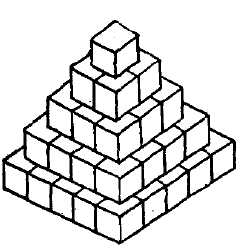
\includegraphics[scale=.7]{1.png}
\end{figure}

\begin{solution}
    显然,这一垛共有:$(1+4+9+16+25)$桶.
即:$1^2+2^2+3^2+4^2+5^2=55$桶.

这就是说,前五个自然数的平方
和等于55.

一般地,如果由前n个自然数的
平方组成的数列$1^2,2^2,3^2,\ldots,n^2$.
如何求出它们的和呢?能不能导出一
个通用的公式呢?

以下我们将先对这个数列的前$n$项和的特点进行
分析,然后应用待定系数法导出它的求和公式.

设$1^2+2^2+\cdots+n^2=S(n)$,在$S(n)$中,$n$代表项数.显然有:
\[\begin{split}
   S(0)&=0\\ S(1)&=1\\ S(2)&=1^2+2^2=5\\ S(3)&=1^2+2^2+3^2=14\\
   \cdots \cdots&\cdots\cdots\\ 
   S(n)&=1^2+2^2+\cdots+n^2\\ 
   S(n+1)&=1^2+2^2+\cdots+n^2+(n+1)^2 
\end{split}\]

而且还可以看出:无论项数$n$取几,总有
\[S(n+1)-S(n)=(n+1)^2=n^2+2n+1\]
可见,$S(n)$很可能是一个关于项数$n$的多项式,
它只要满足两个性质:
\begin{enumerate}
    \item $S(0)=0$
    \item $S(n+1)-S(n)=n^2+2n+1$ ($n$的二次式)
\end{enumerate}
\end{solution}

这就启示我们,如果能求出一个多项式$S(x)$, 能
满足以上两条性质,即$S(0)=0$, $S(x+1)-S(x)$是
一个二次式.那么,所求数列的前$n$项和,就是当$x
=n$时,多项式$S(x)$的值$S(n)$.

但是,满足以上两条性质的多项式$S(x)$应该是
几次多项式呢?

我们不妨设$S(x)$是$m$次多项式,即
\[S(x)=ax^m+bx^{m-1}+\cdots+cx+d\quad (a\ne 0)\]
则:$S(x+1)=a(x+1)x^m+b(x+1)x^{m-1}+\cdots+c(x+1)x+d$
由乘法公式,不难知道:
\[\begin{split}
    S(x+1)&= a(x^m+mx^{m-1}+\cdots +1)+b[x^{m-1}+(m-1)x^{m-2}+\cdots+1]\\
    +\cdots + c(x+1)+d\\
    &=ax^m+(b+am)x^{m-1}+\cdots +(c+\cdots)x+(a+b+\cdots +c+d)\\
\end{split}\]
$\therefore\quad S(x+1)-S(x)=(b+am-b)x^{m-1}+\cdots =amx^{m-1}+\cdots$

由于$am\ne 0$, 显然$S(x+1)-S(x)$是$m-1$次多
项式,因此,我们可以得出:

\begin{blk}{}
    当$S(x)$是一个$m$次多项式时,$S(x+1)-S(x)$必定是一个$m-1$次多项式.
\end{blk}

也就是说,多项式$S(x+1)-S(x)$的次数比多项
式$S(x)$的次数低一次.

这样,由于在我们以上所求问题中,$S(x+1)-S(x)$是二次多项式,所以,
\textbf{$S(x)$必定是一个三次多项式}.

基于以上分析,以下我们就可以用待定系数法导
出前$n$个自然数平方的求和公式.


\begin{example}
    试求$1^2+2^2+\cdots+n^2$.
\end{example}


\begin{solution}
    设$1^2+2^2+\cdots+n^2=S(n)$

由分析知$S(n)$是一个关于项数$n$的三次式,
且 $S(0)=0$, $S(1)=1$, $S(2)=5$, $S(3)=14$.
其中,0是$S(n)$的一个根.

$\therefore\quad $由余式定理的推论,得:
\[S(n)=n(an^2+bn+c)\]
这里$a$、$b$、$c$都是待
定系数.

将$S(1)=1$, $S(2)=5$, $S(3)=14$分别代入上
式,即可得出
\[\begin{cases}
    1=a+6+c\\
5=2(4a+26+c)\\
14=3(9a+36+c)
\end{cases}\Rightarrow\quad \begin{cases}
    a+b+c=1\\
4a+2b+c=\frac{5}{2}\\
9a+3b+c=\frac{14}{3}
\end{cases}\]
解这个方程组,得$a=\frac{1}{3},\quad b=\frac{1}{2},\quad c=\frac{1}{6}$
因此:
\[\begin{split}
    S(n)&=n\left(\frac{1}{3}n^2+\frac{1}{2}n+\frac{1}{6}\right)\\
&=\frac{n}{6}(2n^2+3n+1)\\
&=\frac{1}{6}n(n+1)(2n+1)
\end{split}\]
\end{solution}


\begin{ex}
    试用待定系数法求$1^3+2^3+\cdots+n^3$.
\end{ex}



\section*{习题7.2}
\addcontentsline{toc}{subsection}{习题7.2}
\begin{enumerate}
    \item 已知$x^4+4x^3+6px^2+4qx+r$能被$x^3+3x^2+9x+3$整
    除,试求$p$、$q$、$r$的值.
    \item 已知$f(x)=ax^2+bx+c$是一个完全平方式,试用待定
    系数法证明:$b^2-4ac=0$.
    \item 试用待定系数法把$f(x)=3x^3-10x^2+13$表示成$(x-2)$
    的各次方幂和.
    \item 用待定系数法,把$x^4-2x^2-2$表示成$x^2-x+1$的各
    次方幂和.
    \item 已知$x^3-x^2-8x+12=0$有两个根相等,试解这个方
    程.
    \item 已知方程$x^3-4x^2+x+k=0$有一个根是$-1$, 试求
    它的另外两个根.
    \item  如果方程$x^3+px^2+qx+r=0$有两个根互为相反数,
    试求$p,q,r$应具有什么关系?
    \item  化下列各分式为部分分式
    \begin{multicols}{2}
  \begin{enumerate}
\item  $\frac{3 x-4}{x^{2}-3 x+2}$
\item  $\frac{x^{2}+x-3}{(x-1)(x-2)(x-3)}$
\item $\frac{x^{2}-2}{x^{3}-3 x^{2}+2 x}$
\item  $\frac{x^{3}-6 x^{2}+4 x+8}{(x-3)^{4}}$
\item  $\frac{2 x^{2}+1}{x^{3}-1}$
\item  $\frac{21 x-14}{(x-3)^{2}(2 x+1)}$
\item  $\frac{8 x}{(x+1)\left(x^{2}-1\right)}$
\item  $\frac{x^{2}+x+1}{\left(x^{2}+1\right)\left(x^{2}+2\right)}$
\end{enumerate}      
    \end{multicols}

\item 求下列各算术平方根:
\begin{multicols}{2}
   \begin{enumerate}
    \item  $\sqrt{5+2 \sqrt{6}}$
    \item  $\sqrt{15-2 \sqrt{56}}$
    \item  $\sqrt{11+4 \sqrt{7}}$
    \item  $\sqrt{26-8 \sqrt{10}}$  
\end{enumerate}     
\end{multicols}

\item 求下列数列的前 $n$ 项和:
    $1^{4}, 2^{4}, 3^{4}, \ldots , n^{4}, \ldots$

\end{enumerate}






\section*{本章内容要点}

本章的主要内容是两种常见数列的求和及待定系数法与它的应用.

一、等差数列

\begin{enumerate}
    \item 按顺序排好的一列数中,如果从第二个数
起,每一个数与它前一个数的差都相等,那么,这一列数叫做等差数列.

设等差数列的首项为$a_1$, 公差为$d$, 项数为$n$, 末项为$a_n$及前$n$项和为$S_n$, 则有以下关系式:
\[\begin{split}
    a_n&=a_1+(n-1)d\\
    S_n&=\frac{n}{2}[2a_1+(n-1)d]=\frac{n}{2}(a_1+a_n)
\end{split}\]

如果已知$a_1,a_n,n,d,S_n$中的任意三个,就可以利用这两个公式,求出另两个.

\item 在两个已知数$a,b$之间,插入$n$个数构成等
差数列的问题,实际上就是已知首项$a$, 末项$b$及项数$n+2$, 要求出公差,进而可以求出插入的各项,还可以求出所有项的和.
\end{enumerate}

\vskip 2ex 
二、等比数列

按顺序排好的一列数中,如果从第二个数起,每一个数与它前一个数的比都相等,那么,这一列数叫
做等比数列.

设等比数列的首项为$a_1$, 公比为$q$, 项数为$n$, 末项为$a_n$, 前$n$项的和为$S_n$, 则有以下关系式:
\[\begin{split}
    a_n&=a_1q^{n-1}\\
    S_n&=\frac{a_1(1-q^n)}{1-q}
\end{split}\]

公比$q$的取值,决定了等比数列各项的大小变化趋向:如果首项$a_1>0$(或$<0$),那么,
\begin{itemize}
    \item 当$q>1$时,等比数列逐项增大(或减小);
    \item 当$0<q<1$时,等比数列逐项减小(或增大);
    \item 当$q<0$时,等比数列各项将正、负相间,逐项在正、负值之间摆动.
\end{itemize}

\vskip 2ex 
三、待定系数法是一个重要的数学方法,其根据就是多项式恒等的性质.其方法的要点就是:引进未定系数,列出恒等式并进而得出含有未定系数的方程组,求出未定系数.

待定系数法应用广泛,具体作法中又有一定的技巧,除可以求商式、余式、分解因式、寻求方程的根与系数间的关系外,还应从以下应用中进一步去掌握:
\begin{itemize}
    \item 求多项式与解方程;
    \item    用一个较低次的多项式的各次幂,表示另一个多项式;
    \item     将分式化成部分分式;
    \item 求形如$a\pm 2\sqrt{b}$的数的算术平方根;
    \item 求数列$1^b,\; 2^b,\; 3^b, \ldots,n^b,\ldots$ 前$n$项和($b$是大于1的一个自然数).
\end{itemize}


\section*{复习题七}
\addcontentsline{toc}{section}{复习题七}

\begin{enumerate}
    \item 求下列数列的前 10 项和及第$n$项.
\begin{enumerate}
    \item $0,\;-2,\;-4,\;-6, \ldots$;
    \item $\frac{1}{2},\;-\frac{1}{4},\; \frac{1}{8},\;-\frac{1}{16}, \ldots$;
    \item $-0.1,\;0.1,\;0.3,\;0.5 \ldots$;
    \item $9,\;3,\;1,\; \frac{1}{3},\; \frac{1}{9} \ldots$.
\end{enumerate}

\item 试求出下列数列的第 $n$ 项, 并导出它的前 $n$ 项求和公式:
\begin{enumerate}
    \item $1 \frac{1}{2},\; 2 \frac{1}{4}, \;3 \frac{1}{8} ,\; 4 \frac{1}{16}, \ldots$;
    \item $ 1.3,1.03,1.003,1.0003, \ldots$;
    \item $\frac{1}{1 \times 2},\; \frac{1}{2 \times 3},\; \frac{1}{3 \times 4},\; \frac{1}{4 \times 5},\ldots$.
\end{enumerate}

\item 如果有三个数成等差数列, 又成等比数列, 那么, 你能
    说明这三个数一定相等吗?
    \item 首项为100,公差为$-10$的等差数列中,前多少项的和最大?求出这个和.
\item  如果 $a, b, c$ 分别是一等比数列的第 $p, q, r$ 项, 试说
    明:
    $$a^{q-r} \cdot b^{r-p} \cdot c^{p-q}=1$$
    
    提示:设这一数列的公比为 $t$, 并将$a$视为首项, 则 $b, c$分别是第$q-p+1$、$r-p+1$项.

\item 求和:$S_n=\frac{1}{2}+\frac{2}{2^2}+\frac{3}{2^3}+\frac{4}{2^4}+\cdots+\frac{n}{2^n}$

提示:可以先求$S_n-\frac{1}{2}S_n$


\item 已知$f(-1)=0,\; -5f(0)=-\frac{10}{3}f(-2)=f(-3)=-20$,试求:$f\left(-\frac{1}{2}\right)$及$f\left(-\frac{5}{2}\right)$的值.

\item $\ell$和$m$是何值时,方程$\poly{1,4,-2,\ell ,m}=0$能有两组相等的根?
\item 方程$x^3+px^2+qx+r=0$要有两个根是互为相反数,试问:$p,q,r$必须符合什么条件?

\item 求和:
\[\frac{a}{x(x+a)}+\frac{a}{(x+a)(x+2a)}+\cdots +\frac{a}{[x+(n-1)a](x+na)}\]

提示:$\frac{a}{[x+(n-1)a](x+na)}=\frac{1}{x+(n-1)a}-\frac{1}{x+na}$

\item 将分式 $\frac{\poly{6,5,0,-7}}{\poly{3,-2,-1}}$ 化成部分分式.

\item 证明:如果$a,b,c$成等比数列,那么方程
\[(a^2+b^2)x^2-2b(a+c)x+b^2+c^2=0\]
有两个相等的实数根,且这个实数根正好等于公比.

提示:$a,b,c$之间有关系$b^2=ac$

\end{enumerate}
   \chapter{单变量函数}
前面中我们已经说明了如何由量的度量而产生实数
系.在这一章中我们要进一步说明如何用变数符号去表达变
量,用变数之间的函数关系去表达变量之间的关联.变数是
变量的抽象,函数是变量相互关系的抽象.在这一章里我们
还要运用极限来分析和确立连续函数的概念.

\section{函数的概念}
\subsection{变数和变域}
在研究自然现象时,人们会遇到许多不同的物理量,如
时间、长度、体积、速度、质量、力等等.按照给定条件,
能取许多不同数值的量叫做\textbf{变量};而只取一个数值的量叫做
\textbf{常量},用来表达变量的符号叫做\textbf{变数}.习惯上常用$x,y,
z$等字母表示变数,从纯数学的观点来说,一个变数就是一
个“能取许多不同数值”的符号,它所能取的所有数值构成
一个集合,叫做它的\textbf{变域}.如果变数$x$的变域已经给出,我
们就认为变数$x$是已知的.一般说来,任何数集可以当作变
数的变域.常会遇到取所有自然数的变数$n$, 譬如数列中的
项数.可是在现实生活中,我们通常研究的是连续变化的变
数,如动点所经过的路程及所花的时间等物理量,就是这种
变数的原形,数的区间就是这一类变数的变域,最常用的区
间是以两个实数$a$与$b$ $(a<b)$——它的两个端点——为界
限的有限区间,两个端点本身可以包含在区间内,也可以不
包含在内.因此我们可以把区间分为:
\begin{itemize}
    \item 开区间$(a,b)$就是$\{x|a<x<b\}$;
    \item  闭区间$[a,b]$就是$\{x|a\le x\le b\}$;
    \item  半开区间$(a,b]$就是$\{x|a<x\le b\}$;
    $[a,b)$就是$\{x|a\le x<b\}$.
\end{itemize}
在上述各种情形,数$b-a$为区间的长度.

常量可以看作变量的特殊情形,它的变域是由一个数组
成的集合$\{x|x=a\}$.

数轴上的线段是数的区间的几何表示,图示开区间如图
8.1或8.2.

在点$a,b$处的圆圈或圆括号表示从区间去掉这两个
数.在两个圆圈之间的粗线段表示在$a,b$之间的一切数$x$.
图示闭区间如图8.3.
图示半开区间如图8.4、8.5,每一种情形都只包含出现
有方括号的数,以及在$a,b$之间的一切实数.
\begin{figure}[htp]\centering
    \begin{minipage}[t]{0.48\textwidth}
    \centering
\begin{tikzpicture}[>=latex, scale=.7]
       \draw[->] (0.5,0)--(7.5,0);
       \draw[ultra thick] (2.5,0)node[below=5pt]{$a$}--(5.5,0)node[below=5pt]{$b$};
       \draw (2.5,0)[fill=white] circle (2pt);
        \draw (5.5,0)[fill=white] circle (2pt);
    \end{tikzpicture}
    \caption{}
    \end{minipage}
    \begin{minipage}[t]{0.48\textwidth}
    \centering
    \begin{tikzpicture}[>=latex, scale=.7]
        \draw[->] (0.5,0)--(7.5,0);
        \draw[ultra thick] (2.5,0)node[below=5pt]{$a$}--(5.5,0)node[below=5pt]{$b$};
        \node at (2.5,0){$($}; \node at (5.5,0){$)$};
    \end{tikzpicture}
    \caption{}
    \end{minipage}
    \end{figure}

\begin{figure}[htp]\centering
    \begin{minipage}[t]{0.48\textwidth}
    \centering
\begin{tikzpicture}[>=latex, scale=.7]
    \draw[->] (0.5,0)--(7.5,0);
    \draw[ultra thick] (2.5,0)node[below=5pt]{$a$}--(5.5,0)node[below=5pt]{$b$};
    \node at (2.5,0){$[$}; \node at (5.5,0){$]$};
    \end{tikzpicture}
    \caption{}
    \end{minipage}
    \begin{minipage}[t]{0.48\textwidth}
    \centering
    \begin{tikzpicture}[>=latex, scale=.7]
        \draw[->] (0.5,0)--(7.5,0);
        \draw[ultra thick] (2.5,0)node[below=5pt]{$a$}--(5.5,0)node[below=5pt]{$b$};
        \node at (2.5,0){$($}; \node at (5.5,0){$]$};
    \end{tikzpicture}
    \caption{}
    \end{minipage}
    \end{figure}

\begin{figure}[htp]\centering
    \begin{minipage}[t]{0.48\textwidth}
    \centering
\begin{tikzpicture}[>=latex, scale=.7]
    \draw[->] (0.5,0)--(7.5,0);
    \draw[ultra thick] (2.5,0)node[below=5pt]{$a$}--(5.5,0)node[below=5pt]{$b$};
    \node at (2.5,0){$[$}; \node at (5.5,0){$)$};
    \end{tikzpicture}
    \caption{}
    \end{minipage}
    \begin{minipage}[t]{0.48\textwidth}
    \centering
    \begin{tikzpicture}[>=latex, scale=.7]
        \draw[->] (0.5,0)--(7.5,0);
        \draw[ultra thick] (2.5,0)node[below=5pt]{$a$}--(5.5,0)node[below=5pt]{$b$};
        \node at (2.5,0){$($}; \node at (5.5,0){$)$};
        \draw (4,0)[fill=white] circle (2pt)node[above]{$c$};
    \end{tikzpicture}
    \caption{}
    \end{minipage}
    \end{figure}

有时也要考虑无穷区间,用符号$-\infty,+\infty$作为一端或
两端,它们的记号和上面所引进的相类似,例如$(-\infty,+\infty)$
是全体实数集合$\{x|x\in\mathbb{R}\}$, 区间$(a,+\infty)$表示集
合$\{x|x>a\}$, 区间$(-\infty,b]$表示集合$\{x|x\le b\}$. 无穷区间
在几何上可用两端无限伸延的直线或一端无限伸延的射线来
表示.

以后我们要常用到一点的邻域的概念.\textbf{$c$点的邻域}是包
含$c$点的任何开区间$(a,b)$, 而$c$点的去心邻域指去掉$c$
点的任何$c$点的邻域.它的图象如图8.6.

$c$点的去心邻域可写成$(a,c)\cup (c,b)$. 我们常把
$c$点的邻域写成对称的形式:$(c-r,c+r)$, 对任何
$r>0$, 并且称它为\textbf{$c$点的对称邻域}.

\begin{example}
    试写出含于区间$(1,5)$中$\pi$的对称邻域.
$\left(\pi-\frac{1}{2},\pi+\frac{1}{2}\right)$是含于$(1,5)$的$\pi$对称邻域.此外
$(\pi-1,\pi+1)$, $\left(\pi-\frac{3}{2},\pi+\frac{3}{2}\right)$, $(\pi-0.01,\pi+0.01)$
等都是含于$(1,5)$中的对称邻域.
\end{example}

\subsection{函数的定义}
我们已经在第三册研究过许多函数,例如多项式函数、
三角函数,由于函数这个概念的重要性,并且它将是我们
的主要研究对象,因此需要回忆一般的函数的定义,下面我
们从数集之间的多对一(包括一对一)的关系重新给出函数
定义.

\begin{blk}{定义}
     设有数集$A,B$, 如果有一对应关系或法则$f$存
在,对于$A$的任何一个数$x$, 有数集$B$中唯一的一个数$y$与之
对应,我们就称给出了一个从数集$A$到数集$B$内的函数$f$, 用
\[f:A\mapsto B\]
表示,并写成$y=f(x),\; (x\in A)$, 此时称$f(x)$为函数$f$在$x$的
函数值,并称$A$为函数$f$的\textbf{定义域}.又当$x$取遍$A$中的数时,
函数值$f(x)$全体也构成一个数集,称为函数$f$的\textbf{值域},记作
\[f(A)=\{f(x)|x\in A\}\]
要注意的是在构造一个函数$f:A\mapsto B$的时候,$f(A)$不一定等
于$B$, 而是$B$的一个真子集,即$f(A)\subset B$.
\end{blk}



\begin{example}
设$\mathbb{R}$是实数集,函数$f:\mathbb{R}\mapsto\mathbb{R}$定义为
\[f(x)=\frac{2x}{x^2+1},\quad x\in(-\infty,+\infty)\]
求它的值域.
\end{example}

\begin{solution}
    方程$f(x)=\frac{2x}{x^2+1}$等价于
    \begin{equation}
        yx^2-2x+y=0
    \end{equation}
根据函数的值域定义,任给$y\in f(\mathbb{R})$, 方程(8.1)必有实数
解,而方程(8.1)有实数解的充要条件是
\[\Delta=1-y^2\ge 0\]
即:$-1\le y\le 1$,所以
\[f(\mathbb{R})=\{f(x)|-1\le f(x)\le 1\}\subset \mathbb{R}\]
\end{solution}

在函数的定义中包含三个要素,即\textbf{定义域},\textbf{多对一的对
应法则}和\textbf{函数值所在的数集}.应养成一个习惯,当给定一个
函数时,必须指明它的定义域.在实际问题中,函数的定义
域是根据实际意义来确定的,例如温度计刻有华氏温标度数
$F$和摄氏温标度数$c$,因为不存在低于绝对零度的温度,因
此,这两个度数之间的函数$\varphi$是
\[F=\varphi(c)=\frac{9}{5}c+32,\quad c\in (-273,+\infty)\]

以后,当我们只在数学上,一般地研究一个具体解析式
子规定的函数关系时,如果定义域$A$没有被指明,那么函数
的定义域是使解析式子具有数值意义的所有$x$的数值组成的
自然定义域,函数$y$的值域通常是不指出的,因为由对应的
规律本身就可以确定函数的值域.


\begin{example}
    求下列函数定义域:
\begin{multicols}{2}
\begin{enumerate}
    \item $f(x)=\frac{\sqrt{1-x}}{x}$
    \item $g(x)=\sqrt{x^2-1}$
\end{enumerate}
\end{multicols}
\end{example}

\begin{solution}
    \begin{enumerate}
        \item \[\text{函数$f$有意义}\Leftrightarrow \begin{cases}
    1-x \ge 0\\
    x\ne 0
\end{cases}\Rightarrow\quad x\le 1, \quad x\ne 0\]
$\therefore\quad $函数$f$的定义域为$(-\infty,0)\cup(0,1]$.

\item \[\text{函数$g$有意义}\Leftrightarrow x^2-1\ge 0 \Rightarrow\quad x\le 1, \text{ 或 } x\ge 1\]
$\therefore\quad $函数$g$的定义域为$(-\infty,-1]\cup[1,+\infty)$.
    \end{enumerate}
\end{solution}

\subsection{相等的函数}
怎样的两个函数是相等的函数?在数学中,有些函数可
以用不同的方式来定义,例如,函数$f:\mathbb{R}\mapsto \mathbb{R}^+\cup\{0\}$是由
$f(x)=|x|$规定的,而函数$g:\mathbb{R}\mapsto \mathbb{R}^+\cup\{0\}$是由$g(x)=\sqrt{x^2}$规定的,这里表示$f(x)$与$g(x)$的式子全不同,但是对
于它们的相同的定义域中的任一$x$值,经过不同规则的计算,
它们的结果是相同的,即$f(x)=g(x)$, 所以对于这个例子
来说,尽管函数$f(x),g(x)$的表达式不同,我们说$f(x)$和
$g(x)$表示相同的函数.此外,解析式子相同,但定义域不同
的函数是不相同的函数.例如:
\[\begin{split}
    f_1(x)&=\frac{1}{x},\qquad x\in (-\infty,0)\cup(0,+\infty)\\
    f_2(x)&=\frac{1}{x},\qquad x\in (0,+\infty)\\
    f_3(x)&=\frac{1}{x},\qquad x\in (0,1)
\end{split}\]
是不相同的函数,因为对于$x=-2$, $f_1$有意义而$f_2,f_3$都无
意义;对于$x=2$, $f_1$和$f_2$都有意义而$f_3$无意义.

下面给出相等(同)的两个函数的条件.

\begin{blk}{定义}
    两个函数$f:A\mapsto B$, $g:C\mapsto D$称为相等的当且仅
    当$A=C$, $B=D$, 且对于每个$a\in  A$(或$C$),有$f(a)=g(a)$.
\end{blk}

读者可能会不同意上面$B=D$这个条件,提出下面这个
例子来反驳:

“由$f(n)=g(n)=n$给出的两个函数$f:\mathbb{N}\mapsto\mathbb{N}$, $g: \mathbb{N}\mapsto \mathbb{Q}$是相等的函数”我们须指出两个函数不同的地方,就
函数值所在数集上看,$g$可以除以2, 因此,对于$g$我们可
以构造一个新函数,
$\frac{1}{2}g:\mathbb{N}\mapsto \mathbb{Q}$, 这里
\[\left(\frac{1}{2}g\right)(n)=\frac{1}{2}n\]
但是对于$f$, 不能做这种构造.

\subsection{函数的几个类型——满射、单射和双射}
现在,我们来讨论函数的三个重要类型,先给出定义,
然后再举例说明.

\begin{blk}{定义 }
   如果在函数$f:A\mapsto B$的$B$中的每一个数$b$在函数$f$
的作用下都是$A$中一个数或某些数的对应数,也就是说:对
于任意$b\in B$, 存在一个$a\in A$, 使得$b=f(a)$, 这样我们就说
$f$是由$A$到$B$的\textbf{满射}.
\end{blk}

显然,如果$f:A\mapsto B$是满射,那么$f(A)=B$.

第二类函数和满射同样地重要,叫做\textbf{单射},定义如下:

\begin{blk}{定义}
    如果对于$A$中的任何两个不同的数$a_1$和$a_2$, 就在
$B$中有两个不同的函数值$f(a_1)$和$f(a_2)$, 即任何$a_1,a_2\in A$,
$a_1\ne a2\Rightarrow f(a_1)\ne f(a_2)$, 那么我们就说$f:A\mapsto B$是\textbf{单射}(或
一对一).
\end{blk}

 
它的逆否命题“如果在$B$中有$f(a_1)=f(a_2)$就在$A$中有
$a_1=a_2$, 那么函数$f:A\mapsto B$叫做\textbf{单射}(或一对一).”和上面
的定义等价,也常用来说明函数是一对一的.

还有一类很重要的函数叫做\textbf{双射}.

\begin{blk}{定义}
    函数$f:A\mapsto B$, 如果是满射又是单射,就叫做
    \textbf{双射}.
\end{blk}

\begin{example}
    函数$f:\mathbb{R}\mapsto [-1,1]$, 这里$f(x)=\sin x, x\in\mathbb{R}$
是满射,但不是单射,因为对于
$\sin x=\frac{1}{2}\in [-1,1]$,
就有无穷多个$x=\frac{\pi}{6}+2k\pi$或$\frac{5\pi}{6}+2k\pi\;(k\in\mathbb{Z})$的值和它
对应.
\end{example}

\begin{example}
    函数$f:\mathbb{N}\mapsto\mathbb{N}$, 这里$f(n)=2n$是单射,但不是满射.
\end{example}

\begin{example}
    设$2\mathbb{N}$代表偶数集,函数$f:\mathbb{N}\mapsto 2 \mathbb{N}$, 这里$f(n)=2n$就是一双射.
\end{example}

\section{函数的运算与复合函数}

\subsection{函数的四则运算}

设$f(x),g(x)$是两个$x$的函数,它们的定义域分别为$D_f$
和$D_g$, 我们可以用通常对于“数”
的四则运算得到它们的
和函数$(f+g)(x)$, 差函数$(f-g)(x)$, 积函数$(f\cdot g)(x)$与
商函数$\frac{f}{g}(x),\; g(x)\ne 0$.它们的定义域为$D_f\cap D_g$.

由$f(x),g(x)$的四则运算所得出来的新函数的定义
如下:
\begin{itemize}
    \item $(f+g)(x)=f(x)+g(x)$ (即$(f+g)$在$x$点的值是$f$,
$g$的值的和);
\item $(f-g)(x)=f(x)-g(x)$ (即$(f-g)$在$x$点的值是$f,g$
的值的差);
\item $(f\cdot g)(x)=f(x)\cdot g(x)$ (即$(f\cdot g)$在$x$点的值是$f,g$的
值的积);
\item $(f/g)(x)=f(x)/g(x)$ (即$f/g$在$x$点的值是$f,g$的值
的商,但只有在$g(x)\ne 0$时才有意义).
\end{itemize}

$f+g$, $f-g$和$f\cdot g$的定义域是$f$的定义域和$g$的定义
域的交集.而$f/g$的定义域要从$f$和$g$的定义域的交集中去
掉使$g(x)=0$的值.

\begin{example}
    已知$f(x)=\sqrt{x}$, $g(x)=\sqrt{1-x}$, 求$f+g$,
$f-g$, $f\cdot g$, $\frac{f}{g}$, $\frac{g}{f}$.
\end{example}

\begin{solution}
    $f$和$g$的自然定义域是$D_f=\{x|x\ge 0\}$, $D_g=\{x|x\le 1\}$,$D_f$和$D_g$的交集是$D_f\cap D_g=[0,1]$.
\begin{itemize}
    \item 和:$(f+g)(x)=\sqrt{x}+\sqrt{1-x}$
    \item 差:$(f-g)(x)=\sqrt{x}-\sqrt{1-x}$
    \item  积:$(f\cdot g)(x)=\sqrt{x(1-x)}$
    \item 商:$\frac{f}{g}(x)=\sqrt{\frac{x}{1-x}},\qquad \frac{g}{f}(x)=\sqrt{\frac{1-x}{x}}$
\end{itemize}

$f+g$, $f-g$, $f\cdot g$的定义域是$[0,1]$.因为当$x=1$时,
$g(x)=0$, 所以$\frac{f}{g}$的定义域是$[0,1)$, 同样得到$\frac{g}{f}$的定义域$(0,1]$.
\end{solution}

\begin{example}
设$f(x)=\sin x$, $g(x)=\cos x$,$D_f=(-\infty,+\infty)$,$D_g=(-\infty,+\infty)$,则:
\[\begin{split}
    (f+g)(x)=\sin x+\cos x&=\sqrt{2}\left(\frac{1}{\sqrt{2}}\sin x+\frac{1}{\sqrt{2}}\cos x\right)\\
    &=\sqrt{2}\left(\sin x\cos\frac{\pi}{4}+\cos x\sin\frac{\pi}{4} \right)\\
    &=\sqrt{2}\sin\left(x+\frac{\pi}{4}\right)\\
    (f-g)(x)=\sin x-\cos x&=\sqrt{2}\sin\left(x-\frac{\pi}{4}\right)\\
    (f\cdot g)(x)=\sin x\cdot \cos x&=\frac{1}{2}\sin 2x\\
    \left(\frac{f}{g}\right)(x)=\frac{\sin x}{\cos x}&=\tan x\\
\end{split}\]    

这里$f+g$, $f-g$, $f\cdot g$的定义域是$(-\infty,+\infty)$, $\frac{f}{g}$的定义域是$$\left\{x\big|x\in\mathbb{R},\; x\ne \frac{\pi}{2}+k\pi,\; k\in \mathbb{Z}\right\}$$
\end{example}

\subsection{复合函数}
上面我们是用四则运算来组合已知函数为一个新函数
的,但是构成新的函数的方法,还有一个更重要的运算叫做
组成函数的函数或复合函数法.

我们先从一个简单的例子
说起,火箭从地面上的$L$点垂
直向上发射,火箭$R$在$t$秒后
离开发射点的距离是$h(t)$, 这个函数是已知的.在离发射座
1公里远的地方有一个观测站$O$,我们要求把火箭与观测站
的距离$d$确定为时间$t$的函数(图8.7).
\begin{figure}[htp]
    \centering
\begin{tikzpicture}[thick]
\draw (0,0)node[below]{$L$}--node[below]{1}(4,0)node[below]{$O$}--node[above]{$d$}(0,2.5)node[above]{$R$}--node[left]{$h$}(0,0);
\end{tikzpicture}
    \caption{}
\end{figure}

我们已经知道火箭的垂直高度$h$是$t$的函数$h(t)$, 又火
箭到观测站的距离$d$又是火箭的高度$h$的函数
\[d=\sqrt{1+h^2}\]
因此在时刻$t$, $R$到$O$的距离是
\[d(t)=\sqrt{1+h^2(t)}\]

上面函数$d(t)$是由$h=h(t)$和$d=f(h)=\sqrt{1+h^2}$两个函
数构成的,把其中一个函数$h(t)$代入另一个函数$f(h)$的运算
叫做复合运算,得到的函数$d(t)=f\big(h(t)\big)$叫做$t$的复合
函数.

一般说来,若$z=f(y)$, $y=g(x)$, 且$g(x)$的值域含于
$f(y)$的定义域中,那么对于$g(x)$定义域内的每一个$x$值经过
中间变数$y$, 相应地得到唯一确定的一个值$z$, 变数$z$经过
中间变数$y$而成变数$x$的函数,记为$z=f\big(g(x)\big)$, 这个函
数称为前两个函数的\textbf{复合函数}.应该指出,函数$y=g(x)$的
值域不能超出函数$f(y)$的定义域,这是极重要的.


\begin{example}
    设$z=\sqrt{1+y}$, 它的定义域$D_y=[-1,+\infty)$,
再设$y=x^2-5$, 它的定义域$D_x=(-\infty,+\infty)$, 值域$R=
[-5,+\infty)$. 

作为复合函数$z=\sqrt{1+(x^2-5)}=\sqrt{x^2-4}$,
其定义域只能是$(-\infty,-2]$和$[2,+\infty)$, 这时,$y=x^2-
5$的值域是$[-1,+\infty)$, 它没有超过$D_y=[-1,+\infty)$
的范围,这就是说复合函数$z=f\big(g(x)\big)$的定义域只能由$y=
g(x)$的定义域中那些使$g(x)$属于$z=f(y)$的定义域的$x$
组成.
\end{example}

\begin{example}
已知$f(g)=\frac{1}{g+1}$,$g=g(x)=x^2$.

求$f\big(g(x)\big)$和$g\big(f(x)\big)$.    
\end{example}

\begin{solution}
\[\begin{split}
    f\big(g(x)\big)&=\frac{1}{x^2+1}\\
    g\big(f(x)\big)&=\left(\frac{1}{x+1}\right)^2=\frac{1}{x^2+2x+1}
\end{split}\]
显然,$f\big(g(x)\big)\ne g\big(f(x)\big)$, 这表明函数的复合运算是不满足交换律的.
\end{solution}

\begin{example}
已知$f\left(\sin\frac{x}{2}\right)=\cos x+1$,
求$f\left(\cos\frac{x}{2}\right)$.
\end{example}    

\begin{solution}
    复合函数
$f\left(\sin\frac{x}{2}\right)=\cos x+1=2-2\sin^2\frac{x}{2}$
    是把函
    数$y=\sin\frac{x}{2}$
    代入$f(y)=2-2y^2$中复合而成.现在令
    $y=\cos\frac{x}{2}$代入$f(y)$,得到
\[f\left(\cos\frac{x}{2}\right)=2-2\cos^2\frac{x}{2}=2-(1+\cos x)=1-\cos x\]
\end{solution}    

在函数的运算中,我们介绍了函数的加、减、乘、除和
函数的复合五种运算,从定义来看,我们可以用上述五种运
算,由某一简单而基本的函数去造出多种多样的新函数来,
譬如从常数函数$y=c$和恒等函数$y=x$, 用加、减、乘运算就可
以得出多项式函数.其实我们常常要用到的,并不是把所给的
函数组合成更复杂的函数;而是要把所给的函数分解成更简
单的函数的组合,把要解的问题归于比较简单的问题去解决.


\begin{example}
    将函数$y=x\sin\frac{1}{x}$
分解成比较简单的函数的组
合(引进新的中间变数符号).
\end{example}

\begin{solution}
    $y=x\sin\frac{1}{x}$
    可分解为$f(x)=x$与$g(x)=\sin\frac{1}{x}$
    之积,又$g(x)=\sin\frac{1}{x}$
    可以看作是$g(h)=\sin h$和$h=h(x)=\frac{1}{x}$
    的复合函数,于是原来的函数可以看作下面简单函数的
    组合
    \[F(x)=f(x)\cdot g\big(h(x)\big)\]
    这里$f(x)=x$, $g(h)=\sin h$, $h=h(x)=\frac{1}{x}$.    
\end{solution}

\begin{example}
求函数$\sqrt{x-\sqrt{x+1}-2}$的定义域.
\end{example}

\begin{solution}
设$F(x)=\sqrt{x-\sqrt{x+1}-2}=\sqrt{(x+1)-\sqrt{x+1}-3}$,则$F(x)$可以看作$f(y)=\sqrt{y^2-y-3}$与$y=g(x)=\sqrt{x+1}$
的复合函数,即$F(x)=f\big(g(x)\big)$且知:

$f(y)$的定义域
$D_f=\left(-\infty,\frac{1-\sqrt{13}}{2}\right]\bigcup\left[\frac{1+\sqrt{13}}{2},+\infty\right)$

$g(x)$的定义域$D_g=[-1,+\infty)$, 它的值域$R_x=[0,+\infty)$

\[\begin{split}
&\text{复合函数$F(x)=f\big(g(x)\big)$有意义}\Longleftrightarrow
\begin{cases}
    g(x)\text{有意义}\\
    g(x)\in\left[\frac{1+\sqrt{13}}{2},+\infty\right)
\end{cases}\\
&\Longleftrightarrow
\begin{cases}
    x+1\ge 0\\
    \sqrt{x+1}\ge \frac{1+\sqrt{13}}{2}
\end{cases}\Longleftrightarrow
\begin{cases}
    x\ge -1\\
    x+1\ge \left(\frac{1+\sqrt{13}}{2}\right)^2=\frac{7+\sqrt{13}}{2}
\end{cases}\\
&\Longleftrightarrow x\ge \frac{5+\sqrt{13}}{2}
\end{split}\]
$\therefore\quad $函数$\sqrt{x-\sqrt{x+1}-2}$的定义域是
$\left[\frac{5+\sqrt{13}}{2},+\infty\right)$.

如果直接求$F(x)=\sqrt{x-\sqrt{x+1}-2}$的定义域,那
么只须:
\[\begin{split}
   x-\sqrt{x+1}-2\ge 0& \Longleftrightarrow x-2\ge \sqrt{x+1} \Longleftrightarrow \begin{cases}
    x-2\ge 0\\ x+1\ge 0\\ (x-2)^2\ge (x+1)
\end{cases}\\
& \Longleftrightarrow \begin{cases}
    x\ge 2\\x\ge -1\\ x\ge \frac{5+\sqrt{13}}{2}
\end{cases} \Longleftrightarrow x\ge \frac{5+\sqrt{13}}{2}
\end{split}\]
$\therefore\quad $函数$\sqrt{x-\sqrt{x+1}-2}$的定义域是
$\left[\frac{5+\sqrt{13}}{2},+\infty\right)$.
\end{solution}

\section*{习题8.1}
\addcontentsline{toc}{subsection}{习题8.1}

试确定下面1---5里每一对函数$f$和$g$的自然定义域,并
求$f+g$, $f-g$, $f\cdot g$, $f/g$和$g/f$的相应的定义域.

\begin{enumerate}
    \item $f(x)=x,\qquad g(x)=\sqrt{x-1}$
    \item $f(x)=\frac{1}{x-2},\qquad g(x)=\frac{1}{\sqrt{x-1}}$
        \item $f(x)=\sqrt{x},\qquad g(x)=\sqrt[4]{x+1}$
    \item $f(x)=\sin x,\qquad g(x)=\cos x$
    \item $f(x)=\tan x,\qquad g(x)=\tan x$
    \item 证明函数$f(x)=\frac{1}{1+x}$在它的定义域上是单射的.又
    $x$为何值时,下列各式才有意义?
    \begin{multicols}{2}
\begin{enumerate}
    \item $f\big(f(x)\big)$
    \item $f\left(\frac{1}{x}\right)$
    \item $f(cx)$
    \item 对于哪些数$c$,有一数$x$
    能使$f(cx)=f(x)$
\end{enumerate}        
    \end{multicols}

\item 下列函数能否构成复合函数$y=f\big(\varphi(x)\big)$, 如果能够
构成,则指出复合函数的定义域和值域:
\begin{enumerate}
    \item $y=f(u)=2u+1,\qquad u=\varphi(x)=x^2$
    \item $y=f(u)=\sqrt{u},\qquad u=\varphi(x)=1-x^2$
    \item $y=f(u)=u^2+u^3, \qquad u=\varphi(x)=\begin{cases}
        1,& \text{当$x$为有理数}\\
        2,&\text{当$x$为无理数}\\
    \end{cases}$
    \item $y=f(u)=2$, 定义域为$U_1$,\qquad  $u=\varphi(x)$, 定义域为
    $X$, 值域为$U_2$.
\end{enumerate}

\item 设$f(x)=ax^2+bx+c$, 证明
$f(x+3)-3f(x+2)+3f(x+1)-f(x)=0$.
\item \begin{enumerate}
\item 设$y=f(x)=a+bx+\frac{c}{x}$, 求$f\left(\frac{2}{x}\right)$.
\item 设$y=f(x)=\sqrt{1+x+x^2}$, 求$f(x^2)$, $f(-x^2)$.
\end{enumerate}

\item 若$\varphi(x)=x^3+1$, 求$\varphi(x^2)$, $\big(\varphi(x)\big)^2$, $\varphi\big(\varphi(x)\big)$.
\item 求下列函数定义域:
\begin{multicols}{2}
 \begin{enumerate}
    \item $y=\sqrt{x}+\sqrt{-x}$
    \item $y=\sqrt[4]{\frac{(x-2)(x-3)}{x^2}}$
\end{enumerate}   
\end{multicols}

\item $a,b,c,d$取什么值,才能使函数$$f(x)=\frac{ax+b}{cx+d}$$对所有$x$满足$f\big(f(x)\big)=x$?
\end{enumerate}

\section{函数的图象}

从平面上一条曲线(对这条曲线应该要求:与纵轴平行
的直线与它的交点不能多于一个)可以引出一个函数,反过
来,给了一个函数$y=f(x)$, 那么通常采用直角坐标系,就
可以用图形来表示$y$是$x$的函数.

定义在某一变域$D$上的函数的图象就是让$x$取遍$D$中所
有值,所有点$(x,f(x))$的集合便形成平面上的一个\textbf{图形},
这个图形称为函数$y=f(x)$的\textbf{图象},而这个方程$y=f(x)$称
为\textbf{图象的方程}.

利用函数图象的几何直观可以更清楚地看出函数的一些
性质,下面我们把函数的解析性质和它的图象上相应的几何
性质对照着列出来:
\begin{center}
\begin{tabular}{cp{.45\textwidth}p{.45\textwidth}}
    \hline
    &  解析性质  &几何性质\\
    \hline
    1  &$f$是$x$的增函数,即对于任意的$a\in D$, $b\in D$, 当$a<b$时,恒有$f(a)<
f(b)$  &$f$的图象随着$x$向右移动而上升\\
2&$f$是$x$的减函数,即对于任意的$a\in D$, $b\in D$, 当$a<b$时,恒有$f(a)>f(b)$ &$f$的图象随着向右移动而下降\\
3&$f$是偶函数,即对于任意的$x\in D$, 恒有$f(-x)=f(x)$ &函数$f$的图象关于$y$轴对称\\
4& $f$是奇函数,即对于任意的$x\in D$, 恒有$f(-x)=-f(x)$ & 函数$f$的图象关于原点对称\\
5 & $f$是周期函数,即对于任意的$x\in\mathbb{R}$, 恒有$f(x+p)=f(x)$, 这里$p$是一个正的常数& 函数$f$在区间
$[0,p]$或$\left[-\frac{p}{2},\frac{p}{2}\right]$上的
图象可以沿$x$轴左、右连续推移,重复出现\\
\hline
\end{tabular}
\end{center}

下面我们给出几个常见的函数的图象.

\subsubsection{常值函数}
常值函数$f(x)=c$的图象是一条平行$x$轴的直线,它
至$x$轴的距离为$|c|$, 如图8.8.

\subsubsection{取整函数}
函数$f(x)=[x]$代表不超过$x$的最大整数,即:
若$n\le x<n+1,\; n\in\mathbb{Z}$, 则$f(x)=[x]=n$. 它的图象
如图8.9.

\begin{figure}[htp]\centering
    \begin{minipage}[t]{0.48\textwidth}
    \centering
\begin{tikzpicture}[>=latex, scale=1]
\draw[->] (-2.5,0)--(2.5,0)node[right]{$x$};
\draw[->] (0,-1)--(0,2.5)node[right]{$y$};
\draw[very thick] (-2,1.5)--(2,1.5)node[above]{$f(x)=c$};
\draw[<->] (-1,0)--node[right]{$c$}(-1,1.5);
\node at (-.25,-.25){$O$};
    \end{tikzpicture}
    \caption{}
    \end{minipage}
    \begin{minipage}[t]{0.48\textwidth}
    \centering
    \begin{tikzpicture}[>=latex, scale=1]
        \draw[->] (-2.5,0)--(3.5,0)node[right]{$x$};
        \draw[->] (0,-2.5)--(0,2.5)node[right]{$y$};
    \foreach \x in {-2,-1,1,2,3}
    {
        \draw (\x,0)node[below]{$\x$}--(\x,.1);
    }     
\foreach \x in {1,2}
{
    \draw (0,\x)node[left]{$\x$}--(.1,\x);
}
\foreach \x in {-1,-2}
{
    \draw (0,\x)--(.1,\x)node[right]{$\x$};
}

\foreach \x in {-2,-1,...,2}
{
    \draw [very thick](\x,\x)--(\x+1,\x);
    \draw (\x+1,\x)[fill=white] circle(1.5pt);
}
\node at (-.25,-.25){$O$};
    \end{tikzpicture}
    \caption{}
    \end{minipage}
    \end{figure}

\subsubsection{一次函数}

我们已经在第三册中知道,一次函数$f(x)=kx+b\; (k\ne 0)$的图象是不平行于$x$轴和$y$轴的直线.$k$称为直线的斜
率,$b$称为直线的$y$截距.若知一次函数图象上的两个点,
我们用直线方程的两点式:
\[y-y_1=\frac{y_2-y_1}{x_2-x_1}(x-x_1)\]
就可以写出一次函数的关系式.

下面给出的函数的图象是有间断点的直线:

函数$f(x)=\frac{3}{4}\cdot \frac{x^2-1}{x-1}$, 
$x\in (-\infty,1)\cup(1,+\infty)$的
图象是一条有间断点$\left(1,1\frac{1}{2}\right)$的直线,除去点$\left(1,1\frac{1}{2}\right)$外,
它与直线$y=\frac{3}{4}(x+1)$一致.(见图8.10)

\begin{figure}[htp]
    \centering
    \begin{tikzpicture}[>=latex, scale=1]
        \draw[->] (-2.5,0)--(3,0)node[right]{$x$};
        \draw[->] (0,-1)--(0,2.5)node[right]{$y$};
\foreach \x in {-1,1}
{
    \draw (\x,0)node[below]{$\x$}--(\x,.1);
}
\draw[domain=-2:2, samples=10, very thick]plot(\x, {0.75*(\x+1)});

\draw[dashed] (0,1.5)node[left]{$1\frac{1}{2}$}--(1,1.5)--(1,0);
\draw (1,1.5) [fill=white] circle(1.5pt)node[right]{$\left(1,1\tfrac{1}{2}\right)$};
\node at (2,2)[above]{$y=\frac{3}{4}(x+1)$};
        \node at (.25,-.25){$O$};
            \end{tikzpicture}    
    \caption{}
\end{figure}

\subsubsection{阶梯函数}
设点列$\{x_i\},\; i=0,1,\ldots,n$是闭区间$[a,b]$中的递增
点列,使得$x_0=a$, $x_n=b$, 即
$a=x_0<x_1<x_2<\cdots<x_{n-1}<x_n=b$,且当$x_{i-1}<x<x_i$时,
$f(x)=k_i,\; i=1,2,\ldots,n$.而$x$在分点,$x_i,\; i=0,1,\ldots,n$的
值$f(x_i)$可以任意给定,这样一个在$[a,b]$上有定义的,而
在每个子区间$(x_{i-1},x_i),\; i=1,2,\ldots,n$都是常数的函数叫
做阶梯函数.

例如,定义在$[0,6]$上的阶梯函数$f$:
\[\begin{cases}
   f(0)=2.5,\\
f(x)=2 ,&0<x\le 1,\\
f(x)=0,&1<x\le 2,\\
f(x)=-1,&2<x\le 4,\\
f(x)=2 ,&4<x\le 6. \\
\end{cases}\]
的图象如图4.11所示.

\begin{figure}[htp]\centering
    \begin{minipage}[t]{0.48\textwidth}
    \centering
\begin{tikzpicture}[>=latex, scale=.73]
    \draw[->] (-.5,0)--(7,0)node[right]{$x$};
    \draw[->] (0,-1.5)--(0,3.5)node[right]{$y$};
\foreach \x in {1,2,...,6}
{
\draw (\x,0)node[below]{$\x$}--(\x,.1);
}
\node at (-.25,-.25){$O$};
\foreach \x in {-1,1,2,2.5}
{
\draw (0,\x)node[left]{$\x$}--(.1,\x);
}

\draw[very thick] (0,2)--(1,2);
\draw[very thick] (1,0)--(2,0);
\draw[very thick] (2,-1)--(4,-1);
\draw[very thick] (4,2)--(6,2);
\foreach \x in {{0,2},{1,0},{2,-1},{4,2}}
{
\draw (\x)[fill=white] circle(2.5pt);
}
\draw (0,2.5)[fill=black] circle(2.5pt);
    \end{tikzpicture}
    \caption{}
    \end{minipage}
    \begin{minipage}[t]{0.48\textwidth}
    \centering
    \begin{tikzpicture}[>=latex, scale=.73]
        \draw[->] (-.5,0)--(7,0)node[right]{$x$};
        \draw[->] (0,-5)--(0,2)node[right]{$y$};
\foreach \x in {1,2,...,6}
{
    \draw (\x,0)node[below]{$\x$}--(\x,.1);
}
\node at (-.25,-.25){$O$};
\foreach \x in {1,-1,-2,...,-4}
{
    \draw (0,\x)node[left]{$\x$}--(.1,\x);
}

\draw[very thick] (1,0)node[above]{$A$}--(2,.5)node[above]{$B$}--(3,-1)node[below]{$C$}--(4,0)node[above]{$D$}--(6,-4)node[below]{$E$};

    \end{tikzpicture}
    \caption{}
    \end{minipage}
    \end{figure}

\subsubsection{折线函数}
我们定义$g$:
\[g(x)=\begin{cases}
    \frac{1}{2}(x-1), & x\in[1,2]\\
    -\frac{3}{2}(x-2)+\frac{1}{2}(2-1),& x\in [2,3]\\
    (x-3)-\frac{3}{2}(3-2)+\frac{1}{2}(2-1),& x\in [3,4]\\
  -2(x-4)+(4-3)-\frac{3}{2}(3-2)+\frac{1}{2}(2-1),& x\in [4,6]\\
\end{cases}\]
它的图象是一条折线$ABCDE$, 如图4.12.


\subsubsection{幂函数}
函数$f(x)=x^n$,其中$n$为任意自然数,称为正整指数幂
函数.

为了了解正整指数幂函数的一般性质,我们在同一个坐
标系内,绘出几个这样的函数,如图4.13.

显然,当$n$为奇数时,因为$f(-x)=(-x)^n=-x^n=-f(x)$,
所以函数是奇函数.又所有正整指数幂函数,当$x=0$时,
$f(0)=0$.故每个奇次幂函数的图象通过原点,位于第一和
第三象限内且关于原点对称.所有这样的函数都是增函数.

当$n$为偶数时,因为$f(-x)=(-x)^n=x^n=f(x)$,所以
函数是偶函数,每个图象通过原点,位于第一和第二象限内
且关于$y$轴对称.

由于当$x=1$时,$f(1)=1^n=1$, 每个正整指数幂函数的
图象都通过点$(1,1)$.

\begin{figure}[htp]
    \centering
    \begin{tikzpicture}[>=latex, scale=3]
        \draw[->] (-1.3,0)--(1.3,0)node[right]{$x$};
        \draw[->] (0,-1.3)--(0,1.3)node[right]{$y$};
\foreach \x in {-1,1}
{
    \draw (\x,0)node[below]{$\x$}--(\x,.02);
}
\node at (.1,-.1){$O$};
\draw[dashed](-1,-1)--(-1,1)--(1,1)--(1,0);

\draw (-1.2,-1.2)--(1.2,1.2);
\draw [domain=-1.15:1.15, samples=100, thick]plot(\x, {\x*\x});
\draw [domain=-1.1:1.1, samples=100, very thick]plot(\x, {\x*\x*\x});
\draw [domain=-1.05:1.05, samples=100, ultra thick]plot(\x, {\x*\x*\x*\x});
\node at (0,1)[right]{1};
\node at (1,1)[right]{$(1,1)$};
\node at (-.75,-.75)[right]{$y=x$};
\node at (-.8,-.512)[left]{$y=x^3$};
\node at (-.75,.5625)[right]{$y=x^2$};
\node at (-.8,.41)[left]{$y=x^4$};
            \end{tikzpicture}    
    \caption{}
\end{figure}

现在让指数$n$逐次增大,看看图象的变化,从图8.14,
8.15可以清楚地看出每个图象的平坦部分和陡峭部分,曲线
最终以图8.14和8.15中的粗黑线为极限位置.

函数$f(x)=x^{-n}$($x\ne 0$, $n$为自然数)称为负整指数幂函数.
在同一坐标系内,绘出$y=x^{-1}$, $y=x^{-2}$, $y=x^{-3}$, $y=x^{-4}$
的图象如图8.16所示.当$x=0$时,这些函数都无意义,函数
的图象在此点断开,它的二支以$y$轴为渐近线.

当指数为负奇数时,这些函数是奇函数.图象的二支分
别位于第一和第三象限内,随$x$向右移动下降,且关于原点
对称.因此,函数在$(-\infty,0)$或$(0,+\infty)$内是减函数.

当指数是负偶数时,这些函数是偶函数,每个函数的图
象在原点处断开,分为二支,位于第一和第二象限内,都以
$y$轴为渐近线,且关于$y$轴对称.从图象明 显地看出,当
$x<0$时,函数是增函数,当$x>0$时,函数是减函数.

下面我们来说明一些函数的图象如何由另一些函数的已
知图象经过某些几何变换得到.

若对于任意的$x\in D$, 函数$f$和$g$满足$g(x)=f(x-c)$,
这里$c$是常数,则若$c>0\; (c<0)$,$y=g(x)$的图象可以由
$y=f(x)$的图象,平行$x$轴右移(或左移)$|c|$个单位得到.

若函数$f$和$g$满足等式$g(x)=f(kx)$, 这里$k$是常数,则若
$k>1\; (0<k<1)$, $y=g(x)$的图象可以由$y=f(x)$的图象经
过把它上面的所有点的横坐标垂直于$y$轴压缩(或拉长)倍
而纵坐标不变的几何变换得到.

若函数$f$和$g$满足等式,$g(x)=kf(x)$, 这里$k$是常数,
则若$k>1\; (0<k<1)$, $y=g(x)$的图象可以由$y=f(x)$的图
象经过把它上面的所有点的纵坐标垂直$x$轴拉长(或压缩)
$k$倍而使横坐标不变的几何变换得到.

下面我们用例子说明图象的几何变换.
\begin{figure}[htp]\centering
    \begin{minipage}[t]{0.48\textwidth}
    \centering
\begin{tikzpicture}[>=latex, scale=2.2]
    \draw[->] (-1.3,0)--(1.3,0)node[right]{$x$};
    \draw[->] (0,-.5)--(0,1.6)node[right]{$y$};
\foreach \x in {-1,1}
{
\draw (\x,0)node[below]{$\x$}--(\x,.02);
}
\node at (.1,-.1){$O$};
\draw[ultra thick](-1,1.5)--(-1,0)--(1,0)--(1,1.5);
\draw [domain=-1.25:1.25, samples=100, thick]plot(\x, {\x*\x});
\draw [domain=-1.15:1.15, samples=100, dashed]plot(\x, {\x*\x*\x*\x});
\node at (-.75,.5625)[right]{$y=x^2$};
\node at (-1.2,1.7)[right]{$y=x^4$};      
    \end{tikzpicture}
    \caption{}
    \end{minipage}
    \begin{minipage}[t]{0.48\textwidth}
    \centering
    \begin{tikzpicture}[>=latex, scale=2]
        \draw[->] (-1.3,0)--(1.3,0)node[right]{$x$};
        \draw[->] (0,-1.3)--(0,1.3)node[right]{$y$};
\foreach \x in {-1,1}
{
    \draw (\x,0)node[below]{$\x$}--(\x,.02);
}
\node at (.1,-.1){$O$};
\draw[ultra thick](-1,-1.2)--(-1,0)--(1,0)--(1,1.2);
\draw (-1.2,-1.2)--(1.2,1.2);
\draw [domain=-1.1:1.1, samples=100, thick]plot(\x, {\x*\x*\x});
\node at (0,1)[right]{1};
\node at (.75,.75)[left]{$y=x$};
\node at (.8,.512)[right]{$y=x^3$};
    \end{tikzpicture}
    \caption{}
    \end{minipage}
    \end{figure}

\begin{figure}[htp]
    \centering
\begin{tikzpicture}[>=latex, scale=1.2]
    \draw[->] (-4,0)--(4,0)node[right]{$x$};
    \draw[->] (0,-5)--(0,5)node[right]{$y$};
\draw [domain=-4:-.22, samples=100]plot(\x, {1/\x});
\draw [domain=-3.5:-.45, samples=100, thick]plot(\x, {1/(\x*\x)});
\draw [domain=-3:-.6, samples=100, very thick]plot(\x, {1/(\x*\x*\x)});
\draw [domain=-3:-.68, samples=100, ultra thick]plot(\x, {1/(\x*\x*\x*\x)});  
\node at (.2,-.2){$O$};
\draw [domain=.22:4, samples=100]plot(\x, {1/\x});
\draw [domain=.45:3.5, samples=100, thick]plot(\x, {1/(\x*\x)});
\draw [domain=.6:3, samples=100, very thick]plot(\x, {1/(\x*\x*\x)});
\draw [domain=.68:3, samples=100, ultra thick]plot(\x, {1/(\x*\x*\x*\x)});  

\draw[dashed](1,0)--(1,1)node[right]{$(1,1)$}--(-1,1)node[left]{$(-1,1)$}--(-1,-1)node[left]{$(-1,-1)$}--(0,-1);

\draw (1,-1)--(1.5,-1)node[right]{$y=x^{-1}$};
\draw[thick] (1,-1.5)--(1.5,-1.5)node[right]{$y=x^{-2}$};
\draw[very thick]  (1,-2)--(1.5,-2)node[right]{$y=x^{-3}$};
\draw[ultra thick]  (1,-2.5)--(1.5,-2.5)node[right]{$y=x^{-4}$};
\draw (.75,-.6) rectangle (3,-2.9);


\end{tikzpicture}
    \caption{}
\end{figure}



\begin{example}
    说明$y=f(x)=\sin x$和$y=g(x)=\cos x$的图象的
关系.
\end{example}


\begin{solution}
 这两个函数的定义域都是$(-\infty,+\infty)$,根据$f(x)=
\sin x$和$g(x)=\cos x$是周期等于$2\pi$的函数,因此我们可以先在
长度等于$2\pi$的区间上来讨论这两个函数.

设$f(x)=\sin x$的定义域$D_y=[0,2\pi]$, 因为余弦函数
$g(x)=\cos x$可以看作正弦函数$\sin x$ 与$x'=x+\frac{\pi}{2}$
的复合函数,即$g(x)=\cos x=\sin\left(x+\frac{\pi}{2}\right)$,
所以复合函数$\sin\left(x+\frac{\pi}{2} \right)$
有意义,必须且只须$0\le x+\frac{\pi}{2}\le 2\pi$,
由此得到$-\frac{\pi}{2}\le x\le \frac{3\pi}{2}$.

这就是说$y=g(x)=\cos x$ 的定义域是
$D_g=\left[-\frac{\pi}{2},\frac{3\pi}{2}\right]$.
因为区间$D_g$是把区间$D_f$左移了$\frac{\pi}{2}$
个单位的结果,并且对于$D_g=\left[-\frac{\pi}{2},\frac{3\pi}{2}\right]$中
的每一个$x$都可以在$D_f=[0,2\pi ]$中找
到相应的$x+\frac{\pi}{2}$
使得
$\cos x=\sin\left(x+\frac{\pi}{2}\right)$,
所以$y=\sin x$在
区间$D_f=[0,2\pi]$ 上的一段图象左移
$\frac{\pi}{2}$个单位就得到$y=\cos x$在区间$D_g=
\left[-\frac{\pi}{2},\frac{3\pi}{2}\right]$上
的一段,因此,将$y=\sin x$的整个图象左移$\frac{\pi}{2}$
个单位就得到整个$y=\cos x$的图象了,如图
8.17所示.
\begin{figure}[htp]
    \centering
\begin{tikzpicture}[>=latex, scale=.8]
    \draw[->] (-5.5,0)--(9,0)node[right]{$x$};
    \draw[->] (0,-2)--(0,2)node[right]{$y$};
    \foreach \x/\xtext in {-3/-\tfrac{3\pi}{2},-1/-\tfrac{\pi}{2},1/\tfrac{\pi}{2},3/\tfrac{3\pi}{2},5/\tfrac{5\pi}{2}}
    {
        \draw(\x*pi/2, 0)node[below]{$\xtext$}--(\x*pi/2,.2);
    }
    \foreach \x/\xtext in {-1/-\pi, 1/\pi, 2/2\pi}
    {
        \draw(\x*pi, 0)--(\x*pi,.2)node[above]{$\xtext$};
    }
    \draw [domain=-pi:2.5*pi, samples=100, very thick]plot(\x, {cos(\x r)});
    \draw [domain=-1.5*pi:2.5*pi, samples=100,  thick]plot(\x, {sin(\x r)});
    \node at (.4,-.4){$O$};
 \node at (-pi,-1)[below]{$y=\cos x$};
 \node at (2.5*pi,1)[right]{$y=\sin x$};
\end{tikzpicture}    
    \caption{}
\end{figure}

$\because\quad \sin(-x)=-\sin x,\qquad \therefore\quad y=\sin x$的图象关于原点对称.

$\because\quad \cos(-x)=\cos x,\qquad \therefore\quad y=\cos x$的图象关于$y$轴对称.

\end{solution}

\begin{example}
    说明函数$y=f(x)=\sqrt{1-x^2}$, $D_f=[-1,1]$和
    $y=g(x)=\sqrt{1-4x^2}$的图象的关系.
\end{example}

\begin{solution}
    我们已经知道$f$的定义域是$D_f=[-1,1]$且$g(x)$可
以看作$f(x')$与$x'=2x$的复合函数,即
\[g(x)=f(2x)=\sqrt{1-(2x)^2}\]

复合函数$f(2x)$有意义必须且只须$-1\le 2x\le 1$, 即:
\[-\frac{1}{2}\le x\le \frac{1}{2}\]
因此,$g(x)$的定义域是$D_g=\left[-\frac{1}{2},\frac{1}{2}\right]$.
因为对于$D_g=\left[-\frac{1}{2},\frac{1}{2}\right]$中
的每一个$x$, 在$D_f$中一定有一个相应的$2x$使
得$g(x)=f(2x)$成立,这就说明了将$y=f(x)$的图象上所有
点的横坐标垂直$y$轴压缩一半而使点的纵坐标不变便得
$g(x)=\sqrt{1-4x^2}$的图象,如图4.18所示.

\begin{figure}[htp]
    \centering
\begin{tikzpicture}[>=latex, scale=2.5]
    \draw[->] (-1.5,0)--(1.5,0)node[right]{$x$};
    \draw[->] (0,-.5)--(0,1.5)node[right]{$y$};
\draw [very thick](-1,0) arc (180:0:1);
\draw[domain=-.5:.5, samples=1000, thick] plot(\x, {sqrt(1-4*\x*\x)});
\foreach \x/\xtext in {-1/-1,-.5/-\frac{1}{2},.5/\frac{1}{2},1/1}
{
    \draw (\x,0)node[below]{$\xtext$}--(\x,.1);
}
\node at (.1,-.1){$O$};

\draw[thick] (1,1)--(1.25,1)node[right]{$y=g(x)=\sqrt{1-4x^2}$};
\draw[very thick] (1,1.25)--(1.25,1.25)node[right]{$y=f(x)=\sqrt{1-x^2}$};
\draw (.9,.8) rectangle (2.7,1.4);
\end{tikzpicture}
    \caption{}
\end{figure}
\end{solution}

\begin{ex}
\begin{enumerate}
    \item 试由函数增减性的定义,说明下面函数的增减性:
    \begin{multicols}{2}
\begin{enumerate}
    \item $y=x^3$
    \item $y=x^{-2}$
    \item $f(x)=\sqrt{x}$
    \item $g(x)=\sqrt[3]{x}$
    \item $h(x)=\frac{1}{\sqrt{x}}$
\end{enumerate}        
    \end{multicols}

    \item 作下列函数的图象:
    \begin{multicols}{2}
        \begin{enumerate}   
\item $y=\sqrt{x}$
\item $y=x-[x]$
\item $y=\sqrt{x-[x]}$
\item $y=[x]+\sqrt{x-[x]}  $
        \end{enumerate}        
    \end{multicols}
    \item 若一折线函数的图象$ABCDE$的顶点坐标是
\[A\left(-1,-1\frac{1}{2}\right),\quad B(1,1),\quad C(3,-1),\quad D(6,2.5),\quad E(7,2.5)\]    
写出这个函数的解析式.

\item 作下列函数的图象:
\begin{multicols}{2}
    \begin{enumerate}  
\item $f(x)=|2x|$
\item $f(x)=\frac{|x|}{x}$
\item $y=|4-x^2|,\quad -3\le x\le 3$
\item $y=|x^2-2x-3|$
\end{enumerate}        
\end{multicols}
\item 已知点$P(\alpha,\beta)$和一水平线$L$即$g(x)=\gamma$的图象.证
明至$P$与$L$等距离的所有点$(x,y)$的集合,是具有$f(x)=
ax^2+bx+c$形式的函数的图象.
\end{enumerate}
\end{ex}

\section{函数的连续性}
在初中一年级讨论平方根时,我们曾用下面的想法初步
地肯定$\sqrt{2}$的“存在性”:边长是1米的正方形面积是1平
方米;边长是2米的正方形面积是4平方米,所以,当一个正
方形的边长逐渐增加时,它的面积逐渐由1平方米增加到4
平方米,中间应该会有那么一个2平方米的正方形.

上面这段话只是一个粗略的想法,用数学语言来表达
如下:

$y=f(x)=x^2$, 这个幂函数的函数值,在$x=1$时,$f(1)=1^2=1$;
$x=2$时,$f(2)=2^2=4$; 当$x$由1变到2时,$x$的值应
该由1“连续地”变到4, 所以$x$应该能取一个值$x_0$使
$f(x_0)=x^2_0=2$.

上面说的“连续地”这个术语究竟是什么意思呢?在这
一节中,我们就是要把“连续性”的涵意加以分析、确立.
并且,把上面这个粗略的想法体现成一个明确有用的定
理——中间值定理.

\subsection{连续函数的概念}
从几何的直观来看,连续与间断的意思是一目了然的,
一条曲线是连续的,指这条曲线没有间断点,在上一节考察
的函数,展示了函数图象有间断点的情形,函数$f$在点$x_0$是
否连续只依赖于它在$x_0$的一个(任意小的)邻域内的变化情
况.直观地看来,如果
\begin{enumerate}
\item $f$在其定义域的点$x_0$的邻域$(x_0-\delta,x_0+\delta)$内
有定义;
\item 当$x$充分接近$x_0$时,函数值$f(x)$同$f(x_0)$相差任
意小,即自变量$x$的微小变化只能引起函数值的微小变化,
从而排除了函数值的跳跃,就函数的图象来看,在这一点
$x_0$的邻近,函数图象是由一条曲线组成的,而没有在这一点
断开成为两个分支,那么称函数$f$在点$x_0$连续.
\end{enumerate}


“充分接近”和“相差任意小”这两句话是不够明确的,而
必须用定量的术语给以严格的表述.现在我们可以用数列极
限的概念把“当$x$充分接近$x_0$时,$f(x)$与$f(x_0)$相差任意小”
这句话定量地描述如下:

如果在函数定义域$I$中,自变量$x$取任何一个收敛于$x_0\in I$
(即$\displaystyle\lim_{i\to\infty}x_i=x_0$)的数列$\{x_i\}$的项$x_i\; (i=1,2,\ldots)$, 那么对应
的函数数列:
\[f(x_1),\; f(x_2),\; \ldots,\;  f(x_i),\ldots\]
总有极限值$f(x_0)$, 即
\[\lim_{i\to\infty} f(x_i)=f(x_0)\]

于是我们得到下述连续性的严格定义:

\begin{blk}{定义}
     定义在区间$I$上的一个函数$f$在点$a\in I$称做连
续,如果
\begin{enumerate}
\item $f(a)$有一个确定值,
\item 对于$I$中每一个收敛于$a$的数列$\{x_i\}$, 对应的函数
数列$\{f(x_i)\}$总以$f(a)$为极限,即有关系式:
$\displaystyle\lim_{i\to \infty}f(x_i)=f(a)=f\left(\displaystyle\lim_{i\to \infty}x_i\right)$
成立.
\end{enumerate}
\end{blk}


这个定义表明对于一个连续函数$f$, 记号lim可以和记号
$f$互换.

我们举几个例子说明如何用这个定义来验证函数$f$在点
$a$处连续或间断.


\begin{example}
    函数$f(x)=\frac{3}{4}\cdot\frac{x^2-1}{x-1}$
在点$x=1$处不连续,因为
$f(1)$没有意义.
\end{example}

\begin{example}
    函数$f(x)=[x]$在整数点$n$处不连续,因为当
$x=n,\; (n\in\mathbb{Z})$时,函数$f(x)=[x]$有确定值$f(n)=[n]=n$.
虽然当$x$取的数列$\{x_i\}$的值,从$x=n$的右边趋于$n$时,
有$\Lim_{i\to\infty}f(x_i)=\Lim_{i\to\infty}[x_i]=n=f(n)$, 但是当$x$取的数列$\{x'_n\}$从$x=n$的左边趋于$n$时,即当$x'_i$满足条件:$n-1\le x'_i <m$, $\Lim_{i\to \infty}x'_i=n$时,那么
\[\Lim_{i\to \infty}f(x'_i)=\Lim_{i\to \infty}[x'_n]=n-1\ne f(n)=n\]
这就是说$f(x)=[x]$的图象是在整数点具有跳跃性间断的
曲线.
\end{example}

现在我们来考虑另一种间断性的曲线.
\begin{example}
    函数$f(x)=\frac{1}{x}$
    在点$x=0$处不连续,因为$f(0)$不
    存在,并且任何数列$\{x_i\}$收敛于0时,例如:
    
    当$x_i>0$, $x_i\to 0$时,即$x_i$从右边趋近于原点时,有
$\Lim_{i\to\infty}\frac{1}{x_i}=+\infty$;

    当$x_i<0$, $x_i\to 0$时,即$x_i$从左边趋近于原点时,有
    $\Lim_{i\to\infty}\frac{1}{x_i}=-\infty$;

    当$\{x_i\}$是任意一个趋于0的数列时,则$\Lim_{i\to\infty}\left|\frac{1}{x_i}\right|=\infty$.

    无论哪种情形,数列$\left\{\frac{1}{x_i}\right\}$
    趋向无穷大.
\end{example}

\begin{rmk}
例8.16和例8.18的分母的零点都是函数的不连续点,
但是例8.16中的分式:$f(x)=\frac{3}{4}\cdot\frac{x^2-1}{x-1}$,
当$x=1$时,代数恒等式
\[\frac{3}{4}\cdot\frac{x^2-1}{x-1}=\frac{3}{4}(x+1)\]
是成立的.因此任何数列$x_i\; (\ne 1)$趋于1时,由于$x_i\ne 1$,
\[\begin{split}
    \Lim_{i\to\infty}f(x_i)&=\Lim_{i\to\infty}\frac{3}{4}\cdot \frac{x^2_i-1}{x_i-1}=\Lim_{i\to\infty}\frac{3}{4}(x_i+1)\\
    &=\frac{3}{4}(1+1)=\frac{3}{2}
\end{split}\]

这就是说,对于任何收敛于1的数列$\{x_i\}$, 对应的函数数
列$\{f(x_i)\}$都以$\frac{3}{2}$为极限. 

如果我们定义一个新函数$F$:
\[F(x)=\begin{cases}
    \frac{3}{4}\cdot\frac{x^2-1}{x-1},& x\ne 1\\
    \frac{3}{2}, & x=1
\end{cases}\]
那么$F(x)$在点$x=1$处就连续了.
\end{rmk}

\begin{blk}{定义}
     如果对于任何收敛于$a$的数列$\{x_i\}$, $\Lim_{i\to\infty}f(x_i)$存在,并且彼此相等,但不等于$f(a)$, 或者$f(a)$没有定义,则
称$f$在$a$处有可去间断点.
\end{blk}

例8.16中的$x=1$就是$f$的可去间断点.

\begin{blk}{定义}
    如果函数$f$在定义域$I$中每一点都连续,就说$f$
是$I$上的一个连续函数,或简称为连续函数.
\end{blk}

\subsection{连续函数的运算}
由连续函数定义知道,函数$f$在$a\in I$连续当且仅当:若
$I$里的每个数列$\{x_i\}$收敛于$a$时,数列$\{f(x_i)\}$也收敛于
$f(a)$.

我们可以把上述条件:
\[\lim_{i\to \infty}x_i=a \quad \Longrightarrow\quad \lim_{i\to \infty}f(x_i)=f(a)\]
简写成:
\[\lim_{x\to a}f(x)=f(a)=f\left(\lim_{x\to a}x\right)\]

由数列极限运算定理直接得出下面定理.

\begin{blk}{定理1}
    设$f$和$g$在$a$处连续,即
    \[\lim_{x\to a}f(x)=f(a),\qquad \lim_{x\to a}g(x)=g(a)\]
    则
\begin{enumerate}
    \item $\Lim_{x\to a}[f(x)\pm g(x)]=f(a)\pm g(a)$,(即$f\pm g$在$a$处连续).
    \item $\Lim_{x\to a}f(x)\cdot g(x)=f(a)\cdot g(a)$,(即$f\cdot g$在$a$处连续).
    \item 若$g(a)\ne 0$,$\Lim_{x\to a}\frac{1}{g(x)}=\frac{1}{g(a)}$,(即$1/g$在$a$处连续).
\end{enumerate}
\end{blk}

\begin{example}
    函数$f(x)=x^k$ ($k$是一个正整数,$x\in\mathbb{R}$) 到处连
续,即$\Lim_{x\to a}x^k=a^k,\; (a\in\mathbb{R})$.
\end{example}

\begin{proof}
对$k$用数学归纳法来证明,设$a$是$f$的定义域$\mathbb{R}$
中任何一点.

当$k=1$时,显然,$\Lim_{x\to a}x=a$, 命题成立.

假设当$k=i\; (i\in\mathbb{N})$时,有
\[\Lim_{x\to a} x^i=a^i\qquad (i\in\mathbb{N})\]
那么,当$k=i+1$时,有
\[\Lim_{x\to a}x^{i+1}=\Lim_{x\to a} x^i\cdot x=\Lim_{x\to a} x^i\cdot \Lim_{x\to a} x=a^i\cdot a=a^{i+1}\]    
于是,对于所有正整数$k$, $f(x)=x$在任何一点$a$连续,也
即$f(x)=x$到处连续.
\end{proof}


由定理1和$f(x)=x^k\; (k\in\mathbb{N})$, 及常数函数$g(x)=c$ ($c$是常数)的到处连续性,我们可以证明下面的命题
成立.

\begin{blk}{命题1}
    任何多项式函数到处连续.
\end{blk}

进一步推得下面命题:

\begin{blk}{命题2}
    若$f$和$g$是两个多项式,$g\ne 0$, 那么有理函
数$r=f/g$,
除去$g$的零点集合,函数$r$是有定义的而且是
连续的.
\end{blk}

\begin{blk}{命题3}
    $f(x)=\sqrt[n]{x}$在区间$(0,+\infty)$上连续,即 
\[\lim_{x\to x_0}\sqrt[n]{x}=\sqrt[n]{x_0}\qquad (x\in[0,+\infty))\]
\end{blk}

\begin{proof}
    设$x_0$是一个任给正数,数列$\{x_i\}$是在$[0,+\infty)$
内任何一个收敛到$x_0$的数列,即$\Lim_{i\to \infty} x_i=x_0$.我们要证明,当
$\Lim_{i\to\infty} x_i=x_0$时,$\Lim_{i\to\infty} (\sqrt[n]{x_i}-\sqrt[n]{x_0})=0$.

在代数恒等式:
\[(A-B)\left(A^{n-1}+A^{n-2}B+\cdots +AB^{n-2}+B^{n-1}\right)=A^n-B^n\]
中,以$A=x_i^{\tfrac{1}{n}}$, $B=x_0^{\tfrac{1}{n}}$代入,即得:
\begin{equation}
\sqrt[n]{x_i}-\sqrt[n]{x_0}=\frac{x_i-x_0}{x_i^{\tfrac{n-1}{n}}+x^{\tfrac{n-2}{n}}_i\cdot x_0^{\tfrac{1}{n}}+\cdots +x^{\tfrac{1}{n}}_i\cdot x_0^{\tfrac{n-2}{n}} + x_0^{\tfrac{n-1}{n}}} 
\end{equation}
由于$\Lim_{i\to\infty}x_i=x_0$, 根据数列极限定义,取
$\varepsilon=\frac{x_0}{2}$,
则存在正整数$N$, 使得当$i>N$时,有
\[x_i>x_0-\frac{x_0}{2}=\frac{x_0}{2}\]
从而,当$i>N$时,有
\begin{equation}
    (x_i)^{\tfrac{1}{n}}=\left(\frac{x_0}{2}\right)^{\tfrac{1}{n}}
\end{equation}
此外,显然有
\begin{equation}
    (x_0)^{\tfrac{1}{n}}=\left(\frac{x_0}{2}\right)^{\tfrac{1}{n}}
\end{equation}

由(8.2)---(8.4)立即得
\[\left|\sqrt[n]{x_i}-\sqrt[n]{x_0}\right|<\frac{|x_i-x_0|}{n\left(\sqrt[n]{\frac{x_0}{2}}\right)^{n-1}}\]
当$i\to\infty$时,$|x_i-x0|\to 0$, 又因为$n\left(\sqrt[n]{\frac{x_0}{2}}\right)^{n-1}$
是一个和$i$
无关的常数,所以
\[\left|\sqrt[n]{x_i}-\sqrt[n]{x_0}\right|\to 0\]
即
\[\lim_{x\to x_0} \sqrt[n]{x}=\sqrt[n]{x_0}\]
这也就证明了$f(x)=\sqrt[n]{x}$ 在区间$[0,\infty)$上到处连续.
\end{proof}

我们在这里介绍了函数连续性的严格定义,对于初学者
只要能够正确理解这一分析定义的涵义就可以了,以后在第
六册微积分中,我们还要对它进行研究.

\subsection{连续函数的中间值定理}
平面上一个一目了然的性质是:一条直线把平面分割成
两半,例如,在$(x,y)$坐标平面上,直线$y=c$就把平
面分成$y<c$和$y>c$这两半,从上半平面走到下半平面的
连续通路,必须和分界线$y=c$相交,下述中间值定理也就
是上述直观现象的代数化:

\subsubsection{中间值定理}

设$y=f(x)$是一个在闭区间$[a,b]$
上到处连续的函数,设$c$是一个介于$f(a)$和$f(b)$之
间的常数,则必存在一个介于$a,b$之间的实数$x_0$, 使得
$f(x_0)=c$.用几何术语来说:$y=f(x)$, $a\le x\le b$的图象
是一条还结$P(a,f(a))$点和$Q(b,f(b))$点的连
续曲线,而$P,Q$分居于直线$y=c$的两侧,则曲线$y=
f(x),\; a\le x\le b$至少和直线$y=c$有一个交点$(x_0,
f(x_0)=c)$,(图8.19).

\begin{figure}[htp]
    \centering
\begin{tikzpicture}[>=latex, yscale=1.3]
    \draw[->] (-1,0)--(6,0)node[right]{$x$};
    \draw[->] (0,-1)--(0,2)node[right]{$y$};
    \draw(-1,1)--(5,1)node[right]{$y=c$};
    \node at (.25,-.25){$O$};
    \draw[ thick] plot[smooth] coordinates{(-.5,-.5)(0,.2) (.5,.5) (1.5,.45) (2.4,1.2)(3.3,.7)(4.6,1.2)};
\node at (-.5,-.5)[below]{$P(a,f(a))$};
\node at (4.6,1.3)[above]{$Q(b,f(b))$};
\draw[dashed] (2.8,0)node[below]{$x_0$}--(2.8,1);
\end{tikzpicture}
    \caption{}
\end{figure}


在给出这个定理的证明之前,我们先讨论一个特例,让
$f(x)=x^3+x-3$, $a=1$, $b=2$. 由于$f(1)=-1$与$f(2)=7$异号,我们将说明在1,
2之间一定存在$f(x)=x^3+x-3$的根$k$, 使$f(k)=0$.

从$y=x^3+x-3$的图象
(图8.20)上看,这个命题是一
目了然的,现在我们要把二分
逼近法与实数完备性,函数连
续性配合一起来说明它的根的
存在和根的求法.

\begin{figure}[htp]
    \centering
\begin{tikzpicture}[>=latex, yscale=.6]
\draw[->] (-2,0)--(3,0)node[right]{$x$};
\draw[->] (0,-9)--(0,8)node[right]{$y$};
\foreach \x in {-8,-7,...,-1,1,2,...,7}
{
    \draw (-.1,\x) node[left]{$\x$} --(0,\x);
}
\node at (.4,-.4){$O$};
\draw[domain=-1.6:2, samples=100, very thick] plot(\x, {\x*\x*\x+\x-3});
\node at (2,5)[right]{$y=x^3+x-3$};
\end{tikzpicture}
    \caption{}
\end{figure}


首先,我们容易验证这个
方程没有整数根$\pm 1$和$\pm 3$, 
因此所求的根一定是一个无理
数,由于闭区间$[a,b]=
[1,2]$具有性质$P:f(a)\cdot f(b)<0$, 即$f(a)$与
$f(b)$异号.当我们把它二
等分时,至少会有一个分段保
有这个性质$P$, 照这样,不断地二等分保有性质$P$的分段,
我们就可以得到保有性质$P$的两串左、右夹逼数列如下:

令$x=\frac{1+2}{2}=\frac{3}{2}$, 
显然$f\left(\frac{3}{2}\right)\ne 0$, 否则$f(x)$就
会有有理数根$\frac{3}{2}$,
无论$f\left(\frac{3}{2}\right)$是正还是负,在$\left[1,\frac{3}{2}\right]$和$\left[\frac{3}{2},2\right]$
这两个分段中一定有一段具有性质$P$, 算出
\[f\left(\frac{3}{2}\right)=\frac{3}{8}>0\]

取$a_1=1$, $b_1=\frac{3}{2}$, 
闭区间$[a_1,b_1]=\left[1,\frac{3}{2}\right]$
保有性质$P$, 照这样进行有限次后,由于$f(x)$没有有理根,
所以$f\left(\frac{a_m+b_m}{2}\right)\ne 0$, 这就使我们每次由$[a_m,b_m]$选取保
有性质$P$的一个分段$[a_{m+1},b_{m+1}]$之后,还可以细分下去,
因此,这个过程是无终止的.
\begin{itemize}
\item 令$x=\frac{a_1+b_1}{2}=\frac{1+\frac{3}{2}}{2}=\frac{5}{4}$,算出$f\left(\frac{5}{4}\right)=\frac{13}{64}>0$,取$[a_2,b_2]=\left[1,\frac{5}{4}\right]$;
\item 
令$x=\frac{a_2+b_2}{2}=\frac{1+1.25}{2}=1.125$, 算出$f\left(1.125\right)=-0.4512<0$,取$[a_3,b_3]=\left[1.125,1.25\right]$;
\item 
令$x=\frac{a_3+b_3}{2}=\frac{1.125+1.25}{2}=1.1875$, 算出$f\left(1.1875\right)=-0.1379<0$,取$[a_3,b_3]=\left[1.1875,1.25\right]$;
\item 
令$x=\frac{1.1875+1.25}{2}=1.2188$, 算出$f\left(1.2188\right)=0.029>0$,取$[a_4,b_4]=\left[1.1875,1.2188\right]$;

\item 
令$x=\frac{1.1875+1.2188}{2}=1.203$, 算出$f\left(1.203\right)=-0.0552<0$,取$[a_5,b_5]=\left[1.203,1.2188\right]$;

\item 
令$x=\frac{1.203+1.2188}{2}=1.211$, 算出$f\left(1.211\right)=-0.0132<0$,取$[a_6,b_6]=\left[1.211,1.2188\right]$;

\item 
令$x=\frac{1.211+1.2188}{2}=1.215$, 算出$f\left(1.215\right)=0.008>0$,取$[a_7,b_7]=\left[1.211,1.215\right]$;

\item 
令$x=\frac{1.211+1.215}{2}=1.213$, 算出$f\left(1.213\right)=-0.0025<0$,取$[a_8,b_8]=\left[1.213,1.215\right]$;

\end{itemize}

这样继续下去,我们得到无穷个闭区间满足下面的
条件:
\begin{enumerate}
    \item $[a,b]=[1,2]\supseteq [a_1,b_1]=\left[1,\frac{3}{2}\right]\supseteq [a_2,b_2]=\left[1,\frac{5}{4}\right]\supseteq [a_3,b_3]=\left[1.1875,1.25\right]
    \supseteq [a_4,b_4]=\left[1.1875,1.2188\right]\supseteq [a_5,b_5]=\left[1.203,1.2188\right]\supseteq [a_6,b_6]=\left[1.211,1.2188\right]\supseteq [a_7,b_7]=\left[1.211,1.215\right]\supseteq [a_8,b_8]=\left[1.213,1.215\right]\supseteq   \cdots 
    \supseteq  
    [a_n,b_n]=\supseteq\cdots $
    \item $[a_n,b_n]=\frac{1}{2}[a_{n-1},b_{n-1}]=\frac{1}{2^2}[a_{n-2},b_{n-2}]=\cdots=\frac{1}{2^n}[a,b]$
    
    因此,闭区间$[a_n,b_n]$的长$=\frac{1}{2^n}\to 0$.
    \item $f(a_n)<0$,\; $f(b_n)>0$恒成立.
\end{enumerate}

换言之,得到满足下面性质的夹逼数列$\{a_n\}$, $\{b_n\}$:
\begin{enumerate}
    \item $a=1\le a_1=1\le a_2=1\le a_3=1.1875\le a_4=1.1875  \le  a_5=1.203  \le  a_6=1.211  \le  a_7=1.211  \le  a_8=1.213  \le\cdots\le a_n\le\cdots\le b_n\le \cdots \le  b_8=1.215  \le  b_7=1.215  \le  b_6=1.2188  \le  b_5=1.2188   \le  b_4= 1.2188  \le  b_3= 1.25 \le  b_2=1.25  \le  b_1=1.5  \le  b=2$
    
    并且$(b_n-a_n)=\frac{1}{2^n}\to 0$.

\item $f(a_n)<0$,\; $f(b_n)>0$恒成立.
\end{enumerate}

由1和实数完备性,就得到唯一实数$k$满足
\[a_n\to k\leftarrow b_n,\qquad \text{即}\quad \lim_{n\to\infty} a_n=\lim_{n\to\infty}  b_n=k\]
再由函数$f(x)=x^3+x-3$的到处连续性,即有
\[\lim_{n\to\infty}  f(a_n)=f(k) \qquad  \lim_{n\to\infty}  f(b_n)=f(k)\]
\begin{itemize}
    \item 由$f(a_n)<0$得知$f(k)\le 0$,
    \item 由$f(b_n)>0$得知$f(k)\ge 0$.
\end{itemize}
所以只有$f(k)=0$才能同时满足上述两种条件.

仿照上面的推理,我们得到了连续函数中间值定理的
证明如下:

为了叙述方便,我们不妨设$f(a)<f(b)$.[当
$f(a)>f(b)$时,我们可以对$-f(x)$和$-c$来作同
样的讨论].由图8.19所示,交点可能有好几个,但是我们
所要证的是至少有一个交点,我们将用二分法去逼近其中一
个交点的坐标$x_0$.

取$a_1=a$, $b_1=b$, 把闭区间$[a,b]$二等分.
\begin{itemize}
    \item 若
$f\left(\frac{a_1+b_1}{2}\right)=c$, 则
就是一个所求的$x_0$, 自
然不必再费任何手脚了;
\item 若
$f\left(\frac{a_1+b_1}{2}\right)<c$,
则取后半段为$[a_2,b_2]$;
\item 若
$f\left(\frac{a_1+b_1}{2}\right)>c$,
则取前半段为$[a_2,b_2]$.
\end{itemize}
照这样逐次地由$[a_m,b_m]$去求出它的半段为$[a_{m+1},b_{m+1}]$.
因为$f(a_m)<c$, $f(b_m)>c$, 取$x_0=\frac{a_m+b_m}{2}$
\begin{itemize}
    \item 若$f\left(\frac{a_m+b_m}{2}\right)<c$
则取后半段为$[a_{m+1},b_{m+1}]$;
\item 若$f\left(\frac{a_m+b_m}{2}\right)>c$
则取前半段为$[a_{m+1},b_{m+1}]$;
\item 若$f\left(\frac{a_m+b_m}{2}\right)=c$
则$\frac{a_{m}+b_{m}}{2}$也就是所求的$x_0$, 
而定理得证.
\end{itemize}

总结上述逐步二等分过程,就只有两种可能:一种可能
是经过有限次二等分后,有这样的分点$\frac{a_m+b_m}{2}$
使$f\left(\frac{a_m+b_m}{2}\right)=c$, 于是定理得证,另一种可能是没有这样的
分点$\frac{a_m+b_m}{2}$
使$f\left(\frac{a_m+b_m}{2}\right)=c$成立,在这种情形下,继
续不断二等分,我们得到无限多个退缩闭区间套$[a_n,b_n]$满
足下列条件:

\begin{enumerate}
    \item 闭区间的端点形成夹逼数列$\{a_n\}$, $\{b_n\}$, 适合
    \[a_1\le a_2\le \cdots\le a_n\le \cdots \le b_n\le \cdots\le b_2\le b_1\]
并且$(b_n-a_n)\to 0$.
    \item $f(a_n)<c$, $f(b_n)>c$恒成立.

\end{enumerate}

    由条件1和数完备性就得到唯一实数$x_0$
    \[\lim_{n\to\infty} a_n=\lim_{n\to\infty} b_n=x_0\quad \text{即}\quad a_n\to x\leftarrow b_n\]
    再由函数$f(x)$在$x_0$连续性即有
\[    \lim_{n\to\infty} f(a_n) = f(x_0),\qquad \lim_{n\to\infty} f(b_n)=f(x_0)\]

由$f(a_n)<c$, 得知它的极限值$f(x_0)\le c$, 同样地,由
    $f(b_n)>c$, 得知它的极限值$f(x_0)\ge c$.

所以,只有$f(x_0)=c$才能同时满足上述两个条件,定理得证.


\begin{blk}{命题1}
    当$a>0$时,$f(x)=x^n-a=0$存在唯一的正实
    数根,叫做$a$的$n$次算术方根,用符号$\sqrt[n]{a}$表示.
\end{blk}

\begin{proof}
    先证存在性.$f(0)=-a<0$, 而
\[f(1+a)=(1+a)^n-a>0\]
所以,由中间值定理$f(x)=x^n-a$在0和$(1+a)$之间至少
有一个根$x_0$, 使得$f(x_0)=x_0^n-a=0$成立.

再证唯一性.因在$x>0$时,$x$愈大则它的$n$次方幂$x^n$
也愈大,所以$f(x)$在$x>0$时是严格递增的,当然不可
能有两个不同的正实数满足$f(x)=0$.
\end{proof}

上面的命题给常用的“$n$次方根函数$y=\sqrt[n]{x},\; x\ge0$”
提供了理论基础.为了进一步把中间值定理应用到一般的多
项式函数上,我们给出下面的命题.

\begin{blk}{命题2 }
对于实系数的多项式
$f(x)=a_0x^n+a_1x^{n-1}+\cdots+a_n,\quad (a_0\ne 0)$, 总可以求出
一个正数$P$, 使得当$x>P$时,$f(x)$的值与$a_0x^n$的值有相同的
符号.
\end{blk}

\begin{proof}
$f(x)=x^n[a_0+\varphi(x)]$, 这里
$\varphi(x)=\frac{a_1}{x}+\frac{a_2}{x^2}+\cdots+\frac{a_n}{x^n},\; (x\ne 0)$是一个$\frac{1}{x}$的
实系数多项式.显然,
\[\lim_{x\to\infty} \varphi(x)=0\]
这也就是说,对于给定的$\varepsilon=|a_0|$, 存在一个正数$P$, 使得
当$x>P$时,从而$0<\frac{1}{x}<\frac{1}{P}$时,有
\[|\varphi(x)|<|a_0|\]
于是$a_0+\varphi(x)$, $(x>P)$与$a_0$同号,因此$f(x)$与$a_0x^n$
同号.
\end{proof}

但是要具体地求出$P$的值,还得用一些技巧.
令$g=\max(|a_1|,|a_2|,\ldots,|a_n|)$, 并且先设$x>P>
1$, 于是$0<\frac{1}{x}<\frac{1}{P}<1$, 从而
\[\begin{split}
    |\varphi(x)|&=\left|\frac{a_1}{x}+\frac{a_2}{x^2}+\cdots+\frac{a_n}{x^n}\right|\\
    &\le g\left(\frac{1}{x}+\frac{1}{x^2}+\cdots+\frac{1}{x^n}\right)< g\cdot \frac{\frac{1}{x}}{1-\frac{1}{x}}
\end{split}\]
要使
\[|\varphi(x)|<g\cdot \frac{\frac{1}{x}}{1-\frac{1}{x}}<|a_0|\]
只须$\frac{1}{x}<\frac{|a_0|}{g+|a_0|}$,即$x>1+\frac{g}{|a_0|}$.

取$P=1+\frac{g}{|a_0|}$,因此,当$x>1+\frac{g}{|a_0|}$时,就可以使$f(x)$与$a_0x^n$有相同符号.

如果令$x=-X\; (X>0)$, 前面的情形说明当$X$是一个
充分大的正数时,$f(-X)$的值的符号就与$(-1)^na_0X^n$
的值有相同符号.因此我们得到下面的推论:

\begin{blk}{推论}
    对于实系数多项式$f(x)=a_0x^n+a_1x^{n-1}+\cdots+a^n\; (a_0\ne 0)$
\begin{itemize}
    \item 当$x$充分大时,$f(x)$与$a_0$同号;
    \item 当$x$取负值而$|x|$充分大时,若$n$是偶数,则$f(x)$与$a_0$同
号;若$n$是奇数,则$f(x)$与$a_0$异号.
\end{itemize}
\end{blk}

由上面的推论直接得到下面的命题:
\begin{blk}{命题2}
    若$n$为奇数,则实系数方程$x^n+a_1x^{n-1}+a_2x^{n-2}+\cdots+a_0=0$
有一个根. 
\end{blk}

\section*{习题8.2}
\addcontentsline{toc}{subsection}{习题8.2}
\begin{enumerate}
    \item 证明下列各函数是到处连续的函数:
\begin{multicols}{2}
\begin{enumerate}
    \item $f(x)=|x|$
    \item $g(x)=\frac{x^2}{1+x^2}$
    \item $h(x)=x|x|-\frac{1}{2}$
    \item $\varphi(x)=\sqrt{x}$
\end{enumerate}
\end{multicols}

\item 设函数$f(x)=\frac{x^2+1}{2x-1}$, 
则$f(0)=-1$, $f(1)=2$
符号相反,讨论方程式$f(x)=0$在$0\le x\le 1$中是否有解?
\item 下列函数各在哪些点不连续:
\begin{multicols}{2}
\begin{enumerate}
    \item $f(x)=\frac{x+2}{x^2-1}$
    \item $f(x)=\frac{x-1}{(x^2+1)(2x+3)}$
    \item $g(x)=\sqrt{\frac{x-2}{x^2-4}}$
    \item $h(x)=\frac{2}{|x|-1}$
    \item $\varphi(x)=\frac{|x|-1}{|x-1|-4}$
    \item $F(x)=\frac{1}{x-[x]}$
\end{enumerate}
\end{multicols}

\item 试证下列多项式有唯一的正实根.
\begin{multicols}{2}
    \begin{enumerate}
        \item $x^3+x^2-1=0$;
        \item $x^3-3x^2+3x-4=0$.
\end{enumerate}
\end{multicols}
\item 证明$8x^3-4x^2-18x+9=0$的一根在0和1之间,一
根在1和2之间,一根在$-2$和$-1$之间.
\item 对于下列各多项式函数$f$, 求一整数$n$使在$n$和
$n+1$之间的某一$x$满足$f(x)=0$:
\begin{multicols}{2}
    \begin{enumerate}
        \item $f(x)=x^3-x+3$;
        \item  $f(x)=x^5+x+1$.
\end{enumerate}
\end{multicols}
\item 设$f(x),g(x)$是两个连续函数而且$f(a)>
g(a)$, $f(b)<g(b)$, 求证在$a,b$之间存在一个适当
$x_0$, 使得$f(x_0)=g(x_0)$.

\item 设$a<b<c$, 证明方程
$\frac{1}{x-a}+\frac{1}{x-b}+\frac{1}{x-c}=2$
有三个实根,且一个根在$a,b$之间,另一个根在$b,c$
之间.
\item 用二分逼近法求$x^3+2x-7=0$的正根,使得 误差小
于0.01.

\end{enumerate}


\section{反函数和它的图象}

在研究一个问题的时候,不只是把两个变量之间的函数
关系表示成$y$是$x$的函数,有时也需要把$x$表示为 $y$的函
数,例如,在自由落体运动中,如果想从已知的时间$t$来确
定路程$s$, 则$s$是$t$的函数
\begin{equation}
    s=\frac{1}{2}gt^2
\end{equation}
如果反过来,
想从已知的路程$s$来确定下落的时间$t$, 则应从(8.5)式将$t$
解出:
\begin{equation}
    t=\sqrt{\frac{2s}{g}}
\end{equation}
这时,$t$是$s$的函数.

从这里看出,这两个函数$s=f(t)=\frac{1}{2}gt^2$和$t=g(s)=
\sqrt{\frac{2s}{g}}$,
其实是同一种关系的两种表示法,我们把这样的两
个函数$f$和
$g$ 叫做互为反函数.

\begin{example}
    若$x\in\mathbb{R}$, $y\in\mathbb{R}$, 那么,函数
\[f:\; y=f(x)=2x+3,\qquad g:\; x=g(y)=\frac{y-3}{2}\]
互为反函数.
\end{example}


\begin{example}
 若$x\in X=\{x|0\le x\le 1\}$, $y\in Y=\{y|0\le y\le 1\}$,而$x,y$之间的关系是$x^2+y^2=1$, 则函数
\[\begin{split}
  f:\; y&=f(x)=\sqrt{1-x^2}\\
g:\; x&=g(y)=\sqrt{1-y^2}   
\end{split}\]
互为反函数,因为在上述关系$x^2+y^2=1$中,$x,y$是对称的,
所以$f$和$g$是同一形式的函数.在一般情况下$f$和$g$是不同
形式的函数.
\end{example}

必须注意,不能认为从每一个函数$y=f(x)$都能解得一
个反函数$x=g(y)$. 例如,如果两个变数$x,y$之间的关系是
$y=x$, 定义域$X=\{x|x\in\mathbb{R}\}$, 值域$Y=\{y|y\ge 0\}$, 那么:
$f:\; y=x,\; x\in (-\infty,+\infty)$是$X\mapsto Y$的函数.但是,如果
不对自变数$x$加以限制,这个函数$f$是不可逆的,也就是由它
不能得到一个新函数$g:\; Y\mapsto X$. 因为,对于每个$y(\ne 0)\in Y$, 
将有$X$中两个数值$x=\sqrt{y}$和$x=-\sqrt{y}$和$y$对应,
如下图所示:

\begin{figure}[htp]
    \centering
    \begin{tikzpicture}[>=latex]
\draw (0,0) ellipse [x radius=1, y radius=1.5];
\draw (4,0) ellipse [x radius=1 ,y radius=1.5];

\draw(0,1)to [bend left=15] node[above]{$f$} (4,.7);
\draw (0,.5)to [bend left=-15]node[above]{$f$} (4,.7);
\draw (0,-1)to [bend left=-15]node[below]{$f$}(4,-.7);
\draw (0,-.5)to [bend left=15]node[below]{$f$} (4,-.7);

\draw[->](1.75,0)--(2.25,0);

\foreach \x/\xtext in {1/2,.5/-2,-.5/a,-1/-a}
{
    \draw (0,\x) [fill=white]circle (1.5pt)node[left]{$\xtext$};
}
\foreach \x/\xtext in {.7/4,-.7/2}
{
    \draw (4,\x) [fill=white]circle (1.5pt)node[right]{$\xtext$};
}
    \end{tikzpicture}
    \caption{}
\end{figure}


下面我们来说明具有怎样性质的函数才有反函数.

假如函数$y=f(x)$具有这样的性质:“若$x_1\ne x_2\; \Rightarrow\; f(x_1)\ne f(x_2)$, 也就是说对于定义域$X$中任意不同的$x_1$, $x_2$, 它们在值域$Y=f(X)$中的对应值$f(x_1)$, $f(x_2)$也不相同”.那么
对于$Y=f(X)$内任何一个$y$, 通过函数$f$, 可以逆对应出一
个且只有一个$x$, 使得$y$和这个$x$对应,这样一个函数叫做由
$X$到$Y=f(X)$的一一对应函数,或双射(满射且单射),简
称这个函数是\textbf{可逆}的.对于一个可逆函数$f:\; x\mapsto f(x)$, 我
们可以交换自变数与因变数的地位,于是对于$Y=f(X)$的
每一个$y$就有$X$内唯一一个逆象$x$, 这就是说我们得到了一
个新函数:
\[ g:\; Y=f(X)\mapsto X,\qquad \text{使得}\; y\mapsto x=g(y)\]
假如$y=f(x)$.

新函数和原来函数的这种关系可以用下图来说明:
\begin{center}
    \begin{tikzpicture}
        \node (A) at (1,0) {$x$};
       \node[rectangle, draw] (B) at (2,0) {$f$};
       \node (C) at (4,0) {$y=f(x)$};
       \node[rectangle, draw] (D) at (6,0) {$g$};
       \node (E) at (7,0) {$x$};    
       \draw (A)--(B)--(C)--(D)--(E);
           \end{tikzpicture}
\end{center}


根据上面的分析,我们得到反函数的一般定义如下:
 
\begin{blk}{定义}
    设给了一个函数$y=f(x)$, 其定义域为$X$, 值域
为$Y=f(X)$, 如果对于$Y=f(X)$中每一个$y$值,都可以从关
系式$y=f(x)$确定唯一的一个$x$值,则得到一个定义在$Y=
f(X)$上而且把$f(X)=Y$映射到$X$上的以$y$为自变数的新函
数$x=g(y)$, 这个函数称为函数$y=f(x)$的反函数.
\end{blk}

不难理解$f$也是$g$的反函数,并且函数$y=f(x)$与它
的反函数$x=g(y)$组成的复合函数一定是一个恒等函数,即
\[ g\big(f(x)\big)=x,\qquad f\big(g(y)\big)= y\]
有时用符号$f^{-1}$表示反函数比较方便,如
\[f^{-1}\big(f(x)\big)=x,\qquad f\big(f^{-1}(y)\big)=y\]

按照函数$y=f(x)$的图象容易判断函数$y=f(x)$是否
有反函数存在,就是在值域$Y=f(X)$内,任意给一个值$y_0$,
作和$x$轴平行的直线$y=y_0$.如果函数$y=f(x),\; x\in X$的图
象和直线$y=y_0$的交点多于一个,那么这个函数的反函数就
不存在.如果只有一个交点,那么这个函数就有反函数.如
图8.22所示.

\begin{figure}[htp]
    \centering
    \begin{tikzpicture}[>=latex]
\begin{scope}
    \draw[->] (-2,0)--(4,0)node[right]{$x$};
        \draw[->] (0,-1)--(0,2)node[right]{$y$};
        \draw(-2,1)--(3,1)node[right]{$y=y_0$};
        \node at (-.25,-.25){$O$};
        \draw[ thick] plot[smooth] coordinates{(-1.7,-.5)(-1.0,.6)(0,1.2) (1.2,-.3)(1.6,-.5)(2,-.3) (2.5,1.2) };
    \node at (2.5,1.2)[above]{$y=f(x)$是不可逆的};
\end{scope}
\begin{scope}[yshift=-3.5cm]
    \draw[->] (-2,0)--(4,0)node[right]{$x$};
    \draw[->] (0,-1)--(0,2)node[right]{$y$};
    \draw(-2,1)--(3,1)node[right]{$y=y_0$};
    \node at (-.25,-.25){$O$};
    \draw[ thick] plot[smooth] coordinates{(-1.5,-.5)(-.7,.3) (0,.5) (1.3,.7) (2.5,1.8)};
    \node at (2.5,1.8)[above]{$y=f(x)$是可逆的};
\end{scope}        
    \end{tikzpicture}
    \caption{}
\end{figure}

现在我们来研究互为反函数的图象的关系,因为互为反
函数的两个函数$y=f(x)$和$x=g(y)$事实上就是同一个关系,在
几何上就是同一条曲线.例如函数$y=2x+3$的图象和它的反
函数$x=\frac{1}{2}(y-3)$的图象就是通过两个
点$\left(-\frac{3}{2},0\right)$, $(0,3)$的同一条直线$2x-y+3=0$, 只是就函数$y=f(x)=2x+
3$的图象去看,横轴是自变量轴,而就反函数$x=g(y)=\frac{1}{2}
(y-3)$的图象来看,纵轴是自变量轴,但是在同一个坐标系
内,一般我们总规定用横坐标$x$表示自变数,纵坐标$y$表示
因变数,所以我们还需要把反函数关系式$x=g(y)$的$x,y$对
调一下,得到习惯上的反函数$y=g(x)$.我们也称$y=g(x)$
是$y=f(x)$的反函数,当然反过来$y=f(x)$也是$y=g(x)$的反
函数,例如函数$y=2x+3$和 $y=\frac{1}{2}(x-3)$互为反函数.

函数$y=f(x)$和它的反函数$y=f^{-1}(x)$的图象之间有如
下关系:

若点$(a,b)$在曲线$y=f(x)$上,那么点$(b,a)$就在曲线
$y=f^{-1}(x)$上.

事实上,因为点$(a,b)$在曲线$y=f(x)$上,所以$b=f(a)$
成立,此等式也可以写成$a=f^{-1}(b)$, 这表示点$(b,a)$在曲
线$y=f^{-1}(x)$上,于是当点$(a,b)$走遍曲线$y=f(x)$时,点
$(b,a)$就走遍曲线$y=f^{-1}(x)$. 通过初等几何的方法可以证
明点$(a,b)$和$(b,a)$关于第一象限角和第三象限角的平分线
$y=x$对称.因此,为了得到反函数$y=f^{-1}(x)$的图象,我
们只要把$y=f(x)$的图象关于直线$y=x$反射过来就可以.如
图8.23所示.
\begin{figure}[htp]
    \centering
\begin{tikzpicture}[>=latex]
    \draw[->] (-2,0)--(4,0)node[right]{$x$};
    \draw[->] (0,-2)--(0,4)node[right]{$y$};
    \draw [domain=-1:1.3, samples=100,  very thick]plot(\x, {exp(\x)});
    \draw [domain=exp(-1):exp(1.3), samples=100,  very thick]plot(\x, {ln(\x)});
\draw[dashed] (-1.5,-1.5)--(3.5,3.5)node[right]{$y=x$};
\draw[dashed] (2.46,0)--(2.46,.9)node[right]{$(b,a)$}--(0,.9);
\draw[dashed] (.9,0)--(.9,2.46)node[right]{$(a,b)$}--(0,2.46);
\draw[dashed]  (-.7,.5)--(.5,-.7);
\node at (.25,-.25){$O$};
\node at (3.67,1.3)[right]{$y=f^{-1}(x)$};
\node at (1.3,3.67)[above]{$y=f(x)$};
\end{tikzpicture}
    \caption{}
\end{figure}


最后,我们给出一个反函数定理:

\begin{blk}{定理}
    设$y=f(x)$在闭区间$[a,b]$上严格递增(递减)
且连续,又$f(a)=\alpha$, $f(b)=\beta$, 则在闭区间$[\alpha,\beta]$  上存在着
$y=f(x)$的反函数$x=f^{-1}(y)$, 又$x=f^{-1}(y)$在$[\alpha,\beta]$  (或$[\beta,\alpha]$)上也是严格递增(或递减)且连续的.
\end{blk}

\begin{proof}
\begin{enumerate}
\item 先证$y=f(x)$的值域是闭区间$[\alpha,\beta]$, 设$y$
是$[\alpha,\beta]$中任意一点,如果$y=\alpha$或$\beta$,那么相应的$x=a$或$b$, 即
有$f(a)=\alpha$或$f(b)=\beta$, 换言之,$\alpha ,\beta$  在$f(x)$的值域中.又如
果$\alpha=f(a)<y_0<f(b)=\beta  $, 由连续函数中间值定理,在$[a,
b]$之间必存在一点$x_0$满足$f(x_0)=y_0$, 即$[\alpha ,\beta]$  内任一点都
属于值域$f([a,b])$, 又如果$y_0\notin [\alpha ,\beta]$, 那么由严格递增
性得出,它不可能是任一点$x\in [a,b]$的象,这就证明了
$f(x)$的值域是$[\alpha,\beta]$, 因此,连续递增函数$f:[a,b]\mapsto [\alpha ,\beta]$是满射的.

\item 再证$f$是单射的,因为一个严格递增函数$f$满足
条件:$$x_1<x_2\quad \Rightarrow\quad f(x_1)<f(x_2)$$ 即自变数的值与函数值是一对
一的,所以$f$是单射的.

由上可知函数$f$是可逆的,因此存在一个反
函数$f^{-1}:[\alpha,\beta]\mapsto [a,b]$, 其中$x=f^{-1}(y)$.
\item 证明$f^{-1}$的递增性.

假设$y_1,y_2$是$[\alpha,\beta]$内的两个数,并且$y_1<y_2$, 又设$x=f^{-1}(y_1)$, $x_2=f^{-1}(y_2)$, 对于这两数$x_1$和$x_2$只有三种可能:
$x_1<x_2$, $x_1=x_2$, $x_1>x_2$.

如果$x_1\ge x_2$, 由于$f$的递增性质,知道
\[y_1=f(x_1)\ge f(x_2)=y_2\]
这与$y_1<y_2$的假设矛盾,因此,$x_1<x_2$, 即
\[y_1<y_2 \quad \Rightarrow\quad f^{-1}(y_1)=x_1<x_2=f^{-1}(y_2)\]
这就证明了$x=f^{-1}(y)$是$[\alpha,\beta]$上的递增函数.
\item 最后还应证明$x=f^{-1}(y)$在$[\alpha,\beta]$上连续,但是
在高中阶段,我们不深究,同学只要知道结论就可以了.
\end{enumerate}    
\end{proof} 


一般来说,一个函数可以分成分段单调的几支,对于每
一支得一反函数.

例如,函数$y=f(x)=x^2,\; x\in\mathbb{R}$在区间$[0,+\infty)$或
$(-\infty,0]$上连续和严格单调.因为$[0,b]\subset [0,+\infty)$和
$[-b,0]\subset (-\infty,0]$,这个$b$是任意大的正数,因此$y=x^2,\; x\in\mathbb{R}$的两个分段$y=f_1(x)=x^2,\; x\in [0,b]$和$y=f_2(x)=x^2,\; x\in[-b,0)$根据反函数存在定理,分别有反函数:
\[\begin{split}
    x&=f^{-1}_1(y)=\sqrt{y},\qquad y\in [0,b^2]\\    
    x&=f^{-1}_2(y)=-\sqrt{y},\qquad y\in [0,b^2]\\
\end{split}\]
但是当$b\to+\infty$时,$b^2\to+\infty$, 所以,
\begin{itemize}
    \item 连续和递增的一段$y=f_1(x)=x^2,\; x\in[0,+\infty)$的反函
数是$x=f_1^{-1}(y)=\sqrt{y},\; y\in [0,+\infty)$, 它是连续的和严格
递增的;
\item 连续和递减的一段$y=f_2(x)=x^2,\; x\in(-\infty,0]$的反函数
是$x=f_2^{-1}(y)=-\sqrt{y},\; y\in[0,+\infty)$, 它是连续的和严格
递减的.
\end{itemize}

将$f_1^{-1}$和$f_2^{-1}$中的$x$和$y$对调后,便得到$f_1$和$f_2$的矫形的
反函数,(见图8.24).
\[\begin{split}
    y&=f^{-1}_1(x)=\sqrt{x},\qquad y\in [0,+\infty)\\    
    y&=f^{-1}_2(x)=-\sqrt{x},\qquad y\in [0,+\infty)\\
\end{split}\]

\begin{figure}[htp]
    \centering
\begin{tikzpicture}[>=latex, scale=.8]
    \draw[->] (-3,0)--(5,0)node[right]{$x$};
    \draw[->] (0,-3)--(0,5)node[right]{$y$};
\node at (.25,-.25){$O$};
\draw [domain=-2:2, samples=50, very thick]plot(\x, {\x*\x});
\draw [domain=0:4, samples=50,ultra thick]plot(\x, {sqrt(\x)});
\draw [domain=0:4, samples=50,ultra thick]plot(\x, {-sqrt(\x)});
\draw (-2,-2)--(3.5,3.5)node[right]{$y=x$};
\node at (-2,4)[above]{$f_2(x)=x^2$};
\node at (2,4)[above]{$f_1(x)=x^2$};
\node at (4,-2)[below]{$f_2^{-1}(x)=-\sqrt{x}$};
\node at (4,2)[above]{$f_1^{-1}(x)=\sqrt{x}$};

\end{tikzpicture}    
    \caption{}
\end{figure}


一般地,函数$y=f(x)=x^n,\; (n\in\mathbb{N})$在半开区间$[0,+\infty)$上
连续和严格递增,函数$f$有反函数
\[x=f^{-1}(y)=\sqrt[n]{y}=y^{\tfrac{1}{n}},\qquad y\in [0,+\infty)\]
它是连续的和严格递增的.

在图8.25中,我们画出几个幂函数和它们的反函数的
图象:
\begin{figure}[htp]
    \centering
\begin{tikzpicture}[>=latex, scale=2]
    \draw[->] (0,0)--(3.5,0)node[right]{$x$};
    \draw[->] (0,0)--(0,3.5)node[right]{$y$};
\draw [domain=0:1.8, samples=100, thick] plot (\x, {\x^2});
\draw [domain=0:1.5, samples=100, very thick] plot (\x, {\x^3});
\draw [domain=0:1.35, samples=100, ultra thick] plot (\x, {\x^4});
\draw [domain=0:3, samples=100, semithick] plot (\x, {\x});
\draw [domain=0:3.25, samples=100, thick] plot (\x, {\x^(1/2)});
\draw [domain=0:3.25, samples=100, very thick] plot (\x, {\x^(1/3)});
\draw [domain=0:3.25, samples=100, ultra thick] plot (\x, {\x^(1/4)});
\foreach \x in {1,2,3}
{
    \draw (\x,0)node[below]{$\x$}--(\x,.05);
    \draw(0,\x)node[left]{$\x$}--(.05,\x);
}
\node at (-.1,-.1){$O$};
\node at (3,3)[right]{$y=x$};
\node at (1.2,.9){$(1,1)$};
\node at (1.8,{1.8^2})[right]{$y=x^2$};
\node at (1.5,{1.5^3})[above]{$y=x^3$};
\node at (1.35,{1.35^4})[left]{$y=x^4$};
\node at (3.25,{3.25^(1/2)})[above]{$y=x^{\tfrac{1}{2}}$};
\node at (3.25,{3.25^(1/3)})[right]{$y=x^{\tfrac{1}{3}}$};
\node at (3.25,{3.25^(1/4)})[below]{$y=x^{\tfrac{1}{4}}$};




\end{tikzpicture}    
    \caption{}
\end{figure}






\section*{习题8.3}
\addcontentsline{toc}{subsection}{习题8.3}
\begin{enumerate}
\item 下列函数在哪些范围内是严格单调的?
\begin{multicols}{2}
  \begin{enumerate}
    \item $f(x)=x^3$
    \item $\varphi(x)=x^4$
    \item $y=\sqrt{x}$
    \item $y=\sqrt[3]{x}$
    \item $f(x)=|x+1|$
\end{enumerate}  
\end{multicols}


\item 对于下列各函数分别找出它们的最大定义域和值域
使得它们有反函数,并分别写出它们的变数$x$表出的反
函数.
\begin{multicols}{2}
    \begin{enumerate}
      \item $y=\sqrt{2x+1}$
      \item $y=x^{\tfrac{3}{2}}$
      \item $y=x^2-1$
      \item $y=\sqrt{1-x^2}$
      \item $f(x)=\frac{x}{1-x^2},\quad -1<x<1$
  \end{enumerate}  
  \end{multicols}

\item 作出下列各函数和它的反函数的图象:
\begin{multicols}{2}
    \begin{enumerate}
      \item $y=x^{\tfrac{1}{2}}\quad (x\ge 0)$
      \item $y=\frac{x+1}{x}\quad (x\ne 0)$
      \item $y=\frac{x}{x+1}\quad (x\ne -1)$
  \end{enumerate}  
  \end{multicols}

\item 证明,当且仅当$ad-bc\ne 0$时,$f(x)=\frac{ax+b}{cx+d},\; \left(x\ne -\frac{d}{c}\right)$
是单射的,并求它的反函数.又在什么条件下,
$f(x)$的反函数等于原来函数.
\item \begin{enumerate}
\item 求$f(x)=\frac{2x-5}{x-3}$
的反函数$f^{-1}(x)$.
\item 已知函数$f(x)=\frac{2x-5}{x-3}$
的值域是$\{f(x)|f(x)\le 0,\; f(x)\ge 4\}$, 求$f(x)$的定义域.
\item 设函数$g(x)=\frac{ax-4}{x+b}$的反函数是$g^{-1}(x)=\frac{3x+c}{-x+2}$,求实数$a,b,c$的值.
\end{enumerate}

\item $f(x)=\begin{cases}
    -x,& x\ge 0\\ x^2& x<0
\end{cases}$
给出由实数集$\mathbb{R}$到$\mathbb{R}$的一个函
数$f$.
\begin{enumerate}
    \item 设$q(x)$是$f$和$f$的复合函数,用$x$的式子表示$q(x)$.
    \item 设$q(x)$的反函数是$q^{-1}(x)$, 用$x$的式子表示$q^{-1}(x)$.
\end{enumerate}
\end{enumerate}







   \chapter{反三角函数与简单三角方程的解法}
\section{反正弦函数}
我们知道,正弦函数$y=\sin x$是一个周期等于$2\pi$的振动函
数,它的定义域是$(-\infty,+\infty)$, 而值域是闭区间$[-1,1]$, 它的图象如图9.1.

\begin{figure}[htp]
    \centering
\begin{tikzpicture}[>=latex, scale=.6]
\draw[->] (-7,0)--(11,0)node[right]{$x$};
\draw [->] (0,-2)--(0,2)node[right]{$y$};

\draw[domain=-7:10, samples=1000, very thick] plot(\x,{sin(\x r)});
\draw  (-7,.6)--(9.5,0.6)node[right]{$y=c$};

\foreach \x/\xtext in {-1.5*pi/-\frac{3\pi}{2}, -.5*pi/-\frac{\pi}{2},.5*pi/\frac{\pi}{2}, 1.5*pi/\frac{3\pi}{2}}
{
    \draw (\x,0)node[below]{$\xtext$}--(\x,.2);
}
\node at (.5,-.5){$O$};
\end{tikzpicture}
    \caption{}
\end{figure}


每取一数$y=c,\; -1\le c\le 1$, 作直线$y=c$, 可与正弦曲线
$y=\sin x$交于无穷多个点,这些交点的横坐标是
\[x=x_0+2k\pi\qquad \text{和}\qquad x=(\pi -x_0)+2k\pi\quad (k\in\mathbb{Z})\]
因此有无数多个$x$的值满足方程$\sin x =c$, 而和那个$y=c$对
应.可见对于变数$x$的一切可能实数值来说,我们不能由函
数$f:\mathbb{R}\to [-1,1]$, $f(x)=\sin x$得出它的反函数来.把定
义域分成无数个单调区间,则在各区间$\left[-\frac{\pi}{2}+2k\pi, \frac{\pi}{2}+2k\pi\right]$上,$y=\sin x$由$-1$上升到1,而在各区间$\left[\frac{\pi}{2}+2k\pi, \frac{3\pi}{2}+2k\pi\right]$上,$y=\sin x$由1下降到$-1$,于是由前一章中的
反函数定理知道,对于上述每一个单调区间存在一个反函数.

如果我们强调的是在闭区间$\left[-\frac{\pi}{2},\frac{\pi}{2}\right]$上
来考虑正弦
函数的反函数,我们就说它是反正弦函数的主值,并把这个函数记作
$x=\arcsin y$,使得
$$x=\arcsin y\qquad \Longleftrightarrow \qquad y=\sin x$$
这里$x\in \left[-\frac{\pi}{2},\frac{\pi}{2}\right],\quad y\in[-1,+1]$.

对于使得$y=\sin x$是单调的另一区间,例如$x\in \left[\frac{\pi}{2},\frac{3\pi}{2}\right]$,
我们就得到另一个反正弦函数.假如我们没有明确地
指出反正弦函数的值域所在的区间,我们就不能由函数$y=\sin x$得出它的反函数.为了明确起见,现在我们规定

\begin{blk}{定义1}
    函数$y=\sin x$在闭区间$\left[-\frac{\pi}{2},\frac{\pi}{2}\right]$上
的反函数
叫做\textbf{反正弦函数}或\textbf{反正弦},这个函数用记号写作
$x=\arcsin y$ (即$x$是一角或弧,其相应的正弦值为$y$),
它的定义域是闭区间$-1\le y\le 1$, 值域是闭区间$-\frac{\pi}{2}\le x\le \frac{\pi}{2}$.
\end{blk}

用习惯上的写法,将字母$x$与$y$互换而写成$y=\arcsin x$,
现在,我们将反正弦函数(主值)的定义用几何名词叙述
如下:

在闭区间$-1\le x\le 1$上,数$x$的反正弦$y=\arcsin x$是在
闭区间$\left[-\frac{\pi}{2},\frac{\pi}{2}\right]$上
的一个角或弧,它的正弦值等于$x$, 
即$\sin y=x$.

由反正弦函数的定义和前一章的反函数定理可得到
它的一些性质如下:
\begin{itemize}
    \item $\arcsin(\sin y)=y,\qquad -\frac{\pi}{2}\le y\le \frac{\pi}{2}$
    
    $\sin(\arcsin x)=x,\qquad -1\le x\le 1$

    \item 函数$f(x)=\arcsin x$在闭区间$[-1,1]$上单调递
    增,并且连续.
    \item $y=\arcsin x,\; -1\le x\le 1$的图象与$y=\sin x,\; -\frac{\pi}{2}\le y\le \frac{\pi}{2}$
    的图象关于直线$y=x$对称(图5.2).
\end{itemize}

\begin{figure}[htp]
    \centering
\begin{tikzpicture}[>=latex, scale=1]
\draw[->] (-4,0)--(4,0)node[right]{$x$};
\draw [->] (0,-3)--(0,3)node[right]{$y$};

\draw[domain=-pi:pi, samples=1000, dashed, thick] plot(\x,{sin(\x r)});
\draw[domain=-1:1, samples=1000, very thick] plot(\x,{asin(\x)*pi/180});
\draw[dashed] (-3,-3)--(2.5,2.5)node [above]{$y=x$};
\draw [dashed] (0,.5*pi)node[left]{$\frac{\pi}{2}$}--(1,.5*pi)node[above]{$y=\arcsin x$};
\draw [dashed] (0,-.5*pi)node[right]{$-\frac{\pi}{2}$}--(-1,-.5*pi);
\node at (.25,-.25){$O$};
\node at (pi+.5,0)[above]{$y=\sin x$};
\foreach \x in {-1,1}
{
    \draw (\x,0)node[below]{$\x$}--(\x,.1);
}
\draw (0,1)node[left]{$1$}--(.1,1);
\draw (0,-1)--(-.1,-1)node[right]{$-1$};

\end{tikzpicture}
    \caption{}
\end{figure}



我们已知正弦函数是奇函数,它的图象关于原点对称,
现在我们要证明 $f(x)=\arcsin x$是奇函数,即
$\arcsin(-x)=-\arcsin x$.

\begin{proof}
    因为$-\frac{\pi}{2}\le \arcsin x\le \frac{\pi}{2}$,
    角$-\arcsin x$也被限制在由$-\frac{\pi}{2}$到$\frac{\pi}{2}$
    的区间内:
    $$-\frac{\pi}{2}\le -\arcsin x\le \frac{\pi}{2}$$
    又,角$-\arcsin x$的正弦等于$-x$
\[\sin(-\arcsin x)=-\sin(\arcsin x)=-x\]
因此:$\arcsin(-x)=-\arcsin x$.
\end{proof}

\begin{example}
    求下列各式的值(口答):
    \begin{enumerate}
        \item $\arcsin\frac{1}{2}$
        \item $\arcsin\left(-\frac{1}{2}\right)$
        \item $\arcsin 1$
    \end{enumerate}
\end{example}

\begin{solution}
\begin{enumerate}
    \item $\arcsin\frac{1}{2}=\frac{\pi}{6}$,因为$\sin\frac{\pi}{6}=\frac{1}{2}$,且$-\frac{\pi}{2}<\frac{\pi}{6}<\frac{\pi}{2}$

    \item $\arcsin\left(-\frac{1}{2}\right)=-\frac{\pi}{6}$,因为$\sin\left(-\frac{\pi}{6}\right)=-\frac{1}{2}$,且
    $-\frac{\pi}{2}<-\frac{\pi}{6}<\frac{\pi}{2}$
    \item $\arcsin 1=\frac{\pi}{2}$,因为$\sin\frac{\pi}{2}=1$,而且$\frac{\pi}{2}$不超出$\left[-\frac{\pi}{2},\frac{\pi}{2}\right]$的界限.
\end{enumerate}
\end{solution}

\begin{example}
    求下列各式的值:
\[\arcsin\left(-\frac{\sqrt{3}}{2}\right),\qquad \arcsin (-0.2672) \]
\end{example}

\begin{solution}
\begin{enumerate}
    \item $\arcsin\left(-\frac{\sqrt{3}}{2}\right)=-\arcsin\frac{\sqrt{3}}{2}=-\frac{\pi}{3}$
    \item $\arcsin(-0.2672)=-\arcsin0.2672=-15^{\circ}30'\approx -0.2705$
\end{enumerate}
    
\end{solution}



\begin{example}
    求下列各式的值:
\begin{multicols}{2}
\begin{enumerate}
    \item $\sin\left(\arcsin\frac{1}{3}\right)$
    \item $\tan\left(\arcsin\frac{\sqrt{2}}{2}\right)$
    \item $\cos\left(\arcsin\frac{3}{5}\right)$
    \item $\sin\left[2\arcsin\left(-\frac{3}{5}\right)\right]$
    \item $\arcsin\left(\sin\frac{7\pi}{6}\right)$
\end{enumerate}
\end{multicols}
\end{example}

\begin{solution}
\begin{enumerate}
    \item $\sin\left(\arcsin\frac{1}{3}\right)=\frac{1}{3}$
    \item $\tan\left(\arcsin\frac{\sqrt{2}}{2}\right)=\tan\frac{\pi}{4}=1$
    \item 设$\arcsin\frac{3}{5}=\alpha$,其中$-\frac{\pi}{2}\le\alpha\le\frac{\pi}{2}$,那么$\sin\alpha=\frac{3}{5}$.由于$-\frac{\pi}{2}\le\alpha\le\frac{\pi}{2}$,$\sin\alpha>0$,可以知道,$\alpha$是第一象限的角,所以
    $$\cos\left(\arcsin\frac{3}{5}\right)=\sqrt{1-\left(\frac{3}{5}\right)^2}=\frac{4}{5}$$
    \item 设$\arcsin\left(-\frac{3}{5}\right)=\alpha$,其中$-\frac{\pi}{2}\le\alpha\le\frac{\pi}{2}$,那么
    \[\sin\alpha =\sin\left[\arcsin\left(-\frac{3}{5}\right)\right]=-\frac{3}{5}\]
由于$-\frac{\pi}{2}\le\alpha\le\frac{\pi}{2}$和$\sin\alpha<0$,可以知道$\alpha$是第四象限的角,所以
\[\cos\alpha=\sqrt{1-\left(-\frac{3}{5}\right)^2}=\frac{4}{5}\]
即:
$\sin\left[2\arcsin\left(-\frac{3}{5}\right)\right]=\sin2\alpha=2\sin\alpha\cdot \cos\alpha=2\left(-\frac{3}{5}\right)\cdot\left(\frac{4}{5}\right)=-\frac{24}{25}$
    \item \[\begin{split}
\arcsin\left(\sin\frac{7\pi}{6}\right)&=\arcsin\left[\sin\left(\pi+\frac{\pi}{6}\right)\right]\\
&=\arcsin\left(-\sin\frac{\pi}{6}\right)\\
&=-\arcsin\left(\sin\frac{\pi}{6}\right)=-\frac{\pi}{6}        
    \end{split}\]
\end{enumerate}
\end{solution}

关于$y=\sin x$, 只要知道了它在闭区间$-\frac{\pi}{2}\le x\le \frac{\pi}{2}$上
的反函数$x=\arcsin y$, 我们便能求出$y=\sin x$在其它单调区间
上的反函数.

\begin{blk}{命题}
\begin{enumerate}
    \item $y=\sin x$在闭区间$\left[-\frac{\pi}{2}+2k\pi,\frac{\pi}{2}+2k\pi\right]$上,由$-1$上升到1,它们相应的反函数是
\[x=\arcsin y+2k\pi,\quad k\in\mathbb{Z}\]
因为
\[\sin x= \sin(\arcsin y+ 2k\pi) = \sin(\arcsin y) = y\]
而且
\[-\frac{\pi}{2}+2k\pi\le \arcsin y+2k\pi \le \frac{\pi}{2}+2k\pi
,\quad k\in\mathbb{Z}\]
    
\item $y=\sin x$在闭区间$\left[\frac{\pi}{2},\frac{3\pi}{2}\right]$上,由1下降到$-1$,
它的反函数是
\[x=\pi-\arcsin y\]
因为
\[\sin x=\sin(\pi- \arcsin y) = \sin(\arcsin y) = y\]
而且
\[\frac{\pi}{2}=\pi-\frac{\pi}{2} \le \pi-\arcsin y \le \pi+\frac{\pi}{2}=\frac{3\pi}{2}\]
我们也可以在单位圆上作图来说明2,如图9.3所示.

\item $y=\sin x$在闭区间$\left[\frac{\pi}{2}+2k\pi,\frac{3\pi}{2}+2k\pi\right]$上,由
1下降到$-1$, 相仿地证得它在相应区间上的反函数是
\[x=(\pi-\arcsin y)+2k\pi,\quad k\in\mathbb{Z} \]
\end{enumerate}
\end{blk}

\begin{figure}[htp]
    \centering
\begin{tikzpicture}[>=latex, scale=.6]
\begin{scope}
    \draw[->] (-3,0)--(3,0)node[right]{$x$};
    \draw[->] (0,-3)--(0,3)node[right]{$y$};
    \draw (0,0) circle(2);
    \node at (-.25,-.25){$O$};
\node at (2.5,0)[below]{$A(1,0)$};
\draw[very thick] (0,0)--(45:2)node[right]{$\arcsin y$}--(90+45:2)node[left]{$\pi-\arcsin y$}--(0,0);

\draw[<->] (-.8,0)--node[left]{$y$}(-.8,1.414);
\end{scope}

\begin{scope}[xshift=9cm]
    \draw[->] (-3,0)--(3,0)node[right]{$x$};
    \draw[->] (0,-3)--(0,3)node[right]{$y$};
    \draw (0,0) circle(2);
    \node at (-.25,.25){$O$};
\node at (2.5,0)[below]{$A(1,0)$};

\draw[<->] (-.8,0)--node[left]{$y$}(-.8,-1.414);
\draw[very thick] (0,0)--(-45:2)node[right]{$\arcsin y$}--(-90-45:2)node[left]{$\pi-\arcsin y$}--(0,0);
\draw[very thick] (0,0)--(45:2)node[right]{$-\arcsin y$};
\end{scope}
\end{tikzpicture}

    \caption{}
\end{figure}


\begin{example}
    讨论函数$y=\arcsin(\sin x)$的图象.
\end{example}

\begin{solution}
    由于正弦的周期性,函数$\arcsin(\sin x),\; x\in\mathbb{R}$也以
$2\pi$为周期,因此,只研究它在长度为$2\pi$的区间内情形即可.
由于
\[\sin y=\sin[\arcsin(\sin x)]=\sin x\]
这里$-\frac{\pi}{2}\le y\le \frac{\pi}{2}$,而$x\in\mathbb{R}$,故
\begin{itemize}
    \item 当$x\in\left[-\frac{\pi}{2},\frac{\pi}{2}\right]$时,则$y=x$.
    \item 当$x\in\left[\frac{\pi}{2},\frac{3\pi}{2}\right]$时,则由上面的命题2知
    \[x=\pi-y\quad \Rightarrow\quad y=\pi-x\in \left(-\frac{\pi}{2},\frac{\pi}{2}\right)\]
\end{itemize}
因之,在此区间内函数的图象与直线$y=\pi-x$一致,总之,
由上面的命题中的1和3的结果:
\begin{enumerate}
    \item 当$x\in \left[-\frac{\pi}{2}+2k\pi,\frac{\pi}{2}+2k\pi\right]$时,则$x=y+2k\pi$,则$y=x-2k\pi$;
    \item 当$x\in \left[\frac{\pi}{2}+2k\pi,\frac{3\pi}{2}+2k\pi\right]$时,则$x=\pi-y+2k\pi$,则$y=(\pi-x)-2k\pi$.
\end{enumerate}
由上面讨论的结果,得到函数$y= \arcsin
(\sin x)$的图象是折线的形状,如图5.4所示.
\begin{figure}[htp]
    \centering
\begin{tikzpicture}[>=latex, scale=.5]
    \draw[->] (-9,0)--(9,0)node[right]{$x$};
    \draw[->] (0,-3)--(0,3)node[right]{$y$};
\draw[very thick] (-2.5*pi,-0.5*pi)--(-1.5*pi,.5*pi)--(-.5*pi,-0.5*pi)--(.5*pi,.5*pi)--(1.5*pi,-0.5*pi)--(2.5*pi,.5*pi);
\foreach \x/\xtext in {-2/-2\pi, -1/-\pi,1/\pi,2/2\pi}
{
    \draw (pi*\x,0)node[below]{$\xtext$}--(pi*\x,0.2);
}
\foreach \x/\xtext in {.5/\frac{\pi}{2},-1.5/-\frac{3\pi}{2}}
{
    \draw (pi*\x,0)node[below]{$\xtext$}--(pi*\x,0.1);
}
\foreach \x/\xtext in {1.5/\frac{3\pi}{2},-.5/-\frac{\pi}{2}}
{
    \draw (pi*\x,0)--(pi*\x,0.2)node[above]{$\xtext$};
}
\node at (.5,-.5){$O$};

\end{tikzpicture}
    \caption{}
\end{figure}
\end{solution}



\section*{习题9.1}
\addcontentsline{toc}{subsection}{习题9.1}
\begin{enumerate}
    \item 用反三角函数表示下面等式中的角.
    \begin{multicols}{2}
\begin{enumerate}
    \item $\sin\frac{\pi}{4}=\frac{\sqrt{2}}{2}$
    \item $\sin\frac{5\pi}{3}=-\frac{\sqrt{3}}{3}$
    \item $\sin\frac{7\pi}{3}=\frac{\sqrt{3}}{2}$
    \item $\sin(-2.314)=-0.04038$
\end{enumerate}
    \end{multicols}
    \item 当$\frac{1}{2}\le x\le\frac{\sqrt{3}}{2}$
    时,求函数$y=x\arcsin x$的最大值
    和最小值.
    \item 不求值,确定下面差的符号:
\begin{enumerate}
    \item $\arcsin 0.7-\arcsin 0.5$
    \item $\arcsin\left(-\frac{3}{5}\right)-\arcsin\left(-\frac{3}{4}\right)$
    \item $\arcsin\left(\sqrt{2}-1\right)-\arcsin\left(\sqrt{5}-2\right)$
\end{enumerate}
\item 求下列各式的值:
\begin{multicols}{2}
\begin{enumerate}
    \item $\arcsin\frac{\sqrt{3}}{2}$
    \item $\arcsin\left(-\frac{\sqrt{2}}{2}\right)$
    \item $\arcsin0$
    \item $\arcsin(-1)$
    \item $\arcsin\left(-\frac{1}{4}\right)$
    \item $\arcsin0.7841$
\end{enumerate}
\end{multicols}

\item 计算下列各式的值:
\begin{multicols}{2}
    \begin{enumerate}
        \item $\tan\left(\arcsin\frac{\sqrt{2}}{2}\right)$
        \item $\cos\left(\arcsin \frac{3}{5}\right)$
        \item $\arcsin \left[\sin\left(-\frac{\pi}{7}\right)\right]$
        \item $\arcsin\left(\sin\frac{5\pi}{6}\right)$
        \item $\arcsin(\cos1)$
    \end{enumerate}
    \end{multicols}
    \item 计算下列各式的值:
\begin{multicols}{2}
    \begin{enumerate}
        \item $\cot\left(2\arcsin\frac{\sqrt{2}}{2}\right)$
        \item $\cos\left(2\arcsin\frac{1}{3}\right)$
        \item $\sin\left(3\arcsin\left(-\frac{\sqrt{3}}{2}\right)\right)$
        \item $\tan\left(\frac{1}{2}\arcsin\frac{2}{3}\right)$
    \end{enumerate}
    \end{multicols}

    \item 讨论函数$y=x \arcsin(\sin x)$的图象,并作草图.
\item 画出$f(x)=\sin(3\arcsin x)$的图象.
\end{enumerate}

\section{反余弦函数}
由余弦函数$y=\cos x$的图象(图9.5)看出,函数$y=\cos x$
在闭区间$[2k\pi ,(2k+1)\pi ]$上,由1下降到$-1$, 而在闭区间
$[(2k-1)\pi ,2k\pi]$上,由$-1$上升到1; 因此,对于上述每一
个单调区间,函数$y=\cos x$都带来一个反函数.

\begin{figure}[htp]
    \centering
\begin{tikzpicture}[>=latex, scale=.6]
\draw[->] (-7,0)--(12.5,0)node[right]{$x$};
\draw[->] (0,-2)--(0,2)node[right]{$y$};
\foreach \x/\xtext in {-3/-\frac{3\pi}{2},-1/-\frac{\pi}{2},1/\frac{\pi}{2},3/\frac{3\pi}{2},5/\frac{5\pi}{2},7/\frac{7\pi}{2}}
{
    \draw(\x*pi/2, 0)node[below]{$\xtext$}--(\x*pi/2,.2);
}
\foreach \x/\xtext in {-1/-\pi, 1/\pi, 2/2\pi, 3/3\pi}
{
    \draw(\x*pi, 0)--(\x*pi,.2)node[above]{$\xtext$};
}
\draw [domain=-2*pi:3.5*pi, samples=100, very thick]plot(\x, {cos(\x r)});
\node at (-.4,-.4){$O$};
\end{tikzpicture}
    \caption{}
\end{figure}

\begin{blk}{定义2 }
    函数$y=\cos x$在闭区间$[0,\pi]$上的反函数叫做\textbf{反
余弦函数}或\textbf{反余弦},记作
\[x=\arccos y\]
它的定义域是闭区间$[-1,1]$.
\end{blk}

用几何名词来叙述这个定义,便是(互换字母$x$、$y$的
位置):在闭区间$-1\le x\le 1$上,数$x$的反余弦
$y=\arccos x$
是在闭区间$[0,\pi]$的一个角或弧,它的余弦值等于$x$, 即
$\cos y=x$.

\begin{example}
    求下列各式的值(口答):
    \begin{multicols}{2}
\begin{enumerate}
    \item $\arccos\frac{1}{2}$
    \item $\arccos\left(-\frac{1}{2}\right)$
    \item $\arccos1$
    \item $\arccos0$
\end{enumerate}
    \end{multicols}
\end{example}

\begin{solution}
\begin{enumerate}
    \item $\arccos\frac{1}{2}=\frac{\pi}{3}$,因为$\cos\frac{\pi}{3}=\frac{1}{2}$,而且$0<\frac{\pi}{3}<\pi$.
    \item $\arccos\left(-\frac{1}{2}\right)=\frac{2\pi}{3}$,因为$\cos\frac{2\pi}{3}=\cos\left(\pi-\frac{\pi}{3}\right)=\frac{1}{2}$,而且$0<\frac{2\pi}{3}<\pi$.
    \item $\arccos1=0$,因为$\cos 0=1$而且0不出$[0,\pi]$的界限.
    \item $\arccos0=\frac{\pi}{2}$,因为$\cos\frac{\pi}{2}=1$,而且$0<\frac{\pi}{2}<\pi$.
\end{enumerate}
\end{solution}

由反余弦函数的定义和反函数的定理得到反余弦的性质
如下:
\begin{enumerate}
\item $\arccos(\cos y)=y,\; 0\le y\le \pi,\qquad \cos(\arccos x)=x,\; -1\le x\le 1$
\item 函数$f(x)=\arccos x$在闭区间$[-1,1]$上,由$\pi$下
降到0, 且连续.
\item 我们知道互补的两个角$\alpha$和$\pi-\alpha$的余弦是相反
数,即
\[\cos(\pi-\alpha)=-\cos\alpha\]
反之,在区间$[-1,1]$内的相反数的反余弦互为补角,即
\[\arccos(-x)=\pi-\arccos x,\qquad x\in [-1,1]\]

\item 反余弦函数$y=\arccos x$的图象如图9.6所示.
\begin{figure}[htp]
    \centering
\begin{tikzpicture}[>=latex, scale=1.8]
    \draw[->] (-2,0)--(2,0)node[right]{$x$};
    \draw[->] (0,-.5)--(0,3.5)node[right]{$y$};
\draw[domain=-1:1, samples=1000, very thick] plot(\x, {acos(\x)*pi/180});
\node at (.1,-.1){$O$};
\foreach \x/\xtext in {-1/-1,1/1,-.4/-x,.4/x}
{
    \draw (\x,0)node[below]{$\xtext$}--(\x,.1);
}
\node at (0,.5*pi) [right]{$\frac{\pi}{2}$};
\node at (-1,pi) [left]{$y=\arccos x$};
\draw[dashed](-1,0)--(-1,pi)--(0,pi)node[right]{$\pi$};
\draw[dashed](-.4,0)--(-.4,1.98)--(0,1.98)node[right]{$\arccos(-x)$};
\draw[dashed](.4,0)--(.4,1.16)node[right]{$\arccos x$}--(0,1.16);

\end{tikzpicture}
    \caption{}
\end{figure}
\end{enumerate}

\begin{proof}
    因为$0\le \arccos(-x)\le \pi$, 又$0\le \pi -\arccos x\le x$
而且
\[\cos(\pi -\arccos x)=-\cos(\arccos x)=-x\]
由余弦函数在$[0,\pi]$ 上是单调的,得到
\[\pi -\arccos x=\arccos (-x)\]
\end{proof}

\begin{example}
    求下列各式的值:
$\arccos\left(-\frac{\sqrt{2}}{2}\right),\qquad \arccos(-0.9695)$
\end{example}


\begin{solution}
\[\arccos\left(-\frac{\sqrt{2}}{2}\right)=\pi-\arccos\left(\frac{\sqrt{2}}{2}\right)=\pi-\frac{\pi}{4}=\frac{3\pi}{4}\]
\[\begin{split}
    \arccos(-0.9695)&=180^{\circ}-\arccos0.9695\\
    &=180^{\circ}-14^{\circ}11'=165^{\circ}49'\approx 165.82^{\circ}\\
    &\approx 0.9212\pi\approx 2.894\text{弧度}
\end{split}\]
\end{solution}


\begin{example}
求$\tan\left[\arccos\left(-\frac{2\sqrt{2}}{3}\right)\right]$的值.
\end{example}

\begin{solution}
设$\arccos\left(-\frac{2\sqrt{2}}{3}\right)=\alpha$,其中$0\le \alpha\le \pi$,那么,$\cos\alpha=-\frac{2\sqrt{2}}{3}$,由于$0\le\alpha\le \pi$和$\cos\alpha<0$.可以知道$\alpha$是第二象限的角,所以
\[\tan\alpha=-\sqrt{\frac{1}{\cos^2\alpha}-1}=-\sqrt{\frac{9}{8}-1}=-\sqrt{\frac{1}{8}}=-\frac{\sqrt{2}}{4}\]
\end{solution}


\begin{example}
证明:若$|x|\le 1$,则$\arcsin x+\arccos x=\frac{\pi}{2}$

\end{example}

\begin{proof}
 $\because\quad    \sin\left(\frac{\pi}{2}-\arccos x\right)=\cos(\arccos x)=x$

    又    $\sin(\arcsin x)=x$, 且
  \[  0\le \arccos x\le \pi,\qquad -\frac{\pi}{2}\le \frac{\pi}{2}-\arccos x\le \frac{\pi}{2}\]

$\therefore\quad \arcsin x$和$\frac{\pi}{2}-\arccos x$是$\sin x$在单调区间$\left[-\frac{\pi}{2},\frac{\pi}{2}\right]$上的角.

根据$\sin x$在这区间上的单调性,有
$\arcsin x=\frac{\pi}{2}-\arccos x$
即:
\[\arcsin x+\arccos x=\frac{\pi}{2}\]
\end{proof}

\begin{example}
证明:$\arcsin\frac{4}{5}+\arccos\frac{12}{13}+\arcsin\frac{16}{65}=\frac{\pi}{2}$
\end{example}

\begin{proof}
\[\begin{split}
    \arcsin\frac{4}{5}+\arccos\frac{12}{13}&=\frac{\pi}{2}-\arcsin\frac{16}{65}\\
&=\arccos\frac{16}{65}
\end{split}\]
    
令$\alpha=\arcsin\frac{4}{5}$,则$\sin\alpha=\frac{4}{5}$,$0<\alpha<\frac{\pi}{2}$,$\cos\alpha=\frac{3}{5}$.

令$\beta=\arccos\frac{12}{13}$,则$\cos\beta=\frac{12}{13}$,$0<\beta<\frac{\pi}{2}$,$\sin\beta=\frac{5}{13}$.

因此:\[\begin{split}
    \cos(\alpha+\beta)&=\cos\alpha\cos\beta-\sin\alpha\sin\beta\\
    &=\frac{3}{5}\cdot \frac{12}{13}-\frac{4}{5}\cdot \frac{5}{13}=\frac{16}{65}
\end{split}\]

$\because\quad 0<\alpha+\beta<\pi$, $\therefore\quad \alpha+\beta=\arccos\frac{16}{65}$,即:
\[\arcsin\frac{4}{5}+\arccos\frac{12}{13}=\arccos\frac{16}{65}=\frac{\pi}{2}-\arcsin\frac{16}{65}\]

\[\therefore\quad \arcsin\frac{4}{5}+\arccos\frac{12}{13}+\arcsin\frac{16}{65}=\frac{\pi}{2}\]
\end{proof}

在余弦函数的其它单调区间内,其反函数可按下列方式
去找:

\begin{blk}{命题1}
\begin{enumerate}
    \item 在闭区间$[2k\pi ,(2k+1)\pi]$ 上,$y=\cos x$由
    1下降到$-1$, 在这些闭区间上的反函数是
 \[   x=\arccos y+2k\pi \]
    事实上,角$x\in [2k\pi ,(2k+1)\pi]$, 而且它的余弦等于$y$.
    \item 在闭区间$[(2k-1)\pi ,2k\pi]$ 上,$y=\cos x$的反函数
    是
\[    x=-\arccos y+2k\pi \]
    证明相仿.
\end{enumerate}
\end{blk}

\begin{example}
    讨论函数$y=\arccos(\cos x)$的图象.
\end{example}

\begin{solution}
因为$\cos x$的周期是$2\pi$, 函数$\arccos(\cos x)$也是周期函
数,周期是$2\pi$, 且
\[\cos y=\cos[\arccos(\cos x)]\]
即:
$\cos y=\cos x$, 这里$0\le y\le \pi$, $x\in\mathbb{R}$根据上面的命题,
知道:
\begin{enumerate}
    \item 当$x\in[2k\pi ,(2k+1)\pi]$ 时,$x=y+2k\pi$, 即
$y=x-2k\pi$;
\item  当$x\in[(2k-1)\pi ,2k\pi]$ 时,$x=-y+2k\pi$, 即
$y=-x+2k\pi$.
\end{enumerate}
函数$y=\arccos(\cos x)$的图象是折线(图5.7).

\begin{figure}[htp]
    \centering
\begin{tikzpicture}[>=latex, scale=.34]
    \draw[->] (-14,0)--(21,0)node[right]{$x$};
    \draw[->] (0,-1.5)--(0,7.5)node[right]{$y$};
\foreach \x in {-4,-2,...,4}
{
    \draw[very thick] (\x*pi,0)--(\x*pi+pi,pi)--(\x*pi+pi+pi,0);
}
\foreach \x in {-4,-3,-2,2,3,4,5,6}
{
    \draw (\x*pi,0)node[below]{$\x\pi$}--(\x*pi,.4);
}
\foreach \x/\xtext in {-1/-\pi,1/\pi}
{
    \draw (\x*pi,0)node[below]{$\xtext $}--(\x*pi,.4);
}
\node at (.7,-.7){$O$};


\end{tikzpicture}    
    \caption{}
\end{figure}
\end{solution}


\section*{习题9.2}
\addcontentsline{toc}{subsection}{习题9.2}

\begin{enumerate}
    \item 用反余弦的形式表示下列各式的角($x\in[0,\pi]$).
\begin{multicols}{2}
\begin{enumerate}
    \item $\cos\pi =1$
    \item $\cos\frac{5\pi}{3}=-\frac{1}{2}$
    \item $\cos(-3)=-0.9900$
    \item $\cos\frac{7\pi}{6}=-\frac{\sqrt{3}}{2}$
    \item $\cos x=-0.8065$
    \item $\cos x=-1$
\end{enumerate}
\end{multicols}

\item 决定下面差的符号:
\begin{multicols}{2}
\begin{enumerate}
 \item $\arccos0.7-\arccos0.5$
\item $\arccos\left(-\frac{3}{5}\right)-\arccos\left(-\frac{3}{4}\right)$
\item $\arccos\left(\sin\frac{\pi}{12}\right)-\arccos\left(\sin\frac{\pi}{13}\right)$
\end{enumerate}
\end{multicols}
\item 不作计算,确定下列各比的符号:
\begin{multicols}{2}
\begin{enumerate}
    \item $\frac{\arcsin0.85-\arcsin0.8}{\arccos0.85-\arccos0.8}$
    \item $\frac{\pi -2\arcsin(0.9)}{\pi -2\arccos(0.1)}$
    \item $\frac{\arcsin(0.4)+\frac{\pi}{6}}{\arcsin(0.6)-\frac{\pi}{3}}$
\end{enumerate}
\end{multicols}

\item 在同一个坐标系中,作函数$y=\arccos x$
和函数$y=\arccos\frac{x}{2}$
的图象,试根据函数图象说明当$x$为何值时,函数
的差$\arccos\frac{x}{2}-\arccos x$
取最大值、最小值、等于零.
\item 计算下列各式的值:
\begin{multicols}{2}
    \begin{enumerate}
\item $\sin \left(\arccos \frac{1}{2}\right)$
\item $\sin \left(\arccos \frac{3}{5}\right)$
\item $\tan \left(\arccos \frac{5}{13}\right)$
\item $\arcsin (\cos 1)$
\item $\arccos (\cos 2 \pi)$
\item $\arccos \left(-\cos \frac{36}{7} \pi\right)$
\item $\sin \left(\frac{1}{2} \arccos \frac{1}{2}\right)$
\item $\sin \left[3 \arccos \left(-\frac{\sqrt{3}}{2}\right)\right]$
\item $\sin \left[2 \arccos \left(-\frac{2 \sqrt{2}}{3}\right)\right]$
\item $\cos \left(\arcsin \frac{3}{5}-\arccos \frac{5}{13}\right)$    
\item $\sin\left[2\left(\arcsin\frac{\sqrt{5}}{3}-\arccos\frac{\sqrt{5}}{3}\right)\right]$
    \item $\tan\left(\arcsin\frac{1}{2}+\arccos\frac{\sqrt{3}}{2}\right)$
    \end{enumerate}
\end{multicols}

\item 证明下面的恒等式:
\begin{enumerate}
\item 若$0<x<1$, 则:
$\arcsin x=\arccos\sqrt{1-x^2}$
\item 若$0<x<1$, 则:
$\arccos x=\arcsin\sqrt{1-x^2}$
\item 若$-1\le x\le 0$, 则:
$\arcsin x=-\arccos\sqrt{1-x^2}$
\item 若$-1\le x\le 0$, 则:
$\arccos x=\pi-\arcsin\sqrt{1-x^2}$
\end{enumerate}

\item 解下面的方程:
    \begin{enumerate}
\item $\arccos x=\frac{\pi}{3}$
\item $\arccos 2x=0.5$
\item $\arcsin x=\arccos x,\; |x|\le 1$
\item $\arcsin x+\arcsin (1-x)=\arccos x$
\item $\arcsin x-\arccos x=\arcsin (3x-2)$
    \end{enumerate}

\item 当$-\frac{1}{2}\le x\le 0$时,求$f(x)
=\arccos x+x^2$的最小值.
\end{enumerate}

\section{反正切函数}

由正切函数$y=\tan x$的图象(图9.8)可以看出,函数$\tan x$
在每个开区间$\left(-\frac{\pi}{2}+2k\pi, \frac{\pi}{2}+2k\pi\right)$内,由$-\infty$上升到$+\infty$.
所以在每个这样的开区间里能带来一个反函数.


\begin{figure}[htp]
    \centering
\begin{tikzpicture}[>=latex, xscale=.7]
    \draw[->] (-5.5,0)--(6.5,0)node[right]{$x$};
\draw[->] (0,-3)--(0,3.5)node[right]{$y$};
\foreach \x in {-.5,.5,1.5,-1.5}
{
    \draw[dashed] (\x*pi,-3)--(\x*pi,3);
}

\foreach \y in {-.5,.5,-1.5}
{
    \draw [domain=\y*pi+.35:(\y+1)*pi-.35, samples=1000, very thick] plot(\x, {tan(\x r)});
}

\node at (.25,-.2){$O$};
\node at (-pi,0)[below]{$-\pi$};
\node at (pi,0)[above]{$\pi$};

\node at (-.5*pi+.2,0)[below]{$-\frac{\pi}{2}$};
\node at (.5*pi+.2,0)[below]{$\frac{\pi}{2}$};
\node at (1.5*pi+.2,0)[below]{$\frac{3\pi}{2}$};
\node at (-1.5*pi+.2,0)[below]{$-\frac{3\pi}{2}$};
\end{tikzpicture}
    \caption{}

\end{figure}



\begin{blk}{定义3}
    函数$y=\tan x$在开区间$-\frac{\pi}{2}<x<\frac{\pi}{2}$
内的反函数叫做反正切函数 或 反正
切,记作
\[x=\arctan y\]
因为任何实数都可以作为正
切的值,所以反正切定义域是开区间$-\infty<y<+\infty$
\end{blk}

用几何名词来叙述反正
切的定义就是:在开区间
$(-\infty, +\infty)$内,数$y$的反
正切$x=\arctan y$是在开区间$-\frac{\pi}{2}<x<\frac{\pi}{2}$
内的一个角或弧,它的正切等于$y$,即:$\tan x=y$.

由定义和反函数定理直接得到反正切的性质如下:
\begin{enumerate}
    \item $\arctan (\tan x)=x, \qquad -\frac{\pi}{2}<x<\frac{\pi}{2}$
    
    $\tan (\arctan y)=y,\qquad -\infty<x<+\infty$
    \item $y=\arctan x,\; x\in\mathbb{R}$是单调递增的并且连续;
    \item $\arctan x$是奇函数,即
    \[\arctan (-x)=-\arctan x\]
    证明留给同学们去完成.
    \item 反正切函数$y=\arctan x,\; -\infty<x<+\infty$的图象如
    图5.9所示.
\end{enumerate}

\begin{figure}[htp]
    \centering
\begin{tikzpicture}[>=latex, scale=.7]
    \draw[->] (-5.5,0)--(6.5,0)node[right]{$x$};
    \draw[->] (0,-3)--(0,3)node[right]{$y$};
\draw[dashed] (-5.5,pi/2)--(6.5,pi/2);
\draw[dashed] (-5.5,-pi/2)--(6.5,-pi/2);

\draw [domain=-5.5:5.5, samples=100, very thick]plot(\x, {atan(\x)*pi/180});
\node at (.35,-.35){$O$};
\node at (0,2)[right]{$\frac{\pi}{2}$};
\node at (0,-2)[right]{$-\frac{\pi}{2}$};
\node at (5.5,pi/2-.3)[right]{$y=\arctan x$};
\end{tikzpicture}
    \caption{}
\end{figure}



\begin{example}
    求下列各式的值(口答):
\begin{multicols}{2}
\begin{enumerate}
    \item $\arctan 1$
    \item $\arctan (-1)$
    \item $\arctan \sqrt{3}$
    \item $\arctan (-\sqrt{3})$
\end{enumerate}
\end{multicols}
\end{example}

\begin{solution}
\begin{enumerate}
    \item $\arctan 1=\frac{\pi}{4}$,因为$\tan\frac{\pi}{4}=1$,而且$-\frac{\pi}{2}<\frac{\pi}{4}<\frac{\pi}{2}$
    \item $\arctan (-1)=-\frac{\pi}{4}$,因为$\tan\left(-\frac{\pi}{4}\right)=-1$,而且$-\frac{\pi}{2}<-\frac{\pi}{4}<\frac{\pi}{2}$
    \item $\arctan \sqrt{3}=\frac{\pi}{3}$,因为$\tan\frac{\pi}{3}=\sqrt{3}$,而且$-\frac{\pi}{2}<\frac{\pi}{3}<\frac{\pi}{2}$
    \item $\arctan (-\sqrt{3})=-\frac{\pi}{3}$,因为$\tan\left(-\frac{\pi}{3}\right)=-\sqrt{3}$,而且$-\frac{\pi}{2}<-\frac{\pi}{3}<\frac{\pi}{2}$
\end{enumerate}
\end{solution}

\begin{example}
    求$\cos\left[\arctan\left(-\frac{3}{4}\right)\right]$
\end{example}

\begin{solution}
设$\alpha=\arctan\left(-\frac{3}{4}\right)$,其中$-\frac{\pi}{2}<\alpha<\frac{\pi}{2}$,则$\tan\alpha=-\frac{3}{4}$.

由于$-\frac{\pi}{2}<\alpha<\frac{\pi}{2}$和$\tan\alpha<0$,可以知道$\alpha$是第四象限的角.所以
\[\begin{split}
    \sec\alpha&=\sqrt{1+\tan^2\alpha}=\sqrt{1+\frac{9}{16}}=\frac{5}{4}\\
    \cos\alpha&=\frac{4}{5}
\end{split}\]
就是
\[\cos\left[\arctan\left(-\frac{3}{4}\right)\right]=\cos\alpha=\frac{4}{5}\]
\end{solution}

关于$y=\tan x$在其它单调区间内的反函数,请看下面命题.

\begin{blk}{命题}
    在开区间$\left(-\frac{\pi}{2}+k\pi ,\frac{\pi}{2}+k\pi 
\right)$,$k\in\mathbb{Z}$内$y=\tan x$
由$-\infty$上升到$+\infty$, 在这些区间上的反函数是
$x=\arctan y+k\pi$.
\end{blk}

事实上,$x\in \left(-\frac{\pi}{2}+k\pi ,\frac{\pi}{2}+k\pi 
\right)$而
且
\[\tan x=\tan (\arctan y+k\pi )=\tan (\arctan y)=y\]




\begin{example}
    求$\arctan 2+\arctan 3$的值.
\end{example}

\begin{solution}
    $\because\quad \frac{\pi}{4}=\arctan 1<\arctan 2<\frac{\pi}{2}$,$\frac{\pi}{4}=\arctan 1<\arctan 3<\frac{\pi}{2}$,

    $\therefore\quad \frac{\pi}{2}<\arctan 2+\arctan 3<\pi$.而且
\[\begin{split}
    \tan(\arctan 2+\arctan 3)&=\frac{\tan (\arctan 2)+\tan (\arctan  3)}{1-\tan(\arctan 2)\cdot \tan (\arctan 3)}\\
    &=\frac{2+3}{1-2\x 3}=-1
\end{split}\]
由于$\arctan (-1)\in \left(-\frac{\pi}{2},0\right)$,于是
\[\arctan 2+\arctan 3=\arctan (-1)+\pi=-\frac{\pi}{4}+\pi=\frac{3\pi}{4}\]
\end{solution}

\begin{example}
    讨论 $y=\arctan (\tan x)$的图象.
\end{example}

\begin{solution}
函数$\arctan (\tan x)$的定义域是除去$x=\frac{\pi}{2}+k\pi,\; k\in\mathbb{Z}$
的实数集$\mathbb{R}$, 也就是无数个开区间$\left(-\frac{\pi}{2}+k\pi,\frac{\pi}{2}+k\pi\right),\; k\in\mathbb{Z}$
所组成的一个并集.因此函数$y=\arctan (\tan x)$的图象在
$x=\frac{\pi}{2}+k\pi,\; k\in\mathbb{Z}$这些点处间断.由于
\[\tan y=\tan[\arctan(\tan x)]\]
即:
$\tan y=\tan x$, 这里$-\frac{\pi}{2}<y<\frac{\pi}{2}$, $x\ne \frac{\pi}{2}+k\pi$.

所以,当$x\in\left(-\frac{\pi}{2}+k\pi,\frac{\pi}{2}+k\pi\right)$时,$x=y+k\pi$, 也就是$y=x-k\pi$.于是:
\begin{itemize}
    \item 当$x\in\left(-\frac{\pi}{2},\frac{\pi}{2}\right)$时,$y=x$;
    \item 当$x\in\left(\frac{\pi}{2},\frac{3\pi}{2}\right)$时,$y=x-\pi$;
    \item 当$x\in\left(\frac{3\pi}{2},\frac{5\pi}{2}\right)$时,$y=x-2\pi$;
    \item ………………
    \item 当$x\in\left(-\frac{3\pi}{2},-\frac{\pi}{2}\right)$时,$y=x+\pi$;
    \item ………………
\end{itemize}
现在考虑间断点的情形:

当$\frac{\pi}{2}+(k-)\pi<x<\frac{\pi}{2}+k\pi$时,$y=x-k\pi$, 于是当$x$
取每一个数列$\{x_n\}$从左边趋近$\frac{\pi}{2}+k\pi$ 时,记作
$x_n\to \left(\frac{\pi}{2}+k\pi \right)^-$, 
便有
\[\lim_{x_n\to \left(\tfrac{\pi}{2}+k\pi \right)^-}y=\lim_{x_n\to \left(\tfrac{\pi}{2}+k\pi \right)^-}(x_n-k\pi)=\frac{\pi}{2}+k\pi-k\pi=\frac{\pi}{2}\]

当$\frac{\pi}{2}+k\pi <x<\frac{\pi}{2}+(k+1)\pi$ 时,$y=x-(k+1)\pi$. 于
是当$x$取每一个数列$\{x_n\}$从右边趋近$\frac{\pi}{2}+k\pi$ 时,记作$x_n\to \left(\frac{\pi}{2}+k\pi\right)^+$,便有
\[\lim_{x_n\to \left(\tfrac{\pi}{2}+k\pi \right)^+}y=\lim_{x_n\to \left(\tfrac{\pi}{2}+k\pi \right)^+}[x_n-(k+1)\pi]=\frac{\pi}{2}+k\pi-k\pi-\pi=-\frac{\pi}{2}\]
因之,函数$\arctan(\tan x)$在间断点
$x=\frac{\pi}{2}+k\pi$处的左、右极
限存在,其左极限等于$\frac{\pi}{2}$
右极限等于$-\frac{\pi}{2}$,函数图象在
这些间断点处,有一个等于$\pi$ 的跃度,它的图象如图9.10.

\begin{figure}[htp]
    \centering
\begin{tikzpicture}[>=latex,scale=.6]
\draw[->] (-6,0)--(9,0)node[right]{$x$};
\draw[->] (0,-3)--(0,3)node[right]{$y$};    
\foreach \x/\xtext in {-1.5*pi/-\frac{3\pi}{2},-.5*pi/-\frac{\pi}{2},.5*pi/\frac{\pi}{2},1.5*pi/\frac{3\pi}{2}}
{
    \draw (\x,0)node[below]{$\xtext$}--(\x,.1);
}
\foreach \x in {-1.5*pi,-.5*pi,.5*pi,1.5*pi}
{
    \draw[very thick] (\x,-0.5*pi)--(\x+pi,0.5*pi);
}
\node at (.5,-.5){$O$};
\end{tikzpicture}
    \caption{}
\end{figure}
\end{solution}

\section{反余切函数}
由余切函数$y=\cot x$的图象可以看出函数$\cot x$在每个开区
间$(k\pi ,(k+1)\pi ),\; k\in\mathbb{Z}$内,由$+\infty$递减到$-\infty$, 所以在
每个这样的开区间里,反函数是存在的.

\begin{blk}{定义4}
     函数$y=\cot x$在开区间$(0,\pi )$内的反函数叫
\textbf{反余切函数或反余切},记作
\[x=\arctan y\]
它的定义域是开区间$-\infty<y<+\infty$.
\end{blk}


用几何名词来叙述反余切的定义便是:在开区间$-\infty<y<+\infty$内,数$y$的反余切
$x=\arccot y$
是开区间$0<x<\pi$ 内的一个角或弧,它的余切等于$y$, 即
$\cot x=y$.

由反余切的定义和反函数定理得到反余切的性质如下:
\begin{enumerate}
    \item $\arccot (\cot x)=x,\; 0<x<\pi ,\qquad 
\cot (\arccot y)=y,\; -\infty<y<+\infty$
\item 反余切是递减的函数并且连续;
\item $\arccot (-x)=\pi -\arccot x$.

这是因为
$\arccot x$和$\arccot (-x)$都属于$(0,\pi )$内的角,且
\[0=\pi -\pi <\pi - \arccot x<0+\pi =\pi \]
又
$\cot (\pi -\arccot x)=-\cot (\arccot x)=-x$,
所以
\[\pi -\arccot x=\arccot (-x)\]
即
\[\arccot (-x)=\pi -\arccot x\]
\item 反余切$y=\arccot x,\; -\infty<x<+\infty$的图象如图
9.11所示.
\end{enumerate}

\begin{figure}[htp]
    \centering
\begin{tikzpicture}[>=latex, scale=.8]
\draw[->] (-5,0)--(6,0)node[right]{$x$};
\draw[->] (0,-1)--(0,5)node[right]{$y$};
\draw (-5,pi)--(5,pi);
\node at (.25,-.25){$O$};
\node at (.2,pi)[above]{$\pi$};
\node at (.2,0.5*pi)[above]{$\frac{\pi}{2}$};
\draw [domain=.01:5, samples=100, very thick]plot(\x,{atan(1/\x)*pi/180});
\draw [domain=-5:-.01, samples=100, very thick]plot(\x,{atan(1/\x)*pi/180+pi});
\node at (-3.5,2.5){$y=\arccot x$};
\end{tikzpicture}    
    \caption{}
\end{figure}



\begin{example}
    求下列各式的值:(口答)
\begin{multicols}{2}
\begin{enumerate}
    \item $\arccot 1$
    \item $\arccot (- 1)$
    \item $\arccot \sqrt{3}$
    \item $\arccot \left(-\sqrt{3}\right)$
\end{enumerate}
\end{multicols}
\end{example}

\begin{solution}
\begin{enumerate}
    \item $\arccot 1=\frac{\pi}{4}$,因为$\cot\frac{\pi}{4}=1$,而且$0<\frac{\pi}{4}<\pi$.
    \item $\arccot (- 1)=\pi-\arccot 1=\pi-\frac{\pi}{4}=\frac{3\pi}{4}$
    \item $\arccot \sqrt{3}=\frac{\pi}{6}$,因为$\cot\frac{\pi}{6}=\sqrt{3}$,而且$0<\frac{\pi}{6}<\pi$.
    \item $\arccot \left(-\sqrt{3}\right)=\pi-\arccot\sqrt{3}=\pi-\frac{\pi}{6}=\frac{5\pi}{6}$
\end{enumerate}
\end{solution}


\begin{example}
    求$\sin\left[\arccot\left(-\frac{1}{3}\right)\right]$的值
\end{example}

\begin{solution}
    设$\arccot\left(-\frac{1}{3}\right)=\alpha$,其中$0<\alpha<\pi$,那么$\cot\alpha=-\frac{1}{3}$.

    由于$0<\alpha<\pi$,$\cot\alpha<0$,可以知道$\frac{\pi}{2}<\alpha<\pi$
\[\begin{split}
    \csc\alpha&=\sqrt{1+\cot^2\alpha}=\sqrt{1+\frac{1}{9}}=\sqrt{\frac{10}{9}}=\frac{\sqrt{10}}{3}\\
    \sin\alpha&=\frac{1}{\csc\alpha}=\frac{3}{\sqrt{10}}
\end{split}\]
$\therefore\quad \sin\left[\arccot\left(-\frac{1}{3}\right)\right]=\sin\alpha=\frac{3}{\sqrt{10}}=\frac{3\sqrt{10}}{10}$
\end{solution}


\begin{example}
    求证:对于任何实数$x$有
\[\arctan x+\arccot x=\frac{\pi}{2}\]
\end{example}

\begin{solution}
    设$\arctan x=\alpha$,其中$-\frac{\pi}{2}<\alpha<\frac{\pi}{2}$,则$\tan\alpha=x$.

    又$\cot\left(\frac{\pi}{2}-\alpha\right)=\tan\alpha=x$,而$0<\frac{\pi}{2}-\alpha<\pi$,所以$\frac{\pi}{2}-\alpha=\arccot x$.

    将$\alpha=\arctan x$代入上式,得到
    \[\frac{\pi}{2}-\arctan x=\arccot x\]
    所以:$\arctan x+\arccot x=\frac{\pi}{2},\quad x\in\mathbb{R}$
\end{solution}


\begin{example}
    证明$\arctan 3+\arccot\left(-\frac{1}{5}\right)=\pi-\arctan\frac{1}{8}$
\end{example}

\begin{solution}
设$\alpha=\arctan 3$,其中$0<\alpha<\frac{\pi}{2}$,则$\tan\alpha=3$.

又设$\beta=\arccot\left(-\frac{1}{5}\right)$,其中$\frac{\pi}{2}<\beta<\pi$,则:
\[\cot\beta=-\frac{1}{5},\qquad \tan\beta=-5\]
\[\begin{split}
 \tan\left[\arctan 3+\arccot\left(-\frac{1}{5}\right)\right]
&=\tan(\alpha+\beta)\\
&=\frac{\tan\alpha+\tan\beta}{1-\tan\alpha\cdot \tan\beta}\\
&=\frac{3+(-5)}{1-3(-5)}=-\frac{1}{8}
\end{split}\]
而且$\frac{\pi}{2}<\alpha+\beta<\frac{3\pi}{2}$,
\[\therefore\quad \arctan 3+\arccot\left(-\frac{1}{5}\right)=\arctan\left(-\frac{1}{8}\right)+\pi=\pi-\arctan\frac{1}{8}\]
\end{solution}

\section*{习题9.3}
\addcontentsline{toc}{subsection}{习题9.3}
\begin{enumerate}
    \item 用反三角函数表示下面等式中的角.
\begin{multicols}{2}
\begin{enumerate}
    \item $\tan\left(-\frac{\pi}{4}\right)=-1$
    \item $\tan\left(\frac{7\pi}{4}\right)=-1$
    \item $\tan\left(\frac{5\pi}{6}\right)=-\frac{1}{\sqrt{3}}$
    \item $\tan\left(-\frac{3\pi}{4}\right)=1$
    \item $\cot\frac{\pi}{6}=\sqrt{3}$
    \item $\cot\left(-\frac{5\pi}{4}\right)=-1$
    \item $\cot\left(-1\right)=-0.6421$
\end{enumerate}
\end{multicols}

\item 指出下列各函数哪些是偶函数?哪些是奇函数?哪
些既不是奇函数也不是偶函数.
\begin{multicols}{2}
    \begin{enumerate}
    \item $y=\arcsin x+2 \arctan x$
    \item $y=\arccos x+\arctan x$
    \item $y=\frac{\arcsin x}{\arccos x}$
    \item $y=\frac{\arctan x}{x}-x \arcsin x$
    \end{enumerate}
    \end{multicols}

    \item 计算下列各式的值:
\begin{multicols}{2}
\begin{enumerate}
\item  $\cos [\arctan(-\sqrt{3})]$;
\item  $\sin (\arctan 2)$;
\item $\arctan(\tan2)$
\item  $\arctan(\tan0.7 \pi)$
\item $\tan\left(\arctan \frac{1}{4}-\arccot  5\right)$
\item $\sin \left(\arctan \frac{8}{15}-\arcsin \frac{7}{18}\right)$
\item $\tan\left[2 \arctan\left(-\frac{1}{2}\right)\right]$
\item $\cos \left[2 \arctan \frac{1}{4}+\arccos \frac{3}{5}\right]$
\end{enumerate}
\end{multicols}

\item 检验下列各等式是否正确.
 \begin{enumerate}
\item $\arcsin \frac{15}{17}=\arccos \frac{8}{17}$
\item $\arcsin \frac{4}{5}=\arccot\frac{3}{4}$
\item $\arcsin \left(-\frac{7}{25}\right)=-\arctan \frac{7}{24}$
\item $\arccos \left(-\frac{9}{41}\right)=\pi-\arcsin \frac{40}{41}$
\item  $\arctan \frac{2}{3}+\arctan \frac{1}{5}=\frac{\pi}{4}$
\item $\arccot\frac{1}{9}+\arccot\frac{4}{5}=\frac{3}{4} \pi$
\item  $2 \arctan \frac{1}{3}+\arctan \frac{1}{4}=\arctan \frac{16}{13}$
\item $\arcsin \frac{7}{25}+\frac{1}{2} \arccos \frac{7}{25}=\arccos \frac{3}{5}$
\end{enumerate}   

\item 证明下面恒等式:
\begin{enumerate}
    \item 若$0<x<1$, 那么
\[\arcsin x=\arccos\sqrt{1-x^2}=\arctan\frac{x}{\sqrt{1-x^2}}=\arccot\frac{\sqrt{1-x^2}}{x}\]
    \item 若$0<x<1$, 那么
    \[\arccos x=\arcsin\sqrt{1-x^2}=\arctan\frac{\sqrt{1-x^2}}{x}=\arccot\frac{x}{\sqrt{1-x^2}}\]
    \item 若$x>0$, 那么
  \[\arctan x=\arccot \frac{1}{x}=\arcsin\frac{x}{\sqrt{1+x^2}}=\arccos\frac{1}{\sqrt{1+x^2}}\]
  \item 若$x>0$, 那么
  \[\arccot x=\arctan \frac{1}{x}=\arcsin\frac{1}{\sqrt{1+x^2}}=\arccos\frac{x}{\sqrt{1+x^2}}\]
  \item 若$|x|\le 1$,那么 $\arcsin x=\arctan\frac{x}{\sqrt{1-x^2}}$
  
  若$-1\le x\le 0$,那么 $\arcsin x=-\arccos{\sqrt{1-x^2}}$

  若$-1\le x< 0$,那么 $\arcsin x=\arctan\frac{\sqrt{1-x^2}}{x}-\pi$

\item 若$-1\le x\le 0$,那么 $\arccos x=\pi-\arcsin{\sqrt{1-x^2}}$

若$-1\le x< 0$,那么 $\arccos x=\pi+\arctan\frac{\sqrt{1-x^2}}{x}$

若$|x|\le 1$,那么 $\arccos x=\arctan\frac{x}{\sqrt{1-x^2}}$

\item 若$x<0$, 那么$\arctan x=\arccot \frac{1}{x}-\pi$

若$x<0$, 那么$\arccot x=\pi+\arctan\frac{1}{x}$

\item 若$x\ge 0$,$\frac{1}{2}\arccos(2x^2-1)=\arccos x$
\item 若$x\ge 1$,$2\arctan x+\arcsin\frac{2x}{1+x^2}=\pi$
\end{enumerate}

\item 作函数$y=x-\arctan(\tan x)$的草图.

\item 解下列方程:
\begin{enumerate}
    \begin{multicols}{2}
    \item $\arctan x=\frac{\pi}{4}$
    \item $\arctan x=\frac{\pi}{2}$
    \item $\arctan x=-\frac{\pi}{2}$
    \item $\arctan x^2=3$
    \item $\arctan 2x+\arctan 3x=\frac{3\pi}{4}$
\end{multicols}
    \item $\sin\Big\{2\arccos\big[\cot(2\arctan x)\big]\Big\}=0$
\end{enumerate}

\item 若$\arctan x+\arctan y+ \arctan z=\pi$, 
求证:$x+y+z=xyz$.

\item 求证:
\[\arctan x+\arctan\frac{1-x}{1+x}=\begin{cases}
    \frac{\pi}{4},& x>-1\\
    -\frac{3\pi}{4},& x<-1
\end{cases}\]
\end{enumerate}

\section{最简单的三角方程}
下列方程
$\sin x=a$, $\cos x=a$, $\tan x=a$, $\cot x=a$中的$a$为已给的
实数,$x$是未知数,是最简单的三角方程.适合其中某
个方程的$x$值叫做这个方程的解或根.例如,诸角:$x=
30^{\circ}$; $x=150^{\circ}$; $x=390^{\circ}$; $x=510^{\circ}$等等,为三角方程
$\sin x=\frac{1}{2}$
的解,因为,\[\sin30^{\circ}=\sin150^{\circ}=\sin390^{\circ}=\sin510^{\circ}=\frac{1}{2}\]

解三角方程就是求它的一切解,根据前一节内容知道,
已知三角函数值$a$所对应的角的值,如果存在的话,有无穷
多个,所以每一个三角方程都有无穷多个解,它的所有解简
称为通解.

在本节中,我们来解上面所示的最简单三角方程,从以
后的例子即将明白,解三角方程归根到底化为解最简单的
三角方程.

\subsection{最简单三角方程的解}
\subsubsection{$\sin x=a$的解}
分$|a|\le 1$和$|a|>1$的情形来考虑:

\textbf{第一种情形:} $0<a<1$
 
在坐标系$x$-$O$-$y$中,以原点$O$为圆心作一单位圆,在$Oy$
轴上作出纵坐标等于$a$的$Q$点,并过$Q$点引平行于$Ox$轴的直
线,交单位圆周于$A$和$B$二点,如图9.12, $P_0$为$(1,0)$,
$\angle P_0OA=\arcsin a$和$\angle P_0OB=\pi-\arcsin a$的正弦都等于$a$,
所以$\arcsin a$ 和$\pi-\arcsin a$是方程$\sin x=a$的特解,为求方程
$\sin x=a$的通解,可将$2k\pi$加于此两角中的每一个而得到,其
中$k\in\mathbb{Z}$. 因此,原方程的通解是
\[\begin{split}
   x_1&=2k\pi +\arcsin a\\
x_2&=2k\pi +\pi -\arcsin a=(2k+1)\pi -\arcsin a 
\end{split}\]
合并起来,可写成
\[x=k\pi +(-1)^k\arcsin a,\qquad k\in\mathbb{Z}\]

我们约定,在三角方程的通解中,“$k\in\mathbb{Z}$”以后不再
交代.

\begin{figure}[htp]\centering
    \begin{minipage}[t]{0.48\textwidth}
    \centering
\begin{tikzpicture}[>=latex, scale=.9]
\draw [<->](-.2,0)--node[fill=white]{$a$}(-.2,1.414);
\draw[->] (-2.5,0)--(3,0)node[right]{$x$};
\draw[->] (0,-2.5)--(0,3)node[right]{$y$};
\draw (0,0) circle (2);
\draw[thick] (0,0)--(45:2)node[above]{$A$}--(135:2)node[left]{$B$}--(0,0);
\node at (.2,-.2){$O$};
\node at (0,1.5)[right]{$Q$};
\node at (2.5,0)[below]{$P_0(1,0)$};
\draw[->,  thick] (1,0) arc (0:45:1)node[right]{$\arcsin a$};
\draw[->, very thick] (2,0) arc (0:135:2);
\node at (0,2)[above=2pt]{$\pi-\arcsin a$};
    \end{tikzpicture}
    \caption{}
    \end{minipage}
    \begin{minipage}[t]{0.48\textwidth}
    \centering
    \begin{tikzpicture}[>=latex, scale=.9]
\draw [<->](.2,0)--node[fill=white]{$a$}(.2,-1.414);
\draw[->] (-2.5,0)--(3,0)node[right]{$x$};
\draw[->] (0,-2.5)--(0,3)node[right]{$y$};
\draw (0,0) circle (2);
\node at (-.2,.2){$O$};
\node at (2.5,0)[below]{$P_0(1,0)$};
\draw[thick] (0,0)--(-45:2)node[below]{$A$}--(-135:2)node[left]{$B$}--(0,0);
\draw[dashed] (0,0)--(45:2);
\draw[->, thick] (2,0) arc (0:45:2)node[right]{$-\arcsin a$};
\draw[->, very thick] (2,0) arc (0:-45:2)node[right]{$\arcsin a$};
\draw[->, thick] (.5,0) arc (0:180+45:.5);
\node at (-.6,.6)[rotate=45]{$\pi-\arcsin a$};

    \end{tikzpicture}
    \caption{}
    \end{minipage}
    \end{figure}


\textbf{第二种情形:} $-1<a<0$

用同样的方法作图,如图9.13所示:
$\angle P_0OA=\arcsin a$和$\angle P_0OB=\pi-\arcsin a$是方程$\sin x=a,\; -1<a<0$的特解,因此,原方程的通解仍是
\[\begin{split}
  x_1&=2k\pi +\arcsin a\\
x_2&=2k\pi +\pi -\arcsin a=(2k+1)\pi -\arcsin a  
\end{split}\]
合并起来,可写成
\[x=k\pi +(-1)^k\arcsin a\]

\textbf{第三种情形:} $a=1$

方程$\sin x=1$的特解是$x=\frac{\pi}{2}$,
因此,原方程的通解是
\[x=\frac{\pi}{2}+2k\pi\quad \text{或者}\quad x=90^{\circ}+k\cdot 360^{\circ}\]

\textbf{第四种情形:} $a=-1$

\[\sin x=-1\]
特解:$x=-\frac{\pi}{2}$(或$x=-90^{\circ}$),

通解:$x=-\frac{\pi}{2}+2k\pi$ (或$x=-90^{\circ}+k\cdot 360^{\circ}$).

\textbf{第五种情形:} $a=0$

\[\sin x=0\]
特解:$x_1=0$和$x_2=\pi$.

通解:$x_1=2k\pi$和$x_2=\pi +2k\pi =(2k+1)\pi$,
合并成:\[x=k\pi\]

\textbf{第六种情形:} $|a|>1$

在这种情形下,$\sin x=a$没有解.

将结果总结于下表内
\begin{center}
\begin{tabular}{c|c}
    \hline
$a$的数值& 方程$\sin x=a$的解\\
    \hline
$-1<a<0,\; 0<a<1$ & $x=k\pi +(-1)^k\arcsin a$\\
$a=-1$& $x=-\frac{\pi}{2}+2k\pi$\\
$a=0$&   $x=k\pi$\\
$a=1$& $x=\frac{\pi}{2}+2k\pi$\\
$|a|>1$ & 方程无解\\
    \hline
\end{tabular}   
\end{center}

\begin{example}
    解方程$\sin x=\frac{1}{2} $
\end{example}

\begin{solution}
    \[x=k\pi+(-1)^k\arcsin\frac{1}{2}=k\pi+(-1)^k\frac{\pi}{6}\]
    或者\[x=k\cdot 360^{\circ}+(-1)^k\cdot 30^{\circ},\qquad (k\in\mathbb{Z})\]
\end{solution}


\begin{example}
    解方程$\sin x=-\frac{1}{2} $
\end{example}

\begin{solution}
\[x=k\pi+(-1)^k\arcsin\left(-\frac{1}{2}\right)=k\pi+(-1)^{k+1}\frac{\pi}{6}\]
    或者\[x=k\cdot 360^{\circ}+(-1)^{k+1}\cdot  30^{\circ},\qquad (k\in\mathbb{Z})\]
\end{solution}


\begin{example}
    解方程$\sin (2x-1)=\frac{\sqrt{3}}{2} $
\end{example}

\begin{solution}
\[\begin{split}
   2x-1&=k\pi+(-1)^k \arcsin\frac{\sqrt{3}}{2}\\ 
2x&=k\pi+(-1)^k \cdot \frac{\pi}{3}+1\\
  x &=k\cdot\frac{\pi}{2}+(-1)^k\cdot \frac{\pi}{6}+\frac{1}{2} ,\qquad (k\in\mathbb{Z})
 \end{split}\]   
\end{solution}

\subsubsection{$\cos x=a$的解}

\textbf{第一种情形:} $0<a<1$
在$Ox$轴上作出横坐标等于$a$的$P$点,并过$P$点作平行于$Oy$
轴的直线交单位圆周于$C$和$D$二点,$P_0$为$(1,0)$(图9.14).
$\angle P_0OC=\arccos a$和$\angle P_0OD=-\arccos a$的余弦等于$a$, 故它
们是方程的解,原方程的通解是
\[x=2k\pi\pm \arccos a\]

\textbf{第二种情形:} $-1<a<0$
作类似的图形,如图9.15同样可得原方程的通解是
\[x=2k\pi\pm \arccos a\]

\begin{figure}[htp]\centering
    \begin{minipage}[t]{0.48\textwidth}
    \centering
\begin{tikzpicture}[>=latex, scale=.9]
\draw [<->](0,.4)--node[below]{$a$}(1.414,.4);
\draw[->] (-2.5,0)--(3,0)node[right]{$x$};
\draw[->] (0,-2.5)--(0,3)node[right]{$y$};
\draw (0,0) circle (2);
\draw[thick] (0,0)--(45:2)node[above]{$C$}--(-45:2)node[left]{$D$}--(0,0);
\node at (-.2,-.2){$O$};
\node at (1.6,0)[below]{$P$};
\node at (2.5,0)[below]{$P_0(1,0)$};
\draw[->,  thick] (2,0) arc (0:45:2)node[right]{$\arccos a$};
\draw[->,  thick] (2,0) arc (0:-45:2)node[right]{$-\arccos a$};
    \end{tikzpicture}
    \caption{}
    \end{minipage}
    \begin{minipage}[t]{0.48\textwidth}
    \centering
    \begin{tikzpicture}[>=latex, scale=.9]
\draw [<->](0,.4)--node[below]{$a$}(-1.414,.4);
\draw[->] (-2.5,0)--(3,0)node[right]{$x$};
\draw[->] (0,-2.5)--(0,3)node[right]{$y$};
\draw (0,0) circle (2);
\draw[thick] (0,0)--(135:2)node[above]{$C$}--(-135:2)node[left]{$D$}--(0,0);
\node at (.2,-.2){$O$};
\node at (2.5,0)[below]{$P_0(1,0)$};
\draw[->, very thick] (2,0) arc (0:135:2);
\draw[->,  thick] (2,0) arc (0:-135:2);
\node at (67:2)[right]{$\arccos a$};
\node at (-67:2)[right]{$-\arccos a$};
    \end{tikzpicture}
    \caption{}
    \end{minipage}
    \end{figure}

\textbf{第三种情形:} $a=1$

\[\cos x=1\]

方程的特解:$x=0$, 方程的通解:$x=2k\pi$.

\textbf{第四种情形:} $a=-1$

\[\cos x=-1\]
方程的特解:$x=\pi$, 方程的通解:$x=\pi+2k\pi=(2k+1)\pi$.

\textbf{第五种情形:} $a=0$
\[\cos x=0\]
方程的特解:$x_1=\frac{\pi}{2}$和$x_2=-\frac{\pi}{2}=\frac{\pi}{2}-\pi$.

方程的通解:$x=\frac{\pi}{2}+k\pi$.

\textbf{第六种情形:} $|a|>1$

在这种情形下,方程$\cos x=a$无解.

将结果综合于下表内:
\begin{center}
    \begin{tabular}{c|c}
        \hline
    $a$的数值& 方程$\cos x=a$的解\\
        \hline
    $-1<a<0,\; 0<a<1$ & $x=2k\pi \pm \arccos a$\\
    $a=-1$& $x=(2k+1)\pi$\\
    $a=0$&   $x=\frac{\pi}{2}+k\pi$\\
    $a=1$& $x=2k\pi$\\
    $|a|>1$ & 方程无解\\
        \hline
    \end{tabular}   
    \end{center}



\begin{example}
    解方程$2\cos x+1=0$
\end{example}

\begin{solution}
    化简为$\cos x=-\frac{1}{2}$,通解如下:
\[\begin{split}
    x&=2k\pi\pm\arccos\left(-\frac{1}{2}\right)\\
    &=2k\pi\pm \left(\pi-\arccos\frac{1}{2}\right)\\
    &=2k\pi\pm \left(\pi-\frac{\pi}{3}\right)\\
    &=2k\pi\pm \frac{2\pi}{3}
\end{split}\]
\end{solution}


\begin{example}
    解方程$\cos\left(\frac{x}{4}+\frac{\pi}{5}\right)=0$
\end{example}

\begin{solution}
    \[\begin{split}
        \frac{x}{4}+\frac{\pi}{5}&=\frac{\pi}{2}+k\pi\\
        \frac{x}{4}&=\frac{\pi}{2}-\frac{\pi}{5}+k\pi=\frac{3\pi}{10}+k\pi\\
        x&=4\left(\frac{3\pi}{10}+k\pi\right)=\frac{6\pi}{5}+4k\pi
    \end{split}
    \]
\end{solution}

\subsubsection{$\tan x=a$的解}

如图9.16所示,$\angle P_0OA=\arctan a$和$\angle P_0OB=\pi+\arctan a$
是方程的解,因为它们的正切
等于$a$. 原方程的通解是
\[x=k\pi+\arctan a\]


\begin{example}
    解方程$\tan x=-1$    
\end{example}

\begin{solution}
\[x=k\pi+\arctan(-1)=k\pi-\arctan1=k\pi-\frac{\pi}{4}\]
\end{solution}

\subsubsection{$\cot x=a$的解}

如图9.17所示,$\angle P_0OA=\arccot a$和$\angle P_0OB=\pi+\arccot a$是方
程的特解,因为它们的余切等于$a$. 原方程的通解是
\[x=k\pi+\arccot a,\qquad (k\in\mathbb{Z})\]

\begin{figure}[htp]\centering
    \begin{minipage}[t]{0.48\textwidth}
    \centering
\begin{tikzpicture}[>=latex, scale=.9]
\draw [|<->|](2.2,0)--node[right]{$a$}(2.2,2);
\draw[->] (-2.5,0)--(3,0)node[right]{$x$};
\draw[->] (0,-2.5)--(0,3)node[right]{$y$};
\draw (0,0) circle (2);
\draw[thick] (-135:2)node[below]{$B$}--(0,0)--(45:2)node[above]{$A$}--(2,2);
\node at (.2,-.2){$O$};
\node at (2.7,0)[below]{$P_0(1,0)$};
\draw[->, very thick] (2,0) arc (0:45:2);
\draw[->,  thick] (2,0) arc (0:180+45:2);
\node at (1,.3){$\arctan a$};
\node at (-2,1.5){$\pi+\arctan a$};
\draw(2,-2.5)--(2,3)node[right]{正切线};
    \end{tikzpicture}
    \caption{}
    \end{minipage}
    \begin{minipage}[t]{0.48\textwidth}
    \centering
    \begin{tikzpicture}[>=latex, scale=.9]
\draw [|<->|](0,2.2)--node[above]{$a$}(2,2.2);
\draw[->] (-2.5,0)--(3,0)node[right]{$x$};
\draw[->] (0,-2.5)--(0,3)node[right]{$y$};
\draw (0,0) circle (2);
\draw[thick] (-135:2)node[below]{$B$}--(0,0)--(45:2)node[above]{$A$}--(2,2);
\node at (.2,-.2){$O$};
\node at (2.7,0)[below]{$P_0(1,0)$};
\draw[->, very thick] (2,0) arc (0:45:2);
\draw[->,  thick] (2,0) arc (0:180+45:2);
\node at (23:2.2)[right]{$\arccot a$};
\node at (-2,1.5){$\pi+\arccot a$};
\draw(-2.5,2)--(3,2)node[above]{余切线};
    \end{tikzpicture}
    \caption{}
    \end{minipage}
    \end{figure}


\begin{example}
    解方程$9\cot^2 2x-25=0$
\end{example}

\begin{solution}
    \[\begin{split}
        \cot^2 2x&=\frac{25}{9}\\
        \cot 2x&=\pm\frac{5}{3}\approx \pm 1.6667
    \end{split}\]
由$\cot 2x=1.6667$,得:
\[\begin{split}
    2x&=30^{\circ}58'+k\cdot 180^{\circ}\\
    x&=15^{\circ}29'+k\cdot 90^{\circ}
\end{split}\]
由$\cot 2x=-1.6667$,得:
\[\begin{split}
    2x&=(180^{\circ}-30^{\circ}58')+k\cdot 180^{\circ}\\
    2x&=149^{\circ}2'+k\cdot 180^{\circ}\\
    x&=74^{\circ}31'+k\cdot 90^{\circ}
\end{split}\]
$\therefore\quad $原方程的近似解是:
\[x=15^{\circ}29'+k\cdot 90^{\circ}\quad \text{和}\quad x=74^{\circ}31'+k\cdot 90^{\circ}\]
\end{solution}

\subsection{解简单三角方程的例子}
在本节中,我们来研究某些三角方程的解法.解这些方
程时,一般是应用三角函数的恒等变形和解代数方程的一般
知识把它归结成解一个或几个最简单的三角方程,从而求出
所有解.在解三角方程的过程中,应当避免作可能破坏方程
同解性的变形,如果这类变形不可避免,则需研究哪些根会失
掉,哪些根是增根,对最终方程的诸解,应当进行检验,确
定它们是否是原方程的解.下面通过例子来阐明.

\subsubsection{含有同角的同名三角函数的方程}
\begin{example}
    解方程
 $   2\cos^2x+\cos x-1=0$
\end{example}

\begin{solution}
    把方程看作关于未知数为$\cos x$的二次方程,按照二
次方程的解法,可得
\[\cos x=\frac{-1\pm\sqrt{1+8}}{4}=\frac{-1\pm 3}{4}\]
由此得:$\cos x=\frac{1}{2}$或$\cos x=-1$.

由$\cos x=\frac{1}{2}$,得:$x=2k\pi+\frac{\pi}{3}$;由$\cos x=-1$,得:$x=(2k+1)\pi$.

$\therefore\quad $原方程的解集是
\[\left\{x\big| x=2k\pi\pm \frac{\pi}{3}\right\}\cup \left\{x\big| x=(2k+1)\pi \right\}\]
\end{solution}

\begin{example}
    解方程$2\sin^2x+2\sin x-\sqrt{3}\sin x=\sqrt{3}$
\end{example}

\begin{solution}
\textbf{解法1:} 把一切项都移至左端,得:$2\sin^2x+\left(2-\sqrt{3}\right)\sin x-\sqrt{3}=0$
解关于$\sin x$的二次方程,得
\[\begin{split}
\sin x&=\frac{-2+\sqrt{3}\pm \sqrt{\left(2-\sqrt{3}\right)^2+8\sqrt{3}}}{4}\\
&=\frac{-2+\sqrt{3}\pm \sqrt{4+4\sqrt{3}+3}}{4}\\
&=\frac{-2+\sqrt{3}\pm \sqrt{\left(2+\sqrt{3}\right)^2}}{4}\\
&=\frac{-2+\sqrt{3}\pm \left(2+\sqrt{3}\right)}{4}
\end{split}\]
由此得
\[\sin x=\frac{\sqrt{3}}{2}\quad \text{或}\quad \sin x=-1\]

由$\sin x=\frac{\sqrt{3}}{2}$得:$x=k\cdot 180^{\circ}+(-1)^k\cdot 60^{\circ}$.

由$\sin x=-1$得:$x=-90^{\circ}+k\cdot 360^{\circ}$.

$\therefore\quad $原方程的解集是
\[\left\{x|x=k\cdot 180^{\circ}+(-1)^k\cdot 60^{\circ}\right\}\cup \left\{x|x=-90^{\circ}+k\cdot 360^{\circ}\right\}\]
这里$k\in\mathbb{Z}$.

\textbf{解法2:} 把一切项都移至左端得:$2\sin^2x+2\sin x-\sqrt{3}\sin x-\sqrt{3}=0$

方程左端可以分解因式:
\[\begin{split}
    2\sin x(\sin x+1)-\sqrt{3}(\sin x+1)&=0\\
    (\sin x+1)\left(2\sin x-\sqrt{3}\right)&=0
\end{split}\]

若两个因式的乘积等于零,则至少有一个因式等于零,
同时应当满足下列条件:对于使第一个因式为零的解,应当
使方程的第二个因式有确定的值.上面的方程可分为这样的
两个方程:
\[2\sin x-\sqrt{3}=0\quad \text{或}\quad \sin x+1=0\]
分别由$\sin x=\frac{\sqrt{3}}{2} $和$\sin x=-1$,得到:
\[x=k\pi+(-1)^k \cdot\frac{\pi}{3}\quad \text{和}\quad x=-\frac{\pi}{2}+2k\pi\]

把$x=k\pi+(-1)^k \cdot\frac{\pi}{3}$代入$\sin x+1$中,有确定值,同
样把$x=-\frac{\pi}{2}+2k\pi$代入$2\sin x-\sqrt{3}$中,也有确定值,所以
原方程的解集是
\[\left\{x\Big|x=k\pi+(-1)^k \cdot\frac{\pi}{3}\right\}\bigcup \left\{x\Big|x=-\frac{\pi}{2}+2k\pi\right\}\]
\end{solution}

一般的情况下,在三角方程中,不只有一个三角函数,
我们可以利用同一个角的各三角函数值之间的关系式,把方
程中未知角的各三角函数都用某一个三角函数表示出来,这
样,就把所解的三角方程先归结到多项式方程的问题.

\begin{example}
    解方程 $\sin^2 x+\cos x+1=0$
\end{example}

\begin{solution}
$\because\quad \sin^2 x=1-\cos^2x$,\qquad $\therefore\quad $原方程可化为:
\[\begin{split}
    \cos^2x-\cos x-2&=0\\
    \cos x&=\frac{1\pm 3}{2}
\end{split}\]
由此得到
\[\cos x=2\quad \text{或}\quad \cos x=-1\]

$\because\quad \cos x=2>1$,\qquad  $\therefore\quad $方程无解.

由$ \cos x=-1$,得:$x=(2k+1)\pi$

$\therefore\quad $原方程的解集是$\{x|x=(2k+1)\pi,\; k\in\mathbb{Z}\}$.
\end{solution}

\begin{example}
    解方程$\cos x-\sin x=0$
\end{example}

\begin{solution}
    如果用$\cos x$表示$\sin x$或用$\sin x$表示$\cos x$, 那么我们就
    得到根式方程,为了避免这点,可以用$\cos x$去除方程的两
    边,得到
    \[1-\tan x=0\]
    因为原方程的解不含有$\cos x=0$的解,所以我们有根据这样
    做.事实上,由$\cos x=0$, 得到
    $x=\frac{\pi}{2}+k\pi$, 代入$\cos x-\sin x$中,有
   \[ \cos\left(\frac{\pi}{2}+k\pi \right)-sin\left(\frac{\pi}{2}+k\pi \right)=0-(-1)^k\sin \frac{\pi}{2}=(-1)^{k+1}\ne 0\]
    不满足原方程.
    
    因此,用$\cos x$去除原方程的两边,得到和原方程同解的方程
    \[\tan x=1\]
    由此,
   $ x=k\pi +\frac{\pi}{4}$.

   所以原方程的解集是
$\left\{x\Big|x=k\pi+\frac{\pi}{4},\; k\in\mathbb{Z}\right\}$
\end{solution}

\begin{rmk}
当解$\cos x-\sin x=0$时,也可以把
$\cos x$提出括号之外,而不用$\cos x$去除两端,原方程可写成下面的形式
$$\cos x (1-\tan x)=0$$
由此得到
$$\cos x=0\quad \text{或}\quad \tan x=1$$
但是使$\cos x=0$的解:$x=\frac{\pi}{2}+k\pi$却使因式$1-\tan x$无意义,这就表示$x=\frac{\pi}{2}+k\pi$是原方程的增根,因此必须舍去,同样我们得到原方程的同解方程
$\tan x=1$.

对于例9.29这种方程的解法还可以应用到下面更一般的类
型上去.

左端是关于$\sin x$和$\cos x$的齐次多项式右端是零的方程,
称为\textbf{齐次方程},例9.29的方程是齐次方程的一个特例.
\end{rmk}




\begin{example}
    解齐次方程$2\sin^2x-7\sin x\cos x+6\cos^2x=0$
\end{example}

\begin{solution}
用$\cos^2x$除原方程的两端,得
\[2\tan^2 x-7\tan x+6=0\]
由此得$\tan x=2\quad \text{或}\quad \tan x=1.5$

由$\tan x=2$得
\[x\approx k\cdot 180^{\circ}+63^{\circ}26'\]

由$\tan x=1.5$得
\[x\approx k\cdot 180^{\circ}+56^{\circ}19'\]
$\therefore\quad $原方程的解集是:
\[\left\{x\big|x=k\cdot 180^{\circ}+63^{\circ}26' \right\}\cup \left\{x\big|x=k\cdot 180^{\circ}+56^{\circ}19' \right\}\]
或者
\[\left\{x\big|x=k\pi+\arctan 2 \right\}\bigcup\left\{x\big|x=k\pi+\arctan\frac{3}{2} \right\}\]

又这样的方程
$2\sin^2x+5\sin x\cos x+\cos^2x=4$
也可以归入齐次方程,因为原方程可写成
\[2\sin^2x+5\sin x\cos x+\cos^2x-4(\cos^2x+\sin^2x)=0\]
化简得
\[2\sin^2x-5\sin x\cos x+3\cos^2x=0\]
\end{solution}

\begin{example}
    解方程$8\sin^2\frac{x}{2}+3\sin x-4=0$
\end{example}

\begin{solution}
    原方程可以变形为齐次方程
\[8\sin^2\frac{x}{2}+6\sin \frac{x}{2}\cos\frac{x}{2}-4\left(\sin^2\frac{x}{2}+\cos^2\frac{x}{2}\right)=0\]
化简得:$2\sin^2\frac{x}{2}+3\sin\frac{x}{2}\cos\frac{x}{2}-2\cos^2\frac{x}{2}=0$.

两边除以$\cos^2\frac{x}{2}$, 得
    \[2\tan^2\frac{x}{2}+3\tan\frac{x}{2}-2=0\]
所以$\tan\frac{x}{2}=-2\quad \text{或}\quad \tan\frac{x}{2}=\frac{1}{2}$.

由$\tan\frac{x}{2}=-2$得:
\[\begin{split}
    \frac{x}{2}&=-\arctan 2+k\pi\\
    x=-2\arctan 2+2k\pi
\end{split}\]

由$\tan\frac{x}{2}=\frac{1}{2}$得:
\[\begin{split}
    \frac{x}{2}&=\arctan \frac{1}{2}+k\pi\\
    x=2\arctan \frac{1}{2}+2k\pi
\end{split}\]
因为原方程的解不含有$\cos^2\frac{x}{2}=0$的解,所以,这样解不会
丢根,由此知原方程的解是
\[\left\{x\big|x=-2\arctan 2+2k\pi \right\}\cup \left\{x\big|x=2\arctan \frac{1}{2}+2k\pi \right\}\]
\end{solution}

\subsubsection{一边为零,另一边可以分解为因式的乘积的方程}
\begin{example}
    解方程
$1-\cos x =\tan x-\sin x$
\end{example}

\begin{solution}
    原方程可变形为:$1-\cos x =\tan x(1-\cos x)$

    如果方程的两边除以$1-\cos x$, 那么,原方程中就会丢掉$1-\cos x=0$的根.
为了不致丢掉这些根,把因式$1-\cos x$
提出,方程就变
形为:
\[(1-\cos x)(1-\tan x)=0\]
于是
$$1-\cos x=0\quad  \text{或}\quad 1-\tan x=0$$
由$\cos x=1$得到$x=2k\pi$, 由$\tan x=1$得到$x=\frac{\pi}{4}+k\pi$.

由于方程$\cos x=1$的解使因式$1-\tan x$有确定值,而方程
$\tan x=1$的解也使因式$1-\cos x$有确定值,所以原方程的解集是
\[\left\{x\big|x=2k\pi\right\}\cup \left\{x\big|x=\frac{\pi}{4}+k\pi\right\}\]
\end{solution}


\begin{example}
    解方程 $\tan x+\tan 2x-\tan 3x=0$
\end{example}

\begin{solution}
    原方程可写成
    $\tan 3x(1-\tan x\cdot \tan 2x)-\tan 3x=0$

    化简得:$\tan x\cdot \tan 2x\cdot \tan 3x=0$,由此得:
 \[ \tan  x=0 \quad \text{或}\quad \tan 2x=0 \quad \text{或}\quad \tan 3x=0\]
    由$\tan x=0$得$x=k\pi$;由$\tan 2x=0$得
    $x=\frac{k\pi}{2}$;由$\tan 3x=0$得$x=\frac{k\pi}{3}$
 
    把各方程的解标在单位圆上,得到满足各方程的角的终
    边,如图9.18所示.
\begin{figure}[htp]
    \centering
\begin{tikzpicture}[>=latex, scale=1.4]
\begin{scope}
    \draw (0,0) circle (1);
    \draw[<->, very thick] (0:1)--(180:1);
    \node at (0,0)[below]{$O$};
\node at (0,1.5){$\tan x=0$};
\node at (0,-1.5){$x=k\pi$};
\end{scope}
\begin{scope}[xshift=2.8cm]
    \draw (0,0) circle (1);
    \draw[<->, very thick] (0:1)--(180:1);
    \draw[<->, very thick] (90:1)--(-90:1);
    \node at (-.2,0)[below]{$O$};
\node at (0,1.5){$\tan 2x=0$};
\node at (0,-1.5){$x=\frac{k\pi}{2}$};
\end{scope}
\begin{scope}[xshift=5.6cm]
    \draw (0,0) circle (1);
    \draw[<->, very thick] (0:1)--(180:1);
    \draw[<->, very thick] (60:1)--(180+60:1);
    \draw[<->, very thick] (120:1)--(-60:1);
    \node at (0,0)[below]{$O$};
\node at (0,1.5){$\tan 3x=0$};
\node at (0,-1.5){$x=\frac{k\pi}{3}$};
\end{scope}
\end{tikzpicture} 
    \caption{}
\end{figure}

$\because\quad \tan x=0$的解$x=k\pi=3k\cdot \frac{\pi}{3}\in \{x|tan 3x=0\}=\left\{x\big| x=k\cdot \frac{\pi}{3}\right\}$

又$\tan 2x=0$的解$x=k\cdot \frac{\pi}{2}$
中,当$k=2n+1$时,使$\tan x$没有确定
值,必须舍去;又当$k=2n$时,
\[x=n\pi=3n\cdot \frac{\pi}{3}\in\left\{x\big|x=k\cdot \frac{\pi}{3}\right\}=\{x|\tan 3x=0\}\]
因此,所求方程的解集是
$\left\{x\big|x=k\cdot \frac{\pi}{3},\quad k\in\mathbb{Z}\right\}$
\end{solution}

\begin{example}
    解方程
$\sin x+\tan x=\sec x-\cos x$
\end{example}

\begin{solution}
两边同乘以$\cos x$, 得到
$\sin x\cos x+\sin x=1-\cos^2x$
移项,提取公因式得
\[\sin x(\cos x +1-\sin x)=0\]
由此得
\[\sin x=0\quad  \text{或}\quad \cos x+1-\sin x=0\]

由$\sin x=0$, 得$x=k\pi$. 

由$\sin x-\cos x=1$,变形为$\sin x-\sin(90^{\circ}-x)=1$,
即:
\[2\cos45^{\circ} sin\left(x-\frac{\pi}{4}\right)=1\]
即$\sin\left(x-\frac{\pi}{4}\right)=\frac{\sqrt{2}}{2}$

由此得:
\[x-\frac{\pi}{4}=\frac{\pi}{4}+2k\pi\quad  \text{或}\quad x-\frac{\pi}{4}=\frac{3\pi}{4}+2k\pi\]
即
\[x=\frac{\pi}{2}+2k\pi\quad  \text{或}\quad x=(2k+1)\pi\]
这样,我们由已知方程得到3组解:
\begin{align}
    x&=k\pi\\
    x&=\frac{\pi}{2}+2k\pi\\
    x&=(2k+1)\pi
\end{align}
因为$\{x|x=(2k+1)\pi\}\subset \{x|x=k\pi\}$,又$x=\frac{\pi}{2}+2k\pi$使$\cos x=0$,因此对于$x$的这些值,原方
程中的函数$\tan x$及$\sec x$无意义,这就是说$x=\frac{\pi}{2}+2k\pi$是增
根,必须舍去,所以原方程的解集是$\{x|x=k\pi,\; k\in\mathbb{Z}\}$.
\end{solution}

\begin{example}
    解方程$\sin7x=\sin5x$
\end{example}

\begin{solution}    
\textbf{解法1:}移项,得$\sin7x-\sin5x=0$,利用和差化积公式得
\[2\cos6x\sin x=0\]
由此得
\[\cos6x=0\quad  \text{或}\quad \sin x=0\]
由$\cos6x=0$,得:
\[\begin{split}
    6x&=\frac{\pi}{2}+k\pi\\
    x&=\frac{\pi}{12}+k\cdot \frac{\pi}{6}
\end{split} \]
由$\sin x=0$,得:$x=k\pi$.
    
所求方程的解集是
\[\left\{x\big|x=\frac{\pi}{12}+k\cdot \frac{\pi}{6}\right\}\cup\left\{x\big|x=k\pi\right\} \]
    
\textbf{解法2:} 利用二角正弦相等条件有
\[7x=5x+2k\pi \quad \text{或}\quad 7x=\pi -5x+2k\pi \]

由$7x=5x+2k\pi$得 $2x=2k\pi$,因此:$x=k\pi$.

由$7x=\pi -5x+2k\pi$得
$12x=\pi +2k\pi$, 因此:$x=\frac{\pi}{12}+k\cdot \frac{\pi}{6}$

$\therefore\quad $方程的解集是
\[\left\{x\big|x=k\pi\right\}\cup\left\{x\big|x=\frac{\pi}{12}+k\cdot \frac{\pi}{6}\right\} \]

我们得到与第一种解法相同的结果.
\end{solution}

\subsubsection{$a\sin x +b\cos x=c$型的方程}

\paragraph{第一种方法} 引入辅助角$\varphi$,让方程的两端除以$\sqrt{a^2+b^2}$, 得到
\[\frac{a}{\sqrt{a^{2}+b^{2}}} \sin x+\frac{b}{\sqrt{a^{2}+b^{2}}} \cos x=\frac{c}{\sqrt{a^{2}+b^{2}}}\]
令$\cos \varphi=\frac{a}{\sqrt{a^{2}+b^{2}}}, \quad \sin \varphi=\frac{b}{\sqrt{a^{2}+b^{2}}}$,
由点 $(a, b)$ 所在的象限定出角 $\varphi$ 是第几象限角, 可由 
$\tan \varphi=\frac{b}{a}$ 求出$\varphi$的值, 于是原方程可写成
\[\sin x \cos \varphi+\cos x \sin \varphi=\frac{c}{\sqrt{a^{2}+b^{2}}}\]
即 $\sin (x+\varphi)=\frac{c}{\sqrt{a^{2}+b^{2}}}$

解出 
\begin{equation}
    x+\varphi=2 k \pi+\arcsin \frac{c}{\sqrt{a^{2}+b^{2}}}
\end{equation}
或
\begin{equation}
    x+\varphi=2 k \pi+\pi-\arcsin \frac{c}{\sqrt{a^{2}+b^{2}}}
\end{equation}
由此得到
\[x=2 k \pi+\arcsin \frac{c}{\sqrt{a^{2}+b^{2}}}-\varphi\]
或
\[x=(2 k+1) \pi-\arcsin \frac{c}{\sqrt{a^{2}+b^{2}}}-\varphi\]

讨论:原方程有解的必要且充分条件是$\left| \frac{c}{\sqrt{a^{2}+b^{2}}}\right|\le 1$,即$\frac{c^2}{a^2+b^2}\le 1$,由此得到
$a^2+b^2\ge c^2$.

\begin{example}
    解方程$-\sqrt{3}\sin x+\cos x=1$
\end{example}

\begin{solution}
    原方程两边除以$\sqrt{(-\sqrt{3})^2+1}=2$, 得到
\[-\frac{\sqrt{3}}{2}\sin x+\frac{1}{2}\cos x=\frac{1}{2}\]
令$\cos\varphi=-\frac{\sqrt{3}}{2}<0,\quad \sin\varphi=\frac{1}{2}>0$,则角$\varphi$是第一象限角,
\[\varphi=\arccos\left(-\frac{\sqrt{3}}{2}\right)=\pi-\arccos\frac{\sqrt{3}}{2}=\pi-\frac{\pi}{6}=\frac{5\pi}{6}\]
于是,原方程可写成
\[\sin x\cos\frac{5\pi}{6}+\cos x\sin \frac{5\pi}{6}=\frac{1}{2}\]
即:$\sin\left(x+\frac{5\pi}{6}\right)=\frac{1}{2}$.

$\therefore\quad x+\frac{5\pi}{6}=2k\pi+\frac{\pi}{6}\quad \text{或}\quad x+\frac{5\pi}{6}=2k\pi+\left(\pi-\frac{\pi}{6}\right)$

由此:$x=2k\pi-\frac{2\pi}{3}\quad \text{或}\quad x=2k\pi$.

$\therefore\quad $原方程的解集是
\[\left\{x\big|x=2k\pi-\frac{2\pi}{3}\right\}\cup \left\{x\big|x=2k\pi\right\}\]
\end{solution}

\begin{example}
    解方程$2\sin x-3\cos x =\sqrt{13}$
\end{example}

\begin{solution}
方程两边除以$\sqrt{2^2+(-3)^2}=\sqrt{13}$, 得到
\[\frac{2}{\sqrt{13}}\sin x+\frac{(-3)}{\sqrt{13}}\cos x=1\]
令$\cos\varphi=\frac{2}{\sqrt{13}}>0,\quad \sin\varphi=\frac{-3}{\sqrt{13}}<0$则角$\varphi$是第四象限角,且由$\tan \varphi=-\frac{3}{2}=-1.5$, 查表得出
$\varphi=\arctan (-1.5)\approx -56^{\circ}18'$, 于是原方程可写成
\[\sin x\cos(-56^{\circ}18')+\cos x\sin(-56^{\circ}18')=1\]
即:
$\sin(x-56^{\circ}18')=1$,由此:
\[\begin{split}
   x- 56^{\circ}18'&=k\cdot 360^{\circ}+90^{\circ}\\
x&=k\cdot 360^{\circ}+146^{\circ}18'
\end{split}\]

$\therefore\quad $原方程的解集是$\{x\big|x=k\cdot 360^{\circ}+146^{\circ}18'\}$.
\end{solution}

\paragraph{第二种方法} 
利用$\tan\frac{x}{2}$表$\sin x$和$\cos x$的公式(“万能
公式”),
\[\sin x=\frac{2\tan\frac{x}{2}}{1+\tan^2\frac{x}{2}},\qquad \cos x=\frac{1-\tan^2\frac{x}{2}}{1+\tan^2\frac{x}{2}}\]

例如,$-\sqrt{3}\sin x+\cos x=1 $,可写成
\[\frac{-\sqrt{3}\cdot 2\tan\frac{x}{2}}{1+\tan^2\frac{x}{2}}+\frac{1-\tan^2\frac{x}{2}}{1+\tan^2\frac{x}{2}}=1\]
化简得
\[\begin{split}
    2\tan^2\frac{x}{2}+2\sqrt{3}\tan\frac{x}{2}&=0\\
    2\tan\frac{x}{2}\left(\tan\frac{x}{2}+\sqrt{3}\right)&=0
\end{split} 
   \]
$\therefore\quad \tan\frac{x}{2}=0\quad \text{或}\quad \tan\frac{x}{2}+\sqrt{3}=0$

由$\tan\frac{x}{2}=0$得$\frac{x}{2}=k\pi$,\quad $\therefore\quad x=2k\pi$

由$\tan\frac{x}{2}=-\sqrt{3}$得$\frac{x}{2}=k\pi+\arctan(-\sqrt{3})$

$\therefore\quad x=2k\pi+2\left(-\frac{\pi}{3}\right)=2k\pi-\frac{2\pi}{3}$

因为原方程不含使$\tan\frac{x}{2}$
失去意义的解$x=(2k+1)\pi$, 所以用万能公式进行代换不会丢根.

$\therefore\quad $原方程的解集是
\[\left\{x\big|x=2k\pi-\frac{2}{3}\pi\right\}\cup \left\{x\big|x=2k\pi\right\}\]
所得结果与例9.36第一种解法相同.

\paragraph{第三种方法} 化为$\sin\frac{x}{2}$和$\cos \frac{x}{2}$
的二次齐次方程,例
如$-\sqrt{3}\sin x+\cos x=1$, 可写成
\[-2\sqrt{3}\sin\frac{x}{2}\cos \frac{x}{2}+\cos^2\frac{x}{2}-\sin^2\frac{x}{2}=\cos^2\frac{x}{2}+\sin^2\frac{x}{2}\]
化简为
\[\begin{split}
    -2\sqrt{3}\sin\frac{x}{2}\cos\frac{x}{2}-2\sin^2\frac{x}{2}&=0\\
    -2\sin\frac{x}{2}\left(\sqrt{3}\cos\frac{x}{2}+\sin\frac{x}{2}\right)&=0
\end{split}\]
由$\sin\frac{x}{2}=0$, 得到
$\frac{x}{2}=k\pi ,\quad \therefore\quad x=2k\pi $

由$\sqrt{3}\cos\frac{x}{2}+\sin \frac{x}{2}=0$, 两边除以$\cos\frac{x}{2}$
得:
\[\begin{split}
    \sqrt{3}+\tan\frac{x}{2} &=0\\
    \tan\frac{x}{2}&=-\sqrt{3}\\
    \frac{x}{2}&=k\pi-\frac{\pi}{3}\\
    x&=2k\pi-\frac{2\pi}{3}
\end{split}\]
$\therefore\quad $原方程的解集是
\[\left\{x\big|x=2k\pi\right\}\cup \left\{x\big|x=2k\pi-\frac{2}{3}\pi\right\}\]
所得结果与例9.36第一种解法相同.

\section{三角不等式的解法}
\begin{blk}{定理}
    若函数$f(x)$在$[a,b]$上到处连续且对于任何一个
$x\in (a,b)$, $f(x)\ne 0$, 则$f(x)$在$(a,b)$上保持相同符号.
\end{blk}

\begin{proof}
    用反证法,假设$f(x)$在$(a,b)$内的值有相异的符
号,即存在$x_1$和$x_2$满足$a<x_1<x_2<b$且使
$f(x_1)f(x_2)<0$,
于是根据连续函数中间值定理,必存在一个介于$x_1$和$x_2$之间
的常数$c$, 使得$f(c)=0$. 这和已知条件:对于任何一个$x\in
(a,b)$, $f(x)\ne 0$矛盾,因此,$f(x)$在$(a,b)$内保持相同符号.
\end{proof}

我们举例说明如何应用这个定理解不等式.


\begin{example}
    解不等式$\sin x>a$
\end{example}

\begin{solution}
    移项,化为
    $\sin x-a>0$

    设$f(x)=\sin x-a$, $f(x)$是周期等于$2\pi$的函数,先讨
    论在长度等于一个周期的区间$\left[-\frac{\pi}{2}, \frac{3\pi}{2}\right]$内的$f(x)$的符号:
\begin{enumerate}
    \item 若$|a|\le 1$, 求$f(x)$在$\left[-\frac{\pi}{2}, \frac{3\pi}{2}\right]$内
    的零点.$\sin x=a$在$\left[-\frac{\pi}{2}, \frac{3\pi}{2}\right]$内
    的解是
    \[    x_1=\arcsin a \quad \text{和}\quad x_2=\pi-\arcsin a\]
    把解的终边画在单位圆上,如图9.19且由图9.19看出:
\begin{figure}[htp]
    \centering
\begin{tikzpicture}[>=latex]
\draw[->] (-3,0)--(3,0)node[right]{$x$};
\draw[->] (0,-2.5)--(0,3)node[right]{$y$};
\node at (-.25,-.25){$O$};
\draw (0,0) circle(2);
\draw[thick,->] (0,0)--(30:2)node[right]{$\arcsin a$};
\draw[thick,->] (0,0)--(150:2)node[left]{$\pi-\arcsin a$};
\draw (30:2)--(150:2);
\draw[<->] (1,0)--node[right]{$a$}(1,1);

\end{tikzpicture}
    \caption{}
\end{figure}

    当$\arcsin a<x<\pi-\arcsin a$时,$f(x)=\sin x-a>0$成立;

    当$-\frac{\pi}{2}<x<\arcsin a$或$\pi-\arcsin a<x<\frac{3\pi}{2}$时,
    $f(x)=\sin x-a<0$成立,因此,在$|a|\le 1$的场合,$\sin x>a$
    在$\left[-\frac{\pi}{2}, \frac{3\pi}{2}\right]$内
    的解满足条件:
\[    \arcsin a<x<\pi-\arcsin a\]
由于$f(x)=\sin x-a$是周期等于$2\pi$的函数,因此
$\sin x>a$
的一切解满足条件:
\[2k\pi+\arcsin a<x<(2k+1)\pi-\arcsin a,\quad k\in\mathbb{Z}\]
\item  若$a>1$, 则对于任何$x\in\mathbb{R}$, 有$f(x)=\sin x-a<0$,因此,不等式$\sin x>a$没有解.
\item 若$a<-1$, 则对于任何$x\in\mathbb{R}$, 有$f(x)=\sin x-a>0$,
因此,不等式$\sin x>a$的解集是实数集$\mathbb{R}$.
\end{enumerate}

总之:
\begin{enumerate}
\item 当$|a|\le 1$时,所求不等式的解集是$$\{x|2k\pi+
\arcsin a<x<(2k+1)\pi-\arcsin a\}$$
\item 当$a>1$时,所求不等式的解集是空集$\emptyset$;
\item 当$a<-1$时,所求不等式的解集是实数集$\mathbb{R}$.
\end{enumerate}
\end{solution}


\begin{example}
    解不等式$\cos x<a$
\end{example}

\begin{solution}
移项,化为$\cos x-a<0$

设$f(x)=\cos x-a$, $f(x)$是周期等于$2\pi$的函数,先
讨论在长度等于一个周期的区间$[-\pi,\pi]$内的$f(x)$的符号:
\begin{enumerate}
    \item 若$|a|\le 1$, $f(x)=\cos x-a$在$[-\pi,\pi]$内的解是
\[x_1=\arccos a\quad \text{和}\quad x_2=-\arccos a\]
把解的终边画在单位圆上,如图9.20且由图9.20容易
看出:
\begin{figure}[htp]
    \centering
\begin{tikzpicture}[>=latex]
\draw[->] (-3,0)--(3,0)node[right]{$x$};
\draw[->] (0,-2.5)--(0,3)node[right]{$y$};
\node at (.25,-.25){$O$};
\draw (0,0) circle(2);
\draw[thick,->] (0,0)--(120:2)node[left]{$\arccos a$};
\draw[thick,->] (0,0)--(-120:2)node[left]{$-\arccos a$};
\draw (120:2)--(-120:2);
\draw[<->] (0,1)--node[above]{$a$}(-1,1);
\end{tikzpicture}
    \caption{}
\end{figure}

当$\arccos a<x<\pi$ 或$-\pi <x<-\arccos a$时,$f(x)=\cos x-
a<0$成立,而且仅在此时成立,又因为$f(x)=\cos x-a$的周期
是$2\pi$, 所以,$\cos x<a$的一切解,满足
\begin{equation}
   2k\pi +\arccos a<x<(2k+1)\pi  
\end{equation}
或
\begin{equation}
    (2k-1)\pi <x<2k\pi -\arccos a
\end{equation}
又(9.7)也可以写成
\begin{equation}
    (2k+1)\pi <x<(2k+2)\pi -\arccos a
\end{equation}
再将(9.6), (9.8)合并为
\begin{equation}
    2k\pi +\arccos a<x<(2k+2)\pi -\arccos a
\end{equation} 
因此,在$|a|\le 1$的场合,$\cos x<a$的一切解满足(9.9).

\item 若$a>1$, 则对于任何$x\in\mathbb{R}$, 有
$f(x)=\cos x-a<0$成立,
因此,不等式$\cos x<a$的解集是实数集$\mathbb{R}$.
\item 若$a<-1$, 则对于任何$x\in\mathbb{R}$, 有
$f(x)=\cos x-a>0$成立,
因此,不等式$\cos x<a$没有解.
\end{enumerate}

总之,
\begin{enumerate}
\item 当$|a|\le 1$时,所求不等式的解集是
\[\{x|2k\pi  +\arccos a<x<(2k+2)\pi -\arccos a\}\]
\item 当$a>1$时,所求不等式的解集是实数集$\mathbb{R}$.
\item 当$a<-1$时,所求不等式的解集是空集$\emptyset$.
\end{enumerate}
\end{solution}


\begin{example}
    解不等式$2cos^2 2x<1$
\end{example}

\begin{solution}
移项,化简为$\cos4x<0$.设$f(x)=\cos4x$, 它是周期等于$\frac{2\pi}{4}=\frac{\pi}{2}$的函数.

$f(x)=\cos4x$在$\left[0,\frac{\pi}{2}\right]$内
的零点为$\frac{\pi}{8}$,$\frac{3\pi}{8}$.

显然,当$0\le x<\frac{\pi}{8}$时,$f(x)=\cos4x>0$;
当$\frac{\pi}{8}<x<\frac{3\pi}{8}$
时,$f(x)=\cos4x<0$;当$\frac{3\pi}{8}<x\le \frac{\pi}{2}$
时,$f(x)=\cos4x>0$.

$\therefore\quad \cos4x<0$在$\left[0,\frac{\pi}{2}\right]$内
的部分解满足条件:$\frac{\pi}{8}<x<\frac{3\pi}{8}$

又$f(x)$的周期是$\frac{\pi}{2}$.

$\therefore\quad \cos4x<0$的一切解满足条件
\[\frac{\pi}{8}+n\cdot\frac{\pi}{2}<x<\frac{3\pi}{8}+n\cdot\frac{\pi}{2}\qquad (n\in\mathbb{Z})\]
$\therefore\quad 2\cos^2 2x<1$的解集是
\[\left\{x\Big| \frac{\pi}{8}+n\cdot\frac{\pi}{2}<x<\frac{3\pi}{8}+n\cdot\frac{\pi}{2}\right\}\]
\end{solution}


\begin{example}
    解不等式$\frac{\cos2x+\cos x-1}{\cos2x}>2,\quad (0<x<2\pi)$
\end{example}

\begin{solution}
    移项,并将$\cos2x=2cos^2x-1$代入得
   \[\frac{\cos x(1-2\cos x)}{2cos^2x-1}>0\] 
    因为原不等式的解使$\cos2x\ne 0$(即$2cos^2x-1\ne 0$),两边乘
    以$(2\cos^x-1)^2$, 得到同解不等式
 \[   \cos x(1-2\cos x)(2\cos^2x-1)>0\]
    即
\[\left(\cos x+\frac{1}{\sqrt{2}}\right)\cos x\left(\cos x-\frac{1}{2}\right)\left(\cos x-\frac{1}{\sqrt{2}}\right)<0\]
上面不等式右端的函数式$f(x)$的零点依大小排列是
$-\frac{1}{\sqrt{2}},\; 0,\; \frac{1}{2},\; \frac{1}{\sqrt{2}}$.由此得知,仅当
\begin{equation}
    -\frac{1}{\sqrt{2}}<\cos x<0
\end{equation}
或
\begin{equation}
    \frac{1}{2}<\cos x<\frac{1}{\sqrt{2}}
\end{equation}
时,$f(x)=\cos x(1-2\cos x)(2\cos^2x-1)<0$.

由于$\cos x$在区间$[0,\pi]$内是递减的,在区间$[\pi,2\pi]$内
是递增的,所以由不等式(9.10), 得(图9.21):
\[\frac{\pi}{2}<x<\frac{3\pi}{4},\qquad \frac{5\pi}{4}<x<\frac{3\pi}{2}\]
由不等式(9.11), 得(图9.22):
\[\frac{\pi}{4}<x<\frac{\pi}{3},\qquad \frac{5\pi}{3}<x<\frac{7\pi}{4}\]
因此,原不等式在区间$0<x<2\pi$内的解集是
\[\left\{x\Big|\frac{\pi}{4}<x<\frac{\pi}{3} \right\}\bigcup\left\{x\Big|\frac{\pi}{2}<x<\frac{3\pi}{4} \right\}\bigcup\left\{x\Big|\frac{5\pi}{4}<x<\frac{3\pi}{2} \right\}\bigcup\left\{x\Big|\frac{5\pi}{3}<x<\frac{7\pi}{4} \right\}\]
\end{solution}

\begin{figure}[htp]\centering
    \begin{minipage}[t]{0.48\textwidth}
    \centering
\begin{tikzpicture}[>=latex, scale=.8]
\draw[->] (-3,0)--(3,0)node[right]{$x$};
\draw[->] (0,-3)--(0,3)node[right]{$y$};
\node at (.25,-.25){$O$};
\draw (0,0) circle(2);
\draw[thick,->] (0,0)--(135:2)node[left]{$\frac{3\pi}{4}$};
\draw[thick,->] (0,0)--(-135:2)node[left]{$\frac{5\pi}{4}$};
\draw (135:2)--(-135:2);
\node at (0,2.5)[right]{$\frac{\pi}{2}$};
\node at (0,-2.5)[right]{$\frac{3\pi}{2}$};
\node at (-1.5,0)[below]{$-\frac{1}{\sqrt{2}}$};
    \end{tikzpicture}
    \caption{}
    \end{minipage}
    \begin{minipage}[t]{0.48\textwidth}
    \centering
    \begin{tikzpicture}[>=latex, scale=.8]
    \draw[->] (-3,0)--(3,0)node[right]{$x$};
\draw[->] (0,-3)--(0,3)node[right]{$y$};
\node at (-.25,-.25){$O$};
\draw (0,0) circle(2);
\draw[thick,->] (0,0)--(45:2)node[right]{$\frac{\pi}{4}$};
\draw[thick,->] (0,0)--(-45:2)node[right]{$\frac{7\pi}{4}$};
\draw[thick,->] (0,0)--(60:2)node[above]{$\frac{\pi}{3}$};
\draw[thick,->] (0,0)--(-60:2)node[below]{$\frac{5\pi}{3}$};


    \end{tikzpicture}
    \caption{}
    \end{minipage}
    \end{figure}



\section*{习题9.4}
\addcontentsline{toc}{subsection}{习题9.4}

\begin{enumerate}
    \item 解下列方程:
\begin{multicols}{2}
\begin{enumerate}
\item $\sin x=\frac{\sqrt{3}}{2}$
\item $\sin x=1$
\item $\sin\left(x+\frac{\pi}{6}\right)=-\frac{1}{2}$
\item $\sin x=0$
\item $\cos x=0$
\item $\cos\left(x+\frac{\pi}{6}\right)=\frac{1}{2}$
\item $\cos\left(x+\frac{\pi}{4}\right)=-\frac{\sqrt{3}}{2}$
\item $\cos x=1$
\item $\tan \left(x+\frac{\pi}{4}\right)=-1$
\item $\cot \frac{2x}{3}-1=0$
\item $\tan \left(x-\frac{\pi}{3}\right)=-\sqrt{3}$
\item $\cot x=0$
\end{enumerate}
\end{multicols}

    \item 解下列各方程(用反三角函数符号表示各方程的解):
\begin{multicols}{2}
\begin{enumerate}
\item $\sin2x=0.7$
\item $\cos\frac{\alpha}{2}=\frac{1}{5}$
\item $\tan 3x=3$
\item $\cot \frac{x}{4}=\frac{1}{4}$
    \item $\sin\left(\alpha+\frac{\pi}{3}\right)=0.1$
    \item $\cos\left(2x-\frac{\pi}{10}\right)=0.85$
    \item $\tan \left(\frac{x}{2}+\frac{\pi}{5}\right)=\frac{1}{8}$
    \item $\cot (2x-1)=\sqrt{2}$
\end{enumerate}
\end{multicols}

\item 解下列各方程:
\begin{enumerate}
    \begin{multicols}{2}
    \item $2 \sin \frac{x+1}{4}+1=0$
\item $4 \sin ^{2} 4 x-3=0$
\item $2 \sin ^{2} x-3 \sin x+1=0$
\item $\tan ^{2} 3 x=2 \tan  3 x$
 \end{multicols}
\item $\cot^{2}\left(\frac{x}{2}-\frac{\pi}{8}\right)+3 \cot\left(\frac{x}{2}-\frac{\pi}{8}\right)-4=0$
\item $4 \cos ^{2} x+\sin x=1$
\item $\tan  x+5 \cot x=6$
\item $2 \cot 3 x+\tan  3 x+3=0$
\end{enumerate}

\item $a,b,c$满足什么条件,方程$a\sin^2 x+b\cos^2 x=c$有解.

\item 解下列各方程:
   \begin{enumerate}
\item $\sin x(1+2 \cos x)=0$
\item  $\sin 2 x \cos 3 x=0$
\item  $\cos \left(2 x+\frac{\pi}{3}\right) \sin \left(3 x-\frac{\pi}{3}\right)=0$
\item  $\cos 5 x(1+\cos 2 x)=0$
\item $\cot x-\cos x=1-\sin x$
\item  $1+\sin x \cos 3 x+\sin x+\cos 3 x=0$
\item $\frac{\cos x}{1+\sin x}=2-\tan x$
\item $\sin 3 x \cdot \cot x=0$
\end{enumerate} 

\item 解下列各方程:
\begin{enumerate}
 \item  $\sin 3 x=\cos 3 x$
\item  $\sin ^{2} 3 x=3 \cos ^{2} 3 x$
\item $ 5 \cos x+2 \sin x=5 \cos x \cos 2 x+2 \sin x \cos 2 x$   
\item $\sin x \tan x+\cos x \cdot \cot x=\sin x+\cos x$
\item $\sin ^{2} x+5 \sin x \cos x+4 \cos ^{2} x=0$
\item $3 \sin ^{2} x-7 \sin x \cos x+6 \cos ^{2} x=1$
\item $\frac{\sin x+2 \cos x}{\sin x-2 \cos x}=3$
\item  $\frac{2 \sin ^{2} x-4 \cos ^{2} x}{\sin ^{2} x+3 \sin x \cos x+6 \cos ^{2} x}=1$
\end{enumerate}

\item $a, b$ 满足什么条件, 方程
$
\frac{a^{2} \sin x^{2}+b \cos x^{2}}{b^{2} \sin ^{2} x+a \cos x}=1
$有解.
\item 解下列各方程:
\begin{enumerate}
\item $\sin 3 x \cos x=\cos 3 x \sin x$
\item $\cos 7 x \cos 3 x=\cos 4 x$
\item $\sin \left(\frac{\pi}{2}-x\right) \cos 2 x+\sin (2 x-\pi) \sin x=0$
\item  $\sin \frac{3 \pi-x}{2} \cos \left(\frac{\pi}{2}-3 x\right) =\cos (3 x-\pi) \cos \frac{3 \pi+x}{2}$
\item $\tan x\cdot \tan\left(3x-\frac{\pi}{4}\right)=1$
\item $\sin x\cos x=\frac{1}{4}$
\item $\sin(34^{\circ}+x)\sin(56^{\circ}-x)=\frac{\sqrt{2}}{4}$
\item $\cos^4x-\sin^4x=1$
\item $\cos ^{2}\left(x+30^{\circ}\right)-\sin ^{2}\left(x+30^{\circ}\right)=\frac{1}{2}$
\item $\sin \left(x+\frac{\pi}{10}\right) \sin \left(\frac{2 \pi}{5}-x\right)=\frac{\sqrt{2}}{4}$
\begin{multicols}{2}
\item $\sin \left(x+\frac{\pi}{6}\right)=2 \cos x$
\item  $1-\tan^{2} x=2 \tan x \tan 2 x$
\item $2 \cos 2 x=7 \sin x $
\item  $\sin 2 x+\sqrt{2} \sin x=0$
\item  $2 \sin ^{2} x+\sin ^{2} 2 x=2$
\item  $\frac{\cos 2 x}{\cos x-\sin x}=0$
\item  $\sin 4 x=2 \cos ^{2} x-1 $
\item  $\sin x \cos x \cos 2 x=\frac{1}{8}$
\item  $\cot x-\tan x=\tan 2 x$
\item $2-\sin \frac{x}{2}=2 \cos \frac{x}{2}$
\end{multicols}
\end{enumerate}

\item 解下列各方程:

\begin{enumerate}
\item  $\sin 2 x=\sin 3 x$
\item  $\cos \left(2 x+15^{\circ}\right)=\cos \left(4 x-15^{\circ}\right)$
\item  $\tan\left(\frac{x}{2}+30^{\circ}\right)=\tan\left(2 x+60^{\circ}\right)$
\item  $\cos 3 x=\sin \left(x-\frac{\pi}{6}\right)$,
\item  $\tan\left(\frac{\pi}{8}-x\right)=\cot\left(\frac{\pi}{4}+3 x\right)$
\item  $\sin 2 x=-\sin \frac{x}{2}$
\item  $\tan 3 x+\cot \frac{x}{3}=0$
\item  $\sin 3 x+\frac{\sqrt{3}}{2} \sin 2 x=\frac{1}{2} \cos 2 x$
\item  $\cos x-\sin x=1$
\item  $\cos \left(2 x+15^{\circ}\right)+\cos \left(2 x-15^{\circ}\right)=\frac{1}{2}$
\item  $\sin x+\cos x=2 \sqrt{2} \sin x \cos x$
\item  $\sin 3 x \cos x=\sin 7 x \cos 5 x$
\item  $2 \cos \left(x+20^{\circ}\right) \cos x=\cos 40^{\circ} $
\item $\sin \left(2 x+\frac{\pi}{18}\right) \cos \left(2 x-\frac{\pi}{9}\right)=-\frac{1}{4}$
\item  $\sin \left(x+15^{\circ}\right) \sin \left(x-30^{\circ}\right)=$ $\sin \left(50^{\circ}+x\right) \cos \left(85^{\circ}-x\right)$
\end{enumerate}

\item 解下列各方程:
\begin{multicols}{2}
    \begin{enumerate}
\item $\cos 7 x+\cos x=\cos 4 x$
\item $\tan x+\tan 2 x=\sin 3 x \cos x$
\item $\cos 8 x+\cos 6 x=\sqrt{3} \cos x$
\item  $1-\cos 2 x=4 \sin x$
\item $\sin2 x+2\sin x=\sin\frac{x}{2}$
\item $\sin x+\sin 2x+ \sin 3x= 0$
\item $\cos x+\cos2x-\cos3x=1$
\item $\tan x+\tan 2x=\tan 3x$
\item $1+\cos2x+\sin x=2\cos^2\frac{x}{2}$

\end{enumerate}
\end{multicols}

\item 解下列各方程:
    \begin{enumerate}
\item $\sin ^{2}\left(x+10^{\circ}\right)-\sin ^{2} x=\frac{1}{2} \sin 20^{\circ}$
\item $\sin ^{2} x+\sin ^{2} 2 x+\sin ^{2} 3 x=\frac{3}{2}$
\item $\cos ^{2} x+\cos ^{2} 2 x+\cos ^{2} 3 x=1$
\item $\sin ^{2} 2 x+\sin ^{2} 4 x=\frac{3}{2}$
\item $\sqrt{3} \cos x+\sin x=\sqrt{3} $
\item $4 \sin x+3 \cos x=2 $
\item $\sin 3 x+2 \cos 2 x=1 $
\item  $5 \cos \left(2 x+18^{\circ}\right)-12 \sin \left(2 x+18^{\circ}\right)=13$
\item $(4 \sin x-5 \cos x)^{2}-13(4 \sin x-5 \cos x)+42=0$
\end{enumerate}


\item 解下列方程:
    \begin{enumerate}
\item $\frac{1+\tan x}{1-\tan x}=1+\sin 2 x$
\item $\frac{\sin x}{1+\cos x}=2-\cot x$
\item $\sin 2 x=\cos 2 x-\sin ^{2} x+1$
\item $(\cos 5 x+\cos 7 x)^{2}=(\sin 5 x+\sin 7 x)^{2}$
\end{enumerate}

\item 设关于$x$的方程$\sin x+\sqrt{3}\cos x+a=0$在区间内有
相异二解$\alpha,\beta$. 试求常数$a$的取值范围和$\tan(\alpha+\beta)$的值.
\item 解下列各方程组:
\begin{multicols}{2}
    \begin{enumerate}
\item $\begin{cases}
    \sin x\sin y=\frac{1}{4\sqrt{2}}\\
    \tan x\cdot \tan y=\frac{1}{3}
\end{cases}$
\item $\begin{cases}
    x+y=\frac{\pi}{4}\\
    \tan x+\tan y=1
\end{cases}$
\item $\begin{cases}
    \sin(2x+\sin^2y)=0\\
    x-3\sin^2y=-2
\end{cases}$
\end{enumerate}
\end{multicols}

\item 解下列的不等式:
\begin{enumerate}
\item $\sin (2 \pi \cos x)>0$
\item $\lg \sin x \leqslant 0$
\item $\cos ^{2} x+7 \sin ^{2} x<8 \sin x \cos x$
\item $2 \cos ^{2}\left(x+30^{\circ}\right)-3 \sin \left(60^{\circ}-x\right)+1>0$
\item $\sin x+\sqrt{3} \cos x>1$
\end{enumerate}


\item 求下列各函数的定义域:
\begin{multicols}{2}
   \begin{enumerate}
\item $y=\arccos \frac{3}{x}$
\item $y=\arcsin \frac{2 x}{1+x^{2}}$
\item $y=\sqrt{\sin x}$
\item $y=\sqrt{4 \cos ^{2} 2 x-3}$
\end{enumerate} 
\end{multicols}

\end{enumerate}





 \chapter{指数函数与对数函数}
\section{有理指数函数}
在本教材第三册中,已经把指数幂的定义范围从正整指
数逐步推广到“负整数”,“正、负分数”,在逐步推广过程
中,我们始终遵守的指导原则是保有指数法则:
\[a^m\cdot a^n=a^{m+n},\qquad  (a^m)^n=a^{m\cdot n}\]
指数在有理数系$\mathbb{Q}$内,我们有下面的指数幂的定义:
\[\begin{split}
  a^n=\underbrace{a\cdot a\cdot a\cdots a}_{\text{$n$个$a$}},&\qquad (n\in\mathbb{N})\\  
a^0=1,&\qquad (a\ne 0)\\  
a^{-n}=\frac{1}{a^n},&\qquad (a\ne 0)\\ 
a^{\tfrac{m}{n}}=\sqrt[n]{a^m}=\left(\sqrt[n]{a}\right)^m,&\qquad (a\ge 0,\; m,n\in\mathbb{N})\\ 
a^{-\tfrac{m}{n}}=\frac{1}{a^{\tfrac{m}{n}}},&\qquad (a> 0)\\ 
\end{split}\]
采用上面定义后,我们在第三册中也证明了正实数$a$和$b$的有
理指数幂依然满足指数运算法则:
\[a{\alpha}\cdot a^{\beta}=a^{\alpha+\beta},\qquad (a^{\alpha})^{\beta}=a^{\alpha\beta},\qquad (a\cdot b)^{\alpha}=a^{\alpha}\cdot b^{\alpha}\]
这里$\alpha,\beta \in \mathbb{Q}$.

这样一来,函数$a^x\; (a>0)$对于任意有理数$x$都有定义
了.我们称它为有理指数函数,这个函数具有上面所说的三
个性质.下面将进一步研讨这个函数的其它重要性质:

\begin{blk}{性质1}
\begin{enumerate}
    \item 若$a>1$, 当有理数$x>0$时,则$a^x>1$, 当有理
    数$x<0$时,则$a^x<1$.
    \item 若当$0<a<1$, 有理数$x>0$时,则$a^x<1$, 当有理数$x<0$
    时,则$a^x>1$.
\end{enumerate}
\end{blk}

\begin{proof}
\begin{enumerate}
\item 若$a>1$, 
\begin{enumerate}
  \item 设$x=\frac{m}{n}>0,\; (m,n\in\mathbb{N})$, 则$a^x=
a^{\tfrac{m}{n}}=\sqrt[n]{a^m}$, 因为$a>1$, 所以$a^m>1$ (幂函数$f(x)=x^m$在
$[0,+\infty)$上是严格递增的),又$\sqrt[n]{a^m}>1$ (幂函数$f(x)=x^{\tfrac{1}{n}}$
在$[0,+\infty)$上是严格递增的),即$a^x>1$.
\item 设$x<0$, 
$x=-x_1,\; (x_1>0)$,则$0<a^x=a^{-x_1}=\frac{1}{a^{x_1}}<1$,($\because\; a^{x_1}>1$).
\end{enumerate}
 
\item 若$0<a<1$, 
\begin{enumerate}
  \item 设$a=\frac{1}{a_1},\; a_1>1$, 则当$x>0$, $a^x=\left(\frac{1}{a_1}\right)^x=\frac{1}{a^x_1}<1$, ($\because\; a_1^{x}>1$).
  \item 设$x<0$, $x=-x_1,\; (x_1>0)$则
$a^x=a^{-x_1}=\frac{1}{a^{x_1}}>1$, ($\because\; a^{x_1}<1$).
\end{enumerate}
\end{enumerate}
\end{proof}

性质1的几何意义表明:当$a>1$时,有理指数函数$y=
a^x$的图象上的点在有单斜线的区域I和II的部分;当$0<a<
1$时,$y=a^x$的图象上的点在有双斜线的区域III和IV的部分
(图6.1).

\begin{figure}[htp]
  \centering
\begin{tikzpicture}[>=latex, scale=.7]
\draw[->] (-3,0)--(4,0)node[right]{$x$};
\draw[->] (0,-1)--(0,5)node[right]{$y$};
\node at (-.25,-.25){$O$};
\draw[very thick](-3,1)--(3.5,1)node[right]{$y=1$};
\fill[pattern = north east lines] (-3,1)  rectangle (0,0);
\fill[pattern = north east lines] (3,4.5)  rectangle (0,0);
\fill[pattern = crosshatch] (-3,4.5)  rectangle (0,1);
\fill[pattern = crosshatch] (3,1)  rectangle (0,0);

\end{tikzpicture}
  \caption{}
\end{figure}

\begin{blk}{性质2}
\begin{enumerate}
  \item 若$a>1$, $x_1<x_2$,则$a^{x_1}<a^{x_2}$, 即底数大于1的
有理指数函数$a^x$是递增的;
\item 若$0<a<1$, $x_1<x_2$,则$a^{x_1}>a^{x_2}$,即底数小于1的正数的有理指数函数$a^x$是递减的.
\end{enumerate}
\end{blk}

\begin{proof}
  若$a>1$和$x_1<x_2$, 那么
\[a^{x_2}-a^{x_1}=a^{x_1}\left(\frac{a^{x_2}}{a^{x_1}}-1\right)=a^{x_1}\left(a^{x_2-x_1}-1\right)\]
  
因为$x_2-x_1>0$, $a>1$, 所以$a^{x_2-x_1}>1$, 又$a^{x_1}>0$. 因
此,$a^{x_2-x_1}>0$, 即$f(x)=a^x,\; (a>1)$是递增的.

若$0<a<1$和$x_1<x_2$, 那么
\[a^{x_2}-a^{x_1}=a^{x_1}\left(a^{x_2-x_1}-1\right)\]
因为$x_2-x_1>0$, $0<a<1$, 所以$a^{x_2-x_1}<1$, 又$a^{x_1}>0$, 因
此$a^{x_2-x_1}<0$, 即$f(x)=a^x,\; (0<a<1)$是递减的.
\end{proof}

我们现在的任务是要把有理指数函数开拓为一个定义在
实数集上的连续函数.能否做到这一点的关键是如何对全体
无理点补充定义,使得指数函数在整个实数轴$\mathbb{R}$上处处连
续.为此,我们先说明有理指数函数的一个极限性质.


\begin{blk}{性质3}
  设$a>0$,则当$n\to +\infty$时,数列$\left\{a^{\tfrac{1}{n}}\right\}$的极限是1,即
  \[\lim_{n\to\infty}a^{\tfrac{1}{n}}=1\]
\end{blk}

\begin{proof}
\begin{enumerate}
  \item 当$a=1$时,结论自然成立.
  \item 当$a>1$时,因为
  $\frac{1}{n}>0$, 所以$a^{\tfrac{1}{n}}>1$ (性质1),
  设$a^{\tfrac{1}{n}}=1+h$, 其中$h>0$, 两边$n$次方,得到
 \[ a=(1+h)^n\]
 
 由贝努力不等式得
\[  a=(1+h)^n>1+nh\]
  所以,
$  0<h<\frac{a-1}{n},\qquad 1<1+h<1+\frac{a-1}{n}$,
  即:
\[1<a^{\tfrac{1}{n}}<1+\frac{a-1}{n}\]  
  再令$n\to +\infty$, 由上式就得到
\[1\le \lim_{n\to\infty}a^{\tfrac{1}{n}}\le 1 \]
  因此\[\lim_{n\to\infty}a^{\tfrac{1}{n}}=1\]
  \item 当$0<a<1$时,令$a=\frac{1}{b}$, 则$b>1$, 由上面的证明
  得到\[\lim_{n\to\infty}b^{\tfrac{1}{n}}=1\]
于是
\[\begin{split}
  \lim_{n\to\infty}a^{\tfrac{1}{n}}&=\lim_{n\to\infty}\left(\frac{1}{b}\right)^{\tfrac{1}{n}}=\lim_{n\to\infty}\frac{1}{b^{\tfrac{1}{n}}}\\
  &=\frac{1}{\displaystyle\lim_{n\to\infty}b^{\tfrac{1}{n}}}=\frac{1}{1}=1
\end{split}\]
\end{enumerate} 
\end{proof}

性质3可以进一步推广到下面的推论:

\begin{blk}{推论}
   若$a>0$且$a\ne 1$, 有理数数列$\{h_i\},\; i=1,2,3,\ldots$,
以0为极限,即$\Lim_{i\to\infty}h_i=0$, 那么
\[\lim_{i\to\infty}a^{h_i}=1\]
\end{blk}

\begin{proof}
  先设$a>1$, 因为$\Lim_{i\to\infty}h_i=0$, 必定存在这样的
自然数$N$, 使得当$i\ge N$时,$|h_i|<1$, 从而$\frac{1}{|h_i|}>1$.
用$m_i$表示$\left[\frac{1}{|h_i|}\right]$,
即不大于$\frac{1}{|h_i|}$
的最大整数,于是
\begin{equation}
  m_i=\left[\frac{1}{|h_i|}\right]\le \frac{1}{|h_i|}<m_i+1
\end{equation}
所以,当$i\ge N$时,有
\[\frac{1}{m_i+1}<|h_i|\le\frac{1}{m_i}\]
由$h\to 0$知,$\frac{1}{|h_i|}\to \infty$. 从而由$m_i+1>\frac{1}{|h_i|}$知,$m_i\to\infty$.根据有理指数幂的单调性,得
\[1<a^{|h_i|}<a^{\tfrac{1}{m_i}},\qquad (a>1)\]

仿照性质3的证明,令$b_i=a^{\tfrac{1}{m_i}}-1>0$, 于是,
\[\begin{split}
  a^{\tfrac{1}{m_i}}&=(1+b_i)\\
  a&=(1+b_i)^{m_i}>1+m_ib_i\\
  & 0<b_i<\frac{a-1}{m_i}
\end{split}\]
当$i\to 0$时,$m_i\to \infty$,

$\therefore\quad b_i\to 0$, 即$a^{h_i}\to 1$, 从而当$i\to \infty$时,$|h_i|\to 0$, $a^{|h_i|}\to 1$, 即$a^{h_i}\to 1$.

若$0<a<1$, 令$b=\frac{1}{a}>1$, 于是
\[\lim_{i\to \infty} a^{h_i}=\lim_{i\to \infty} \left(\frac{1}{b}\right)^{h_i}=\frac{1}{\Lim_{i\to \infty} b^{h_i}}=\frac{1}{1}=1\]
\end{proof}

应用这个推论,我们可以说明当有理数$x$的变化够小时,
有理指数函数$f(x)=a^x$的变化可以任意小.

\begin{blk}{性质4}
   当指数x的变化够小时,有理指数函数$f(x)=
a^x$的变化可以任意小.
\end{blk}

\begin{proof}
  设指数$x$从有理数$x_1$变化到有理数$x_2=x_1+h_i$,($h_i$
是有理数),且当$(x_2-x_1)\to 0$时,数列$\{h_i\}$以0为极限,于
是
\[\begin{split}
  \lim_{x_2\to x_1}\left(a^{x_2}-a^{x_1}\right)&=\lim_{i\to \infty}\left(a^{x_1+h_i}-a^{x_1}\right)\\
  &=a^{x_1}\cdot \lim_{i\to \infty}\left(a^{x_i}-1\right)=0
\end{split}\]
这就是说,只要$|h_i|$够小,那么$|a^{x_2}-a^{x_1}|$
就小于任意给定的正数$\varepsilon$.
\end{proof}


综合有理指数函数的性质,我们可以想象出$y=a^x\; (a>
1)$的图象如图10.2所示,但是我们不能用一条连续不断的
曲线把它画出来,因为指数$x$取无理数时,$a^x$还没有意义,
因而在有理指数函数的图象上,处处有空隙.下一节将由有理
指数函数的单调性和性质4, 适当给无理指数幂补充定义使
得指数函数在$\mathbb{R}$上处处连续.

\begin{figure}[htp]
  \centering
\begin{tikzpicture}[>=latex, scale=.7]
\draw[->] (-2,0)--(5,0)node[right]{$x$};
\draw[->] (0,-1)--(0,5)node[right]{$y$};
\node at (-.35,-.35){$O$};
\draw[dashed] (-2,1)--(4.5,1)node[right]{$y=1$};
\draw[domain=-2:3.5, samples=30, very thick, dashed]plot(\x, {1.6^(\x)});
\node at (0,1.3)[left]{$(0,1)$};
\node at (3,1.6^3)[right]{$y=a^x,\quad (a>1)$};
\end{tikzpicture}
  \caption{}
\end{figure}

\section*{习题10.1}
\addcontentsline{toc}{subsection}{习题10.1}
\begin{enumerate}
  \item 计算下列各式的值:
\begin{enumerate}
\item  $25^{3 / 2} \cdot 8^{4 / 3}$ 
\item $(0.09)^{1 / 2}+64^{2 / 3}+0.125^{2 / 3}-\frac{1}{16^{-3 / 2}}$
\item  $64^{1.5} \cdot(32)^{0.4} \div\left(\frac{9}{25}\right)^{-3 / 2}$
\item  $\left(\frac{81}{16}\right)^{-0.25}\left(5^{2}-0.1^{2} \cdot\left(\frac{1}{4}\right)^{-3}\right)^{2}$
\item  $\left[\frac{3}{9}-\left(\frac{2}{3}\right)^{-1}\right]^{-1}$
\item $(\sqrt{2})^{1.5}+\left(11+\frac{\sqrt[5]{5}}{5^{-0.8}}\right)^{-1 / 4}$
\item $\left[\left(\frac{3}{4}\right)^{0}\right]^{-0.5}-7.5(\sqrt{4})^{2}-(-2)^{-4}+81^{0.25}$
\item  $\left[\frac{1}{4}\left(0.027^{2 / 3}+15 \times 0.0016^{3 / 4}+1\right)\right]^{-1 / 2}$
\item  $6\left[\sqrt{3}\left(\sqrt{3}+2 \sqrt{2}+\frac{2}{3^{1 / 2}}\right)\right] \times\left(3^{1 / 2}+2^{1 / 2}\right)^{-2} \times\left(3^{-1}+2^{-1}\right)$
\item 若 $a=(2+\sqrt{3})^{-1},\quad  b=(2-\sqrt{3})^{-1}$, 计算 $(a+1)^{-1}+(b+1)^{-1}$
\end{enumerate}

\item  化简下列各式:
\begin{enumerate}
  \begin{multicols}{2}
\item  $b^{1 / 2} b^{1 / 3}$
\item  $b^{1 / 2} b^{-1 / 3}$
\item  $b^{-2 / 3} b^{3 / 5} ;$
\item  $b^{-2 / 3} b^{3 / 5} ;$
\item $\sqrt{a} \cdot \sqrt[3]{a} \cdot \sqrt[5]{a}$
\item  $\left[1-\left(a^{-1} b^{-1}\right)^{-1}\right]^{-2}$
\end{multicols}
\item  $\left[a^{-1 / 2} b^{-1 / 2}+a^{-1 / 6}\left(b^{-5 / 6}-a^{-1 / 3} b^{-1 / 2}\right)\right]^{-3 / 2}$
\item  $\frac{\left(a^{-1}+b^{-1}\right)(a+b)^{-1}}{\sqrt[6]{a^{4} \sqrt[5]{a^{-2}}}}$
\item  $\frac{a^{2}+a^{-2}-2}{a^{2}-a^{-2}}$
\item  $\left(a^{3 / 4}+b^{3 / 4}\right)\left(a^{3 / 4}-b^{3 / 4}\right) /\left(a^{1 / 2}-b^{1 / 2}\right)$
\item  $\left(e^{3 / 2}+2+e^{-3 / 2}\right)\left(e^{3 / 2}-2+e^{-3 / 2}\right)$
\item  $\left(a^{1 / 3}+a^{-1 / 3}\right)\left(a^{2 / 3}-1+a^{2 / 3}\right)$
\item  $\frac{m-n}{m^{1 / 2}-n^{1 / 2}}+\frac{m^{3 / 2}+n^{3/2}}{m^{1 / 2}+n^{1 / 2}}$
\item  $\frac{x^{2 p(q+1)}-y^{2 q(p-1)}}{x^{p(q+1)}-y^{q(p-1)}}$
\item  $\left(a^{4 / 3}-2+a^{-4 / 3}\right)\left(a^{2 / 3}-a^{-2 / 3}\right)$
\item  $\frac{m-n}{m^{1 / 2}-n^{1 / 2}}+\frac{m^{3 / 2}+n^{3/2}}{m^{1 / 2}+n^{1 / 2}}$
\item  $\left[\frac{4 a-9 a^{-1}}{2 a^{1 / 2}-3 a^{-1 / 2}}+\frac{a-4+3 a^{-1}}{a^{1 / 2}-a^{-1 / 2}}\right]^{2}$
\end{enumerate}

\item  解下列各方程:
  \begin{enumerate}
    \begin{multicols}{2}
  \item  $\sqrt{2 x-3}=4-x$
  \item  $\sqrt{2 x+8}+\sqrt{x+5}=7$
  \item  $x^{-1 / 4}+x^{-1 / 2}-6=0$
  \item  $x^{1 / 2}+x^{-1 / 2}-\frac{10}{3}=0$
\end{multicols}
  \item  $\sqrt[n]{(x+1)^{2}}+\sqrt[n]{(x-1)^{2}}=4 \sqrt[n]{x^{2}-1}$
\end{enumerate}

\item  设 $h_{i}=\frac{100}{2 i+1},\quad  m_{i}=\left[\frac{1}{h_{i}}\right]=\left[\frac{2 i+1}{100}\right]$
\begin{enumerate}
  \item 求证数列$\{h_i\}=\left\{\frac{100}{2 i+1}\right\}$递减,并求使$h_i=\frac{100}{2i+1}<1$的$i$的范围;
  \item 当$i=10,49,50,100,1000$时,求$m_i$的值;
  \item 求证当$i\ge 50$时,不等式$1<100^{\tfrac{100}{2i+1}}<100^{\tfrac{1}{m_i}}$成立;
  \item 求证:$\Lim_{i\to\infty}\left(100^{\tfrac{1}{m_i}}-1\right)=0,\quad \Lim_{i\to\infty}100^{h_i}=1$.
\end{enumerate}
\end{enumerate}

\section{无理指数幂的定义}
要把指数幂的定义由有理数推广到实数,自然又得用逼
近法.

设$\beta$是一个无理数,我们可以用两个有理数列$\{r_n\}$, $\{s_n\}$
去左、右夹逼,即$r_n\to \beta\leftarrow s_n$, 从而$\Lim_{n\to\infty}r_n=\Lim_{n\to\infty}s_n=\beta$. 现在
的问题是数列$\{a^{r_n}\}$,$\{a^{s_n}\}$,(这里$a>0$)的极限是否存
在?如果存在的话,我们就可以定义
\[a^{\beta}=\Lim_{n\to\infty}a^{r_n}=\Lim_{n\to\infty}a^{s_n}\]

从而就可以把有理指数函数$a^x$开拓为在$\beta$点连续的函数:
\[a^x\; (a>0,\; x\in \mathbb{Q}\cup\{\beta\})=\begin{cases}
  a^x\;  (x\in\mathbb{Q})\\
  a^{\beta}=\Lim_{n\to\infty}a^{r_n}=\Lim_{n\to\infty}a^{s_n}
\end{cases}\]

\begin{blk}{引理}
   设 $r_{n} \rightarrow \beta \leftarrow s_{n}$, 则
\begin{enumerate}
  \item 当$a>1$时,$a^{r_1}\le a^{r_2}\le \cdots\le a^{r_n}\le \cdots \le a^{s_n}\le \cdots\le a^{s_2}\le a^{s_1}$,且$\left(a^{r_n}-a^{s_n}\right)\to 0$
 
  当$0<a<1$时,$a^{r_1}\ge a^{r_2}\ge \cdots\ge a^{r_n}\ge \cdots \ge a^{s_n}\ge \cdots\ge a^{s_2}\ge a^{s_1}$,且$\left(a^{r_n}-a^{s_n}\right)\to 0$

  \item $\lim a^{r_n}=\lim a^{s_{n}}=A$ (即极限存在) 
\end{enumerate}
\end{blk}

\begin{proof}
  $a>1$和$0<a<1$这两种情形是完全相似的,只是
不等式方向反过来罢了,所以下面只讨论$a>1$的情形,
($a=1$时它的任何方幂都是1, 所以$1^{\beta}=1$).我们只需
证明下述两点:
\begin{enumerate}
  \item $a>1$, $s>r$时,则$a^s>a^r$,(性质2).
  \item $\because\quad $当$n\to\infty$时,$s_n-r_n=h_n\to 0$,
  
  $\therefore\quad $由性质4得
\[  a^{s_n}-a^{r_n}\to 0\]
  由实数完备性,存在一个唯一实数
 \[ A=\lim a^{s_n}=\lim a^{r_n}\]
\end{enumerate}
\end{proof}

\begin{blk}{定义}
  设$\beta$是一任意无理数,$r_n\to\beta\leftarrow s_n$是$\beta$的左、右夹
逼数列,并且$u>0$, 则定义
\[a^{\beta}=\lim a^{r_n}=\lim a^{s_n}\]
\end{blk}


我们要说明这个定义的合理性,即上述定义和$\beta$的夹逼有
理数列的选取无关.

设$r'_n\to\beta\leftarrow s'_n$是另外一对夹逼数列,则
\[r'_n\to\beta \leftarrow s_n,\qquad r_n\to\beta\leftarrow s'_n\]

由上述引理就有
\[\lim a^{r'_n}=\lim a^{s_n}=\lim a^{r_n}=\lim a^{s'_n}\]

在实数轴$\mathbb{R}$上,对每一个无理点,都补充这样的定义,
于是我们就把有理指数函数开拓为一个在实数轴上处处有定
义的指数函数$a^x,\; (a>0,\; x\in\mathbb{R})$.

下面我们将证明这样定义的无理指数幂仍满足指数
法则.

\begin{blk}{定理}
  指数法则$a^{\beta}\cdot a^{\gamma}=a^{\beta+\gamma}$, $\left(a^{\beta}\right)^{\gamma}=a^{\beta\cdot \gamma}$, $(ab)^{\beta}=a^{\beta}\cdot b^{\beta}$对于任何实数$\beta$, $\gamma$都成立.
\end{blk}
 
\begin{proof}
当$\beta$, $\gamma$是有理数时,上述等式已在本教材第三册
第一章给出证明,所以我们只要说明$\beta$, $\gamma$是无理数的情形.

设$r_n\to\beta\leftarrow s_n$, $c_n\to\gamma\leftarrow d_n$分别是$\beta$, $\gamma$的左、右夹逼数列,于是
\[(r_n+c_n)\to \beta+\gamma \leftarrow (s_n+d_n)\]
\[\begin{split}
  a^{\beta+\gamma}&=\lim a^{r_n+c_n}=\lim a^{r_n}\cdot a^{c_n}\\
  &=\lim a^{r_n}\cdot \lim a^{c_n}=a^{\beta}a^{\gamma}
\end{split}\]

现在让我们来证明$(a^{\beta})^{\gamma}=a^{\beta\cdot \gamma}$(为了讨论的方便,我们
只讨论$a>1,\; \beta ,\gamma>0$的情形),

设$r_n\to \beta \leftarrow s_n,\quad c_n\to \gamma\leftarrow d_n$,$r_n, s_n,c_n,d_n>0$, 则有
\[r_n\cdot c_n\to \beta_{\gamma}\leftarrow s_n\cdot d_n\]
根据正分指数的幂函数与有理指数函数的单调性有
\[(a^{r_n})^{c_n}<(a^{\beta})^{c_n}<(a^{\beta})^{\gamma}<(a^{\beta})^{d_n}<(a^{s_n})^{d_n}\]
所以由有理指数法则,得到
\[a^{r_n\cdot c_n}=(a^{\beta})^{c_n}<(a^{\beta})^{\gamma}<(a^{s_n})^{d_n}=a^{s_n\cdot d_n}\]
\[60+(u,.u,p-pus)\]
$\therefore\quad $由引理知,存在唯一的极限
\[(a^{\beta})^{\gamma}=\lim a^{r_n\cdot c_n} =\lim a^{s_n\cdot d_n} =a^{\beta\cdot \gamma}\]

最后证明:$(ab)^{\beta}=a^{\beta}\cdot b^{\beta}$, 只讨论$a>1$, $b>1$的情形.

$\because\quad a>1,b>1$

$\therefore\quad ab>1$, 于是
\[a^{r_n}b^{r_n}=(ab)^{r_n}<(ab)^{\beta}<(ab)^{s_n}=a^{s_n}b^{s_n}\]
\[(ab)^{s_n}-(ab)^{r_n}\to 0\]
因此,$(ab)^{\beta}=\lim a^{r_n}b^{r_n} = \lim a^{r_n}\cdot \lim b^{r_n}=a^{\beta}\cdot b^{\beta}$
\end{proof}

\begin{example}
  \begin{enumerate}
    \item $10^{\sqrt{2}}\cdot 10^{\sqrt{3}}=10^{\sqrt{2}+\sqrt{3}}$
    \item  $\left[\left(\sqrt[3]{2}\right)^{\sqrt{8}}\right]^{\tfrac{\sqrt{2}}{2}}=2^{\tfrac{1}{3}\x 2\sqrt{2}\x\tfrac{\sqrt{2}}{2}}=2^{\tfrac{2}{3}}=\sqrt[3]{4}$
    \item $\left(5^{-\sqrt{2}}a^{\sqrt{8}}b^{\tfrac{\sqrt{2}}{2}}\right)^{\tfrac{\sqrt{2}}{2}}=5^{-1}a^{2}b^{\tfrac{1}{2}} =\frac{a^2\sqrt{b}}{5} $
  \end{enumerate}
\end{example}

\section{实指数函数}
总结上节推广的结果,就得到一个对任意实数$x$都有定
义的\textbf{实指数函数}:
\[f:\mathbb{R}\mapsto \mathbb{R}^+,\qquad \text{这里} f(x)=a^x,\; (a>0, \; \text{且}a\ne 1)\]

这个函数就叫做\textbf{以$a$为底的指数函数}.上节还说明了指
数函数是一个满足下面两个性质的连续函数:
\begin{enumerate}
  \item $f(x_1+x_2)=a^{x_1+x_2}=a^{x_1}\cdot a^{x_2}=f(x_1)\cdot f(x_2)$
  \item $f(kx)=a^{kx}=(a^x)^k=[f(x)]^k$
\end{enumerate}

现在,我们还须验证实指数幂保有有理指数幂的一切性
质,并且实指数函数是连续的.

\begin{blk}{性质1}
\begin{enumerate}
  \item 若$a>1$, 当$x>0$时,则$a^x>1$;
当$x<0$时,则$a^x<1$.
\item 若$0<a<1$, 当$x>0$时,则$a^x<1$; 
当$x<0$时,则$a^x>1$.
\end{enumerate}
\end{blk}

\begin{proof}
  如果$x$是有理数,我们在第一节中给过证明,这里不
再重述,所以我们只要证明$x$是无理数的情形,设$x>0$,
且$c_n\to x\leftarrow d_n$是$x$的有理数夹逼数列.在数列$\{c_n\}$中一定存在
某一项$c_N$和它后面的一切项都是正数,不然的话,如果对于
所有的$n$, 有$c_n\le 0$, 于是$\lim c_n\le 0$即$x\le 0$, 这和已知的$x>0$
矛盾.

令$c_N>0$, 则$a^{C_N}>a^0=1$, 而$a^x>a^{c_N}>1$, 这就证明了
$a^x>1$.

设$x<0$, $x=-y$, 则$y>0$, $a^x=a^{-y}=\frac{1}{a^y}$

$\because\quad a^y>1,\qquad \therefore\quad a^x=\frac{1}{a^y}<1$

$0<a<1$的情形,留给同学证明.
\end{proof}

\begin{blk}{性质2}
\begin{enumerate}
  \item 若$a>1$且$x_2>x_1$, 则$a^{x_2}>a^{x_1}$
  \item 若$0<a<1$且$x_2>x_1$, 则$a^{x_2}<a^{x_1}$
\end{enumerate}
\end{blk}

\begin{proof}
设$a>1$且$x_2>x_1$,
\[a^{x_2}-a^{x_1}=a^{x_1}\left(a^{x_2-x_1}-1\right)\]
因为$x_2-x_1>0$, 于是$a^{x_2-x_1}>1$, 因此$a^{x_2}-a^{x_1}>0$.

设$0<a<1$ 且$x_2>x_1$,
\[a^{x_2}-a^{x_1}=a^{x_1}\left(a^{x_2-x_1}-1\right)\]
因为$x_2-x_1>0$, 则$a^{x_2-x_1}<1$, 因此$a^{x_2}-a^{x_1}<0$.  
\end{proof}

\begin{blk}{性质3}
\[\lim_{x\to 0} a^x=1\]
\end{blk}


对这个极限的证明可以仿照第一节中性质3的推论的证法
去证.利用性质3, 容易证明实指数函数处处连续.

\begin{blk}{性质4}
当$x$无限增大时,$a^x,\; (a>1)$也无限增大,可以写
成$\Lim_{x\to\infty} a^x=+\infty$ (注意这个表达式并不表示此极限存在,而是
说$a^x$可以超过任何一个指定的正数),若$0<a<1$, 则
$\Lim_{x\to\infty} a^x=0$
\end{blk}

\begin{proof}
  为确定起见,设$a>1$, 令$a=1+h\; (h>0)$, 因为
\[(1+h)^n>1+nh,\qquad (n\in\mathbb{N})\]
可得:$a^n>1+n(a-1)$.

对于任意给定的一个正数$M$, 当$n>\frac{M-1}{a-1}$时,则
\[a^n>1+n(a-1)>1+\frac{M-1}{a-1}(a-1)=M\]
所以,当$x>n$时,便有$a^x>a^n>M$.

这就是说,当$x\to +\infty$时,$\lim a^x=\infty$.

设$0<a<1$, $a=\frac{1}{b}$, 则$b>1$, $a^x=\left(\frac{1}{b}\right)^n=\frac{1}{b^n}$,
任给$\varepsilon=\frac{1}{M}>0$, 则$M=\frac{1}{\varepsilon}$, 依前段,当$x>n>\frac{M-1}{a-1}$时,有$b^x>M$. 于是$a^x=\frac{1}{b^x}<\frac{1}{M}=\varepsilon$. 这就证明了当$x\to\infty$时,$\lim a^x=0,\; (0<a<1)$.
\end{proof}

\begin{blk}{性质5}
\begin{enumerate}
  \item 若$a>1$, $\Lim_{x\to-\infty} a^x=0$.
  \item 若$0\le a<1$, $\Lim_{x\to-\infty} a^x=+\infty$.
\end{enumerate}  
\end{blk}

\begin{proof}
为确定起见,设$a>1$, 令$x=-y,\; (y>0)$,则当
$x\to-\infty$时,$y\to +\infty$, 所以
\[\Lim_{x\to-\infty} a^x=\Lim_{y\to +\infty} a^{-y}=\Lim_{y\to +\infty}\frac{1}{a^y}=\frac{1}{\Lim_{y\to +\infty}a^y}=0\]

$0<a<1$的情形,证明留给读者.
\end{proof}

总结上面的讨论,指数函数有下面的主要性质:

\begin{blk}{定理}
   指数函数$f:(-\infty,+\infty)\mapsto (0,+\infty)$, 这里$f(x)=a^x,\; (a>0\text{\; 且\; }a=1)$, 满足下列三个性质:
\begin{enumerate}
  \item $f(x_1+x_2)=f(x_1)f(x_2)$
  \item $f(x)$是严格单调的,$a>1$时,递增;$0<a<1$时,递减
  \item $f(x)$是连续的
\end{enumerate}
\end{blk}

指数函数的图象如图10.3所示:
\begin{figure}[htp]
  \centering
\begin{tikzpicture}[>=latex]
\draw[->](-3.5,0)--(3.5,0)node[right]{$x$};
\draw[->](0,-1)--(0,5)node[right]{$y$};
\draw[dashed] (-3.5,1)--(2.5,1)node[right]{$y=1$};
\draw [domain=-3:3, samples=100, very thick]plot(\x, {1.6^(\x)});
\draw [domain=-3:3, samples=100, very thick]plot(\x, {0.65^(\x)});
\node at (-3,4){$y=a^x,\; (0<a<1)$};
\node at (3,4.3){$y=a^x,\; (a>1)$};
\node at (-.25,-.25){$O$};
\node at (.1,1.3)[right]{$(0,1)$};
\end{tikzpicture}
  \caption{}
\end{figure}

\begin{blk}{逆定理}
  任何一个满足上述性质1和2的函数
$f(x)$必定是一个指数函数,其底为$a=f(1)$.
\end{blk}
 
\begin{proof}
由性质1, 对于任何实数$x$, 有
\[f(0)f(x)=f(0+x)=f(x)\]
即得,$f(0)=1$. 当$f(x)$递增时,$f(1)=a>f(0)=1$, 而当
$f(x)$递减时,$f(1)=a<f(0)=1$.

由性质1:
\[\begin{split}
  f(m)&=f\big((m-1)+1\big)=f(m-1)\cdot f(1)\\
  &=f(m-2)\cdot \big(f(1)\big)^2=f(m-3)\cdot \big(f(1)\big)^3\\
\cdots & \cdots \cdots \cdots \cdots \\
&=\big(f(1)\big)^m=a^m
\end{split}\]
又因为
\[\begin{split}
  \left[f\left(\frac{m}{n}\right)\right]^n&=f\overbrace{\left(\frac{m}{n}+\frac{m}{n}+\cdots +\frac{m}{n}\right)}^{n\text{个}}\\
  &=f(m)=a^m
\end{split}\]
所以:$f\left(\frac{m}{n}\right)=\sqrt[n]{a^m}=a^{\tfrac{m}{n}}$

因为$f\left(\frac{m}{n}\right)f\left(-\frac{m}{n}\right)=f\left(\frac{m}{n}-\frac{m}{n}\right)=f(0)=1$

所以$f\left(-\frac{m}{n}\right)=\frac{1}{f\left(\frac{m}{n}\right)}=\frac{1}{a^{\tfrac{m}{n}}}=a^{-\tfrac{m}{n}}$

所以,$f(r)=a'$, 对于正、负分数$r$都成立.

再由单调性,和实指数幂的定义,就可以说明$f(x)=a^x$
对于任何实数都成立.

设$x\in\mathbb{R}$为一任意实数,$r_n\to x\leftarrow s_n$是$x$的左、右夹逼有理
数列,即
\begin{equation}
  r_1\le r_2\le \cdots \le r_n\le \cdots \le x\le \cdots \le s_n\le \cdots \le s_2\le s_1
\end{equation}
并且 $\lim(s_n-r_n)=0$.

由不等式(10.2)和$f(x)$的递增性(递减性),得到
\begin{equation}
  f(r_1)\le f(r_2)\le \cdots \le f(r_n)\le \cdots \le f(x)\le \cdots \le f(s_n)\le \cdots \le f(s_2)\le f(s_1)
\end{equation}
$r_n,s_n$都是有理数.
(若$f(x)$递减,我们得到不等式(10.3)的反向不等式).

不等式(10.3)可改写成
\begin{equation}
  a^{r_1}\le a^{r_2}\le \cdots \le a^{r_n}\le \cdots \le a^{x}\le \cdots \le a^{s_n}\le \cdots \le a^{s_2}\le a^{s_1}
\end{equation}
而上节实数指数定义中,$a^x$是唯一能满足(10.4)的实数,所以$f(x)=a^x$.

在上面的讨论中,$x$是一个任意的实数,因此,$f(x)=
a^x$, 对于任何实数$x$恒成立.
\end{proof}

\begin{example}
    设$a,b$是不等的正实数,试证
\[  a^ab^b>(ab)^{\tfrac{a+b}{2}}>a^bb^a\]
\end{example}

\begin{proof}
  不妨设$a>b$, 则$\frac{a}{b}>1$, $a-b>0$.
  于是,根据实指数幂性质1,可得:
\[\frac{a^ab^b}{(ab)^{\tfrac{a+b}{2}}}=a^{\tfrac{a-b}{2}}\cdot b^{\tfrac{b-a}{2}}=\left(\frac{a}{b}\right)^{\tfrac{a-b}{2}}>1\]

  由于$a>0,\;  b>0\Rightarrow ab>0$, 因此,$(ab)^{\tfrac{a+b}{2}}>0$, 所
  以,有
\[  a^ab^b>(ab)^{\tfrac{a+b}{2}}\]
  另外,根据同样的道理,有
\[\frac{(ab)^{\tfrac{a+b}{2}}}{a^bb^a}=a^{\tfrac{a-b}{2}}\cdot b^{\tfrac{b-a}{2}}=\left(\frac{a}{b}\right)^{\tfrac{a-b}{2}}>1\]
  又$a^b>0$, $b^a>0$. 所以$(ab)^{\tfrac{a+b}{2}}>a^b b^a$, 这就证明了
  \[a^ab^b>(ab)^{\tfrac{a+b}{2}}>a^b b^a\]
\end{proof}

\section*{习题10.2}
\addcontentsline{toc}{subsection}{习题10.2}
\begin{enumerate}
  \item 利用实指数幂的性质,指出下列不等式中,$a$是大
  于1, 还是大于0而小于1?
\begin{multicols}{2}
  \begin{enumerate}
  \item $a^{\sqrt{2}}<a^{\tfrac{\sqrt{2}}{2}}$
  \item $a^{-\sqrt{3}}>a^2$
  \item $a^{-\sqrt{5}-\sqrt{7}}>a^{-5}$
  \item $a^{1+\sqrt{5}}<a^{2+\sqrt{2}}$
  \item $a^{\sqrt{7}+\sqrt{2}}<a^{\sqrt{6}+\sqrt{3}}$
\end{enumerate}
\end{multicols}

\item 作下列各函数的图象:
\begin{multicols}{2}
  \begin{enumerate}
  \item $y=3^x$
  \item $y=3^{-x}$
\end{enumerate}
\end{multicols}

\item \begin{enumerate}
  \item 证明$f(x)=\frac{2^x+2^{-x}}{2}$是偶函数,并作出它的图象;
  \item 当$x$为何值时,$f(x)$有最小值,并求最小值.
\end{enumerate}

\item 设$a,b,c$是不等的正数,证明:
\begin{enumerate}
  \item $a^{2 a} b^{2 b} c^{2 c}>a^{b+c} b^{c+a} c^{a+b}$
  \item $a^{a} b^{b} c^{c}>(a b c)^{\tfrac{a+b+c}{3}}$
\end{enumerate}
(提示:利用例10.2的结果)

\item 证明:
\begin{enumerate}
  \item 当$n$是1或不小于5的自然数时,总有$2^n>n^2$;
  \item $\Lim_{n\to\infty}\frac{2^n}{n}=\infty$.
\end{enumerate}
\end{enumerate}

\section{对数函数}

由实数幂的定义,我们得知指数函数
\[a^x,\quad (a>0,\;a\ne 1),\qquad x\in\mathbb{R}\]
的值都是正的,现在还要进一步说明指数函数的值域是正实
数集,也就是必须证明下面的命题.

\begin{blk}{命题}
   给定不等于1的正实数$a$, 对于任意正数$b$, 一
定存在唯一的一个实数$c$, 满足下列方程
$$a^c=b$$
\end{blk}

\begin{proof}
  为确定起见,设$a>1$, 依实指数函数的性质5,
$\Lim_{x\to-\infty}a^x=0$, 可以找出这样一数$c_1$以使$a^{c_1}<b$, 依$a^x,\;(a>1)$
是增函数且$\Lim_{x\to+\infty}a^x=+\infty$, 可以找出这样的数$c_2>c_1$, 以使
$a^{c_2}>b$, 现在由连续函数中间值定理知道,在$c_1$与$c_2$之间有
实数$c$以使$a^c=b$, 再由单调性知道这个数是唯一的.类似
地可以证明$0<a<1$的场合,这个证明留给同学补全.
\end{proof}


现在我们根据第八章第五节反函数定理可以说由指数函数
得到一个定义在正实数变域上的反函数,称为对数函数,记
作$f:\mathbb{R}^+\mapsto \mathbb{R}$, 这里$f(x)=\log_a x$, 它是连续的单调函数.正式定义如下:

\begin{blk}{定义}
   若$a>0$且$a\ne 1$, 那么$y=\log_a x$, 当且仅当
$x=a^y$. 我们称$y$是以$a$为底的对数,函数$f:\mathbb{R}^+\mapsto \mathbb{R}$,这里
$f(x)=\log_a x$称为\textbf{对数函数}.
\end{blk}

这个定义导致下面有用的结果:
\begin{enumerate}
  \item $a^{\log_a x}=x,\qquad \log_a a^x=x$
  \item $\log_a (xy)=1ogax+\log_a y$
  \item $\log_a \frac{x}{y}=\log_a x-\log_a y$
  \item $\log_a x^r=r\log_a x$
  \item $\log_a b=\frac{\log_c b}{\log_c a}$(换底公式).
\end{enumerate}
证明过程请看第三册第一章.

从函数的图象来说:$y=\log_a x,\; (x\in\mathbb{R})$的图象能由$y=a^x,\; (x\in\mathbb{R})$的图象经$y=x$的反射而得到,如图10.4.
\begin{figure}[htp]
  \centering
\begin{tikzpicture}[>=latex]
\begin{scope}
  \draw[->](-2,0)--(3.5,0)node[right]{$x$};
\draw[->](0,-2)--(0,3.5)node[right]{$y$};
\draw[thick] (-1.5,-1.5)--(3,3)node[right]{$y=x$};
\draw[domain=-1.5:2, samples=100, very thick]plot(\x,{1.8^(\x)});
\draw[domain=-1.5:2, samples=100, very thick]plot({1.8^(\x)},\x);
\node at (2,3.5){$y=a^x,\; (a>1)$};
\node at (3.2,2)[right]{$y=\log_a x,\; (a>1)$};
\node at (1,0)[below]{1};
\node at (0,1)[left]{1};
\node at (.25,-.25){$O$};
\end{scope}
\begin{scope}[yshift=-6cm]
  \draw[->](-2.5,0)--(3.5,0)node[right]{$x$};
  \draw[->](0,-3)--(0,3.5)node[right]{$y$};
  \draw[thick] (-2,-2)node[below]{$y=x$}--(3,3);
  \draw[domain=-2:3, samples=100, very thick]plot(\x,{0.6^(\x)});
  \draw[domain=-2:3, samples=100, very thick]plot({0.6^(\x)},\x);
  \node at (-2,3){$y=a^x,\; (0<a<1)$};
\node at (3,-2)[right]{$y=\log_a x,\; (0<a<1)$};
\node at (1,0)[below]{1};
\node at (0,1)[left]{1};
\node at (.25,-.25){$O$};
\end{scope}
\end{tikzpicture}
  \caption{}
\end{figure}

由于$x$轴是指数函数图象的渐近线,故$y$轴是对数函数
图象的渐近线.相应于指数函数的极限值:
\[\begin{split}
  \lim_{x\to -\infty} a^x=0&,\qquad a>1\\
  \lim_{x\to +\infty} a^x=0&,\qquad 0<a<1
\end{split}\]
有对数函数的极限值:
\[\lim_{x\to 0^+} \log_a x=\begin{cases}
  -\infty, & a>1\\
  +\infty ,& 0<a<1
\end{cases}\]

相应于指数函数的特征性质,也就有对数函数的特征
性质:
\begin{enumerate}
  \item $\log_a (x_1\cdot x_2)=\log_a x_1+\log_a x_2$
  \item 单调性.当$a>1$递增;当$0<a<1$递减.
  \item 连续性.即在$(0,+\infty)$内处处连续.同样地,对
  应于第三节中的定理,总结成下面的定理.
\end{enumerate}

\begin{blk}{定理}
  对数函数$f(x)=\log_a x$满足下列性质:
  \begin{enumerate}
    \item $f(x_1\cdot x_2)=f(x_1)+f(x_2)$
    \item 单调性.$a>1$时,递增;$0<a<1$时,递减.
    \item 在$x>0$半直线上,处处连续.
  \end{enumerate}
\end{blk}
 
\begin{blk}{逆定理} 
  任何一个满足性质1、2的函数$f(x)$一
定是一个对数函数,即存在适当的$a$, 使得$f(x)=\log_a x$.
\end{blk}

\begin{proof}
  由性质1,$f(x_1)=f(x_1\cdot 1)=f(x_1)+f(1)$.
因此$f(1)=f(x_1)-f(x_2)=0$.

我们先任取一常数$A>1$, 则由性质2知
\[f(A)\ne f(1)=0\]
再由性质1
\[f(A^m)=\underbrace{f(A)+f(A)+\cdots+f(A)}_{\text{$m$项}}=mf(A),\qquad m\in\mathbb{N}\]

又
\[\begin{split}
  mf(A)&=f(A^m)=f\left(\left((A)^{\tfrac{m}{n}}\right)^n\right)\\
  &=\underbrace{f\left(A^{\tfrac{m}{n}}\right)+\cdots+f\left(A^{\tfrac{m}{n}}\right)}_{\text{$n$项}}=nf\left(A^{\tfrac{m}{n}}\right)
\end{split} \]
$\therefore\quad f\left(A^{\tfrac{m}{n}}\right)=\frac{m}{n}f(A),\qquad m,n\in\mathbb{N}$

又$\because\quad f\left(A^{\tfrac{m}{n}}\right)+f\left(A^{-\tfrac{m}{n}}\right)=f\left(A^{\tfrac{m}{n}}\cdot A^{-\tfrac{m}{n}}\right)=f(A^0)=f(1)=0$

$\therefore\quad f\left(-A^{\tfrac{m}{n}}\right)=-f\left(A^{\tfrac{m}{n}}\right)=-\frac{m}{n}f(A)$

综合上面所证,所以对于所有有理数$r\in\mathbb{Q}$, 都有
\[f(A^r)=rf(A)\]
从此不难用单调性和极限过程,导出
\begin{equation}
  f(A^{\beta })=\beta f(A),\qquad \beta \in\mathbb{R}
\end{equation}

令$A^{\beta }=x$, 则$\beta =\log_A x$, 于是(10.5)可写成
\begin{equation}
  f(x)=f(A)\cdot \log_A x
\end{equation}
这样我们得到一个连续的单调的对数型函数(10.6). 为了化去
常数因子$f(A)$, 我们要用一些技巧如下:令$a=A^{\tfrac{1}{f(A)}}$
, 于是
\[1=\log_a a=\log_a A^{\tfrac{1}{f(A)}}=\frac{1}{f(A)}\cdot \log_a A\]
即:$f(A)=\log_a A$, 代入(10.6), 得到:
\[f(x)=\log_A x\cdot \log_a A=\log_a x\]
\end{proof}

\section*{习题10.3}
\addcontentsline{toc}{subsection}{习题10.3}
\begin{enumerate}
  \item 求下列各函数的定义域与值域,如果它们是可逆的,
  写出以$x$为自变数的反函数.
  \begin{multicols}{2}
    \begin{enumerate}
      \item $y=\log_2(x-2)$
      \item $y=\log_2\frac{1}{x}$
      \item $y=e^{-x}$
      \item $y=\sqrt{\lg\cos2\pi x}$
    \end{enumerate}
  \end{multicols}

  \item 计算下列各式的值:
\begin{multicols}{2}
\begin{enumerate}
  \item $2^{\log_4 9}$
  \item $5^{\log_{0.2} 7}$
  \item $3^{\log_{\sqrt{2}}6}$
  \item $6^{1+\log_6 5}$
  \item $25^{\tfrac{1}{3} \log 5^{27}-\log_{5} 4}$
  \item $10^{\lg\sqrt{100}}$
  \item $\log _{\sqrt{4-\sqrt{15}}} \sqrt{4+\sqrt{15}}$
  \item $4-\lg 8-3 \lg 5$
  \item $ \lg ^{2} 5+\lg 2 \lg 50$
  \item $\frac{3 \lg 1728}{1+\frac{1}{2} \lg 0.36+\frac{1}{3} \lg 8}$
  \item $\log _{a} b \cdot \log _{b} c \cdot \log _{c} d$
  \item $\left(\log _{2} 3+\log _{4} 9\right)\left(\log _{3} 4+\log _{9} 2\right)$
\end{enumerate}
\end{multicols}

\item 证明下面的恒等式:
\begin{enumerate}
  \begin{multicols}{2}
    \item $\log_a b=\frac{\log_c b}{\log_c a}$
  \item $\log_a b\cdot \log_b a=1$
  \item $\frac{\log_a x}{\log_{ab} x}=1+\log_a b$  
  \end{multicols}

  \item \[\begin{split}
    &\quad \frac{1}{(\log_x 2)(\log_x 4)}+   \frac{1}{(\log_x 4)(\log_x 8)}+   \frac{1}{(\log_x 8)(\log_x 16)}+\cdots \\
    &+   \frac{1}{(\log_x 2^{n-1})(\log_x 2^n)}=\left(1-\frac{1}{n}\right)\left(\frac{1}{\log_x 2}\right)^2
  \end{split}\]
\end{enumerate}

\item \begin{enumerate}
  \item 已知$\lg2=a$, $\lg7=b$, 求$\log_8 9.8$;
  \item 已知$\log_{18}9=a$, $\log_{18}5=b$, 求$\log_{36}45$;
  \item 已知$\lg198=2.2966$, $\lg2=0.3010$, $\lg3=0.4771$, 求$\lg 11$;
  \item 已知$\log_{12}7=m$, $\log_{12}3=n$, 求$\log_{18}63$.
\end{enumerate} 
\item 已知$\lg3=0.4771$, 问$\left(\frac{1}{3}\right)^{20}$
表成小数时,不等于0
的第一个有效数字出现在哪里?

\item  证明下面不等式:
\begin{enumerate}
  \item $\left|\log _{a} b\right|+\left|\log _{b} a\right| \geqslant 2$
  \item  $\frac{1}{\log _{2} \pi}+\frac{1}{\log _{\pi} 2}>2$
  \item 若 $a>b>0$ 且 $c>1$, 则 $\log _{c} \frac{b}{a}<\log _{c} \frac{1+b}{1+a}$.
  \item 若 $t>-1$, $\varphi(t)=-\lg(1+t)$, 则 $\varphi\left(\frac{t_{1}+t_{2}}{3}\right)<\frac{\varphi\left(t_{1}\right)+\varphi\left(t_{2}\right)}{2}$
\end{enumerate}


\item 当 $2 x+5 y=20$ 时, 求 $\log _{2} x+\log _{2} y$ 的最大值.
\item 设 $x>1$, $y>1$且 $2 \log _{x} y-2 \log _{y} x+3=0$, 那么 $x^{2}-$ $4 y^{2}$ 的最小值是多少?
\item  设 $x>2$, $y>2$, 比较下列各式的大小:
$$\log _{2} \frac{x+y}{2} ;\qquad \frac{1}{2} \log _{2}(x+y); \qquad \frac{1}{2}\left(\log _{2} x+\log _{2} y\right)$$
\item  求证等比数列的各项的对数组成等差数列.
\item  有等比数列, 它的公比为 2, 项数为10, 如果各项 取以2 为底的对数, 它们的和是25, 求这等比数列的和.

\item 试问数列
$$\lg100,\; \lg\left(100\sin\frac{\pi}{4}\right),\; \lg\left(100\sin^2\frac{\pi}{4}\right),\; \ldots ,\; \lg\left(100\sin^{n-1}\frac{\pi}{4}\right),\; \ldots$$
的前多少项的和的值最大?并求
出最大值(这里取$\lg2=0.3010$).
\end{enumerate}

\section{指数方程与对数方程}
指数中含有未知数的方程叫做\textbf{指数方程}.下面我们介绍
几种常见的指数方程及其解法.

\subsection{可化为$\alpha^{f(x)}=\alpha^{g(x)}\; (a>0\text{\;且\;}a\ne 1)$的指数方程}
对于这类方程,我们根据指数函数的单调性得到$\alpha^{f(x)}=\alpha^{g(x)}$成立的必要充分条件是$f(x)=g(x)$. 因此,指数方程$\alpha^{f(x)}=\alpha^{g(x)}$在$a>0$且$a\ne 1$的条件下就可以转化为代数方程$f(x)=g(x)$来解.

\begin{example}
  解方程$5^{-x}\cdot 50^x=\frac{1}{1000(10^{2x-1})^{-3}}$
\end{example}

\begin{solution}
原方程化简为 $(5^{-1}\cdot 50)^x=\frac{10^{6x-3}}{10^3}$,
即:
\[10^x=10^{6x-6}\]

由于底数$a=10>0$且$\ne 1$, 得到
\[x=5x-6 \quad \Rightarrow\quad x=\frac{6}{5}\]
所以原方程的解集是$\left\{\frac{6}{5}\right\}$.
\end{solution}


\begin{example}
    解方程$17^{3x^2+x-2}=1$
\end{example}

\begin{solution}
$\because\quad 1=17^0$,原方程可写成
$$17^{3x^2+x-2}=17^{0}$$
于是根据指数函数的单调性,得到
\[3x^2+x-2=0\]
由此
\[x_1=\frac{2}{3},\qquad x_2=-1\]
所以 原方程的解集是$\left\{-1,\frac{2}{3}\right\}$.
\end{solution}

\subsection{可化为形如$a^{f(x)}=b^{g(x)}$的指数方程}
这里($a>0$, $b>0$, $a\ne 1$, $b\ne 1$),一般用两边取对数的方法来解.

\begin{example}
解方程$17^x=300$
\end{example}

\begin{solution}
  两边取常用对数,得到
\[\begin{split}
  x\lg17&=\lg300\\
  x&=\frac{\lg300}{\lg 17}\approx \frac{2.4771}{1.2304}\approx 2.0132
\end{split}\]  
\end{solution}  
  
\begin{example}
  解方程$5^{2x}-7x-35\cdot 5^{2x}+35\cdot 7^x=0$
\end{example}

\begin{solution}
    原方程化简为
  $7^x (35-1)=5^{2x}(35-1)$

  两边除以34, 得到:$5^{2x}=7^x$

  两边取常用对数
  \[\begin{split}
    2x\lg5&=x\lg7\\
  x(2\lg5-\lg7)&=0
  \end{split} \]
$\because\quad   2\lg5-\lg7=\lg25-\lg7\ne 0,\qquad \therefore\quad x=0$

  因此,原方程的解集是$\{0\}$.
\end{solution}

\subsection{可化为一元二次方程的指数方程}

\begin{example}
    解方程$\left(\sqrt{2-\sqrt{3}}\right)^x+\left(\sqrt{2+\sqrt{3}}\right)^x=4$
\end{example}

\begin{solution}
    注意到$\sqrt{2-\sqrt{3}}\cdot \sqrt{2+\sqrt{3}}=\sqrt{4-3}=1$,
原方程的两边乘以$\left(\sqrt{2-\sqrt{3}}\right)^x$, 得到
\[\left(\sqrt{2-\sqrt{3}}\right)^{2x}+1=4\left(\sqrt{2-\sqrt{3}}\right)^x\]
即
$\left(\sqrt{2-\sqrt{3}}\right)^{2x}-4\left(\sqrt{2-\sqrt{3}}\right)^x+1=0$

$\therefore\quad \left(\sqrt{2-\sqrt{3}}\right)^x=2+\sqrt{3}\quad \text{或}\quad \left(\sqrt{2-\sqrt{3}}\right)^x=2-\sqrt{3}$

即:
\[\left({2-\sqrt{3}}\right)^{\tfrac{x}{2}}=\left({2-\sqrt{3}}\right)^{-1}\quad \text{或}\quad \left({2-\sqrt{3}}\right)^{\tfrac{x}{2}}=2-\sqrt{3}\]
$\therefore\quad x=-2\quad \text{或}\quad x=2$

$\therefore\quad $原方程的解集是$\{-2,2\}$.
\end{solution}

未知数前面有对数符号的方程称为对数方程.解对数方
程一般常用的方法是根据对数定义直接把对数式的等式写成
指数形式的等式.也有时根据对数函数的单调性把对数方程
化为代数方程来解.但是必须注意在解对数方程之前,应该
先确定使方程中的对数都有意义的定义域,由此便确定了方
程的根的上、下界.在求得对数方程之解后,应该舍去在根
的上、下界之外的增根,换言之,把那些使真数或底数为非
正数或使底数等于1的根舍去,下面介绍几种常见的对数
方程.

\subsection{形如$\log_{f(x)}g(x)=c$\; (其中$c$是常数)的对数方程}

可以根据对数定义将它化为指数形式的等式去解.



\begin{example}
    解方程$\log_{x-5}(3x^2-16x+29)=2$
\end{example}

\begin{solution}
  方程中的对数有意义必须
  \[\begin{cases}
    x>5\quad\text{且}\quad  x-5\ne 1 \\
    13x^2-16x+29>0
  \end{cases}\] 
  根据对数定义得到
 \[ 3x^2-16x+29=(x-5)^2\]
  解得:$x_1=1,\qquad x_2=2$.

  由于1和2都小于5, 所以原方程没有解,即原方程的
  解集是空集.
\end{solution}


\begin{example}
    解方程$\log_3[3+2\lg(1+x)]=0$
\end{example}

\begin{solution}
  根据对数定义得到$3+2\lg(1+x)=1$,
  即:
  \[  \lg(1+x)=-1\]
  再由对数定义有
\[\begin{split}
  1+x&=10^{-1}\\
  x&=-0.9
\end{split}\]  
  经验算可知原方程的解集是$\{-0.9\}$.
\end{solution}

\subsection{可以化成形如$\log_a f(x)=\log_a g(x)$的对数方程}

由
对数函数的单调性知道,上面方程成立的充分必要条件是
\[\begin{cases}
  f(x)>0\\
  g(x)>0\\
  f(x)=g(x)
\end{cases}\]
因此对数方程可化为代数方程和不等式来解.

\begin{example}
  解方程$\lg x+\lg(x^2-4)=\lg3+\lg(x+2)$
\end{example}

\begin{solution}
  方程中的对数有意义,必须
    \[\begin{cases}
  x>0\\
  x^2-4>0\quad \Rightarrow\quad  x>2\\
  x+2>0
\end{cases}\]
原方程化为$\lg x(x^2-4)=\lg 3(x+2)$,由此得到
\[x(x^2-4)=3(x+2)\]
即:$(x-2)(x^2-2x-3)=0$,
解得:
\[x_1=2,\qquad x_2=-1,\qquad x_3=3\]
其中只有$x_3=3>2$, 所以原方程的解集是$\{3\}$.
\end{solution}

根据指数函数与对数函数的单调性也可以解相应的一些
不等式.由于作对数变形时,也有可能把原来数的定义域
缩小了,这时就会丢掉解,因此,作对数变形时,应该避免这
种情形发生.例如,解$\lg x=1$, 如果利用等式:$\lg x^2
=2\lg x$,
把原方程变形为$2\lg x=1$, 这时由这个方程只能解出
$x=\sqrt{10}$, 丢失了原方程的一个根$-\sqrt{10}$.

\begin{example}
  解不等式$\log_{\tfrac{1}{3}}[\log_4 (x^2-5)]>0$
\end{example}

\begin{solution}
  原不等式等价于$0<\log_4(x^2-5)<1$,由此$1<x^2-5<4$,即:
\[6<x^2<9\]
$\therefore\quad \sqrt{6}<|x|<3$
从而:
\[\sqrt{6}<x<3\quad \text{或}\quad -3<x<-\sqrt{6}\]
\end{solution}

\begin{example}
  解$\log_a x>6\log_x a-1,\qquad (0<a<1)$
\end{example}

\begin{solution}
  原不等式可写成
\begin{equation}
  \log_a x>\frac{6}{\log_a x}-1
\end{equation}
分两种情形来解:
\begin{enumerate}
  \item 设$0<x<1$, 则$\log_a x>0,\quad (0<a<1)$.
  
由(10.7)得 $\log_a^2 x+\log_a x-6>0$,由此得:
\begin{equation}
  \log_a x<-3
\end{equation}
或
\begin{equation}
  \log_a x>2
\end{equation}
由(10.8)得$x>\frac{1}{a^3}>1$, 这与前设$0<x<1$矛盾.所以
(10.8)无解.

由(10.9)得 $0<x<a^2<1$, 因此由(10.7)得:$0<x<a^2$

\item 设$x>1$, 则$\log_a x<0,\quad (0<a<1)$.

由(10.7)得 $\log_a^2 x+\log_a x-6<0$, 由此得:
\[-3<\log_a x<2\]
$\because\quad 0<a<1,\qquad \therefore\quad a^2<1<x<a^{-3}$

因此,由(10.7)可得,$1<x<\frac{1}{a^3}$.

$\therefore\quad $原不等式的解集是$\left\{x|0<x<a^2\right\}\cup\left\{x\Big|1<x<\frac{1}{a^3}\right\}$
\end{enumerate}
\end{solution}

\begin{example}
  解不等式$\frac{1}{\log_2 x}-\frac{1}{\log_2 x-1}<1$
\end{example}

\begin{solution}
  原不等式可化简为 $\frac{1+\log_2 x(\log_2 x-1)}{\log_2 x(\log_2 x-1)}>0$,即:
\[\frac{\left(\log_2 x-\frac{1}{2}\right)^2+\frac{3}{4}}{\log_2 x(\log_2 x-1)}>0\]
由此得:$\log_2 x(\log_2 x-1)>0$,因此:
\[\log_2 x<0\quad \text{或}\quad \log_2 x>1\]
即:$0<x<1\quad \text{或}\quad x>2$.

由此原不等式的解集是$\{x|0<x<1\}\cup\{x|x>2\}$.
\end{solution}

\begin{example}
  求函数$f(x)=\sqrt{\log_{\tfrac{1}{2}}\frac{x}{x^2-1}}$的定义域.
\end{example}

\begin{solution}
\[\begin{split}
  \text{函数$f$有意义}&\Longleftrightarrow \log_{\tfrac{1}{2}}\frac{x}{x^2-1}\text{有意义}\Longleftrightarrow \log_{\tfrac{1}{2}}\frac{x}{x^2-1}\ge 0\\
  &\Longleftrightarrow  0<   \frac{x}{x^2-1}\le 1    \Longleftrightarrow  \begin{cases}
    \frac{x}{x^2-1}>0\\ \frac{x^2-x-1}{x^2-1}\ge 0
  \end{cases}           \\
  &\Longleftrightarrow     \begin{cases}
    -1<x<0\quad \text{或}\quad x>1\\
    x<-1\quad \text{或}\quad \frac{1-\sqrt{5}}{2}<x<1\quad \text{或}\quad x>\frac{1+\sqrt{5}}{2}
  \end{cases}               \\
  &\Longleftrightarrow   \begin{cases}
    -1<x<0\\  \frac{1-\sqrt{5}}{2}<x<1
  \end{cases}      \text{或}\quad  \begin{cases}
    x>1\\x>\frac{1+\sqrt{5}}{2}
  \end{cases}           \\
  &\Longleftrightarrow    \frac{1-\sqrt{5}}{2}<x<1  \quad \text{或}\quad   x>\frac{1+\sqrt{5}}{2}   \\
\end{split}\]
故函数$f$的定义域为
\[\left\{x\Big| \frac{1-\sqrt{5}}{2}<x<1 \right\}\bigcup\left\{x\Big|x>\frac{1+\sqrt{5}}{2}  \right\}\]
\end{solution}


\begin{example}
  解方程$\log_{\sin 3x}(\cos x-\cos2x)=1$
\end{example}

\begin{solution}
  要使方程中的对数有意义,$x$必须满足条件:
\begin{equation}
  \begin{cases}
    \sin 3x\quad \text{且}\quad \sin3 x\ne 1\\
    \cos x-\cos2x>0
  \end{cases}
\end{equation}
由原方程得$\cos x-\cos2x=\sin3x$,即:
\[\sin \frac{3x}{2}\left(\sin \frac{x}{2}-\cos\frac{3x}{2}\right)=0\]
由此得:
\[\sin\frac{3x}{2}=0\quad \text{或}\quad \sin \frac{x}{2}-\cos\frac{3x}{2}=0\]
因为$\sin\frac{3x}{2}=0$的解,根据$\sin3x=2\sin\frac{3x}{2}\cos\frac{3x}{2}$,
知道一定也使$\sin 3x=0$成立,而这与$x$满足的条件:$\sin3x>0$
不合,因此,方程$\sin\frac{3x}{2}=0$的解应该舍去.

由$\sin \frac{x}{2}-\cos \frac{3x}{2}=0$,得:
\[\sin \frac{x}{2}=\sin \left(\frac{\pi}{2}-\frac{3x}{2}\right)\]
根据两角正弦相等条件,有
\[\frac{x}{2}=\frac{\pi}{2}-\frac{3x}{2}+2k\pi\quad \text{或}\quad \frac{x}{2}=\frac{\pi}{2}+\frac{3x}{2}+2k\pi\]
即:
\begin{equation}
x=\frac{\pi}{4}+k\pi
\end{equation}
或
\begin{equation}
  x=-\frac{\pi}{2}-2k\pi
\end{equation}
在单位圆上,分别作出(10.11)中和(10.12)中的诸角的终边,如图
10.5.

\begin{figure}[htp]
  \centering
\begin{tikzpicture}[>=latex]
\begin{scope}
  \draw[->] (-2,0)--(2,0)node[right]{$x$};
  \draw[->] (0,-1.5)--(0,2)node[right]{$y$};
\draw[thick] (0,0) circle (1);
\draw[very thick,->] (1,0) arc (0:180+45:1);
\draw[thick, <->] (45:1)node[above]{$\frac{\pi}{4}$}--(180+45:1)node[below]{$\frac{5\pi}{4}$};
\node at (.25,-.25){$O$};
\node at (1.4,0)[below]{$(1,0)$};
\node at (0,-2.2){$x=\frac{\pi}{4}+2k\pi$};
\end{scope}
\begin{scope}[xshift=5cm]
  \draw[->] (-2,0)--(2,0)node[right]{$x$};
  \draw[->] (0,-1.5)--(0,2)node[right]{$y$};
  \draw[thick] (0,0) circle (1);
\draw[very thick,->] (1,0) arc (0:-90:1);
\draw[thick, ->] (0,0)--(-90:1);
\node at (-.25,-.25){$O$};\node at (1.4,0)[below]{$(1,0)$};
\node at (0,-2.2){$x=-\frac{\pi}{2}+2k\pi$};
\end{scope}
\end{tikzpicture}
  \caption{}
\end{figure}

显然(10.11)又可写成
\begin{equation}
  x=\frac{\pi}{4}+2k\pi
\end{equation}
和
\begin{equation}
  x=\frac{5\pi}{4}+2k\pi
\end{equation}
再由(10.12), (10.13), (10.14)容易看出角$3x$与角$-\frac{3\pi}{2}$, $\frac{3\pi}{4}$和$-\frac{\pi}{4}$
有相同的终边,所以若将式(10.12)和式(10.14)
代入$\sin3x$中,便得到
\[\begin{split}
  \sin 3\left(-\frac{\pi}{2}-2k\pi\right)&=\sin\left(-\frac{3\pi}{2}\right)=-\sin\frac{3\pi}{2}=1\\
  \sin 3\left(\frac{5\pi}{4}+2k\pi\right)&=\sin\frac{15\pi}{4}=\sin\left(4\pi-\frac{\pi}{4}\right)=\sin\left(-\frac{\pi}{4}\right)=-\frac{\sqrt{2}}{2}<0
\end{split}\]
因此这两组解是增解,应该舍去,经检验知
$x=\frac{\pi}{4}+2k\pi$满足不等式组, 
所以方程的解集是
$\left\{x\Big|x=\frac{\pi}{4}+2k\pi,\quad k\in\mathbb{Z}\right\}$








\end{solution}

\section*{习题10.4}
\addcontentsline{toc}{subsection}{习题10.4}


\begin{enumerate}
  \item 解下列各指数方程:
\begin{multicols}{2}
\begin{enumerate}
\item $3^{2 x-1}=81$
\item $\sqrt{5^{x}}=\sqrt[3]{25}$
\item  $\sqrt[4]{7^{x}}=\sqrt[5]{343}$
\item $\sqrt[4]{a^{x+1}}=\sqrt[3]{a^{x-3}}$

$(a>0,\;  a \neq 1)$
\item  $\sqrt{2^{x}} \sqrt{3^{x}}=36$
\item $\left(\frac{3}{4}\right)^x=\left(\frac{4}{3}\right)^5$
  \item $\left(\frac{4}{9}\right)^{4}=\left(\frac{3}{2}\right)^{x}$
  \item $\left(\frac{2}{3}\right)^{x}\left(\frac{9}{8}\right)=\frac{27}{64}$
  \item $ 4^{\sqrt{x+1}}=64 \cdot 2^{\sqrt{x+1}} $
  \item $(0.25)^{x-2}=\frac{256}{2^{x+3}}$
  \item  $\left(\frac{4}{9}\right)^{x}\left(\frac{27}{8}\right)^{x-1}=\frac{2}{3}$
  \item  $2^{x} \cdot 5^{4}=0.1\left(10^{x-1}\right)^{5}$
\end{enumerate}
\end{multicols}


\item  解下列各指数方程:
\begin{enumerate}
  \begin{multicols}{2}
\item $3^{x+2}+3^{x-1}=28$
\item  $5^{x+1}-5^{x-1}=24$
\item  $3^{2 x-1}+3^{2 x-2}-3^{2 x-4}=315$
\item  $3^{x}+3^{x+1}+3^{x+2}=5^{x+1}+5^{x+2}$
\item  $4^{x}+2^{x+1}=80$ 
\item  $ 3^{x+2}+9^{x+1}-810=0$
\item  $3^{2 x+5}=3^{x+2}+2$
\item   $3^{4 \sqrt{x}}-4.3^{2 \sqrt{x}}+3=0$
\item   $4.9^{\sqrt{x}-2}-3.15^{\sqrt{x}-2}=25^{\sqrt{x}-2} $
\item   $4^{2 x}-2.18^{2 x}=3.81^{28} $
\end{multicols}
\item   $\left(\sqrt{5+2 \sqrt{6}}\right)^{x}+\left(\sqrt{5-2 \sqrt{6}}\right)^{x}=\frac{10}{3}$
\end{enumerate}


\item  求最小整数指数 $x$, 使
\begin{multicols}{2}
  \begin{enumerate}
    \item  $\left(\frac{4}{5}\right)^{x}<0.000001$
  \item  $\left(\frac{3}{5}\right)^{x}<0.0001$
    \item $\left(\frac{10}{9}\right)^{x}>1000000$
    \item $\left(\frac{4}{5}\right)^{x}>10000000$
  \end{enumerate}
\end{multicols}

\item  解下列各不等式
\begin{multicols}{2}
\begin{enumerate}
 \item  $3^{3-5 x}-\frac{1}{81}>0$
\item  $(0.3)^{2 x^{2}+5 x+2}<1$
\item  $8^{x}+16^{\tfrac{3}{4} x+1}<34$
\item  $\frac{(0.5)^{3 x^{2}+10 x+6}}{100}<0.00125$
\item  $2^{x+1} \cdot 5^{2 x-3}<\frac{24}{25}$
\item  $5^{2x}-30.5^{x}+125<0$
\item  $2^{3 x}-2^{x+1}<2^{3} $
\item  $\frac{1}{\left(\frac{1}{10}\right)^{y}-1} \leqslant \frac{2}{\left(\frac{1}{100}\right)^{y}-10}$
\item  $\frac{1}{2^{x}-1} \geqslant \frac{1}{4^{x}-3}$
\item  $\left(\frac{3}{4}\right)^{x-2}\left(\frac{4}{3}\right)^{\tfrac{1}{x}}>\frac{9}{16}$
\end{enumerate}
\end{multicols}


\item  解下列各对数方程:

  \begin{enumerate}
   \item  $\lg x=2-\lg 5$
   \item $\lg(x+6)-\frac{1}{2}\lg(2x-3)=2-\lg 25$
 \begin{multicols}{2}
   \item $\frac{2\lg x}{\lg(5x-4)}=1$
   \item $\frac{\lg x}{1-\lg x}=2$
   \item $\log_{x-1}(x^2-5x+10)=2$
  \item  $2 \lg x=-\lg \left(6-x^{2}\right)$
  \item  $\frac{1}{5-\lg x}+\frac{1}{1+\lg x}=1$
  \item  $0.5 \lg (2 x-1)+\lg \sqrt{x-9}=1$
  \item  $\log _{2} \log _{3} \log _{4} x=0$
  \item  $\lg 9^{-1}+x \lg \sqrt[3]{3^{5 x-7}}=0$
  \item  $\lg 10^{\lg\left(x^{2}+21\right)}-1=\lg x$
  \end{multicols}   
  \end{enumerate}


\item 解下列各对数方程:
  \begin{enumerate}
  \item  $2 \log _{4} x+2 \log _{x} 4=5$ 
  \item  $\log _{2}(x-1)^{2}-\log _{0.5}(x-1)=9$
  \item  $\log _{8} x+\log _{4} x+\log _{2} x=7$
  \item  $\log _{x}\left(5 x^{2}\right) \cdot\left(\log _{5} x\right)^{2}=1$
  \item  $\sqrt{\log _{x} 5 \sqrt{5}+\log _{\sqrt{5}} 5 \sqrt{5}} \cdot \log _{\sqrt{5}} x=-\sqrt{6}$
  \item  $\sqrt{\log _{x} \sqrt{3 x}} \cdot \log _{3} x=-1$
  \item  $\log _{3 x}\left(\frac{3}{x}\right)+\log _{3}^{2} x=1$
  \item $\frac{\lg\left(\sqrt{x+1}+1\right)}{\lg\sqrt[3]{x-40}}=3$
  \end{enumerate}

  \item 解下列各方程:
\begin{enumerate}
  \item $(0.4)^{\lg^2 x+1}=(6.25)^{2-\lg x^3}$
  \item $x^{\lg x+2}=1000$
  \item $\sqrt{x^{\lg \sqrt{x}}}=10$
\item $\lg 2+\lg \left(4^{x-2}+9\right)=1+\lg \left(2^{x-2}+1\right)$
\item $\log _{2}\left(9^{x-1}+7\right)=2+\log _{2}\left(3^{x-1}+1\right)$
\item $\lg x+\lg \sqrt[3]{x}+\lg  \sqrt[9]{x}+\cdots=3$
\item $\log _{9} x+\left(\log _{9} x\right)^{2}+\left(\log _{9} x\right)^{3}+\cdots=1$,
\item $ 1+\log _{x} \frac{4-x}{x}=(\operatorname{lglg} n-1) \log _{x} 10$
\end{enumerate}

\item 解下列各方程组:
\begin{multicols}{2}
\begin{enumerate}
  \item  $\begin{cases}2^{\sqrt{{x}}+\sqrt{y}}=512 \\ \lg \sqrt{x y}=1+\lg 2\end{cases}$
\item  $\begin{cases}\log _{x} \log _{2} \log _{x} y=0 \\ \log _{y} 9=1\end{cases}$
\item  $\begin{cases}2^{\tfrac{x-y}{2}}-2^{\tfrac{x-y}{4}}=2 \\ 3^{\lg(2 y-x)}=1\end{cases}$
\item $\begin{cases}x y=40 \\ x^{12 y}=4,\end{cases}$
\item  $\begin{cases}3.2^{x}-\log _{2} y=2 \\ 2^{x} \cdot \log _{2} y=1\end{cases}$
\item  $\begin{cases}7^{y} \cdot \log _{5} x=2 \\ 4.7^{y}+\log _{5} x=2\end{cases}$
\item $\begin{cases}
\lg^2x+\lg^2y=5\\
\lg x-\lg y=1
\end{cases}$
\item 求$\begin{cases}
x^{x+y}=y^{12}\\
y^{x+y}=x^3
\end{cases}$的整数解
\end{enumerate}
\end{multicols}

\item 解下列各不等式:
\begin{enumerate}
  \begin{multicols}{2}
\item $\lg x>3$
\item $\lg (-x)>3$
\item $\lg x^2>3$
\item $\lg^2 x>3$
\item $\lg x<2\lg x$
\item $\lg x>2\lg x$
\item $\log_{\tfrac{1}{2}}(3x-5)<3$
\item $\lg x+\lg (x-3)>1$
\item $\lg (4x^2-9)>\lg (2x-3)+2$
\item $\lg (3-x)-1>\lg (2-x)$    
  \end{multicols}
\item $\log_{\sqrt{0.5}}(26x)>\log_{\sqrt{0.5}}(5x^2+5)$
\item $\log_{\sqrt{2}}(x^2-2x+8)+2\sqrt{\log_2(x^2-2x+8)}\ge 12$
\item $x^{\log_a x+1}>ax^2,\qquad (a>1)$
\end{enumerate}

\item 求解
\begin{enumerate}
  \item 试求满足不等式$2(\log_{0.5}x)^2+9\log_{0.5}x+9\le 0$的$x$的范围;
  \item $x$在1中求得的范围内变动时,试求
$f(x)=\left(\log_2 \frac{x}{3}\right)\left(\log_2 \frac{x}{4}\right)$
的最大值$M$和最小值$L$.
\end{enumerate}

\item 解下列方程:
\begin{multicols}{2}
  \begin{enumerate}
  \item $\log_{\sqrt{2}\sin x}(1+\cos x)=2$
  \item $\log_{\tfrac{1}{8\cos^2 x}}\sin x=\frac{1}{2}$
  \item $\frac{2}{\lg\left(\frac{1}{2}+\cos^2 x\right)}=\log_{\sin 2x}10$
  \item $\arcsin(\lg x)=0$
  \item $\lg(\arcsin x)=0$
  \item $\arccos(\pi\log_3\tan x)=0$
\end{enumerate}
\end{multicols}

\end{enumerate}



\end{document}